% Generated by build_local_flag_cell_atlas.jl.
\documentclass[14pt]{extarticle}
\usepackage[a3paper,portrait,left=9mm,right=9mm,top=11mm,bottom=9mm,
            includehead,headheight=17pt,headsep=2mm]{geometry}
% Shared visual language for the G_2-tree atlases.
% The generating Julia programs input this file from the repository root.
\usepackage[T1]{fontenc}
\usepackage[sfdefault]{FiraSans}
\usepackage{sfmath}
\usepackage{amsmath,amssymb}
\usepackage{microtype}
\usepackage{xcolor}
\usepackage{tikz}
\usetikzlibrary{calc,shapes.geometric,positioning}
\usepackage{fancyhdr}
\usepackage{array,tabularx}
\usepackage{tcolorbox}

\definecolor{ink}{HTML}{172633}
\definecolor{muted}{HTML}{647584}
\definecolor{paperblue}{HTML}{EAF3F6}
\definecolor{cellfill}{HTML}{F2F7F9}
\definecolor{cellline}{HTML}{6C8798}
\definecolor{raygray}{HTML}{91A0AD}
\definecolor{coreblue}{HTML}{205B7A}
\definecolor{rootrust}{HTML}{C65A3F}
\definecolor{weylgold}{HTML}{D0942B}
\definecolor{animalblue}{HTML}{1676A3}
\definecolor{animalgold}{HTML}{E39A24}
\definecolor{heartred}{HTML}{D7443E}
\definecolor{pyramidorange}{HTML}{D47A16}
\definecolor{prismteal}{HTML}{13806F}
\definecolor{nodeviolet}{HTML}{684A8C}
\definecolor{toricgreen}{HTML}{167A5B}
\definecolor{warningamber}{HTML}{A96513}
\definecolor{nonprimered}{HTML}{B33A3A}
\definecolor{bodyviolet}{HTML}{654A87}

\tikzset{
  atlas panel/.style={rounded corners=4pt,draw=coreblue!25,
                      fill=paperblue!45,line width=.8pt},
  atlas box/.style={atlas panel},
  orbit card/.style={atlas panel},
  atlas card title/.style={font=\large\bfseries,text=ink},
  atlas card meta/.style={font=\scriptsize,text=muted},
  atlas blue square/.style={rectangle,fill=animalblue,draw=white,
                            line width=.65pt,inner sep=0pt,
                            font=\bfseries,text=white},
  atlas gold square/.style={atlas blue square,fill=animalgold},
  atlas blue triangle/.style={regular polygon,regular polygon sides=3,
                              shape border rotate=0,fill=animalblue,draw=white,
                              line width=.65pt,inner sep=0pt,
                              font=\bfseries,text=white},
  atlas gold triangle/.style={atlas blue triangle,fill=animalgold},
  atlas blue circle/.style={circle,fill=animalblue,draw=white,
                            line width=.65pt,inner sep=0pt,
                            font=\bfseries,text=white},
  atlas gold circle/.style={atlas blue circle,fill=animalgold},
}

% The optional first argument lets each page size choose a symbol size while
% keeping geometry, colors, outlines, and typography identical.
\newcommand{\AtlasTaxonOne}[3][]{\node[atlas blue square,#1] at (#2) {#3};}
\newcommand{\AtlasTaxonTwo}[3][]{\node[atlas blue triangle,#1] at (#2) {#3};}
\newcommand{\AtlasTaxonThree}[3][]{\node[atlas blue circle,#1] at (#2) {#3};}
\newcommand{\AtlasTaxonFour}[3][]{\node[atlas gold square,#1] at (#2) {#3};}
\newcommand{\AtlasTaxonFive}[3][]{\node[atlas gold triangle,#1] at (#2) {#3};}
\newcommand{\AtlasTaxonSix}[3][]{\node[atlas gold circle,#1] at (#2) {#3};}
\newcommand{\AtlasTaxonSeven}[3]{%
  \begin{scope}[shift={(#1)},scale=#2]
    \path[fill=heartred,draw=white,line width=.65pt]
      (0,-.40)..controls(-.06,-.28)and(-.44,.03)..(-.44,.25)
      ..controls(-.44,.54)and(-.12,.61)..(0,.31)
      ..controls(.12,.61)and(.44,.54)..(.44,.25)
      ..controls(.44,.03)and(.06,-.28)..(0,-.40)--cycle;
    \node[font=\bfseries,text=white] at (0,.05) {#3};
  \end{scope}}

\newenvironment{atlasbox}{%
  \begin{center}\begin{minipage}{.972\textwidth}\color{ink}\raggedright%
}{\end{minipage}\end{center}}

\newtcolorbox{atlaspanel}[1][]{
  colback=paperblue!45,colframe=coreblue!25,boxrule=.8pt,arc=4pt,
  left=2.5mm,right=2.5mm,top=2mm,bottom=2mm,boxsep=0pt,#1
}

\newcommand{\AtlasTitle}[1]{{\LARGE\bfseries #1}}
\newcommand{\AtlasSubtitle}[1]{{\large #1}}
\newcommand{\AtlasMembersLabel}{\textcolor{muted}{members}}
\newcommand{\AtlasFanStats}[5]{{\small\color{muted}%
  \(f(\Sigma/L)=#1\;\mid\;
    \dim(\mathbb R^N)=#2\;\mid\;
    \dim(\Sigma)=#3\;\mid\;
    \dim(L)=#4\;\mid\;
    \dim(\Sigma/L)=#5\)}}
\newcommand{\AtlasOrbitDivider}{{\color{coreblue!30}\vrule width .7pt}}
\newcommand{\AtlasOrbitSplit}[2]{%
  \begin{tabularx}{\linewidth}[t]{%
    @{}>{\raggedright\arraybackslash}p{.37\linewidth}%
    @{\hspace{1.4mm}\AtlasOrbitDivider\hspace{1.4mm}}%
    >{\raggedright\arraybackslash}X@{}}%
    \begin{minipage}[t]{\linewidth}\vspace{0pt}#1\end{minipage} &
    \begin{minipage}[t]{\linewidth}\vspace{0pt}#2\end{minipage}
  \end{tabularx}}
\newcommand{\AtlasOrbitSplitWideMembers}[2]{%
  \begin{tabularx}{\linewidth}[t]{%
    @{}>{\raggedright\arraybackslash}p{.30\linewidth}%
    @{\hspace{1.4mm}\AtlasOrbitDivider\hspace{1.4mm}}%
    >{\raggedright\arraybackslash}X@{}}%
    \begin{minipage}[t]{\linewidth}\vspace{0pt}#1\end{minipage} &
    \begin{minipage}[t]{\linewidth}\vspace{0pt}#2\end{minipage}
  \end{tabularx}}

\renewcommand{\headrulewidth}{0pt}
\setlength{\parindent}{0pt}
\color{ink}

\tikzset{
  support cell/.style={draw=cellline,fill=cellfill,line width=2.2pt,
                       fill opacity=.56,draw opacity=.9,line join=round},
  tetrahedron face/.style={fill=cellfill,fill opacity=.56,draw=none},
  tetrahedron edge/.style={draw=cellline,line width=2.2pt,
                           draw opacity=.9,line cap=round,line join=round},
  tetrahedron hidden edge/.style={tetrahedron edge,densely dashed,
                                  draw opacity=.72},
  vertex disc/.style={draw=cellline,fill=white,line width=1.5pt},
  pendant edge/.style={draw=raygray,line width=1.35pt,line cap=round},
  internal edge/.style={draw=coreblue,line width=3.5pt,line cap=round},
  central pendant edge/.style={draw=raygray,line width=1.8pt,line cap=round},
  central internal edge/.style={draw=coreblue,line width=4.7pt,line cap=round},
  central pyramid edge/.style={draw=pyramidorange,line width=5.4pt,line cap=round},
  central prism edge/.style={draw=prismteal,line width=5.4pt,line cap=round},
  % Offset along the edge normal, then reset rotation while keeping that shift.
  mini length base/.style={font=\fontsize{13}{14}\selectfont\bfseries,
                           sloped,anchor=center,inner sep=0pt,text=ink},
  mini length/.style={mini length base,yshift=2mm,shift only},
  central length/.style={mini length base,yshift=3mm,shift only},
  internal vertex/.style={circle,fill=coreblue,draw=white,line width=.8pt,
                          minimum size=7pt,inner sep=0pt},
  lettered vertex/.style={circle,fill=coreblue,draw=white,line width=.9pt,
                          minimum size=7mm,inner sep=0pt,
                          font=\fontsize{13}{13}\selectfont\bfseries,text=white},
  orbit lettered vertex/.style={lettered vertex,line width=.7pt,
                                minimum size=5.5mm,
                                font=\fontsize{11.5}{11.5}\selectfont\bfseries},
  square node/.style={rectangle,fill=white,draw=nodeviolet,line width=2.4pt,
                      minimum size=4.7mm,inner sep=0pt},
  edge callout/.style={draw=coreblue,fill=white,fill opacity=.97,text opacity=1,
                       rounded corners=1.5pt,line width=.9pt,inner sep=1.5mm,
                       align=center,
                       font=\fontsize{13}{14.5}\selectfont,text=ink},
  pyramid callout/.style={edge callout,draw=pyramidorange,line width=1.5pt},
  prism callout/.style={edge callout,draw=prismteal,line width=1.5pt},
  node callout/.style={edge callout,draw=nodeviolet,line width=1.2pt},
  square node callout/.style={node callout,line width=2pt},
  edge leader/.style={draw=coreblue,line width=.8pt},
  pyramid leader/.style={edge leader,draw=pyramidorange,line width=1.2pt},
  prism leader/.style={edge leader,draw=prismteal,line width=1.2pt},
  node leader/.style={edge leader,draw=nodeviolet},
  square node leader/.style={node leader,line width=1.4pt},
  ray title/.style={draw=cellline,fill=white,rounded corners=2pt,line width=1pt,
                    inner sep=1.4mm,font=\fontsize{16}{18}\selectfont\bfseries,
                    text=ink},
  orbit card text/.style={anchor=west,align=left,text=ink,
                          font=\fontsize{13}{15}\selectfont},
}
\newcommand{\taxonone}[1]{\AtlasTaxonOne[minimum size=7.3mm,font=\fontsize{13}{13}\selectfont\bfseries]{#1}{1}}
\newcommand{\taxontwo}[1]{\AtlasTaxonTwo[minimum size=10.8mm,font=\fontsize{13}{13}\selectfont\bfseries]{#1}{2}}
\newcommand{\taxonthree}[1]{\AtlasTaxonThree[minimum size=7.8mm,font=\fontsize{13}{13}\selectfont\bfseries]{#1}{3}}
\newcommand{\taxonfour}[1]{\AtlasTaxonFour[minimum size=7.3mm,font=\fontsize{13}{13}\selectfont\bfseries]{#1}{4}}
\newcommand{\taxonfive}[1]{\AtlasTaxonFive[minimum size=10.8mm,font=\fontsize{13}{13}\selectfont\bfseries]{#1}{5}}
\newcommand{\taxonsix}[1]{\AtlasTaxonSix[minimum size=7.8mm,font=\fontsize{13}{13}\selectfont\bfseries]{#1}{6}}
\newcommand{\taxonseven}[1]{{\fontsize{13}{13}\selectfont\AtlasTaxonSeven{#1}{1}{7}}}
\newcommand{\AtlasSupportOrbitSplit}[2]{%
  \begin{tabularx}{\linewidth}[t]{%
    @{}>{\raggedright\arraybackslash}p{.37\linewidth}%
    @{\hspace{2.5mm}\AtlasOrbitDivider\hspace{2.5mm}}%
    >{\raggedright\arraybackslash}X@{}}%
    \begin{minipage}[t]{\linewidth}\vspace{0pt}#1\end{minipage} &
    \begin{minipage}[t]{\linewidth}\vspace{0pt}#2\end{minipage}
  \end{tabularx}}
\pagestyle{fancy}\fancyhf{}
\fancyhead[L]{\fontsize{14}{16}\selectfont\color{muted}The $G_2$-tree atlas: local flag cells}
\fancyhead[R]{\fontsize{14}{16}\selectfont\color{muted}\thepage}
\setlength{\tabcolsep}{2mm}
\renewcommand{\arraystretch}{1.18}
\begin{document}
\thispagestyle{empty}
\begin{center}\vspace*{4mm}
\AtlasTitle{The \(G_2\)-tree atlas}\par\vspace{1mm}
{\small\color{muted}\(f(\Sigma_{\mathbb{Q}}/L)=(1,141,1352,3584,2714)\;\mid\;
f(\Sigma_{\mathbb{F}_2}/L)=(1,156,1445,3758,2792)\;\mid\;
\dim(\mathbb R^N)=28\;\mid\;\dim(\Sigma)=8\;\mid\;\dim(L)=4\)}\par\vspace{3mm}
{\Large Local cells of the coarsest flag fans over \(\mathbb{Q}\) and \(\mathbb{F}_2\): 34 triangle orbits, the square orbit, and a prevariety tetrahedron}\par
\end{center}\vspace{10mm}
\begin{atlasbox}
\begin{atlaspanel}
{\Large\bfseries How to read a page}\par\vspace{3mm}
\begin{tabularx}{\linewidth}{@{}>{\bfseries}l@{\hspace{5mm}}X@{}}
Orbit labels & Support orbits are labelled 1--35.  Those with a
toric degeneration come first: over both fields (17 orbits: the Chevalley
simplex, the other simplex, then by increasing smallest piece and description),
only over \(\mathbb{Q}\) (0), only over \(\mathbb{F}_2\) (3).  The others
follow: present over both fields (11), only over \(\mathbb{Q}\) (3), only
over \(\mathbb{F}_2\) (1); the prime ones come first.\\\noalign{\vspace{2mm}}
Fields & Each page says whether its support orbit occurs over \(\mathbb{Q}\) and
\(\mathbb{F}_2\) or over one field only.  The rays \(R_{52},\,R_{53},\,R_{54}\) of ray orbit
O12 occur only over \(\mathbb{F}_2\).  A status or
a green line names its field only when the two fields of the page
disagree.\\\noalign{\vspace{2mm}}
Vertex discs & The exact minimal metric tree of the support ray \(R_i\), whose
Weyl orbit \([\mathrm O k]\) is drawn on page 2.  Letters
\(\kappa=A,B,\ldots\) on its internal nodes give the flag rays
\(R_i^\kappa\); the flag rays \(e_1,\ldots,e_7\) have zero support
projection, and \(e_j\) moves the point towards taxon \(j\).\\\noalign{\vspace{2mm}}
Central tree & An exact generic point of the cell, the sum of its vertex
rays, with exact edge lengths.\\\noalign{\vspace{2mm}}
Rectangles & The type \(\triangle\), \(\square\), \(\mathrm{tet}\),
\(\mathrm{pyr}\) or \(\mathrm{prism}\) and the complete vertex tuple of the
flag cell of an edge or internal node, ordered by \(i\), then \(\kappa\),
then the \(e_j\).  Orange: square-pyramid edges; teal: triangular-prism edges;
violet: square nodes.  A node triangle shared by two tetrahedra is omitted.\\\noalign{\vspace{2mm}}
Green line & The flag cell is prime, and its Newton--Okounkov polytope is the
Minkowski sum \(S_1+P_O\): \(S_1\), whose type is shown, comes from the point
coordinates \(x_1,\ldots,x_7\), and the Pl\"ucker coordinates always give
\(P_O\), the polytope of the support orbit \(O\).  Page 3 explains the notation
and draws the smallest pieces.\\\noalign{\vspace{2mm}}
Bottom line & The initial ideal of the support cell; when it is prime toric,
its Newton--Okounkov polytope \(P_O\) with type, \(f\)-vector and number of
lattice points, and the \(f\)-vector of an unrecognized smallest
piece.  The Chevalley polytope of \(G_2/P_2\) is \(P_{1}\).\\\noalign{\vspace{2mm}}
Square orbit & Only the four-cycle is drawn; its diagonals are non-edges.\\\noalign{\vspace{2mm}}
Last page & The tetrahedral Weyl orbit present only in the tropical prevariety.
\end{tabularx}
\end{atlaspanel}
\end{atlasbox}
\clearpage
\vspace*{-7mm}
{\LARGE\bfseries Minimal $G_2$-ray Weyl representatives}\hfill{\small\color{muted}12 representatives for 54 rays}\par\vspace{-2mm}
\begin{minipage}[t]{0.318\textwidth}\vspace{0pt}
\begin{minipage}[t][0.228\textheight][t]{\linewidth}
\centering\vspace{0pt}
\begin{tikzpicture}
\node[atlas box,inner xsep=1.8mm,inner ysep=1.2mm,text width=.94\linewidth,align=left] {%
\AtlasOrbitSplit{%
\vspace*{-2mm}\mbox{{\large\bfseries [O1]}\hspace{3mm}{\small\color{muted}size 12}}%
}{%
{\small{\color{muted}\underline{1}, 4, 23, 24, 38, 39, 42, 43, 48, 49, 50, 51}\rule[-3mm]{0pt}{3mm}}%
}%
};
\end{tikzpicture}\par\vspace{0mm}
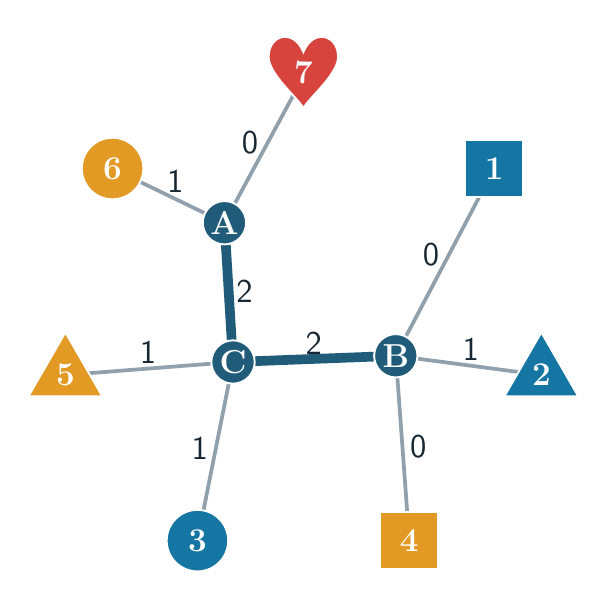
\begin{tikzpicture}[x=1cm,y=1cm]
\coordinate (orbit-1-v1) at (2.42368,1.93282);
\coordinate (orbit-1-v2) at (3.02228,-0.68981);
\coordinate (orbit-1-v3) at (-1.34504,-2.79300);
\coordinate (orbit-1-v4) at (1.34504,-2.79300);
\coordinate (orbit-1-v5) at (-3.02228,-0.68981);
\coordinate (orbit-1-v6) at (-2.42368,1.93282);
\coordinate (orbit-1-v7) at (0.00000,3.10000);
\coordinate (orbit-1-v8) at (-1.00210,1.24411);
\coordinate (orbit-1-v9) at (1.17388,-0.44566);
\coordinate (orbit-1-v10) at (-0.89343,-0.52447);
\draw[internal edge] (orbit-1-v8)--node[mini length,pos=0.5] {\(2\)}(orbit-1-v10);
\draw[internal edge] (orbit-1-v9)--node[mini length,pos=0.5] {\(2\)}(orbit-1-v10);
\draw[pendant edge] (orbit-1-v1)--node[mini length,pos=0.5] {\(0\)}(orbit-1-v9);
\draw[pendant edge] (orbit-1-v2)--node[mini length,pos=0.5] {\(1\)}(orbit-1-v9);
\draw[pendant edge] (orbit-1-v3)--node[mini length,pos=0.5] {\(1\)}(orbit-1-v10);
\draw[pendant edge] (orbit-1-v4)--node[mini length,pos=0.5] {\(0\)}(orbit-1-v9);
\draw[pendant edge] (orbit-1-v5)--node[mini length,pos=0.5] {\(1\)}(orbit-1-v10);
\draw[pendant edge] (orbit-1-v6)--node[mini length,pos=0.5] {\(1\)}(orbit-1-v8);
\draw[pendant edge] (orbit-1-v7)--node[mini length,pos=0.5] {\(0\)}(orbit-1-v8);
\node[orbit lettered vertex] at (orbit-1-v8) {A};
\node[orbit lettered vertex] at (orbit-1-v9) {B};
\node[orbit lettered vertex] at (orbit-1-v10) {C};
\taxonone{orbit-1-v1}
\taxontwo{orbit-1-v2}
\taxonthree{orbit-1-v3}
\taxonfour{orbit-1-v4}
\taxonfive{orbit-1-v5}
\taxonsix{orbit-1-v6}
\taxonseven{orbit-1-v7}
\end{tikzpicture}
\end{minipage}\par
\begin{minipage}[t][0.228\textheight][t]{\linewidth}
\centering\vspace{0pt}
\begin{tikzpicture}
\node[atlas box,inner xsep=1.8mm,inner ysep=1.2mm,text width=.94\linewidth,align=left] {%
\AtlasOrbitSplit{%
\vspace*{-2mm}\mbox{{\large\bfseries [O2]}\hspace{3mm}{\small\color{muted}size 6}}%
}{%
{\small{\color{muted}\underline{2}, 25, 26, 28, 31, 32}\rule[-3mm]{0pt}{3mm}}%
}%
};
\end{tikzpicture}\par\vspace{0mm}
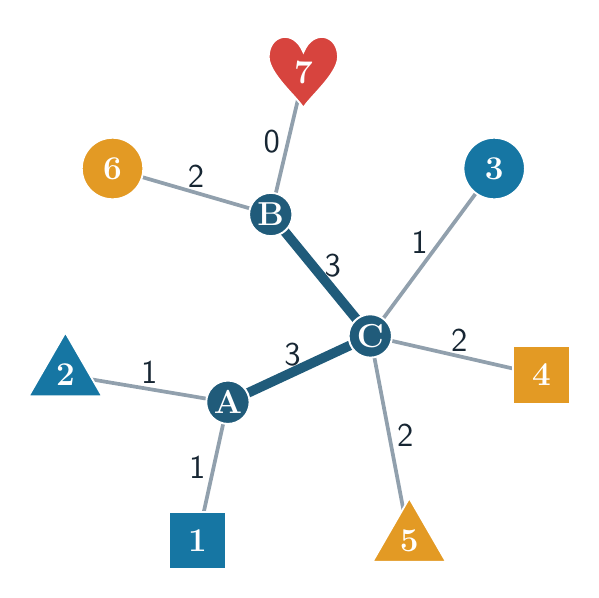
\begin{tikzpicture}[x=1cm,y=1cm]
\coordinate (orbit-2-v1) at (-1.34504,-2.79300);
\coordinate (orbit-2-v2) at (-3.02228,-0.68981);
\coordinate (orbit-2-v3) at (2.42368,1.93282);
\coordinate (orbit-2-v4) at (3.02228,-0.68981);
\coordinate (orbit-2-v5) at (1.34504,-2.79300);
\coordinate (orbit-2-v6) at (-2.42368,1.93282);
\coordinate (orbit-2-v7) at (0.00000,3.10000);
\coordinate (orbit-2-v8) at (-0.95817,-1.03560);
\coordinate (orbit-2-v9) at (-0.41396,1.34878);
\coordinate (orbit-2-v10) at (0.84974,-0.19395);
\draw[internal edge] (orbit-2-v8)--node[mini length,pos=0.5] {\(3\)}(orbit-2-v10);
\draw[internal edge] (orbit-2-v9)--node[mini length,pos=0.5] {\(3\)}(orbit-2-v10);
\draw[pendant edge] (orbit-2-v1)--node[mini length,pos=0.5] {\(1\)}(orbit-2-v8);
\draw[pendant edge] (orbit-2-v2)--node[mini length,pos=0.5] {\(1\)}(orbit-2-v8);
\draw[pendant edge] (orbit-2-v3)--node[mini length,pos=0.5] {\(1\)}(orbit-2-v10);
\draw[pendant edge] (orbit-2-v4)--node[mini length,pos=0.5] {\(2\)}(orbit-2-v10);
\draw[pendant edge] (orbit-2-v5)--node[mini length,pos=0.5] {\(2\)}(orbit-2-v10);
\draw[pendant edge] (orbit-2-v6)--node[mini length,pos=0.5] {\(2\)}(orbit-2-v9);
\draw[pendant edge] (orbit-2-v7)--node[mini length,pos=0.5] {\(0\)}(orbit-2-v9);
\node[orbit lettered vertex] at (orbit-2-v8) {A};
\node[orbit lettered vertex] at (orbit-2-v9) {B};
\node[orbit lettered vertex] at (orbit-2-v10) {C};
\taxonone{orbit-2-v1}
\taxontwo{orbit-2-v2}
\taxonthree{orbit-2-v3}
\taxonfour{orbit-2-v4}
\taxonfive{orbit-2-v5}
\taxonsix{orbit-2-v6}
\taxonseven{orbit-2-v7}
\end{tikzpicture}
\end{minipage}\par
\begin{minipage}[t][0.228\textheight][t]{\linewidth}
\centering\vspace{0pt}
\begin{tikzpicture}
\node[atlas box,inner xsep=1.8mm,inner ysep=1.2mm,text width=.94\linewidth,align=left] {%
\AtlasOrbitSplit{%
\vspace*{-2mm}\mbox{{\large\bfseries [O3]}\hspace{3mm}{\small\color{muted}size 6}}%
}{%
{\small{\color{muted}\underline{3}, 5, 16, 27, 46, 47}\rule[-3mm]{0pt}{3mm}}%
}%
};
\end{tikzpicture}\par\vspace{0mm}
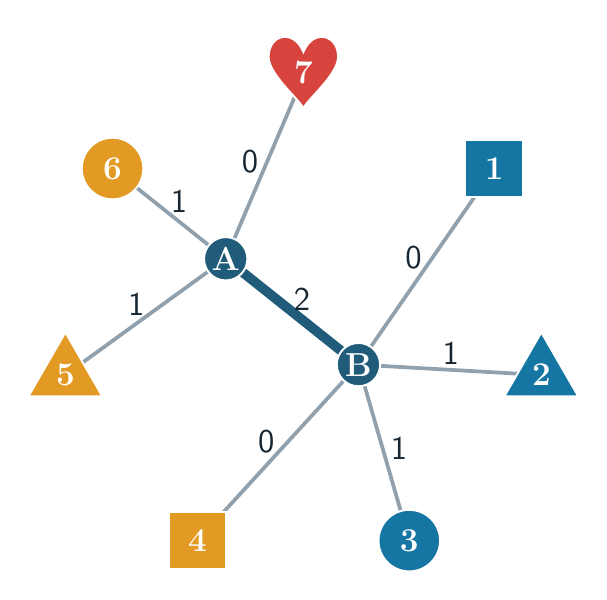
\begin{tikzpicture}[x=1cm,y=1cm]
\coordinate (orbit-3-v1) at (2.42368,1.93282);
\coordinate (orbit-3-v2) at (3.02228,-0.68981);
\coordinate (orbit-3-v3) at (1.34504,-2.79300);
\coordinate (orbit-3-v4) at (-1.34504,-2.79300);
\coordinate (orbit-3-v5) at (-3.02228,-0.68981);
\coordinate (orbit-3-v6) at (-2.42368,1.93282);
\coordinate (orbit-3-v7) at (0.00000,3.10000);
\coordinate (orbit-3-v8) at (-0.98600,0.78631);
\coordinate (orbit-3-v9) at (0.69938,-0.55773);
\draw[internal edge] (orbit-3-v8)--node[mini length,pos=0.5] {\(2\)}(orbit-3-v9);
\draw[pendant edge] (orbit-3-v1)--node[mini length,pos=0.5] {\(0\)}(orbit-3-v9);
\draw[pendant edge] (orbit-3-v2)--node[mini length,pos=0.5] {\(1\)}(orbit-3-v9);
\draw[pendant edge] (orbit-3-v3)--node[mini length,pos=0.5] {\(1\)}(orbit-3-v9);
\draw[pendant edge] (orbit-3-v4)--node[mini length,pos=0.5] {\(0\)}(orbit-3-v9);
\draw[pendant edge] (orbit-3-v5)--node[mini length,pos=0.5] {\(1\)}(orbit-3-v8);
\draw[pendant edge] (orbit-3-v6)--node[mini length,pos=0.5] {\(1\)}(orbit-3-v8);
\draw[pendant edge] (orbit-3-v7)--node[mini length,pos=0.5] {\(0\)}(orbit-3-v8);
\node[orbit lettered vertex] at (orbit-3-v8) {A};
\node[orbit lettered vertex] at (orbit-3-v9) {B};
\taxonone{orbit-3-v1}
\taxontwo{orbit-3-v2}
\taxonthree{orbit-3-v3}
\taxonfour{orbit-3-v4}
\taxonfive{orbit-3-v5}
\taxonsix{orbit-3-v6}
\taxonseven{orbit-3-v7}
\end{tikzpicture}
\end{minipage}\par
\begin{minipage}[t][0.228\textheight][t]{\linewidth}
\centering\vspace{0pt}
\begin{tikzpicture}
\node[atlas box,inner xsep=1.8mm,inner ysep=1.2mm,text width=.94\linewidth,align=left] {%
\AtlasOrbitSplit{%
\vspace*{-2mm}\mbox{{\large\bfseries [O4]}\hspace{3mm}{\small\color{muted}size 6}}%
}{%
{\small{\color{muted}\underline{6}, 7, 11, 12, 40, 41}\rule[-3mm]{0pt}{3mm}}%
}%
};
\end{tikzpicture}\par\vspace{0mm}
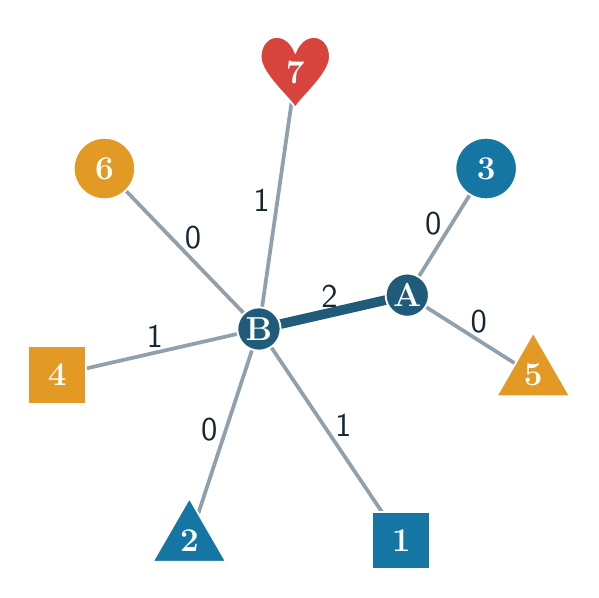
\begin{tikzpicture}[x=1cm,y=1cm]
\coordinate (orbit-4-v1) at (1.34504,-2.79300);
\coordinate (orbit-4-v2) at (-1.34504,-2.79300);
\coordinate (orbit-4-v3) at (2.42368,1.93282);
\coordinate (orbit-4-v4) at (-3.02228,-0.68981);
\coordinate (orbit-4-v5) at (3.02228,-0.68981);
\coordinate (orbit-4-v6) at (-2.42368,1.93282);
\coordinate (orbit-4-v7) at (0.00000,3.10000);
\coordinate (orbit-4-v8) at (1.42236,0.32464);
\coordinate (orbit-4-v9) at (-0.46130,-0.10529);
\draw[internal edge] (orbit-4-v8)--node[mini length,pos=0.5] {\(2\)}(orbit-4-v9);
\draw[pendant edge] (orbit-4-v1)--node[mini length,pos=0.5] {\(1\)}(orbit-4-v9);
\draw[pendant edge] (orbit-4-v2)--node[mini length,pos=0.5] {\(0\)}(orbit-4-v9);
\draw[pendant edge] (orbit-4-v3)--node[mini length,pos=0.5] {\(0\)}(orbit-4-v8);
\draw[pendant edge] (orbit-4-v4)--node[mini length,pos=0.5] {\(1\)}(orbit-4-v9);
\draw[pendant edge] (orbit-4-v5)--node[mini length,pos=0.5] {\(0\)}(orbit-4-v8);
\draw[pendant edge] (orbit-4-v6)--node[mini length,pos=0.5] {\(0\)}(orbit-4-v9);
\draw[pendant edge] (orbit-4-v7)--node[mini length,pos=0.5] {\(1\)}(orbit-4-v9);
\node[orbit lettered vertex] at (orbit-4-v8) {A};
\node[orbit lettered vertex] at (orbit-4-v9) {B};
\taxonone{orbit-4-v1}
\taxontwo{orbit-4-v2}
\taxonthree{orbit-4-v3}
\taxonfour{orbit-4-v4}
\taxonfive{orbit-4-v5}
\taxonsix{orbit-4-v6}
\taxonseven{orbit-4-v7}
\end{tikzpicture}
\end{minipage}\par
\end{minipage}
\hfill
\begin{minipage}[t]{0.318\textwidth}\vspace{0pt}
\begin{minipage}[t][0.228\textheight][t]{\linewidth}
\centering\vspace{0pt}
\begin{tikzpicture}
\node[atlas box,inner xsep=1.8mm,inner ysep=1.2mm,text width=.94\linewidth,align=left] {%
\AtlasOrbitSplit{%
\vspace*{-2mm}\mbox{{\large\bfseries [O5]}\hspace{3mm}{\small\color{muted}size 3}}%
}{%
{\small{\color{muted}\underline{8}, 33, 34}\rule[-3mm]{0pt}{3mm}}%
}%
};
\end{tikzpicture}\par\vspace{0mm}
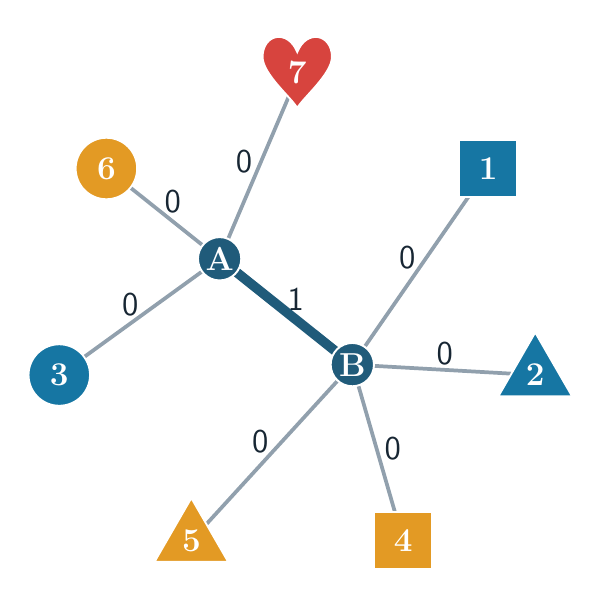
\begin{tikzpicture}[x=1cm,y=1cm]
\coordinate (orbit-5-v1) at (2.42368,1.93282);
\coordinate (orbit-5-v2) at (3.02228,-0.68981);
\coordinate (orbit-5-v3) at (-3.02228,-0.68981);
\coordinate (orbit-5-v4) at (1.34504,-2.79300);
\coordinate (orbit-5-v5) at (-1.34504,-2.79300);
\coordinate (orbit-5-v6) at (-2.42368,1.93282);
\coordinate (orbit-5-v7) at (0.00000,3.10000);
\coordinate (orbit-5-v8) at (-0.98600,0.78631);
\coordinate (orbit-5-v9) at (0.69938,-0.55773);
\draw[internal edge] (orbit-5-v8)--node[mini length,pos=0.5] {\(1\)}(orbit-5-v9);
\draw[pendant edge] (orbit-5-v1)--node[mini length,pos=0.5] {\(0\)}(orbit-5-v9);
\draw[pendant edge] (orbit-5-v2)--node[mini length,pos=0.5] {\(0\)}(orbit-5-v9);
\draw[pendant edge] (orbit-5-v3)--node[mini length,pos=0.5] {\(0\)}(orbit-5-v8);
\draw[pendant edge] (orbit-5-v4)--node[mini length,pos=0.5] {\(0\)}(orbit-5-v9);
\draw[pendant edge] (orbit-5-v5)--node[mini length,pos=0.5] {\(0\)}(orbit-5-v9);
\draw[pendant edge] (orbit-5-v6)--node[mini length,pos=0.5] {\(0\)}(orbit-5-v8);
\draw[pendant edge] (orbit-5-v7)--node[mini length,pos=0.5] {\(0\)}(orbit-5-v8);
\node[orbit lettered vertex] at (orbit-5-v8) {A};
\node[orbit lettered vertex] at (orbit-5-v9) {B};
\taxonone{orbit-5-v1}
\taxontwo{orbit-5-v2}
\taxonthree{orbit-5-v3}
\taxonfour{orbit-5-v4}
\taxonfive{orbit-5-v5}
\taxonsix{orbit-5-v6}
\taxonseven{orbit-5-v7}
\end{tikzpicture}
\end{minipage}\par
\begin{minipage}[t][0.228\textheight][t]{\linewidth}
\centering\vspace{0pt}
\begin{tikzpicture}
\node[atlas box,inner xsep=1.8mm,inner ysep=1.2mm,text width=.94\linewidth,align=left] {%
\AtlasOrbitSplit{%
\vspace*{-2mm}\mbox{{\large\bfseries [O6]}\hspace{3mm}{\small\color{muted}size 3}}%
}{%
{\small{\color{muted}\underline{9}, 10, 30}\rule[-3mm]{0pt}{3mm}}%
}%
};
\end{tikzpicture}\par\vspace{0mm}
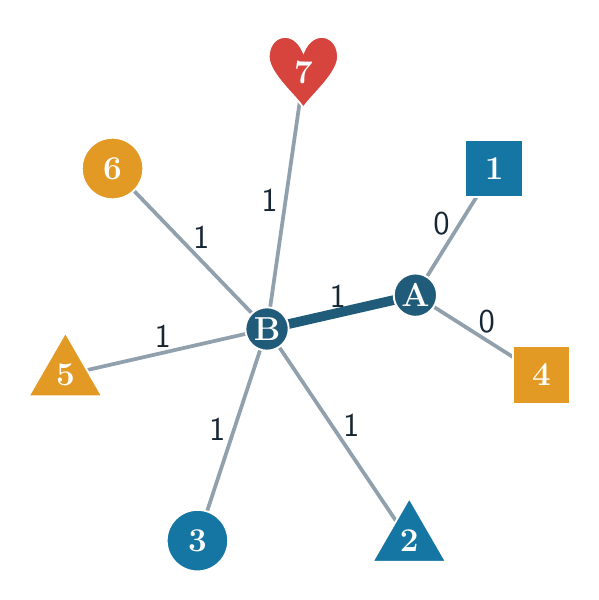
\begin{tikzpicture}[x=1cm,y=1cm]
\coordinate (orbit-6-v1) at (2.42368,1.93282);
\coordinate (orbit-6-v2) at (1.34504,-2.79300);
\coordinate (orbit-6-v3) at (-1.34504,-2.79300);
\coordinate (orbit-6-v4) at (3.02228,-0.68981);
\coordinate (orbit-6-v5) at (-3.02228,-0.68981);
\coordinate (orbit-6-v6) at (-2.42368,1.93282);
\coordinate (orbit-6-v7) at (0.00000,3.10000);
\coordinate (orbit-6-v8) at (1.42236,0.32464);
\coordinate (orbit-6-v9) at (-0.46130,-0.10529);
\draw[internal edge] (orbit-6-v8)--node[mini length,pos=0.5] {\(1\)}(orbit-6-v9);
\draw[pendant edge] (orbit-6-v1)--node[mini length,pos=0.5] {\(0\)}(orbit-6-v8);
\draw[pendant edge] (orbit-6-v2)--node[mini length,pos=0.5] {\(1\)}(orbit-6-v9);
\draw[pendant edge] (orbit-6-v3)--node[mini length,pos=0.5] {\(1\)}(orbit-6-v9);
\draw[pendant edge] (orbit-6-v4)--node[mini length,pos=0.5] {\(0\)}(orbit-6-v8);
\draw[pendant edge] (orbit-6-v5)--node[mini length,pos=0.5] {\(1\)}(orbit-6-v9);
\draw[pendant edge] (orbit-6-v6)--node[mini length,pos=0.5] {\(1\)}(orbit-6-v9);
\draw[pendant edge] (orbit-6-v7)--node[mini length,pos=0.5] {\(1\)}(orbit-6-v9);
\node[orbit lettered vertex] at (orbit-6-v8) {A};
\node[orbit lettered vertex] at (orbit-6-v9) {B};
\taxonone{orbit-6-v1}
\taxontwo{orbit-6-v2}
\taxonthree{orbit-6-v3}
\taxonfour{orbit-6-v4}
\taxonfive{orbit-6-v5}
\taxonsix{orbit-6-v6}
\taxonseven{orbit-6-v7}
\end{tikzpicture}
\end{minipage}\par
\begin{minipage}[t][0.228\textheight][t]{\linewidth}
\centering\vspace{0pt}
\begin{tikzpicture}
\node[atlas box,inner xsep=1.8mm,inner ysep=1.2mm,text width=.94\linewidth,align=left] {%
\AtlasOrbitSplit{%
\vspace*{-2mm}\mbox{{\large\bfseries [O7]}\hspace{3mm}{\small\color{muted}size 6}}%
}{%
{\small{\color{muted}\underline{13}, 17, 19, 20, 44, 45}\rule[-3mm]{0pt}{3mm}}%
}%
};
\end{tikzpicture}\par\vspace{0mm}
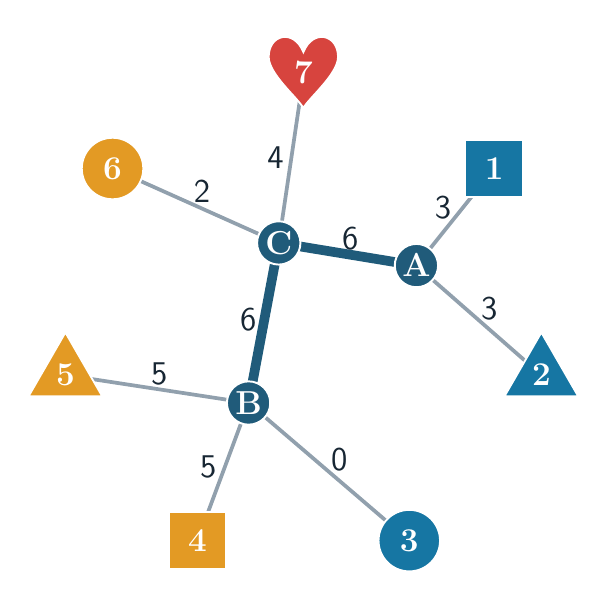
\begin{tikzpicture}[x=1cm,y=1cm]
\coordinate (orbit-7-v1) at (2.42368,1.93282);
\coordinate (orbit-7-v2) at (3.02228,-0.68981);
\coordinate (orbit-7-v3) at (1.34504,-2.79300);
\coordinate (orbit-7-v4) at (-1.34504,-2.79300);
\coordinate (orbit-7-v5) at (-3.02228,-0.68981);
\coordinate (orbit-7-v6) at (-2.42368,1.93282);
\coordinate (orbit-7-v7) at (0.00000,3.10000);
\coordinate (orbit-7-v8) at (1.43590,0.70014);
\coordinate (orbit-7-v9) at (-0.69570,-1.04528);
\coordinate (orbit-7-v10) at (-0.31252,0.98774);
\draw[internal edge] (orbit-7-v8)--node[mini length,pos=0.5] {\(6\)}(orbit-7-v10);
\draw[internal edge] (orbit-7-v9)--node[mini length,pos=0.5] {\(6\)}(orbit-7-v10);
\draw[pendant edge] (orbit-7-v1)--node[mini length,pos=0.5] {\(3\)}(orbit-7-v8);
\draw[pendant edge] (orbit-7-v2)--node[mini length,pos=0.5] {\(3\)}(orbit-7-v8);
\draw[pendant edge] (orbit-7-v3)--node[mini length,pos=0.5] {\(0\)}(orbit-7-v9);
\draw[pendant edge] (orbit-7-v4)--node[mini length,pos=0.5] {\(5\)}(orbit-7-v9);
\draw[pendant edge] (orbit-7-v5)--node[mini length,pos=0.5] {\(5\)}(orbit-7-v9);
\draw[pendant edge] (orbit-7-v6)--node[mini length,pos=0.5] {\(2\)}(orbit-7-v10);
\draw[pendant edge] (orbit-7-v7)--node[mini length,pos=0.5] {\(4\)}(orbit-7-v10);
\node[orbit lettered vertex] at (orbit-7-v8) {A};
\node[orbit lettered vertex] at (orbit-7-v9) {B};
\node[orbit lettered vertex] at (orbit-7-v10) {C};
\taxonone{orbit-7-v1}
\taxontwo{orbit-7-v2}
\taxonthree{orbit-7-v3}
\taxonfour{orbit-7-v4}
\taxonfive{orbit-7-v5}
\taxonsix{orbit-7-v6}
\taxonseven{orbit-7-v7}
\end{tikzpicture}
\end{minipage}\par
\begin{minipage}[t][0.228\textheight][t]{\linewidth}
\centering\vspace{0pt}
\begin{tikzpicture}
\node[atlas box,inner xsep=1.8mm,inner ysep=1.2mm,text width=.94\linewidth,align=left] {%
\AtlasOrbitSplit{%
\vspace*{-2mm}\mbox{{\large\bfseries [O8]}\hspace{3mm}{\small\color{muted}size 3}}%
}{%
{\small{\color{muted}\underline{14}, 21, 22}\rule[-3mm]{0pt}{3mm}}%
}%
};
\end{tikzpicture}\par\vspace{0mm}
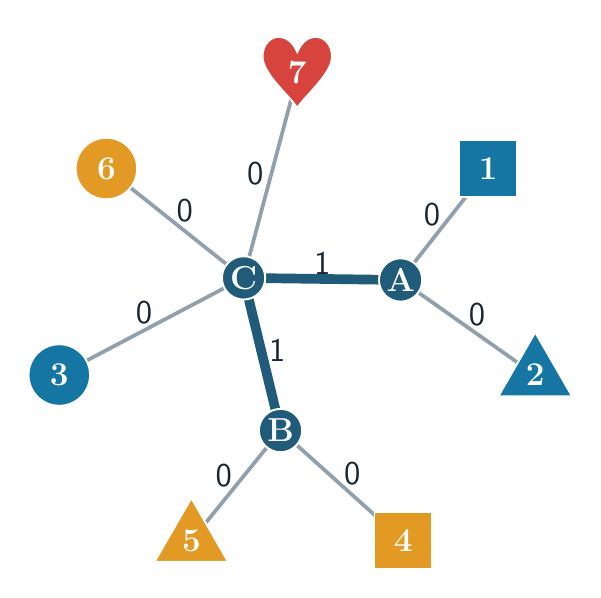
\begin{tikzpicture}[x=1cm,y=1cm]
\coordinate (orbit-8-v1) at (2.42368,1.93282);
\coordinate (orbit-8-v2) at (3.02228,-0.68981);
\coordinate (orbit-8-v3) at (-3.02228,-0.68981);
\coordinate (orbit-8-v4) at (1.34504,-2.79300);
\coordinate (orbit-8-v5) at (-1.34504,-2.79300);
\coordinate (orbit-8-v6) at (-2.42368,1.93282);
\coordinate (orbit-8-v7) at (0.00000,3.10000);
\coordinate (orbit-8-v8) at (1.31261,0.51731);
\coordinate (orbit-8-v9) at (-0.21225,-1.39482);
\coordinate (orbit-8-v10) at (-0.68144,0.54343);
\draw[internal edge] (orbit-8-v8)--node[mini length,pos=0.5] {\(1\)}(orbit-8-v10);
\draw[internal edge] (orbit-8-v9)--node[mini length,pos=0.5] {\(1\)}(orbit-8-v10);
\draw[pendant edge] (orbit-8-v1)--node[mini length,pos=0.5] {\(0\)}(orbit-8-v8);
\draw[pendant edge] (orbit-8-v2)--node[mini length,pos=0.5] {\(0\)}(orbit-8-v8);
\draw[pendant edge] (orbit-8-v3)--node[mini length,pos=0.5] {\(0\)}(orbit-8-v10);
\draw[pendant edge] (orbit-8-v4)--node[mini length,pos=0.5] {\(0\)}(orbit-8-v9);
\draw[pendant edge] (orbit-8-v5)--node[mini length,pos=0.5] {\(0\)}(orbit-8-v9);
\draw[pendant edge] (orbit-8-v6)--node[mini length,pos=0.5] {\(0\)}(orbit-8-v10);
\draw[pendant edge] (orbit-8-v7)--node[mini length,pos=0.5] {\(0\)}(orbit-8-v10);
\node[orbit lettered vertex] at (orbit-8-v8) {A};
\node[orbit lettered vertex] at (orbit-8-v9) {B};
\node[orbit lettered vertex] at (orbit-8-v10) {C};
\taxonone{orbit-8-v1}
\taxontwo{orbit-8-v2}
\taxonthree{orbit-8-v3}
\taxonfour{orbit-8-v4}
\taxonfive{orbit-8-v5}
\taxonsix{orbit-8-v6}
\taxonseven{orbit-8-v7}
\end{tikzpicture}
\end{minipage}\par
\end{minipage}
\hfill
\begin{minipage}[t]{0.318\textwidth}\vspace{0pt}
\begin{minipage}[t][0.228\textheight][t]{\linewidth}
\centering\vspace{0pt}
\begin{tikzpicture}
\node[atlas box,inner xsep=1.8mm,inner ysep=1.2mm,text width=.94\linewidth,align=left] {%
\AtlasOrbitSplit{%
\vspace*{-2mm}\mbox{{\large\bfseries [O9]}\hspace{3mm}{\small\color{muted}size 2}}%
}{%
{\small{\color{muted}\underline{15}, 29}\rule[-3mm]{0pt}{3mm}}%
}%
};
\end{tikzpicture}\par\vspace{0mm}
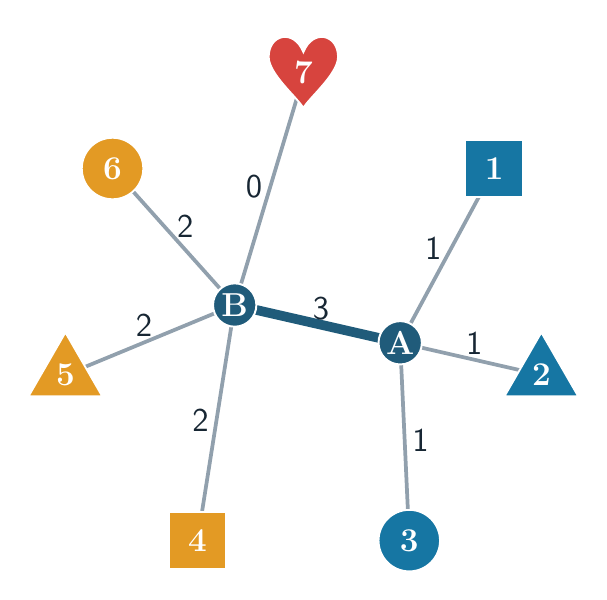
\begin{tikzpicture}[x=1cm,y=1cm]
\coordinate (orbit-9-v1) at (2.42368,1.93282);
\coordinate (orbit-9-v2) at (3.02228,-0.68981);
\coordinate (orbit-9-v3) at (1.34504,-2.79300);
\coordinate (orbit-9-v4) at (-1.34504,-2.79300);
\coordinate (orbit-9-v5) at (-3.02228,-0.68981);
\coordinate (orbit-9-v6) at (-2.42368,1.93282);
\coordinate (orbit-9-v7) at (0.00000,3.10000);
\coordinate (orbit-9-v8) at (1.22953,-0.28063);
\coordinate (orbit-9-v9) at (-0.87211,0.19905);
\draw[internal edge] (orbit-9-v8)--node[mini length,pos=0.5] {\(3\)}(orbit-9-v9);
\draw[pendant edge] (orbit-9-v1)--node[mini length,pos=0.5] {\(1\)}(orbit-9-v8);
\draw[pendant edge] (orbit-9-v2)--node[mini length,pos=0.5] {\(1\)}(orbit-9-v8);
\draw[pendant edge] (orbit-9-v3)--node[mini length,pos=0.5] {\(1\)}(orbit-9-v8);
\draw[pendant edge] (orbit-9-v4)--node[mini length,pos=0.5] {\(2\)}(orbit-9-v9);
\draw[pendant edge] (orbit-9-v5)--node[mini length,pos=0.5] {\(2\)}(orbit-9-v9);
\draw[pendant edge] (orbit-9-v6)--node[mini length,pos=0.5] {\(2\)}(orbit-9-v9);
\draw[pendant edge] (orbit-9-v7)--node[mini length,pos=0.5] {\(0\)}(orbit-9-v9);
\node[orbit lettered vertex] at (orbit-9-v8) {A};
\node[orbit lettered vertex] at (orbit-9-v9) {B};
\taxonone{orbit-9-v1}
\taxontwo{orbit-9-v2}
\taxonthree{orbit-9-v3}
\taxonfour{orbit-9-v4}
\taxonfive{orbit-9-v5}
\taxonsix{orbit-9-v6}
\taxonseven{orbit-9-v7}
\end{tikzpicture}
\end{minipage}\par
\begin{minipage}[t][0.228\textheight][t]{\linewidth}
\centering\vspace{0pt}
\begin{tikzpicture}
\node[atlas box,inner xsep=1.8mm,inner ysep=1.2mm,text width=.94\linewidth,align=left] {%
\AtlasOrbitSplit{%
\vspace*{-2mm}\mbox{{\large\bfseries [O10]}\hspace{3mm}{\small\color{muted}size 3}}%
}{%
{\small{\color{muted}\underline{18}, 35, 36}\rule[-3mm]{0pt}{3mm}}%
}%
};
\end{tikzpicture}\par\vspace{0mm}
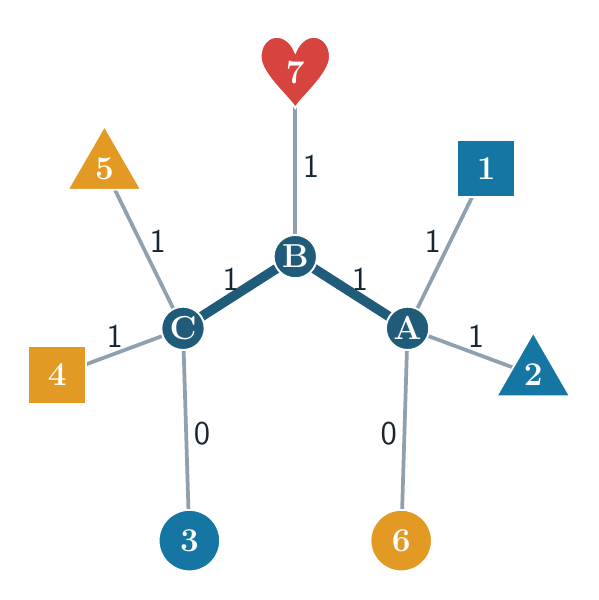
\begin{tikzpicture}[x=1cm,y=1cm]
\coordinate (orbit-10-v1) at (2.42368,1.93282);
\coordinate (orbit-10-v2) at (3.02228,-0.68981);
\coordinate (orbit-10-v3) at (-1.34504,-2.79300);
\coordinate (orbit-10-v4) at (-3.02228,-0.68981);
\coordinate (orbit-10-v5) at (-2.42368,1.93282);
\coordinate (orbit-10-v6) at (1.34504,-2.79300);
\coordinate (orbit-10-v7) at (0.00000,3.10000);
\coordinate (orbit-10-v8) at (1.42611,-0.09713);
\coordinate (orbit-10-v9) at (0.00000,0.81427);
\coordinate (orbit-10-v10) at (-1.42611,-0.09713);
\draw[internal edge] (orbit-10-v8)--node[mini length,pos=0.5] {\(1\)}(orbit-10-v9);
\draw[internal edge] (orbit-10-v9)--node[mini length,pos=0.5] {\(1\)}(orbit-10-v10);
\draw[pendant edge] (orbit-10-v1)--node[mini length,pos=0.5] {\(1\)}(orbit-10-v8);
\draw[pendant edge] (orbit-10-v2)--node[mini length,pos=0.5] {\(1\)}(orbit-10-v8);
\draw[pendant edge] (orbit-10-v3)--node[mini length,pos=0.5] {\(0\)}(orbit-10-v10);
\draw[pendant edge] (orbit-10-v4)--node[mini length,pos=0.5] {\(1\)}(orbit-10-v10);
\draw[pendant edge] (orbit-10-v5)--node[mini length,pos=0.5] {\(1\)}(orbit-10-v10);
\draw[pendant edge] (orbit-10-v6)--node[mini length,pos=0.5] {\(0\)}(orbit-10-v8);
\draw[pendant edge] (orbit-10-v7)--node[mini length,pos=0.5] {\(1\)}(orbit-10-v9);
\node[orbit lettered vertex] at (orbit-10-v8) {A};
\node[orbit lettered vertex] at (orbit-10-v9) {B};
\node[orbit lettered vertex] at (orbit-10-v10) {C};
\taxonone{orbit-10-v1}
\taxontwo{orbit-10-v2}
\taxonthree{orbit-10-v3}
\taxonfour{orbit-10-v4}
\taxonfive{orbit-10-v5}
\taxonsix{orbit-10-v6}
\taxonseven{orbit-10-v7}
\end{tikzpicture}
\end{minipage}\par
\begin{minipage}[t][0.228\textheight][t]{\linewidth}
\centering\vspace{0pt}
\begin{tikzpicture}
\node[atlas box,inner xsep=1.8mm,inner ysep=1.2mm,text width=.94\linewidth,align=left] {%
\AtlasOrbitSplit{%
\vspace*{-2mm}\mbox{{\large\bfseries [O11]}\hspace{3mm}{\small\color{muted}size 1}}%
}{%
{\small{\color{muted}\underline{37}}\rule[-3mm]{0pt}{3mm}}%
}%
};
\end{tikzpicture}\par\vspace{0mm}
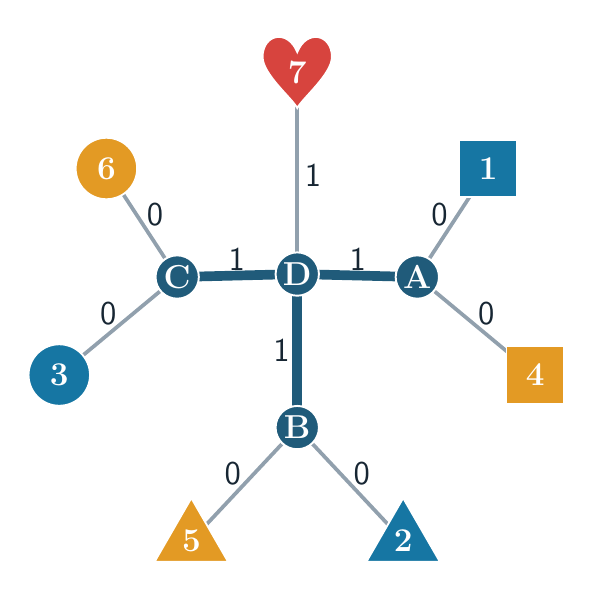
\begin{tikzpicture}[x=1cm,y=1cm]
\coordinate (orbit-11-v1) at (2.42368,1.93282);
\coordinate (orbit-11-v2) at (1.34504,-2.79300);
\coordinate (orbit-11-v3) at (-3.02228,-0.68981);
\coordinate (orbit-11-v4) at (3.02228,-0.68981);
\coordinate (orbit-11-v5) at (-1.34504,-2.79300);
\coordinate (orbit-11-v6) at (-2.42368,1.93282);
\coordinate (orbit-11-v7) at (0.00000,3.10000);
\coordinate (orbit-11-v8) at (1.52487,0.55471);
\coordinate (orbit-11-v9) at (0.00000,-1.35742);
\coordinate (orbit-11-v10) at (-1.52487,0.55471);
\coordinate (orbit-11-v11) at (0.00000,0.59244);
\draw[internal edge] (orbit-11-v8)--node[mini length,pos=0.5] {\(1\)}(orbit-11-v11);
\draw[internal edge] (orbit-11-v9)--node[mini length,pos=0.5] {\(1\)}(orbit-11-v11);
\draw[internal edge] (orbit-11-v10)--node[mini length,pos=0.5] {\(1\)}(orbit-11-v11);
\draw[pendant edge] (orbit-11-v1)--node[mini length,pos=0.5] {\(0\)}(orbit-11-v8);
\draw[pendant edge] (orbit-11-v2)--node[mini length,pos=0.5] {\(0\)}(orbit-11-v9);
\draw[pendant edge] (orbit-11-v3)--node[mini length,pos=0.5] {\(0\)}(orbit-11-v10);
\draw[pendant edge] (orbit-11-v4)--node[mini length,pos=0.5] {\(0\)}(orbit-11-v8);
\draw[pendant edge] (orbit-11-v5)--node[mini length,pos=0.5] {\(0\)}(orbit-11-v9);
\draw[pendant edge] (orbit-11-v6)--node[mini length,pos=0.5] {\(0\)}(orbit-11-v10);
\draw[pendant edge] (orbit-11-v7)--node[mini length,pos=0.5] {\(1\)}(orbit-11-v11);
\node[orbit lettered vertex] at (orbit-11-v8) {A};
\node[orbit lettered vertex] at (orbit-11-v9) {B};
\node[orbit lettered vertex] at (orbit-11-v10) {C};
\node[orbit lettered vertex] at (orbit-11-v11) {D};
\taxonone{orbit-11-v1}
\taxontwo{orbit-11-v2}
\taxonthree{orbit-11-v3}
\taxonfour{orbit-11-v4}
\taxonfive{orbit-11-v5}
\taxonsix{orbit-11-v6}
\taxonseven{orbit-11-v7}
\end{tikzpicture}
\end{minipage}\par
\begin{minipage}[t][0.228\textheight][t]{\linewidth}
\centering\vspace{0pt}
\begin{tikzpicture}
\node[atlas box,inner xsep=1.8mm,inner ysep=1.2mm,text width=.94\linewidth,align=left] {%
\AtlasOrbitSplit{%
\vspace*{-2mm}\mbox{{\large\bfseries [O12]}\hspace{3mm}{\small\color{muted}size 3}}%
}{%
{\small{\color{animalblue}\bfseries\(\mathbb{F}_2\) only}\quad{\color{muted}\underline{52}, 53, 54}\rule[-3mm]{0pt}{3mm}}%
}%
};
\end{tikzpicture}\par\vspace{0mm}
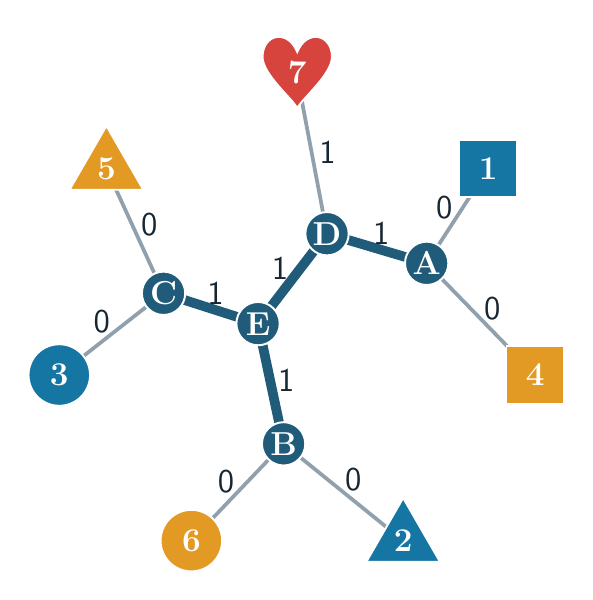
\begin{tikzpicture}[x=1cm,y=1cm]
\coordinate (orbit-12-v1) at (2.42368,1.93282);
\coordinate (orbit-12-v2) at (1.34504,-2.79300);
\coordinate (orbit-12-v3) at (-3.02228,-0.68981);
\coordinate (orbit-12-v4) at (3.02228,-0.68981);
\coordinate (orbit-12-v5) at (-2.42368,1.93282);
\coordinate (orbit-12-v6) at (-1.34504,-2.79300);
\coordinate (orbit-12-v7) at (0.00000,3.10000);
\coordinate (orbit-12-v8) at (1.64352,0.72865);
\coordinate (orbit-12-v9) at (-0.17334,-1.56407);
\coordinate (orbit-12-v10) at (-1.69821,0.34805);
\coordinate (orbit-12-v11) at (0.37820,1.10471);
\coordinate (orbit-12-v12) at (-0.49778,-0.03711);
\draw[internal edge] (orbit-12-v8)--node[mini length,pos=0.5] {\(1\)}(orbit-12-v11);
\draw[internal edge] (orbit-12-v9)--node[mini length,pos=0.5] {\(1\)}(orbit-12-v12);
\draw[internal edge] (orbit-12-v10)--node[mini length,pos=0.5] {\(1\)}(orbit-12-v12);
\draw[internal edge] (orbit-12-v11)--node[mini length,pos=0.5] {\(1\)}(orbit-12-v12);
\draw[pendant edge] (orbit-12-v1)--node[mini length,pos=0.5] {\(0\)}(orbit-12-v8);
\draw[pendant edge] (orbit-12-v2)--node[mini length,pos=0.5] {\(0\)}(orbit-12-v9);
\draw[pendant edge] (orbit-12-v3)--node[mini length,pos=0.5] {\(0\)}(orbit-12-v10);
\draw[pendant edge] (orbit-12-v4)--node[mini length,pos=0.5] {\(0\)}(orbit-12-v8);
\draw[pendant edge] (orbit-12-v5)--node[mini length,pos=0.5] {\(0\)}(orbit-12-v10);
\draw[pendant edge] (orbit-12-v6)--node[mini length,pos=0.5] {\(0\)}(orbit-12-v9);
\draw[pendant edge] (orbit-12-v7)--node[mini length,pos=0.5] {\(1\)}(orbit-12-v11);
\node[orbit lettered vertex] at (orbit-12-v8) {A};
\node[orbit lettered vertex] at (orbit-12-v9) {B};
\node[orbit lettered vertex] at (orbit-12-v10) {C};
\node[orbit lettered vertex] at (orbit-12-v11) {D};
\node[orbit lettered vertex] at (orbit-12-v12) {E};
\taxonone{orbit-12-v1}
\taxontwo{orbit-12-v2}
\taxonthree{orbit-12-v3}
\taxonfour{orbit-12-v4}
\taxonfive{orbit-12-v5}
\taxonsix{orbit-12-v6}
\taxonseven{orbit-12-v7}
\end{tikzpicture}
\end{minipage}\par
\end{minipage}
\clearpage
\vspace*{-7mm}
{\LARGE\bfseries Smallest pieces}\hfill{\small\color{muted}drawn by polymake}\par\vspace{3mm}
\begin{minipage}[t]{.485\textwidth}\begin{atlaspanel}
{\LARGE\bfseries \(\mathrm{M}(3,5)\)}\hspace{3mm}{\large\color{muted}multiplex}\hfill{\large\(f=(6,10,6)\)}\par\vspace{3mm}
\begin{minipage}[c][13.0cm][c]{\linewidth}\centering
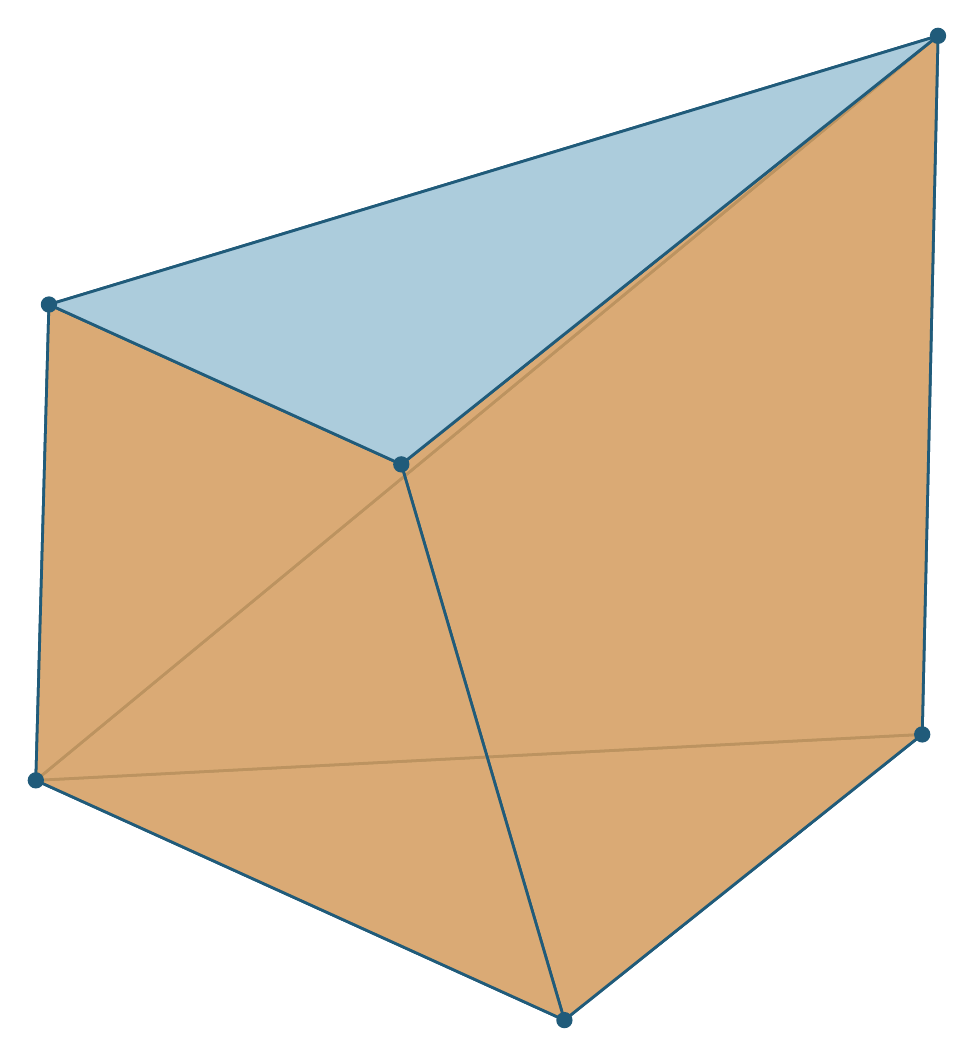
\begin{tikzpicture}[x  = {(0.9cm,-0.076cm)},
                    y  = {(-0.06cm,0.95cm)},
                    z  = {(-0.44cm,-0.29cm)},
                    scale = 2.3053,
                    color = {lightgray}]


  % DEF COORDINATES
  \coordinate (v0_piece1) at (-1.84615, 1.5503, 1.47929);
  \coordinate (v1_piece1) at (0.769231, 1.13609, 2.47337);
  \coordinate (v2_piece1) at (2.38462, 2.64497, -1.14793);
  \coordinate (v3_piece1) at (-3.15385, -1.93491, -0.556213);
  \coordinate (v4_piece1) at (0.769231, -2.55621, 0.934911);
  \coordinate (v5_piece1) at (1.84615, -1.5503, -1.47929);


  % VERTEXCOLOR
  \definecolor{vertexcolor_piece1}{rgb}{ 0.1255 0.3569 0.4784 }

  % DEF VERTEXSTYLES
  \tikzstyle{vertexstyle_piece1} = [circle, scale=0.625pt, fill=vertexcolor_piece1,]

  % FACETCOLOR
  \definecolor{facetcolor_piece1_0}{rgb}{ 0.6627 0.7922 0.8588 }
  \definecolor{facetcolor_piece1_1}{rgb}{ 0.8902 0.6314 0.3529 }

  % EDGECOLOR
  \definecolor{edgecolor_piece1}{rgb}{ 0.1255 0.3569 0.4784 }
  \tikzstyle{facetstyle_piece1_0} = [fill=facetcolor_piece1_1, fill opacity=0.8, draw=edgecolor_piece1, line width=1 pt, line cap=round, line join=round]
  \tikzstyle{facetstyle_piece1_1} = [fill=facetcolor_piece1_1, fill opacity=0.8, draw=edgecolor_piece1, line width=1 pt, line cap=round, line join=round]
  \tikzstyle{facetstyle_piece1_2} = [fill=facetcolor_piece1_0, fill opacity=0.8, draw=edgecolor_piece1, line width=1 pt, line cap=round, line join=round]
  \tikzstyle{facetstyle_piece1_3} = [fill=facetcolor_piece1_0, fill opacity=0.8, draw=edgecolor_piece1, line width=1 pt, line cap=round, line join=round]
  \tikzstyle{facetstyle_piece1_4} = [fill=facetcolor_piece1_0, fill opacity=0.8, draw=edgecolor_piece1, line width=1 pt, line cap=round, line join=round]
  \tikzstyle{facetstyle_piece1_5} = [fill=facetcolor_piece1_0, fill opacity=0.8, draw=edgecolor_piece1, line width=1 pt, line cap=round, line join=round]

  % FACES and EDGES and POINTS in the right order
  \draw[facetstyle_piece1_2] (v5_piece1) -- (v4_piece1) -- (v3_piece1) -- (v5_piece1) -- cycle;
  \draw[facetstyle_piece1_3] (v2_piece1) -- (v5_piece1) -- (v3_piece1) -- (v2_piece1) -- cycle;
  \draw[facetstyle_piece1_4] (v2_piece1) -- (v3_piece1) -- (v0_piece1) -- (v2_piece1) -- cycle;
  \draw[facetstyle_piece1_0] (v1_piece1) -- (v4_piece1) -- (v5_piece1) -- (v2_piece1) -- (v1_piece1) -- cycle;
  \draw[facetstyle_piece1_1] (v3_piece1) -- (v4_piece1) -- (v1_piece1) -- (v0_piece1) -- (v3_piece1) -- cycle;
  \draw[facetstyle_piece1_5] (v1_piece1) -- (v2_piece1) -- (v0_piece1) -- (v1_piece1) -- cycle;

  % POINTS
  \foreach \i in {0,3,1,4,5,2} {
    \node at (v\i_piece1) [vertexstyle_piece1] {};
  }


\end{tikzpicture}
\end{minipage}\par\vspace{3mm}
{\color{muted}In \(P_{8}\), \(P_{9}\), \(P_{10}\), \(P_{11}\), \(P_{12}\).}
\end{atlaspanel}\end{minipage}
\hfill
\begin{minipage}[t]{.485\textwidth}\begin{atlaspanel}
{\LARGE\bfseries \(\mathrm{AP}_{4}\)}\hspace{3mm}{\large\color{muted}square antiprism}\hfill{\large\(f=(8,16,10)\)}\par\vspace{3mm}
\begin{minipage}[c][13.0cm][c]{\linewidth}\centering
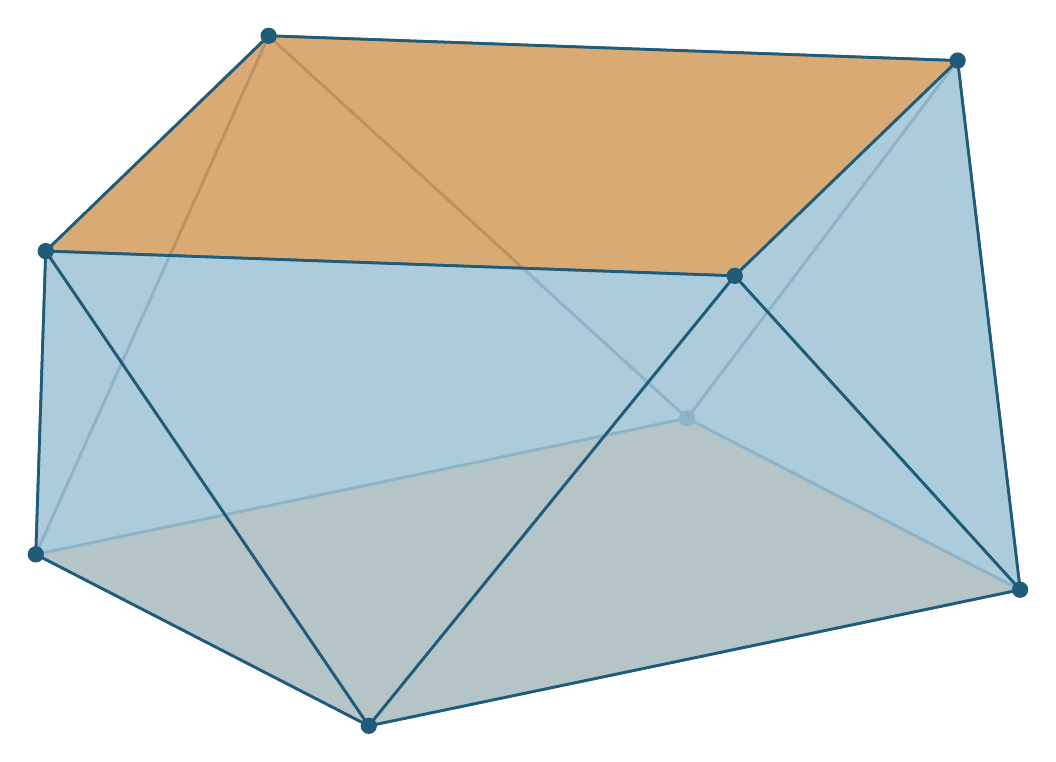
\begin{tikzpicture}[x  = {(0.9cm,-0.076cm)},
                    y  = {(-0.06cm,0.95cm)},
                    z  = {(-0.44cm,-0.29cm)},
                    scale = 2.3182,
                    color = {lightgray}]


  % DEF COORDINATES
  \coordinate (v0_piece2) at (0.4, 0, 2.8);
  \coordinate (v1_piece2) at (-2.8, 0, 0.4);
  \coordinate (v2_piece2) at (-0.4, 0, -2.8);
  \coordinate (v3_piece2) at (2.8, 0, -0.4);
  \coordinate (v4_piece2) at (2.24, 2.4, 1.68);
  \coordinate (v5_piece2) at (-1.68, 2.4, 2.24);
  \coordinate (v6_piece2) at (-2.24, 2.4, -1.68);
  \coordinate (v7_piece2) at (1.68, 2.4, -2.24);


  % VERTEXCOLOR
  \definecolor{vertexcolor_piece2}{rgb}{ 0.1255 0.3569 0.4784 }

  % DEF VERTEXSTYLES
  \tikzstyle{vertexstyle_piece2} = [circle, scale=0.625pt, fill=vertexcolor_piece2,]

  % FACETCOLOR
  \definecolor{facetcolor_piece2_0}{rgb}{ 0.6627 0.7922 0.8588 }
  \definecolor{facetcolor_piece2_1}{rgb}{ 0.8902 0.6314 0.3529 }

  % EDGECOLOR
  \definecolor{edgecolor_piece2}{rgb}{ 0.1255 0.3569 0.4784 }
  \tikzstyle{facetstyle_piece2_0} = [fill=facetcolor_piece2_1, fill opacity=0.8, draw=edgecolor_piece2, line width=1 pt, line cap=round, line join=round]
  \tikzstyle{facetstyle_piece2_1} = [fill=facetcolor_piece2_0, fill opacity=0.8, draw=edgecolor_piece2, line width=1 pt, line cap=round, line join=round]
  \tikzstyle{facetstyle_piece2_2} = [fill=facetcolor_piece2_0, fill opacity=0.8, draw=edgecolor_piece2, line width=1 pt, line cap=round, line join=round]
  \tikzstyle{facetstyle_piece2_3} = [fill=facetcolor_piece2_0, fill opacity=0.8, draw=edgecolor_piece2, line width=1 pt, line cap=round, line join=round]
  \tikzstyle{facetstyle_piece2_4} = [fill=facetcolor_piece2_1, fill opacity=0.8, draw=edgecolor_piece2, line width=1 pt, line cap=round, line join=round]
  \tikzstyle{facetstyle_piece2_5} = [fill=facetcolor_piece2_0, fill opacity=0.8, draw=edgecolor_piece2, line width=1 pt, line cap=round, line join=round]
  \tikzstyle{facetstyle_piece2_6} = [fill=facetcolor_piece2_0, fill opacity=0.8, draw=edgecolor_piece2, line width=1 pt, line cap=round, line join=round]
  \tikzstyle{facetstyle_piece2_7} = [fill=facetcolor_piece2_0, fill opacity=0.8, draw=edgecolor_piece2, line width=1 pt, line cap=round, line join=round]
  \tikzstyle{facetstyle_piece2_8} = [fill=facetcolor_piece2_0, fill opacity=0.8, draw=edgecolor_piece2, line width=1 pt, line cap=round, line join=round]
  \tikzstyle{facetstyle_piece2_9} = [fill=facetcolor_piece2_0, fill opacity=0.8, draw=edgecolor_piece2, line width=1 pt, line cap=round, line join=round]

  % FACES and EDGES and POINTS in the right order
  \draw[facetstyle_piece2_1] (v1_piece2) -- (v5_piece2) -- (v6_piece2) -- (v1_piece2) -- cycle;
  \draw[facetstyle_piece2_2] (v6_piece2) -- (v2_piece2) -- (v1_piece2) -- (v6_piece2) -- cycle;
  \draw[facetstyle_piece2_4] (v0_piece2) -- (v1_piece2) -- (v2_piece2) -- (v3_piece2) -- (v0_piece2) -- cycle;
  \draw[facetstyle_piece2_5] (v7_piece2) -- (v3_piece2) -- (v2_piece2) -- (v7_piece2) -- cycle;
  \draw[facetstyle_piece2_6] (v6_piece2) -- (v7_piece2) -- (v2_piece2) -- (v6_piece2) -- cycle;

  % POINTS
   \node at (v2_piece2) [vertexstyle_piece2] {};

  \draw[facetstyle_piece2_0] (v6_piece2) -- (v5_piece2) -- (v4_piece2) -- (v7_piece2) -- (v6_piece2) -- cycle;
  \draw[facetstyle_piece2_3] (v0_piece2) -- (v5_piece2) -- (v1_piece2) -- (v0_piece2) -- cycle;
  \draw[facetstyle_piece2_7] (v7_piece2) -- (v4_piece2) -- (v3_piece2) -- (v7_piece2) -- cycle;
  \draw[facetstyle_piece2_8] (v4_piece2) -- (v5_piece2) -- (v0_piece2) -- (v4_piece2) -- cycle;
  \draw[facetstyle_piece2_9] (v4_piece2) -- (v0_piece2) -- (v3_piece2) -- (v4_piece2) -- cycle;

  % POINTS
  \foreach \i in {0,5,1,4,6,3,7} {
    \node at (v\i_piece2) [vertexstyle_piece2] {};
  }


\end{tikzpicture}
\end{minipage}\par\vspace{3mm}
{\color{muted}In \(P_{13}\), \(P_{14}\).}
\end{atlaspanel}\end{minipage}
\par\vspace{4mm}
\begin{minipage}[t]{.323\textwidth}\begin{atlaspanel}
{\Large\bfseries \(\mathrm{M}(4,7)\)}\hspace{3mm}{\normalsize\color{muted}multiplex}\hfill{\normalsize\(f=(8,19,19,8)\)}\par\vspace{3mm}
\begin{minipage}[c][8.0cm][c]{\linewidth}\centering
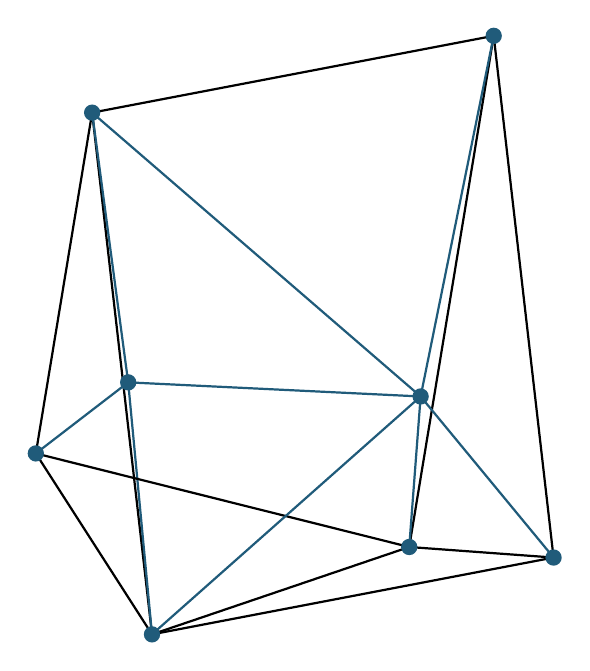
\begin{tikzpicture}[x  = {(0.9cm,-0.076cm)},
                    y  = {(-0.06cm,0.95cm)},
                    z  = {(-0.44cm,-0.29cm)},
                    scale = 2.5451,
                    color = {lightgray}]


  % DEF COORDINATES
  \coordinate (v0_piece3) at (0.178555, -0.726157, 1.79279);
  \coordinate (v1_piece3) at (-0.713713, 1.49968, 0.342827);
  \coordinate (v2_piece3) at (-0.621412, 0.0826052, 0.316224);
  \coordinate (v3_piece3) at (-1.42591, -0.512871, -0.200909);
  \coordinate (v4_piece3) at (1.78302, -0.588148, 0.50275);
  \coordinate (v5_piece3) at (-0.177542, -1.38114, -1.76282);
  \coordinate (v6_piece3) at (0.890748, 1.63769, -0.947213);
  \coordinate (v7_piece3) at (0.667593, -0.0886834, -0.339797);


  % VERTEXCOLOR
  \definecolor{vertexcolor_piece3}{rgb}{ 0.1255 0.3569 0.4784 }

  % DEF VERTEXSTYLES
  \tikzstyle{vertexstyle_piece3} = [circle, scale=0.625pt, fill=vertexcolor_piece3,]

  % EDGECOLOR
  \definecolor{edgecolor_piece3_0}{rgb}{ 0 0 0 }
  \definecolor{edgecolor_piece3_1}{rgb}{ 0.1255 0.3569 0.4784 }
  \tikzstyle{edgestyle_piece3_1_0} = [thick, color=edgecolor_piece3_0,]
  \tikzstyle{edgestyle_piece3_2_0} = [thick, color=edgecolor_piece3_1,]
  \tikzstyle{edgestyle_piece3_2_1} = [thick, color=edgecolor_piece3_1,]
  \tikzstyle{edgestyle_piece3_3_0} = [thick, color=edgecolor_piece3_0,]
  \tikzstyle{edgestyle_piece3_3_1} = [thick, color=edgecolor_piece3_0,]
  \tikzstyle{edgestyle_piece3_3_2} = [thick, color=edgecolor_piece3_1,]
  \tikzstyle{edgestyle_piece3_4_0} = [thick, color=edgecolor_piece3_0,]
  \tikzstyle{edgestyle_piece3_5_0} = [thick, color=edgecolor_piece3_0,]
  \tikzstyle{edgestyle_piece3_5_3} = [thick, color=edgecolor_piece3_0,]
  \tikzstyle{edgestyle_piece3_5_4} = [thick, color=edgecolor_piece3_0,]
  \tikzstyle{edgestyle_piece3_6_1} = [thick, color=edgecolor_piece3_0,]
  \tikzstyle{edgestyle_piece3_6_4} = [thick, color=edgecolor_piece3_0,]
  \tikzstyle{edgestyle_piece3_6_5} = [thick, color=edgecolor_piece3_0,]
  \tikzstyle{edgestyle_piece3_7_0} = [thick, color=edgecolor_piece3_1,]
  \tikzstyle{edgestyle_piece3_7_1} = [thick, color=edgecolor_piece3_1,]
  \tikzstyle{edgestyle_piece3_7_2} = [thick, color=edgecolor_piece3_1,]
  \tikzstyle{edgestyle_piece3_7_4} = [thick, color=edgecolor_piece3_1,]
  \tikzstyle{edgestyle_piece3_7_5} = [thick, color=edgecolor_piece3_1,]
  \tikzstyle{edgestyle_piece3_7_6} = [thick, color=edgecolor_piece3_1,]

  % EDGES

  \foreach \i/\k in {1/0,2/0,2/1,3/0,3/1,3/2,4/0,5/0,5/3,5/4,6/1,6/4,6/5,7/0,7/1,7/2,7/4,7/5,7/6} {
   \draw[edgestyle_piece3_\i_\k] (v\i_piece3) -- (v\k_piece3);
  }


  % POINTS
  \foreach \i in {0,4,1,2,3,7,6,5} {
    \node at (v\i_piece3) [vertexstyle_piece3] {};
  }


\end{tikzpicture}
\end{minipage}\par\vspace{3mm}
{\color{muted}In \(P_{15}\).}
\end{atlaspanel}\end{minipage}
\hfill
\begin{minipage}[t]{.323\textwidth}\begin{atlaspanel}
{\Large\bfseries \(\mathrm{U}^{4}_{8,8}\)}\hspace{3mm}{\normalsize\color{muted}unrecognized}\hfill{\normalsize\(f=(8,19,19,8)\)}\par\vspace{3mm}
\begin{minipage}[c][8.0cm][c]{\linewidth}\centering
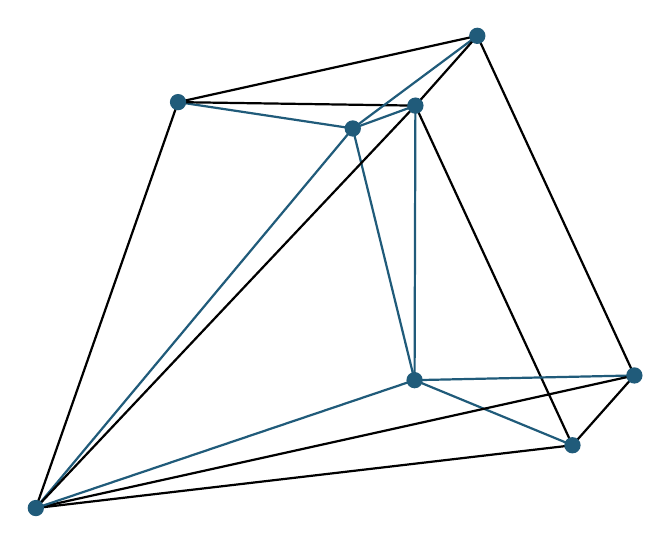
\begin{tikzpicture}[x  = {(0.9cm,-0.076cm)},
                    y  = {(-0.06cm,0.95cm)},
                    z  = {(-0.44cm,-0.29cm)},
                    scale = 2.3441,
                    color = {lightgray}]


  % DEF COORDINATES
  \coordinate (v0_piece4) at (-0.199501, 0.641788, -0.126408);
  \coordinate (v1_piece4) at (-0.674339, 0.219714, -1.81119);
  \coordinate (v2_piece4) at (-0.898465, 0.943599, 0.553645);
  \coordinate (v3_piece4) at (0.786402, 1.36619, 0.25804);
  \coordinate (v4_piece4) at (0.448906, -1.44641, -1.21998);
  \coordinate (v5_piece4) at (1.90965, -0.299926, 0.84925);
  \coordinate (v6_piece4) at (0.21156, -0.681032, 0.133801);
  \coordinate (v7_piece4) at (-1.46009, -1.14512, 1.44046);


  % VERTEXCOLOR
  \definecolor{vertexcolor_piece4}{rgb}{ 0.1255 0.3569 0.4784 }

  % DEF VERTEXSTYLES
  \tikzstyle{vertexstyle_piece4} = [circle, scale=0.625pt, fill=vertexcolor_piece4,]

  % EDGECOLOR
  \definecolor{edgecolor_piece4_0}{rgb}{ 0 0 0 }
  \definecolor{edgecolor_piece4_1}{rgb}{ 0.1255 0.3569 0.4784 }
  \tikzstyle{edgestyle_piece4_1_0} = [thick, color=edgecolor_piece4_1,]
  \tikzstyle{edgestyle_piece4_2_0} = [thick, color=edgecolor_piece4_1,]
  \tikzstyle{edgestyle_piece4_2_1} = [thick, color=edgecolor_piece4_0,]
  \tikzstyle{edgestyle_piece4_3_0} = [thick, color=edgecolor_piece4_1,]
  \tikzstyle{edgestyle_piece4_3_1} = [thick, color=edgecolor_piece4_0,]
  \tikzstyle{edgestyle_piece4_3_2} = [thick, color=edgecolor_piece4_0,]
  \tikzstyle{edgestyle_piece4_4_1} = [thick, color=edgecolor_piece4_0,]
  \tikzstyle{edgestyle_piece4_5_3} = [thick, color=edgecolor_piece4_0,]
  \tikzstyle{edgestyle_piece4_5_4} = [thick, color=edgecolor_piece4_0,]
  \tikzstyle{edgestyle_piece4_6_0} = [thick, color=edgecolor_piece4_1,]
  \tikzstyle{edgestyle_piece4_6_1} = [thick, color=edgecolor_piece4_1,]
  \tikzstyle{edgestyle_piece4_6_4} = [thick, color=edgecolor_piece4_1,]
  \tikzstyle{edgestyle_piece4_6_5} = [thick, color=edgecolor_piece4_1,]
  \tikzstyle{edgestyle_piece4_7_0} = [thick, color=edgecolor_piece4_1,]
  \tikzstyle{edgestyle_piece4_7_1} = [thick, color=edgecolor_piece4_0,]
  \tikzstyle{edgestyle_piece4_7_2} = [thick, color=edgecolor_piece4_0,]
  \tikzstyle{edgestyle_piece4_7_4} = [thick, color=edgecolor_piece4_0,]
  \tikzstyle{edgestyle_piece4_7_5} = [thick, color=edgecolor_piece4_0,]
  \tikzstyle{edgestyle_piece4_7_6} = [thick, color=edgecolor_piece4_1,]

  % EDGES

  \foreach \i/\k in {1/0,2/0,2/1,3/0,3/1,3/2,4/1,5/3,5/4,6/0,6/1,6/4,6/5,7/0,7/1,7/2,7/4,7/5,7/6} {
   \draw[edgestyle_piece4_\i_\k] (v\i_piece4) -- (v\k_piece4);
  }


  % POINTS
  \foreach \i in {7,5,2,3,6,0,4,1} {
    \node at (v\i_piece4) [vertexstyle_piece4] {};
  }


\end{tikzpicture}
\end{minipage}\par\vspace{3mm}
{\color{muted}In \(P_{16}\).}
\end{atlaspanel}\end{minipage}
\hfill
\begin{minipage}[t]{.323\textwidth}\begin{atlaspanel}
{\Large\bfseries \(\mathrm{U}^{4}_{9,8}\)}\hspace{3mm}{\normalsize\color{muted}unrecognized}\hfill{\normalsize\(f=(9,21,20,8)\)}\par\vspace{3mm}
\begin{minipage}[c][8.0cm][c]{\linewidth}\centering
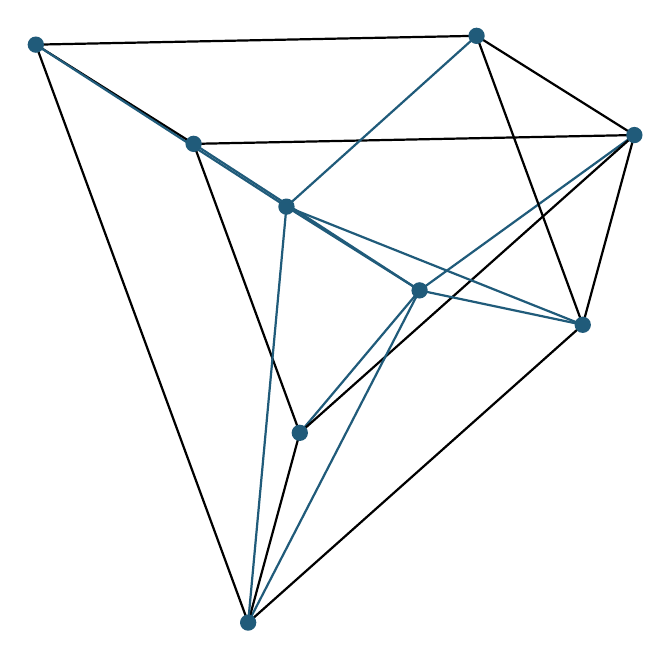
\begin{tikzpicture}[x  = {(0.9cm,-0.076cm)},
                    y  = {(-0.06cm,0.95cm)},
                    z  = {(-0.44cm,-0.29cm)},
                    scale = 2.3078,
                    color = {lightgray}]


  % DEF COORDINATES
  \coordinate (v0_piece5) at (-0.000226656, -0.476666, -0.767566);
  \coordinate (v1_piece5) at (0.94225, 0.23722, -1.62292);
  \coordinate (v2_piece5) at (-0.707084, -1.30781, -0.602139);
  \coordinate (v3_piece5) at (-1.41496, 0.209302, -0.929312);
  \coordinate (v4_piece5) at (-0.000226656, 0.476714, 0.767287);
  \coordinate (v5_piece5) at (0.94225, 1.36715, 0.196164);
  \coordinate (v6_piece5) at (-1.41496, 1.33923, 0.889772);
  \coordinate (v7_piece5) at (1.65013, -0.149955, 0.523338);
  \coordinate (v8_piece5) at (0.000793295, -1.69498, 1.54412);


  % VERTEXCOLOR
  \definecolor{vertexcolor_piece5}{rgb}{ 0.1255 0.3569 0.4784 }

  % DEF VERTEXSTYLES
  \tikzstyle{vertexstyle_piece5} = [circle, scale=0.625pt, fill=vertexcolor_piece5,]

  % EDGECOLOR
  \definecolor{edgecolor_piece5_0}{rgb}{ 0 0 0 }
  \definecolor{edgecolor_piece5_1}{rgb}{ 0.1255 0.3569 0.4784 }
  \tikzstyle{edgestyle_piece5_1_0} = [thick, color=edgecolor_piece5_1,]
  \tikzstyle{edgestyle_piece5_2_0} = [thick, color=edgecolor_piece5_1,]
  \tikzstyle{edgestyle_piece5_2_1} = [thick, color=edgecolor_piece5_0,]
  \tikzstyle{edgestyle_piece5_3_0} = [thick, color=edgecolor_piece5_1,]
  \tikzstyle{edgestyle_piece5_3_1} = [thick, color=edgecolor_piece5_0,]
  \tikzstyle{edgestyle_piece5_3_2} = [thick, color=edgecolor_piece5_0,]
  \tikzstyle{edgestyle_piece5_4_0} = [thick, color=edgecolor_piece5_1,]
  \tikzstyle{edgestyle_piece5_5_1} = [thick, color=edgecolor_piece5_0,]
  \tikzstyle{edgestyle_piece5_5_4} = [thick, color=edgecolor_piece5_1,]
  \tikzstyle{edgestyle_piece5_6_3} = [thick, color=edgecolor_piece5_0,]
  \tikzstyle{edgestyle_piece5_6_4} = [thick, color=edgecolor_piece5_1,]
  \tikzstyle{edgestyle_piece5_6_5} = [thick, color=edgecolor_piece5_0,]
  \tikzstyle{edgestyle_piece5_7_0} = [thick, color=edgecolor_piece5_1,]
  \tikzstyle{edgestyle_piece5_7_1} = [thick, color=edgecolor_piece5_0,]
  \tikzstyle{edgestyle_piece5_7_4} = [thick, color=edgecolor_piece5_1,]
  \tikzstyle{edgestyle_piece5_7_5} = [thick, color=edgecolor_piece5_0,]
  \tikzstyle{edgestyle_piece5_8_0} = [thick, color=edgecolor_piece5_1,]
  \tikzstyle{edgestyle_piece5_8_2} = [thick, color=edgecolor_piece5_0,]
  \tikzstyle{edgestyle_piece5_8_4} = [thick, color=edgecolor_piece5_1,]
  \tikzstyle{edgestyle_piece5_8_6} = [thick, color=edgecolor_piece5_0,]
  \tikzstyle{edgestyle_piece5_8_7} = [thick, color=edgecolor_piece5_0,]

  % EDGES

  \foreach \i/\k in {1/0,2/0,2/1,3/0,3/1,3/2,4/0,5/1,5/4,6/3,6/4,6/5,7/0,7/1,7/4,7/5,8/0,8/2,8/4,8/6,8/7} {
   \draw[edgestyle_piece5_\i_\k] (v\i_piece5) -- (v\k_piece5);
  }


  % POINTS
  \foreach \i in {8,6,4,7,5,2,0,3,1} {
    \node at (v\i_piece5) [vertexstyle_piece5] {};
  }


\end{tikzpicture}
\end{minipage}\par\vspace{3mm}
{\color{muted}In \(P_{17}\).}
\end{atlaspanel}\end{minipage}
\par\vspace{4mm}
\begin{atlaspanel}
{\Large\bfseries Notation}\par\vspace{2mm}
\(Q\ast\Delta_{k-1}\) is the join of \(Q\) with a \((k-1)\)-simplex, that is,
the \(k\)-fold pyramid over \(Q\), and \(\mathrm{Wed}(Q;\,F)\) is the wedge
over \(Q\) at its face \(F\).  \(\Delta_d\) is the \(d\)-simplex, so \(\Delta_0\)
is a point, \(\Delta_1\) a segment and \(\Delta_2\) a triangle;
\(\square\) is a quadrilateral, \(\mathrm{M}(d,n)\) the \(d\)-dimensional
multiplex with \(n+1\) vertices, \(\mathrm{AP}_4\) the square antiprism, and
\(\mathrm{U}^d_{v,f}\) an unrecognized \(d\)-polytope with \(v\) vertices and
\(f\) facets.  The smallest piece of a type is its innermost base, such as
\(\mathrm{M}(3,5)\) in \(\mathrm{M}(3,5)\ast\Delta_1\).  Under each drawing
are the polytopes \(P_O\) that have this smallest piece.
In the solids, triangles are blue and quadrilaterals orange.  A 4-polytope is
drawn as its Schlegel diagram in a facet with the most vertices, whose edges
are black.
\end{atlaspanel}
\clearpage
\begin{atlaspanel}[top=1mm,bottom=2mm]
\AtlasSupportOrbitSplit{%
\vspace*{-3mm}\mbox{{\LARGE\bfseries Triangle orbit 1}\hspace{3mm}\raisebox{.8mm}[0pt][0pt]{{\fontsize{16}{18}\selectfont\color{muted}size 6}}}%
}{%
\vspace*{-3mm}{\fontsize{13}{16}\selectfont{\color{muted}\(\mathbb{Q}\) and \(\mathbb{F}_2\)}\quad{\color{muted}\(\underline{\{7,\,18,\,41\}}\), \(\{6,\,18,\,40\}\), \(\{11,\,12,\,35\}\), \(\{6,\,35,\,40\}\), \(\{11,\,12,\,36\}\), \(\{7,\,36,\,41\}\)}\rule[-3mm]{0pt}{3mm}}%
}%
\end{atlaspanel}\vspace{2mm}
\begin{center}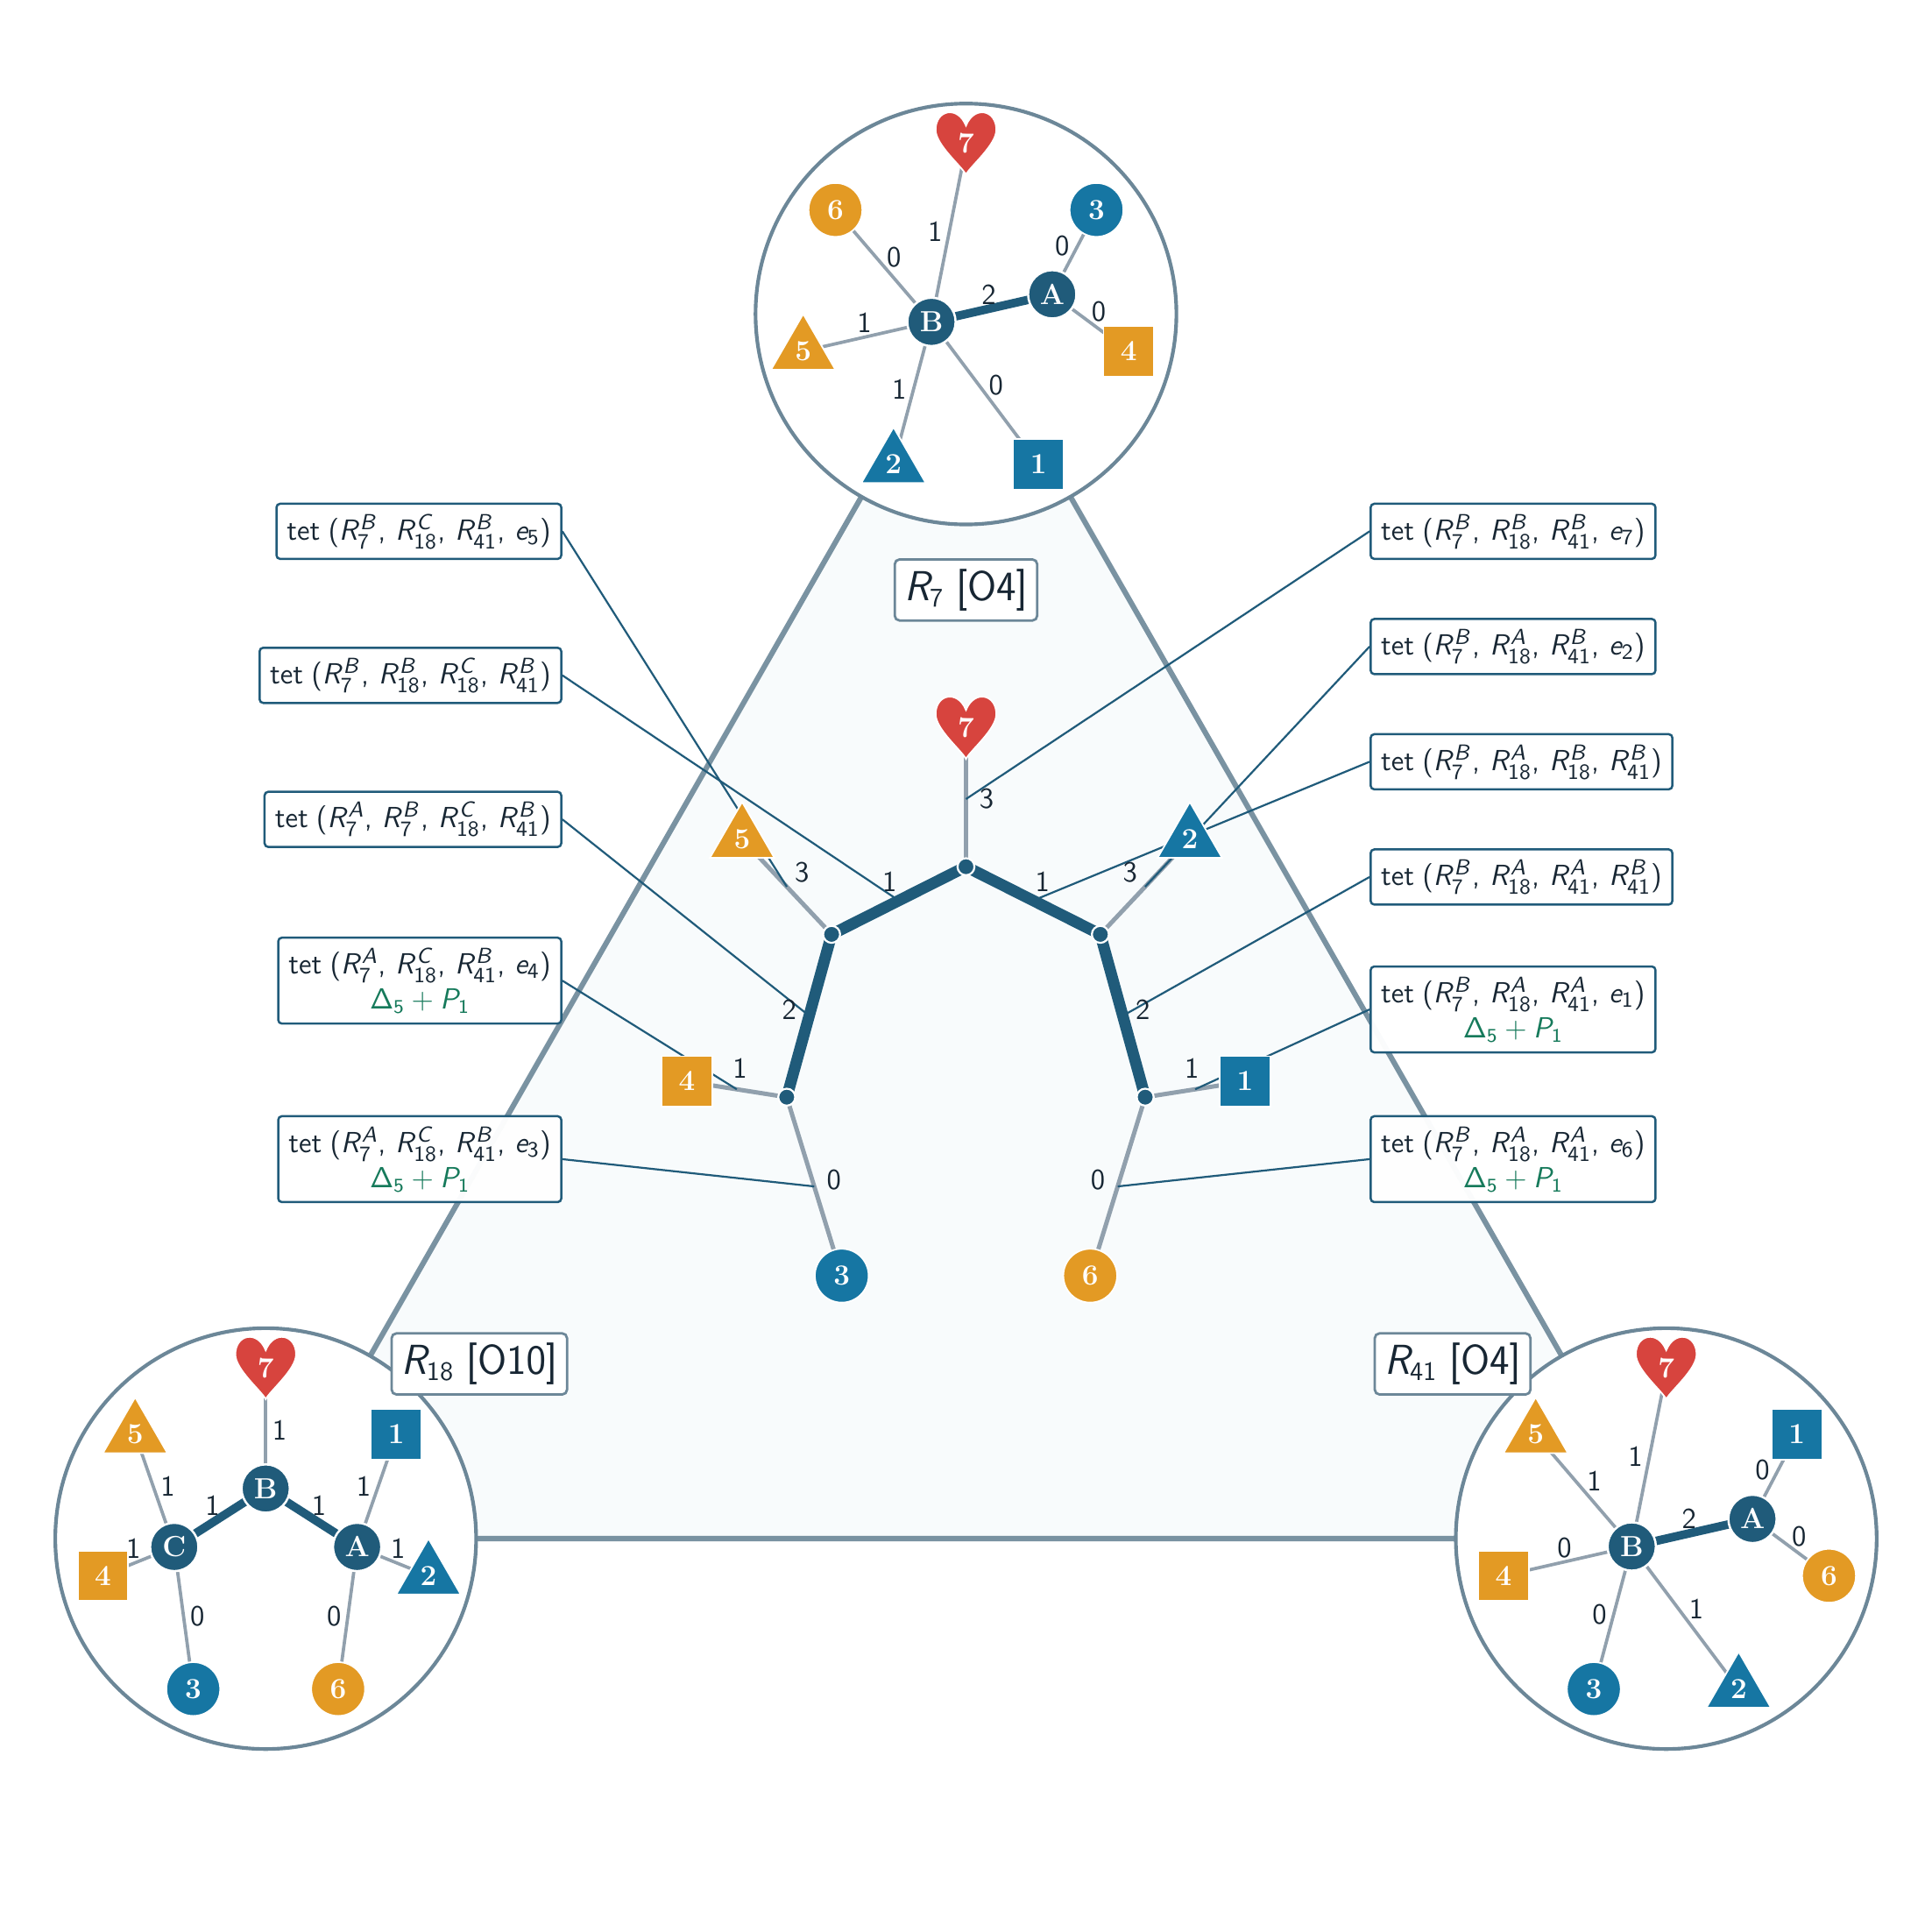
\begin{tikzpicture}[x=1cm,y=1cm]
\path[use as bounding box] (-13.65,-13.65) rectangle (13.65,13.65);
\path[support cell] (0.00000,9.45000)--(-10.15000,-8.30000)--(10.15000,-8.30000)--cycle;
\path[vertex disc] (0.00000,9.45000) circle[radius=3.05000cm];
\path[vertex disc] (-10.15000,-8.30000) circle[radius=3.05000cm];
\path[vertex disc] (10.15000,-8.30000) circle[radius=3.05000cm];
\coordinate (corner-1-v1) at (1.05000,7.26966);
\coordinate (corner-1-v2) at (-1.05000,7.26966);
\coordinate (corner-1-v3) at (1.89203,10.95885);
\coordinate (corner-1-v4) at (2.35933,8.91150);
\coordinate (corner-1-v5) at (-2.35933,8.91150);
\coordinate (corner-1-v6) at (-1.89203,10.95885);
\coordinate (corner-1-v7) at (0.00000,11.87000);
\coordinate (corner-1-v8) at (1.25040,9.73540);
\coordinate (corner-1-v9) at (-0.50016,9.33584);
\draw[internal edge] (corner-1-v8)--node[mini length,pos=0.5] {\(2\)}(corner-1-v9);
\draw[pendant edge] (corner-1-v1)--node[mini length,pos=0.5] {\(0\)}(corner-1-v9);
\draw[pendant edge] (corner-1-v2)--node[mini length,pos=0.5] {\(1\)}(corner-1-v9);
\draw[pendant edge] (corner-1-v3)--node[mini length,pos=0.5] {\(0\)}(corner-1-v8);
\draw[pendant edge] (corner-1-v4)--node[mini length,pos=0.5] {\(0\)}(corner-1-v8);
\draw[pendant edge] (corner-1-v5)--node[mini length,pos=0.5] {\(1\)}(corner-1-v9);
\draw[pendant edge] (corner-1-v6)--node[mini length,pos=0.5] {\(0\)}(corner-1-v9);
\draw[pendant edge] (corner-1-v7)--node[mini length,pos=0.5] {\(1\)}(corner-1-v9);
\node[lettered vertex] at (corner-1-v8) {A};
\node[lettered vertex] at (corner-1-v9) {B};
\taxonone{corner-1-v1}
\taxontwo{corner-1-v2}
\taxonthree{corner-1-v3}
\taxonfour{corner-1-v4}
\taxonfive{corner-1-v5}
\taxonsix{corner-1-v6}
\taxonseven{corner-1-v7}
\node[ray title] at (0.00000,5.45000) {\(R_{7}\;[\mathrm{O}4]\)};
\coordinate (corner-2-v1) at (-8.25797,-6.79115);
\coordinate (corner-2-v2) at (-7.79067,-8.83850);
\coordinate (corner-2-v3) at (-11.20000,-10.48034);
\coordinate (corner-2-v4) at (-12.50933,-8.83850);
\coordinate (corner-2-v5) at (-12.04203,-6.79115);
\coordinate (corner-2-v6) at (-9.10000,-10.48034);
\coordinate (corner-2-v7) at (-10.15000,-5.88000);
\coordinate (corner-2-v8) at (-8.82466,-8.42100);
\coordinate (corner-2-v9) at (-10.15000,-7.57400);
\coordinate (corner-2-v10) at (-11.47534,-8.42100);
\draw[internal edge] (corner-2-v8)--node[mini length,pos=0.5] {\(1\)}(corner-2-v9);
\draw[internal edge] (corner-2-v9)--node[mini length,pos=0.5] {\(1\)}(corner-2-v10);
\draw[pendant edge] (corner-2-v1)--node[mini length,pos=0.5] {\(1\)}(corner-2-v8);
\draw[pendant edge] (corner-2-v2)--node[mini length,pos=0.5] {\(1\)}(corner-2-v8);
\draw[pendant edge] (corner-2-v3)--node[mini length,pos=0.5] {\(0\)}(corner-2-v10);
\draw[pendant edge] (corner-2-v4)--node[mini length,pos=0.5] {\(1\)}(corner-2-v10);
\draw[pendant edge] (corner-2-v5)--node[mini length,pos=0.5] {\(1\)}(corner-2-v10);
\draw[pendant edge] (corner-2-v6)--node[mini length,pos=0.5] {\(0\)}(corner-2-v8);
\draw[pendant edge] (corner-2-v7)--node[mini length,pos=0.5] {\(1\)}(corner-2-v9);
\node[lettered vertex] at (corner-2-v8) {A};
\node[lettered vertex] at (corner-2-v9) {B};
\node[lettered vertex] at (corner-2-v10) {C};
\taxonone{corner-2-v1}
\taxontwo{corner-2-v2}
\taxonthree{corner-2-v3}
\taxonfour{corner-2-v4}
\taxonfive{corner-2-v5}
\taxonsix{corner-2-v6}
\taxonseven{corner-2-v7}
\node[ray title] at (-7.05349,-5.76788) {\(R_{18}\;[\mathrm{O}10]\)};
\coordinate (corner-3-v1) at (12.04203,-6.79115);
\coordinate (corner-3-v2) at (11.20000,-10.48034);
\coordinate (corner-3-v3) at (9.10000,-10.48034);
\coordinate (corner-3-v4) at (7.79067,-8.83850);
\coordinate (corner-3-v5) at (8.25797,-6.79115);
\coordinate (corner-3-v6) at (12.50933,-8.83850);
\coordinate (corner-3-v7) at (10.15000,-5.88000);
\coordinate (corner-3-v8) at (11.40040,-8.01460);
\coordinate (corner-3-v9) at (9.64984,-8.41416);
\draw[internal edge] (corner-3-v8)--node[mini length,pos=0.5] {\(2\)}(corner-3-v9);
\draw[pendant edge] (corner-3-v1)--node[mini length,pos=0.5] {\(0\)}(corner-3-v8);
\draw[pendant edge] (corner-3-v2)--node[mini length,pos=0.5] {\(1\)}(corner-3-v9);
\draw[pendant edge] (corner-3-v3)--node[mini length,pos=0.5] {\(0\)}(corner-3-v9);
\draw[pendant edge] (corner-3-v4)--node[mini length,pos=0.5] {\(0\)}(corner-3-v9);
\draw[pendant edge] (corner-3-v5)--node[mini length,pos=0.5] {\(1\)}(corner-3-v9);
\draw[pendant edge] (corner-3-v6)--node[mini length,pos=0.5] {\(0\)}(corner-3-v8);
\draw[pendant edge] (corner-3-v7)--node[mini length,pos=0.5] {\(1\)}(corner-3-v9);
\node[lettered vertex] at (corner-3-v8) {A};
\node[lettered vertex] at (corner-3-v9) {B};
\taxonone{corner-3-v1}
\taxontwo{corner-3-v2}
\taxonthree{corner-3-v3}
\taxonfour{corner-3-v4}
\taxonfive{corner-3-v5}
\taxonsix{corner-3-v6}
\taxonseven{corner-3-v7}
\node[ray title] at (7.05349,-5.76788) {\(R_{41}\;[\mathrm{O}4]\)};
\coordinate (central-v1) at (4.04595,-1.67346);
\coordinate (central-v2) at (3.24460,1.83748);
\coordinate (central-v3) at (-1.80062,-4.48902);
\coordinate (central-v4) at (-4.04595,-1.67346);
\coordinate (central-v5) at (-3.24460,1.83748);
\coordinate (central-v6) at (1.80062,-4.48902);
\coordinate (central-v7) at (0.00000,3.40000);
\coordinate (central-v8) at (2.59804,-1.90139);
\coordinate (central-v9) at (-2.59804,-1.90139);
\coordinate (central-v10) at (1.94755,0.45833);
\coordinate (central-v11) at (-1.94755,0.45833);
\coordinate (central-v12) at (0.00000,1.43889);
\draw[central internal edge] (central-v8)--(central-v10);
\draw[central internal edge] (central-v9)--(central-v11);
\draw[central internal edge] (central-v10)--(central-v12);
\draw[central internal edge] (central-v11)--(central-v12);
\draw[central pendant edge] (central-v1)--(central-v8);
\draw[central pendant edge] (central-v2)--(central-v10);
\draw[central pendant edge] (central-v3)--(central-v9);
\draw[central pendant edge] (central-v4)--(central-v9);
\draw[central pendant edge] (central-v5)--(central-v11);
\draw[central pendant edge] (central-v6)--(central-v8);
\draw[central pendant edge] (central-v7)--(central-v12);
\draw[edge leader] (-5.85000,6.30000)--(-2.59607,1.14791);
\draw[edge leader] (-5.85000,4.21250)--(-0.97377,0.94861);
\draw[edge leader] (-5.85000,2.12500)--(-2.27279,-0.72153);
\draw[edge leader] (-5.85000,-0.21250)--(-3.32199,-1.78742);
\draw[edge leader] (-5.85000,-2.80000)--(-2.19933,-3.19520);
\draw[edge leader] (5.85000,6.30000)--(0.00000,2.41944);
\draw[edge leader] (5.85000,4.63000)--(2.59607,1.14791);
\draw[edge leader] (5.85000,2.96000)--(0.97377,0.94861);
\draw[edge leader] (5.85000,1.29000)--(2.27279,-0.72153);
\draw[edge leader] (5.85000,-0.63000)--(3.32199,-1.78742);
\draw[edge leader] (5.85000,-2.80000)--(2.19933,-3.19520);
\node[internal vertex] at (central-v8) {};
\node[internal vertex] at (central-v9) {};
\node[internal vertex] at (central-v10) {};
\node[internal vertex] at (central-v11) {};
\node[internal vertex] at (central-v12) {};
\taxonone{central-v1}
\taxontwo{central-v2}
\taxonthree{central-v3}
\taxonfour{central-v4}
\taxonfive{central-v5}
\taxonsix{central-v6}
\taxonseven{central-v7}
\path (central-v8)--node[central length,pos=.50] {\(2\)}(central-v10);
\path (central-v9)--node[central length,pos=.50] {\(2\)}(central-v11);
\path (central-v10)--node[central length,pos=.50] {\(1\)}(central-v12);
\path (central-v11)--node[central length,pos=.50] {\(1\)}(central-v12);
\path (central-v1)--node[central length,pos=.50] {\(1\)}(central-v8);
\path (central-v2)--node[central length,pos=.50] {\(3\)}(central-v10);
\path (central-v3)--node[central length,pos=.50] {\(0\)}(central-v9);
\path (central-v4)--node[central length,pos=.50] {\(1\)}(central-v9);
\path (central-v5)--node[central length,pos=.50] {\(3\)}(central-v11);
\path (central-v6)--node[central length,pos=.50] {\(0\)}(central-v8);
\path (central-v7)--node[central length,pos=.50] {\(3\)}(central-v12);
\node[edge callout,anchor=east] (callout-1) at (-5.85000,6.30000) {\(\mathrm{tet}\;(R_{7}^{B},\,R_{18}^{C},\,R_{41}^{B},\,e_{5})\)};
\node[edge callout,anchor=east] (callout-2) at (-5.85000,4.21250) {\(\mathrm{tet}\;(R_{7}^{B},\,R_{18}^{B},\,R_{18}^{C},\,R_{41}^{B})\)};
\node[edge callout,anchor=east] (callout-3) at (-5.85000,2.12500) {\(\mathrm{tet}\;(R_{7}^{A},\,R_{7}^{B},\,R_{18}^{C},\,R_{41}^{B})\)};
\node[edge callout,anchor=east] (callout-4) at (-5.85000,-0.21250) {\(\mathrm{tet}\;(R_{7}^{A},\,R_{18}^{C},\,R_{41}^{B},\,e_{4})\)\\{\fontsize{12}{14}\selectfont\color{toricgreen}\(\Delta_{5}+P_{1}\)}};
\node[edge callout,anchor=east] (callout-5) at (-5.85000,-2.80000) {\(\mathrm{tet}\;(R_{7}^{A},\,R_{18}^{C},\,R_{41}^{B},\,e_{3})\)\\{\fontsize{12}{14}\selectfont\color{toricgreen}\(\Delta_{5}+P_{1}\)}};
\node[edge callout,anchor=west] (callout-6) at (5.85000,6.30000) {\(\mathrm{tet}\;(R_{7}^{B},\,R_{18}^{B},\,R_{41}^{B},\,e_{7})\)};
\node[edge callout,anchor=west] (callout-7) at (5.85000,4.63000) {\(\mathrm{tet}\;(R_{7}^{B},\,R_{18}^{A},\,R_{41}^{B},\,e_{2})\)};
\node[edge callout,anchor=west] (callout-8) at (5.85000,2.96000) {\(\mathrm{tet}\;(R_{7}^{B},\,R_{18}^{A},\,R_{18}^{B},\,R_{41}^{B})\)};
\node[edge callout,anchor=west] (callout-9) at (5.85000,1.29000) {\(\mathrm{tet}\;(R_{7}^{B},\,R_{18}^{A},\,R_{41}^{A},\,R_{41}^{B})\)};
\node[edge callout,anchor=west] (callout-10) at (5.85000,-0.63000) {\(\mathrm{tet}\;(R_{7}^{B},\,R_{18}^{A},\,R_{41}^{A},\,e_{1})\)\\{\fontsize{12}{14}\selectfont\color{toricgreen}\(\Delta_{5}+P_{1}\)}};
\node[edge callout,anchor=west] (callout-11) at (5.85000,-2.80000) {\(\mathrm{tet}\;(R_{7}^{B},\,R_{18}^{A},\,R_{41}^{A},\,e_{6})\)\\{\fontsize{12}{14}\selectfont\color{toricgreen}\(\Delta_{5}+P_{1}\)}};
\end{tikzpicture}\end{center}\vspace{-1mm}
\begin{atlasbox}\begin{atlaspanel}
\textcolor{toricgreen}{\bfseries PRIME TORIC}\quad \(P_{1}\):\enspace \(\Delta_{5}\)\quad \(f=(6,15,20,15,6)\)\quad 14 lattice points\\[1mm]\textcolor{bodyviolet}{\bfseries CHEVALLEY POLYTOPE}\quad \(P_{G_2/P_2,\,\varpi_2,\,s}\) with \(s=s_2s_1s_2s_1s_2\), unimodularly equivalent to the lecture hall simplex \(P_{(1,3,2,3,1)}\)
\end{atlaspanel}\end{atlasbox}
\clearpage
\begin{atlaspanel}[top=1mm,bottom=2mm]
\AtlasSupportOrbitSplit{%
\vspace*{-3mm}\mbox{{\LARGE\bfseries Triangle orbit 2}\hspace{3mm}\raisebox{.8mm}[0pt][0pt]{{\fontsize{16}{18}\selectfont\color{muted}size 6}}}%
}{%
\vspace*{-3mm}{\fontsize{13}{16}\selectfont{\color{muted}\(\mathbb{Q}\) and \(\mathbb{F}_2\)}\quad{\color{muted}\(\underline{\{6,\,11,\,35\}}\), \(\{7,\,12,\,36\}\), \(\{7,\,18,\,40\}\), \(\{6,\,18,\,41\}\), \(\{11,\,36,\,41\}\), \(\{12,\,35,\,40\}\)}\rule[-3mm]{0pt}{3mm}}%
}%
\end{atlaspanel}\vspace{2mm}
\begin{center}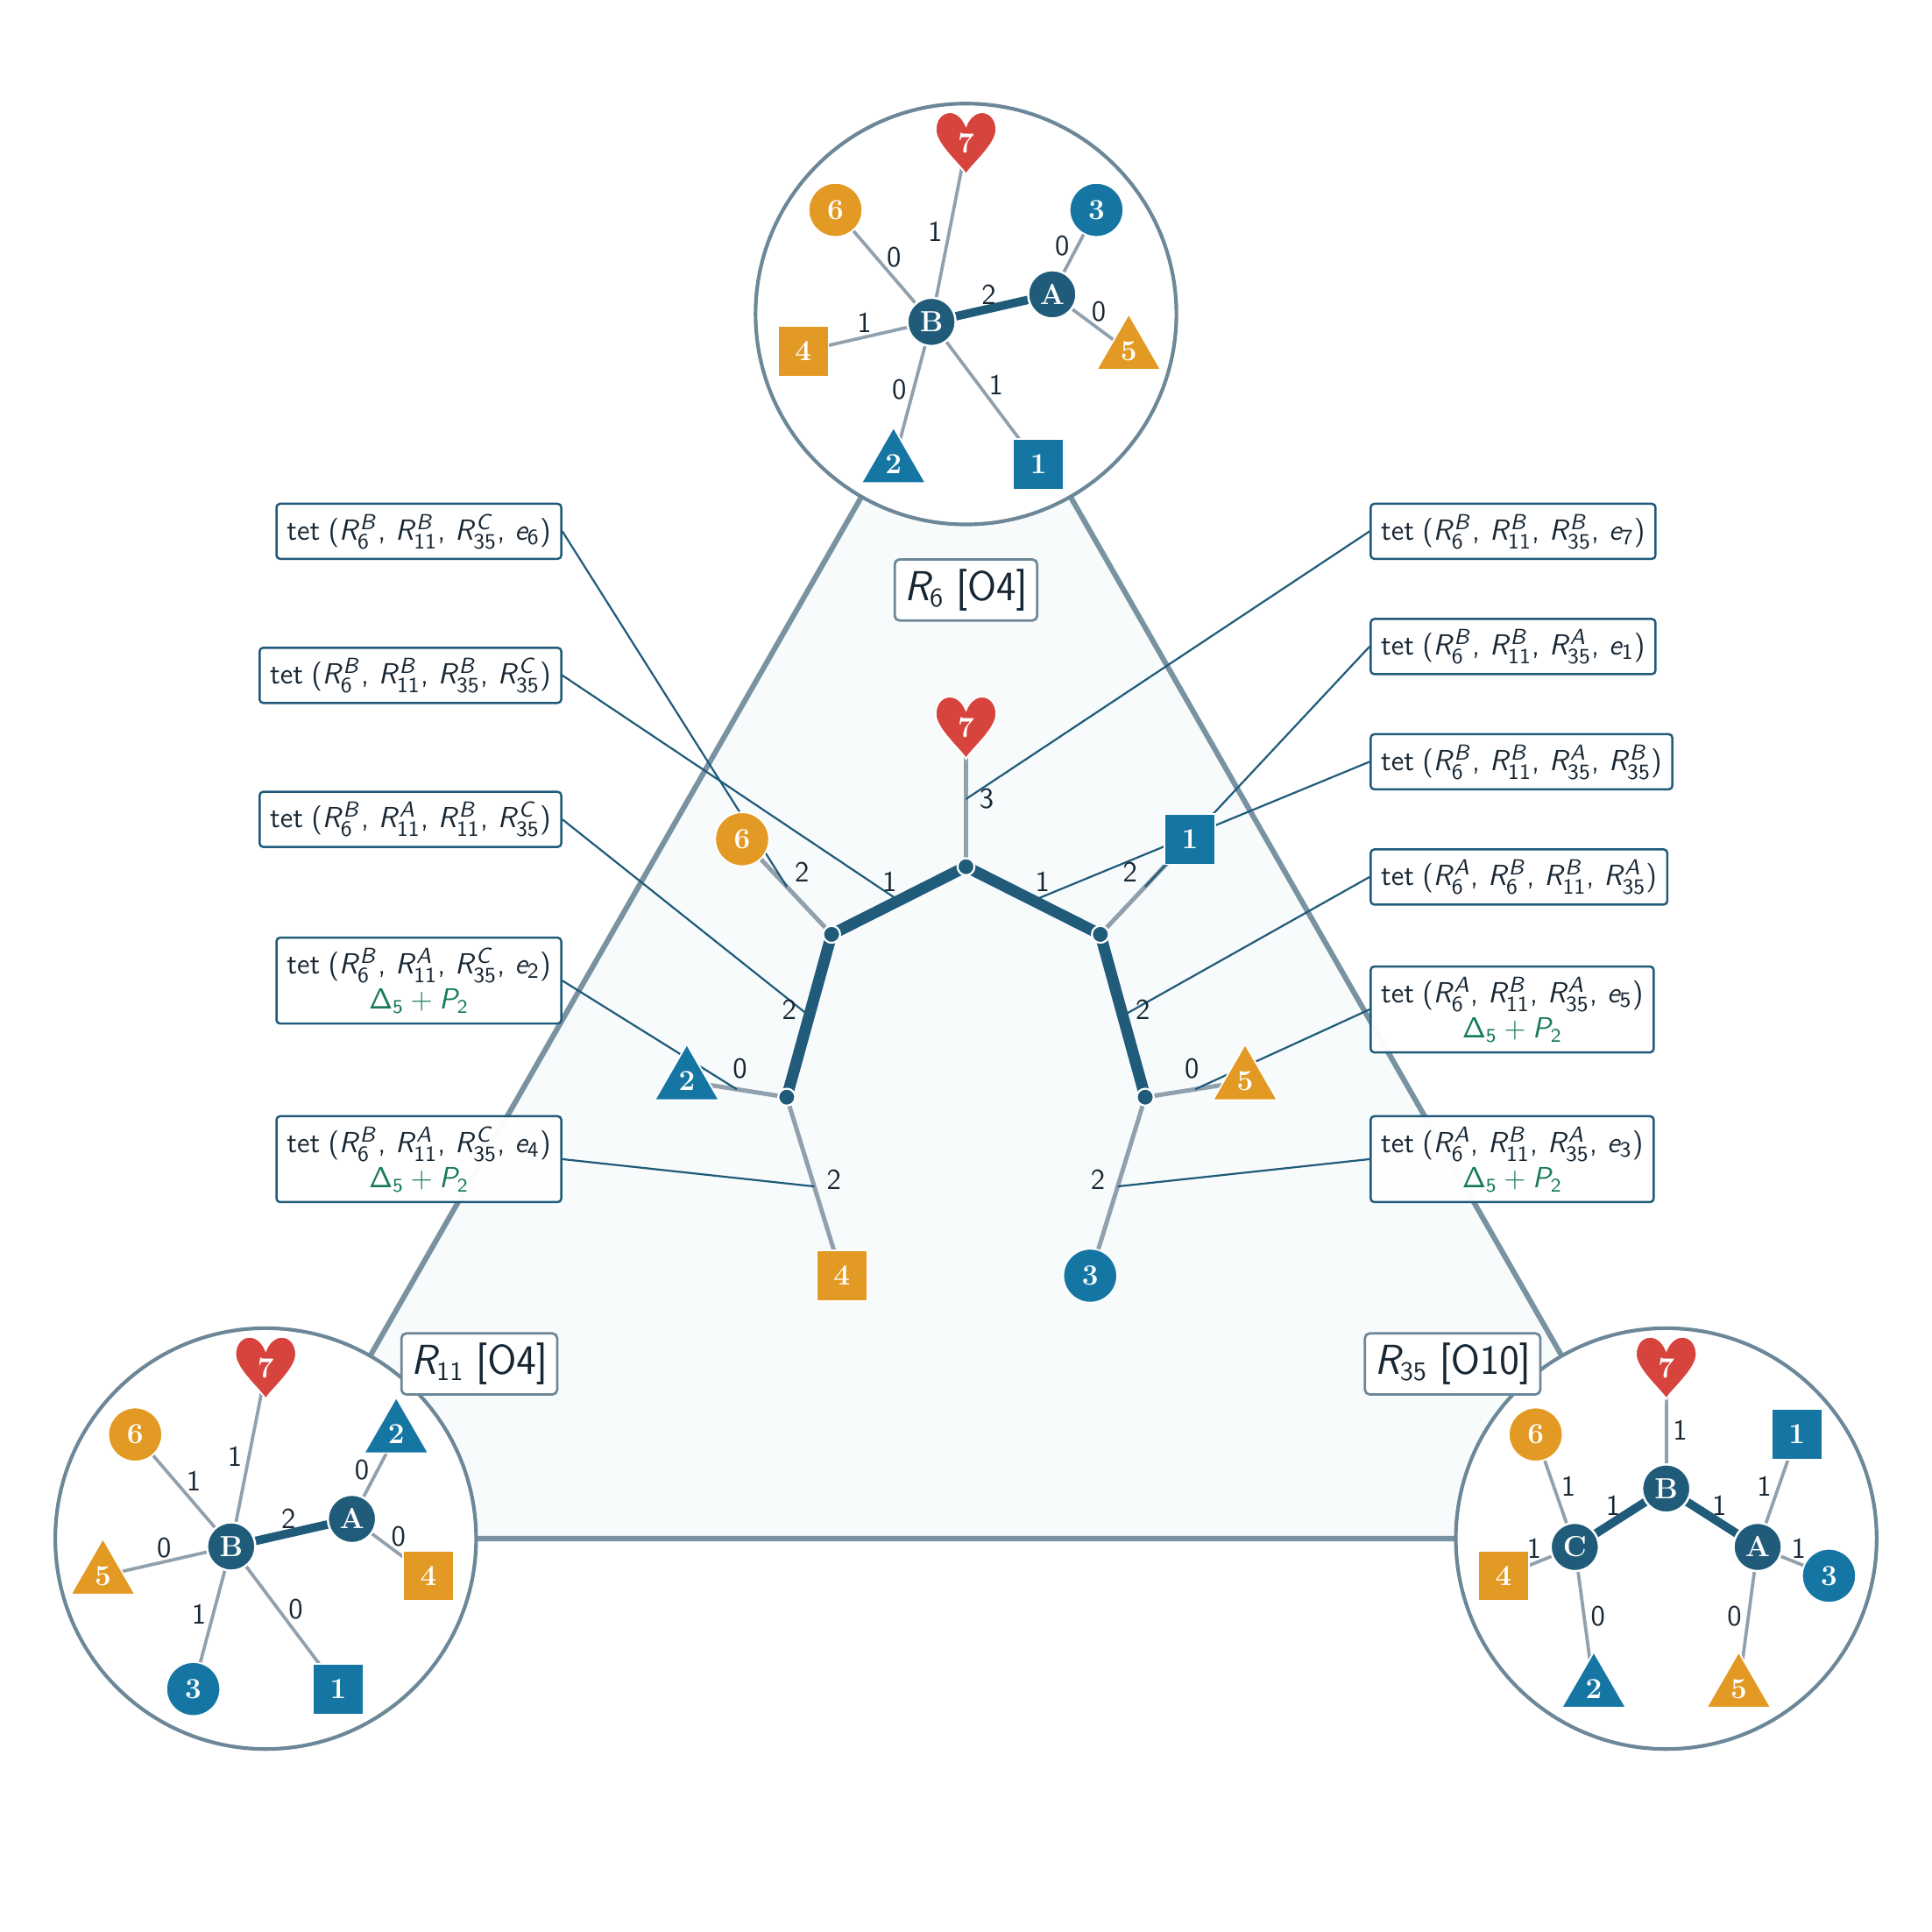
\begin{tikzpicture}[x=1cm,y=1cm]
\path[use as bounding box] (-13.65,-13.65) rectangle (13.65,13.65);
\path[support cell] (0.00000,9.45000)--(-10.15000,-8.30000)--(10.15000,-8.30000)--cycle;
\path[vertex disc] (0.00000,9.45000) circle[radius=3.05000cm];
\path[vertex disc] (-10.15000,-8.30000) circle[radius=3.05000cm];
\path[vertex disc] (10.15000,-8.30000) circle[radius=3.05000cm];
\coordinate (corner-1-v1) at (1.05000,7.26966);
\coordinate (corner-1-v2) at (-1.05000,7.26966);
\coordinate (corner-1-v3) at (1.89203,10.95885);
\coordinate (corner-1-v4) at (-2.35933,8.91150);
\coordinate (corner-1-v5) at (2.35933,8.91150);
\coordinate (corner-1-v6) at (-1.89203,10.95885);
\coordinate (corner-1-v7) at (0.00000,11.87000);
\coordinate (corner-1-v8) at (1.25040,9.73540);
\coordinate (corner-1-v9) at (-0.50016,9.33584);
\draw[internal edge] (corner-1-v8)--node[mini length,pos=0.5] {\(2\)}(corner-1-v9);
\draw[pendant edge] (corner-1-v1)--node[mini length,pos=0.5] {\(1\)}(corner-1-v9);
\draw[pendant edge] (corner-1-v2)--node[mini length,pos=0.5] {\(0\)}(corner-1-v9);
\draw[pendant edge] (corner-1-v3)--node[mini length,pos=0.5] {\(0\)}(corner-1-v8);
\draw[pendant edge] (corner-1-v4)--node[mini length,pos=0.5] {\(1\)}(corner-1-v9);
\draw[pendant edge] (corner-1-v5)--node[mini length,pos=0.5] {\(0\)}(corner-1-v8);
\draw[pendant edge] (corner-1-v6)--node[mini length,pos=0.5] {\(0\)}(corner-1-v9);
\draw[pendant edge] (corner-1-v7)--node[mini length,pos=0.5] {\(1\)}(corner-1-v9);
\node[lettered vertex] at (corner-1-v8) {A};
\node[lettered vertex] at (corner-1-v9) {B};
\taxonone{corner-1-v1}
\taxontwo{corner-1-v2}
\taxonthree{corner-1-v3}
\taxonfour{corner-1-v4}
\taxonfive{corner-1-v5}
\taxonsix{corner-1-v6}
\taxonseven{corner-1-v7}
\node[ray title] at (0.00000,5.45000) {\(R_{6}\;[\mathrm{O}4]\)};
\coordinate (corner-2-v1) at (-9.10000,-10.48034);
\coordinate (corner-2-v2) at (-8.25797,-6.79115);
\coordinate (corner-2-v3) at (-11.20000,-10.48034);
\coordinate (corner-2-v4) at (-7.79067,-8.83850);
\coordinate (corner-2-v5) at (-12.50933,-8.83850);
\coordinate (corner-2-v6) at (-12.04203,-6.79115);
\coordinate (corner-2-v7) at (-10.15000,-5.88000);
\coordinate (corner-2-v8) at (-8.89960,-8.01460);
\coordinate (corner-2-v9) at (-10.65016,-8.41416);
\draw[internal edge] (corner-2-v8)--node[mini length,pos=0.5] {\(2\)}(corner-2-v9);
\draw[pendant edge] (corner-2-v1)--node[mini length,pos=0.5] {\(0\)}(corner-2-v9);
\draw[pendant edge] (corner-2-v2)--node[mini length,pos=0.5] {\(0\)}(corner-2-v8);
\draw[pendant edge] (corner-2-v3)--node[mini length,pos=0.5] {\(1\)}(corner-2-v9);
\draw[pendant edge] (corner-2-v4)--node[mini length,pos=0.5] {\(0\)}(corner-2-v8);
\draw[pendant edge] (corner-2-v5)--node[mini length,pos=0.5] {\(0\)}(corner-2-v9);
\draw[pendant edge] (corner-2-v6)--node[mini length,pos=0.5] {\(1\)}(corner-2-v9);
\draw[pendant edge] (corner-2-v7)--node[mini length,pos=0.5] {\(1\)}(corner-2-v9);
\node[lettered vertex] at (corner-2-v8) {A};
\node[lettered vertex] at (corner-2-v9) {B};
\taxonone{corner-2-v1}
\taxontwo{corner-2-v2}
\taxonthree{corner-2-v3}
\taxonfour{corner-2-v4}
\taxonfive{corner-2-v5}
\taxonsix{corner-2-v6}
\taxonseven{corner-2-v7}
\node[ray title] at (-7.05349,-5.76788) {\(R_{11}\;[\mathrm{O}4]\)};
\coordinate (corner-3-v1) at (12.04203,-6.79115);
\coordinate (corner-3-v2) at (9.10000,-10.48034);
\coordinate (corner-3-v3) at (12.50933,-8.83850);
\coordinate (corner-3-v4) at (7.79067,-8.83850);
\coordinate (corner-3-v5) at (11.20000,-10.48034);
\coordinate (corner-3-v6) at (8.25797,-6.79115);
\coordinate (corner-3-v7) at (10.15000,-5.88000);
\coordinate (corner-3-v8) at (11.47534,-8.42100);
\coordinate (corner-3-v9) at (10.15000,-7.57400);
\coordinate (corner-3-v10) at (8.82466,-8.42100);
\draw[internal edge] (corner-3-v8)--node[mini length,pos=0.5] {\(1\)}(corner-3-v9);
\draw[internal edge] (corner-3-v9)--node[mini length,pos=0.5] {\(1\)}(corner-3-v10);
\draw[pendant edge] (corner-3-v1)--node[mini length,pos=0.5] {\(1\)}(corner-3-v8);
\draw[pendant edge] (corner-3-v2)--node[mini length,pos=0.5] {\(0\)}(corner-3-v10);
\draw[pendant edge] (corner-3-v3)--node[mini length,pos=0.5] {\(1\)}(corner-3-v8);
\draw[pendant edge] (corner-3-v4)--node[mini length,pos=0.5] {\(1\)}(corner-3-v10);
\draw[pendant edge] (corner-3-v5)--node[mini length,pos=0.5] {\(0\)}(corner-3-v8);
\draw[pendant edge] (corner-3-v6)--node[mini length,pos=0.5] {\(1\)}(corner-3-v10);
\draw[pendant edge] (corner-3-v7)--node[mini length,pos=0.5] {\(1\)}(corner-3-v9);
\node[lettered vertex] at (corner-3-v8) {A};
\node[lettered vertex] at (corner-3-v9) {B};
\node[lettered vertex] at (corner-3-v10) {C};
\taxonone{corner-3-v1}
\taxontwo{corner-3-v2}
\taxonthree{corner-3-v3}
\taxonfour{corner-3-v4}
\taxonfive{corner-3-v5}
\taxonsix{corner-3-v6}
\taxonseven{corner-3-v7}
\node[ray title] at (7.05349,-5.76788) {\(R_{35}\;[\mathrm{O}10]\)};
\coordinate (central-v1) at (3.24460,1.83748);
\coordinate (central-v2) at (-4.04595,-1.67346);
\coordinate (central-v3) at (1.80062,-4.48902);
\coordinate (central-v4) at (-1.80062,-4.48902);
\coordinate (central-v5) at (4.04595,-1.67346);
\coordinate (central-v6) at (-3.24460,1.83748);
\coordinate (central-v7) at (0.00000,3.40000);
\coordinate (central-v8) at (-2.59804,-1.90139);
\coordinate (central-v9) at (2.59804,-1.90139);
\coordinate (central-v10) at (1.94755,0.45833);
\coordinate (central-v11) at (-1.94755,0.45833);
\coordinate (central-v12) at (0.00000,1.43889);
\draw[central internal edge] (central-v8)--(central-v11);
\draw[central internal edge] (central-v9)--(central-v10);
\draw[central internal edge] (central-v10)--(central-v12);
\draw[central internal edge] (central-v11)--(central-v12);
\draw[central pendant edge] (central-v1)--(central-v10);
\draw[central pendant edge] (central-v2)--(central-v8);
\draw[central pendant edge] (central-v3)--(central-v9);
\draw[central pendant edge] (central-v4)--(central-v8);
\draw[central pendant edge] (central-v5)--(central-v9);
\draw[central pendant edge] (central-v6)--(central-v11);
\draw[central pendant edge] (central-v7)--(central-v12);
\draw[edge leader] (-5.85000,6.30000)--(-2.59607,1.14791);
\draw[edge leader] (-5.85000,4.21250)--(-0.97377,0.94861);
\draw[edge leader] (-5.85000,2.12500)--(-2.27279,-0.72153);
\draw[edge leader] (-5.85000,-0.21250)--(-3.32199,-1.78742);
\draw[edge leader] (-5.85000,-2.80000)--(-2.19933,-3.19520);
\draw[edge leader] (5.85000,6.30000)--(0.00000,2.41944);
\draw[edge leader] (5.85000,4.63000)--(2.59607,1.14791);
\draw[edge leader] (5.85000,2.96000)--(0.97377,0.94861);
\draw[edge leader] (5.85000,1.29000)--(2.27279,-0.72153);
\draw[edge leader] (5.85000,-0.63000)--(3.32199,-1.78742);
\draw[edge leader] (5.85000,-2.80000)--(2.19933,-3.19520);
\node[internal vertex] at (central-v8) {};
\node[internal vertex] at (central-v9) {};
\node[internal vertex] at (central-v10) {};
\node[internal vertex] at (central-v11) {};
\node[internal vertex] at (central-v12) {};
\taxonone{central-v1}
\taxontwo{central-v2}
\taxonthree{central-v3}
\taxonfour{central-v4}
\taxonfive{central-v5}
\taxonsix{central-v6}
\taxonseven{central-v7}
\path (central-v8)--node[central length,pos=.50] {\(2\)}(central-v11);
\path (central-v9)--node[central length,pos=.50] {\(2\)}(central-v10);
\path (central-v10)--node[central length,pos=.50] {\(1\)}(central-v12);
\path (central-v11)--node[central length,pos=.50] {\(1\)}(central-v12);
\path (central-v1)--node[central length,pos=.50] {\(2\)}(central-v10);
\path (central-v2)--node[central length,pos=.50] {\(0\)}(central-v8);
\path (central-v3)--node[central length,pos=.50] {\(2\)}(central-v9);
\path (central-v4)--node[central length,pos=.50] {\(2\)}(central-v8);
\path (central-v5)--node[central length,pos=.50] {\(0\)}(central-v9);
\path (central-v6)--node[central length,pos=.50] {\(2\)}(central-v11);
\path (central-v7)--node[central length,pos=.50] {\(3\)}(central-v12);
\node[edge callout,anchor=east] (callout-1) at (-5.85000,6.30000) {\(\mathrm{tet}\;(R_{6}^{B},\,R_{11}^{B},\,R_{35}^{C},\,e_{6})\)};
\node[edge callout,anchor=east] (callout-2) at (-5.85000,4.21250) {\(\mathrm{tet}\;(R_{6}^{B},\,R_{11}^{B},\,R_{35}^{B},\,R_{35}^{C})\)};
\node[edge callout,anchor=east] (callout-3) at (-5.85000,2.12500) {\(\mathrm{tet}\;(R_{6}^{B},\,R_{11}^{A},\,R_{11}^{B},\,R_{35}^{C})\)};
\node[edge callout,anchor=east] (callout-4) at (-5.85000,-0.21250) {\(\mathrm{tet}\;(R_{6}^{B},\,R_{11}^{A},\,R_{35}^{C},\,e_{2})\)\\{\fontsize{12}{14}\selectfont\color{toricgreen}\(\Delta_{5}+P_{2}\)}};
\node[edge callout,anchor=east] (callout-5) at (-5.85000,-2.80000) {\(\mathrm{tet}\;(R_{6}^{B},\,R_{11}^{A},\,R_{35}^{C},\,e_{4})\)\\{\fontsize{12}{14}\selectfont\color{toricgreen}\(\Delta_{5}+P_{2}\)}};
\node[edge callout,anchor=west] (callout-6) at (5.85000,6.30000) {\(\mathrm{tet}\;(R_{6}^{B},\,R_{11}^{B},\,R_{35}^{B},\,e_{7})\)};
\node[edge callout,anchor=west] (callout-7) at (5.85000,4.63000) {\(\mathrm{tet}\;(R_{6}^{B},\,R_{11}^{B},\,R_{35}^{A},\,e_{1})\)};
\node[edge callout,anchor=west] (callout-8) at (5.85000,2.96000) {\(\mathrm{tet}\;(R_{6}^{B},\,R_{11}^{B},\,R_{35}^{A},\,R_{35}^{B})\)};
\node[edge callout,anchor=west] (callout-9) at (5.85000,1.29000) {\(\mathrm{tet}\;(R_{6}^{A},\,R_{6}^{B},\,R_{11}^{B},\,R_{35}^{A})\)};
\node[edge callout,anchor=west] (callout-10) at (5.85000,-0.63000) {\(\mathrm{tet}\;(R_{6}^{A},\,R_{11}^{B},\,R_{35}^{A},\,e_{5})\)\\{\fontsize{12}{14}\selectfont\color{toricgreen}\(\Delta_{5}+P_{2}\)}};
\node[edge callout,anchor=west] (callout-11) at (5.85000,-2.80000) {\(\mathrm{tet}\;(R_{6}^{A},\,R_{11}^{B},\,R_{35}^{A},\,e_{3})\)\\{\fontsize{12}{14}\selectfont\color{toricgreen}\(\Delta_{5}+P_{2}\)}};
\end{tikzpicture}\end{center}\vspace{-1mm}
\begin{atlasbox}\begin{atlaspanel}
\textcolor{toricgreen}{\bfseries PRIME TORIC}\quad \(P_{2}\):\enspace \(\Delta_{5}\)\quad \(f=(6,15,20,15,6)\)\quad 16 lattice points
\end{atlaspanel}\end{atlasbox}
\clearpage
\begin{atlaspanel}[top=1mm,bottom=2mm]
\AtlasSupportOrbitSplit{%
\vspace*{-3mm}\mbox{{\LARGE\bfseries Triangle orbit 3}\hspace{3mm}\raisebox{.8mm}[0pt][0pt]{{\fontsize{16}{18}\selectfont\color{muted}size 12}}}%
}{%
\vspace*{-3mm}{\fontsize{13}{16}\selectfont{\color{muted}\(\mathbb{Q}\) and \(\mathbb{F}_2\)}\quad{\color{muted}\(\underline{\{2,\,7,\,13\}}\), \(\{2,\,6,\,13\}\), \(\{6,\,20,\,32\}\), \(\{17,\,28,\,40\}\), \(\{7,\,19,\,31\}\), \(\{17,\,28,\,41\}\), \(\{11,\,19,\,31\}\), \(\{12,\,20,\,32\}\), \(\{11,\,25,\,44\}\), \(\{12,\,26,\,45\}\), \(\{25,\,40,\,44\}\), \(\{26,\,41,\,45\}\)}\rule[-3mm]{0pt}{3mm}}%
}%
\end{atlaspanel}\vspace{2mm}
\begin{center}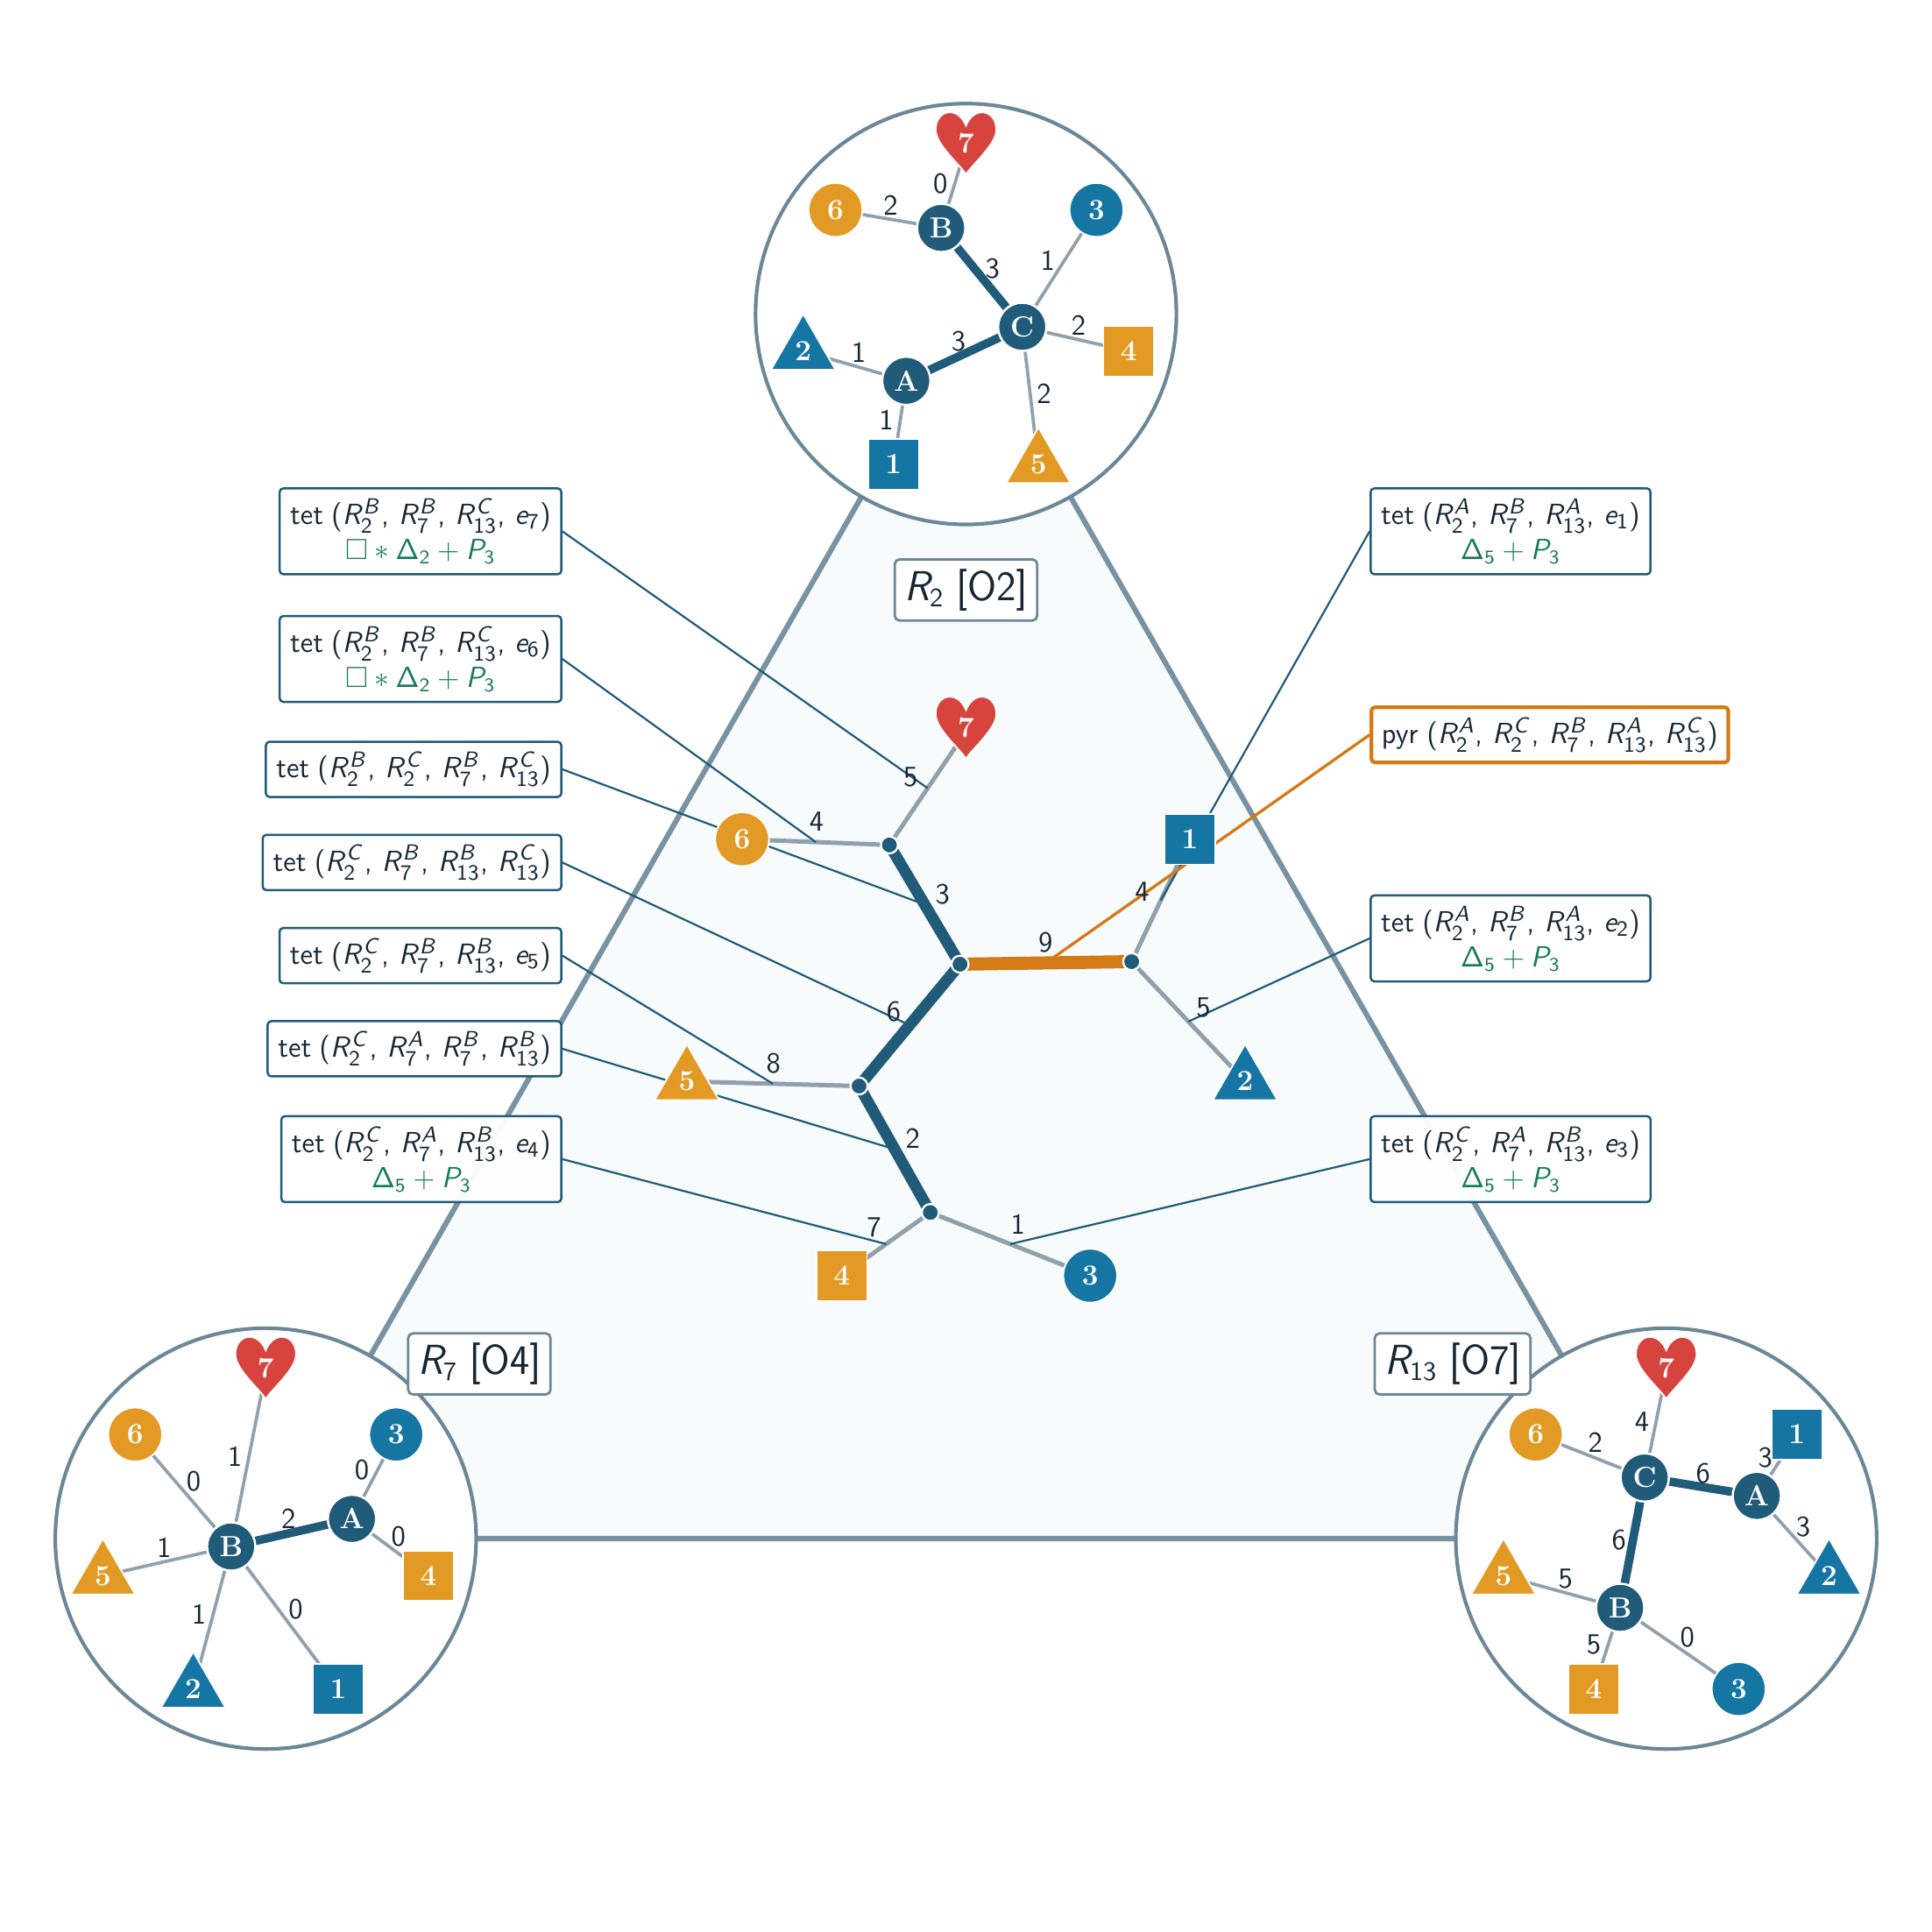
\begin{tikzpicture}[x=1cm,y=1cm]
\path[use as bounding box] (-13.65,-13.65) rectangle (13.65,13.65);
\path[support cell] (0.00000,9.45000)--(-10.15000,-8.30000)--(10.15000,-8.30000)--cycle;
\path[vertex disc] (0.00000,9.45000) circle[radius=3.05000cm];
\path[vertex disc] (-10.15000,-8.30000) circle[radius=3.05000cm];
\path[vertex disc] (10.15000,-8.30000) circle[radius=3.05000cm];
\coordinate (corner-1-v1) at (-1.05000,7.26966);
\coordinate (corner-1-v2) at (-2.35933,8.91150);
\coordinate (corner-1-v3) at (1.89203,10.95885);
\coordinate (corner-1-v4) at (2.35933,8.91150);
\coordinate (corner-1-v5) at (1.05000,7.26966);
\coordinate (corner-1-v6) at (-1.89203,10.95885);
\coordinate (corner-1-v7) at (0.00000,11.87000);
\coordinate (corner-1-v8) at (-0.86458,8.48167);
\coordinate (corner-1-v9) at (-0.35881,10.69756);
\coordinate (corner-1-v10) at (0.81559,9.26385);
\draw[internal edge] (corner-1-v8)--node[mini length,pos=0.5] {\(3\)}(corner-1-v10);
\draw[internal edge] (corner-1-v9)--node[mini length,pos=0.5] {\(3\)}(corner-1-v10);
\draw[pendant edge] (corner-1-v1)--node[mini length,pos=0.5] {\(1\)}(corner-1-v8);
\draw[pendant edge] (corner-1-v2)--node[mini length,pos=0.5] {\(1\)}(corner-1-v8);
\draw[pendant edge] (corner-1-v3)--node[mini length,pos=0.5] {\(1\)}(corner-1-v10);
\draw[pendant edge] (corner-1-v4)--node[mini length,pos=0.5] {\(2\)}(corner-1-v10);
\draw[pendant edge] (corner-1-v5)--node[mini length,pos=0.5] {\(2\)}(corner-1-v10);
\draw[pendant edge] (corner-1-v6)--node[mini length,pos=0.5] {\(2\)}(corner-1-v9);
\draw[pendant edge] (corner-1-v7)--node[mini length,pos=0.5] {\(0\)}(corner-1-v9);
\node[lettered vertex] at (corner-1-v8) {A};
\node[lettered vertex] at (corner-1-v9) {B};
\node[lettered vertex] at (corner-1-v10) {C};
\taxonone{corner-1-v1}
\taxontwo{corner-1-v2}
\taxonthree{corner-1-v3}
\taxonfour{corner-1-v4}
\taxonfive{corner-1-v5}
\taxonsix{corner-1-v6}
\taxonseven{corner-1-v7}
\node[ray title] at (0.00000,5.45000) {\(R_{2}\;[\mathrm{O}2]\)};
\coordinate (corner-2-v1) at (-9.10000,-10.48034);
\coordinate (corner-2-v2) at (-11.20000,-10.48034);
\coordinate (corner-2-v3) at (-8.25797,-6.79115);
\coordinate (corner-2-v4) at (-7.79067,-8.83850);
\coordinate (corner-2-v5) at (-12.50933,-8.83850);
\coordinate (corner-2-v6) at (-12.04203,-6.79115);
\coordinate (corner-2-v7) at (-10.15000,-5.88000);
\coordinate (corner-2-v8) at (-8.89960,-8.01460);
\coordinate (corner-2-v9) at (-10.65016,-8.41416);
\draw[internal edge] (corner-2-v8)--node[mini length,pos=0.5] {\(2\)}(corner-2-v9);
\draw[pendant edge] (corner-2-v1)--node[mini length,pos=0.5] {\(0\)}(corner-2-v9);
\draw[pendant edge] (corner-2-v2)--node[mini length,pos=0.5] {\(1\)}(corner-2-v9);
\draw[pendant edge] (corner-2-v3)--node[mini length,pos=0.5] {\(0\)}(corner-2-v8);
\draw[pendant edge] (corner-2-v4)--node[mini length,pos=0.5] {\(0\)}(corner-2-v8);
\draw[pendant edge] (corner-2-v5)--node[mini length,pos=0.5] {\(1\)}(corner-2-v9);
\draw[pendant edge] (corner-2-v6)--node[mini length,pos=0.5] {\(0\)}(corner-2-v9);
\draw[pendant edge] (corner-2-v7)--node[mini length,pos=0.5] {\(1\)}(corner-2-v9);
\node[lettered vertex] at (corner-2-v8) {A};
\node[lettered vertex] at (corner-2-v9) {B};
\taxonone{corner-2-v1}
\taxontwo{corner-2-v2}
\taxonthree{corner-2-v3}
\taxonfour{corner-2-v4}
\taxonfive{corner-2-v5}
\taxonsix{corner-2-v6}
\taxonseven{corner-2-v7}
\node[ray title] at (-7.05349,-5.76788) {\(R_{7}\;[\mathrm{O}4]\)};
\coordinate (corner-3-v1) at (12.04203,-6.79115);
\coordinate (corner-3-v2) at (12.50933,-8.83850);
\coordinate (corner-3-v3) at (11.20000,-10.48034);
\coordinate (corner-3-v4) at (9.10000,-10.48034);
\coordinate (corner-3-v5) at (7.79067,-8.83850);
\coordinate (corner-3-v6) at (8.25797,-6.79115);
\coordinate (corner-3-v7) at (10.15000,-5.88000);
\coordinate (corner-3-v8) at (11.46324,-7.68119);
\coordinate (corner-3-v9) at (9.48226,-9.30327);
\coordinate (corner-3-v10) at (9.83837,-7.41390);
\draw[internal edge] (corner-3-v8)--node[mini length,pos=0.5] {\(6\)}(corner-3-v10);
\draw[internal edge] (corner-3-v9)--node[mini length,pos=0.5] {\(6\)}(corner-3-v10);
\draw[pendant edge] (corner-3-v1)--node[mini length,pos=0.5] {\(3\)}(corner-3-v8);
\draw[pendant edge] (corner-3-v2)--node[mini length,pos=0.5] {\(3\)}(corner-3-v8);
\draw[pendant edge] (corner-3-v3)--node[mini length,pos=0.5] {\(0\)}(corner-3-v9);
\draw[pendant edge] (corner-3-v4)--node[mini length,pos=0.5] {\(5\)}(corner-3-v9);
\draw[pendant edge] (corner-3-v5)--node[mini length,pos=0.5] {\(5\)}(corner-3-v9);
\draw[pendant edge] (corner-3-v6)--node[mini length,pos=0.5] {\(2\)}(corner-3-v10);
\draw[pendant edge] (corner-3-v7)--node[mini length,pos=0.5] {\(4\)}(corner-3-v10);
\node[lettered vertex] at (corner-3-v8) {A};
\node[lettered vertex] at (corner-3-v9) {B};
\node[lettered vertex] at (corner-3-v10) {C};
\taxonone{corner-3-v1}
\taxontwo{corner-3-v2}
\taxonthree{corner-3-v3}
\taxonfour{corner-3-v4}
\taxonfive{corner-3-v5}
\taxonsix{corner-3-v6}
\taxonseven{corner-3-v7}
\node[ray title] at (7.05349,-5.76788) {\(R_{13}\;[\mathrm{O}7]\)};
\coordinate (central-v1) at (3.24460,1.83748);
\coordinate (central-v2) at (4.04595,-1.67346);
\coordinate (central-v3) at (1.80062,-4.48902);
\coordinate (central-v4) at (-1.80062,-4.48902);
\coordinate (central-v5) at (-4.04595,-1.67346);
\coordinate (central-v6) at (-3.24460,1.83748);
\coordinate (central-v7) at (0.00000,3.40000);
\coordinate (central-v8) at (2.40149,0.06330);
\coordinate (central-v9) at (-1.11023,1.75446);
\coordinate (central-v10) at (-0.08608,0.02589);
\coordinate (central-v11) at (-0.51650,-3.57271);
\coordinate (central-v12) at (-1.54951,-1.74010);
\draw[central pyramid edge] (central-v8)--(central-v10);
\draw[central internal edge] (central-v9)--(central-v10);
\draw[central internal edge] (central-v10)--(central-v12);
\draw[central internal edge] (central-v11)--(central-v12);
\draw[central pendant edge] (central-v1)--(central-v8);
\draw[central pendant edge] (central-v2)--(central-v8);
\draw[central pendant edge] (central-v3)--(central-v11);
\draw[central pendant edge] (central-v4)--(central-v11);
\draw[central pendant edge] (central-v5)--(central-v12);
\draw[central pendant edge] (central-v6)--(central-v9);
\draw[central pendant edge] (central-v7)--(central-v9);
\draw[edge leader] (-5.85000,6.30000)--(-0.55511,2.57723);
\draw[edge leader] (-5.85000,4.45000)--(-2.17741,1.79597);
\draw[edge leader] (-5.85000,2.85000)--(-0.59816,0.89017);
\draw[edge leader] (-5.85000,1.50000)--(-0.81780,-0.85710);
\draw[edge leader] (-5.85000,0.15000)--(-2.79773,-1.70678);
\draw[edge leader] (-5.85000,-1.20000)--(-1.03301,-2.65640);
\draw[edge leader] (-5.85000,-2.80000)--(-1.15856,-4.03087);
\draw[edge leader] (5.85000,6.30000)--(2.82304,0.95039);
\draw[pyramid leader] (5.85000,3.35000)--(1.15770,0.04460);
\draw[edge leader] (5.85000,0.40000)--(3.22372,-0.80508);
\draw[edge leader] (5.85000,-2.80000)--(0.64206,-4.03087);
\node[internal vertex] at (central-v8) {};
\node[internal vertex] at (central-v9) {};
\node[internal vertex] at (central-v10) {};
\node[internal vertex] at (central-v11) {};
\node[internal vertex] at (central-v12) {};
\taxonone{central-v1}
\taxontwo{central-v2}
\taxonthree{central-v3}
\taxonfour{central-v4}
\taxonfive{central-v5}
\taxonsix{central-v6}
\taxonseven{central-v7}
\path (central-v8)--node[central length,pos=.50] {\(9\)}(central-v10);
\path (central-v9)--node[central length,pos=.50] {\(3\)}(central-v10);
\path (central-v10)--node[central length,pos=.50] {\(6\)}(central-v12);
\path (central-v11)--node[central length,pos=.50] {\(2\)}(central-v12);
\path (central-v1)--node[central length,pos=.50] {\(4\)}(central-v8);
\path (central-v2)--node[central length,pos=.50] {\(5\)}(central-v8);
\path (central-v3)--node[central length,pos=.50] {\(1\)}(central-v11);
\path (central-v4)--node[central length,pos=.50] {\(7\)}(central-v11);
\path (central-v5)--node[central length,pos=.50] {\(8\)}(central-v12);
\path (central-v6)--node[central length,pos=.50] {\(4\)}(central-v9);
\path (central-v7)--node[central length,pos=.50] {\(5\)}(central-v9);
\node[edge callout,anchor=east] (callout-1) at (-5.85000,6.30000) {\(\mathrm{tet}\;(R_{2}^{B},\,R_{7}^{B},\,R_{13}^{C},\,e_{7})\)\\{\fontsize{12}{14}\selectfont\color{toricgreen}\(\square\ast\Delta_{2}+P_{3}\)}};
\node[edge callout,anchor=east] (callout-2) at (-5.85000,4.45000) {\(\mathrm{tet}\;(R_{2}^{B},\,R_{7}^{B},\,R_{13}^{C},\,e_{6})\)\\{\fontsize{12}{14}\selectfont\color{toricgreen}\(\square\ast\Delta_{2}+P_{3}\)}};
\node[edge callout,anchor=east] (callout-3) at (-5.85000,2.85000) {\(\mathrm{tet}\;(R_{2}^{B},\,R_{2}^{C},\,R_{7}^{B},\,R_{13}^{C})\)};
\node[edge callout,anchor=east] (callout-4) at (-5.85000,1.50000) {\(\mathrm{tet}\;(R_{2}^{C},\,R_{7}^{B},\,R_{13}^{B},\,R_{13}^{C})\)};
\node[edge callout,anchor=east] (callout-5) at (-5.85000,0.15000) {\(\mathrm{tet}\;(R_{2}^{C},\,R_{7}^{B},\,R_{13}^{B},\,e_{5})\)};
\node[edge callout,anchor=east] (callout-6) at (-5.85000,-1.20000) {\(\mathrm{tet}\;(R_{2}^{C},\,R_{7}^{A},\,R_{7}^{B},\,R_{13}^{B})\)};
\node[edge callout,anchor=east] (callout-7) at (-5.85000,-2.80000) {\(\mathrm{tet}\;(R_{2}^{C},\,R_{7}^{A},\,R_{13}^{B},\,e_{4})\)\\{\fontsize{12}{14}\selectfont\color{toricgreen}\(\Delta_{5}+P_{3}\)}};
\node[edge callout,anchor=west] (callout-8) at (5.85000,6.30000) {\(\mathrm{tet}\;(R_{2}^{A},\,R_{7}^{B},\,R_{13}^{A},\,e_{1})\)\\{\fontsize{12}{14}\selectfont\color{toricgreen}\(\Delta_{5}+P_{3}\)}};
\node[pyramid callout,anchor=west] (callout-9) at (5.85000,3.35000) {\(\mathrm{pyr}\;(R_{2}^{A},\,R_{2}^{C},\,R_{7}^{B},\,R_{13}^{A},\,R_{13}^{C})\)};
\node[edge callout,anchor=west] (callout-10) at (5.85000,0.40000) {\(\mathrm{tet}\;(R_{2}^{A},\,R_{7}^{B},\,R_{13}^{A},\,e_{2})\)\\{\fontsize{12}{14}\selectfont\color{toricgreen}\(\Delta_{5}+P_{3}\)}};
\node[edge callout,anchor=west] (callout-11) at (5.85000,-2.80000) {\(\mathrm{tet}\;(R_{2}^{C},\,R_{7}^{A},\,R_{13}^{B},\,e_{3})\)\\{\fontsize{12}{14}\selectfont\color{toricgreen}\(\Delta_{5}+P_{3}\)}};
\end{tikzpicture}\end{center}\vspace{-1mm}
\begin{atlasbox}\begin{atlaspanel}
\textcolor{toricgreen}{\bfseries PRIME TORIC}\quad \(P_{3}\):\enspace \(\square\ast\Delta_{2}\)\quad \(f=(7,19,26,19,7)\)\quad 14 lattice points
\end{atlaspanel}\end{atlasbox}
\clearpage
\begin{atlaspanel}[top=1mm,bottom=2mm]
\AtlasSupportOrbitSplit{%
\vspace*{-3mm}\mbox{{\LARGE\bfseries Triangle orbit 4}\hspace{3mm}\raisebox{.8mm}[0pt][0pt]{{\fontsize{16}{18}\selectfont\color{muted}size 12}}}%
}{%
\vspace*{-3mm}{\fontsize{13}{16}\selectfont{\color{muted}\(\mathbb{Q}\) and \(\mathbb{F}_2\)}\quad{\color{muted}\(\underline{\{7,\,13,\,18\}}\), \(\{6,\,13,\,18\}\), \(\{6,\,20,\,35\}\), \(\{7,\,19,\,36\}\), \(\{17,\,18,\,40\}\), \(\{17,\,18,\,41\}\), \(\{11,\,19,\,36\}\), \(\{12,\,20,\,35\}\), \(\{11,\,35,\,44\}\), \(\{12,\,36,\,45\}\), \(\{35,\,40,\,44\}\), \(\{36,\,41,\,45\}\)}\rule[-3mm]{0pt}{3mm}}%
}%
\end{atlaspanel}\vspace{2mm}
\begin{center}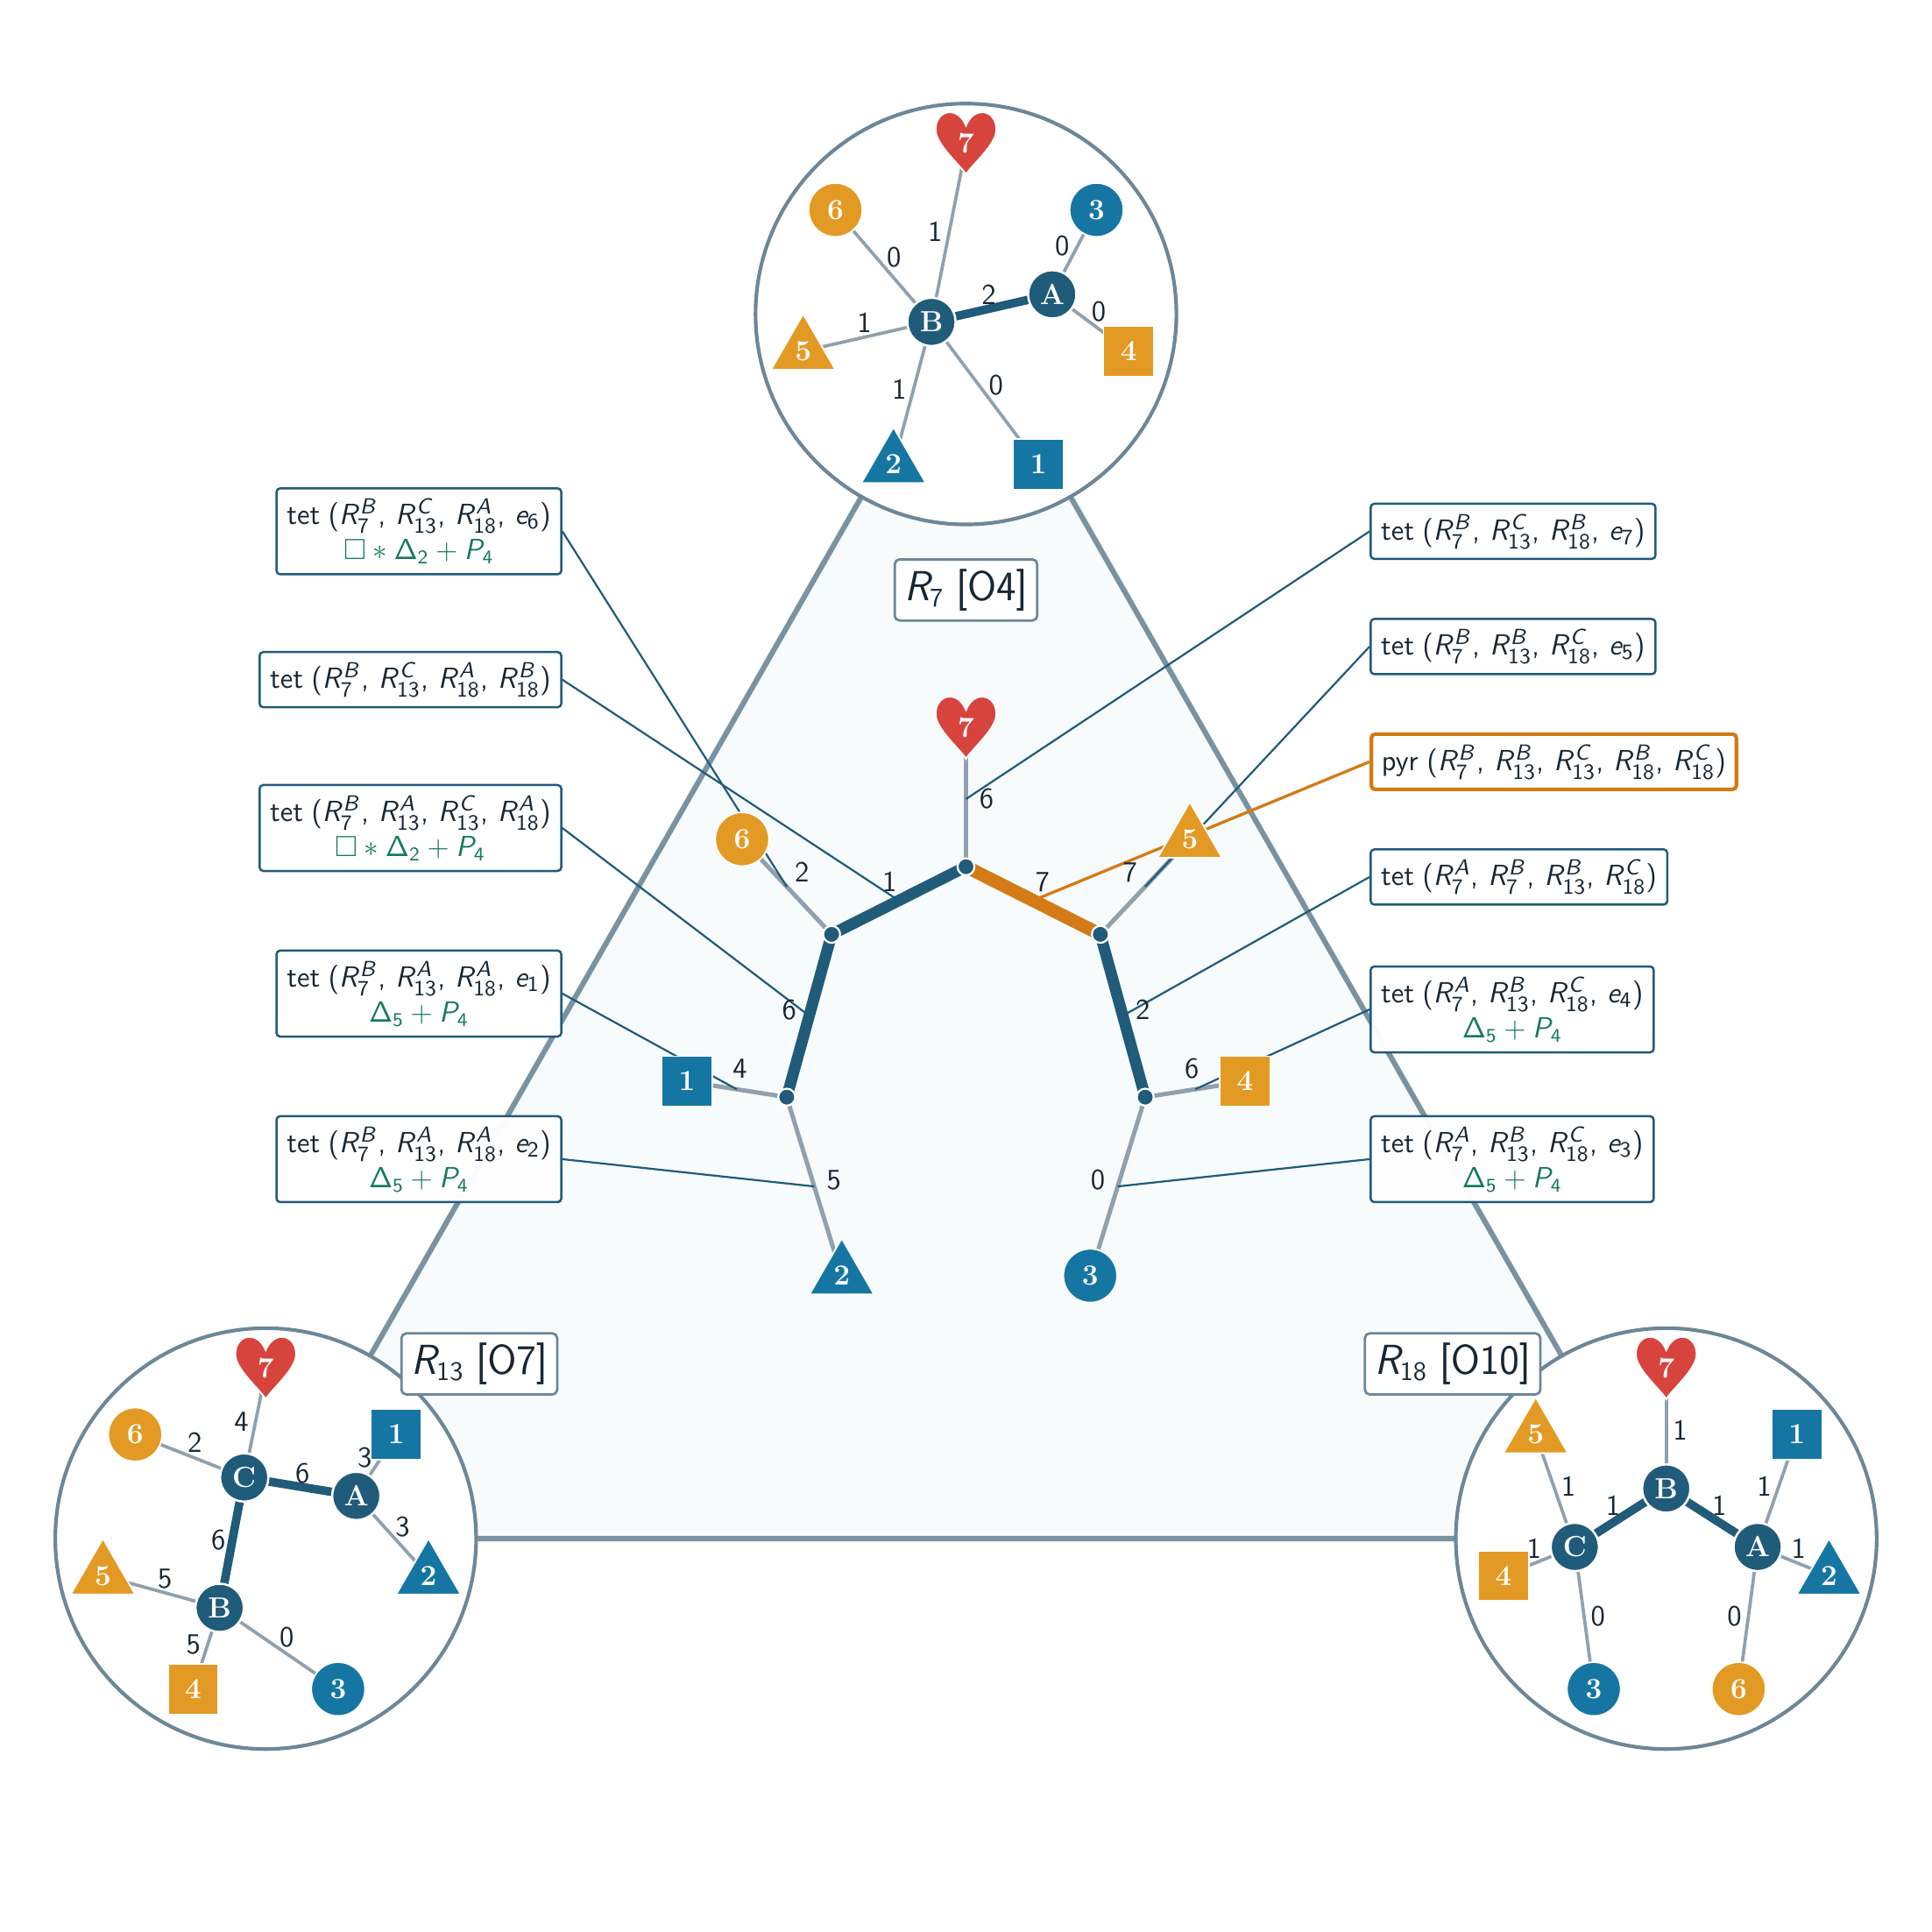
\begin{tikzpicture}[x=1cm,y=1cm]
\path[use as bounding box] (-13.65,-13.65) rectangle (13.65,13.65);
\path[support cell] (0.00000,9.45000)--(-10.15000,-8.30000)--(10.15000,-8.30000)--cycle;
\path[vertex disc] (0.00000,9.45000) circle[radius=3.05000cm];
\path[vertex disc] (-10.15000,-8.30000) circle[radius=3.05000cm];
\path[vertex disc] (10.15000,-8.30000) circle[radius=3.05000cm];
\coordinate (corner-1-v1) at (1.05000,7.26966);
\coordinate (corner-1-v2) at (-1.05000,7.26966);
\coordinate (corner-1-v3) at (1.89203,10.95885);
\coordinate (corner-1-v4) at (2.35933,8.91150);
\coordinate (corner-1-v5) at (-2.35933,8.91150);
\coordinate (corner-1-v6) at (-1.89203,10.95885);
\coordinate (corner-1-v7) at (0.00000,11.87000);
\coordinate (corner-1-v8) at (1.25040,9.73540);
\coordinate (corner-1-v9) at (-0.50016,9.33584);
\draw[internal edge] (corner-1-v8)--node[mini length,pos=0.5] {\(2\)}(corner-1-v9);
\draw[pendant edge] (corner-1-v1)--node[mini length,pos=0.5] {\(0\)}(corner-1-v9);
\draw[pendant edge] (corner-1-v2)--node[mini length,pos=0.5] {\(1\)}(corner-1-v9);
\draw[pendant edge] (corner-1-v3)--node[mini length,pos=0.5] {\(0\)}(corner-1-v8);
\draw[pendant edge] (corner-1-v4)--node[mini length,pos=0.5] {\(0\)}(corner-1-v8);
\draw[pendant edge] (corner-1-v5)--node[mini length,pos=0.5] {\(1\)}(corner-1-v9);
\draw[pendant edge] (corner-1-v6)--node[mini length,pos=0.5] {\(0\)}(corner-1-v9);
\draw[pendant edge] (corner-1-v7)--node[mini length,pos=0.5] {\(1\)}(corner-1-v9);
\node[lettered vertex] at (corner-1-v8) {A};
\node[lettered vertex] at (corner-1-v9) {B};
\taxonone{corner-1-v1}
\taxontwo{corner-1-v2}
\taxonthree{corner-1-v3}
\taxonfour{corner-1-v4}
\taxonfive{corner-1-v5}
\taxonsix{corner-1-v6}
\taxonseven{corner-1-v7}
\node[ray title] at (0.00000,5.45000) {\(R_{7}\;[\mathrm{O}4]\)};
\coordinate (corner-2-v1) at (-8.25797,-6.79115);
\coordinate (corner-2-v2) at (-7.79067,-8.83850);
\coordinate (corner-2-v3) at (-9.10000,-10.48034);
\coordinate (corner-2-v4) at (-11.20000,-10.48034);
\coordinate (corner-2-v5) at (-12.50933,-8.83850);
\coordinate (corner-2-v6) at (-12.04203,-6.79115);
\coordinate (corner-2-v7) at (-10.15000,-5.88000);
\coordinate (corner-2-v8) at (-8.83676,-7.68119);
\coordinate (corner-2-v9) at (-10.81774,-9.30327);
\coordinate (corner-2-v10) at (-10.46163,-7.41390);
\draw[internal edge] (corner-2-v8)--node[mini length,pos=0.5] {\(6\)}(corner-2-v10);
\draw[internal edge] (corner-2-v9)--node[mini length,pos=0.5] {\(6\)}(corner-2-v10);
\draw[pendant edge] (corner-2-v1)--node[mini length,pos=0.5] {\(3\)}(corner-2-v8);
\draw[pendant edge] (corner-2-v2)--node[mini length,pos=0.5] {\(3\)}(corner-2-v8);
\draw[pendant edge] (corner-2-v3)--node[mini length,pos=0.5] {\(0\)}(corner-2-v9);
\draw[pendant edge] (corner-2-v4)--node[mini length,pos=0.5] {\(5\)}(corner-2-v9);
\draw[pendant edge] (corner-2-v5)--node[mini length,pos=0.5] {\(5\)}(corner-2-v9);
\draw[pendant edge] (corner-2-v6)--node[mini length,pos=0.5] {\(2\)}(corner-2-v10);
\draw[pendant edge] (corner-2-v7)--node[mini length,pos=0.5] {\(4\)}(corner-2-v10);
\node[lettered vertex] at (corner-2-v8) {A};
\node[lettered vertex] at (corner-2-v9) {B};
\node[lettered vertex] at (corner-2-v10) {C};
\taxonone{corner-2-v1}
\taxontwo{corner-2-v2}
\taxonthree{corner-2-v3}
\taxonfour{corner-2-v4}
\taxonfive{corner-2-v5}
\taxonsix{corner-2-v6}
\taxonseven{corner-2-v7}
\node[ray title] at (-7.05349,-5.76788) {\(R_{13}\;[\mathrm{O}7]\)};
\coordinate (corner-3-v1) at (12.04203,-6.79115);
\coordinate (corner-3-v2) at (12.50933,-8.83850);
\coordinate (corner-3-v3) at (9.10000,-10.48034);
\coordinate (corner-3-v4) at (7.79067,-8.83850);
\coordinate (corner-3-v5) at (8.25797,-6.79115);
\coordinate (corner-3-v6) at (11.20000,-10.48034);
\coordinate (corner-3-v7) at (10.15000,-5.88000);
\coordinate (corner-3-v8) at (11.47534,-8.42100);
\coordinate (corner-3-v9) at (10.15000,-7.57400);
\coordinate (corner-3-v10) at (8.82466,-8.42100);
\draw[internal edge] (corner-3-v8)--node[mini length,pos=0.5] {\(1\)}(corner-3-v9);
\draw[internal edge] (corner-3-v9)--node[mini length,pos=0.5] {\(1\)}(corner-3-v10);
\draw[pendant edge] (corner-3-v1)--node[mini length,pos=0.5] {\(1\)}(corner-3-v8);
\draw[pendant edge] (corner-3-v2)--node[mini length,pos=0.5] {\(1\)}(corner-3-v8);
\draw[pendant edge] (corner-3-v3)--node[mini length,pos=0.5] {\(0\)}(corner-3-v10);
\draw[pendant edge] (corner-3-v4)--node[mini length,pos=0.5] {\(1\)}(corner-3-v10);
\draw[pendant edge] (corner-3-v5)--node[mini length,pos=0.5] {\(1\)}(corner-3-v10);
\draw[pendant edge] (corner-3-v6)--node[mini length,pos=0.5] {\(0\)}(corner-3-v8);
\draw[pendant edge] (corner-3-v7)--node[mini length,pos=0.5] {\(1\)}(corner-3-v9);
\node[lettered vertex] at (corner-3-v8) {A};
\node[lettered vertex] at (corner-3-v9) {B};
\node[lettered vertex] at (corner-3-v10) {C};
\taxonone{corner-3-v1}
\taxontwo{corner-3-v2}
\taxonthree{corner-3-v3}
\taxonfour{corner-3-v4}
\taxonfive{corner-3-v5}
\taxonsix{corner-3-v6}
\taxonseven{corner-3-v7}
\node[ray title] at (7.05349,-5.76788) {\(R_{18}\;[\mathrm{O}10]\)};
\coordinate (central-v1) at (-4.04595,-1.67346);
\coordinate (central-v2) at (-1.80062,-4.48902);
\coordinate (central-v3) at (1.80062,-4.48902);
\coordinate (central-v4) at (4.04595,-1.67346);
\coordinate (central-v5) at (3.24460,1.83748);
\coordinate (central-v6) at (-3.24460,1.83748);
\coordinate (central-v7) at (0.00000,3.40000);
\coordinate (central-v8) at (-2.59804,-1.90139);
\coordinate (central-v9) at (2.59804,-1.90139);
\coordinate (central-v10) at (1.94755,0.45833);
\coordinate (central-v11) at (-1.94755,0.45833);
\coordinate (central-v12) at (0.00000,1.43889);
\draw[central internal edge] (central-v8)--(central-v11);
\draw[central internal edge] (central-v9)--(central-v10);
\draw[central pyramid edge] (central-v10)--(central-v12);
\draw[central internal edge] (central-v11)--(central-v12);
\draw[central pendant edge] (central-v1)--(central-v8);
\draw[central pendant edge] (central-v2)--(central-v8);
\draw[central pendant edge] (central-v3)--(central-v9);
\draw[central pendant edge] (central-v4)--(central-v9);
\draw[central pendant edge] (central-v5)--(central-v10);
\draw[central pendant edge] (central-v6)--(central-v11);
\draw[central pendant edge] (central-v7)--(central-v12);
\draw[edge leader] (-5.85000,6.30000)--(-2.59607,1.14791);
\draw[edge leader] (-5.85000,4.15000)--(-0.97377,0.94861);
\draw[edge leader] (-5.85000,2.00000)--(-2.27279,-0.72153);
\draw[edge leader] (-5.85000,-0.40000)--(-3.32199,-1.78742);
\draw[edge leader] (-5.85000,-2.80000)--(-2.19933,-3.19520);
\draw[edge leader] (5.85000,6.30000)--(0.00000,2.41944);
\draw[edge leader] (5.85000,4.63000)--(2.59607,1.14791);
\draw[pyramid leader] (5.85000,2.96000)--(0.97377,0.94861);
\draw[edge leader] (5.85000,1.29000)--(2.27279,-0.72153);
\draw[edge leader] (5.85000,-0.63000)--(3.32199,-1.78742);
\draw[edge leader] (5.85000,-2.80000)--(2.19933,-3.19520);
\node[internal vertex] at (central-v8) {};
\node[internal vertex] at (central-v9) {};
\node[internal vertex] at (central-v10) {};
\node[internal vertex] at (central-v11) {};
\node[internal vertex] at (central-v12) {};
\taxonone{central-v1}
\taxontwo{central-v2}
\taxonthree{central-v3}
\taxonfour{central-v4}
\taxonfive{central-v5}
\taxonsix{central-v6}
\taxonseven{central-v7}
\path (central-v8)--node[central length,pos=.50] {\(6\)}(central-v11);
\path (central-v9)--node[central length,pos=.50] {\(2\)}(central-v10);
\path (central-v10)--node[central length,pos=.50] {\(7\)}(central-v12);
\path (central-v11)--node[central length,pos=.50] {\(1\)}(central-v12);
\path (central-v1)--node[central length,pos=.50] {\(4\)}(central-v8);
\path (central-v2)--node[central length,pos=.50] {\(5\)}(central-v8);
\path (central-v3)--node[central length,pos=.50] {\(0\)}(central-v9);
\path (central-v4)--node[central length,pos=.50] {\(6\)}(central-v9);
\path (central-v5)--node[central length,pos=.50] {\(7\)}(central-v10);
\path (central-v6)--node[central length,pos=.50] {\(2\)}(central-v11);
\path (central-v7)--node[central length,pos=.50] {\(6\)}(central-v12);
\node[edge callout,anchor=east] (callout-1) at (-5.85000,6.30000) {\(\mathrm{tet}\;(R_{7}^{B},\,R_{13}^{C},\,R_{18}^{A},\,e_{6})\)\\{\fontsize{12}{14}\selectfont\color{toricgreen}\(\square\ast\Delta_{2}+P_{4}\)}};
\node[edge callout,anchor=east] (callout-2) at (-5.85000,4.15000) {\(\mathrm{tet}\;(R_{7}^{B},\,R_{13}^{C},\,R_{18}^{A},\,R_{18}^{B})\)};
\node[edge callout,anchor=east] (callout-3) at (-5.85000,2.00000) {\(\mathrm{tet}\;(R_{7}^{B},\,R_{13}^{A},\,R_{13}^{C},\,R_{18}^{A})\)\\{\fontsize{12}{14}\selectfont\color{toricgreen}\(\square\ast\Delta_{2}+P_{4}\)}};
\node[edge callout,anchor=east] (callout-4) at (-5.85000,-0.40000) {\(\mathrm{tet}\;(R_{7}^{B},\,R_{13}^{A},\,R_{18}^{A},\,e_{1})\)\\{\fontsize{12}{14}\selectfont\color{toricgreen}\(\Delta_{5}+P_{4}\)}};
\node[edge callout,anchor=east] (callout-5) at (-5.85000,-2.80000) {\(\mathrm{tet}\;(R_{7}^{B},\,R_{13}^{A},\,R_{18}^{A},\,e_{2})\)\\{\fontsize{12}{14}\selectfont\color{toricgreen}\(\Delta_{5}+P_{4}\)}};
\node[edge callout,anchor=west] (callout-6) at (5.85000,6.30000) {\(\mathrm{tet}\;(R_{7}^{B},\,R_{13}^{C},\,R_{18}^{B},\,e_{7})\)};
\node[edge callout,anchor=west] (callout-7) at (5.85000,4.63000) {\(\mathrm{tet}\;(R_{7}^{B},\,R_{13}^{B},\,R_{18}^{C},\,e_{5})\)};
\node[pyramid callout,anchor=west] (callout-8) at (5.85000,2.96000) {\(\mathrm{pyr}\;(R_{7}^{B},\,R_{13}^{B},\,R_{13}^{C},\,R_{18}^{B},\,R_{18}^{C})\)};
\node[edge callout,anchor=west] (callout-9) at (5.85000,1.29000) {\(\mathrm{tet}\;(R_{7}^{A},\,R_{7}^{B},\,R_{13}^{B},\,R_{18}^{C})\)};
\node[edge callout,anchor=west] (callout-10) at (5.85000,-0.63000) {\(\mathrm{tet}\;(R_{7}^{A},\,R_{13}^{B},\,R_{18}^{C},\,e_{4})\)\\{\fontsize{12}{14}\selectfont\color{toricgreen}\(\Delta_{5}+P_{4}\)}};
\node[edge callout,anchor=west] (callout-11) at (5.85000,-2.80000) {\(\mathrm{tet}\;(R_{7}^{A},\,R_{13}^{B},\,R_{18}^{C},\,e_{3})\)\\{\fontsize{12}{14}\selectfont\color{toricgreen}\(\Delta_{5}+P_{4}\)}};
\end{tikzpicture}\end{center}\vspace{-1mm}
\begin{atlasbox}\begin{atlaspanel}
\textcolor{toricgreen}{\bfseries PRIME TORIC}\quad \(P_{4}\):\enspace \(\square\ast\Delta_{2}\)\quad \(f=(7,19,26,19,7)\)\quad 14 lattice points
\end{atlaspanel}\end{atlasbox}
\clearpage
\begin{atlaspanel}[top=1mm,bottom=2mm]
\AtlasSupportOrbitSplit{%
\vspace*{-3mm}\mbox{{\LARGE\bfseries Triangle orbit 5}\hspace{3mm}\raisebox{.8mm}[0pt][0pt]{{\fontsize{16}{18}\selectfont\color{muted}size 6}}}%
}{%
\vspace*{-3mm}{\fontsize{13}{16}\selectfont{\color{muted}\(\mathbb{Q}\) and \(\mathbb{F}_2\)}\quad{\color{muted}\(\underline{\{2,\,13,\,14\}}\), \(\{14,\,17,\,28\}\), \(\{20,\,22,\,32\}\), \(\{19,\,21,\,31\}\), \(\{22,\,25,\,44\}\), \(\{21,\,26,\,45\}\)}\rule[-3mm]{0pt}{3mm}}%
}%
\end{atlaspanel}\vspace{2mm}
\begin{center}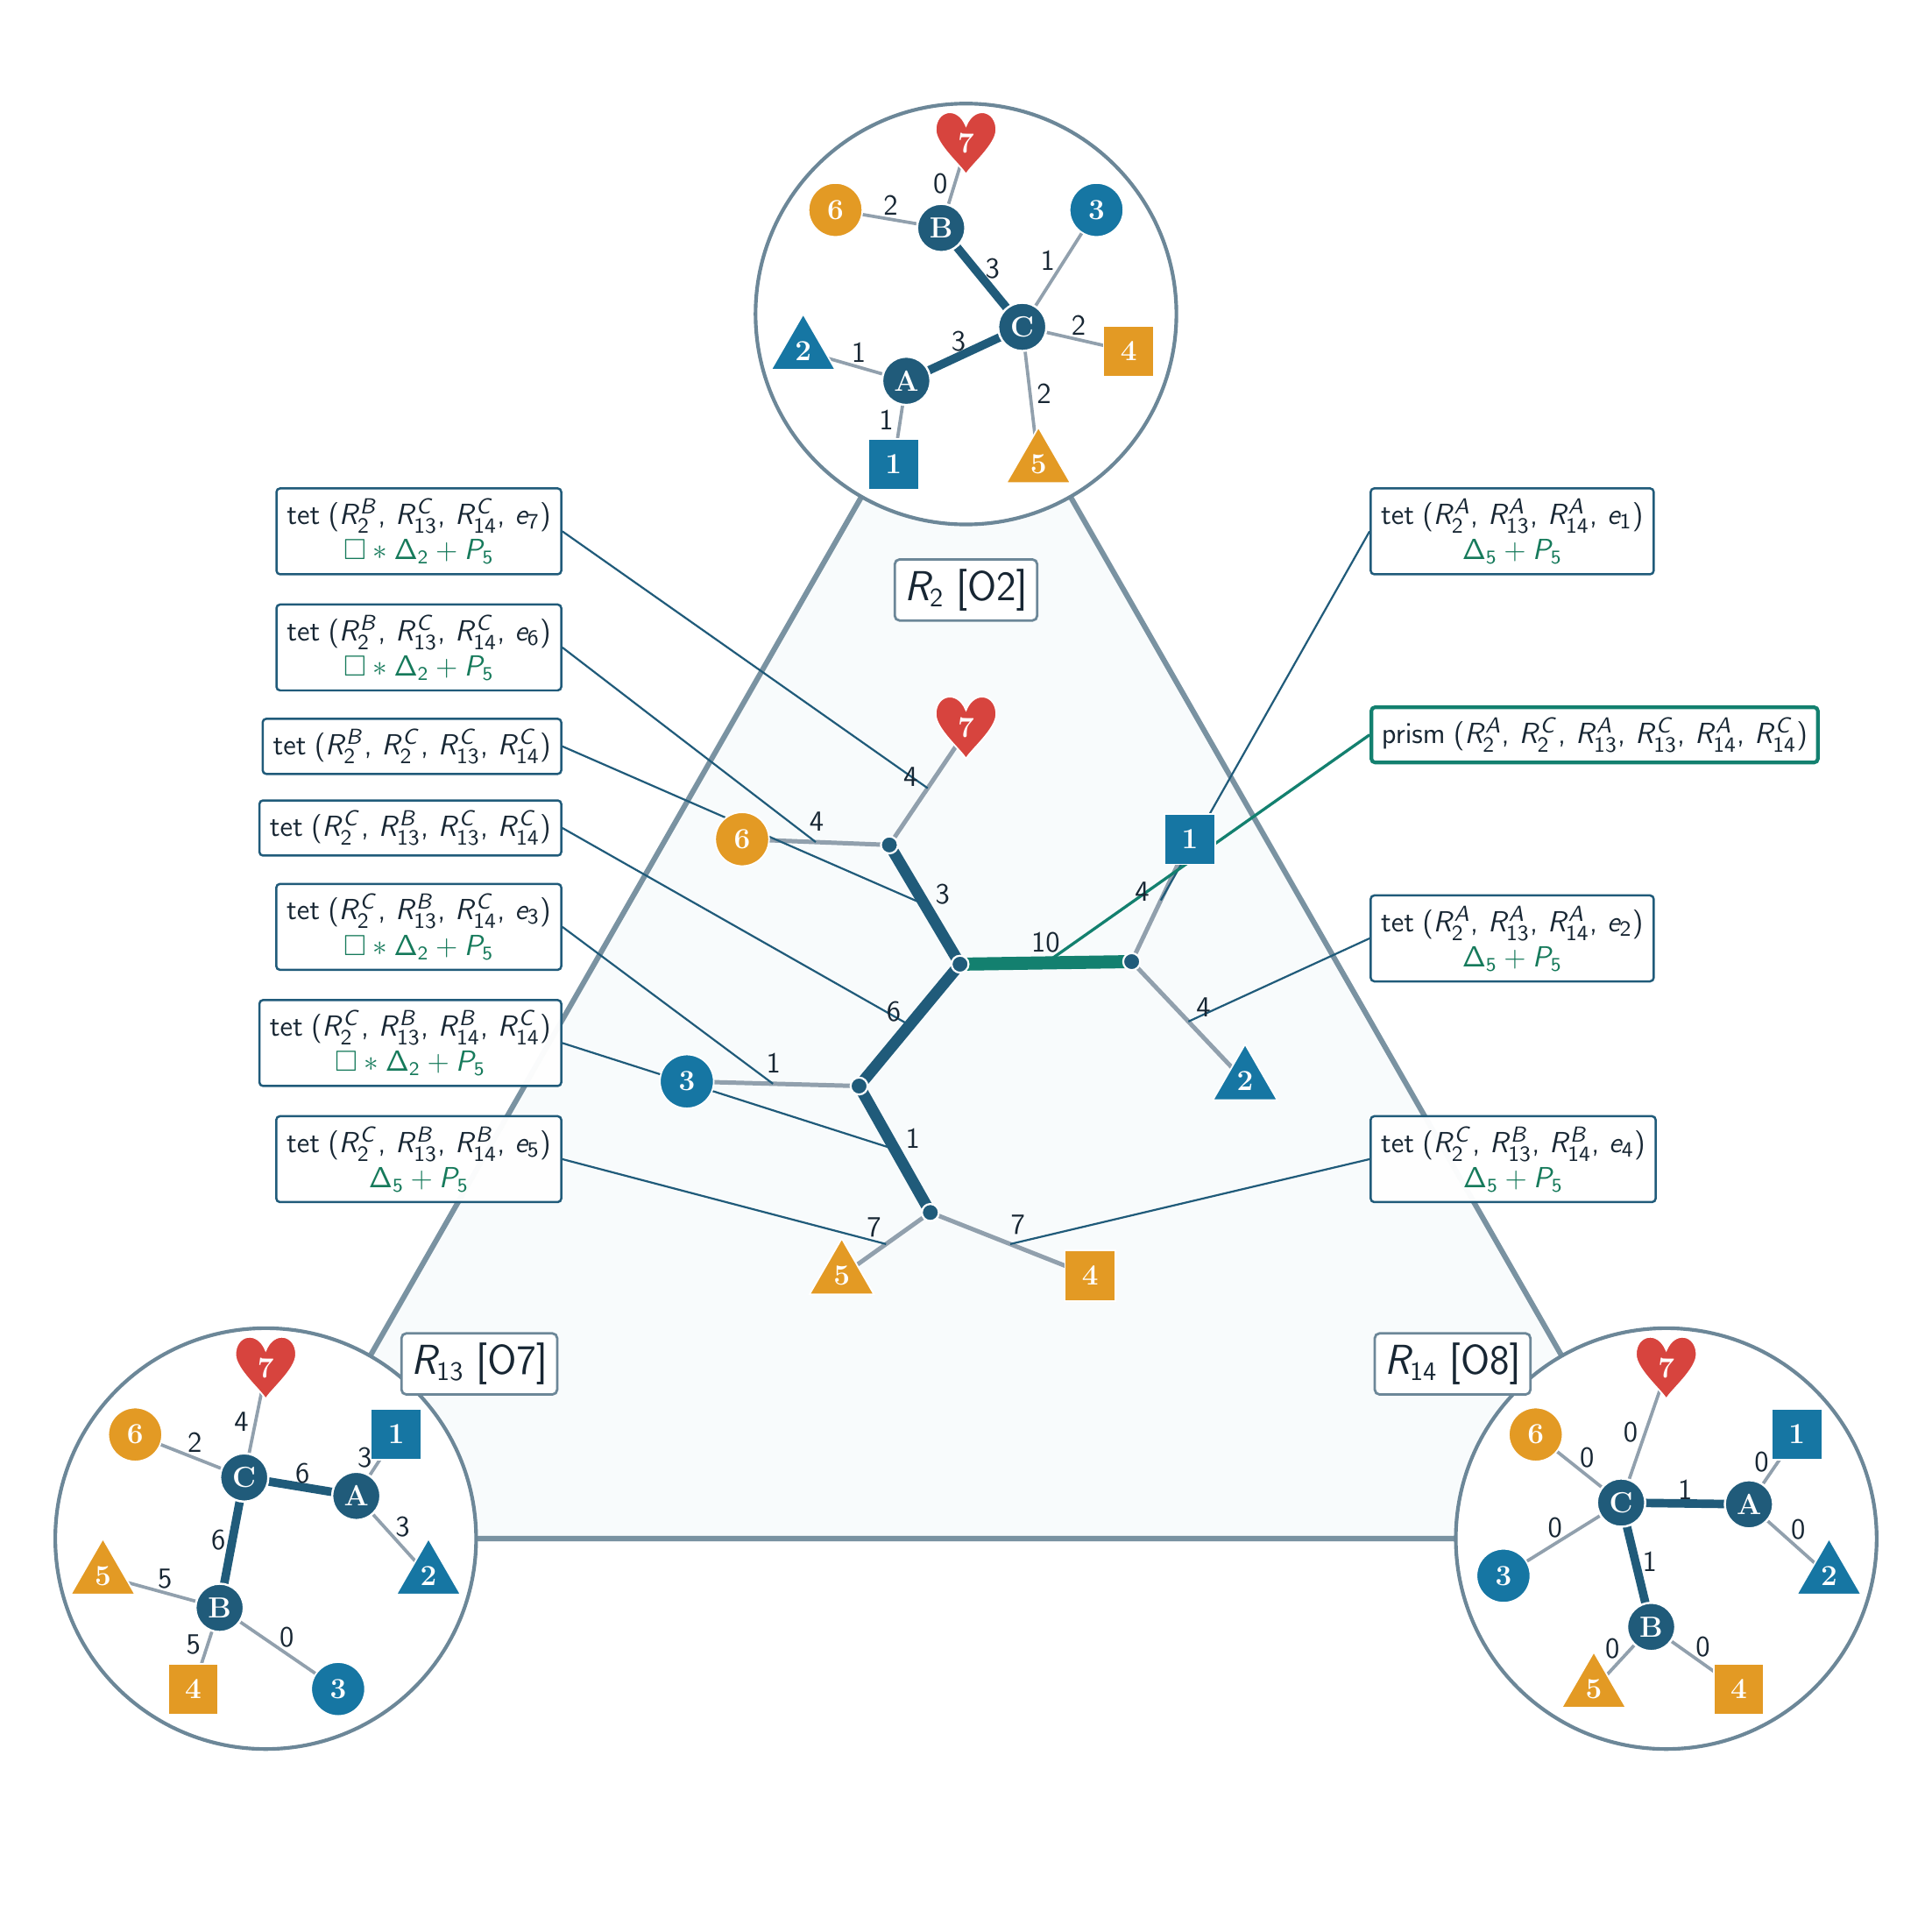
\begin{tikzpicture}[x=1cm,y=1cm]
\path[use as bounding box] (-13.65,-13.65) rectangle (13.65,13.65);
\path[support cell] (0.00000,9.45000)--(-10.15000,-8.30000)--(10.15000,-8.30000)--cycle;
\path[vertex disc] (0.00000,9.45000) circle[radius=3.05000cm];
\path[vertex disc] (-10.15000,-8.30000) circle[radius=3.05000cm];
\path[vertex disc] (10.15000,-8.30000) circle[radius=3.05000cm];
\coordinate (corner-1-v1) at (-1.05000,7.26966);
\coordinate (corner-1-v2) at (-2.35933,8.91150);
\coordinate (corner-1-v3) at (1.89203,10.95885);
\coordinate (corner-1-v4) at (2.35933,8.91150);
\coordinate (corner-1-v5) at (1.05000,7.26966);
\coordinate (corner-1-v6) at (-1.89203,10.95885);
\coordinate (corner-1-v7) at (0.00000,11.87000);
\coordinate (corner-1-v8) at (-0.86458,8.48167);
\coordinate (corner-1-v9) at (-0.35881,10.69756);
\coordinate (corner-1-v10) at (0.81559,9.26385);
\draw[internal edge] (corner-1-v8)--node[mini length,pos=0.5] {\(3\)}(corner-1-v10);
\draw[internal edge] (corner-1-v9)--node[mini length,pos=0.5] {\(3\)}(corner-1-v10);
\draw[pendant edge] (corner-1-v1)--node[mini length,pos=0.5] {\(1\)}(corner-1-v8);
\draw[pendant edge] (corner-1-v2)--node[mini length,pos=0.5] {\(1\)}(corner-1-v8);
\draw[pendant edge] (corner-1-v3)--node[mini length,pos=0.5] {\(1\)}(corner-1-v10);
\draw[pendant edge] (corner-1-v4)--node[mini length,pos=0.5] {\(2\)}(corner-1-v10);
\draw[pendant edge] (corner-1-v5)--node[mini length,pos=0.5] {\(2\)}(corner-1-v10);
\draw[pendant edge] (corner-1-v6)--node[mini length,pos=0.5] {\(2\)}(corner-1-v9);
\draw[pendant edge] (corner-1-v7)--node[mini length,pos=0.5] {\(0\)}(corner-1-v9);
\node[lettered vertex] at (corner-1-v8) {A};
\node[lettered vertex] at (corner-1-v9) {B};
\node[lettered vertex] at (corner-1-v10) {C};
\taxonone{corner-1-v1}
\taxontwo{corner-1-v2}
\taxonthree{corner-1-v3}
\taxonfour{corner-1-v4}
\taxonfive{corner-1-v5}
\taxonsix{corner-1-v6}
\taxonseven{corner-1-v7}
\node[ray title] at (0.00000,5.45000) {\(R_{2}\;[\mathrm{O}2]\)};
\coordinate (corner-2-v1) at (-8.25797,-6.79115);
\coordinate (corner-2-v2) at (-7.79067,-8.83850);
\coordinate (corner-2-v3) at (-9.10000,-10.48034);
\coordinate (corner-2-v4) at (-11.20000,-10.48034);
\coordinate (corner-2-v5) at (-12.50933,-8.83850);
\coordinate (corner-2-v6) at (-12.04203,-6.79115);
\coordinate (corner-2-v7) at (-10.15000,-5.88000);
\coordinate (corner-2-v8) at (-8.83676,-7.68119);
\coordinate (corner-2-v9) at (-10.81774,-9.30327);
\coordinate (corner-2-v10) at (-10.46163,-7.41390);
\draw[internal edge] (corner-2-v8)--node[mini length,pos=0.5] {\(6\)}(corner-2-v10);
\draw[internal edge] (corner-2-v9)--node[mini length,pos=0.5] {\(6\)}(corner-2-v10);
\draw[pendant edge] (corner-2-v1)--node[mini length,pos=0.5] {\(3\)}(corner-2-v8);
\draw[pendant edge] (corner-2-v2)--node[mini length,pos=0.5] {\(3\)}(corner-2-v8);
\draw[pendant edge] (corner-2-v3)--node[mini length,pos=0.5] {\(0\)}(corner-2-v9);
\draw[pendant edge] (corner-2-v4)--node[mini length,pos=0.5] {\(5\)}(corner-2-v9);
\draw[pendant edge] (corner-2-v5)--node[mini length,pos=0.5] {\(5\)}(corner-2-v9);
\draw[pendant edge] (corner-2-v6)--node[mini length,pos=0.5] {\(2\)}(corner-2-v10);
\draw[pendant edge] (corner-2-v7)--node[mini length,pos=0.5] {\(4\)}(corner-2-v10);
\node[lettered vertex] at (corner-2-v8) {A};
\node[lettered vertex] at (corner-2-v9) {B};
\node[lettered vertex] at (corner-2-v10) {C};
\taxonone{corner-2-v1}
\taxontwo{corner-2-v2}
\taxonthree{corner-2-v3}
\taxonfour{corner-2-v4}
\taxonfive{corner-2-v5}
\taxonsix{corner-2-v6}
\taxonseven{corner-2-v7}
\node[ray title] at (-7.05349,-5.76788) {\(R_{13}\;[\mathrm{O}7]\)};
\coordinate (corner-3-v1) at (12.04203,-6.79115);
\coordinate (corner-3-v2) at (12.50933,-8.83850);
\coordinate (corner-3-v3) at (7.79067,-8.83850);
\coordinate (corner-3-v4) at (11.20000,-10.48034);
\coordinate (corner-3-v5) at (9.10000,-10.48034);
\coordinate (corner-3-v6) at (8.25797,-6.79115);
\coordinate (corner-3-v7) at (10.15000,-5.88000);
\coordinate (corner-3-v8) at (11.34910,-7.80269);
\coordinate (corner-3-v9) at (9.93198,-9.57970);
\coordinate (corner-3-v10) at (9.49594,-7.77841);
\draw[internal edge] (corner-3-v8)--node[mini length,pos=0.5] {\(1\)}(corner-3-v10);
\draw[internal edge] (corner-3-v9)--node[mini length,pos=0.5] {\(1\)}(corner-3-v10);
\draw[pendant edge] (corner-3-v1)--node[mini length,pos=0.5] {\(0\)}(corner-3-v8);
\draw[pendant edge] (corner-3-v2)--node[mini length,pos=0.5] {\(0\)}(corner-3-v8);
\draw[pendant edge] (corner-3-v3)--node[mini length,pos=0.5] {\(0\)}(corner-3-v10);
\draw[pendant edge] (corner-3-v4)--node[mini length,pos=0.5] {\(0\)}(corner-3-v9);
\draw[pendant edge] (corner-3-v5)--node[mini length,pos=0.5] {\(0\)}(corner-3-v9);
\draw[pendant edge] (corner-3-v6)--node[mini length,pos=0.5] {\(0\)}(corner-3-v10);
\draw[pendant edge] (corner-3-v7)--node[mini length,pos=0.5] {\(0\)}(corner-3-v10);
\node[lettered vertex] at (corner-3-v8) {A};
\node[lettered vertex] at (corner-3-v9) {B};
\node[lettered vertex] at (corner-3-v10) {C};
\taxonone{corner-3-v1}
\taxontwo{corner-3-v2}
\taxonthree{corner-3-v3}
\taxonfour{corner-3-v4}
\taxonfive{corner-3-v5}
\taxonsix{corner-3-v6}
\taxonseven{corner-3-v7}
\node[ray title] at (7.05349,-5.76788) {\(R_{14}\;[\mathrm{O}8]\)};
\coordinate (central-v1) at (3.24460,1.83748);
\coordinate (central-v2) at (4.04595,-1.67346);
\coordinate (central-v3) at (-4.04595,-1.67346);
\coordinate (central-v4) at (1.80062,-4.48902);
\coordinate (central-v5) at (-1.80062,-4.48902);
\coordinate (central-v6) at (-3.24460,1.83748);
\coordinate (central-v7) at (0.00000,3.40000);
\coordinate (central-v8) at (2.40149,0.06330);
\coordinate (central-v9) at (-1.11023,1.75446);
\coordinate (central-v10) at (-0.08608,0.02589);
\coordinate (central-v11) at (-1.54951,-1.74010);
\coordinate (central-v12) at (-0.51650,-3.57271);
\draw[central prism edge] (central-v8)--(central-v10);
\draw[central internal edge] (central-v9)--(central-v10);
\draw[central internal edge] (central-v10)--(central-v11);
\draw[central internal edge] (central-v11)--(central-v12);
\draw[central pendant edge] (central-v1)--(central-v8);
\draw[central pendant edge] (central-v2)--(central-v8);
\draw[central pendant edge] (central-v3)--(central-v11);
\draw[central pendant edge] (central-v4)--(central-v12);
\draw[central pendant edge] (central-v5)--(central-v12);
\draw[central pendant edge] (central-v6)--(central-v9);
\draw[central pendant edge] (central-v7)--(central-v9);
\draw[edge leader] (-5.85000,6.30000)--(-0.55511,2.57723);
\draw[edge leader] (-5.85000,4.61667)--(-2.17741,1.79597);
\draw[edge leader] (-5.85000,3.18333)--(-0.59816,0.89017);
\draw[edge leader] (-5.85000,2.00000)--(-0.81780,-0.85710);
\draw[edge leader] (-5.85000,0.56667)--(-2.79773,-1.70678);
\draw[edge leader] (-5.85000,-1.11667)--(-1.03301,-2.65640);
\draw[edge leader] (-5.85000,-2.80000)--(-1.15856,-4.03087);
\draw[edge leader] (5.85000,6.30000)--(2.82304,0.95039);
\draw[prism leader] (5.85000,3.35000)--(1.15770,0.04460);
\draw[edge leader] (5.85000,0.40000)--(3.22372,-0.80508);
\draw[edge leader] (5.85000,-2.80000)--(0.64206,-4.03087);
\node[internal vertex] at (central-v8) {};
\node[internal vertex] at (central-v9) {};
\node[internal vertex] at (central-v10) {};
\node[internal vertex] at (central-v11) {};
\node[internal vertex] at (central-v12) {};
\taxonone{central-v1}
\taxontwo{central-v2}
\taxonthree{central-v3}
\taxonfour{central-v4}
\taxonfive{central-v5}
\taxonsix{central-v6}
\taxonseven{central-v7}
\path (central-v8)--node[central length,pos=.50] {\(10\)}(central-v10);
\path (central-v9)--node[central length,pos=.50] {\(3\)}(central-v10);
\path (central-v10)--node[central length,pos=.50] {\(6\)}(central-v11);
\path (central-v11)--node[central length,pos=.50] {\(1\)}(central-v12);
\path (central-v1)--node[central length,pos=.50] {\(4\)}(central-v8);
\path (central-v2)--node[central length,pos=.50] {\(4\)}(central-v8);
\path (central-v3)--node[central length,pos=.50] {\(1\)}(central-v11);
\path (central-v4)--node[central length,pos=.50] {\(7\)}(central-v12);
\path (central-v5)--node[central length,pos=.50] {\(7\)}(central-v12);
\path (central-v6)--node[central length,pos=.50] {\(4\)}(central-v9);
\path (central-v7)--node[central length,pos=.50] {\(4\)}(central-v9);
\node[edge callout,anchor=east] (callout-1) at (-5.85000,6.30000) {\(\mathrm{tet}\;(R_{2}^{B},\,R_{13}^{C},\,R_{14}^{C},\,e_{7})\)\\{\fontsize{12}{14}\selectfont\color{toricgreen}\(\square\ast\Delta_{2}+P_{5}\)}};
\node[edge callout,anchor=east] (callout-2) at (-5.85000,4.61667) {\(\mathrm{tet}\;(R_{2}^{B},\,R_{13}^{C},\,R_{14}^{C},\,e_{6})\)\\{\fontsize{12}{14}\selectfont\color{toricgreen}\(\square\ast\Delta_{2}+P_{5}\)}};
\node[edge callout,anchor=east] (callout-3) at (-5.85000,3.18333) {\(\mathrm{tet}\;(R_{2}^{B},\,R_{2}^{C},\,R_{13}^{C},\,R_{14}^{C})\)};
\node[edge callout,anchor=east] (callout-4) at (-5.85000,2.00000) {\(\mathrm{tet}\;(R_{2}^{C},\,R_{13}^{B},\,R_{13}^{C},\,R_{14}^{C})\)};
\node[edge callout,anchor=east] (callout-5) at (-5.85000,0.56667) {\(\mathrm{tet}\;(R_{2}^{C},\,R_{13}^{B},\,R_{14}^{C},\,e_{3})\)\\{\fontsize{12}{14}\selectfont\color{toricgreen}\(\square\ast\Delta_{2}+P_{5}\)}};
\node[edge callout,anchor=east] (callout-6) at (-5.85000,-1.11667) {\(\mathrm{tet}\;(R_{2}^{C},\,R_{13}^{B},\,R_{14}^{B},\,R_{14}^{C})\)\\{\fontsize{12}{14}\selectfont\color{toricgreen}\(\square\ast\Delta_{2}+P_{5}\)}};
\node[edge callout,anchor=east] (callout-7) at (-5.85000,-2.80000) {\(\mathrm{tet}\;(R_{2}^{C},\,R_{13}^{B},\,R_{14}^{B},\,e_{5})\)\\{\fontsize{12}{14}\selectfont\color{toricgreen}\(\Delta_{5}+P_{5}\)}};
\node[edge callout,anchor=west] (callout-8) at (5.85000,6.30000) {\(\mathrm{tet}\;(R_{2}^{A},\,R_{13}^{A},\,R_{14}^{A},\,e_{1})\)\\{\fontsize{12}{14}\selectfont\color{toricgreen}\(\Delta_{5}+P_{5}\)}};
\node[prism callout,anchor=west] (callout-9) at (5.85000,3.35000) {\(\mathrm{prism}\;(R_{2}^{A},\,R_{2}^{C},\,R_{13}^{A},\,R_{13}^{C},\,R_{14}^{A},\,R_{14}^{C})\)};
\node[edge callout,anchor=west] (callout-10) at (5.85000,0.40000) {\(\mathrm{tet}\;(R_{2}^{A},\,R_{13}^{A},\,R_{14}^{A},\,e_{2})\)\\{\fontsize{12}{14}\selectfont\color{toricgreen}\(\Delta_{5}+P_{5}\)}};
\node[edge callout,anchor=west] (callout-11) at (5.85000,-2.80000) {\(\mathrm{tet}\;(R_{2}^{C},\,R_{13}^{B},\,R_{14}^{B},\,e_{4})\)\\{\fontsize{12}{14}\selectfont\color{toricgreen}\(\Delta_{5}+P_{5}\)}};
\end{tikzpicture}\end{center}\vspace{-1mm}
\begin{atlasbox}\begin{atlaspanel}
\textcolor{toricgreen}{\bfseries PRIME TORIC}\quad \(P_{5}\):\enspace \(\mathrm{Wed}(\square\ast\Delta_{0};\,\Delta_1)\ast\Delta_{0}\)\quad \(f=(9,26,35,24,8)\)\quad 14 lattice points
\end{atlaspanel}\end{atlasbox}
\clearpage
\begin{atlaspanel}[top=1mm,bottom=2mm]
\AtlasSupportOrbitSplit{%
\vspace*{-3mm}\mbox{{\LARGE\bfseries Triangle orbit 6}\hspace{3mm}\raisebox{.8mm}[0pt][0pt]{{\fontsize{16}{18}\selectfont\color{muted}size 3}}}%
}{%
\vspace*{-3mm}{\fontsize{13}{16}\selectfont{\color{muted}\(\mathbb{Q}\) and \(\mathbb{F}_2\)}\quad{\color{muted}\(\underline{\{8,\,14,\,30\}}\), \(\{10,\,22,\,33\}\), \(\{9,\,21,\,34\}\)}\rule[-3mm]{0pt}{3mm}}%
}%
\end{atlaspanel}\vspace{2mm}
\begin{center}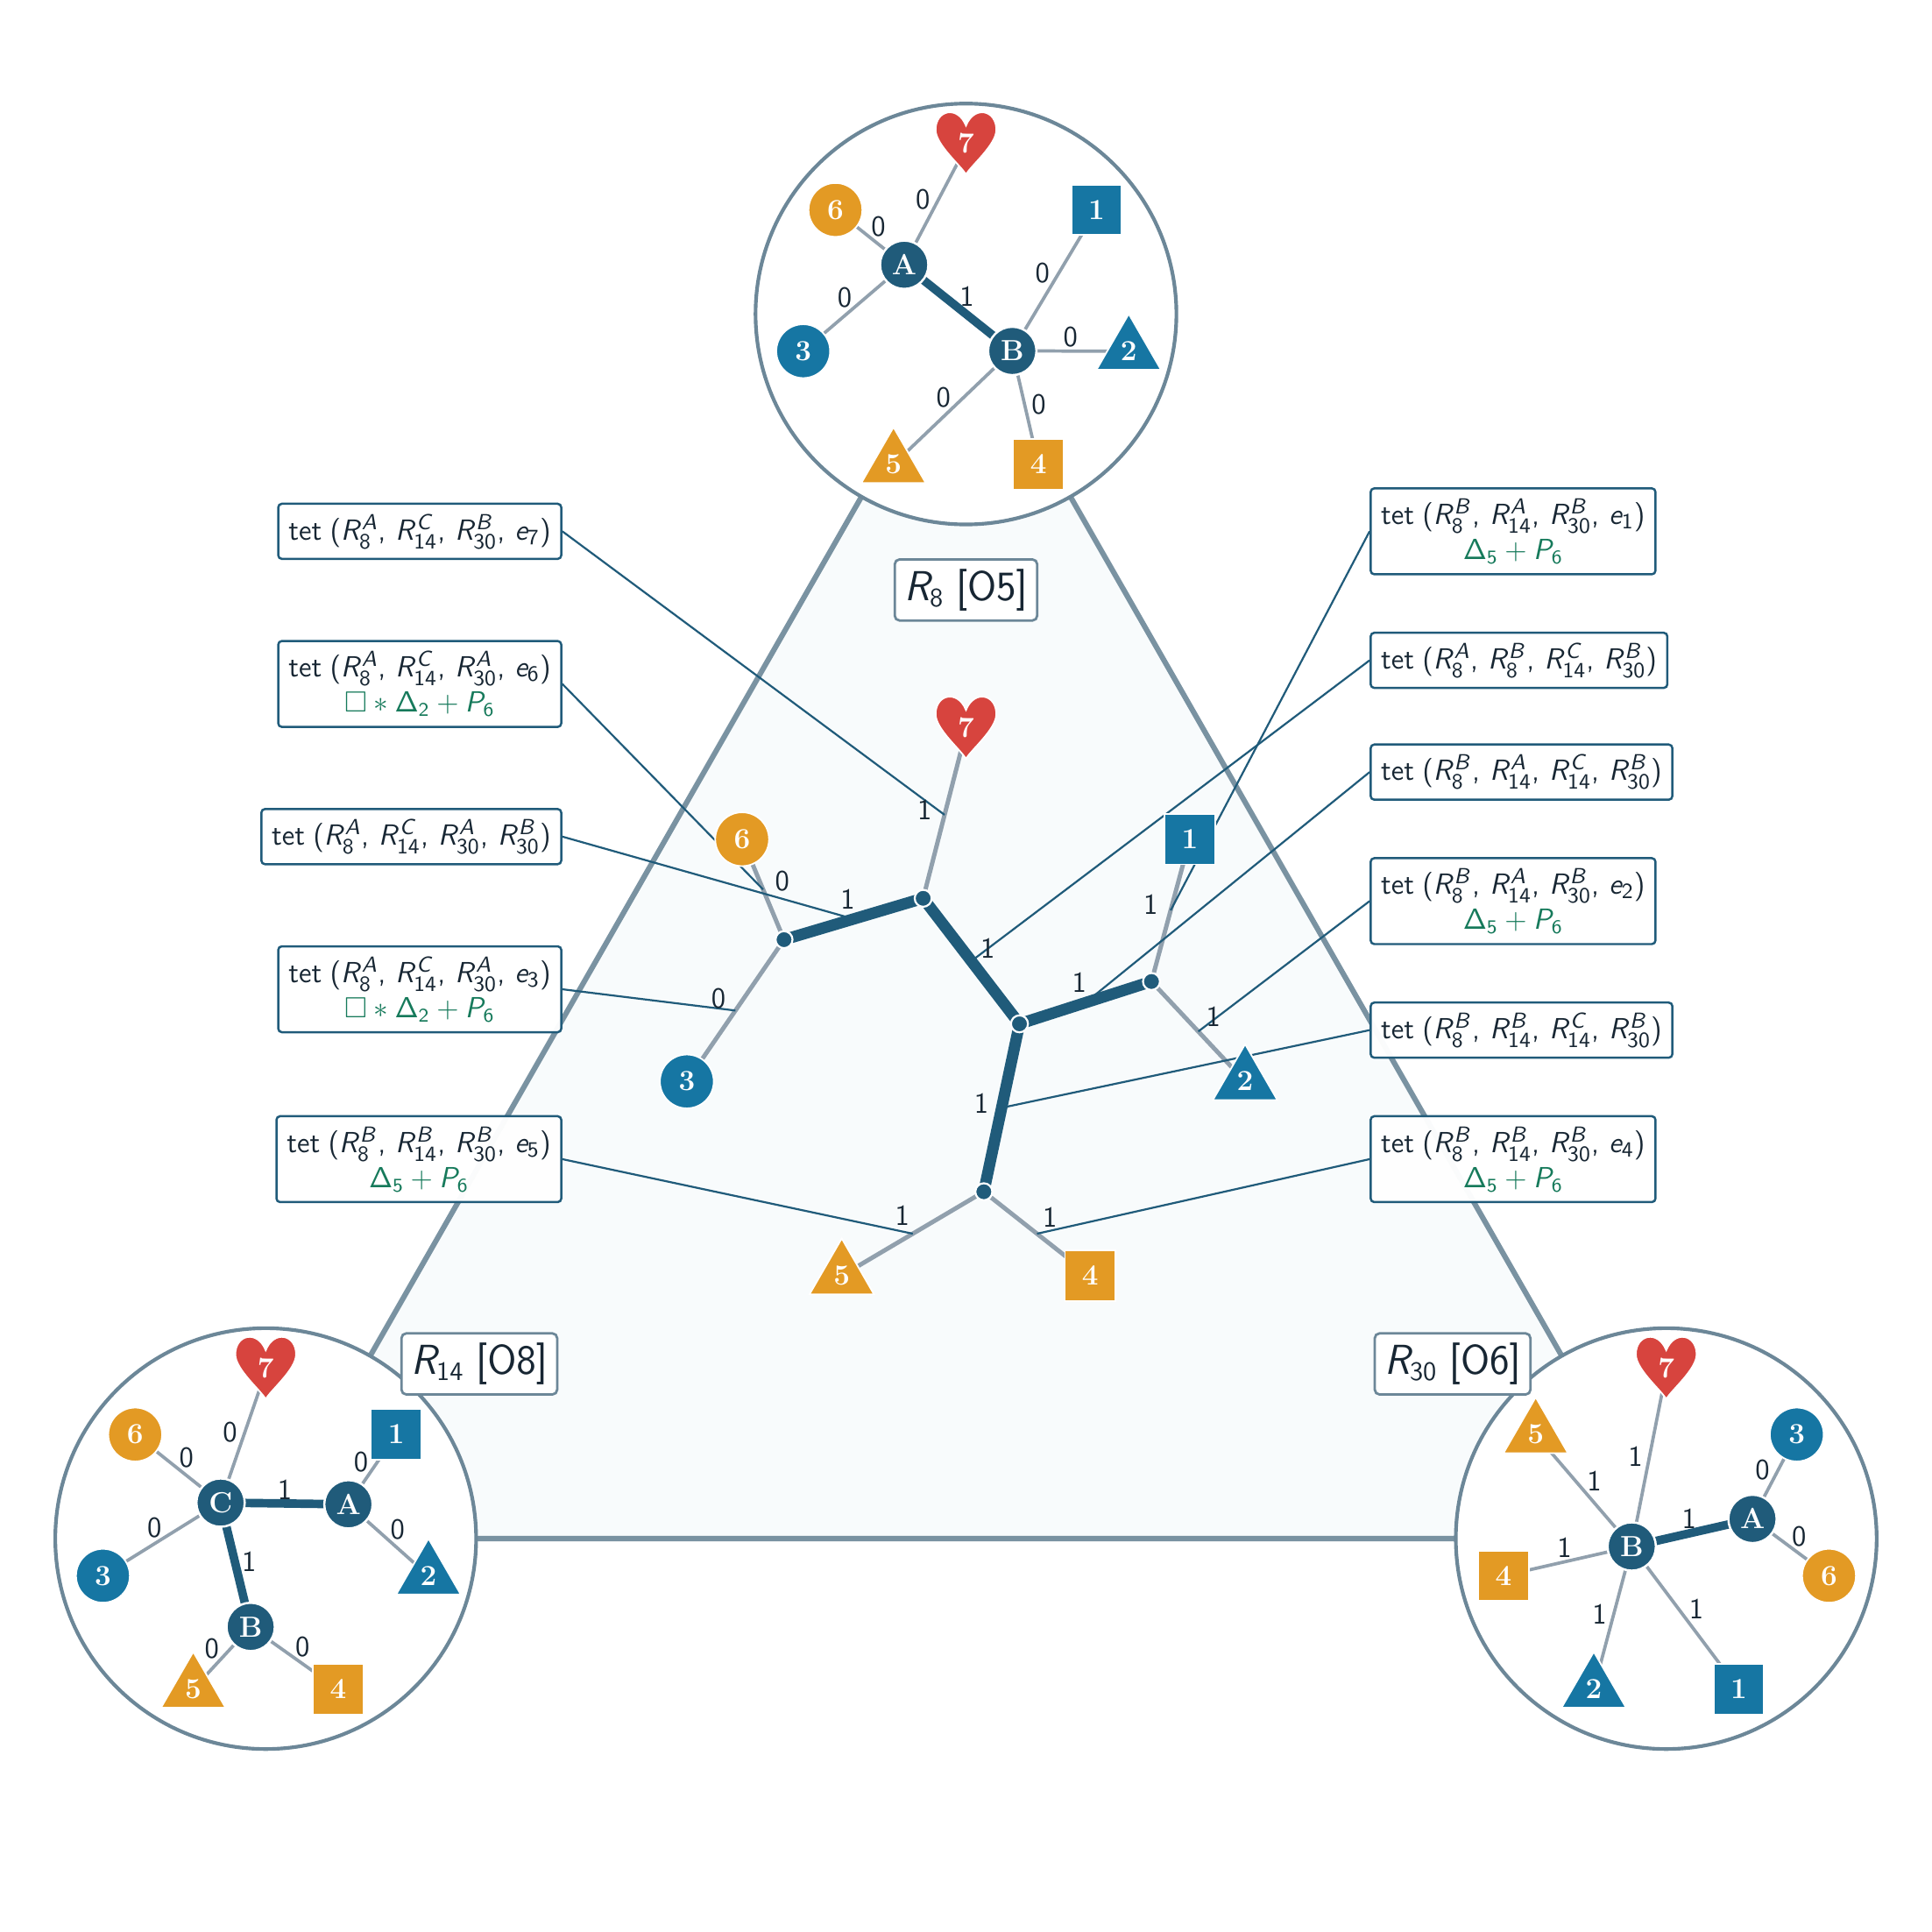
\begin{tikzpicture}[x=1cm,y=1cm]
\path[use as bounding box] (-13.65,-13.65) rectangle (13.65,13.65);
\path[support cell] (0.00000,9.45000)--(-10.15000,-8.30000)--(10.15000,-8.30000)--cycle;
\path[vertex disc] (0.00000,9.45000) circle[radius=3.05000cm];
\path[vertex disc] (-10.15000,-8.30000) circle[radius=3.05000cm];
\path[vertex disc] (10.15000,-8.30000) circle[radius=3.05000cm];
\coordinate (corner-1-v1) at (1.89203,10.95885);
\coordinate (corner-1-v2) at (2.35933,8.91150);
\coordinate (corner-1-v3) at (-2.35933,8.91150);
\coordinate (corner-1-v4) at (1.05000,7.26966);
\coordinate (corner-1-v5) at (-1.05000,7.26966);
\coordinate (corner-1-v6) at (-1.89203,10.95885);
\coordinate (corner-1-v7) at (0.00000,11.87000);
\coordinate (corner-1-v8) at (-0.89502,10.16376);
\coordinate (corner-1-v9) at (0.67127,8.91468);
\draw[internal edge] (corner-1-v8)--node[mini length,pos=0.5] {\(1\)}(corner-1-v9);
\draw[pendant edge] (corner-1-v1)--node[mini length,pos=0.5] {\(0\)}(corner-1-v9);
\draw[pendant edge] (corner-1-v2)--node[mini length,pos=0.5] {\(0\)}(corner-1-v9);
\draw[pendant edge] (corner-1-v3)--node[mini length,pos=0.5] {\(0\)}(corner-1-v8);
\draw[pendant edge] (corner-1-v4)--node[mini length,pos=0.5] {\(0\)}(corner-1-v9);
\draw[pendant edge] (corner-1-v5)--node[mini length,pos=0.5] {\(0\)}(corner-1-v9);
\draw[pendant edge] (corner-1-v6)--node[mini length,pos=0.5] {\(0\)}(corner-1-v8);
\draw[pendant edge] (corner-1-v7)--node[mini length,pos=0.5] {\(0\)}(corner-1-v8);
\node[lettered vertex] at (corner-1-v8) {A};
\node[lettered vertex] at (corner-1-v9) {B};
\taxonone{corner-1-v1}
\taxontwo{corner-1-v2}
\taxonthree{corner-1-v3}
\taxonfour{corner-1-v4}
\taxonfive{corner-1-v5}
\taxonsix{corner-1-v6}
\taxonseven{corner-1-v7}
\node[ray title] at (0.00000,5.45000) {\(R_{8}\;[\mathrm{O}5]\)};
\coordinate (corner-2-v1) at (-8.25797,-6.79115);
\coordinate (corner-2-v2) at (-7.79067,-8.83850);
\coordinate (corner-2-v3) at (-12.50933,-8.83850);
\coordinate (corner-2-v4) at (-9.10000,-10.48034);
\coordinate (corner-2-v5) at (-11.20000,-10.48034);
\coordinate (corner-2-v6) at (-12.04203,-6.79115);
\coordinate (corner-2-v7) at (-10.15000,-5.88000);
\coordinate (corner-2-v8) at (-8.95090,-7.80269);
\coordinate (corner-2-v9) at (-10.36802,-9.57970);
\coordinate (corner-2-v10) at (-10.80406,-7.77841);
\draw[internal edge] (corner-2-v8)--node[mini length,pos=0.5] {\(1\)}(corner-2-v10);
\draw[internal edge] (corner-2-v9)--node[mini length,pos=0.5] {\(1\)}(corner-2-v10);
\draw[pendant edge] (corner-2-v1)--node[mini length,pos=0.5] {\(0\)}(corner-2-v8);
\draw[pendant edge] (corner-2-v2)--node[mini length,pos=0.5] {\(0\)}(corner-2-v8);
\draw[pendant edge] (corner-2-v3)--node[mini length,pos=0.5] {\(0\)}(corner-2-v10);
\draw[pendant edge] (corner-2-v4)--node[mini length,pos=0.5] {\(0\)}(corner-2-v9);
\draw[pendant edge] (corner-2-v5)--node[mini length,pos=0.5] {\(0\)}(corner-2-v9);
\draw[pendant edge] (corner-2-v6)--node[mini length,pos=0.5] {\(0\)}(corner-2-v10);
\draw[pendant edge] (corner-2-v7)--node[mini length,pos=0.5] {\(0\)}(corner-2-v10);
\node[lettered vertex] at (corner-2-v8) {A};
\node[lettered vertex] at (corner-2-v9) {B};
\node[lettered vertex] at (corner-2-v10) {C};
\taxonone{corner-2-v1}
\taxontwo{corner-2-v2}
\taxonthree{corner-2-v3}
\taxonfour{corner-2-v4}
\taxonfive{corner-2-v5}
\taxonsix{corner-2-v6}
\taxonseven{corner-2-v7}
\node[ray title] at (-7.05349,-5.76788) {\(R_{14}\;[\mathrm{O}8]\)};
\coordinate (corner-3-v1) at (11.20000,-10.48034);
\coordinate (corner-3-v2) at (9.10000,-10.48034);
\coordinate (corner-3-v3) at (12.04203,-6.79115);
\coordinate (corner-3-v4) at (7.79067,-8.83850);
\coordinate (corner-3-v5) at (8.25797,-6.79115);
\coordinate (corner-3-v6) at (12.50933,-8.83850);
\coordinate (corner-3-v7) at (10.15000,-5.88000);
\coordinate (corner-3-v8) at (11.40040,-8.01460);
\coordinate (corner-3-v9) at (9.64984,-8.41416);
\draw[internal edge] (corner-3-v8)--node[mini length,pos=0.5] {\(1\)}(corner-3-v9);
\draw[pendant edge] (corner-3-v1)--node[mini length,pos=0.5] {\(1\)}(corner-3-v9);
\draw[pendant edge] (corner-3-v2)--node[mini length,pos=0.5] {\(1\)}(corner-3-v9);
\draw[pendant edge] (corner-3-v3)--node[mini length,pos=0.5] {\(0\)}(corner-3-v8);
\draw[pendant edge] (corner-3-v4)--node[mini length,pos=0.5] {\(1\)}(corner-3-v9);
\draw[pendant edge] (corner-3-v5)--node[mini length,pos=0.5] {\(1\)}(corner-3-v9);
\draw[pendant edge] (corner-3-v6)--node[mini length,pos=0.5] {\(0\)}(corner-3-v8);
\draw[pendant edge] (corner-3-v7)--node[mini length,pos=0.5] {\(1\)}(corner-3-v9);
\node[lettered vertex] at (corner-3-v8) {A};
\node[lettered vertex] at (corner-3-v9) {B};
\taxonone{corner-3-v1}
\taxontwo{corner-3-v2}
\taxonthree{corner-3-v3}
\taxonfour{corner-3-v4}
\taxonfive{corner-3-v5}
\taxonsix{corner-3-v6}
\taxonseven{corner-3-v7}
\node[ray title] at (7.05349,-5.76788) {\(R_{30}\;[\mathrm{O}6]\)};
\coordinate (central-v1) at (3.24460,1.83748);
\coordinate (central-v2) at (4.04595,-1.67346);
\coordinate (central-v3) at (-4.04595,-1.67346);
\coordinate (central-v4) at (1.80062,-4.48902);
\coordinate (central-v5) at (-1.80062,-4.48902);
\coordinate (central-v6) at (-3.24460,1.83748);
\coordinate (central-v7) at (0.00000,3.40000);
\coordinate (central-v8) at (-2.63701,0.38167);
\coordinate (central-v9) at (2.68871,-0.22490);
\coordinate (central-v10) at (0.25853,-3.27226);
\coordinate (central-v11) at (-0.62047,0.98098);
\coordinate (central-v12) at (0.77559,-0.83873);
\draw[central internal edge] (central-v8)--(central-v11);
\draw[central internal edge] (central-v9)--(central-v12);
\draw[central internal edge] (central-v10)--(central-v12);
\draw[central internal edge] (central-v11)--(central-v12);
\draw[central pendant edge] (central-v1)--(central-v9);
\draw[central pendant edge] (central-v2)--(central-v9);
\draw[central pendant edge] (central-v3)--(central-v8);
\draw[central pendant edge] (central-v4)--(central-v10);
\draw[central pendant edge] (central-v5)--(central-v10);
\draw[central pendant edge] (central-v6)--(central-v8);
\draw[central pendant edge] (central-v7)--(central-v11);
\draw[edge leader] (-5.85000,6.30000)--(-0.31024,2.19049);
\draw[edge leader] (-5.85000,4.08750)--(-2.94080,1.10957);
\draw[edge leader] (-5.85000,1.87500)--(-1.62874,0.68132);
\draw[edge leader] (-5.85000,-0.33750)--(-3.34148,-0.64590);
\draw[edge leader] (-5.85000,-2.80000)--(-0.77104,-3.88064);
\draw[edge leader] (5.85000,6.30000)--(2.96666,0.80629);
\draw[edge leader] (5.85000,4.43000)--(0.07756,0.07113);
\draw[edge leader] (5.85000,2.81000)--(1.73215,-0.53181);
\draw[edge leader] (5.85000,0.94000)--(3.36733,-0.94918);
\draw[edge leader] (5.85000,-0.93000)--(0.51706,-2.05549);
\draw[edge leader] (5.85000,-2.80000)--(1.02957,-3.88064);
\node[internal vertex] at (central-v8) {};
\node[internal vertex] at (central-v9) {};
\node[internal vertex] at (central-v10) {};
\node[internal vertex] at (central-v11) {};
\node[internal vertex] at (central-v12) {};
\taxonone{central-v1}
\taxontwo{central-v2}
\taxonthree{central-v3}
\taxonfour{central-v4}
\taxonfive{central-v5}
\taxonsix{central-v6}
\taxonseven{central-v7}
\path (central-v8)--node[central length,pos=.50] {\(1\)}(central-v11);
\path (central-v9)--node[central length,pos=.50] {\(1\)}(central-v12);
\path (central-v10)--node[central length,pos=.50] {\(1\)}(central-v12);
\path (central-v11)--node[central length,pos=.50] {\(1\)}(central-v12);
\path (central-v1)--node[central length,pos=.50] {\(1\)}(central-v9);
\path (central-v2)--node[central length,pos=.50] {\(1\)}(central-v9);
\path (central-v3)--node[central length,pos=.50] {\(0\)}(central-v8);
\path (central-v4)--node[central length,pos=.50] {\(1\)}(central-v10);
\path (central-v5)--node[central length,pos=.50] {\(1\)}(central-v10);
\path (central-v6)--node[central length,pos=.50] {\(0\)}(central-v8);
\path (central-v7)--node[central length,pos=.50] {\(1\)}(central-v11);
\node[edge callout,anchor=east] (callout-1) at (-5.85000,6.30000) {\(\mathrm{tet}\;(R_{8}^{A},\,R_{14}^{C},\,R_{30}^{B},\,e_{7})\)};
\node[edge callout,anchor=east] (callout-2) at (-5.85000,4.08750) {\(\mathrm{tet}\;(R_{8}^{A},\,R_{14}^{C},\,R_{30}^{A},\,e_{6})\)\\{\fontsize{12}{14}\selectfont\color{toricgreen}\(\square\ast\Delta_{2}+P_{6}\)}};
\node[edge callout,anchor=east] (callout-3) at (-5.85000,1.87500) {\(\mathrm{tet}\;(R_{8}^{A},\,R_{14}^{C},\,R_{30}^{A},\,R_{30}^{B})\)};
\node[edge callout,anchor=east] (callout-4) at (-5.85000,-0.33750) {\(\mathrm{tet}\;(R_{8}^{A},\,R_{14}^{C},\,R_{30}^{A},\,e_{3})\)\\{\fontsize{12}{14}\selectfont\color{toricgreen}\(\square\ast\Delta_{2}+P_{6}\)}};
\node[edge callout,anchor=east] (callout-5) at (-5.85000,-2.80000) {\(\mathrm{tet}\;(R_{8}^{B},\,R_{14}^{B},\,R_{30}^{B},\,e_{5})\)\\{\fontsize{12}{14}\selectfont\color{toricgreen}\(\Delta_{5}+P_{6}\)}};
\node[edge callout,anchor=west] (callout-6) at (5.85000,6.30000) {\(\mathrm{tet}\;(R_{8}^{B},\,R_{14}^{A},\,R_{30}^{B},\,e_{1})\)\\{\fontsize{12}{14}\selectfont\color{toricgreen}\(\Delta_{5}+P_{6}\)}};
\node[edge callout,anchor=west] (callout-7) at (5.85000,4.43000) {\(\mathrm{tet}\;(R_{8}^{A},\,R_{8}^{B},\,R_{14}^{C},\,R_{30}^{B})\)};
\node[edge callout,anchor=west] (callout-8) at (5.85000,2.81000) {\(\mathrm{tet}\;(R_{8}^{B},\,R_{14}^{A},\,R_{14}^{C},\,R_{30}^{B})\)};
\node[edge callout,anchor=west] (callout-9) at (5.85000,0.94000) {\(\mathrm{tet}\;(R_{8}^{B},\,R_{14}^{A},\,R_{30}^{B},\,e_{2})\)\\{\fontsize{12}{14}\selectfont\color{toricgreen}\(\Delta_{5}+P_{6}\)}};
\node[edge callout,anchor=west] (callout-10) at (5.85000,-0.93000) {\(\mathrm{tet}\;(R_{8}^{B},\,R_{14}^{B},\,R_{14}^{C},\,R_{30}^{B})\)};
\node[edge callout,anchor=west] (callout-11) at (5.85000,-2.80000) {\(\mathrm{tet}\;(R_{8}^{B},\,R_{14}^{B},\,R_{30}^{B},\,e_{4})\)\\{\fontsize{12}{14}\selectfont\color{toricgreen}\(\Delta_{5}+P_{6}\)}};
\end{tikzpicture}\end{center}\vspace{-1mm}
\begin{atlasbox}\begin{atlaspanel}
\textcolor{toricgreen}{\bfseries PRIME TORIC}\quad \(P_{6}\):\enspace \(\mathrm{Wed}(\square\ast\Delta_{0};\,\Delta_1)\ast\Delta_{0}\)\quad \(f=(9,26,35,24,8)\)\quad 15 lattice points
\end{atlaspanel}\end{atlasbox}
\clearpage
\begin{atlaspanel}[top=1mm,bottom=2mm]
\AtlasSupportOrbitSplit{%
\vspace*{-3mm}\mbox{{\LARGE\bfseries Triangle orbit 7}\hspace{3mm}\raisebox{.8mm}[0pt][0pt]{{\fontsize{16}{18}\selectfont\color{muted}size 3}}}%
}{%
\vspace*{-3mm}{\fontsize{13}{16}\selectfont{\color{muted}\(\mathbb{Q}\) and \(\mathbb{F}_2\)}\quad{\color{muted}\(\underline{\{14,\,15,\,29\}}\), \(\{15,\,22,\,29\}\), \(\{15,\,21,\,29\}\)}\rule[-3mm]{0pt}{3mm}}%
}%
\end{atlaspanel}\vspace{2mm}
\begin{center}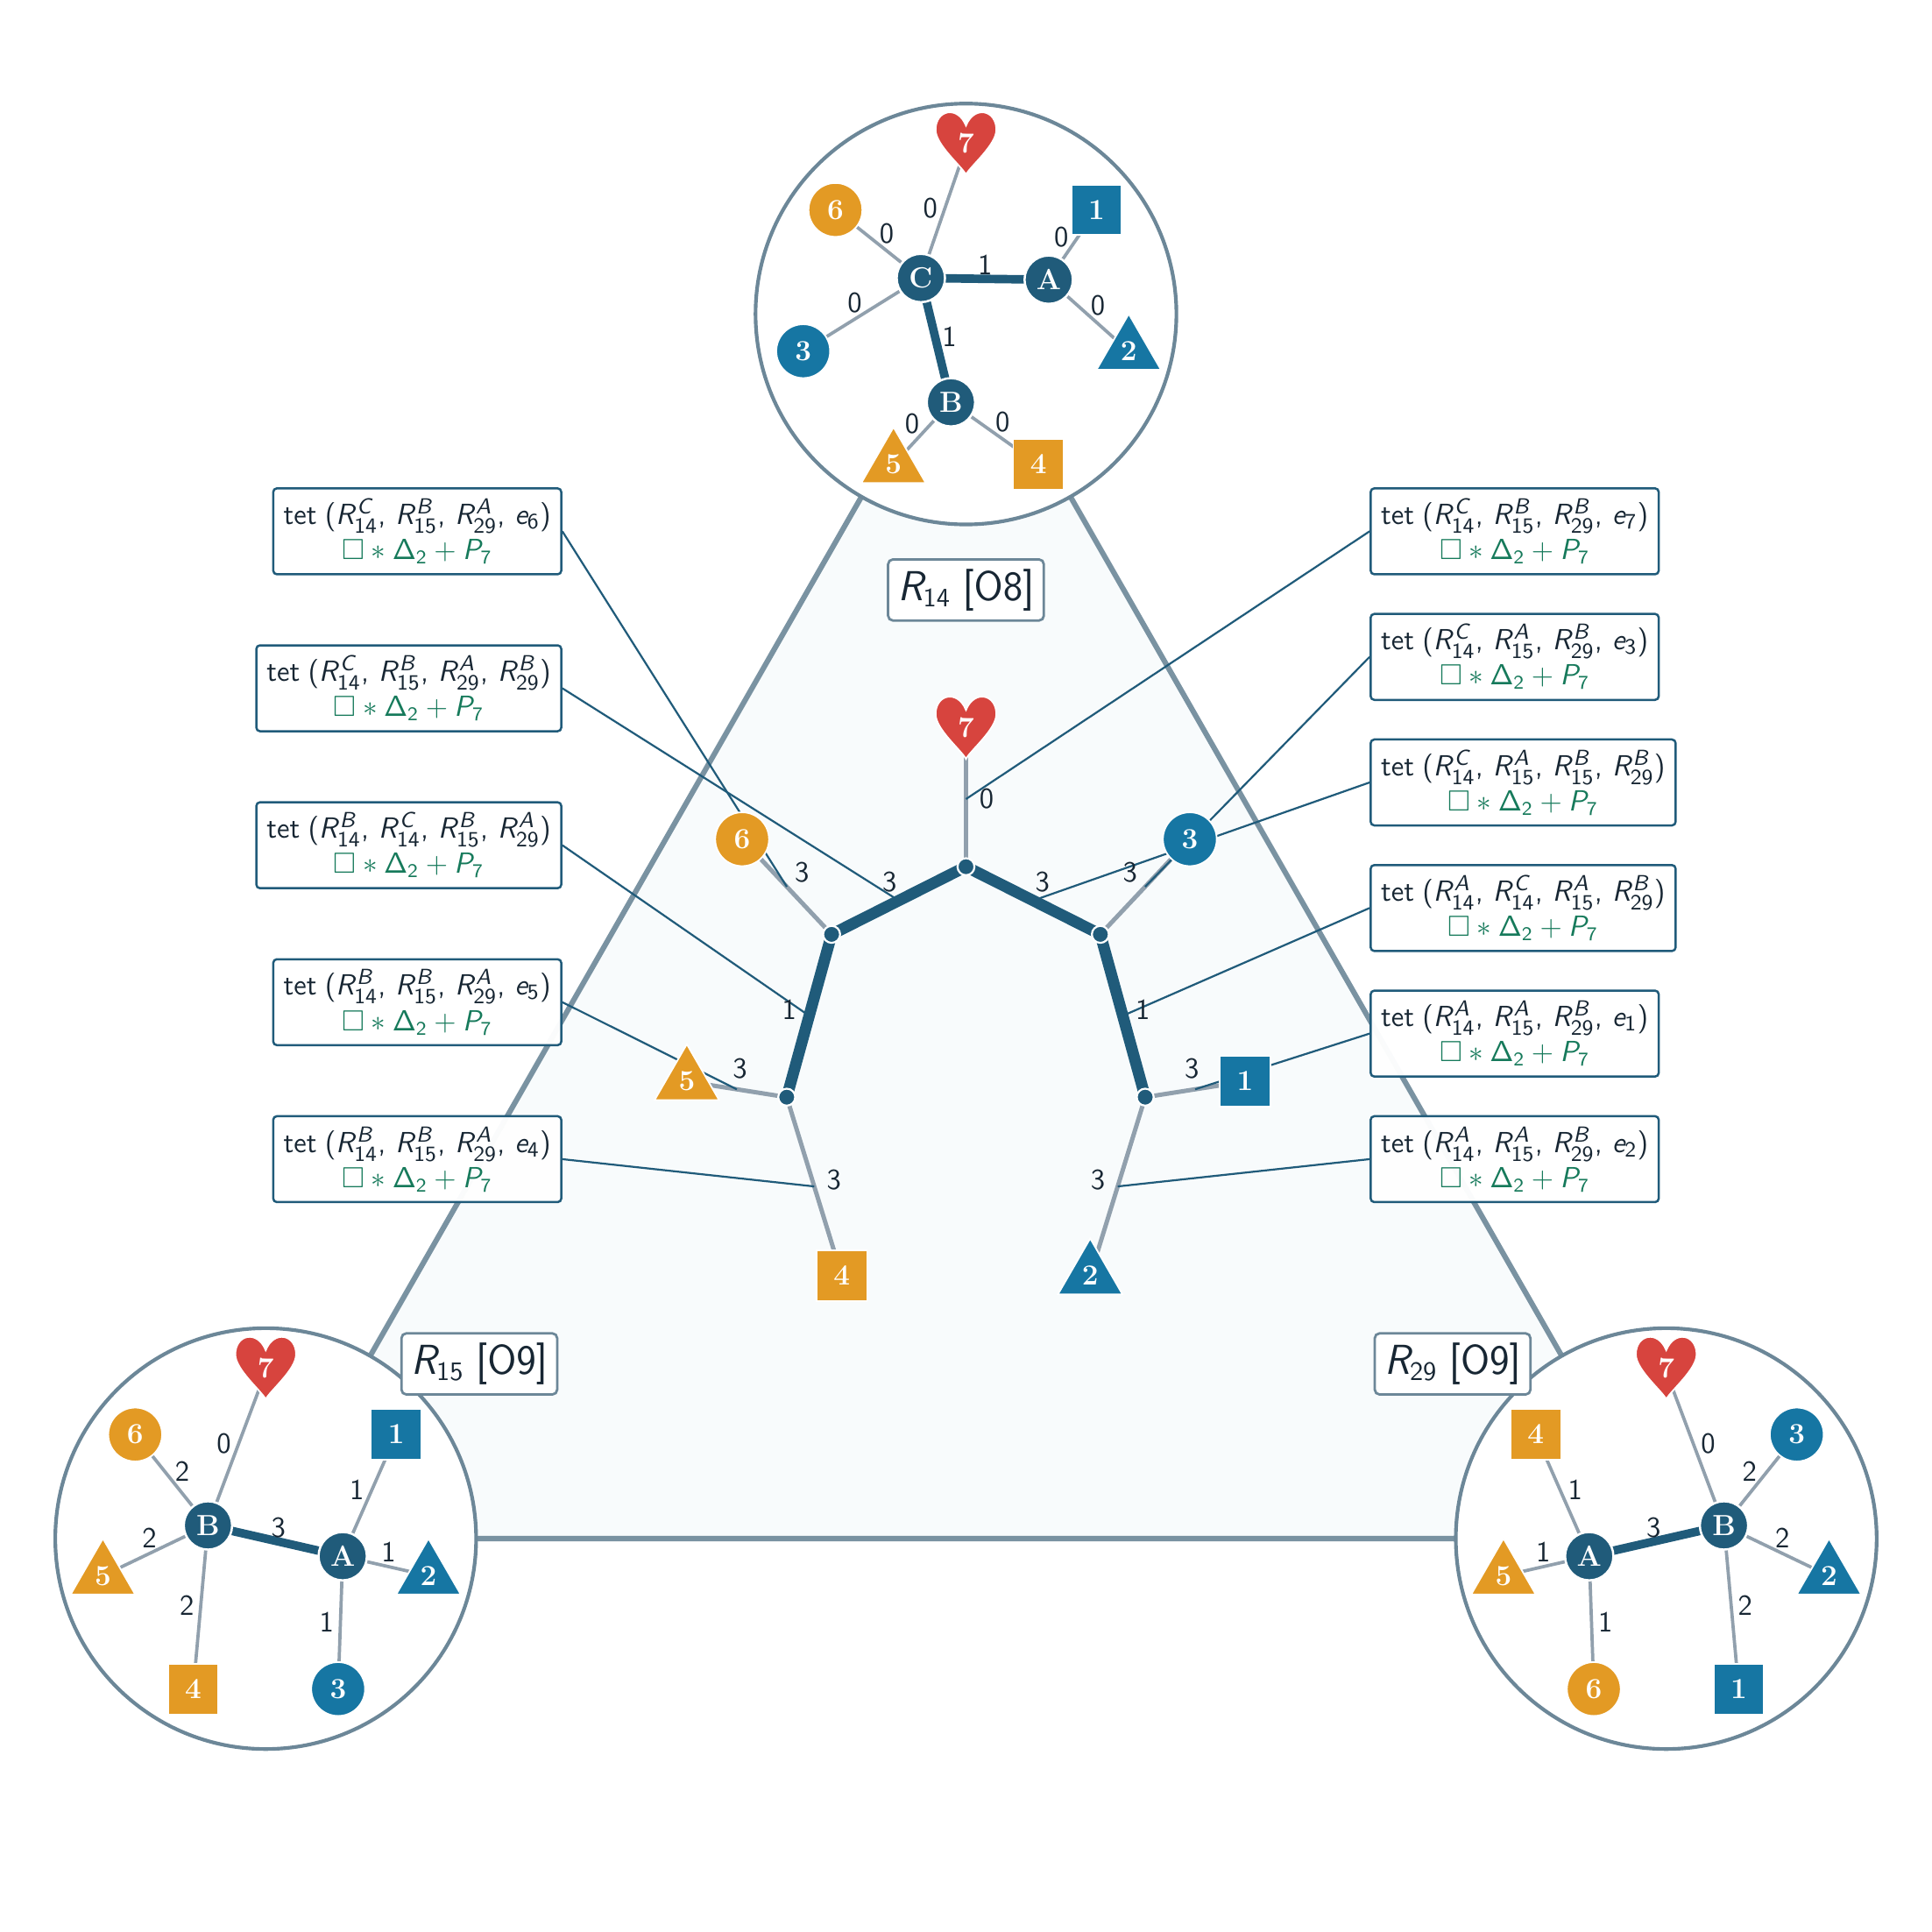
\begin{tikzpicture}[x=1cm,y=1cm]
\path[use as bounding box] (-13.65,-13.65) rectangle (13.65,13.65);
\path[support cell] (0.00000,9.45000)--(-10.15000,-8.30000)--(10.15000,-8.30000)--cycle;
\path[vertex disc] (0.00000,9.45000) circle[radius=3.05000cm];
\path[vertex disc] (-10.15000,-8.30000) circle[radius=3.05000cm];
\path[vertex disc] (10.15000,-8.30000) circle[radius=3.05000cm];
\coordinate (corner-1-v1) at (1.89203,10.95885);
\coordinate (corner-1-v2) at (2.35933,8.91150);
\coordinate (corner-1-v3) at (-2.35933,8.91150);
\coordinate (corner-1-v4) at (1.05000,7.26966);
\coordinate (corner-1-v5) at (-1.05000,7.26966);
\coordinate (corner-1-v6) at (-1.89203,10.95885);
\coordinate (corner-1-v7) at (0.00000,11.87000);
\coordinate (corner-1-v8) at (1.19910,9.94731);
\coordinate (corner-1-v9) at (-0.21802,8.17030);
\coordinate (corner-1-v10) at (-0.65406,9.97159);
\draw[internal edge] (corner-1-v8)--node[mini length,pos=0.5] {\(1\)}(corner-1-v10);
\draw[internal edge] (corner-1-v9)--node[mini length,pos=0.5] {\(1\)}(corner-1-v10);
\draw[pendant edge] (corner-1-v1)--node[mini length,pos=0.5] {\(0\)}(corner-1-v8);
\draw[pendant edge] (corner-1-v2)--node[mini length,pos=0.5] {\(0\)}(corner-1-v8);
\draw[pendant edge] (corner-1-v3)--node[mini length,pos=0.5] {\(0\)}(corner-1-v10);
\draw[pendant edge] (corner-1-v4)--node[mini length,pos=0.5] {\(0\)}(corner-1-v9);
\draw[pendant edge] (corner-1-v5)--node[mini length,pos=0.5] {\(0\)}(corner-1-v9);
\draw[pendant edge] (corner-1-v6)--node[mini length,pos=0.5] {\(0\)}(corner-1-v10);
\draw[pendant edge] (corner-1-v7)--node[mini length,pos=0.5] {\(0\)}(corner-1-v10);
\node[lettered vertex] at (corner-1-v8) {A};
\node[lettered vertex] at (corner-1-v9) {B};
\node[lettered vertex] at (corner-1-v10) {C};
\taxonone{corner-1-v1}
\taxontwo{corner-1-v2}
\taxonthree{corner-1-v3}
\taxonfour{corner-1-v4}
\taxonfive{corner-1-v5}
\taxonsix{corner-1-v6}
\taxonseven{corner-1-v7}
\node[ray title] at (0.00000,5.45000) {\(R_{14}\;[\mathrm{O}8]\)};
\coordinate (corner-2-v1) at (-8.25797,-6.79115);
\coordinate (corner-2-v2) at (-7.79067,-8.83850);
\coordinate (corner-2-v3) at (-9.10000,-10.48034);
\coordinate (corner-2-v4) at (-11.20000,-10.48034);
\coordinate (corner-2-v5) at (-12.50933,-8.83850);
\coordinate (corner-2-v6) at (-12.04203,-6.79115);
\coordinate (corner-2-v7) at (-10.15000,-5.88000);
\coordinate (corner-2-v8) at (-9.03392,-8.55474);
\coordinate (corner-2-v9) at (-10.98706,-8.10895);
\draw[internal edge] (corner-2-v8)--node[mini length,pos=0.5] {\(3\)}(corner-2-v9);
\draw[pendant edge] (corner-2-v1)--node[mini length,pos=0.5] {\(1\)}(corner-2-v8);
\draw[pendant edge] (corner-2-v2)--node[mini length,pos=0.5] {\(1\)}(corner-2-v8);
\draw[pendant edge] (corner-2-v3)--node[mini length,pos=0.5] {\(1\)}(corner-2-v8);
\draw[pendant edge] (corner-2-v4)--node[mini length,pos=0.5] {\(2\)}(corner-2-v9);
\draw[pendant edge] (corner-2-v5)--node[mini length,pos=0.5] {\(2\)}(corner-2-v9);
\draw[pendant edge] (corner-2-v6)--node[mini length,pos=0.5] {\(2\)}(corner-2-v9);
\draw[pendant edge] (corner-2-v7)--node[mini length,pos=0.5] {\(0\)}(corner-2-v9);
\node[lettered vertex] at (corner-2-v8) {A};
\node[lettered vertex] at (corner-2-v9) {B};
\taxonone{corner-2-v1}
\taxontwo{corner-2-v2}
\taxonthree{corner-2-v3}
\taxonfour{corner-2-v4}
\taxonfive{corner-2-v5}
\taxonsix{corner-2-v6}
\taxonseven{corner-2-v7}
\node[ray title] at (-7.05349,-5.76788) {\(R_{15}\;[\mathrm{O}9]\)};
\coordinate (corner-3-v1) at (11.20000,-10.48034);
\coordinate (corner-3-v2) at (12.50933,-8.83850);
\coordinate (corner-3-v3) at (12.04203,-6.79115);
\coordinate (corner-3-v4) at (8.25797,-6.79115);
\coordinate (corner-3-v5) at (7.79067,-8.83850);
\coordinate (corner-3-v6) at (9.10000,-10.48034);
\coordinate (corner-3-v7) at (10.15000,-5.88000);
\coordinate (corner-3-v8) at (9.03392,-8.55474);
\coordinate (corner-3-v9) at (10.98706,-8.10895);
\draw[internal edge] (corner-3-v8)--node[mini length,pos=0.5] {\(3\)}(corner-3-v9);
\draw[pendant edge] (corner-3-v1)--node[mini length,pos=0.5] {\(2\)}(corner-3-v9);
\draw[pendant edge] (corner-3-v2)--node[mini length,pos=0.5] {\(2\)}(corner-3-v9);
\draw[pendant edge] (corner-3-v3)--node[mini length,pos=0.5] {\(2\)}(corner-3-v9);
\draw[pendant edge] (corner-3-v4)--node[mini length,pos=0.5] {\(1\)}(corner-3-v8);
\draw[pendant edge] (corner-3-v5)--node[mini length,pos=0.5] {\(1\)}(corner-3-v8);
\draw[pendant edge] (corner-3-v6)--node[mini length,pos=0.5] {\(1\)}(corner-3-v8);
\draw[pendant edge] (corner-3-v7)--node[mini length,pos=0.5] {\(0\)}(corner-3-v9);
\node[lettered vertex] at (corner-3-v8) {A};
\node[lettered vertex] at (corner-3-v9) {B};
\taxonone{corner-3-v1}
\taxontwo{corner-3-v2}
\taxonthree{corner-3-v3}
\taxonfour{corner-3-v4}
\taxonfive{corner-3-v5}
\taxonsix{corner-3-v6}
\taxonseven{corner-3-v7}
\node[ray title] at (7.05349,-5.76788) {\(R_{29}\;[\mathrm{O}9]\)};
\coordinate (central-v1) at (4.04595,-1.67346);
\coordinate (central-v2) at (1.80062,-4.48902);
\coordinate (central-v3) at (3.24460,1.83748);
\coordinate (central-v4) at (-1.80062,-4.48902);
\coordinate (central-v5) at (-4.04595,-1.67346);
\coordinate (central-v6) at (-3.24460,1.83748);
\coordinate (central-v7) at (0.00000,3.40000);
\coordinate (central-v8) at (2.59804,-1.90139);
\coordinate (central-v9) at (1.94755,0.45833);
\coordinate (central-v10) at (0.00000,1.43889);
\coordinate (central-v11) at (-2.59804,-1.90139);
\coordinate (central-v12) at (-1.94755,0.45833);
\draw[central internal edge] (central-v8)--(central-v9);
\draw[central internal edge] (central-v9)--(central-v10);
\draw[central internal edge] (central-v10)--(central-v12);
\draw[central internal edge] (central-v11)--(central-v12);
\draw[central pendant edge] (central-v1)--(central-v8);
\draw[central pendant edge] (central-v2)--(central-v8);
\draw[central pendant edge] (central-v3)--(central-v9);
\draw[central pendant edge] (central-v4)--(central-v11);
\draw[central pendant edge] (central-v5)--(central-v11);
\draw[central pendant edge] (central-v6)--(central-v12);
\draw[central pendant edge] (central-v7)--(central-v10);
\draw[edge leader] (-5.85000,6.30000)--(-2.59607,1.14791);
\draw[edge leader] (-5.85000,4.02500)--(-0.97377,0.94861);
\draw[edge leader] (-5.85000,1.75000)--(-2.27279,-0.72153);
\draw[edge leader] (-5.85000,-0.52500)--(-3.32199,-1.78742);
\draw[edge leader] (-5.85000,-2.80000)--(-2.19933,-3.19520);
\draw[edge leader] (5.85000,6.30000)--(0.00000,2.41944);
\draw[edge leader] (5.85000,4.48000)--(2.59607,1.14791);
\draw[edge leader] (5.85000,2.66000)--(0.97377,0.94861);
\draw[edge leader] (5.85000,0.84000)--(2.27279,-0.72153);
\draw[edge leader] (5.85000,-0.98000)--(3.32199,-1.78742);
\draw[edge leader] (5.85000,-2.80000)--(2.19933,-3.19520);
\node[internal vertex] at (central-v8) {};
\node[internal vertex] at (central-v9) {};
\node[internal vertex] at (central-v10) {};
\node[internal vertex] at (central-v11) {};
\node[internal vertex] at (central-v12) {};
\taxonone{central-v1}
\taxontwo{central-v2}
\taxonthree{central-v3}
\taxonfour{central-v4}
\taxonfive{central-v5}
\taxonsix{central-v6}
\taxonseven{central-v7}
\path (central-v8)--node[central length,pos=.50] {\(1\)}(central-v9);
\path (central-v9)--node[central length,pos=.50] {\(3\)}(central-v10);
\path (central-v10)--node[central length,pos=.50] {\(3\)}(central-v12);
\path (central-v11)--node[central length,pos=.50] {\(1\)}(central-v12);
\path (central-v1)--node[central length,pos=.50] {\(3\)}(central-v8);
\path (central-v2)--node[central length,pos=.50] {\(3\)}(central-v8);
\path (central-v3)--node[central length,pos=.50] {\(3\)}(central-v9);
\path (central-v4)--node[central length,pos=.50] {\(3\)}(central-v11);
\path (central-v5)--node[central length,pos=.50] {\(3\)}(central-v11);
\path (central-v6)--node[central length,pos=.50] {\(3\)}(central-v12);
\path (central-v7)--node[central length,pos=.50] {\(0\)}(central-v10);
\node[edge callout,anchor=east] (callout-1) at (-5.85000,6.30000) {\(\mathrm{tet}\;(R_{14}^{C},\,R_{15}^{B},\,R_{29}^{A},\,e_{6})\)\\{\fontsize{12}{14}\selectfont\color{toricgreen}\(\square\ast\Delta_{2}+P_{7}\)}};
\node[edge callout,anchor=east] (callout-2) at (-5.85000,4.02500) {\(\mathrm{tet}\;(R_{14}^{C},\,R_{15}^{B},\,R_{29}^{A},\,R_{29}^{B})\)\\{\fontsize{12}{14}\selectfont\color{toricgreen}\(\square\ast\Delta_{2}+P_{7}\)}};
\node[edge callout,anchor=east] (callout-3) at (-5.85000,1.75000) {\(\mathrm{tet}\;(R_{14}^{B},\,R_{14}^{C},\,R_{15}^{B},\,R_{29}^{A})\)\\{\fontsize{12}{14}\selectfont\color{toricgreen}\(\square\ast\Delta_{2}+P_{7}\)}};
\node[edge callout,anchor=east] (callout-4) at (-5.85000,-0.52500) {\(\mathrm{tet}\;(R_{14}^{B},\,R_{15}^{B},\,R_{29}^{A},\,e_{5})\)\\{\fontsize{12}{14}\selectfont\color{toricgreen}\(\square\ast\Delta_{2}+P_{7}\)}};
\node[edge callout,anchor=east] (callout-5) at (-5.85000,-2.80000) {\(\mathrm{tet}\;(R_{14}^{B},\,R_{15}^{B},\,R_{29}^{A},\,e_{4})\)\\{\fontsize{12}{14}\selectfont\color{toricgreen}\(\square\ast\Delta_{2}+P_{7}\)}};
\node[edge callout,anchor=west] (callout-6) at (5.85000,6.30000) {\(\mathrm{tet}\;(R_{14}^{C},\,R_{15}^{B},\,R_{29}^{B},\,e_{7})\)\\{\fontsize{12}{14}\selectfont\color{toricgreen}\(\square\ast\Delta_{2}+P_{7}\)}};
\node[edge callout,anchor=west] (callout-7) at (5.85000,4.48000) {\(\mathrm{tet}\;(R_{14}^{C},\,R_{15}^{A},\,R_{29}^{B},\,e_{3})\)\\{\fontsize{12}{14}\selectfont\color{toricgreen}\(\square\ast\Delta_{2}+P_{7}\)}};
\node[edge callout,anchor=west] (callout-8) at (5.85000,2.66000) {\(\mathrm{tet}\;(R_{14}^{C},\,R_{15}^{A},\,R_{15}^{B},\,R_{29}^{B})\)\\{\fontsize{12}{14}\selectfont\color{toricgreen}\(\square\ast\Delta_{2}+P_{7}\)}};
\node[edge callout,anchor=west] (callout-9) at (5.85000,0.84000) {\(\mathrm{tet}\;(R_{14}^{A},\,R_{14}^{C},\,R_{15}^{A},\,R_{29}^{B})\)\\{\fontsize{12}{14}\selectfont\color{toricgreen}\(\square\ast\Delta_{2}+P_{7}\)}};
\node[edge callout,anchor=west] (callout-10) at (5.85000,-0.98000) {\(\mathrm{tet}\;(R_{14}^{A},\,R_{15}^{A},\,R_{29}^{B},\,e_{1})\)\\{\fontsize{12}{14}\selectfont\color{toricgreen}\(\square\ast\Delta_{2}+P_{7}\)}};
\node[edge callout,anchor=west] (callout-11) at (5.85000,-2.80000) {\(\mathrm{tet}\;(R_{14}^{A},\,R_{15}^{A},\,R_{29}^{B},\,e_{2})\)\\{\fontsize{12}{14}\selectfont\color{toricgreen}\(\square\ast\Delta_{2}+P_{7}\)}};
\end{tikzpicture}\end{center}\vspace{-1mm}
\begin{atlasbox}\begin{atlaspanel}
\textcolor{toricgreen}{\bfseries PRIME TORIC}\quad \(P_{7}\):\enspace \(\mathrm{Wed}(\mathrm{Wed}(\square\ast\Delta_{0};\,\Delta_1);\,\Delta_2)\)\quad \(f=(13,38,48,30,9)\)\quad 14 lattice points
\end{atlaspanel}\end{atlasbox}
\clearpage
\begin{atlaspanel}[top=1mm,bottom=2mm]
\AtlasSupportOrbitSplit{%
\vspace*{-3mm}\mbox{{\LARGE\bfseries Triangle orbit 8}\hspace{3mm}\raisebox{.8mm}[0pt][0pt]{{\fontsize{16}{18}\selectfont\color{muted}size 12}}}%
}{%
\vspace*{-3mm}{\fontsize{13}{16}\selectfont{\color{muted}\(\mathbb{Q}\) and \(\mathbb{F}_2\)}\quad{\color{muted}\(\underline{\{1,\,2,\,6\}}\), \(\{2,\,4,\,7\}\), \(\{23,\,25,\,40\}\), \(\{24,\,26,\,41\}\), \(\{28,\,41,\,42\}\), \(\{28,\,40,\,43\}\), \(\{11,\,25,\,48\}\), \(\{12,\,26,\,49\}\), \(\{12,\,32,\,38\}\), \(\{11,\,31,\,39\}\), \(\{6,\,32,\,50\}\), \(\{7,\,31,\,51\}\)}\rule[-3mm]{0pt}{3mm}}%
}%
\end{atlaspanel}\vspace{2mm}
\begin{center}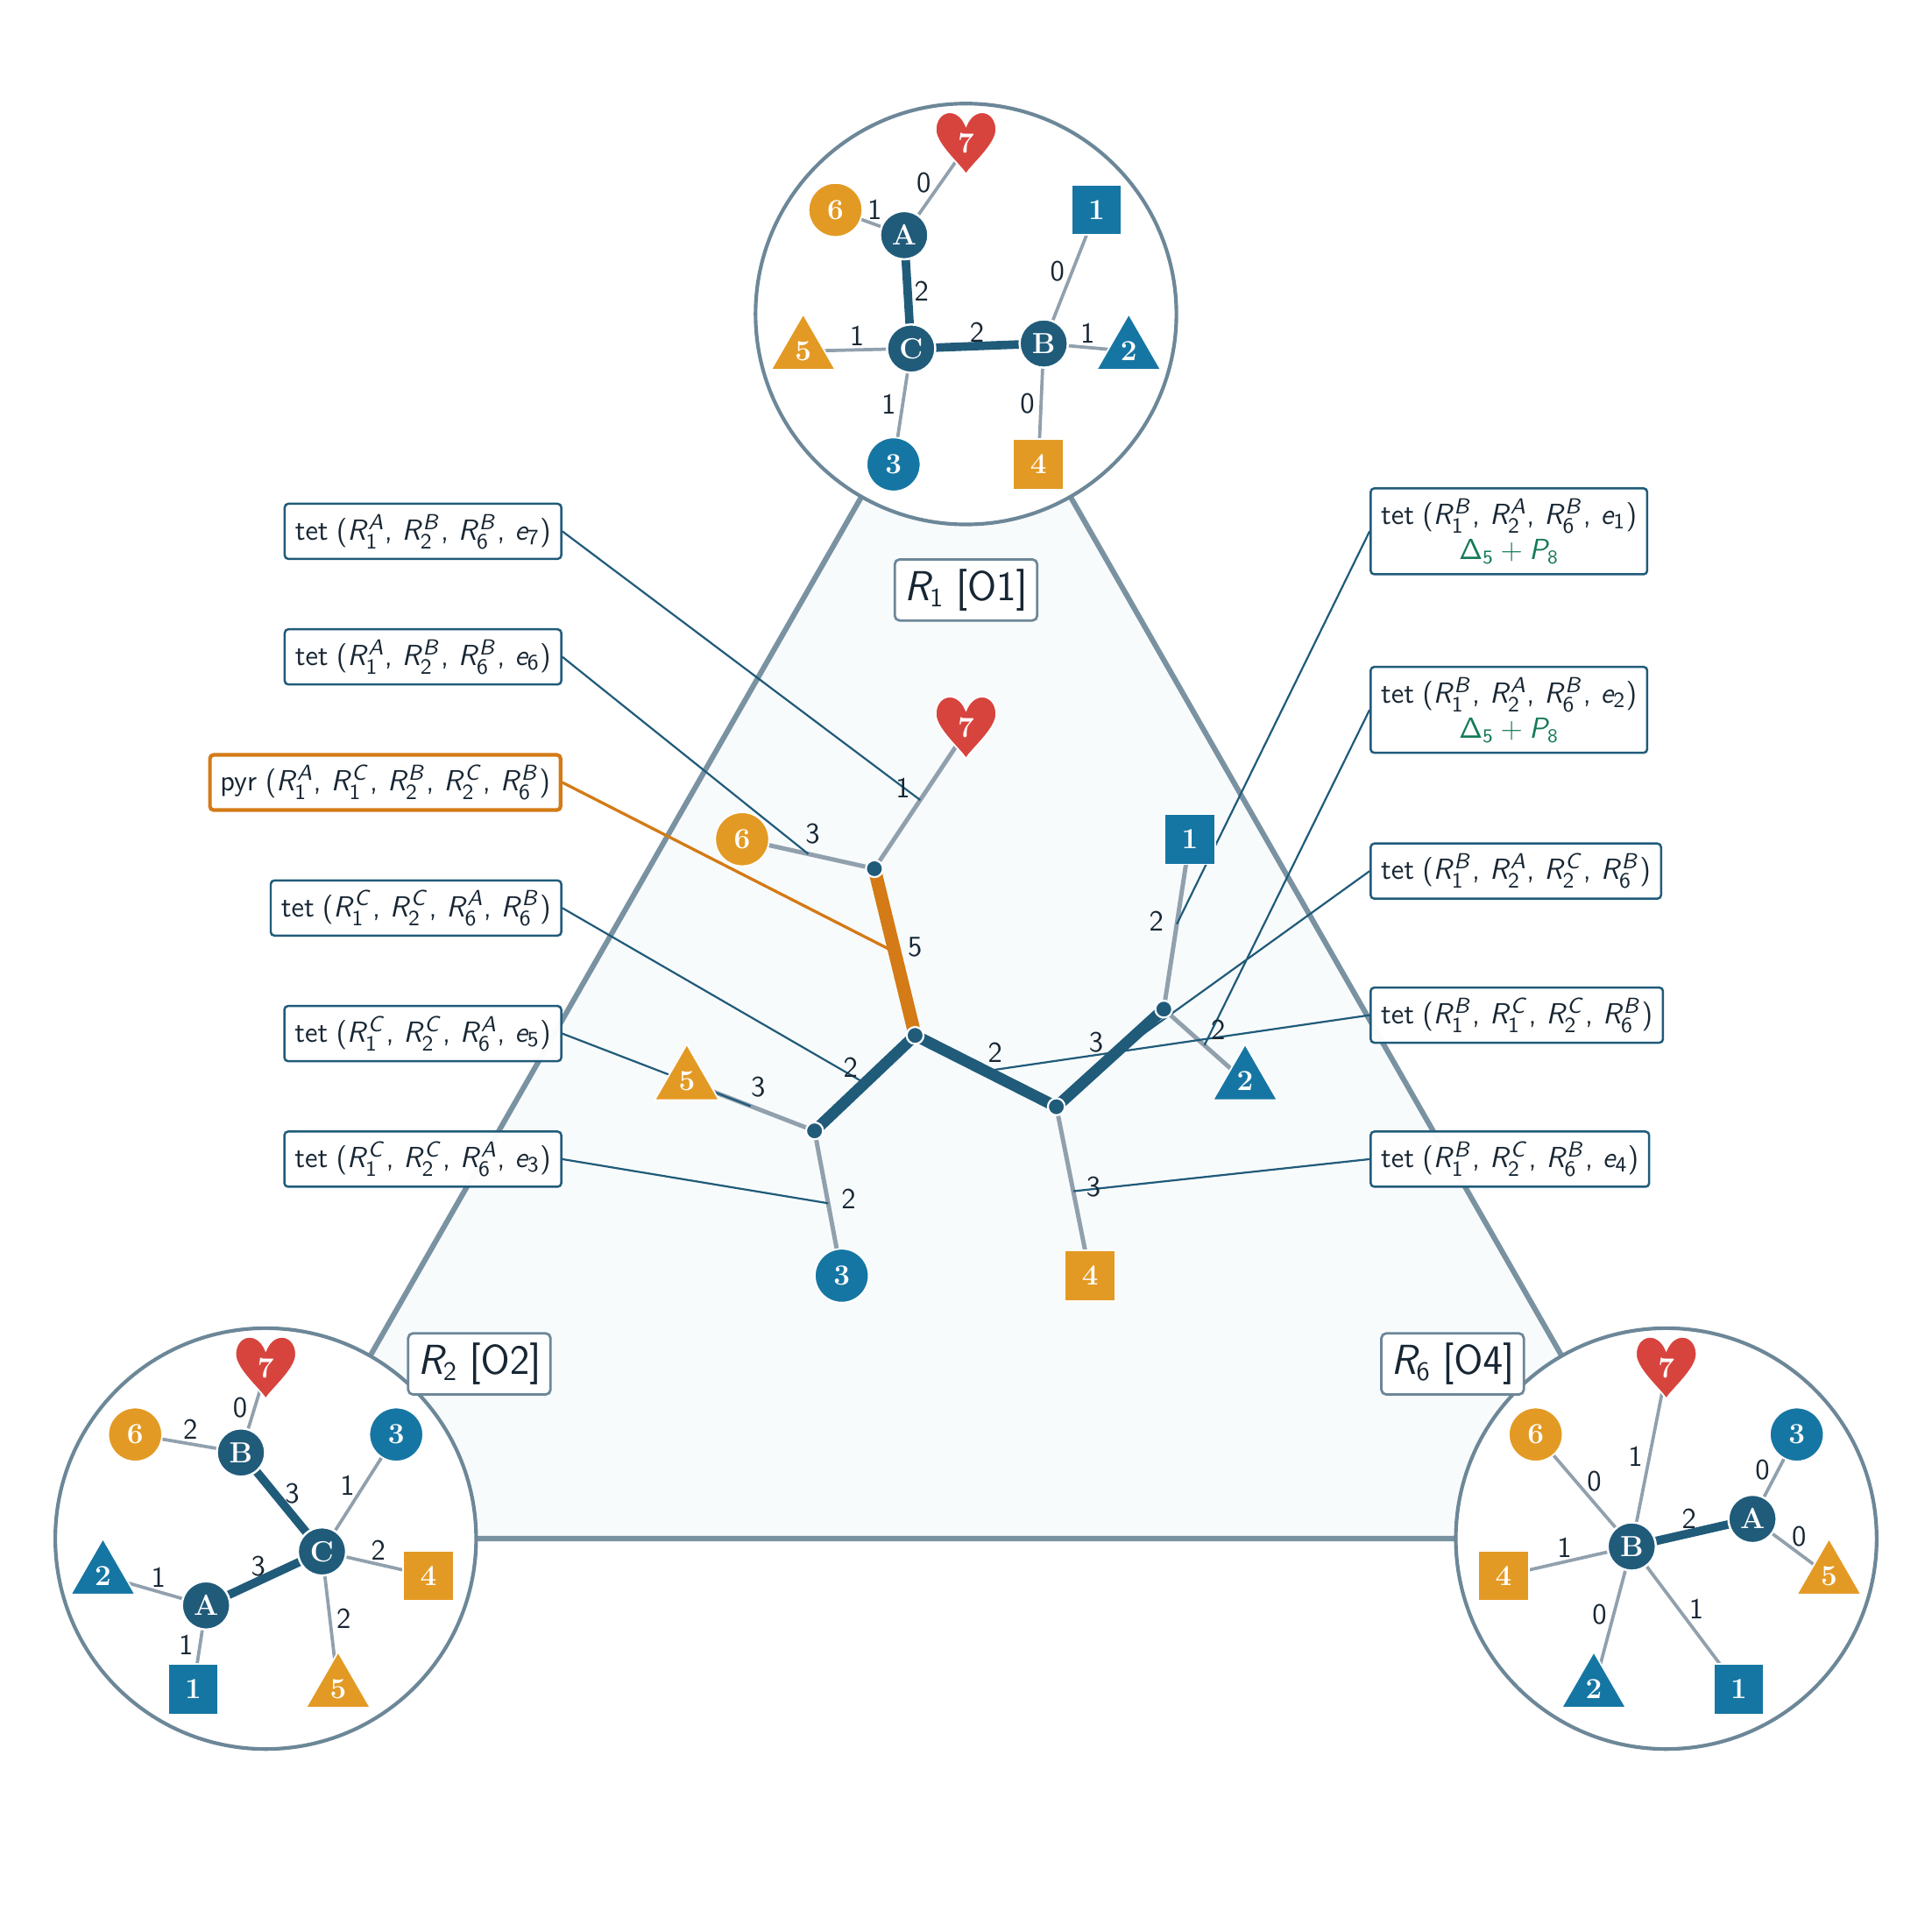
\begin{tikzpicture}[x=1cm,y=1cm]
\path[use as bounding box] (-13.65,-13.65) rectangle (13.65,13.65);
\path[support cell] (0.00000,9.45000)--(-10.15000,-8.30000)--(10.15000,-8.30000)--cycle;
\path[vertex disc] (0.00000,9.45000) circle[radius=3.05000cm];
\path[vertex disc] (-10.15000,-8.30000) circle[radius=3.05000cm];
\path[vertex disc] (10.15000,-8.30000) circle[radius=3.05000cm];
\coordinate (corner-1-v1) at (1.89203,10.95885);
\coordinate (corner-1-v2) at (2.35933,8.91150);
\coordinate (corner-1-v3) at (-1.05000,7.26966);
\coordinate (corner-1-v4) at (1.05000,7.26966);
\coordinate (corner-1-v5) at (-2.35933,8.91150);
\coordinate (corner-1-v6) at (-1.89203,10.95885);
\coordinate (corner-1-v7) at (0.00000,11.87000);
\coordinate (corner-1-v8) at (-0.89552,10.59262);
\coordinate (corner-1-v9) at (1.12671,9.02225);
\coordinate (corner-1-v10) at (-0.79454,8.94901);
\draw[internal edge] (corner-1-v8)--node[mini length,pos=0.5] {\(2\)}(corner-1-v10);
\draw[internal edge] (corner-1-v9)--node[mini length,pos=0.5] {\(2\)}(corner-1-v10);
\draw[pendant edge] (corner-1-v1)--node[mini length,pos=0.5] {\(0\)}(corner-1-v9);
\draw[pendant edge] (corner-1-v2)--node[mini length,pos=0.5] {\(1\)}(corner-1-v9);
\draw[pendant edge] (corner-1-v3)--node[mini length,pos=0.5] {\(1\)}(corner-1-v10);
\draw[pendant edge] (corner-1-v4)--node[mini length,pos=0.5] {\(0\)}(corner-1-v9);
\draw[pendant edge] (corner-1-v5)--node[mini length,pos=0.5] {\(1\)}(corner-1-v10);
\draw[pendant edge] (corner-1-v6)--node[mini length,pos=0.5] {\(1\)}(corner-1-v8);
\draw[pendant edge] (corner-1-v7)--node[mini length,pos=0.5] {\(0\)}(corner-1-v8);
\node[lettered vertex] at (corner-1-v8) {A};
\node[lettered vertex] at (corner-1-v9) {B};
\node[lettered vertex] at (corner-1-v10) {C};
\taxonone{corner-1-v1}
\taxontwo{corner-1-v2}
\taxonthree{corner-1-v3}
\taxonfour{corner-1-v4}
\taxonfive{corner-1-v5}
\taxonsix{corner-1-v6}
\taxonseven{corner-1-v7}
\node[ray title] at (0.00000,5.45000) {\(R_{1}\;[\mathrm{O}1]\)};
\coordinate (corner-2-v1) at (-11.20000,-10.48034);
\coordinate (corner-2-v2) at (-12.50933,-8.83850);
\coordinate (corner-2-v3) at (-8.25797,-6.79115);
\coordinate (corner-2-v4) at (-7.79067,-8.83850);
\coordinate (corner-2-v5) at (-9.10000,-10.48034);
\coordinate (corner-2-v6) at (-12.04203,-6.79115);
\coordinate (corner-2-v7) at (-10.15000,-5.88000);
\coordinate (corner-2-v8) at (-11.01458,-9.26833);
\coordinate (corner-2-v9) at (-10.50881,-7.05244);
\coordinate (corner-2-v10) at (-9.33441,-8.48615);
\draw[internal edge] (corner-2-v8)--node[mini length,pos=0.5] {\(3\)}(corner-2-v10);
\draw[internal edge] (corner-2-v9)--node[mini length,pos=0.5] {\(3\)}(corner-2-v10);
\draw[pendant edge] (corner-2-v1)--node[mini length,pos=0.5] {\(1\)}(corner-2-v8);
\draw[pendant edge] (corner-2-v2)--node[mini length,pos=0.5] {\(1\)}(corner-2-v8);
\draw[pendant edge] (corner-2-v3)--node[mini length,pos=0.5] {\(1\)}(corner-2-v10);
\draw[pendant edge] (corner-2-v4)--node[mini length,pos=0.5] {\(2\)}(corner-2-v10);
\draw[pendant edge] (corner-2-v5)--node[mini length,pos=0.5] {\(2\)}(corner-2-v10);
\draw[pendant edge] (corner-2-v6)--node[mini length,pos=0.5] {\(2\)}(corner-2-v9);
\draw[pendant edge] (corner-2-v7)--node[mini length,pos=0.5] {\(0\)}(corner-2-v9);
\node[lettered vertex] at (corner-2-v8) {A};
\node[lettered vertex] at (corner-2-v9) {B};
\node[lettered vertex] at (corner-2-v10) {C};
\taxonone{corner-2-v1}
\taxontwo{corner-2-v2}
\taxonthree{corner-2-v3}
\taxonfour{corner-2-v4}
\taxonfive{corner-2-v5}
\taxonsix{corner-2-v6}
\taxonseven{corner-2-v7}
\node[ray title] at (-7.05349,-5.76788) {\(R_{2}\;[\mathrm{O}2]\)};
\coordinate (corner-3-v1) at (11.20000,-10.48034);
\coordinate (corner-3-v2) at (9.10000,-10.48034);
\coordinate (corner-3-v3) at (12.04203,-6.79115);
\coordinate (corner-3-v4) at (7.79067,-8.83850);
\coordinate (corner-3-v5) at (12.50933,-8.83850);
\coordinate (corner-3-v6) at (8.25797,-6.79115);
\coordinate (corner-3-v7) at (10.15000,-5.88000);
\coordinate (corner-3-v8) at (11.40040,-8.01460);
\coordinate (corner-3-v9) at (9.64984,-8.41416);
\draw[internal edge] (corner-3-v8)--node[mini length,pos=0.5] {\(2\)}(corner-3-v9);
\draw[pendant edge] (corner-3-v1)--node[mini length,pos=0.5] {\(1\)}(corner-3-v9);
\draw[pendant edge] (corner-3-v2)--node[mini length,pos=0.5] {\(0\)}(corner-3-v9);
\draw[pendant edge] (corner-3-v3)--node[mini length,pos=0.5] {\(0\)}(corner-3-v8);
\draw[pendant edge] (corner-3-v4)--node[mini length,pos=0.5] {\(1\)}(corner-3-v9);
\draw[pendant edge] (corner-3-v5)--node[mini length,pos=0.5] {\(0\)}(corner-3-v8);
\draw[pendant edge] (corner-3-v6)--node[mini length,pos=0.5] {\(0\)}(corner-3-v9);
\draw[pendant edge] (corner-3-v7)--node[mini length,pos=0.5] {\(1\)}(corner-3-v9);
\node[lettered vertex] at (corner-3-v8) {A};
\node[lettered vertex] at (corner-3-v9) {B};
\taxonone{corner-3-v1}
\taxontwo{corner-3-v2}
\taxonthree{corner-3-v3}
\taxonfour{corner-3-v4}
\taxonfive{corner-3-v5}
\taxonsix{corner-3-v6}
\taxonseven{corner-3-v7}
\node[ray title] at (7.05349,-5.76788) {\(R_{6}\;[\mathrm{O}4]\)};
\coordinate (central-v1) at (3.24460,1.83748);
\coordinate (central-v2) at (4.04595,-1.67346);
\coordinate (central-v3) at (-1.80062,-4.48902);
\coordinate (central-v4) at (1.80062,-4.48902);
\coordinate (central-v5) at (-4.04595,-1.67346);
\coordinate (central-v6) at (-3.24460,1.83748);
\coordinate (central-v7) at (0.00000,3.40000);
\coordinate (central-v8) at (-1.32729,1.41030);
\coordinate (central-v9) at (2.86687,-0.62544);
\coordinate (central-v10) at (-2.19462,-2.38969);
\coordinate (central-v11) at (1.31007,-2.04035);
\coordinate (central-v12) at (-0.73728,-1.00658);
\draw[central pyramid edge] (central-v8)--(central-v12);
\draw[central internal edge] (central-v9)--(central-v11);
\draw[central internal edge] (central-v10)--(central-v12);
\draw[central internal edge] (central-v11)--(central-v12);
\draw[central pendant edge] (central-v1)--(central-v9);
\draw[central pendant edge] (central-v2)--(central-v9);
\draw[central pendant edge] (central-v3)--(central-v10);
\draw[central pendant edge] (central-v4)--(central-v11);
\draw[central pendant edge] (central-v5)--(central-v10);
\draw[central pendant edge] (central-v6)--(central-v8);
\draw[central pendant edge] (central-v7)--(central-v8);
\draw[edge leader] (-5.85000,6.30000)--(-0.66365,2.40515);
\draw[edge leader] (-5.85000,4.48000)--(-2.28595,1.62389);
\draw[pyramid leader] (-5.85000,2.66000)--(-1.03229,0.20186);
\draw[edge leader] (-5.85000,0.84000)--(-1.46595,-1.69813);
\draw[edge leader] (-5.85000,-0.98000)--(-3.12028,-2.03157);
\draw[edge leader] (-5.85000,-2.80000)--(-1.99762,-3.43935);
\draw[edge leader] (5.85000,6.30000)--(3.05574,0.60602);
\draw[edge leader] (5.85000,3.71250)--(3.45641,-1.14945);
\draw[edge leader] (5.85000,1.37500)--(2.08847,-1.33289);
\draw[edge leader] (5.85000,-0.71250)--(0.28640,-1.52346);
\draw[edge leader] (5.85000,-2.80000)--(1.55534,-3.26468);
\node[internal vertex] at (central-v8) {};
\node[internal vertex] at (central-v9) {};
\node[internal vertex] at (central-v10) {};
\node[internal vertex] at (central-v11) {};
\node[internal vertex] at (central-v12) {};
\taxonone{central-v1}
\taxontwo{central-v2}
\taxonthree{central-v3}
\taxonfour{central-v4}
\taxonfive{central-v5}
\taxonsix{central-v6}
\taxonseven{central-v7}
\path (central-v8)--node[central length,pos=.50] {\(5\)}(central-v12);
\path (central-v9)--node[central length,pos=.50] {\(3\)}(central-v11);
\path (central-v10)--node[central length,pos=.50] {\(2\)}(central-v12);
\path (central-v11)--node[central length,pos=.50] {\(2\)}(central-v12);
\path (central-v1)--node[central length,pos=.50] {\(2\)}(central-v9);
\path (central-v2)--node[central length,pos=.50] {\(2\)}(central-v9);
\path (central-v3)--node[central length,pos=.50] {\(2\)}(central-v10);
\path (central-v4)--node[central length,pos=.50] {\(3\)}(central-v11);
\path (central-v5)--node[central length,pos=.50] {\(3\)}(central-v10);
\path (central-v6)--node[central length,pos=.50] {\(3\)}(central-v8);
\path (central-v7)--node[central length,pos=.50] {\(1\)}(central-v8);
\node[edge callout,anchor=east] (callout-1) at (-5.85000,6.30000) {\(\mathrm{tet}\;(R_{1}^{A},\,R_{2}^{B},\,R_{6}^{B},\,e_{7})\)};
\node[edge callout,anchor=east] (callout-2) at (-5.85000,4.48000) {\(\mathrm{tet}\;(R_{1}^{A},\,R_{2}^{B},\,R_{6}^{B},\,e_{6})\)};
\node[pyramid callout,anchor=east] (callout-3) at (-5.85000,2.66000) {\(\mathrm{pyr}\;(R_{1}^{A},\,R_{1}^{C},\,R_{2}^{B},\,R_{2}^{C},\,R_{6}^{B})\)};
\node[edge callout,anchor=east] (callout-4) at (-5.85000,0.84000) {\(\mathrm{tet}\;(R_{1}^{C},\,R_{2}^{C},\,R_{6}^{A},\,R_{6}^{B})\)};
\node[edge callout,anchor=east] (callout-5) at (-5.85000,-0.98000) {\(\mathrm{tet}\;(R_{1}^{C},\,R_{2}^{C},\,R_{6}^{A},\,e_{5})\)};
\node[edge callout,anchor=east] (callout-6) at (-5.85000,-2.80000) {\(\mathrm{tet}\;(R_{1}^{C},\,R_{2}^{C},\,R_{6}^{A},\,e_{3})\)};
\node[edge callout,anchor=west] (callout-7) at (5.85000,6.30000) {\(\mathrm{tet}\;(R_{1}^{B},\,R_{2}^{A},\,R_{6}^{B},\,e_{1})\)\\{\fontsize{12}{14}\selectfont\color{toricgreen}\(\Delta_{5}+P_{8}\)}};
\node[edge callout,anchor=west] (callout-8) at (5.85000,3.71250) {\(\mathrm{tet}\;(R_{1}^{B},\,R_{2}^{A},\,R_{6}^{B},\,e_{2})\)\\{\fontsize{12}{14}\selectfont\color{toricgreen}\(\Delta_{5}+P_{8}\)}};
\node[edge callout,anchor=west] (callout-9) at (5.85000,1.37500) {\(\mathrm{tet}\;(R_{1}^{B},\,R_{2}^{A},\,R_{2}^{C},\,R_{6}^{B})\)};
\node[edge callout,anchor=west] (callout-10) at (5.85000,-0.71250) {\(\mathrm{tet}\;(R_{1}^{B},\,R_{1}^{C},\,R_{2}^{C},\,R_{6}^{B})\)};
\node[edge callout,anchor=west] (callout-11) at (5.85000,-2.80000) {\(\mathrm{tet}\;(R_{1}^{B},\,R_{2}^{C},\,R_{6}^{B},\,e_{4})\)};
\end{tikzpicture}\end{center}\vspace{-1mm}
\begin{atlasbox}\begin{atlaspanel}
\textcolor{toricgreen}{\bfseries PRIME TORIC}\quad \(P_{8}\):\enspace \(\mathrm{M}(3,5)\ast\Delta_{1}\)\quad \(f=(8,23,32,23,8)\)\quad 15 lattice points
\end{atlaspanel}\end{atlasbox}
\clearpage
\begin{atlaspanel}[top=1mm,bottom=2mm]
\AtlasSupportOrbitSplit{%
\vspace*{-3mm}\mbox{{\LARGE\bfseries Triangle orbit 9}\hspace{3mm}\raisebox{.8mm}[0pt][0pt]{{\fontsize{16}{18}\selectfont\color{muted}size 12}}}%
}{%
\vspace*{-3mm}{\fontsize{13}{16}\selectfont{\color{muted}\(\mathbb{Q}\) and \(\mathbb{F}_2\)}\quad{\color{muted}\(\underline{\{1,\,6,\,9\}}\), \(\{4,\,7,\,10\}\), \(\{9,\,23,\,40\}\), \(\{10,\,24,\,41\}\), \(\{12,\,30,\,38\}\), \(\{10,\,41,\,42\}\), \(\{9,\,40,\,43\}\), \(\{11,\,30,\,39\}\), \(\{11,\,30,\,48\}\), \(\{12,\,30,\,49\}\), \(\{6,\,9,\,50\}\), \(\{7,\,10,\,51\}\)}\rule[-3mm]{0pt}{3mm}}%
}%
\end{atlaspanel}\vspace{2mm}
\begin{center}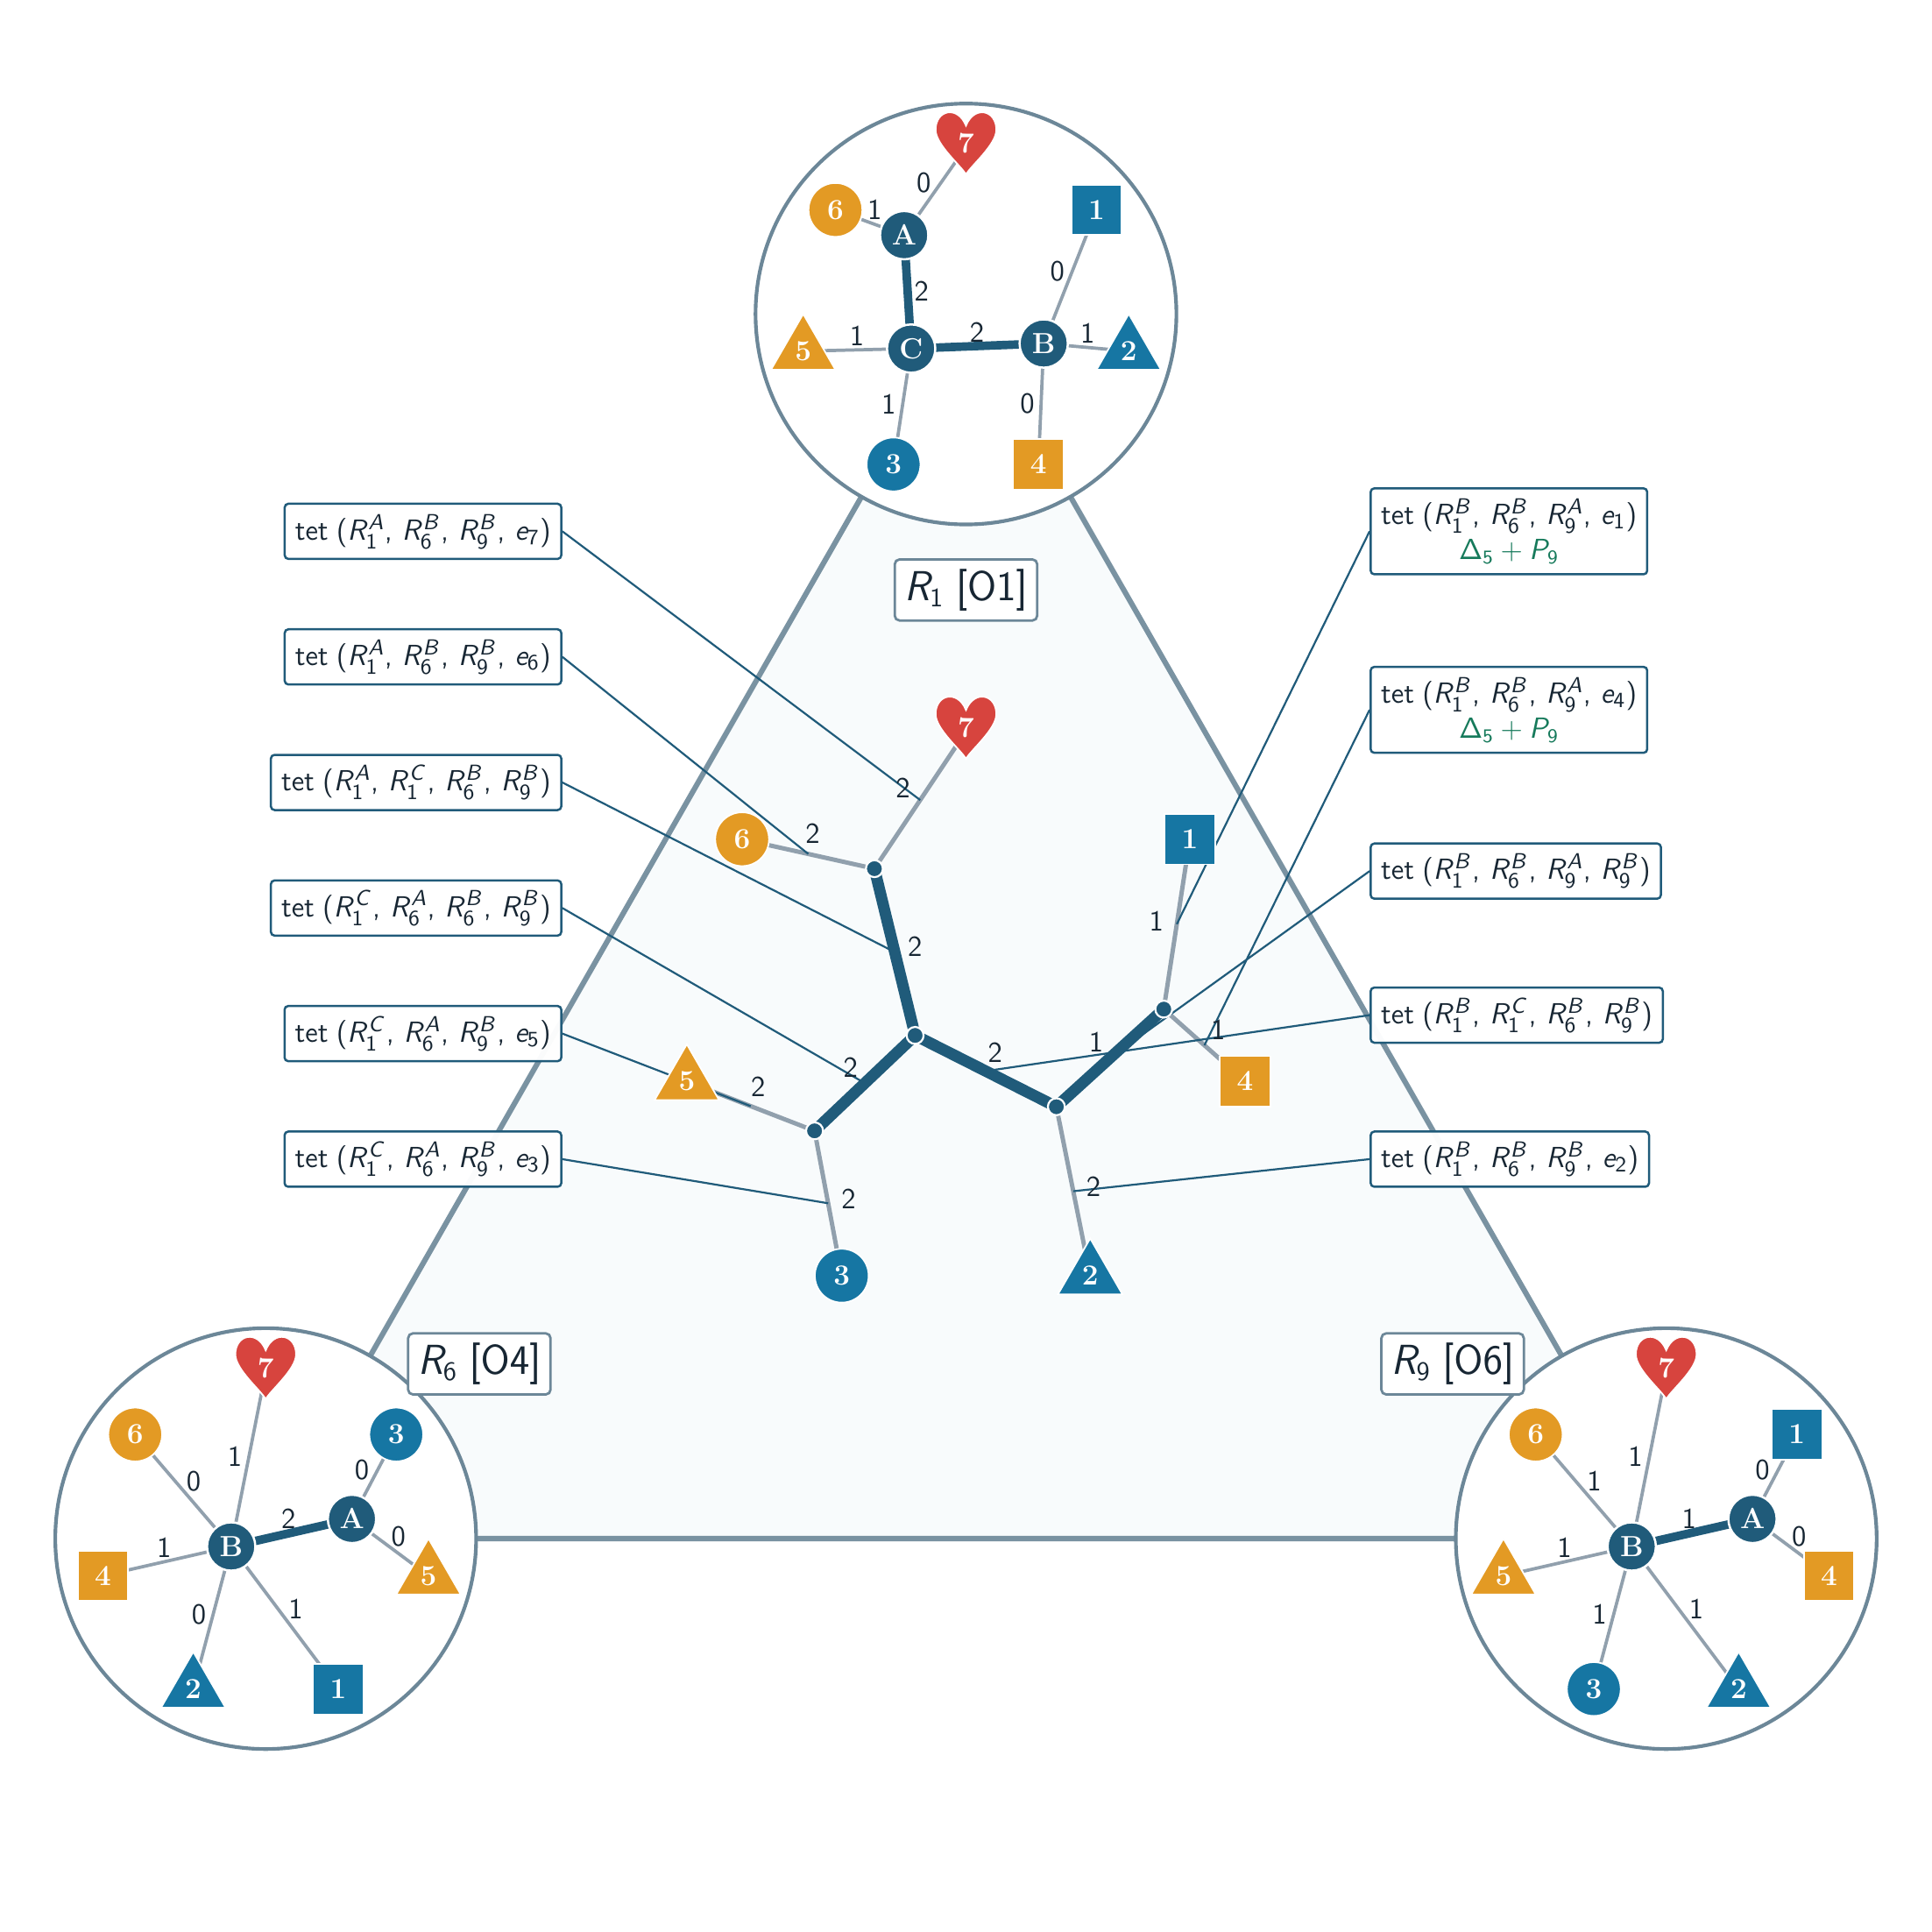
\begin{tikzpicture}[x=1cm,y=1cm]
\path[use as bounding box] (-13.65,-13.65) rectangle (13.65,13.65);
\path[support cell] (0.00000,9.45000)--(-10.15000,-8.30000)--(10.15000,-8.30000)--cycle;
\path[vertex disc] (0.00000,9.45000) circle[radius=3.05000cm];
\path[vertex disc] (-10.15000,-8.30000) circle[radius=3.05000cm];
\path[vertex disc] (10.15000,-8.30000) circle[radius=3.05000cm];
\coordinate (corner-1-v1) at (1.89203,10.95885);
\coordinate (corner-1-v2) at (2.35933,8.91150);
\coordinate (corner-1-v3) at (-1.05000,7.26966);
\coordinate (corner-1-v4) at (1.05000,7.26966);
\coordinate (corner-1-v5) at (-2.35933,8.91150);
\coordinate (corner-1-v6) at (-1.89203,10.95885);
\coordinate (corner-1-v7) at (0.00000,11.87000);
\coordinate (corner-1-v8) at (-0.89552,10.59262);
\coordinate (corner-1-v9) at (1.12671,9.02225);
\coordinate (corner-1-v10) at (-0.79454,8.94901);
\draw[internal edge] (corner-1-v8)--node[mini length,pos=0.5] {\(2\)}(corner-1-v10);
\draw[internal edge] (corner-1-v9)--node[mini length,pos=0.5] {\(2\)}(corner-1-v10);
\draw[pendant edge] (corner-1-v1)--node[mini length,pos=0.5] {\(0\)}(corner-1-v9);
\draw[pendant edge] (corner-1-v2)--node[mini length,pos=0.5] {\(1\)}(corner-1-v9);
\draw[pendant edge] (corner-1-v3)--node[mini length,pos=0.5] {\(1\)}(corner-1-v10);
\draw[pendant edge] (corner-1-v4)--node[mini length,pos=0.5] {\(0\)}(corner-1-v9);
\draw[pendant edge] (corner-1-v5)--node[mini length,pos=0.5] {\(1\)}(corner-1-v10);
\draw[pendant edge] (corner-1-v6)--node[mini length,pos=0.5] {\(1\)}(corner-1-v8);
\draw[pendant edge] (corner-1-v7)--node[mini length,pos=0.5] {\(0\)}(corner-1-v8);
\node[lettered vertex] at (corner-1-v8) {A};
\node[lettered vertex] at (corner-1-v9) {B};
\node[lettered vertex] at (corner-1-v10) {C};
\taxonone{corner-1-v1}
\taxontwo{corner-1-v2}
\taxonthree{corner-1-v3}
\taxonfour{corner-1-v4}
\taxonfive{corner-1-v5}
\taxonsix{corner-1-v6}
\taxonseven{corner-1-v7}
\node[ray title] at (0.00000,5.45000) {\(R_{1}\;[\mathrm{O}1]\)};
\coordinate (corner-2-v1) at (-9.10000,-10.48034);
\coordinate (corner-2-v2) at (-11.20000,-10.48034);
\coordinate (corner-2-v3) at (-8.25797,-6.79115);
\coordinate (corner-2-v4) at (-12.50933,-8.83850);
\coordinate (corner-2-v5) at (-7.79067,-8.83850);
\coordinate (corner-2-v6) at (-12.04203,-6.79115);
\coordinate (corner-2-v7) at (-10.15000,-5.88000);
\coordinate (corner-2-v8) at (-8.89960,-8.01460);
\coordinate (corner-2-v9) at (-10.65016,-8.41416);
\draw[internal edge] (corner-2-v8)--node[mini length,pos=0.5] {\(2\)}(corner-2-v9);
\draw[pendant edge] (corner-2-v1)--node[mini length,pos=0.5] {\(1\)}(corner-2-v9);
\draw[pendant edge] (corner-2-v2)--node[mini length,pos=0.5] {\(0\)}(corner-2-v9);
\draw[pendant edge] (corner-2-v3)--node[mini length,pos=0.5] {\(0\)}(corner-2-v8);
\draw[pendant edge] (corner-2-v4)--node[mini length,pos=0.5] {\(1\)}(corner-2-v9);
\draw[pendant edge] (corner-2-v5)--node[mini length,pos=0.5] {\(0\)}(corner-2-v8);
\draw[pendant edge] (corner-2-v6)--node[mini length,pos=0.5] {\(0\)}(corner-2-v9);
\draw[pendant edge] (corner-2-v7)--node[mini length,pos=0.5] {\(1\)}(corner-2-v9);
\node[lettered vertex] at (corner-2-v8) {A};
\node[lettered vertex] at (corner-2-v9) {B};
\taxonone{corner-2-v1}
\taxontwo{corner-2-v2}
\taxonthree{corner-2-v3}
\taxonfour{corner-2-v4}
\taxonfive{corner-2-v5}
\taxonsix{corner-2-v6}
\taxonseven{corner-2-v7}
\node[ray title] at (-7.05349,-5.76788) {\(R_{6}\;[\mathrm{O}4]\)};
\coordinate (corner-3-v1) at (12.04203,-6.79115);
\coordinate (corner-3-v2) at (11.20000,-10.48034);
\coordinate (corner-3-v3) at (9.10000,-10.48034);
\coordinate (corner-3-v4) at (12.50933,-8.83850);
\coordinate (corner-3-v5) at (7.79067,-8.83850);
\coordinate (corner-3-v6) at (8.25797,-6.79115);
\coordinate (corner-3-v7) at (10.15000,-5.88000);
\coordinate (corner-3-v8) at (11.40040,-8.01460);
\coordinate (corner-3-v9) at (9.64984,-8.41416);
\draw[internal edge] (corner-3-v8)--node[mini length,pos=0.5] {\(1\)}(corner-3-v9);
\draw[pendant edge] (corner-3-v1)--node[mini length,pos=0.5] {\(0\)}(corner-3-v8);
\draw[pendant edge] (corner-3-v2)--node[mini length,pos=0.5] {\(1\)}(corner-3-v9);
\draw[pendant edge] (corner-3-v3)--node[mini length,pos=0.5] {\(1\)}(corner-3-v9);
\draw[pendant edge] (corner-3-v4)--node[mini length,pos=0.5] {\(0\)}(corner-3-v8);
\draw[pendant edge] (corner-3-v5)--node[mini length,pos=0.5] {\(1\)}(corner-3-v9);
\draw[pendant edge] (corner-3-v6)--node[mini length,pos=0.5] {\(1\)}(corner-3-v9);
\draw[pendant edge] (corner-3-v7)--node[mini length,pos=0.5] {\(1\)}(corner-3-v9);
\node[lettered vertex] at (corner-3-v8) {A};
\node[lettered vertex] at (corner-3-v9) {B};
\taxonone{corner-3-v1}
\taxontwo{corner-3-v2}
\taxonthree{corner-3-v3}
\taxonfour{corner-3-v4}
\taxonfive{corner-3-v5}
\taxonsix{corner-3-v6}
\taxonseven{corner-3-v7}
\node[ray title] at (7.05349,-5.76788) {\(R_{9}\;[\mathrm{O}6]\)};
\coordinate (central-v1) at (3.24460,1.83748);
\coordinate (central-v2) at (1.80062,-4.48902);
\coordinate (central-v3) at (-1.80062,-4.48902);
\coordinate (central-v4) at (4.04595,-1.67346);
\coordinate (central-v5) at (-4.04595,-1.67346);
\coordinate (central-v6) at (-3.24460,1.83748);
\coordinate (central-v7) at (0.00000,3.40000);
\coordinate (central-v8) at (-2.19462,-2.38969);
\coordinate (central-v9) at (-1.32729,1.41030);
\coordinate (central-v10) at (-0.73728,-1.00658);
\coordinate (central-v11) at (2.86687,-0.62544);
\coordinate (central-v12) at (1.31007,-2.04035);
\draw[central internal edge] (central-v8)--(central-v10);
\draw[central internal edge] (central-v9)--(central-v10);
\draw[central internal edge] (central-v10)--(central-v12);
\draw[central internal edge] (central-v11)--(central-v12);
\draw[central pendant edge] (central-v1)--(central-v11);
\draw[central pendant edge] (central-v2)--(central-v12);
\draw[central pendant edge] (central-v3)--(central-v8);
\draw[central pendant edge] (central-v4)--(central-v11);
\draw[central pendant edge] (central-v5)--(central-v8);
\draw[central pendant edge] (central-v6)--(central-v9);
\draw[central pendant edge] (central-v7)--(central-v9);
\draw[edge leader] (-5.85000,6.30000)--(-0.66365,2.40515);
\draw[edge leader] (-5.85000,4.48000)--(-2.28595,1.62389);
\draw[edge leader] (-5.85000,2.66000)--(-1.03229,0.20186);
\draw[edge leader] (-5.85000,0.84000)--(-1.46595,-1.69813);
\draw[edge leader] (-5.85000,-0.98000)--(-3.12028,-2.03157);
\draw[edge leader] (-5.85000,-2.80000)--(-1.99762,-3.43935);
\draw[edge leader] (5.85000,6.30000)--(3.05574,0.60602);
\draw[edge leader] (5.85000,3.71250)--(3.45641,-1.14945);
\draw[edge leader] (5.85000,1.37500)--(2.08847,-1.33289);
\draw[edge leader] (5.85000,-0.71250)--(0.28640,-1.52346);
\draw[edge leader] (5.85000,-2.80000)--(1.55534,-3.26468);
\node[internal vertex] at (central-v8) {};
\node[internal vertex] at (central-v9) {};
\node[internal vertex] at (central-v10) {};
\node[internal vertex] at (central-v11) {};
\node[internal vertex] at (central-v12) {};
\taxonone{central-v1}
\taxontwo{central-v2}
\taxonthree{central-v3}
\taxonfour{central-v4}
\taxonfive{central-v5}
\taxonsix{central-v6}
\taxonseven{central-v7}
\path (central-v8)--node[central length,pos=.50] {\(2\)}(central-v10);
\path (central-v9)--node[central length,pos=.50] {\(2\)}(central-v10);
\path (central-v10)--node[central length,pos=.50] {\(2\)}(central-v12);
\path (central-v11)--node[central length,pos=.50] {\(1\)}(central-v12);
\path (central-v1)--node[central length,pos=.50] {\(1\)}(central-v11);
\path (central-v2)--node[central length,pos=.50] {\(2\)}(central-v12);
\path (central-v3)--node[central length,pos=.50] {\(2\)}(central-v8);
\path (central-v4)--node[central length,pos=.50] {\(1\)}(central-v11);
\path (central-v5)--node[central length,pos=.50] {\(2\)}(central-v8);
\path (central-v6)--node[central length,pos=.50] {\(2\)}(central-v9);
\path (central-v7)--node[central length,pos=.50] {\(2\)}(central-v9);
\node[edge callout,anchor=east] (callout-1) at (-5.85000,6.30000) {\(\mathrm{tet}\;(R_{1}^{A},\,R_{6}^{B},\,R_{9}^{B},\,e_{7})\)};
\node[edge callout,anchor=east] (callout-2) at (-5.85000,4.48000) {\(\mathrm{tet}\;(R_{1}^{A},\,R_{6}^{B},\,R_{9}^{B},\,e_{6})\)};
\node[edge callout,anchor=east] (callout-3) at (-5.85000,2.66000) {\(\mathrm{tet}\;(R_{1}^{A},\,R_{1}^{C},\,R_{6}^{B},\,R_{9}^{B})\)};
\node[edge callout,anchor=east] (callout-4) at (-5.85000,0.84000) {\(\mathrm{tet}\;(R_{1}^{C},\,R_{6}^{A},\,R_{6}^{B},\,R_{9}^{B})\)};
\node[edge callout,anchor=east] (callout-5) at (-5.85000,-0.98000) {\(\mathrm{tet}\;(R_{1}^{C},\,R_{6}^{A},\,R_{9}^{B},\,e_{5})\)};
\node[edge callout,anchor=east] (callout-6) at (-5.85000,-2.80000) {\(\mathrm{tet}\;(R_{1}^{C},\,R_{6}^{A},\,R_{9}^{B},\,e_{3})\)};
\node[edge callout,anchor=west] (callout-7) at (5.85000,6.30000) {\(\mathrm{tet}\;(R_{1}^{B},\,R_{6}^{B},\,R_{9}^{A},\,e_{1})\)\\{\fontsize{12}{14}\selectfont\color{toricgreen}\(\Delta_{5}+P_{9}\)}};
\node[edge callout,anchor=west] (callout-8) at (5.85000,3.71250) {\(\mathrm{tet}\;(R_{1}^{B},\,R_{6}^{B},\,R_{9}^{A},\,e_{4})\)\\{\fontsize{12}{14}\selectfont\color{toricgreen}\(\Delta_{5}+P_{9}\)}};
\node[edge callout,anchor=west] (callout-9) at (5.85000,1.37500) {\(\mathrm{tet}\;(R_{1}^{B},\,R_{6}^{B},\,R_{9}^{A},\,R_{9}^{B})\)};
\node[edge callout,anchor=west] (callout-10) at (5.85000,-0.71250) {\(\mathrm{tet}\;(R_{1}^{B},\,R_{1}^{C},\,R_{6}^{B},\,R_{9}^{B})\)};
\node[edge callout,anchor=west] (callout-11) at (5.85000,-2.80000) {\(\mathrm{tet}\;(R_{1}^{B},\,R_{6}^{B},\,R_{9}^{B},\,e_{2})\)};
\end{tikzpicture}\end{center}\vspace{-1mm}
\begin{atlasbox}\begin{atlaspanel}
\textcolor{toricgreen}{\bfseries PRIME TORIC}\quad \(P_{9}\):\enspace \(\mathrm{M}(3,5)\ast\Delta_{1}\)\quad \(f=(8,23,32,23,8)\)\quad 16 lattice points
\end{atlaspanel}\end{atlasbox}
\clearpage
\begin{atlaspanel}[top=1mm,bottom=2mm]
\AtlasSupportOrbitSplit{%
\vspace*{-3mm}\mbox{{\LARGE\bfseries Triangle orbit 10}\hspace{3mm}\raisebox{.8mm}[0pt][0pt]{{\fontsize{16}{18}\selectfont\color{muted}size 6}}}%
}{%
\vspace*{-3mm}{\fontsize{13}{16}\selectfont{\color{muted}\(\mathbb{Q}\) and \(\mathbb{F}_2\)}\quad{\color{muted}\(\underline{\{2,\,14,\,15\}}\), \(\{14,\,28,\,29\}\), \(\{15,\,22,\,25\}\), \(\{15,\,21,\,26\}\), \(\{22,\,29,\,32\}\), \(\{21,\,29,\,31\}\)}\rule[-3mm]{0pt}{3mm}}%
}%
\end{atlaspanel}\vspace{2mm}
\begin{center}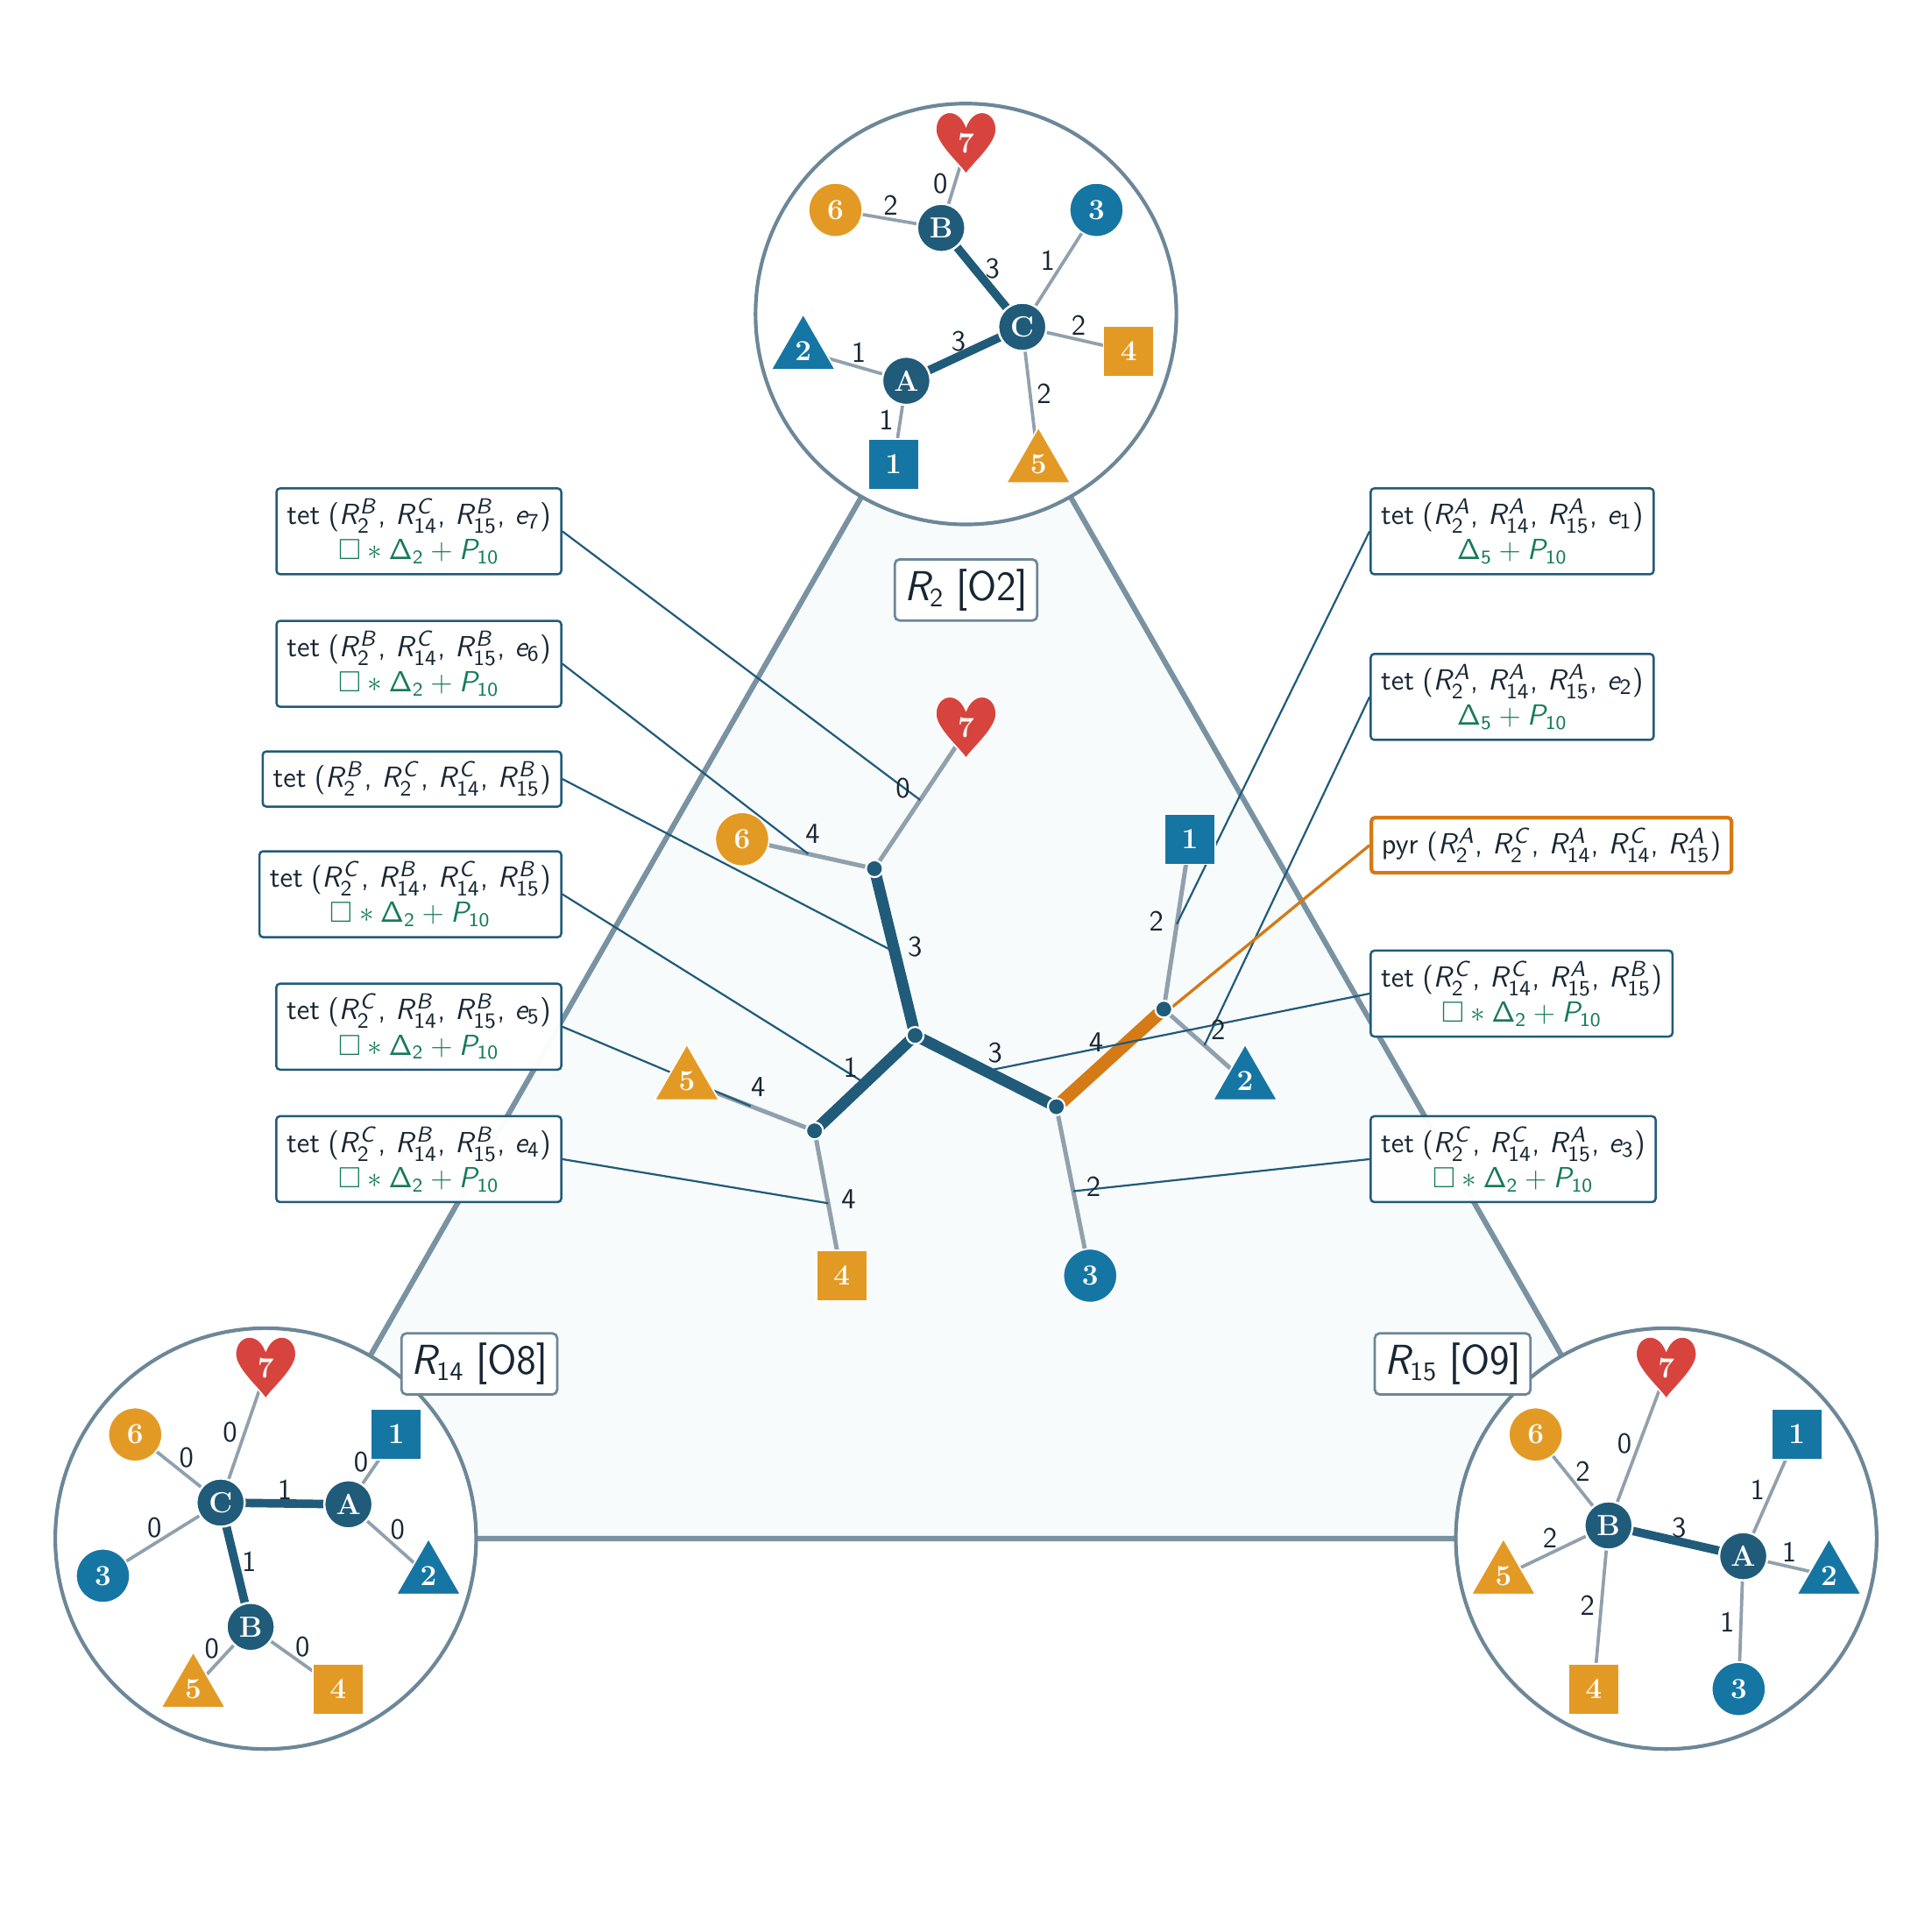
\begin{tikzpicture}[x=1cm,y=1cm]
\path[use as bounding box] (-13.65,-13.65) rectangle (13.65,13.65);
\path[support cell] (0.00000,9.45000)--(-10.15000,-8.30000)--(10.15000,-8.30000)--cycle;
\path[vertex disc] (0.00000,9.45000) circle[radius=3.05000cm];
\path[vertex disc] (-10.15000,-8.30000) circle[radius=3.05000cm];
\path[vertex disc] (10.15000,-8.30000) circle[radius=3.05000cm];
\coordinate (corner-1-v1) at (-1.05000,7.26966);
\coordinate (corner-1-v2) at (-2.35933,8.91150);
\coordinate (corner-1-v3) at (1.89203,10.95885);
\coordinate (corner-1-v4) at (2.35933,8.91150);
\coordinate (corner-1-v5) at (1.05000,7.26966);
\coordinate (corner-1-v6) at (-1.89203,10.95885);
\coordinate (corner-1-v7) at (0.00000,11.87000);
\coordinate (corner-1-v8) at (-0.86458,8.48167);
\coordinate (corner-1-v9) at (-0.35881,10.69756);
\coordinate (corner-1-v10) at (0.81559,9.26385);
\draw[internal edge] (corner-1-v8)--node[mini length,pos=0.5] {\(3\)}(corner-1-v10);
\draw[internal edge] (corner-1-v9)--node[mini length,pos=0.5] {\(3\)}(corner-1-v10);
\draw[pendant edge] (corner-1-v1)--node[mini length,pos=0.5] {\(1\)}(corner-1-v8);
\draw[pendant edge] (corner-1-v2)--node[mini length,pos=0.5] {\(1\)}(corner-1-v8);
\draw[pendant edge] (corner-1-v3)--node[mini length,pos=0.5] {\(1\)}(corner-1-v10);
\draw[pendant edge] (corner-1-v4)--node[mini length,pos=0.5] {\(2\)}(corner-1-v10);
\draw[pendant edge] (corner-1-v5)--node[mini length,pos=0.5] {\(2\)}(corner-1-v10);
\draw[pendant edge] (corner-1-v6)--node[mini length,pos=0.5] {\(2\)}(corner-1-v9);
\draw[pendant edge] (corner-1-v7)--node[mini length,pos=0.5] {\(0\)}(corner-1-v9);
\node[lettered vertex] at (corner-1-v8) {A};
\node[lettered vertex] at (corner-1-v9) {B};
\node[lettered vertex] at (corner-1-v10) {C};
\taxonone{corner-1-v1}
\taxontwo{corner-1-v2}
\taxonthree{corner-1-v3}
\taxonfour{corner-1-v4}
\taxonfive{corner-1-v5}
\taxonsix{corner-1-v6}
\taxonseven{corner-1-v7}
\node[ray title] at (0.00000,5.45000) {\(R_{2}\;[\mathrm{O}2]\)};
\coordinate (corner-2-v1) at (-8.25797,-6.79115);
\coordinate (corner-2-v2) at (-7.79067,-8.83850);
\coordinate (corner-2-v3) at (-12.50933,-8.83850);
\coordinate (corner-2-v4) at (-9.10000,-10.48034);
\coordinate (corner-2-v5) at (-11.20000,-10.48034);
\coordinate (corner-2-v6) at (-12.04203,-6.79115);
\coordinate (corner-2-v7) at (-10.15000,-5.88000);
\coordinate (corner-2-v8) at (-8.95090,-7.80269);
\coordinate (corner-2-v9) at (-10.36802,-9.57970);
\coordinate (corner-2-v10) at (-10.80406,-7.77841);
\draw[internal edge] (corner-2-v8)--node[mini length,pos=0.5] {\(1\)}(corner-2-v10);
\draw[internal edge] (corner-2-v9)--node[mini length,pos=0.5] {\(1\)}(corner-2-v10);
\draw[pendant edge] (corner-2-v1)--node[mini length,pos=0.5] {\(0\)}(corner-2-v8);
\draw[pendant edge] (corner-2-v2)--node[mini length,pos=0.5] {\(0\)}(corner-2-v8);
\draw[pendant edge] (corner-2-v3)--node[mini length,pos=0.5] {\(0\)}(corner-2-v10);
\draw[pendant edge] (corner-2-v4)--node[mini length,pos=0.5] {\(0\)}(corner-2-v9);
\draw[pendant edge] (corner-2-v5)--node[mini length,pos=0.5] {\(0\)}(corner-2-v9);
\draw[pendant edge] (corner-2-v6)--node[mini length,pos=0.5] {\(0\)}(corner-2-v10);
\draw[pendant edge] (corner-2-v7)--node[mini length,pos=0.5] {\(0\)}(corner-2-v10);
\node[lettered vertex] at (corner-2-v8) {A};
\node[lettered vertex] at (corner-2-v9) {B};
\node[lettered vertex] at (corner-2-v10) {C};
\taxonone{corner-2-v1}
\taxontwo{corner-2-v2}
\taxonthree{corner-2-v3}
\taxonfour{corner-2-v4}
\taxonfive{corner-2-v5}
\taxonsix{corner-2-v6}
\taxonseven{corner-2-v7}
\node[ray title] at (-7.05349,-5.76788) {\(R_{14}\;[\mathrm{O}8]\)};
\coordinate (corner-3-v1) at (12.04203,-6.79115);
\coordinate (corner-3-v2) at (12.50933,-8.83850);
\coordinate (corner-3-v3) at (11.20000,-10.48034);
\coordinate (corner-3-v4) at (9.10000,-10.48034);
\coordinate (corner-3-v5) at (7.79067,-8.83850);
\coordinate (corner-3-v6) at (8.25797,-6.79115);
\coordinate (corner-3-v7) at (10.15000,-5.88000);
\coordinate (corner-3-v8) at (11.26608,-8.55474);
\coordinate (corner-3-v9) at (9.31294,-8.10895);
\draw[internal edge] (corner-3-v8)--node[mini length,pos=0.5] {\(3\)}(corner-3-v9);
\draw[pendant edge] (corner-3-v1)--node[mini length,pos=0.5] {\(1\)}(corner-3-v8);
\draw[pendant edge] (corner-3-v2)--node[mini length,pos=0.5] {\(1\)}(corner-3-v8);
\draw[pendant edge] (corner-3-v3)--node[mini length,pos=0.5] {\(1\)}(corner-3-v8);
\draw[pendant edge] (corner-3-v4)--node[mini length,pos=0.5] {\(2\)}(corner-3-v9);
\draw[pendant edge] (corner-3-v5)--node[mini length,pos=0.5] {\(2\)}(corner-3-v9);
\draw[pendant edge] (corner-3-v6)--node[mini length,pos=0.5] {\(2\)}(corner-3-v9);
\draw[pendant edge] (corner-3-v7)--node[mini length,pos=0.5] {\(0\)}(corner-3-v9);
\node[lettered vertex] at (corner-3-v8) {A};
\node[lettered vertex] at (corner-3-v9) {B};
\taxonone{corner-3-v1}
\taxontwo{corner-3-v2}
\taxonthree{corner-3-v3}
\taxonfour{corner-3-v4}
\taxonfive{corner-3-v5}
\taxonsix{corner-3-v6}
\taxonseven{corner-3-v7}
\node[ray title] at (7.05349,-5.76788) {\(R_{15}\;[\mathrm{O}9]\)};
\coordinate (central-v1) at (3.24460,1.83748);
\coordinate (central-v2) at (4.04595,-1.67346);
\coordinate (central-v3) at (1.80062,-4.48902);
\coordinate (central-v4) at (-1.80062,-4.48902);
\coordinate (central-v5) at (-4.04595,-1.67346);
\coordinate (central-v6) at (-3.24460,1.83748);
\coordinate (central-v7) at (0.00000,3.40000);
\coordinate (central-v8) at (2.86687,-0.62544);
\coordinate (central-v9) at (1.31007,-2.04035);
\coordinate (central-v10) at (-1.32729,1.41030);
\coordinate (central-v11) at (-2.19462,-2.38969);
\coordinate (central-v12) at (-0.73728,-1.00658);
\draw[central pyramid edge] (central-v8)--(central-v9);
\draw[central internal edge] (central-v9)--(central-v12);
\draw[central internal edge] (central-v10)--(central-v12);
\draw[central internal edge] (central-v11)--(central-v12);
\draw[central pendant edge] (central-v1)--(central-v8);
\draw[central pendant edge] (central-v2)--(central-v8);
\draw[central pendant edge] (central-v3)--(central-v9);
\draw[central pendant edge] (central-v4)--(central-v11);
\draw[central pendant edge] (central-v5)--(central-v11);
\draw[central pendant edge] (central-v6)--(central-v10);
\draw[central pendant edge] (central-v7)--(central-v10);
\draw[edge leader] (-5.85000,6.30000)--(-0.66365,2.40515);
\draw[edge leader] (-5.85000,4.38000)--(-2.28595,1.62389);
\draw[edge leader] (-5.85000,2.71000)--(-1.03229,0.20186);
\draw[edge leader] (-5.85000,1.04000)--(-1.46595,-1.69813);
\draw[edge leader] (-5.85000,-0.88000)--(-3.12028,-2.03157);
\draw[edge leader] (-5.85000,-2.80000)--(-1.99762,-3.43935);
\draw[edge leader] (5.85000,6.30000)--(3.05574,0.60602);
\draw[edge leader] (5.85000,3.90000)--(3.45641,-1.14945);
\draw[pyramid leader] (5.85000,1.75000)--(2.08847,-1.33289);
\draw[edge leader] (5.85000,-0.40000)--(0.28640,-1.52346);
\draw[edge leader] (5.85000,-2.80000)--(1.55534,-3.26468);
\node[internal vertex] at (central-v8) {};
\node[internal vertex] at (central-v9) {};
\node[internal vertex] at (central-v10) {};
\node[internal vertex] at (central-v11) {};
\node[internal vertex] at (central-v12) {};
\taxonone{central-v1}
\taxontwo{central-v2}
\taxonthree{central-v3}
\taxonfour{central-v4}
\taxonfive{central-v5}
\taxonsix{central-v6}
\taxonseven{central-v7}
\path (central-v8)--node[central length,pos=.50] {\(4\)}(central-v9);
\path (central-v9)--node[central length,pos=.50] {\(3\)}(central-v12);
\path (central-v10)--node[central length,pos=.50] {\(3\)}(central-v12);
\path (central-v11)--node[central length,pos=.50] {\(1\)}(central-v12);
\path (central-v1)--node[central length,pos=.50] {\(2\)}(central-v8);
\path (central-v2)--node[central length,pos=.50] {\(2\)}(central-v8);
\path (central-v3)--node[central length,pos=.50] {\(2\)}(central-v9);
\path (central-v4)--node[central length,pos=.50] {\(4\)}(central-v11);
\path (central-v5)--node[central length,pos=.50] {\(4\)}(central-v11);
\path (central-v6)--node[central length,pos=.50] {\(4\)}(central-v10);
\path (central-v7)--node[central length,pos=.50] {\(0\)}(central-v10);
\node[edge callout,anchor=east] (callout-1) at (-5.85000,6.30000) {\(\mathrm{tet}\;(R_{2}^{B},\,R_{14}^{C},\,R_{15}^{B},\,e_{7})\)\\{\fontsize{12}{14}\selectfont\color{toricgreen}\(\square\ast\Delta_{2}+P_{10}\)}};
\node[edge callout,anchor=east] (callout-2) at (-5.85000,4.38000) {\(\mathrm{tet}\;(R_{2}^{B},\,R_{14}^{C},\,R_{15}^{B},\,e_{6})\)\\{\fontsize{12}{14}\selectfont\color{toricgreen}\(\square\ast\Delta_{2}+P_{10}\)}};
\node[edge callout,anchor=east] (callout-3) at (-5.85000,2.71000) {\(\mathrm{tet}\;(R_{2}^{B},\,R_{2}^{C},\,R_{14}^{C},\,R_{15}^{B})\)};
\node[edge callout,anchor=east] (callout-4) at (-5.85000,1.04000) {\(\mathrm{tet}\;(R_{2}^{C},\,R_{14}^{B},\,R_{14}^{C},\,R_{15}^{B})\)\\{\fontsize{12}{14}\selectfont\color{toricgreen}\(\square\ast\Delta_{2}+P_{10}\)}};
\node[edge callout,anchor=east] (callout-5) at (-5.85000,-0.88000) {\(\mathrm{tet}\;(R_{2}^{C},\,R_{14}^{B},\,R_{15}^{B},\,e_{5})\)\\{\fontsize{12}{14}\selectfont\color{toricgreen}\(\square\ast\Delta_{2}+P_{10}\)}};
\node[edge callout,anchor=east] (callout-6) at (-5.85000,-2.80000) {\(\mathrm{tet}\;(R_{2}^{C},\,R_{14}^{B},\,R_{15}^{B},\,e_{4})\)\\{\fontsize{12}{14}\selectfont\color{toricgreen}\(\square\ast\Delta_{2}+P_{10}\)}};
\node[edge callout,anchor=west] (callout-7) at (5.85000,6.30000) {\(\mathrm{tet}\;(R_{2}^{A},\,R_{14}^{A},\,R_{15}^{A},\,e_{1})\)\\{\fontsize{12}{14}\selectfont\color{toricgreen}\(\Delta_{5}+P_{10}\)}};
\node[edge callout,anchor=west] (callout-8) at (5.85000,3.90000) {\(\mathrm{tet}\;(R_{2}^{A},\,R_{14}^{A},\,R_{15}^{A},\,e_{2})\)\\{\fontsize{12}{14}\selectfont\color{toricgreen}\(\Delta_{5}+P_{10}\)}};
\node[pyramid callout,anchor=west] (callout-9) at (5.85000,1.75000) {\(\mathrm{pyr}\;(R_{2}^{A},\,R_{2}^{C},\,R_{14}^{A},\,R_{14}^{C},\,R_{15}^{A})\)};
\node[edge callout,anchor=west] (callout-10) at (5.85000,-0.40000) {\(\mathrm{tet}\;(R_{2}^{C},\,R_{14}^{C},\,R_{15}^{A},\,R_{15}^{B})\)\\{\fontsize{12}{14}\selectfont\color{toricgreen}\(\square\ast\Delta_{2}+P_{10}\)}};
\node[edge callout,anchor=west] (callout-11) at (5.85000,-2.80000) {\(\mathrm{tet}\;(R_{2}^{C},\,R_{14}^{C},\,R_{15}^{A},\,e_{3})\)\\{\fontsize{12}{14}\selectfont\color{toricgreen}\(\square\ast\Delta_{2}+P_{10}\)}};
\end{tikzpicture}\end{center}\vspace{-1mm}
\begin{atlasbox}\begin{atlaspanel}
\textcolor{toricgreen}{\bfseries PRIME TORIC}\quad \(P_{10}\):\enspace \(\mathrm{Wed}(\mathrm{M}(3,5);\,\Delta_1)\ast\Delta_{0}\)\quad \(f=(11,33,44,29,9)\)\quad 14 lattice points
\end{atlaspanel}\end{atlasbox}
\clearpage
\begin{atlaspanel}[top=1mm,bottom=2mm]
\AtlasSupportOrbitSplit{%
\vspace*{-3mm}\mbox{{\LARGE\bfseries Triangle orbit 11}\hspace{3mm}\raisebox{.8mm}[0pt][0pt]{{\fontsize{16}{18}\selectfont\color{muted}size 6}}}%
}{%
\vspace*{-3mm}{\fontsize{13}{16}\selectfont{\color{muted}\(\mathbb{Q}\) and \(\mathbb{F}_2\)}\quad{\color{muted}\(\underline{\{3,\,9,\,21\}}\), \(\{5,\,10,\,22\}\), \(\{14,\,16,\,30\}\), \(\{14,\,27,\,30\}\), \(\{10,\,22,\,46\}\), \(\{9,\,21,\,47\}\)}\rule[-3mm]{0pt}{3mm}}%
}%
\end{atlaspanel}\vspace{2mm}
\begin{center}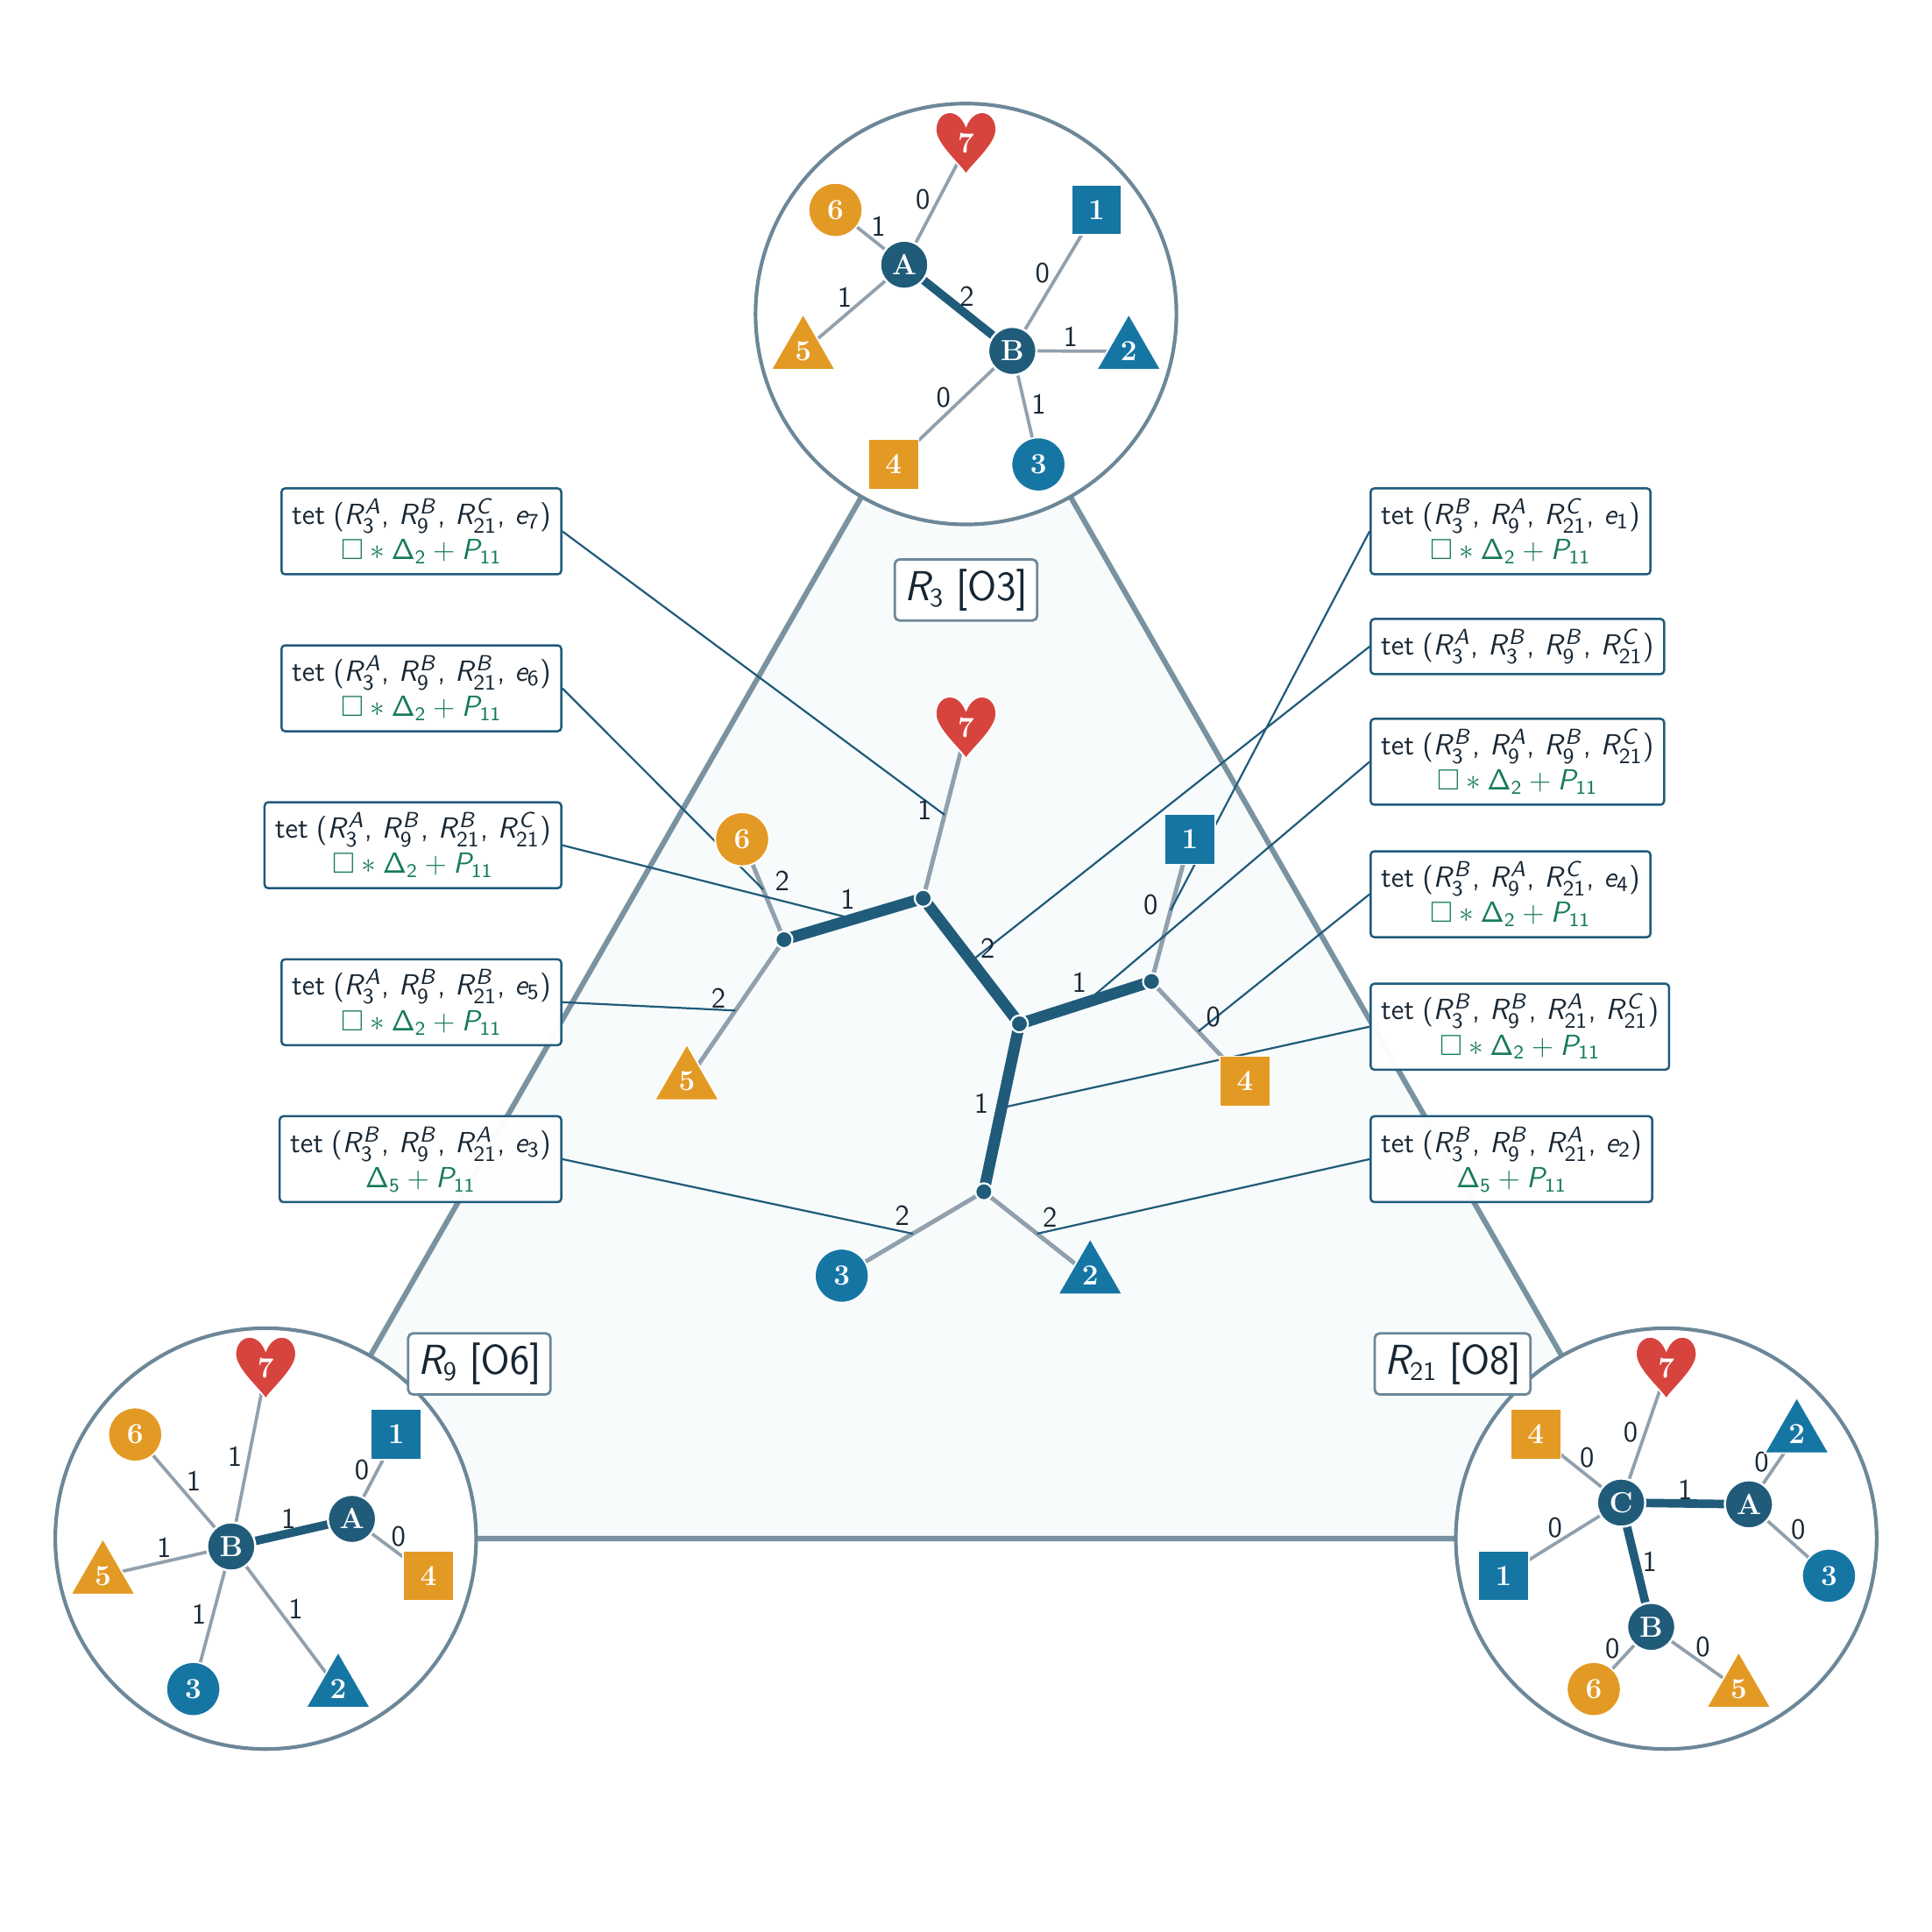
\begin{tikzpicture}[x=1cm,y=1cm]
\path[use as bounding box] (-13.65,-13.65) rectangle (13.65,13.65);
\path[support cell] (0.00000,9.45000)--(-10.15000,-8.30000)--(10.15000,-8.30000)--cycle;
\path[vertex disc] (0.00000,9.45000) circle[radius=3.05000cm];
\path[vertex disc] (-10.15000,-8.30000) circle[radius=3.05000cm];
\path[vertex disc] (10.15000,-8.30000) circle[radius=3.05000cm];
\coordinate (corner-1-v1) at (1.89203,10.95885);
\coordinate (corner-1-v2) at (2.35933,8.91150);
\coordinate (corner-1-v3) at (1.05000,7.26966);
\coordinate (corner-1-v4) at (-1.05000,7.26966);
\coordinate (corner-1-v5) at (-2.35933,8.91150);
\coordinate (corner-1-v6) at (-1.89203,10.95885);
\coordinate (corner-1-v7) at (0.00000,11.87000);
\coordinate (corner-1-v8) at (-0.89502,10.16376);
\coordinate (corner-1-v9) at (0.67127,8.91468);
\draw[internal edge] (corner-1-v8)--node[mini length,pos=0.5] {\(2\)}(corner-1-v9);
\draw[pendant edge] (corner-1-v1)--node[mini length,pos=0.5] {\(0\)}(corner-1-v9);
\draw[pendant edge] (corner-1-v2)--node[mini length,pos=0.5] {\(1\)}(corner-1-v9);
\draw[pendant edge] (corner-1-v3)--node[mini length,pos=0.5] {\(1\)}(corner-1-v9);
\draw[pendant edge] (corner-1-v4)--node[mini length,pos=0.5] {\(0\)}(corner-1-v9);
\draw[pendant edge] (corner-1-v5)--node[mini length,pos=0.5] {\(1\)}(corner-1-v8);
\draw[pendant edge] (corner-1-v6)--node[mini length,pos=0.5] {\(1\)}(corner-1-v8);
\draw[pendant edge] (corner-1-v7)--node[mini length,pos=0.5] {\(0\)}(corner-1-v8);
\node[lettered vertex] at (corner-1-v8) {A};
\node[lettered vertex] at (corner-1-v9) {B};
\taxonone{corner-1-v1}
\taxontwo{corner-1-v2}
\taxonthree{corner-1-v3}
\taxonfour{corner-1-v4}
\taxonfive{corner-1-v5}
\taxonsix{corner-1-v6}
\taxonseven{corner-1-v7}
\node[ray title] at (0.00000,5.45000) {\(R_{3}\;[\mathrm{O}3]\)};
\coordinate (corner-2-v1) at (-8.25797,-6.79115);
\coordinate (corner-2-v2) at (-9.10000,-10.48034);
\coordinate (corner-2-v3) at (-11.20000,-10.48034);
\coordinate (corner-2-v4) at (-7.79067,-8.83850);
\coordinate (corner-2-v5) at (-12.50933,-8.83850);
\coordinate (corner-2-v6) at (-12.04203,-6.79115);
\coordinate (corner-2-v7) at (-10.15000,-5.88000);
\coordinate (corner-2-v8) at (-8.89960,-8.01460);
\coordinate (corner-2-v9) at (-10.65016,-8.41416);
\draw[internal edge] (corner-2-v8)--node[mini length,pos=0.5] {\(1\)}(corner-2-v9);
\draw[pendant edge] (corner-2-v1)--node[mini length,pos=0.5] {\(0\)}(corner-2-v8);
\draw[pendant edge] (corner-2-v2)--node[mini length,pos=0.5] {\(1\)}(corner-2-v9);
\draw[pendant edge] (corner-2-v3)--node[mini length,pos=0.5] {\(1\)}(corner-2-v9);
\draw[pendant edge] (corner-2-v4)--node[mini length,pos=0.5] {\(0\)}(corner-2-v8);
\draw[pendant edge] (corner-2-v5)--node[mini length,pos=0.5] {\(1\)}(corner-2-v9);
\draw[pendant edge] (corner-2-v6)--node[mini length,pos=0.5] {\(1\)}(corner-2-v9);
\draw[pendant edge] (corner-2-v7)--node[mini length,pos=0.5] {\(1\)}(corner-2-v9);
\node[lettered vertex] at (corner-2-v8) {A};
\node[lettered vertex] at (corner-2-v9) {B};
\taxonone{corner-2-v1}
\taxontwo{corner-2-v2}
\taxonthree{corner-2-v3}
\taxonfour{corner-2-v4}
\taxonfive{corner-2-v5}
\taxonsix{corner-2-v6}
\taxonseven{corner-2-v7}
\node[ray title] at (-7.05349,-5.76788) {\(R_{9}\;[\mathrm{O}6]\)};
\coordinate (corner-3-v1) at (7.79067,-8.83850);
\coordinate (corner-3-v2) at (12.04203,-6.79115);
\coordinate (corner-3-v3) at (12.50933,-8.83850);
\coordinate (corner-3-v4) at (8.25797,-6.79115);
\coordinate (corner-3-v5) at (11.20000,-10.48034);
\coordinate (corner-3-v6) at (9.10000,-10.48034);
\coordinate (corner-3-v7) at (10.15000,-5.88000);
\coordinate (corner-3-v8) at (11.34910,-7.80269);
\coordinate (corner-3-v9) at (9.93198,-9.57970);
\coordinate (corner-3-v10) at (9.49594,-7.77841);
\draw[internal edge] (corner-3-v8)--node[mini length,pos=0.5] {\(1\)}(corner-3-v10);
\draw[internal edge] (corner-3-v9)--node[mini length,pos=0.5] {\(1\)}(corner-3-v10);
\draw[pendant edge] (corner-3-v1)--node[mini length,pos=0.5] {\(0\)}(corner-3-v10);
\draw[pendant edge] (corner-3-v2)--node[mini length,pos=0.5] {\(0\)}(corner-3-v8);
\draw[pendant edge] (corner-3-v3)--node[mini length,pos=0.5] {\(0\)}(corner-3-v8);
\draw[pendant edge] (corner-3-v4)--node[mini length,pos=0.5] {\(0\)}(corner-3-v10);
\draw[pendant edge] (corner-3-v5)--node[mini length,pos=0.5] {\(0\)}(corner-3-v9);
\draw[pendant edge] (corner-3-v6)--node[mini length,pos=0.5] {\(0\)}(corner-3-v9);
\draw[pendant edge] (corner-3-v7)--node[mini length,pos=0.5] {\(0\)}(corner-3-v10);
\node[lettered vertex] at (corner-3-v8) {A};
\node[lettered vertex] at (corner-3-v9) {B};
\node[lettered vertex] at (corner-3-v10) {C};
\taxonone{corner-3-v1}
\taxontwo{corner-3-v2}
\taxonthree{corner-3-v3}
\taxonfour{corner-3-v4}
\taxonfive{corner-3-v5}
\taxonsix{corner-3-v6}
\taxonseven{corner-3-v7}
\node[ray title] at (7.05349,-5.76788) {\(R_{21}\;[\mathrm{O}8]\)};
\coordinate (central-v1) at (3.24460,1.83748);
\coordinate (central-v2) at (1.80062,-4.48902);
\coordinate (central-v3) at (-1.80062,-4.48902);
\coordinate (central-v4) at (4.04595,-1.67346);
\coordinate (central-v5) at (-4.04595,-1.67346);
\coordinate (central-v6) at (-3.24460,1.83748);
\coordinate (central-v7) at (0.00000,3.40000);
\coordinate (central-v8) at (-2.63701,0.38167);
\coordinate (central-v9) at (-0.62047,0.98098);
\coordinate (central-v10) at (2.68871,-0.22490);
\coordinate (central-v11) at (0.25853,-3.27226);
\coordinate (central-v12) at (0.77559,-0.83873);
\draw[central internal edge] (central-v8)--(central-v9);
\draw[central internal edge] (central-v9)--(central-v12);
\draw[central internal edge] (central-v10)--(central-v12);
\draw[central internal edge] (central-v11)--(central-v12);
\draw[central pendant edge] (central-v1)--(central-v10);
\draw[central pendant edge] (central-v2)--(central-v11);
\draw[central pendant edge] (central-v3)--(central-v11);
\draw[central pendant edge] (central-v4)--(central-v10);
\draw[central pendant edge] (central-v5)--(central-v8);
\draw[central pendant edge] (central-v6)--(central-v8);
\draw[central pendant edge] (central-v7)--(central-v9);
\draw[edge leader] (-5.85000,6.30000)--(-0.31024,2.19049);
\draw[edge leader] (-5.85000,4.02500)--(-2.94080,1.10957);
\draw[edge leader] (-5.85000,1.75000)--(-1.62874,0.68132);
\draw[edge leader] (-5.85000,-0.52500)--(-3.34148,-0.64590);
\draw[edge leader] (-5.85000,-2.80000)--(-0.77104,-3.88064);
\draw[edge leader] (5.85000,6.30000)--(2.96666,0.80629);
\draw[edge leader] (5.85000,4.63000)--(0.07756,0.07113);
\draw[edge leader] (5.85000,2.96000)--(1.73215,-0.53181);
\draw[edge leader] (5.85000,1.04000)--(3.36733,-0.94918);
\draw[edge leader] (5.85000,-0.88000)--(0.51706,-2.05549);
\draw[edge leader] (5.85000,-2.80000)--(1.02957,-3.88064);
\node[internal vertex] at (central-v8) {};
\node[internal vertex] at (central-v9) {};
\node[internal vertex] at (central-v10) {};
\node[internal vertex] at (central-v11) {};
\node[internal vertex] at (central-v12) {};
\taxonone{central-v1}
\taxontwo{central-v2}
\taxonthree{central-v3}
\taxonfour{central-v4}
\taxonfive{central-v5}
\taxonsix{central-v6}
\taxonseven{central-v7}
\path (central-v8)--node[central length,pos=.50] {\(1\)}(central-v9);
\path (central-v9)--node[central length,pos=.50] {\(2\)}(central-v12);
\path (central-v10)--node[central length,pos=.50] {\(1\)}(central-v12);
\path (central-v11)--node[central length,pos=.50] {\(1\)}(central-v12);
\path (central-v1)--node[central length,pos=.50] {\(0\)}(central-v10);
\path (central-v2)--node[central length,pos=.50] {\(2\)}(central-v11);
\path (central-v3)--node[central length,pos=.50] {\(2\)}(central-v11);
\path (central-v4)--node[central length,pos=.50] {\(0\)}(central-v10);
\path (central-v5)--node[central length,pos=.50] {\(2\)}(central-v8);
\path (central-v6)--node[central length,pos=.50] {\(2\)}(central-v8);
\path (central-v7)--node[central length,pos=.50] {\(1\)}(central-v9);
\node[edge callout,anchor=east] (callout-1) at (-5.85000,6.30000) {\(\mathrm{tet}\;(R_{3}^{A},\,R_{9}^{B},\,R_{21}^{C},\,e_{7})\)\\{\fontsize{12}{14}\selectfont\color{toricgreen}\(\square\ast\Delta_{2}+P_{11}\)}};
\node[edge callout,anchor=east] (callout-2) at (-5.85000,4.02500) {\(\mathrm{tet}\;(R_{3}^{A},\,R_{9}^{B},\,R_{21}^{B},\,e_{6})\)\\{\fontsize{12}{14}\selectfont\color{toricgreen}\(\square\ast\Delta_{2}+P_{11}\)}};
\node[edge callout,anchor=east] (callout-3) at (-5.85000,1.75000) {\(\mathrm{tet}\;(R_{3}^{A},\,R_{9}^{B},\,R_{21}^{B},\,R_{21}^{C})\)\\{\fontsize{12}{14}\selectfont\color{toricgreen}\(\square\ast\Delta_{2}+P_{11}\)}};
\node[edge callout,anchor=east] (callout-4) at (-5.85000,-0.52500) {\(\mathrm{tet}\;(R_{3}^{A},\,R_{9}^{B},\,R_{21}^{B},\,e_{5})\)\\{\fontsize{12}{14}\selectfont\color{toricgreen}\(\square\ast\Delta_{2}+P_{11}\)}};
\node[edge callout,anchor=east] (callout-5) at (-5.85000,-2.80000) {\(\mathrm{tet}\;(R_{3}^{B},\,R_{9}^{B},\,R_{21}^{A},\,e_{3})\)\\{\fontsize{12}{14}\selectfont\color{toricgreen}\(\Delta_{5}+P_{11}\)}};
\node[edge callout,anchor=west] (callout-6) at (5.85000,6.30000) {\(\mathrm{tet}\;(R_{3}^{B},\,R_{9}^{A},\,R_{21}^{C},\,e_{1})\)\\{\fontsize{12}{14}\selectfont\color{toricgreen}\(\square\ast\Delta_{2}+P_{11}\)}};
\node[edge callout,anchor=west] (callout-7) at (5.85000,4.63000) {\(\mathrm{tet}\;(R_{3}^{A},\,R_{3}^{B},\,R_{9}^{B},\,R_{21}^{C})\)};
\node[edge callout,anchor=west] (callout-8) at (5.85000,2.96000) {\(\mathrm{tet}\;(R_{3}^{B},\,R_{9}^{A},\,R_{9}^{B},\,R_{21}^{C})\)\\{\fontsize{12}{14}\selectfont\color{toricgreen}\(\square\ast\Delta_{2}+P_{11}\)}};
\node[edge callout,anchor=west] (callout-9) at (5.85000,1.04000) {\(\mathrm{tet}\;(R_{3}^{B},\,R_{9}^{A},\,R_{21}^{C},\,e_{4})\)\\{\fontsize{12}{14}\selectfont\color{toricgreen}\(\square\ast\Delta_{2}+P_{11}\)}};
\node[edge callout,anchor=west] (callout-10) at (5.85000,-0.88000) {\(\mathrm{tet}\;(R_{3}^{B},\,R_{9}^{B},\,R_{21}^{A},\,R_{21}^{C})\)\\{\fontsize{12}{14}\selectfont\color{toricgreen}\(\square\ast\Delta_{2}+P_{11}\)}};
\node[edge callout,anchor=west] (callout-11) at (5.85000,-2.80000) {\(\mathrm{tet}\;(R_{3}^{B},\,R_{9}^{B},\,R_{21}^{A},\,e_{2})\)\\{\fontsize{12}{14}\selectfont\color{toricgreen}\(\Delta_{5}+P_{11}\)}};
\end{tikzpicture}\end{center}\vspace{-1mm}
\begin{atlasbox}\begin{atlaspanel}
\textcolor{toricgreen}{\bfseries PRIME TORIC}\quad \(P_{11}\):\enspace \(\mathrm{Wed}(\mathrm{M}(3,5);\,\Delta_1)\ast\Delta_{0}\)\quad \(f=(11,33,44,29,9)\)\quad 14 lattice points
\end{atlaspanel}\end{atlasbox}
\clearpage
\begin{atlaspanel}[top=1mm,bottom=2mm]
\AtlasSupportOrbitSplit{%
\vspace*{-3mm}\mbox{{\LARGE\bfseries Triangle orbit 12}\hspace{3mm}\raisebox{.8mm}[0pt][0pt]{{\fontsize{16}{18}\selectfont\color{muted}size 6}}}%
}{%
\vspace*{-3mm}{\fontsize{13}{16}\selectfont{\color{muted}\(\mathbb{Q}\) and \(\mathbb{F}_2\)}\quad{\color{muted}\(\underline{\{3,\,15,\,21\}}\), \(\{5,\,15,\,22\}\), \(\{14,\,16,\,29\}\), \(\{14,\,15,\,27\}\), \(\{22,\,29,\,46\}\), \(\{21,\,29,\,47\}\)}\rule[-3mm]{0pt}{3mm}}%
}%
\end{atlaspanel}\vspace{2mm}
\begin{center}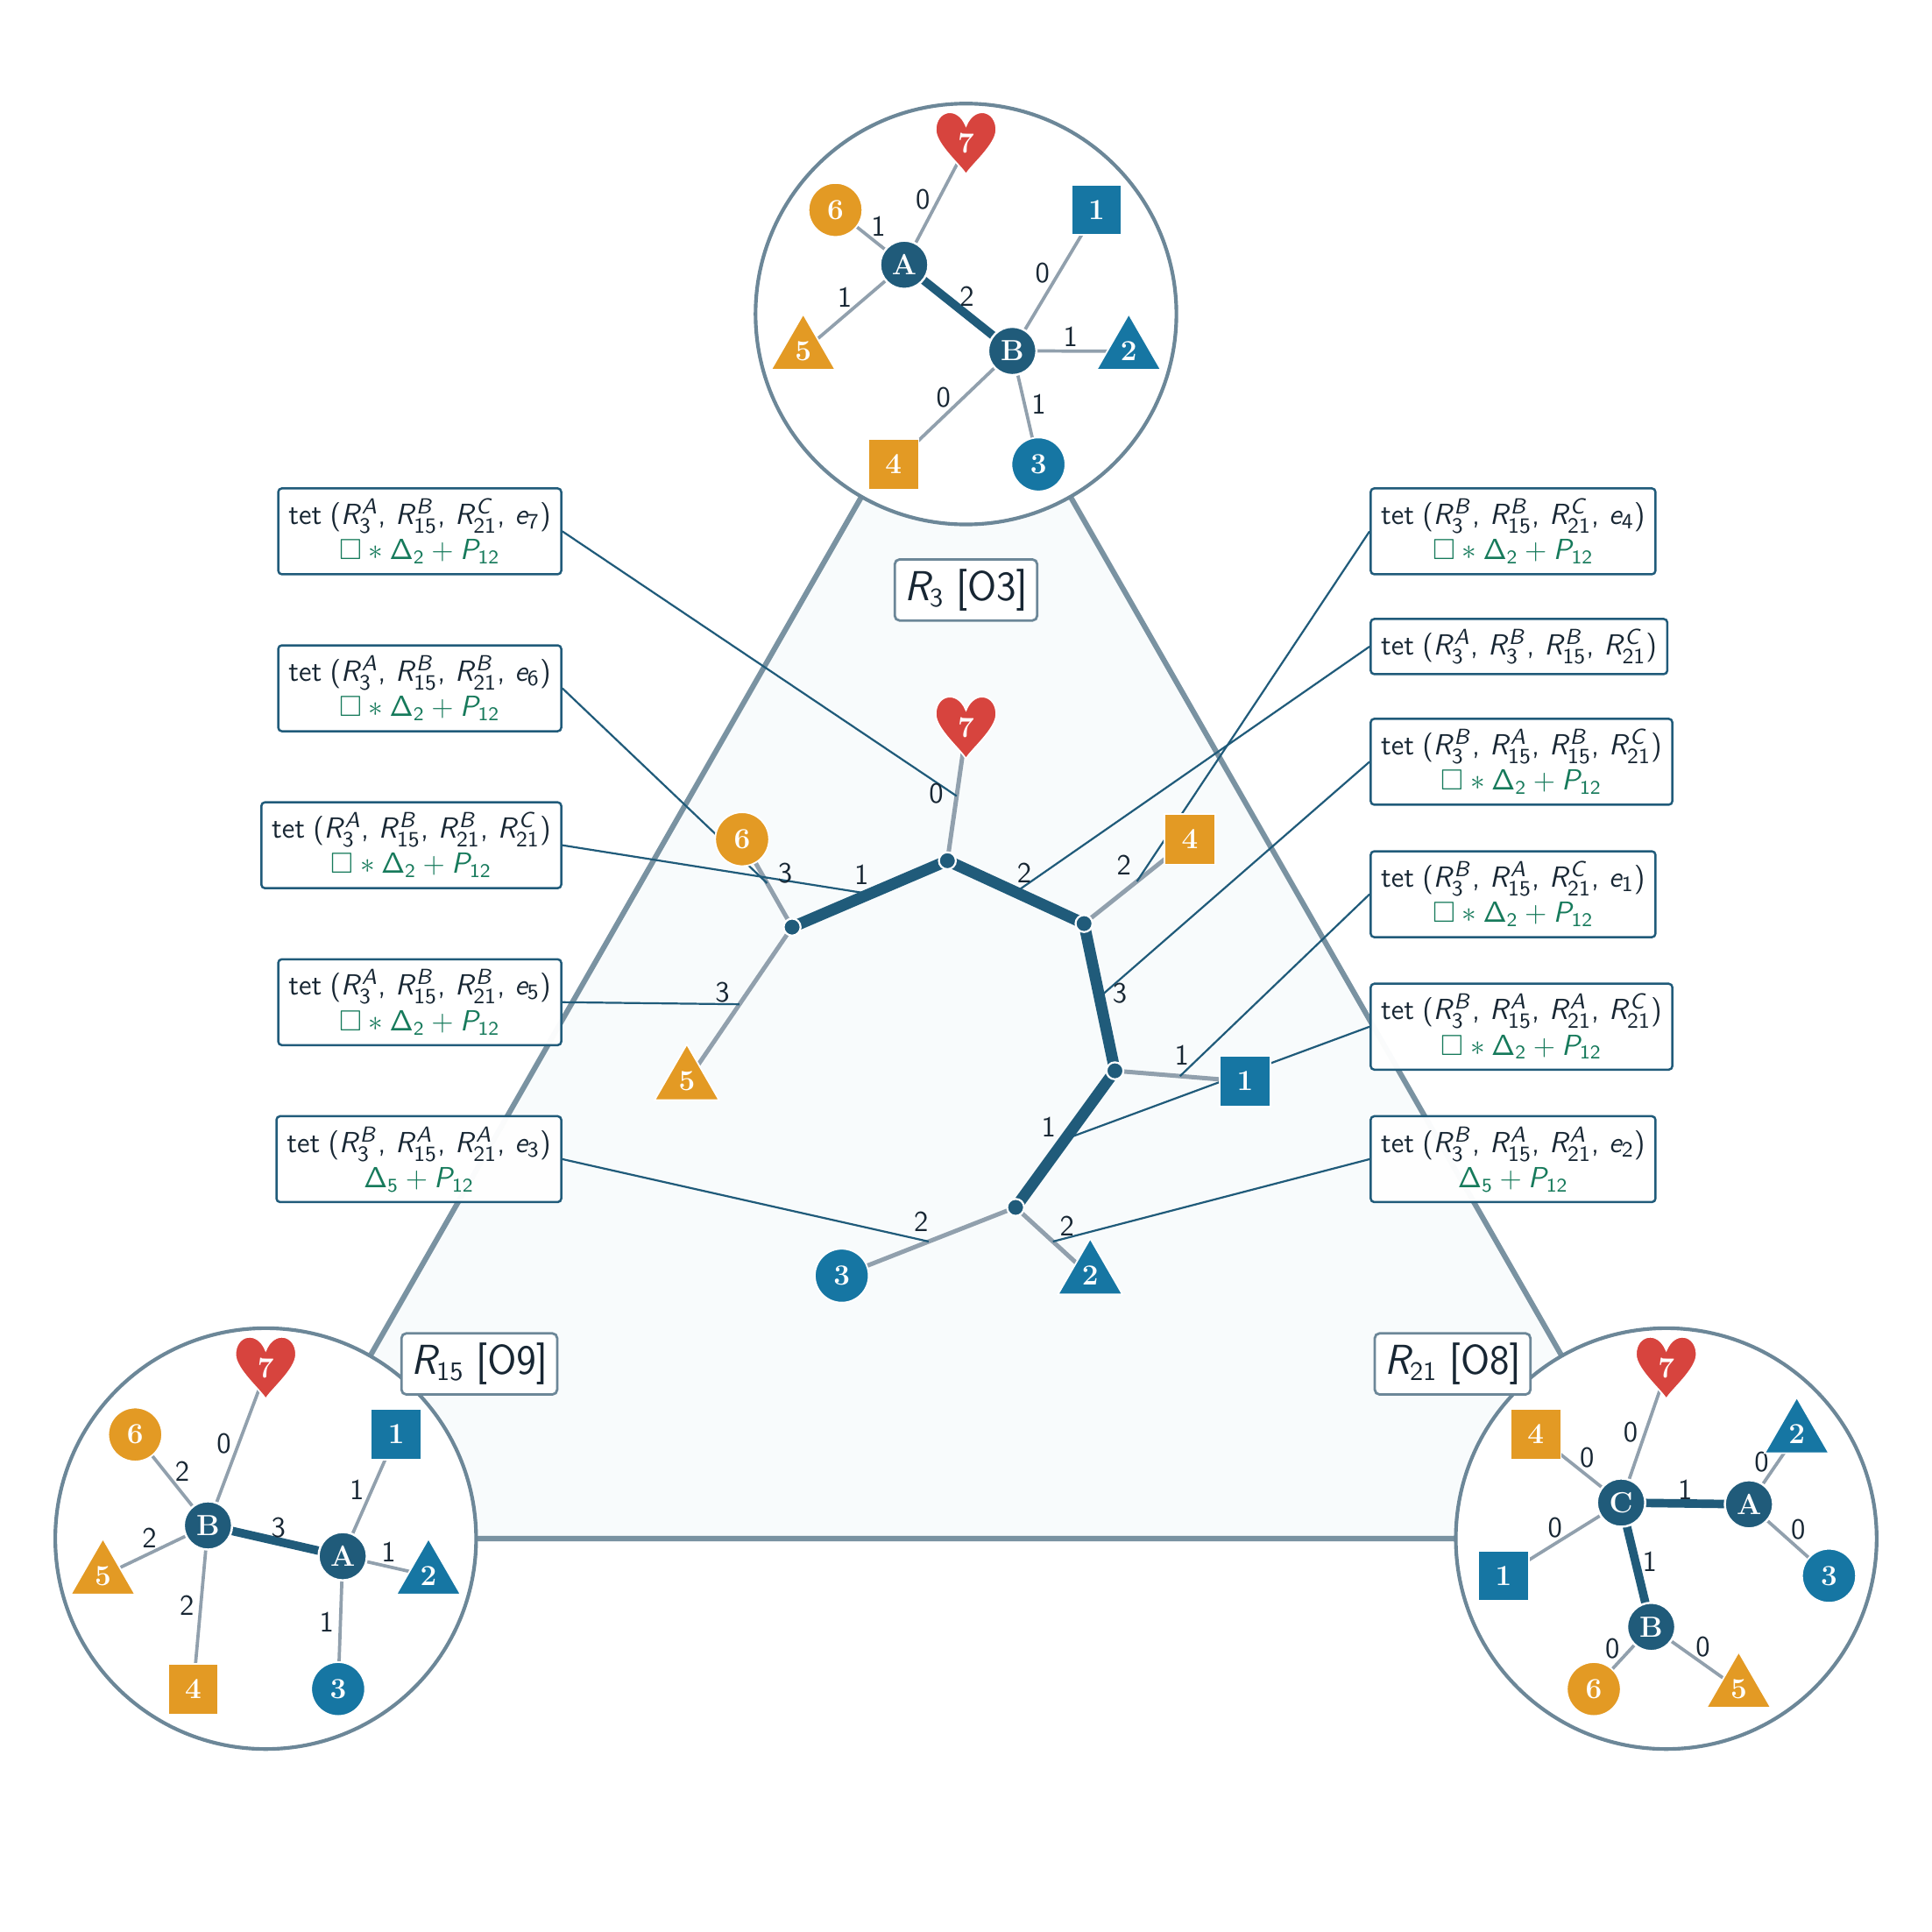
\begin{tikzpicture}[x=1cm,y=1cm]
\path[use as bounding box] (-13.65,-13.65) rectangle (13.65,13.65);
\path[support cell] (0.00000,9.45000)--(-10.15000,-8.30000)--(10.15000,-8.30000)--cycle;
\path[vertex disc] (0.00000,9.45000) circle[radius=3.05000cm];
\path[vertex disc] (-10.15000,-8.30000) circle[radius=3.05000cm];
\path[vertex disc] (10.15000,-8.30000) circle[radius=3.05000cm];
\coordinate (corner-1-v1) at (1.89203,10.95885);
\coordinate (corner-1-v2) at (2.35933,8.91150);
\coordinate (corner-1-v3) at (1.05000,7.26966);
\coordinate (corner-1-v4) at (-1.05000,7.26966);
\coordinate (corner-1-v5) at (-2.35933,8.91150);
\coordinate (corner-1-v6) at (-1.89203,10.95885);
\coordinate (corner-1-v7) at (0.00000,11.87000);
\coordinate (corner-1-v8) at (-0.89502,10.16376);
\coordinate (corner-1-v9) at (0.67127,8.91468);
\draw[internal edge] (corner-1-v8)--node[mini length,pos=0.5] {\(2\)}(corner-1-v9);
\draw[pendant edge] (corner-1-v1)--node[mini length,pos=0.5] {\(0\)}(corner-1-v9);
\draw[pendant edge] (corner-1-v2)--node[mini length,pos=0.5] {\(1\)}(corner-1-v9);
\draw[pendant edge] (corner-1-v3)--node[mini length,pos=0.5] {\(1\)}(corner-1-v9);
\draw[pendant edge] (corner-1-v4)--node[mini length,pos=0.5] {\(0\)}(corner-1-v9);
\draw[pendant edge] (corner-1-v5)--node[mini length,pos=0.5] {\(1\)}(corner-1-v8);
\draw[pendant edge] (corner-1-v6)--node[mini length,pos=0.5] {\(1\)}(corner-1-v8);
\draw[pendant edge] (corner-1-v7)--node[mini length,pos=0.5] {\(0\)}(corner-1-v8);
\node[lettered vertex] at (corner-1-v8) {A};
\node[lettered vertex] at (corner-1-v9) {B};
\taxonone{corner-1-v1}
\taxontwo{corner-1-v2}
\taxonthree{corner-1-v3}
\taxonfour{corner-1-v4}
\taxonfive{corner-1-v5}
\taxonsix{corner-1-v6}
\taxonseven{corner-1-v7}
\node[ray title] at (0.00000,5.45000) {\(R_{3}\;[\mathrm{O}3]\)};
\coordinate (corner-2-v1) at (-8.25797,-6.79115);
\coordinate (corner-2-v2) at (-7.79067,-8.83850);
\coordinate (corner-2-v3) at (-9.10000,-10.48034);
\coordinate (corner-2-v4) at (-11.20000,-10.48034);
\coordinate (corner-2-v5) at (-12.50933,-8.83850);
\coordinate (corner-2-v6) at (-12.04203,-6.79115);
\coordinate (corner-2-v7) at (-10.15000,-5.88000);
\coordinate (corner-2-v8) at (-9.03392,-8.55474);
\coordinate (corner-2-v9) at (-10.98706,-8.10895);
\draw[internal edge] (corner-2-v8)--node[mini length,pos=0.5] {\(3\)}(corner-2-v9);
\draw[pendant edge] (corner-2-v1)--node[mini length,pos=0.5] {\(1\)}(corner-2-v8);
\draw[pendant edge] (corner-2-v2)--node[mini length,pos=0.5] {\(1\)}(corner-2-v8);
\draw[pendant edge] (corner-2-v3)--node[mini length,pos=0.5] {\(1\)}(corner-2-v8);
\draw[pendant edge] (corner-2-v4)--node[mini length,pos=0.5] {\(2\)}(corner-2-v9);
\draw[pendant edge] (corner-2-v5)--node[mini length,pos=0.5] {\(2\)}(corner-2-v9);
\draw[pendant edge] (corner-2-v6)--node[mini length,pos=0.5] {\(2\)}(corner-2-v9);
\draw[pendant edge] (corner-2-v7)--node[mini length,pos=0.5] {\(0\)}(corner-2-v9);
\node[lettered vertex] at (corner-2-v8) {A};
\node[lettered vertex] at (corner-2-v9) {B};
\taxonone{corner-2-v1}
\taxontwo{corner-2-v2}
\taxonthree{corner-2-v3}
\taxonfour{corner-2-v4}
\taxonfive{corner-2-v5}
\taxonsix{corner-2-v6}
\taxonseven{corner-2-v7}
\node[ray title] at (-7.05349,-5.76788) {\(R_{15}\;[\mathrm{O}9]\)};
\coordinate (corner-3-v1) at (7.79067,-8.83850);
\coordinate (corner-3-v2) at (12.04203,-6.79115);
\coordinate (corner-3-v3) at (12.50933,-8.83850);
\coordinate (corner-3-v4) at (8.25797,-6.79115);
\coordinate (corner-3-v5) at (11.20000,-10.48034);
\coordinate (corner-3-v6) at (9.10000,-10.48034);
\coordinate (corner-3-v7) at (10.15000,-5.88000);
\coordinate (corner-3-v8) at (11.34910,-7.80269);
\coordinate (corner-3-v9) at (9.93198,-9.57970);
\coordinate (corner-3-v10) at (9.49594,-7.77841);
\draw[internal edge] (corner-3-v8)--node[mini length,pos=0.5] {\(1\)}(corner-3-v10);
\draw[internal edge] (corner-3-v9)--node[mini length,pos=0.5] {\(1\)}(corner-3-v10);
\draw[pendant edge] (corner-3-v1)--node[mini length,pos=0.5] {\(0\)}(corner-3-v10);
\draw[pendant edge] (corner-3-v2)--node[mini length,pos=0.5] {\(0\)}(corner-3-v8);
\draw[pendant edge] (corner-3-v3)--node[mini length,pos=0.5] {\(0\)}(corner-3-v8);
\draw[pendant edge] (corner-3-v4)--node[mini length,pos=0.5] {\(0\)}(corner-3-v10);
\draw[pendant edge] (corner-3-v5)--node[mini length,pos=0.5] {\(0\)}(corner-3-v9);
\draw[pendant edge] (corner-3-v6)--node[mini length,pos=0.5] {\(0\)}(corner-3-v9);
\draw[pendant edge] (corner-3-v7)--node[mini length,pos=0.5] {\(0\)}(corner-3-v10);
\node[lettered vertex] at (corner-3-v8) {A};
\node[lettered vertex] at (corner-3-v9) {B};
\node[lettered vertex] at (corner-3-v10) {C};
\taxonone{corner-3-v1}
\taxontwo{corner-3-v2}
\taxonthree{corner-3-v3}
\taxonfour{corner-3-v4}
\taxonfive{corner-3-v5}
\taxonsix{corner-3-v6}
\taxonseven{corner-3-v7}
\node[ray title] at (7.05349,-5.76788) {\(R_{21}\;[\mathrm{O}8]\)};
\coordinate (central-v1) at (4.04595,-1.67346);
\coordinate (central-v2) at (1.80062,-4.48902);
\coordinate (central-v3) at (-1.80062,-4.48902);
\coordinate (central-v4) at (3.24460,1.83748);
\coordinate (central-v5) at (-4.04595,-1.67346);
\coordinate (central-v6) at (-3.24460,1.83748);
\coordinate (central-v7) at (0.00000,3.40000);
\coordinate (central-v8) at (0.71966,-3.49910);
\coordinate (central-v9) at (2.15898,-1.51927);
\coordinate (central-v10) at (1.71134,0.61475);
\coordinate (central-v11) at (-2.52004,0.56335);
\coordinate (central-v12) at (-0.26957,1.52603);
\draw[central internal edge] (central-v8)--(central-v9);
\draw[central internal edge] (central-v9)--(central-v10);
\draw[central internal edge] (central-v10)--(central-v12);
\draw[central internal edge] (central-v11)--(central-v12);
\draw[central pendant edge] (central-v1)--(central-v9);
\draw[central pendant edge] (central-v2)--(central-v8);
\draw[central pendant edge] (central-v3)--(central-v8);
\draw[central pendant edge] (central-v4)--(central-v10);
\draw[central pendant edge] (central-v5)--(central-v11);
\draw[central pendant edge] (central-v6)--(central-v11);
\draw[central pendant edge] (central-v7)--(central-v12);
\draw[edge leader] (-5.85000,6.30000)--(-0.13478,2.46302);
\draw[edge leader] (-5.85000,4.02500)--(-2.88232,1.20042);
\draw[edge leader] (-5.85000,1.75000)--(-1.39480,1.04469);
\draw[edge leader] (-5.85000,-0.52500)--(-3.28300,-0.55506);
\draw[edge leader] (-5.85000,-2.80000)--(-0.54048,-3.99406);
\draw[edge leader] (5.85000,6.30000)--(2.47797,1.22612);
\draw[edge leader] (5.85000,4.63000)--(0.72089,1.07039);
\draw[edge leader] (5.85000,2.96000)--(1.93516,-0.45226);
\draw[edge leader] (5.85000,1.04000)--(3.10247,-1.59637);
\draw[edge leader] (5.85000,-0.88000)--(1.43932,-2.50919);
\draw[edge leader] (5.85000,-2.80000)--(1.26014,-3.99406);
\node[internal vertex] at (central-v8) {};
\node[internal vertex] at (central-v9) {};
\node[internal vertex] at (central-v10) {};
\node[internal vertex] at (central-v11) {};
\node[internal vertex] at (central-v12) {};
\taxonone{central-v1}
\taxontwo{central-v2}
\taxonthree{central-v3}
\taxonfour{central-v4}
\taxonfive{central-v5}
\taxonsix{central-v6}
\taxonseven{central-v7}
\path (central-v8)--node[central length,pos=.50] {\(1\)}(central-v9);
\path (central-v9)--node[central length,pos=.50] {\(3\)}(central-v10);
\path (central-v10)--node[central length,pos=.50] {\(2\)}(central-v12);
\path (central-v11)--node[central length,pos=.50] {\(1\)}(central-v12);
\path (central-v1)--node[central length,pos=.50] {\(1\)}(central-v9);
\path (central-v2)--node[central length,pos=.50] {\(2\)}(central-v8);
\path (central-v3)--node[central length,pos=.50] {\(2\)}(central-v8);
\path (central-v4)--node[central length,pos=.50] {\(2\)}(central-v10);
\path (central-v5)--node[central length,pos=.50] {\(3\)}(central-v11);
\path (central-v6)--node[central length,pos=.50] {\(3\)}(central-v11);
\path (central-v7)--node[central length,pos=.50] {\(0\)}(central-v12);
\node[edge callout,anchor=east] (callout-1) at (-5.85000,6.30000) {\(\mathrm{tet}\;(R_{3}^{A},\,R_{15}^{B},\,R_{21}^{C},\,e_{7})\)\\{\fontsize{12}{14}\selectfont\color{toricgreen}\(\square\ast\Delta_{2}+P_{12}\)}};
\node[edge callout,anchor=east] (callout-2) at (-5.85000,4.02500) {\(\mathrm{tet}\;(R_{3}^{A},\,R_{15}^{B},\,R_{21}^{B},\,e_{6})\)\\{\fontsize{12}{14}\selectfont\color{toricgreen}\(\square\ast\Delta_{2}+P_{12}\)}};
\node[edge callout,anchor=east] (callout-3) at (-5.85000,1.75000) {\(\mathrm{tet}\;(R_{3}^{A},\,R_{15}^{B},\,R_{21}^{B},\,R_{21}^{C})\)\\{\fontsize{12}{14}\selectfont\color{toricgreen}\(\square\ast\Delta_{2}+P_{12}\)}};
\node[edge callout,anchor=east] (callout-4) at (-5.85000,-0.52500) {\(\mathrm{tet}\;(R_{3}^{A},\,R_{15}^{B},\,R_{21}^{B},\,e_{5})\)\\{\fontsize{12}{14}\selectfont\color{toricgreen}\(\square\ast\Delta_{2}+P_{12}\)}};
\node[edge callout,anchor=east] (callout-5) at (-5.85000,-2.80000) {\(\mathrm{tet}\;(R_{3}^{B},\,R_{15}^{A},\,R_{21}^{A},\,e_{3})\)\\{\fontsize{12}{14}\selectfont\color{toricgreen}\(\Delta_{5}+P_{12}\)}};
\node[edge callout,anchor=west] (callout-6) at (5.85000,6.30000) {\(\mathrm{tet}\;(R_{3}^{B},\,R_{15}^{B},\,R_{21}^{C},\,e_{4})\)\\{\fontsize{12}{14}\selectfont\color{toricgreen}\(\square\ast\Delta_{2}+P_{12}\)}};
\node[edge callout,anchor=west] (callout-7) at (5.85000,4.63000) {\(\mathrm{tet}\;(R_{3}^{A},\,R_{3}^{B},\,R_{15}^{B},\,R_{21}^{C})\)};
\node[edge callout,anchor=west] (callout-8) at (5.85000,2.96000) {\(\mathrm{tet}\;(R_{3}^{B},\,R_{15}^{A},\,R_{15}^{B},\,R_{21}^{C})\)\\{\fontsize{12}{14}\selectfont\color{toricgreen}\(\square\ast\Delta_{2}+P_{12}\)}};
\node[edge callout,anchor=west] (callout-9) at (5.85000,1.04000) {\(\mathrm{tet}\;(R_{3}^{B},\,R_{15}^{A},\,R_{21}^{C},\,e_{1})\)\\{\fontsize{12}{14}\selectfont\color{toricgreen}\(\square\ast\Delta_{2}+P_{12}\)}};
\node[edge callout,anchor=west] (callout-10) at (5.85000,-0.88000) {\(\mathrm{tet}\;(R_{3}^{B},\,R_{15}^{A},\,R_{21}^{A},\,R_{21}^{C})\)\\{\fontsize{12}{14}\selectfont\color{toricgreen}\(\square\ast\Delta_{2}+P_{12}\)}};
\node[edge callout,anchor=west] (callout-11) at (5.85000,-2.80000) {\(\mathrm{tet}\;(R_{3}^{B},\,R_{15}^{A},\,R_{21}^{A},\,e_{2})\)\\{\fontsize{12}{14}\selectfont\color{toricgreen}\(\Delta_{5}+P_{12}\)}};
\end{tikzpicture}\end{center}\vspace{-1mm}
\begin{atlasbox}\begin{atlaspanel}
\textcolor{toricgreen}{\bfseries PRIME TORIC}\quad \(P_{12}\):\enspace \(\mathrm{Wed}(\mathrm{M}(3,5)\ast\Delta_{0};\,\Delta_2)\)\quad \(f=(11,33,44,29,9)\)\quad 14 lattice points
\end{atlaspanel}\end{atlasbox}
\clearpage
\begin{atlaspanel}[top=1mm,bottom=2mm]
\AtlasSupportOrbitSplit{%
\vspace*{-3mm}\mbox{{\LARGE\bfseries Triangle orbit 13}\hspace{3mm}\raisebox{.8mm}[0pt][0pt]{{\fontsize{16}{18}\selectfont\color{muted}size 6}}}%
}{%
\vspace*{-3mm}{\fontsize{13}{16}\selectfont{\color{muted}\(\mathbb{Q}\) and \(\mathbb{F}_2\)}\quad{\color{muted}\(\underline{\{8,\,9,\,37\}}\), \(\{8,\,10,\,37\}\), \(\{9,\,33,\,37\}\), \(\{30,\,33,\,37\}\), \(\{10,\,34,\,37\}\), \(\{30,\,34,\,37\}\)}\rule[-3mm]{0pt}{3mm}}%
}%
\end{atlaspanel}\vspace{2mm}
\begin{center}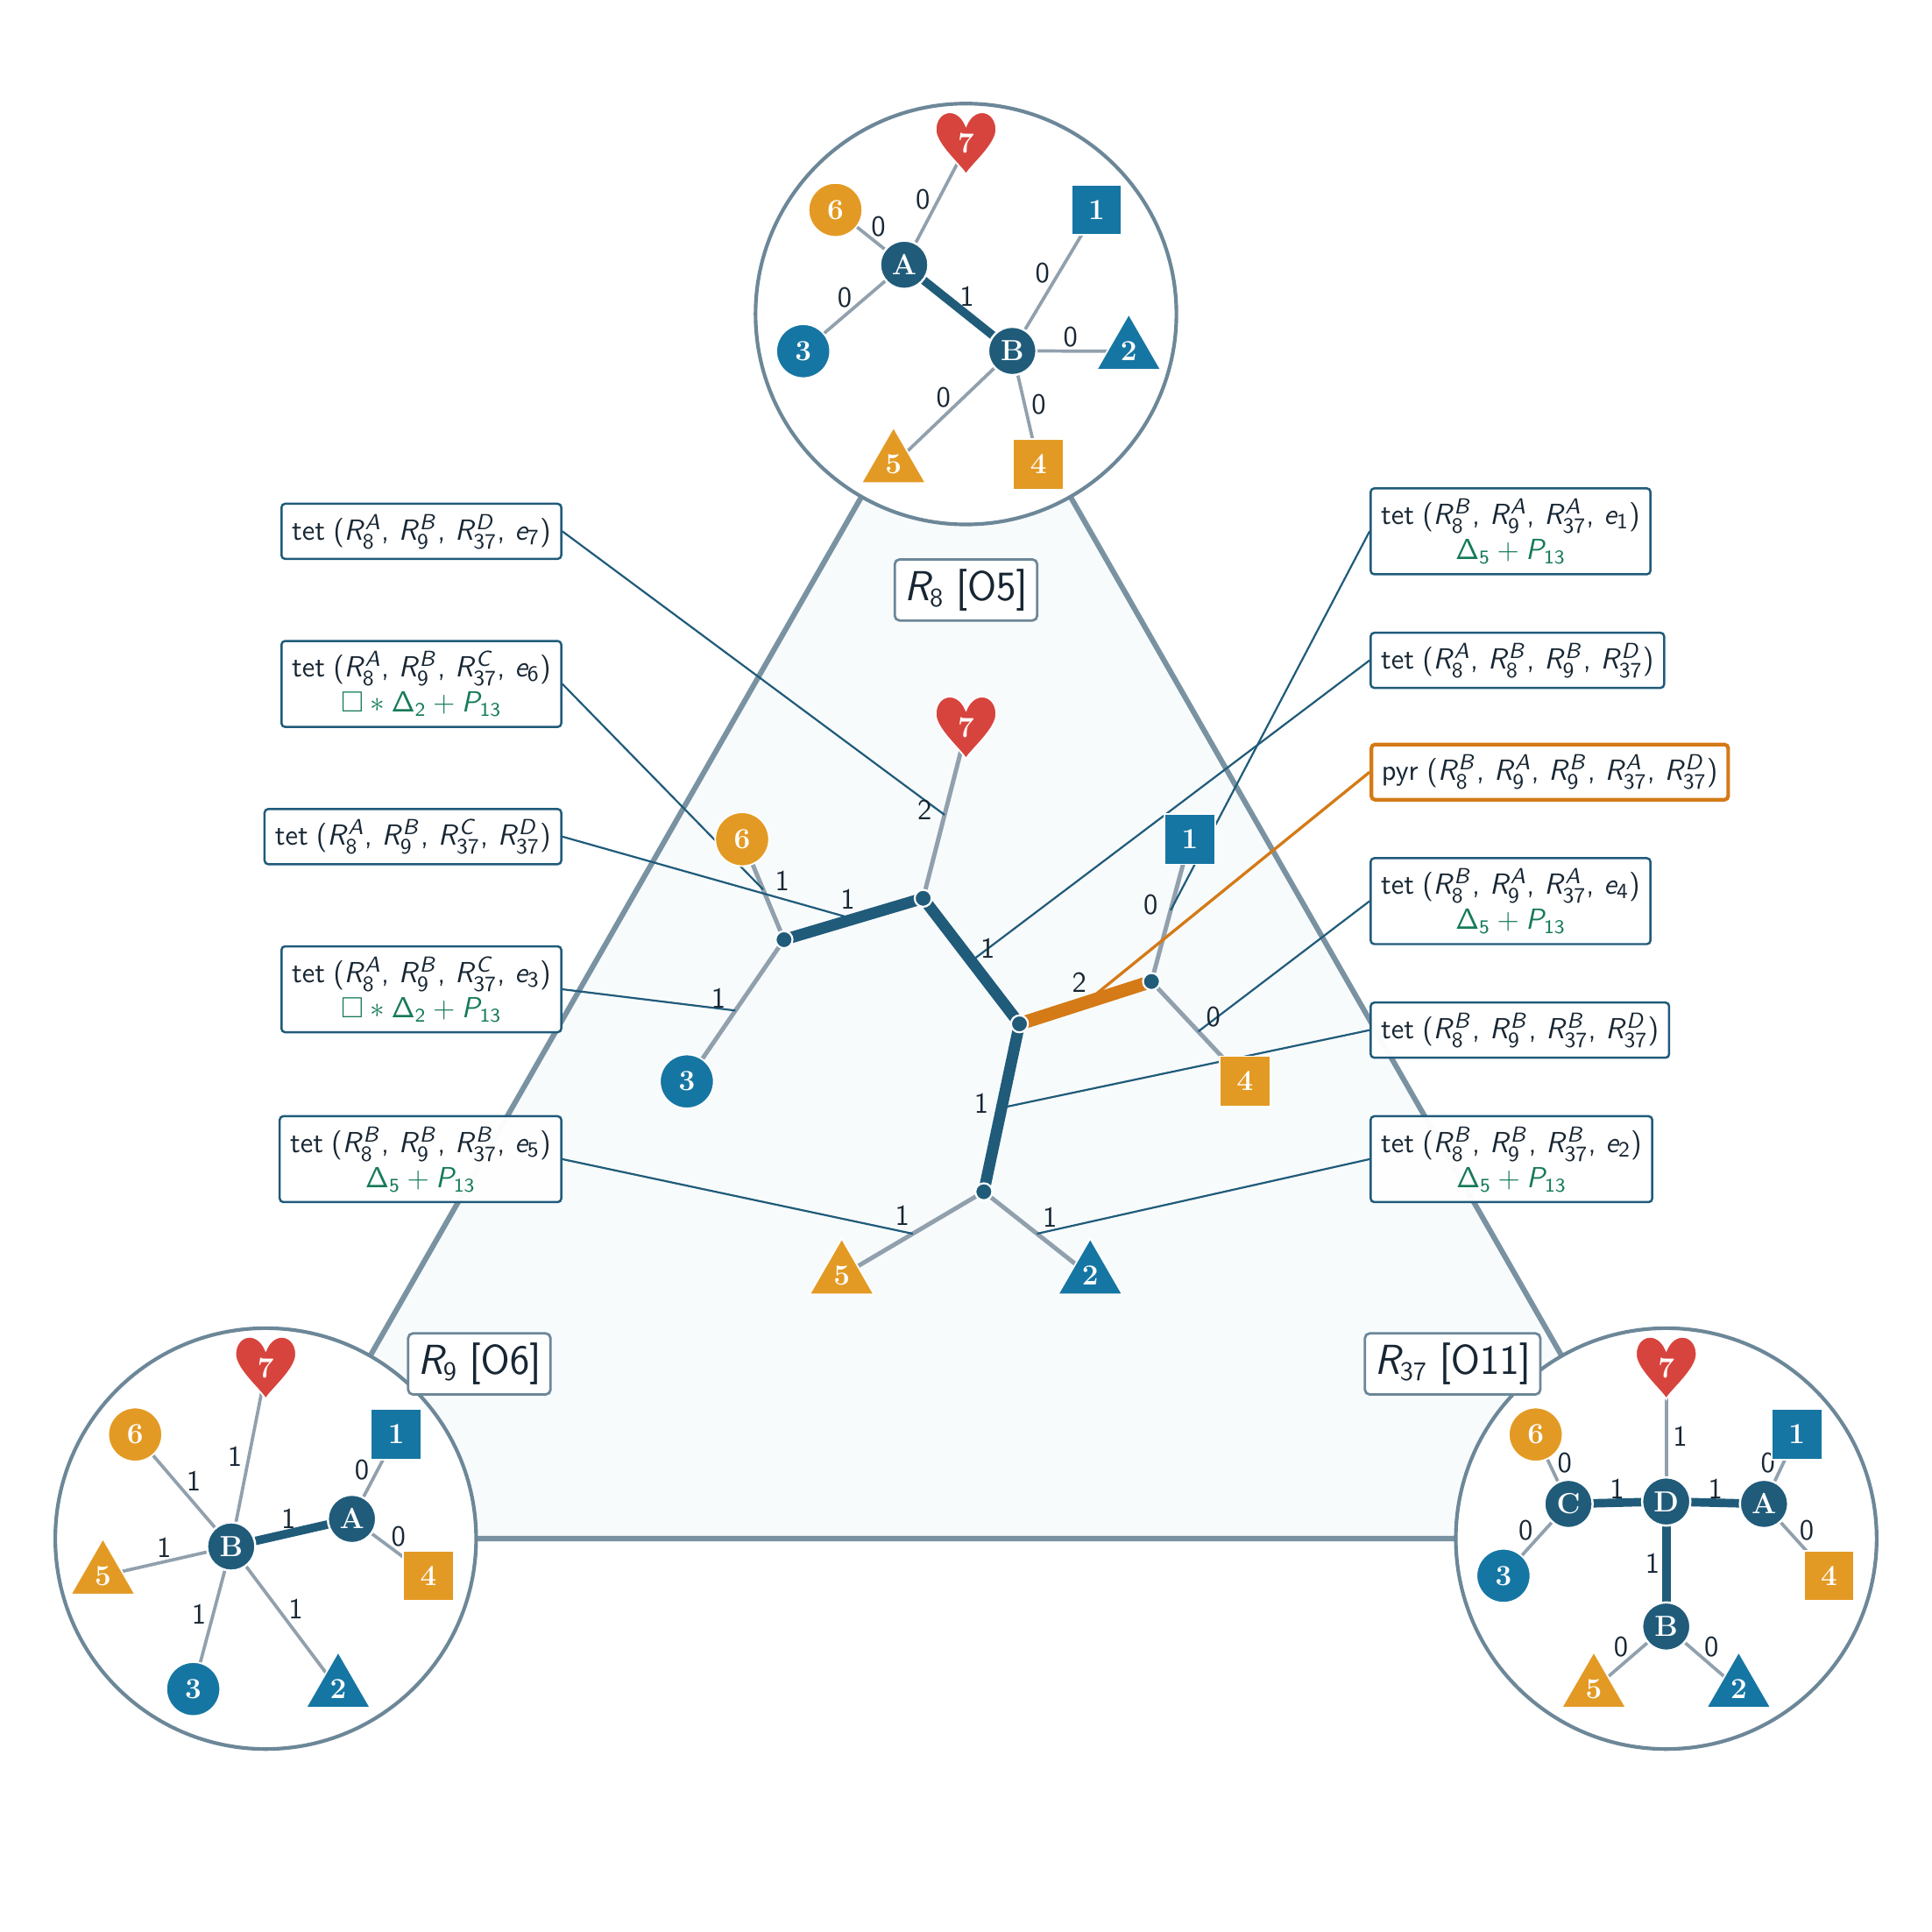
\begin{tikzpicture}[x=1cm,y=1cm]
\path[use as bounding box] (-13.65,-13.65) rectangle (13.65,13.65);
\path[support cell] (0.00000,9.45000)--(-10.15000,-8.30000)--(10.15000,-8.30000)--cycle;
\path[vertex disc] (0.00000,9.45000) circle[radius=3.05000cm];
\path[vertex disc] (-10.15000,-8.30000) circle[radius=3.05000cm];
\path[vertex disc] (10.15000,-8.30000) circle[radius=3.05000cm];
\coordinate (corner-1-v1) at (1.89203,10.95885);
\coordinate (corner-1-v2) at (2.35933,8.91150);
\coordinate (corner-1-v3) at (-2.35933,8.91150);
\coordinate (corner-1-v4) at (1.05000,7.26966);
\coordinate (corner-1-v5) at (-1.05000,7.26966);
\coordinate (corner-1-v6) at (-1.89203,10.95885);
\coordinate (corner-1-v7) at (0.00000,11.87000);
\coordinate (corner-1-v8) at (-0.89502,10.16376);
\coordinate (corner-1-v9) at (0.67127,8.91468);
\draw[internal edge] (corner-1-v8)--node[mini length,pos=0.5] {\(1\)}(corner-1-v9);
\draw[pendant edge] (corner-1-v1)--node[mini length,pos=0.5] {\(0\)}(corner-1-v9);
\draw[pendant edge] (corner-1-v2)--node[mini length,pos=0.5] {\(0\)}(corner-1-v9);
\draw[pendant edge] (corner-1-v3)--node[mini length,pos=0.5] {\(0\)}(corner-1-v8);
\draw[pendant edge] (corner-1-v4)--node[mini length,pos=0.5] {\(0\)}(corner-1-v9);
\draw[pendant edge] (corner-1-v5)--node[mini length,pos=0.5] {\(0\)}(corner-1-v9);
\draw[pendant edge] (corner-1-v6)--node[mini length,pos=0.5] {\(0\)}(corner-1-v8);
\draw[pendant edge] (corner-1-v7)--node[mini length,pos=0.5] {\(0\)}(corner-1-v8);
\node[lettered vertex] at (corner-1-v8) {A};
\node[lettered vertex] at (corner-1-v9) {B};
\taxonone{corner-1-v1}
\taxontwo{corner-1-v2}
\taxonthree{corner-1-v3}
\taxonfour{corner-1-v4}
\taxonfive{corner-1-v5}
\taxonsix{corner-1-v6}
\taxonseven{corner-1-v7}
\node[ray title] at (0.00000,5.45000) {\(R_{8}\;[\mathrm{O}5]\)};
\coordinate (corner-2-v1) at (-8.25797,-6.79115);
\coordinate (corner-2-v2) at (-9.10000,-10.48034);
\coordinate (corner-2-v3) at (-11.20000,-10.48034);
\coordinate (corner-2-v4) at (-7.79067,-8.83850);
\coordinate (corner-2-v5) at (-12.50933,-8.83850);
\coordinate (corner-2-v6) at (-12.04203,-6.79115);
\coordinate (corner-2-v7) at (-10.15000,-5.88000);
\coordinate (corner-2-v8) at (-8.89960,-8.01460);
\coordinate (corner-2-v9) at (-10.65016,-8.41416);
\draw[internal edge] (corner-2-v8)--node[mini length,pos=0.5] {\(1\)}(corner-2-v9);
\draw[pendant edge] (corner-2-v1)--node[mini length,pos=0.5] {\(0\)}(corner-2-v8);
\draw[pendant edge] (corner-2-v2)--node[mini length,pos=0.5] {\(1\)}(corner-2-v9);
\draw[pendant edge] (corner-2-v3)--node[mini length,pos=0.5] {\(1\)}(corner-2-v9);
\draw[pendant edge] (corner-2-v4)--node[mini length,pos=0.5] {\(0\)}(corner-2-v8);
\draw[pendant edge] (corner-2-v5)--node[mini length,pos=0.5] {\(1\)}(corner-2-v9);
\draw[pendant edge] (corner-2-v6)--node[mini length,pos=0.5] {\(1\)}(corner-2-v9);
\draw[pendant edge] (corner-2-v7)--node[mini length,pos=0.5] {\(1\)}(corner-2-v9);
\node[lettered vertex] at (corner-2-v8) {A};
\node[lettered vertex] at (corner-2-v9) {B};
\taxonone{corner-2-v1}
\taxontwo{corner-2-v2}
\taxonthree{corner-2-v3}
\taxonfour{corner-2-v4}
\taxonfive{corner-2-v5}
\taxonsix{corner-2-v6}
\taxonseven{corner-2-v7}
\node[ray title] at (-7.05349,-5.76788) {\(R_{9}\;[\mathrm{O}6]\)};
\coordinate (corner-3-v1) at (12.04203,-6.79115);
\coordinate (corner-3-v2) at (11.20000,-10.48034);
\coordinate (corner-3-v3) at (7.79067,-8.83850);
\coordinate (corner-3-v4) at (12.50933,-8.83850);
\coordinate (corner-3-v5) at (9.10000,-10.48034);
\coordinate (corner-3-v6) at (8.25797,-6.79115);
\coordinate (corner-3-v7) at (10.15000,-5.88000);
\coordinate (corner-3-v8) at (11.56712,-7.79729);
\coordinate (corner-3-v9) at (10.15000,-9.57430);
\coordinate (corner-3-v10) at (8.73288,-7.79729);
\coordinate (corner-3-v11) at (10.15000,-7.76222);
\draw[internal edge] (corner-3-v8)--node[mini length,pos=0.5] {\(1\)}(corner-3-v11);
\draw[internal edge] (corner-3-v9)--node[mini length,pos=0.5] {\(1\)}(corner-3-v11);
\draw[internal edge] (corner-3-v10)--node[mini length,pos=0.5] {\(1\)}(corner-3-v11);
\draw[pendant edge] (corner-3-v1)--node[mini length,pos=0.5] {\(0\)}(corner-3-v8);
\draw[pendant edge] (corner-3-v2)--node[mini length,pos=0.5] {\(0\)}(corner-3-v9);
\draw[pendant edge] (corner-3-v3)--node[mini length,pos=0.5] {\(0\)}(corner-3-v10);
\draw[pendant edge] (corner-3-v4)--node[mini length,pos=0.5] {\(0\)}(corner-3-v8);
\draw[pendant edge] (corner-3-v5)--node[mini length,pos=0.5] {\(0\)}(corner-3-v9);
\draw[pendant edge] (corner-3-v6)--node[mini length,pos=0.5] {\(0\)}(corner-3-v10);
\draw[pendant edge] (corner-3-v7)--node[mini length,pos=0.5] {\(1\)}(corner-3-v11);
\node[lettered vertex] at (corner-3-v8) {A};
\node[lettered vertex] at (corner-3-v9) {B};
\node[lettered vertex] at (corner-3-v10) {C};
\node[lettered vertex] at (corner-3-v11) {D};
\taxonone{corner-3-v1}
\taxontwo{corner-3-v2}
\taxonthree{corner-3-v3}
\taxonfour{corner-3-v4}
\taxonfive{corner-3-v5}
\taxonsix{corner-3-v6}
\taxonseven{corner-3-v7}
\node[ray title] at (7.05349,-5.76788) {\(R_{37}\;[\mathrm{O}11]\)};
\coordinate (central-v1) at (3.24460,1.83748);
\coordinate (central-v2) at (1.80062,-4.48902);
\coordinate (central-v3) at (-4.04595,-1.67346);
\coordinate (central-v4) at (4.04595,-1.67346);
\coordinate (central-v5) at (-1.80062,-4.48902);
\coordinate (central-v6) at (-3.24460,1.83748);
\coordinate (central-v7) at (0.00000,3.40000);
\coordinate (central-v8) at (2.68871,-0.22490);
\coordinate (central-v9) at (0.25853,-3.27226);
\coordinate (central-v10) at (-2.63701,0.38167);
\coordinate (central-v11) at (-0.62047,0.98098);
\coordinate (central-v12) at (0.77559,-0.83873);
\draw[central pyramid edge] (central-v8)--(central-v12);
\draw[central internal edge] (central-v9)--(central-v12);
\draw[central internal edge] (central-v10)--(central-v11);
\draw[central internal edge] (central-v11)--(central-v12);
\draw[central pendant edge] (central-v1)--(central-v8);
\draw[central pendant edge] (central-v2)--(central-v9);
\draw[central pendant edge] (central-v3)--(central-v10);
\draw[central pendant edge] (central-v4)--(central-v8);
\draw[central pendant edge] (central-v5)--(central-v9);
\draw[central pendant edge] (central-v6)--(central-v10);
\draw[central pendant edge] (central-v7)--(central-v11);
\draw[edge leader] (-5.85000,6.30000)--(-0.31024,2.19049);
\draw[edge leader] (-5.85000,4.08750)--(-2.94080,1.10957);
\draw[edge leader] (-5.85000,1.87500)--(-1.62874,0.68132);
\draw[edge leader] (-5.85000,-0.33750)--(-3.34148,-0.64590);
\draw[edge leader] (-5.85000,-2.80000)--(-0.77104,-3.88064);
\draw[edge leader] (5.85000,6.30000)--(2.96666,0.80629);
\draw[edge leader] (5.85000,4.43000)--(0.07756,0.07113);
\draw[pyramid leader] (5.85000,2.81000)--(1.73215,-0.53181);
\draw[edge leader] (5.85000,0.94000)--(3.36733,-0.94918);
\draw[edge leader] (5.85000,-0.93000)--(0.51706,-2.05549);
\draw[edge leader] (5.85000,-2.80000)--(1.02957,-3.88064);
\node[internal vertex] at (central-v8) {};
\node[internal vertex] at (central-v9) {};
\node[internal vertex] at (central-v10) {};
\node[internal vertex] at (central-v11) {};
\node[internal vertex] at (central-v12) {};
\taxonone{central-v1}
\taxontwo{central-v2}
\taxonthree{central-v3}
\taxonfour{central-v4}
\taxonfive{central-v5}
\taxonsix{central-v6}
\taxonseven{central-v7}
\path (central-v8)--node[central length,pos=.50] {\(2\)}(central-v12);
\path (central-v9)--node[central length,pos=.50] {\(1\)}(central-v12);
\path (central-v10)--node[central length,pos=.50] {\(1\)}(central-v11);
\path (central-v11)--node[central length,pos=.50] {\(1\)}(central-v12);
\path (central-v1)--node[central length,pos=.50] {\(0\)}(central-v8);
\path (central-v2)--node[central length,pos=.50] {\(1\)}(central-v9);
\path (central-v3)--node[central length,pos=.50] {\(1\)}(central-v10);
\path (central-v4)--node[central length,pos=.50] {\(0\)}(central-v8);
\path (central-v5)--node[central length,pos=.50] {\(1\)}(central-v9);
\path (central-v6)--node[central length,pos=.50] {\(1\)}(central-v10);
\path (central-v7)--node[central length,pos=.50] {\(2\)}(central-v11);
\node[edge callout,anchor=east] (callout-1) at (-5.85000,6.30000) {\(\mathrm{tet}\;(R_{8}^{A},\,R_{9}^{B},\,R_{37}^{D},\,e_{7})\)};
\node[edge callout,anchor=east] (callout-2) at (-5.85000,4.08750) {\(\mathrm{tet}\;(R_{8}^{A},\,R_{9}^{B},\,R_{37}^{C},\,e_{6})\)\\{\fontsize{12}{14}\selectfont\color{toricgreen}\(\square\ast\Delta_{2}+P_{13}\)}};
\node[edge callout,anchor=east] (callout-3) at (-5.85000,1.87500) {\(\mathrm{tet}\;(R_{8}^{A},\,R_{9}^{B},\,R_{37}^{C},\,R_{37}^{D})\)};
\node[edge callout,anchor=east] (callout-4) at (-5.85000,-0.33750) {\(\mathrm{tet}\;(R_{8}^{A},\,R_{9}^{B},\,R_{37}^{C},\,e_{3})\)\\{\fontsize{12}{14}\selectfont\color{toricgreen}\(\square\ast\Delta_{2}+P_{13}\)}};
\node[edge callout,anchor=east] (callout-5) at (-5.85000,-2.80000) {\(\mathrm{tet}\;(R_{8}^{B},\,R_{9}^{B},\,R_{37}^{B},\,e_{5})\)\\{\fontsize{12}{14}\selectfont\color{toricgreen}\(\Delta_{5}+P_{13}\)}};
\node[edge callout,anchor=west] (callout-6) at (5.85000,6.30000) {\(\mathrm{tet}\;(R_{8}^{B},\,R_{9}^{A},\,R_{37}^{A},\,e_{1})\)\\{\fontsize{12}{14}\selectfont\color{toricgreen}\(\Delta_{5}+P_{13}\)}};
\node[edge callout,anchor=west] (callout-7) at (5.85000,4.43000) {\(\mathrm{tet}\;(R_{8}^{A},\,R_{8}^{B},\,R_{9}^{B},\,R_{37}^{D})\)};
\node[pyramid callout,anchor=west] (callout-8) at (5.85000,2.81000) {\(\mathrm{pyr}\;(R_{8}^{B},\,R_{9}^{A},\,R_{9}^{B},\,R_{37}^{A},\,R_{37}^{D})\)};
\node[edge callout,anchor=west] (callout-9) at (5.85000,0.94000) {\(\mathrm{tet}\;(R_{8}^{B},\,R_{9}^{A},\,R_{37}^{A},\,e_{4})\)\\{\fontsize{12}{14}\selectfont\color{toricgreen}\(\Delta_{5}+P_{13}\)}};
\node[edge callout,anchor=west] (callout-10) at (5.85000,-0.93000) {\(\mathrm{tet}\;(R_{8}^{B},\,R_{9}^{B},\,R_{37}^{B},\,R_{37}^{D})\)};
\node[edge callout,anchor=west] (callout-11) at (5.85000,-2.80000) {\(\mathrm{tet}\;(R_{8}^{B},\,R_{9}^{B},\,R_{37}^{B},\,e_{2})\)\\{\fontsize{12}{14}\selectfont\color{toricgreen}\(\Delta_{5}+P_{13}\)}};
\end{tikzpicture}\end{center}\vspace{-1mm}
\begin{atlasbox}\begin{atlaspanel}
\textcolor{toricgreen}{\bfseries PRIME TORIC}\quad \(P_{13}\):\enspace \(\mathrm{AP}_{4}\ast\Delta_{1}\)\quad \(f=(10,33,50,37,12)\)\quad 15 lattice points
\end{atlaspanel}\end{atlasbox}
\clearpage
\begin{atlaspanel}[top=1mm,bottom=2mm]
\AtlasSupportOrbitSplit{%
\vspace*{-3mm}\mbox{{\LARGE\bfseries Triangle orbit 14}\hspace{3mm}\raisebox{.8mm}[0pt][0pt]{{\fontsize{16}{18}\selectfont\color{muted}size 3}}}%
}{%
\vspace*{-3mm}{\fontsize{13}{16}\selectfont{\color{muted}\(\mathbb{Q}\) and \(\mathbb{F}_2\)}\quad{\color{muted}\(\underline{\{8,\,30,\,37\}}\), \(\{10,\,33,\,37\}\), \(\{9,\,34,\,37\}\)}\rule[-3mm]{0pt}{3mm}}%
}%
\end{atlaspanel}\vspace{2mm}
\begin{center}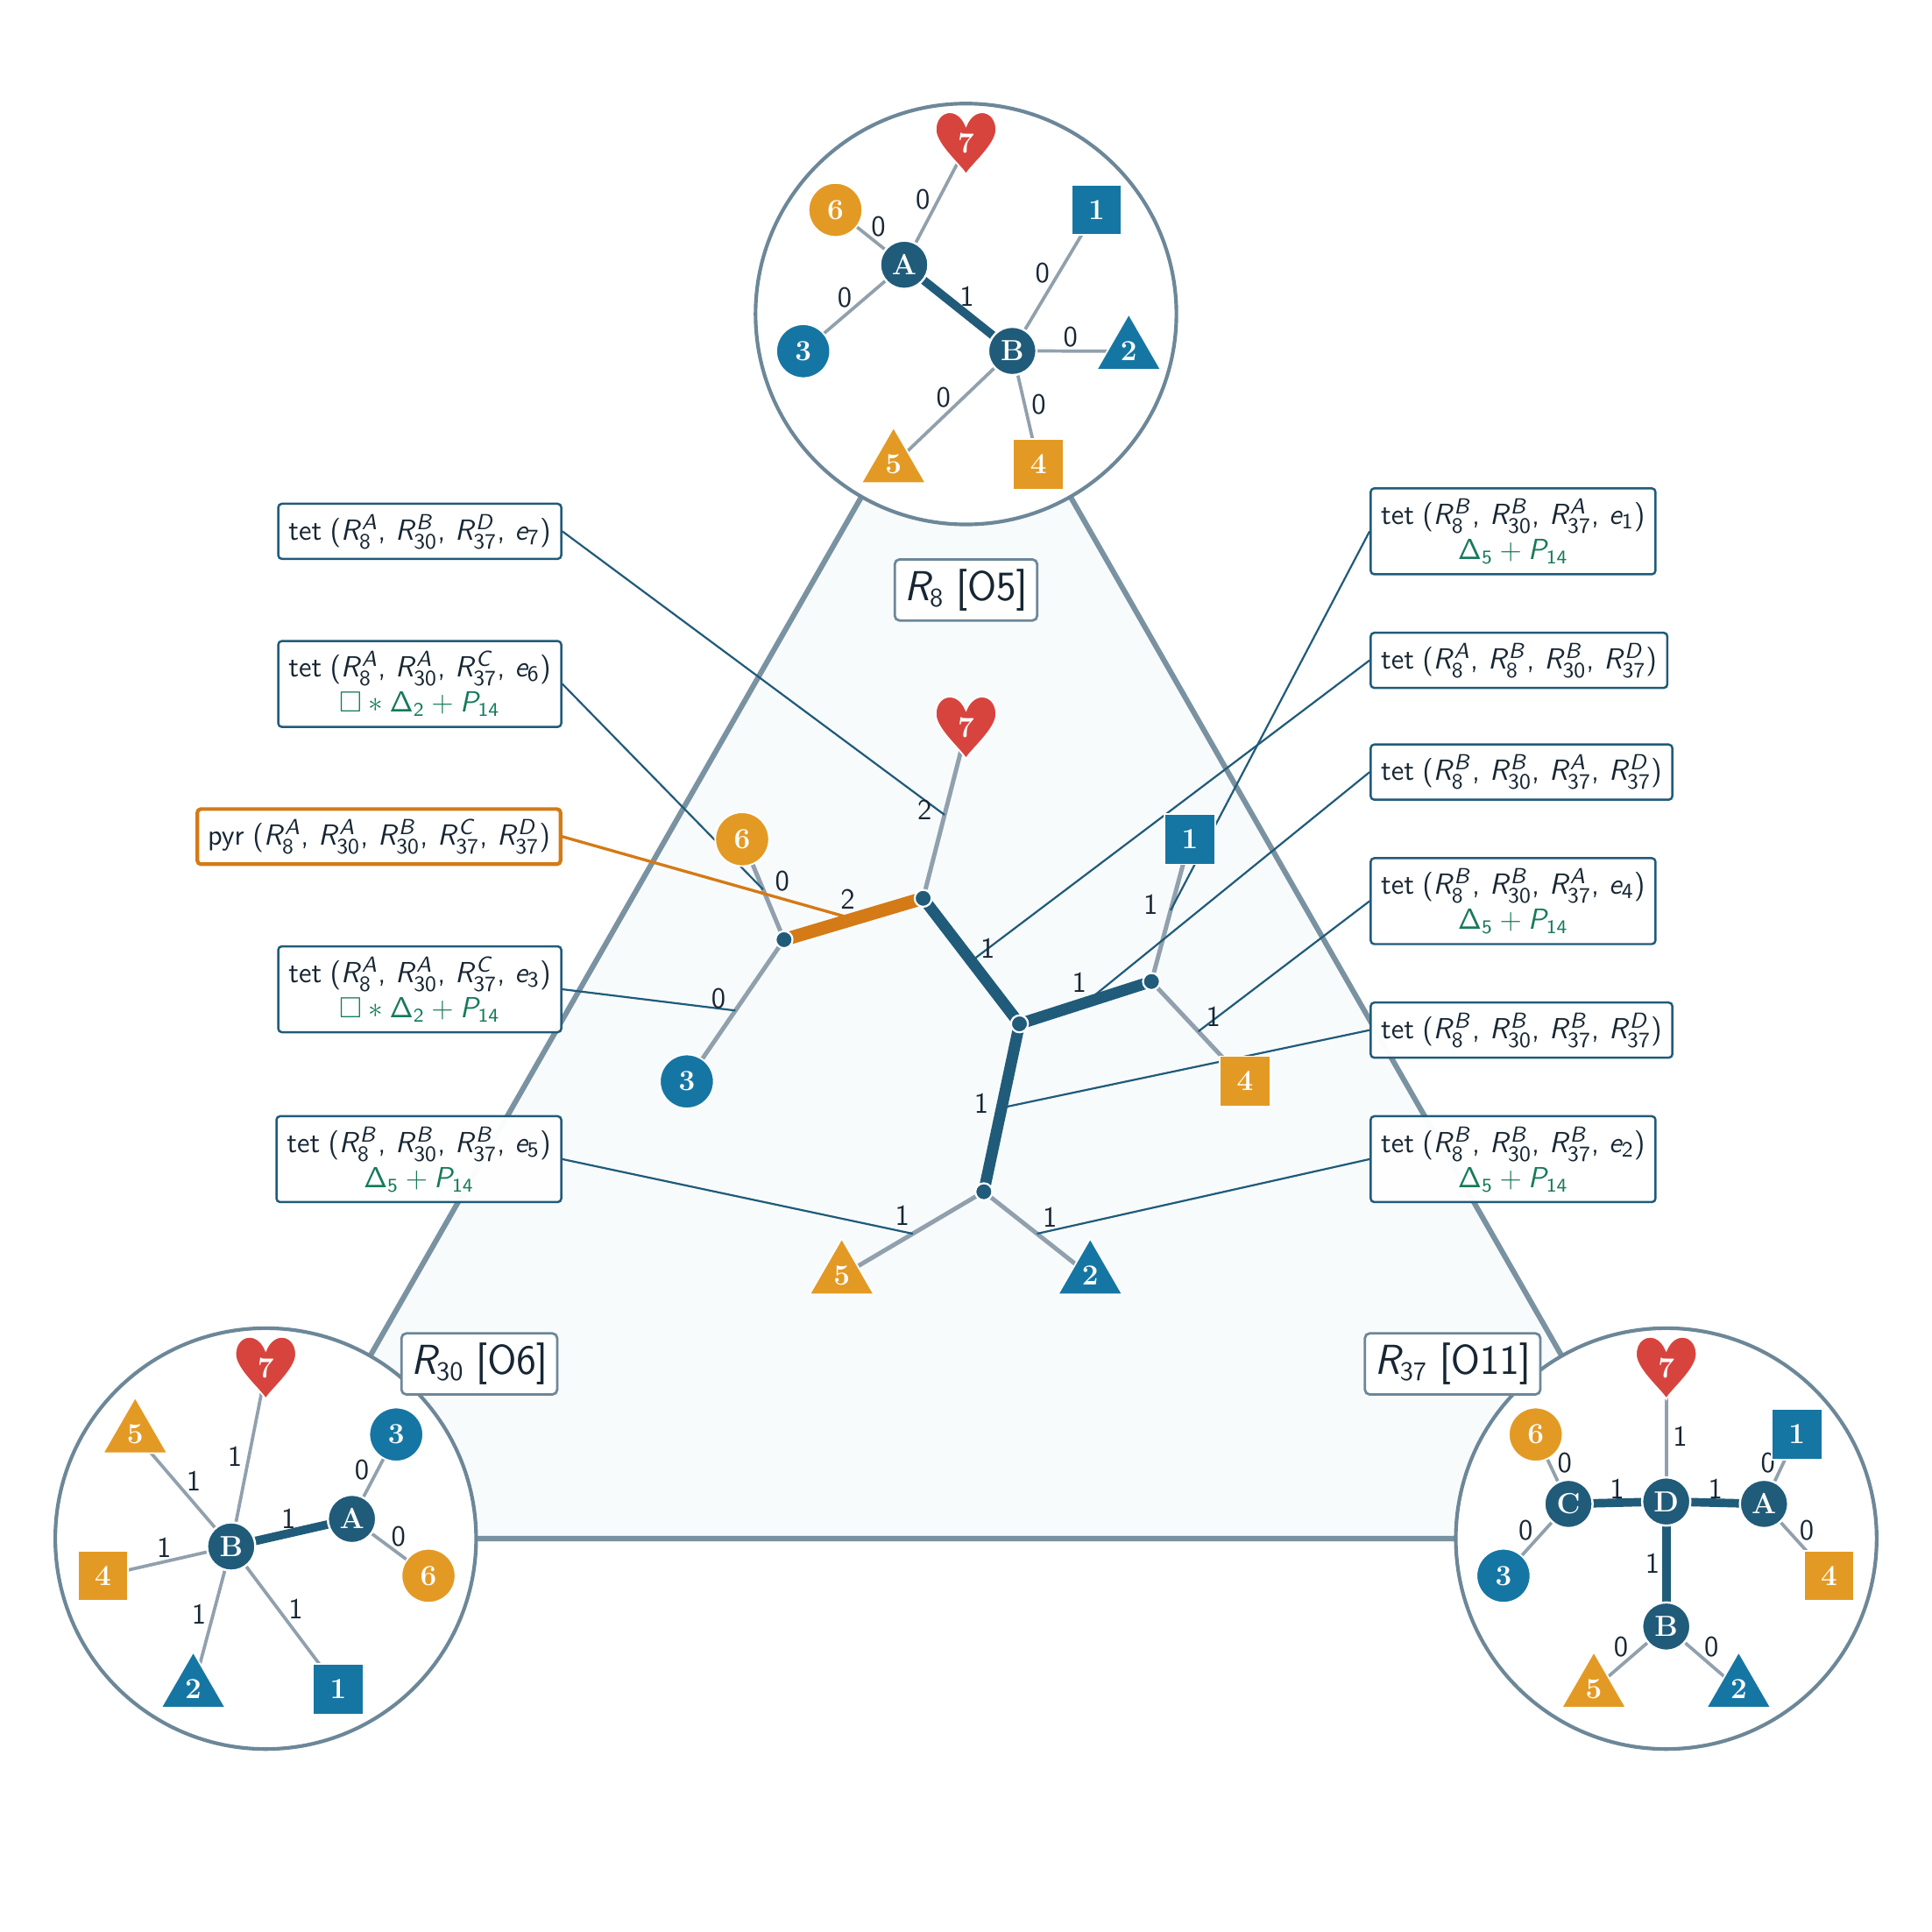
\begin{tikzpicture}[x=1cm,y=1cm]
\path[use as bounding box] (-13.65,-13.65) rectangle (13.65,13.65);
\path[support cell] (0.00000,9.45000)--(-10.15000,-8.30000)--(10.15000,-8.30000)--cycle;
\path[vertex disc] (0.00000,9.45000) circle[radius=3.05000cm];
\path[vertex disc] (-10.15000,-8.30000) circle[radius=3.05000cm];
\path[vertex disc] (10.15000,-8.30000) circle[radius=3.05000cm];
\coordinate (corner-1-v1) at (1.89203,10.95885);
\coordinate (corner-1-v2) at (2.35933,8.91150);
\coordinate (corner-1-v3) at (-2.35933,8.91150);
\coordinate (corner-1-v4) at (1.05000,7.26966);
\coordinate (corner-1-v5) at (-1.05000,7.26966);
\coordinate (corner-1-v6) at (-1.89203,10.95885);
\coordinate (corner-1-v7) at (0.00000,11.87000);
\coordinate (corner-1-v8) at (-0.89502,10.16376);
\coordinate (corner-1-v9) at (0.67127,8.91468);
\draw[internal edge] (corner-1-v8)--node[mini length,pos=0.5] {\(1\)}(corner-1-v9);
\draw[pendant edge] (corner-1-v1)--node[mini length,pos=0.5] {\(0\)}(corner-1-v9);
\draw[pendant edge] (corner-1-v2)--node[mini length,pos=0.5] {\(0\)}(corner-1-v9);
\draw[pendant edge] (corner-1-v3)--node[mini length,pos=0.5] {\(0\)}(corner-1-v8);
\draw[pendant edge] (corner-1-v4)--node[mini length,pos=0.5] {\(0\)}(corner-1-v9);
\draw[pendant edge] (corner-1-v5)--node[mini length,pos=0.5] {\(0\)}(corner-1-v9);
\draw[pendant edge] (corner-1-v6)--node[mini length,pos=0.5] {\(0\)}(corner-1-v8);
\draw[pendant edge] (corner-1-v7)--node[mini length,pos=0.5] {\(0\)}(corner-1-v8);
\node[lettered vertex] at (corner-1-v8) {A};
\node[lettered vertex] at (corner-1-v9) {B};
\taxonone{corner-1-v1}
\taxontwo{corner-1-v2}
\taxonthree{corner-1-v3}
\taxonfour{corner-1-v4}
\taxonfive{corner-1-v5}
\taxonsix{corner-1-v6}
\taxonseven{corner-1-v7}
\node[ray title] at (0.00000,5.45000) {\(R_{8}\;[\mathrm{O}5]\)};
\coordinate (corner-2-v1) at (-9.10000,-10.48034);
\coordinate (corner-2-v2) at (-11.20000,-10.48034);
\coordinate (corner-2-v3) at (-8.25797,-6.79115);
\coordinate (corner-2-v4) at (-12.50933,-8.83850);
\coordinate (corner-2-v5) at (-12.04203,-6.79115);
\coordinate (corner-2-v6) at (-7.79067,-8.83850);
\coordinate (corner-2-v7) at (-10.15000,-5.88000);
\coordinate (corner-2-v8) at (-8.89960,-8.01460);
\coordinate (corner-2-v9) at (-10.65016,-8.41416);
\draw[internal edge] (corner-2-v8)--node[mini length,pos=0.5] {\(1\)}(corner-2-v9);
\draw[pendant edge] (corner-2-v1)--node[mini length,pos=0.5] {\(1\)}(corner-2-v9);
\draw[pendant edge] (corner-2-v2)--node[mini length,pos=0.5] {\(1\)}(corner-2-v9);
\draw[pendant edge] (corner-2-v3)--node[mini length,pos=0.5] {\(0\)}(corner-2-v8);
\draw[pendant edge] (corner-2-v4)--node[mini length,pos=0.5] {\(1\)}(corner-2-v9);
\draw[pendant edge] (corner-2-v5)--node[mini length,pos=0.5] {\(1\)}(corner-2-v9);
\draw[pendant edge] (corner-2-v6)--node[mini length,pos=0.5] {\(0\)}(corner-2-v8);
\draw[pendant edge] (corner-2-v7)--node[mini length,pos=0.5] {\(1\)}(corner-2-v9);
\node[lettered vertex] at (corner-2-v8) {A};
\node[lettered vertex] at (corner-2-v9) {B};
\taxonone{corner-2-v1}
\taxontwo{corner-2-v2}
\taxonthree{corner-2-v3}
\taxonfour{corner-2-v4}
\taxonfive{corner-2-v5}
\taxonsix{corner-2-v6}
\taxonseven{corner-2-v7}
\node[ray title] at (-7.05349,-5.76788) {\(R_{30}\;[\mathrm{O}6]\)};
\coordinate (corner-3-v1) at (12.04203,-6.79115);
\coordinate (corner-3-v2) at (11.20000,-10.48034);
\coordinate (corner-3-v3) at (7.79067,-8.83850);
\coordinate (corner-3-v4) at (12.50933,-8.83850);
\coordinate (corner-3-v5) at (9.10000,-10.48034);
\coordinate (corner-3-v6) at (8.25797,-6.79115);
\coordinate (corner-3-v7) at (10.15000,-5.88000);
\coordinate (corner-3-v8) at (11.56712,-7.79729);
\coordinate (corner-3-v9) at (10.15000,-9.57430);
\coordinate (corner-3-v10) at (8.73288,-7.79729);
\coordinate (corner-3-v11) at (10.15000,-7.76222);
\draw[internal edge] (corner-3-v8)--node[mini length,pos=0.5] {\(1\)}(corner-3-v11);
\draw[internal edge] (corner-3-v9)--node[mini length,pos=0.5] {\(1\)}(corner-3-v11);
\draw[internal edge] (corner-3-v10)--node[mini length,pos=0.5] {\(1\)}(corner-3-v11);
\draw[pendant edge] (corner-3-v1)--node[mini length,pos=0.5] {\(0\)}(corner-3-v8);
\draw[pendant edge] (corner-3-v2)--node[mini length,pos=0.5] {\(0\)}(corner-3-v9);
\draw[pendant edge] (corner-3-v3)--node[mini length,pos=0.5] {\(0\)}(corner-3-v10);
\draw[pendant edge] (corner-3-v4)--node[mini length,pos=0.5] {\(0\)}(corner-3-v8);
\draw[pendant edge] (corner-3-v5)--node[mini length,pos=0.5] {\(0\)}(corner-3-v9);
\draw[pendant edge] (corner-3-v6)--node[mini length,pos=0.5] {\(0\)}(corner-3-v10);
\draw[pendant edge] (corner-3-v7)--node[mini length,pos=0.5] {\(1\)}(corner-3-v11);
\node[lettered vertex] at (corner-3-v8) {A};
\node[lettered vertex] at (corner-3-v9) {B};
\node[lettered vertex] at (corner-3-v10) {C};
\node[lettered vertex] at (corner-3-v11) {D};
\taxonone{corner-3-v1}
\taxontwo{corner-3-v2}
\taxonthree{corner-3-v3}
\taxonfour{corner-3-v4}
\taxonfive{corner-3-v5}
\taxonsix{corner-3-v6}
\taxonseven{corner-3-v7}
\node[ray title] at (7.05349,-5.76788) {\(R_{37}\;[\mathrm{O}11]\)};
\coordinate (central-v1) at (3.24460,1.83748);
\coordinate (central-v2) at (1.80062,-4.48902);
\coordinate (central-v3) at (-4.04595,-1.67346);
\coordinate (central-v4) at (4.04595,-1.67346);
\coordinate (central-v5) at (-1.80062,-4.48902);
\coordinate (central-v6) at (-3.24460,1.83748);
\coordinate (central-v7) at (0.00000,3.40000);
\coordinate (central-v8) at (-2.63701,0.38167);
\coordinate (central-v9) at (2.68871,-0.22490);
\coordinate (central-v10) at (0.25853,-3.27226);
\coordinate (central-v11) at (-0.62047,0.98098);
\coordinate (central-v12) at (0.77559,-0.83873);
\draw[central pyramid edge] (central-v8)--(central-v11);
\draw[central internal edge] (central-v9)--(central-v12);
\draw[central internal edge] (central-v10)--(central-v12);
\draw[central internal edge] (central-v11)--(central-v12);
\draw[central pendant edge] (central-v1)--(central-v9);
\draw[central pendant edge] (central-v2)--(central-v10);
\draw[central pendant edge] (central-v3)--(central-v8);
\draw[central pendant edge] (central-v4)--(central-v9);
\draw[central pendant edge] (central-v5)--(central-v10);
\draw[central pendant edge] (central-v6)--(central-v8);
\draw[central pendant edge] (central-v7)--(central-v11);
\draw[edge leader] (-5.85000,6.30000)--(-0.31024,2.19049);
\draw[edge leader] (-5.85000,4.08750)--(-2.94080,1.10957);
\draw[pyramid leader] (-5.85000,1.87500)--(-1.62874,0.68132);
\draw[edge leader] (-5.85000,-0.33750)--(-3.34148,-0.64590);
\draw[edge leader] (-5.85000,-2.80000)--(-0.77104,-3.88064);
\draw[edge leader] (5.85000,6.30000)--(2.96666,0.80629);
\draw[edge leader] (5.85000,4.43000)--(0.07756,0.07113);
\draw[edge leader] (5.85000,2.81000)--(1.73215,-0.53181);
\draw[edge leader] (5.85000,0.94000)--(3.36733,-0.94918);
\draw[edge leader] (5.85000,-0.93000)--(0.51706,-2.05549);
\draw[edge leader] (5.85000,-2.80000)--(1.02957,-3.88064);
\node[internal vertex] at (central-v8) {};
\node[internal vertex] at (central-v9) {};
\node[internal vertex] at (central-v10) {};
\node[internal vertex] at (central-v11) {};
\node[internal vertex] at (central-v12) {};
\taxonone{central-v1}
\taxontwo{central-v2}
\taxonthree{central-v3}
\taxonfour{central-v4}
\taxonfive{central-v5}
\taxonsix{central-v6}
\taxonseven{central-v7}
\path (central-v8)--node[central length,pos=.50] {\(2\)}(central-v11);
\path (central-v9)--node[central length,pos=.50] {\(1\)}(central-v12);
\path (central-v10)--node[central length,pos=.50] {\(1\)}(central-v12);
\path (central-v11)--node[central length,pos=.50] {\(1\)}(central-v12);
\path (central-v1)--node[central length,pos=.50] {\(1\)}(central-v9);
\path (central-v2)--node[central length,pos=.50] {\(1\)}(central-v10);
\path (central-v3)--node[central length,pos=.50] {\(0\)}(central-v8);
\path (central-v4)--node[central length,pos=.50] {\(1\)}(central-v9);
\path (central-v5)--node[central length,pos=.50] {\(1\)}(central-v10);
\path (central-v6)--node[central length,pos=.50] {\(0\)}(central-v8);
\path (central-v7)--node[central length,pos=.50] {\(2\)}(central-v11);
\node[edge callout,anchor=east] (callout-1) at (-5.85000,6.30000) {\(\mathrm{tet}\;(R_{8}^{A},\,R_{30}^{B},\,R_{37}^{D},\,e_{7})\)};
\node[edge callout,anchor=east] (callout-2) at (-5.85000,4.08750) {\(\mathrm{tet}\;(R_{8}^{A},\,R_{30}^{A},\,R_{37}^{C},\,e_{6})\)\\{\fontsize{12}{14}\selectfont\color{toricgreen}\(\square\ast\Delta_{2}+P_{14}\)}};
\node[pyramid callout,anchor=east] (callout-3) at (-5.85000,1.87500) {\(\mathrm{pyr}\;(R_{8}^{A},\,R_{30}^{A},\,R_{30}^{B},\,R_{37}^{C},\,R_{37}^{D})\)};
\node[edge callout,anchor=east] (callout-4) at (-5.85000,-0.33750) {\(\mathrm{tet}\;(R_{8}^{A},\,R_{30}^{A},\,R_{37}^{C},\,e_{3})\)\\{\fontsize{12}{14}\selectfont\color{toricgreen}\(\square\ast\Delta_{2}+P_{14}\)}};
\node[edge callout,anchor=east] (callout-5) at (-5.85000,-2.80000) {\(\mathrm{tet}\;(R_{8}^{B},\,R_{30}^{B},\,R_{37}^{B},\,e_{5})\)\\{\fontsize{12}{14}\selectfont\color{toricgreen}\(\Delta_{5}+P_{14}\)}};
\node[edge callout,anchor=west] (callout-6) at (5.85000,6.30000) {\(\mathrm{tet}\;(R_{8}^{B},\,R_{30}^{B},\,R_{37}^{A},\,e_{1})\)\\{\fontsize{12}{14}\selectfont\color{toricgreen}\(\Delta_{5}+P_{14}\)}};
\node[edge callout,anchor=west] (callout-7) at (5.85000,4.43000) {\(\mathrm{tet}\;(R_{8}^{A},\,R_{8}^{B},\,R_{30}^{B},\,R_{37}^{D})\)};
\node[edge callout,anchor=west] (callout-8) at (5.85000,2.81000) {\(\mathrm{tet}\;(R_{8}^{B},\,R_{30}^{B},\,R_{37}^{A},\,R_{37}^{D})\)};
\node[edge callout,anchor=west] (callout-9) at (5.85000,0.94000) {\(\mathrm{tet}\;(R_{8}^{B},\,R_{30}^{B},\,R_{37}^{A},\,e_{4})\)\\{\fontsize{12}{14}\selectfont\color{toricgreen}\(\Delta_{5}+P_{14}\)}};
\node[edge callout,anchor=west] (callout-10) at (5.85000,-0.93000) {\(\mathrm{tet}\;(R_{8}^{B},\,R_{30}^{B},\,R_{37}^{B},\,R_{37}^{D})\)};
\node[edge callout,anchor=west] (callout-11) at (5.85000,-2.80000) {\(\mathrm{tet}\;(R_{8}^{B},\,R_{30}^{B},\,R_{37}^{B},\,e_{2})\)\\{\fontsize{12}{14}\selectfont\color{toricgreen}\(\Delta_{5}+P_{14}\)}};
\end{tikzpicture}\end{center}\vspace{-1mm}
\begin{atlasbox}\begin{atlaspanel}
\textcolor{toricgreen}{\bfseries PRIME TORIC}\quad \(P_{14}\):\enspace \(\mathrm{AP}_{4}\ast\Delta_{1}\)\quad \(f=(10,33,50,37,12)\)\quad 15 lattice points
\end{atlaspanel}\end{atlasbox}
\clearpage
\begin{atlaspanel}[top=1mm,bottom=2mm]
\AtlasSupportOrbitSplit{%
\vspace*{-3mm}\mbox{{\LARGE\bfseries Triangle orbit 15}\hspace{3mm}\raisebox{.8mm}[0pt][0pt]{{\fontsize{16}{18}\selectfont\color{muted}size 12}}}%
}{%
\vspace*{-3mm}{\fontsize{13}{16}\selectfont{\color{muted}\(\mathbb{Q}\) and \(\mathbb{F}_2\)}\quad{\color{muted}\(\underline{\{1,\,3,\,9\}}\), \(\{4,\,5,\,10\}\), \(\{3,\,9,\,23\}\), \(\{5,\,10,\,24\}\), \(\{16,\,30,\,38\}\), \(\{16,\,30,\,39\}\), \(\{27,\,30,\,48\}\), \(\{27,\,30,\,49\}\), \(\{10,\,42,\,46\}\), \(\{9,\,43,\,47\}\), \(\{10,\,46,\,51\}\), \(\{9,\,47,\,50\}\)}\rule[-3mm]{0pt}{3mm}}%
}%
\end{atlaspanel}\vspace{2mm}
\begin{center}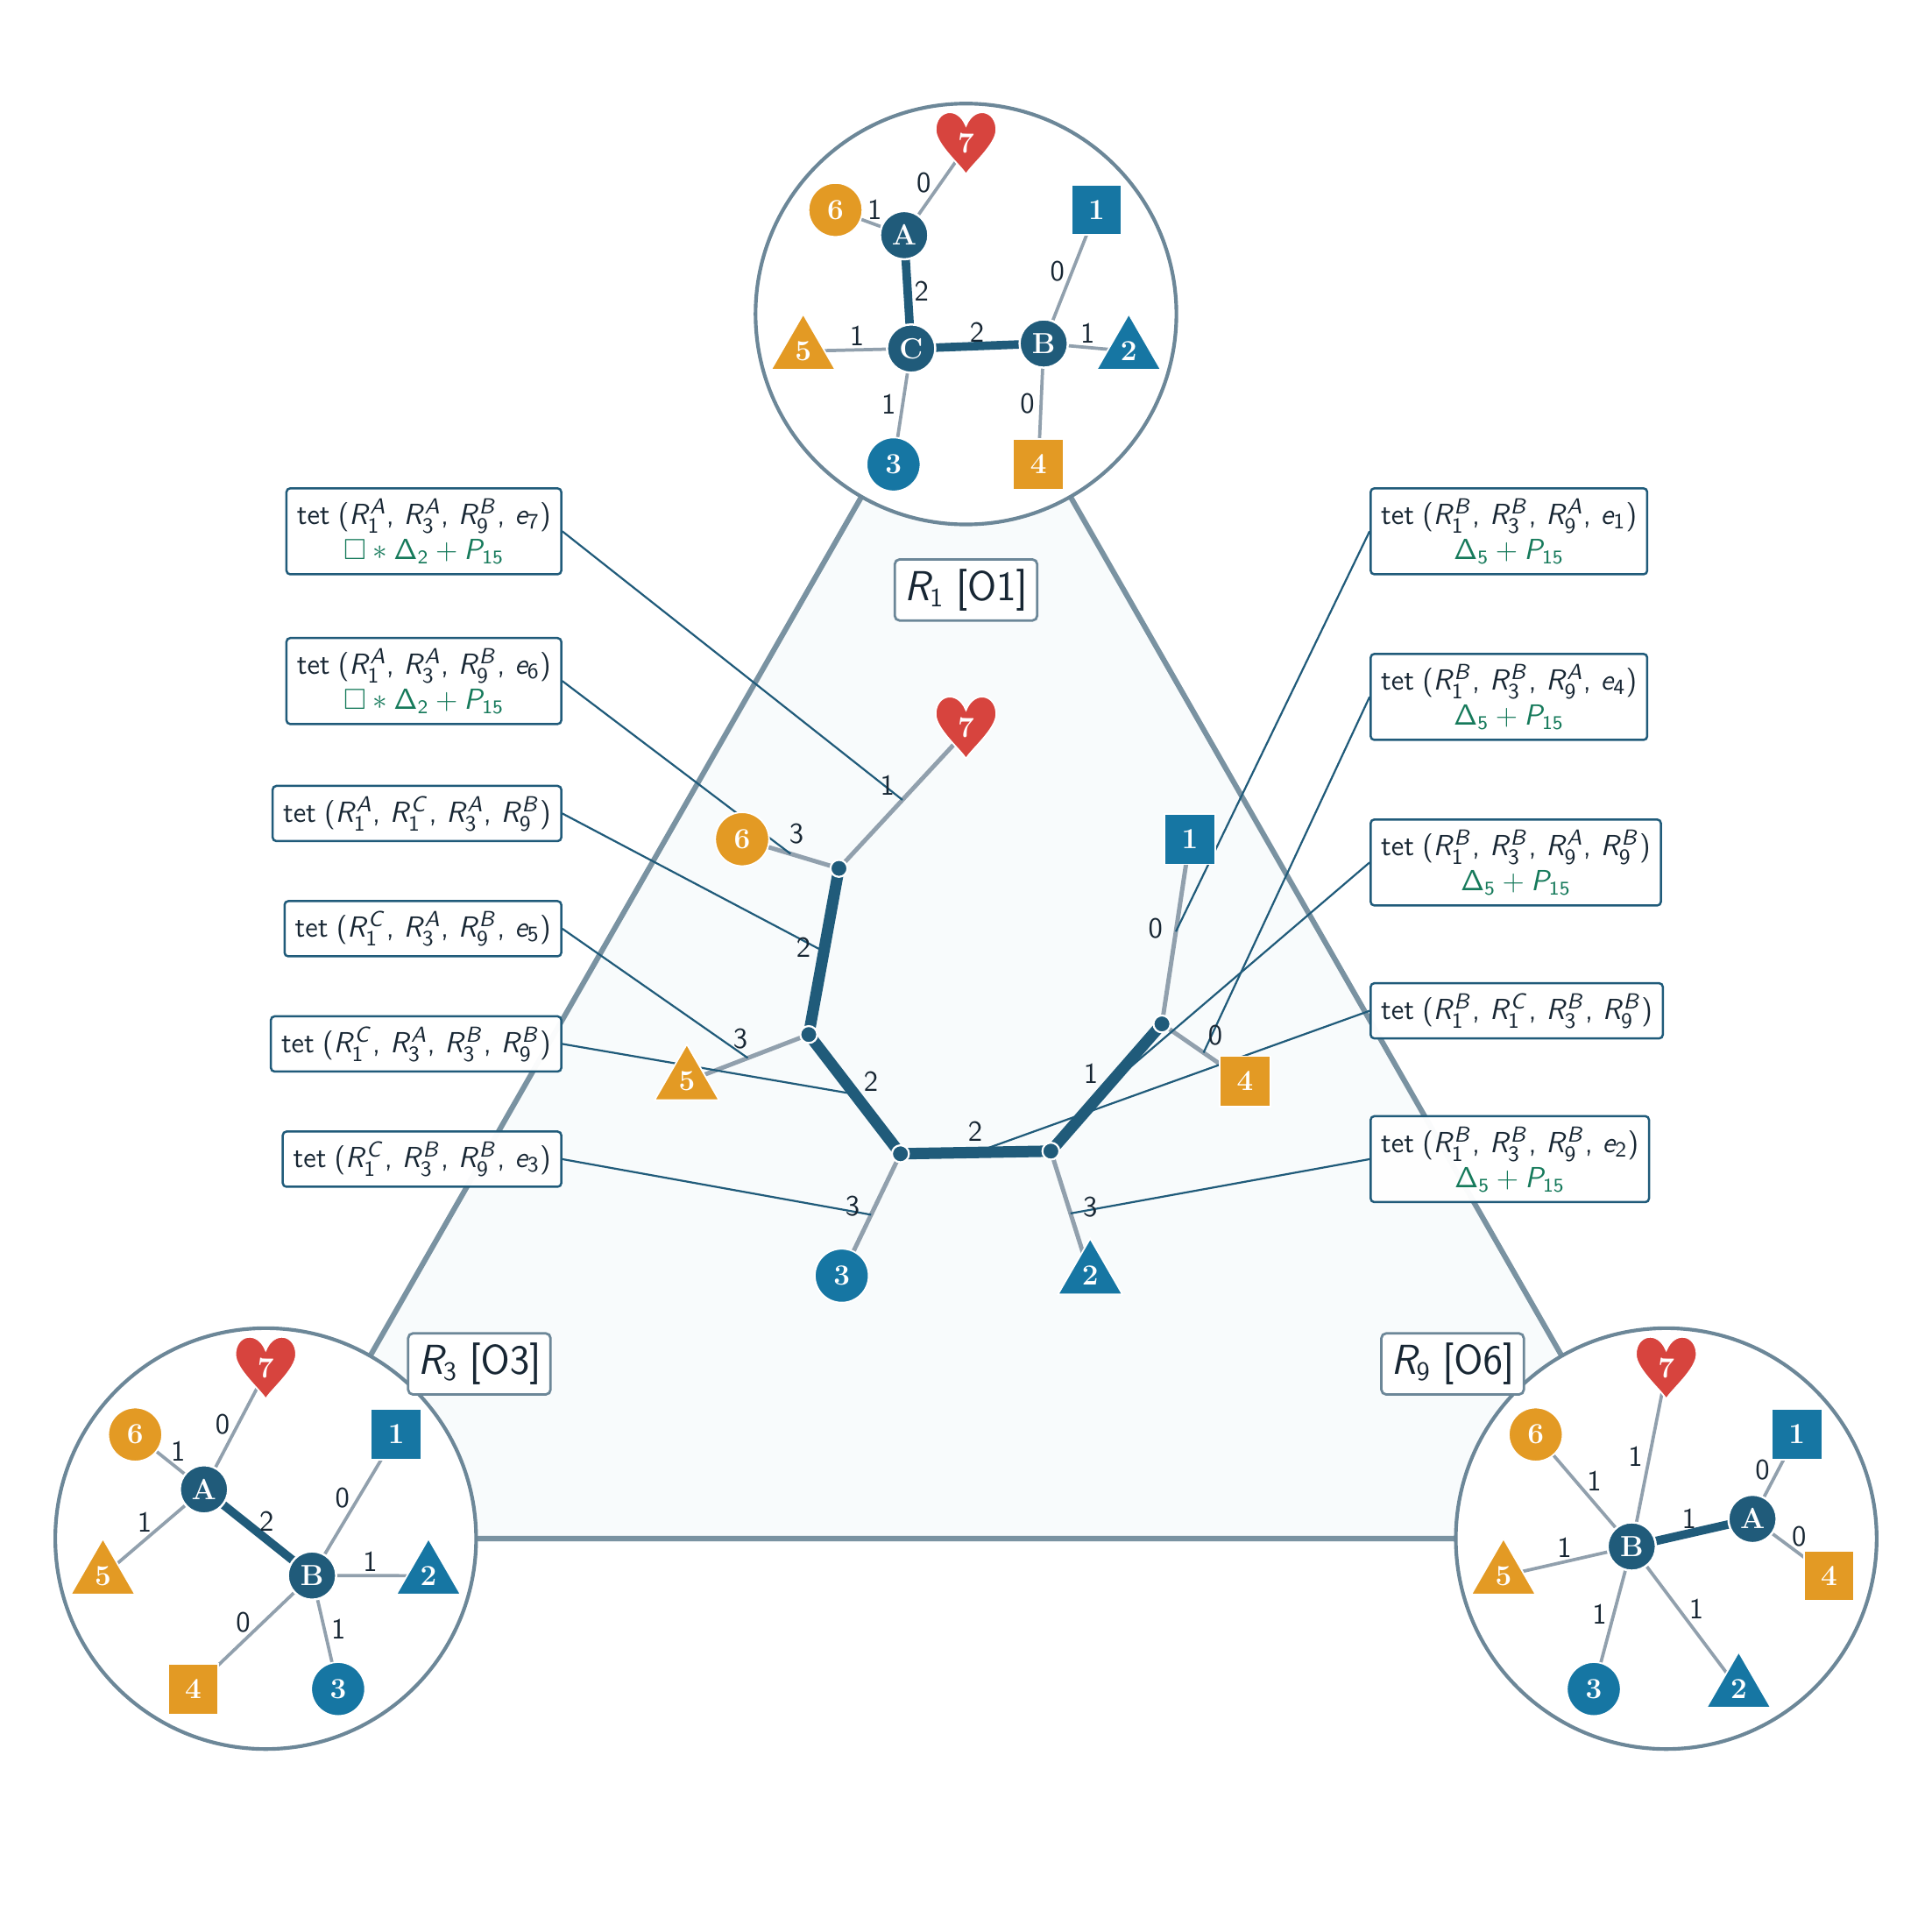
\begin{tikzpicture}[x=1cm,y=1cm]
\path[use as bounding box] (-13.65,-13.65) rectangle (13.65,13.65);
\path[support cell] (0.00000,9.45000)--(-10.15000,-8.30000)--(10.15000,-8.30000)--cycle;
\path[vertex disc] (0.00000,9.45000) circle[radius=3.05000cm];
\path[vertex disc] (-10.15000,-8.30000) circle[radius=3.05000cm];
\path[vertex disc] (10.15000,-8.30000) circle[radius=3.05000cm];
\coordinate (corner-1-v1) at (1.89203,10.95885);
\coordinate (corner-1-v2) at (2.35933,8.91150);
\coordinate (corner-1-v3) at (-1.05000,7.26966);
\coordinate (corner-1-v4) at (1.05000,7.26966);
\coordinate (corner-1-v5) at (-2.35933,8.91150);
\coordinate (corner-1-v6) at (-1.89203,10.95885);
\coordinate (corner-1-v7) at (0.00000,11.87000);
\coordinate (corner-1-v8) at (-0.89552,10.59262);
\coordinate (corner-1-v9) at (1.12671,9.02225);
\coordinate (corner-1-v10) at (-0.79454,8.94901);
\draw[internal edge] (corner-1-v8)--node[mini length,pos=0.5] {\(2\)}(corner-1-v10);
\draw[internal edge] (corner-1-v9)--node[mini length,pos=0.5] {\(2\)}(corner-1-v10);
\draw[pendant edge] (corner-1-v1)--node[mini length,pos=0.5] {\(0\)}(corner-1-v9);
\draw[pendant edge] (corner-1-v2)--node[mini length,pos=0.5] {\(1\)}(corner-1-v9);
\draw[pendant edge] (corner-1-v3)--node[mini length,pos=0.5] {\(1\)}(corner-1-v10);
\draw[pendant edge] (corner-1-v4)--node[mini length,pos=0.5] {\(0\)}(corner-1-v9);
\draw[pendant edge] (corner-1-v5)--node[mini length,pos=0.5] {\(1\)}(corner-1-v10);
\draw[pendant edge] (corner-1-v6)--node[mini length,pos=0.5] {\(1\)}(corner-1-v8);
\draw[pendant edge] (corner-1-v7)--node[mini length,pos=0.5] {\(0\)}(corner-1-v8);
\node[lettered vertex] at (corner-1-v8) {A};
\node[lettered vertex] at (corner-1-v9) {B};
\node[lettered vertex] at (corner-1-v10) {C};
\taxonone{corner-1-v1}
\taxontwo{corner-1-v2}
\taxonthree{corner-1-v3}
\taxonfour{corner-1-v4}
\taxonfive{corner-1-v5}
\taxonsix{corner-1-v6}
\taxonseven{corner-1-v7}
\node[ray title] at (0.00000,5.45000) {\(R_{1}\;[\mathrm{O}1]\)};
\coordinate (corner-2-v1) at (-8.25797,-6.79115);
\coordinate (corner-2-v2) at (-7.79067,-8.83850);
\coordinate (corner-2-v3) at (-9.10000,-10.48034);
\coordinate (corner-2-v4) at (-11.20000,-10.48034);
\coordinate (corner-2-v5) at (-12.50933,-8.83850);
\coordinate (corner-2-v6) at (-12.04203,-6.79115);
\coordinate (corner-2-v7) at (-10.15000,-5.88000);
\coordinate (corner-2-v8) at (-11.04502,-7.58624);
\coordinate (corner-2-v9) at (-9.47873,-8.83532);
\draw[internal edge] (corner-2-v8)--node[mini length,pos=0.5] {\(2\)}(corner-2-v9);
\draw[pendant edge] (corner-2-v1)--node[mini length,pos=0.5] {\(0\)}(corner-2-v9);
\draw[pendant edge] (corner-2-v2)--node[mini length,pos=0.5] {\(1\)}(corner-2-v9);
\draw[pendant edge] (corner-2-v3)--node[mini length,pos=0.5] {\(1\)}(corner-2-v9);
\draw[pendant edge] (corner-2-v4)--node[mini length,pos=0.5] {\(0\)}(corner-2-v9);
\draw[pendant edge] (corner-2-v5)--node[mini length,pos=0.5] {\(1\)}(corner-2-v8);
\draw[pendant edge] (corner-2-v6)--node[mini length,pos=0.5] {\(1\)}(corner-2-v8);
\draw[pendant edge] (corner-2-v7)--node[mini length,pos=0.5] {\(0\)}(corner-2-v8);
\node[lettered vertex] at (corner-2-v8) {A};
\node[lettered vertex] at (corner-2-v9) {B};
\taxonone{corner-2-v1}
\taxontwo{corner-2-v2}
\taxonthree{corner-2-v3}
\taxonfour{corner-2-v4}
\taxonfive{corner-2-v5}
\taxonsix{corner-2-v6}
\taxonseven{corner-2-v7}
\node[ray title] at (-7.05349,-5.76788) {\(R_{3}\;[\mathrm{O}3]\)};
\coordinate (corner-3-v1) at (12.04203,-6.79115);
\coordinate (corner-3-v2) at (11.20000,-10.48034);
\coordinate (corner-3-v3) at (9.10000,-10.48034);
\coordinate (corner-3-v4) at (12.50933,-8.83850);
\coordinate (corner-3-v5) at (7.79067,-8.83850);
\coordinate (corner-3-v6) at (8.25797,-6.79115);
\coordinate (corner-3-v7) at (10.15000,-5.88000);
\coordinate (corner-3-v8) at (11.40040,-8.01460);
\coordinate (corner-3-v9) at (9.64984,-8.41416);
\draw[internal edge] (corner-3-v8)--node[mini length,pos=0.5] {\(1\)}(corner-3-v9);
\draw[pendant edge] (corner-3-v1)--node[mini length,pos=0.5] {\(0\)}(corner-3-v8);
\draw[pendant edge] (corner-3-v2)--node[mini length,pos=0.5] {\(1\)}(corner-3-v9);
\draw[pendant edge] (corner-3-v3)--node[mini length,pos=0.5] {\(1\)}(corner-3-v9);
\draw[pendant edge] (corner-3-v4)--node[mini length,pos=0.5] {\(0\)}(corner-3-v8);
\draw[pendant edge] (corner-3-v5)--node[mini length,pos=0.5] {\(1\)}(corner-3-v9);
\draw[pendant edge] (corner-3-v6)--node[mini length,pos=0.5] {\(1\)}(corner-3-v9);
\draw[pendant edge] (corner-3-v7)--node[mini length,pos=0.5] {\(1\)}(corner-3-v9);
\node[lettered vertex] at (corner-3-v8) {A};
\node[lettered vertex] at (corner-3-v9) {B};
\taxonone{corner-3-v1}
\taxontwo{corner-3-v2}
\taxonthree{corner-3-v3}
\taxonfour{corner-3-v4}
\taxonfive{corner-3-v5}
\taxonsix{corner-3-v6}
\taxonseven{corner-3-v7}
\node[ray title] at (7.05349,-5.76788) {\(R_{9}\;[\mathrm{O}6]\)};
\coordinate (central-v1) at (3.24460,1.83748);
\coordinate (central-v2) at (1.80062,-4.48902);
\coordinate (central-v3) at (-1.80062,-4.48902);
\coordinate (central-v4) at (4.04595,-1.67346);
\coordinate (central-v5) at (-4.04595,-1.67346);
\coordinate (central-v6) at (-3.24460,1.83748);
\coordinate (central-v7) at (0.00000,3.40000);
\coordinate (central-v8) at (-1.84118,1.41461);
\coordinate (central-v9) at (-2.27895,-0.99366);
\coordinate (central-v10) at (-0.94972,-2.72212);
\coordinate (central-v11) at (2.84032,-0.83988);
\coordinate (central-v12) at (1.23040,-2.68367);
\draw[central internal edge] (central-v8)--(central-v9);
\draw[central internal edge] (central-v9)--(central-v10);
\draw[central internal edge] (central-v10)--(central-v12);
\draw[central internal edge] (central-v11)--(central-v12);
\draw[central pendant edge] (central-v1)--(central-v11);
\draw[central pendant edge] (central-v2)--(central-v12);
\draw[central pendant edge] (central-v3)--(central-v10);
\draw[central pendant edge] (central-v4)--(central-v11);
\draw[central pendant edge] (central-v5)--(central-v9);
\draw[central pendant edge] (central-v6)--(central-v8);
\draw[central pendant edge] (central-v7)--(central-v8);
\draw[edge leader] (-5.85000,6.30000)--(-0.92059,2.40730);
\draw[edge leader] (-5.85000,4.13000)--(-2.54289,1.62605);
\draw[edge leader] (-5.85000,2.21000)--(-2.06007,0.21048);
\draw[edge leader] (-5.85000,0.54000)--(-3.16245,-1.33356);
\draw[edge leader] (-5.85000,-1.13000)--(-1.61434,-1.85789);
\draw[edge leader] (-5.85000,-2.80000)--(-1.37517,-3.60557);
\draw[edge leader] (5.85000,6.30000)--(3.04246,0.49880);
\draw[edge leader] (5.85000,3.90000)--(3.44313,-1.25667);
\draw[edge leader] (5.85000,1.50000)--(2.03536,-1.76178);
\draw[edge leader] (5.85000,-0.65000)--(0.14034,-2.70290);
\draw[edge leader] (5.85000,-2.80000)--(1.51551,-3.58635);
\node[internal vertex] at (central-v8) {};
\node[internal vertex] at (central-v9) {};
\node[internal vertex] at (central-v10) {};
\node[internal vertex] at (central-v11) {};
\node[internal vertex] at (central-v12) {};
\taxonone{central-v1}
\taxontwo{central-v2}
\taxonthree{central-v3}
\taxonfour{central-v4}
\taxonfive{central-v5}
\taxonsix{central-v6}
\taxonseven{central-v7}
\path (central-v8)--node[central length,pos=.50] {\(2\)}(central-v9);
\path (central-v9)--node[central length,pos=.50] {\(2\)}(central-v10);
\path (central-v10)--node[central length,pos=.50] {\(2\)}(central-v12);
\path (central-v11)--node[central length,pos=.50] {\(1\)}(central-v12);
\path (central-v1)--node[central length,pos=.50] {\(0\)}(central-v11);
\path (central-v2)--node[central length,pos=.50] {\(3\)}(central-v12);
\path (central-v3)--node[central length,pos=.50] {\(3\)}(central-v10);
\path (central-v4)--node[central length,pos=.50] {\(0\)}(central-v11);
\path (central-v5)--node[central length,pos=.50] {\(3\)}(central-v9);
\path (central-v6)--node[central length,pos=.50] {\(3\)}(central-v8);
\path (central-v7)--node[central length,pos=.50] {\(1\)}(central-v8);
\node[edge callout,anchor=east] (callout-1) at (-5.85000,6.30000) {\(\mathrm{tet}\;(R_{1}^{A},\,R_{3}^{A},\,R_{9}^{B},\,e_{7})\)\\{\fontsize{12}{14}\selectfont\color{toricgreen}\(\square\ast\Delta_{2}+P_{15}\)}};
\node[edge callout,anchor=east] (callout-2) at (-5.85000,4.13000) {\(\mathrm{tet}\;(R_{1}^{A},\,R_{3}^{A},\,R_{9}^{B},\,e_{6})\)\\{\fontsize{12}{14}\selectfont\color{toricgreen}\(\square\ast\Delta_{2}+P_{15}\)}};
\node[edge callout,anchor=east] (callout-3) at (-5.85000,2.21000) {\(\mathrm{tet}\;(R_{1}^{A},\,R_{1}^{C},\,R_{3}^{A},\,R_{9}^{B})\)};
\node[edge callout,anchor=east] (callout-4) at (-5.85000,0.54000) {\(\mathrm{tet}\;(R_{1}^{C},\,R_{3}^{A},\,R_{9}^{B},\,e_{5})\)};
\node[edge callout,anchor=east] (callout-5) at (-5.85000,-1.13000) {\(\mathrm{tet}\;(R_{1}^{C},\,R_{3}^{A},\,R_{3}^{B},\,R_{9}^{B})\)};
\node[edge callout,anchor=east] (callout-6) at (-5.85000,-2.80000) {\(\mathrm{tet}\;(R_{1}^{C},\,R_{3}^{B},\,R_{9}^{B},\,e_{3})\)};
\node[edge callout,anchor=west] (callout-7) at (5.85000,6.30000) {\(\mathrm{tet}\;(R_{1}^{B},\,R_{3}^{B},\,R_{9}^{A},\,e_{1})\)\\{\fontsize{12}{14}\selectfont\color{toricgreen}\(\Delta_{5}+P_{15}\)}};
\node[edge callout,anchor=west] (callout-8) at (5.85000,3.90000) {\(\mathrm{tet}\;(R_{1}^{B},\,R_{3}^{B},\,R_{9}^{A},\,e_{4})\)\\{\fontsize{12}{14}\selectfont\color{toricgreen}\(\Delta_{5}+P_{15}\)}};
\node[edge callout,anchor=west] (callout-9) at (5.85000,1.50000) {\(\mathrm{tet}\;(R_{1}^{B},\,R_{3}^{B},\,R_{9}^{A},\,R_{9}^{B})\)\\{\fontsize{12}{14}\selectfont\color{toricgreen}\(\Delta_{5}+P_{15}\)}};
\node[edge callout,anchor=west] (callout-10) at (5.85000,-0.65000) {\(\mathrm{tet}\;(R_{1}^{B},\,R_{1}^{C},\,R_{3}^{B},\,R_{9}^{B})\)};
\node[edge callout,anchor=west] (callout-11) at (5.85000,-2.80000) {\(\mathrm{tet}\;(R_{1}^{B},\,R_{3}^{B},\,R_{9}^{B},\,e_{2})\)\\{\fontsize{12}{14}\selectfont\color{toricgreen}\(\Delta_{5}+P_{15}\)}};
\end{tikzpicture}\end{center}\vspace{-1mm}
\begin{atlasbox}\begin{atlaspanel}
\textcolor{toricgreen}{\bfseries PRIME TORIC}\quad \(P_{15}\):\enspace \(\mathrm{M}(4,7)\ast\Delta_{0}\)\quad \(f=(9,27,38,27,9)\)\quad 14 lattice points
\end{atlaspanel}\end{atlasbox}
\clearpage
\begin{atlaspanel}[top=1mm,bottom=2mm]
\AtlasSupportOrbitSplit{%
\vspace*{-3mm}\mbox{{\LARGE\bfseries Triangle orbit 16}\hspace{3mm}\raisebox{.8mm}[0pt][0pt]{{\fontsize{16}{18}\selectfont\color{muted}size 12}}}%
}{%
\vspace*{-3mm}{\fontsize{13}{16}\selectfont{\color{muted}\(\mathbb{Q}\) and \(\mathbb{F}_2\)}\quad{\color{muted}\(\underline{\{1,\,2,\,3\}}\), \(\{2,\,4,\,5\}\), \(\{3,\,23,\,25\}\), \(\{5,\,24,\,26\}\), \(\{16,\,32,\,38\}\), \(\{16,\,31,\,39\}\), \(\{25,\,27,\,48\}\), \(\{26,\,27,\,49\}\), \(\{28,\,42,\,46\}\), \(\{28,\,43,\,47\}\), \(\{31,\,46,\,51\}\), \(\{32,\,47,\,50\}\)}\rule[-3mm]{0pt}{3mm}}%
}%
\end{atlaspanel}\vspace{2mm}
\begin{center}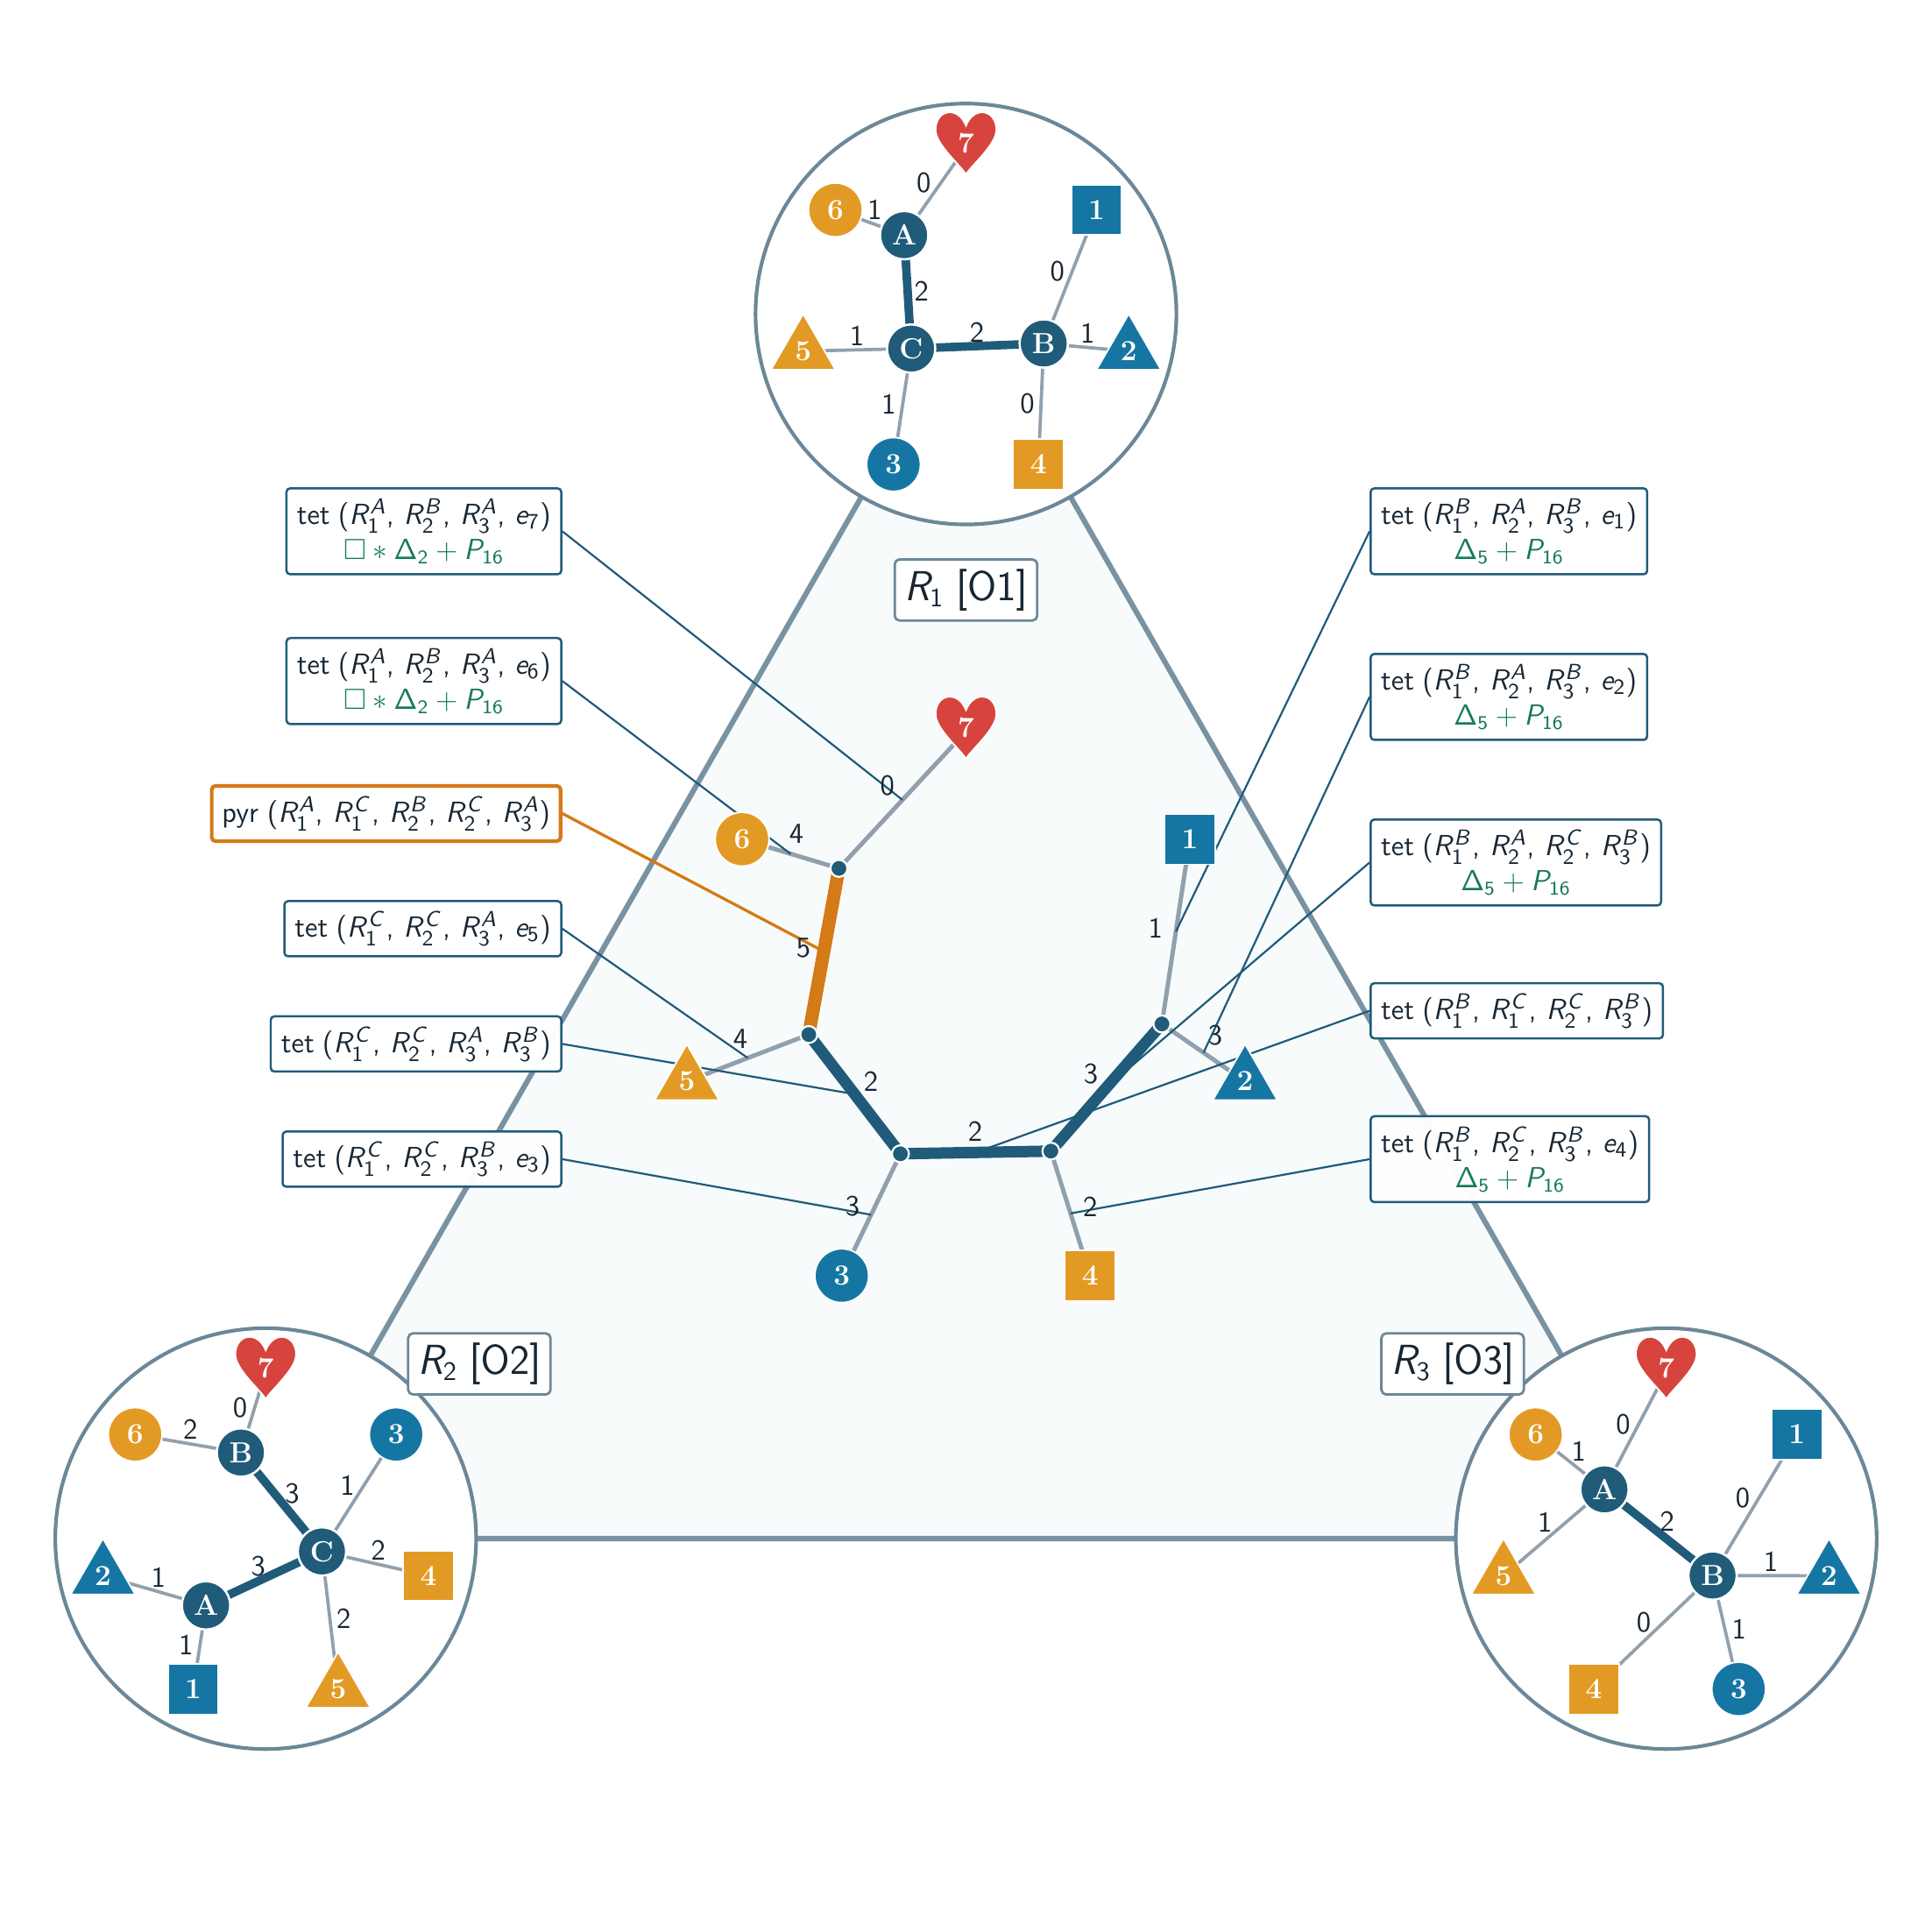
\begin{tikzpicture}[x=1cm,y=1cm]
\path[use as bounding box] (-13.65,-13.65) rectangle (13.65,13.65);
\path[support cell] (0.00000,9.45000)--(-10.15000,-8.30000)--(10.15000,-8.30000)--cycle;
\path[vertex disc] (0.00000,9.45000) circle[radius=3.05000cm];
\path[vertex disc] (-10.15000,-8.30000) circle[radius=3.05000cm];
\path[vertex disc] (10.15000,-8.30000) circle[radius=3.05000cm];
\coordinate (corner-1-v1) at (1.89203,10.95885);
\coordinate (corner-1-v2) at (2.35933,8.91150);
\coordinate (corner-1-v3) at (-1.05000,7.26966);
\coordinate (corner-1-v4) at (1.05000,7.26966);
\coordinate (corner-1-v5) at (-2.35933,8.91150);
\coordinate (corner-1-v6) at (-1.89203,10.95885);
\coordinate (corner-1-v7) at (0.00000,11.87000);
\coordinate (corner-1-v8) at (-0.89552,10.59262);
\coordinate (corner-1-v9) at (1.12671,9.02225);
\coordinate (corner-1-v10) at (-0.79454,8.94901);
\draw[internal edge] (corner-1-v8)--node[mini length,pos=0.5] {\(2\)}(corner-1-v10);
\draw[internal edge] (corner-1-v9)--node[mini length,pos=0.5] {\(2\)}(corner-1-v10);
\draw[pendant edge] (corner-1-v1)--node[mini length,pos=0.5] {\(0\)}(corner-1-v9);
\draw[pendant edge] (corner-1-v2)--node[mini length,pos=0.5] {\(1\)}(corner-1-v9);
\draw[pendant edge] (corner-1-v3)--node[mini length,pos=0.5] {\(1\)}(corner-1-v10);
\draw[pendant edge] (corner-1-v4)--node[mini length,pos=0.5] {\(0\)}(corner-1-v9);
\draw[pendant edge] (corner-1-v5)--node[mini length,pos=0.5] {\(1\)}(corner-1-v10);
\draw[pendant edge] (corner-1-v6)--node[mini length,pos=0.5] {\(1\)}(corner-1-v8);
\draw[pendant edge] (corner-1-v7)--node[mini length,pos=0.5] {\(0\)}(corner-1-v8);
\node[lettered vertex] at (corner-1-v8) {A};
\node[lettered vertex] at (corner-1-v9) {B};
\node[lettered vertex] at (corner-1-v10) {C};
\taxonone{corner-1-v1}
\taxontwo{corner-1-v2}
\taxonthree{corner-1-v3}
\taxonfour{corner-1-v4}
\taxonfive{corner-1-v5}
\taxonsix{corner-1-v6}
\taxonseven{corner-1-v7}
\node[ray title] at (0.00000,5.45000) {\(R_{1}\;[\mathrm{O}1]\)};
\coordinate (corner-2-v1) at (-11.20000,-10.48034);
\coordinate (corner-2-v2) at (-12.50933,-8.83850);
\coordinate (corner-2-v3) at (-8.25797,-6.79115);
\coordinate (corner-2-v4) at (-7.79067,-8.83850);
\coordinate (corner-2-v5) at (-9.10000,-10.48034);
\coordinate (corner-2-v6) at (-12.04203,-6.79115);
\coordinate (corner-2-v7) at (-10.15000,-5.88000);
\coordinate (corner-2-v8) at (-11.01458,-9.26833);
\coordinate (corner-2-v9) at (-10.50881,-7.05244);
\coordinate (corner-2-v10) at (-9.33441,-8.48615);
\draw[internal edge] (corner-2-v8)--node[mini length,pos=0.5] {\(3\)}(corner-2-v10);
\draw[internal edge] (corner-2-v9)--node[mini length,pos=0.5] {\(3\)}(corner-2-v10);
\draw[pendant edge] (corner-2-v1)--node[mini length,pos=0.5] {\(1\)}(corner-2-v8);
\draw[pendant edge] (corner-2-v2)--node[mini length,pos=0.5] {\(1\)}(corner-2-v8);
\draw[pendant edge] (corner-2-v3)--node[mini length,pos=0.5] {\(1\)}(corner-2-v10);
\draw[pendant edge] (corner-2-v4)--node[mini length,pos=0.5] {\(2\)}(corner-2-v10);
\draw[pendant edge] (corner-2-v5)--node[mini length,pos=0.5] {\(2\)}(corner-2-v10);
\draw[pendant edge] (corner-2-v6)--node[mini length,pos=0.5] {\(2\)}(corner-2-v9);
\draw[pendant edge] (corner-2-v7)--node[mini length,pos=0.5] {\(0\)}(corner-2-v9);
\node[lettered vertex] at (corner-2-v8) {A};
\node[lettered vertex] at (corner-2-v9) {B};
\node[lettered vertex] at (corner-2-v10) {C};
\taxonone{corner-2-v1}
\taxontwo{corner-2-v2}
\taxonthree{corner-2-v3}
\taxonfour{corner-2-v4}
\taxonfive{corner-2-v5}
\taxonsix{corner-2-v6}
\taxonseven{corner-2-v7}
\node[ray title] at (-7.05349,-5.76788) {\(R_{2}\;[\mathrm{O}2]\)};
\coordinate (corner-3-v1) at (12.04203,-6.79115);
\coordinate (corner-3-v2) at (12.50933,-8.83850);
\coordinate (corner-3-v3) at (11.20000,-10.48034);
\coordinate (corner-3-v4) at (9.10000,-10.48034);
\coordinate (corner-3-v5) at (7.79067,-8.83850);
\coordinate (corner-3-v6) at (8.25797,-6.79115);
\coordinate (corner-3-v7) at (10.15000,-5.88000);
\coordinate (corner-3-v8) at (9.25498,-7.58624);
\coordinate (corner-3-v9) at (10.82127,-8.83532);
\draw[internal edge] (corner-3-v8)--node[mini length,pos=0.5] {\(2\)}(corner-3-v9);
\draw[pendant edge] (corner-3-v1)--node[mini length,pos=0.5] {\(0\)}(corner-3-v9);
\draw[pendant edge] (corner-3-v2)--node[mini length,pos=0.5] {\(1\)}(corner-3-v9);
\draw[pendant edge] (corner-3-v3)--node[mini length,pos=0.5] {\(1\)}(corner-3-v9);
\draw[pendant edge] (corner-3-v4)--node[mini length,pos=0.5] {\(0\)}(corner-3-v9);
\draw[pendant edge] (corner-3-v5)--node[mini length,pos=0.5] {\(1\)}(corner-3-v8);
\draw[pendant edge] (corner-3-v6)--node[mini length,pos=0.5] {\(1\)}(corner-3-v8);
\draw[pendant edge] (corner-3-v7)--node[mini length,pos=0.5] {\(0\)}(corner-3-v8);
\node[lettered vertex] at (corner-3-v8) {A};
\node[lettered vertex] at (corner-3-v9) {B};
\taxonone{corner-3-v1}
\taxontwo{corner-3-v2}
\taxonthree{corner-3-v3}
\taxonfour{corner-3-v4}
\taxonfive{corner-3-v5}
\taxonsix{corner-3-v6}
\taxonseven{corner-3-v7}
\node[ray title] at (7.05349,-5.76788) {\(R_{3}\;[\mathrm{O}3]\)};
\coordinate (central-v1) at (3.24460,1.83748);
\coordinate (central-v2) at (4.04595,-1.67346);
\coordinate (central-v3) at (-1.80062,-4.48902);
\coordinate (central-v4) at (1.80062,-4.48902);
\coordinate (central-v5) at (-4.04595,-1.67346);
\coordinate (central-v6) at (-3.24460,1.83748);
\coordinate (central-v7) at (0.00000,3.40000);
\coordinate (central-v8) at (-1.84118,1.41461);
\coordinate (central-v9) at (2.84032,-0.83988);
\coordinate (central-v10) at (1.23040,-2.68367);
\coordinate (central-v11) at (-0.94972,-2.72212);
\coordinate (central-v12) at (-2.27895,-0.99366);
\draw[central pyramid edge] (central-v8)--(central-v12);
\draw[central internal edge] (central-v9)--(central-v10);
\draw[central internal edge] (central-v10)--(central-v11);
\draw[central internal edge] (central-v11)--(central-v12);
\draw[central pendant edge] (central-v1)--(central-v9);
\draw[central pendant edge] (central-v2)--(central-v9);
\draw[central pendant edge] (central-v3)--(central-v11);
\draw[central pendant edge] (central-v4)--(central-v10);
\draw[central pendant edge] (central-v5)--(central-v12);
\draw[central pendant edge] (central-v6)--(central-v8);
\draw[central pendant edge] (central-v7)--(central-v8);
\draw[edge leader] (-5.85000,6.30000)--(-0.92059,2.40730);
\draw[edge leader] (-5.85000,4.13000)--(-2.54289,1.62605);
\draw[pyramid leader] (-5.85000,2.21000)--(-2.06007,0.21048);
\draw[edge leader] (-5.85000,0.54000)--(-3.16245,-1.33356);
\draw[edge leader] (-5.85000,-1.13000)--(-1.61434,-1.85789);
\draw[edge leader] (-5.85000,-2.80000)--(-1.37517,-3.60557);
\draw[edge leader] (5.85000,6.30000)--(3.04246,0.49880);
\draw[edge leader] (5.85000,3.90000)--(3.44313,-1.25667);
\draw[edge leader] (5.85000,1.50000)--(2.03536,-1.76178);
\draw[edge leader] (5.85000,-0.65000)--(0.14034,-2.70290);
\draw[edge leader] (5.85000,-2.80000)--(1.51551,-3.58635);
\node[internal vertex] at (central-v8) {};
\node[internal vertex] at (central-v9) {};
\node[internal vertex] at (central-v10) {};
\node[internal vertex] at (central-v11) {};
\node[internal vertex] at (central-v12) {};
\taxonone{central-v1}
\taxontwo{central-v2}
\taxonthree{central-v3}
\taxonfour{central-v4}
\taxonfive{central-v5}
\taxonsix{central-v6}
\taxonseven{central-v7}
\path (central-v8)--node[central length,pos=.50] {\(5\)}(central-v12);
\path (central-v9)--node[central length,pos=.50] {\(3\)}(central-v10);
\path (central-v10)--node[central length,pos=.50] {\(2\)}(central-v11);
\path (central-v11)--node[central length,pos=.50] {\(2\)}(central-v12);
\path (central-v1)--node[central length,pos=.50] {\(1\)}(central-v9);
\path (central-v2)--node[central length,pos=.50] {\(3\)}(central-v9);
\path (central-v3)--node[central length,pos=.50] {\(3\)}(central-v11);
\path (central-v4)--node[central length,pos=.50] {\(2\)}(central-v10);
\path (central-v5)--node[central length,pos=.50] {\(4\)}(central-v12);
\path (central-v6)--node[central length,pos=.50] {\(4\)}(central-v8);
\path (central-v7)--node[central length,pos=.50] {\(0\)}(central-v8);
\node[edge callout,anchor=east] (callout-1) at (-5.85000,6.30000) {\(\mathrm{tet}\;(R_{1}^{A},\,R_{2}^{B},\,R_{3}^{A},\,e_{7})\)\\{\fontsize{12}{14}\selectfont\color{toricgreen}\(\square\ast\Delta_{2}+P_{16}\)}};
\node[edge callout,anchor=east] (callout-2) at (-5.85000,4.13000) {\(\mathrm{tet}\;(R_{1}^{A},\,R_{2}^{B},\,R_{3}^{A},\,e_{6})\)\\{\fontsize{12}{14}\selectfont\color{toricgreen}\(\square\ast\Delta_{2}+P_{16}\)}};
\node[pyramid callout,anchor=east] (callout-3) at (-5.85000,2.21000) {\(\mathrm{pyr}\;(R_{1}^{A},\,R_{1}^{C},\,R_{2}^{B},\,R_{2}^{C},\,R_{3}^{A})\)};
\node[edge callout,anchor=east] (callout-4) at (-5.85000,0.54000) {\(\mathrm{tet}\;(R_{1}^{C},\,R_{2}^{C},\,R_{3}^{A},\,e_{5})\)};
\node[edge callout,anchor=east] (callout-5) at (-5.85000,-1.13000) {\(\mathrm{tet}\;(R_{1}^{C},\,R_{2}^{C},\,R_{3}^{A},\,R_{3}^{B})\)};
\node[edge callout,anchor=east] (callout-6) at (-5.85000,-2.80000) {\(\mathrm{tet}\;(R_{1}^{C},\,R_{2}^{C},\,R_{3}^{B},\,e_{3})\)};
\node[edge callout,anchor=west] (callout-7) at (5.85000,6.30000) {\(\mathrm{tet}\;(R_{1}^{B},\,R_{2}^{A},\,R_{3}^{B},\,e_{1})\)\\{\fontsize{12}{14}\selectfont\color{toricgreen}\(\Delta_{5}+P_{16}\)}};
\node[edge callout,anchor=west] (callout-8) at (5.85000,3.90000) {\(\mathrm{tet}\;(R_{1}^{B},\,R_{2}^{A},\,R_{3}^{B},\,e_{2})\)\\{\fontsize{12}{14}\selectfont\color{toricgreen}\(\Delta_{5}+P_{16}\)}};
\node[edge callout,anchor=west] (callout-9) at (5.85000,1.50000) {\(\mathrm{tet}\;(R_{1}^{B},\,R_{2}^{A},\,R_{2}^{C},\,R_{3}^{B})\)\\{\fontsize{12}{14}\selectfont\color{toricgreen}\(\Delta_{5}+P_{16}\)}};
\node[edge callout,anchor=west] (callout-10) at (5.85000,-0.65000) {\(\mathrm{tet}\;(R_{1}^{B},\,R_{1}^{C},\,R_{2}^{C},\,R_{3}^{B})\)};
\node[edge callout,anchor=west] (callout-11) at (5.85000,-2.80000) {\(\mathrm{tet}\;(R_{1}^{B},\,R_{2}^{C},\,R_{3}^{B},\,e_{4})\)\\{\fontsize{12}{14}\selectfont\color{toricgreen}\(\Delta_{5}+P_{16}\)}};
\end{tikzpicture}\end{center}\vspace{-1mm}
\begin{atlasbox}\begin{atlaspanel}
\textcolor{toricgreen}{\bfseries PRIME TORIC}\quad \(P_{16}\):\enspace \(\mathrm{U}^{4}_{8,8}\ast\Delta_{0}\)\quad \(f=(9,27,38,27,9)\)\quad 14 lattice points\quad \(f(\mathrm{U}^{4}_{8,8})=(8,19,19,8)\)
\end{atlaspanel}\end{atlasbox}
\clearpage
\begin{atlaspanel}[top=1mm,bottom=2mm]
\AtlasSupportOrbitSplit{%
\vspace*{-3mm}\mbox{{\LARGE\bfseries Triangle orbit 17}\hspace{3mm}\raisebox{.8mm}[0pt][0pt]{{\fontsize{16}{18}\selectfont\color{muted}size 12}}}%
}{%
\vspace*{-3mm}{\fontsize{13}{16}\selectfont{\color{muted}\(\mathbb{Q}\) and \(\mathbb{F}_2\)}\quad{\color{muted}\(\underline{\{2,\,3,\,15\}}\), \(\{2,\,5,\,15\}\), \(\{3,\,15,\,25\}\), \(\{5,\,15,\,26\}\), \(\{15,\,25,\,27\}\), \(\{15,\,26,\,27\}\), \(\{16,\,29,\,32\}\), \(\{16,\,29,\,31\}\), \(\{28,\,29,\,46\}\), \(\{28,\,29,\,47\}\), \(\{29,\,31,\,46\}\), \(\{29,\,32,\,47\}\)}\rule[-3mm]{0pt}{3mm}}%
}%
\end{atlaspanel}\vspace{2mm}
\begin{center}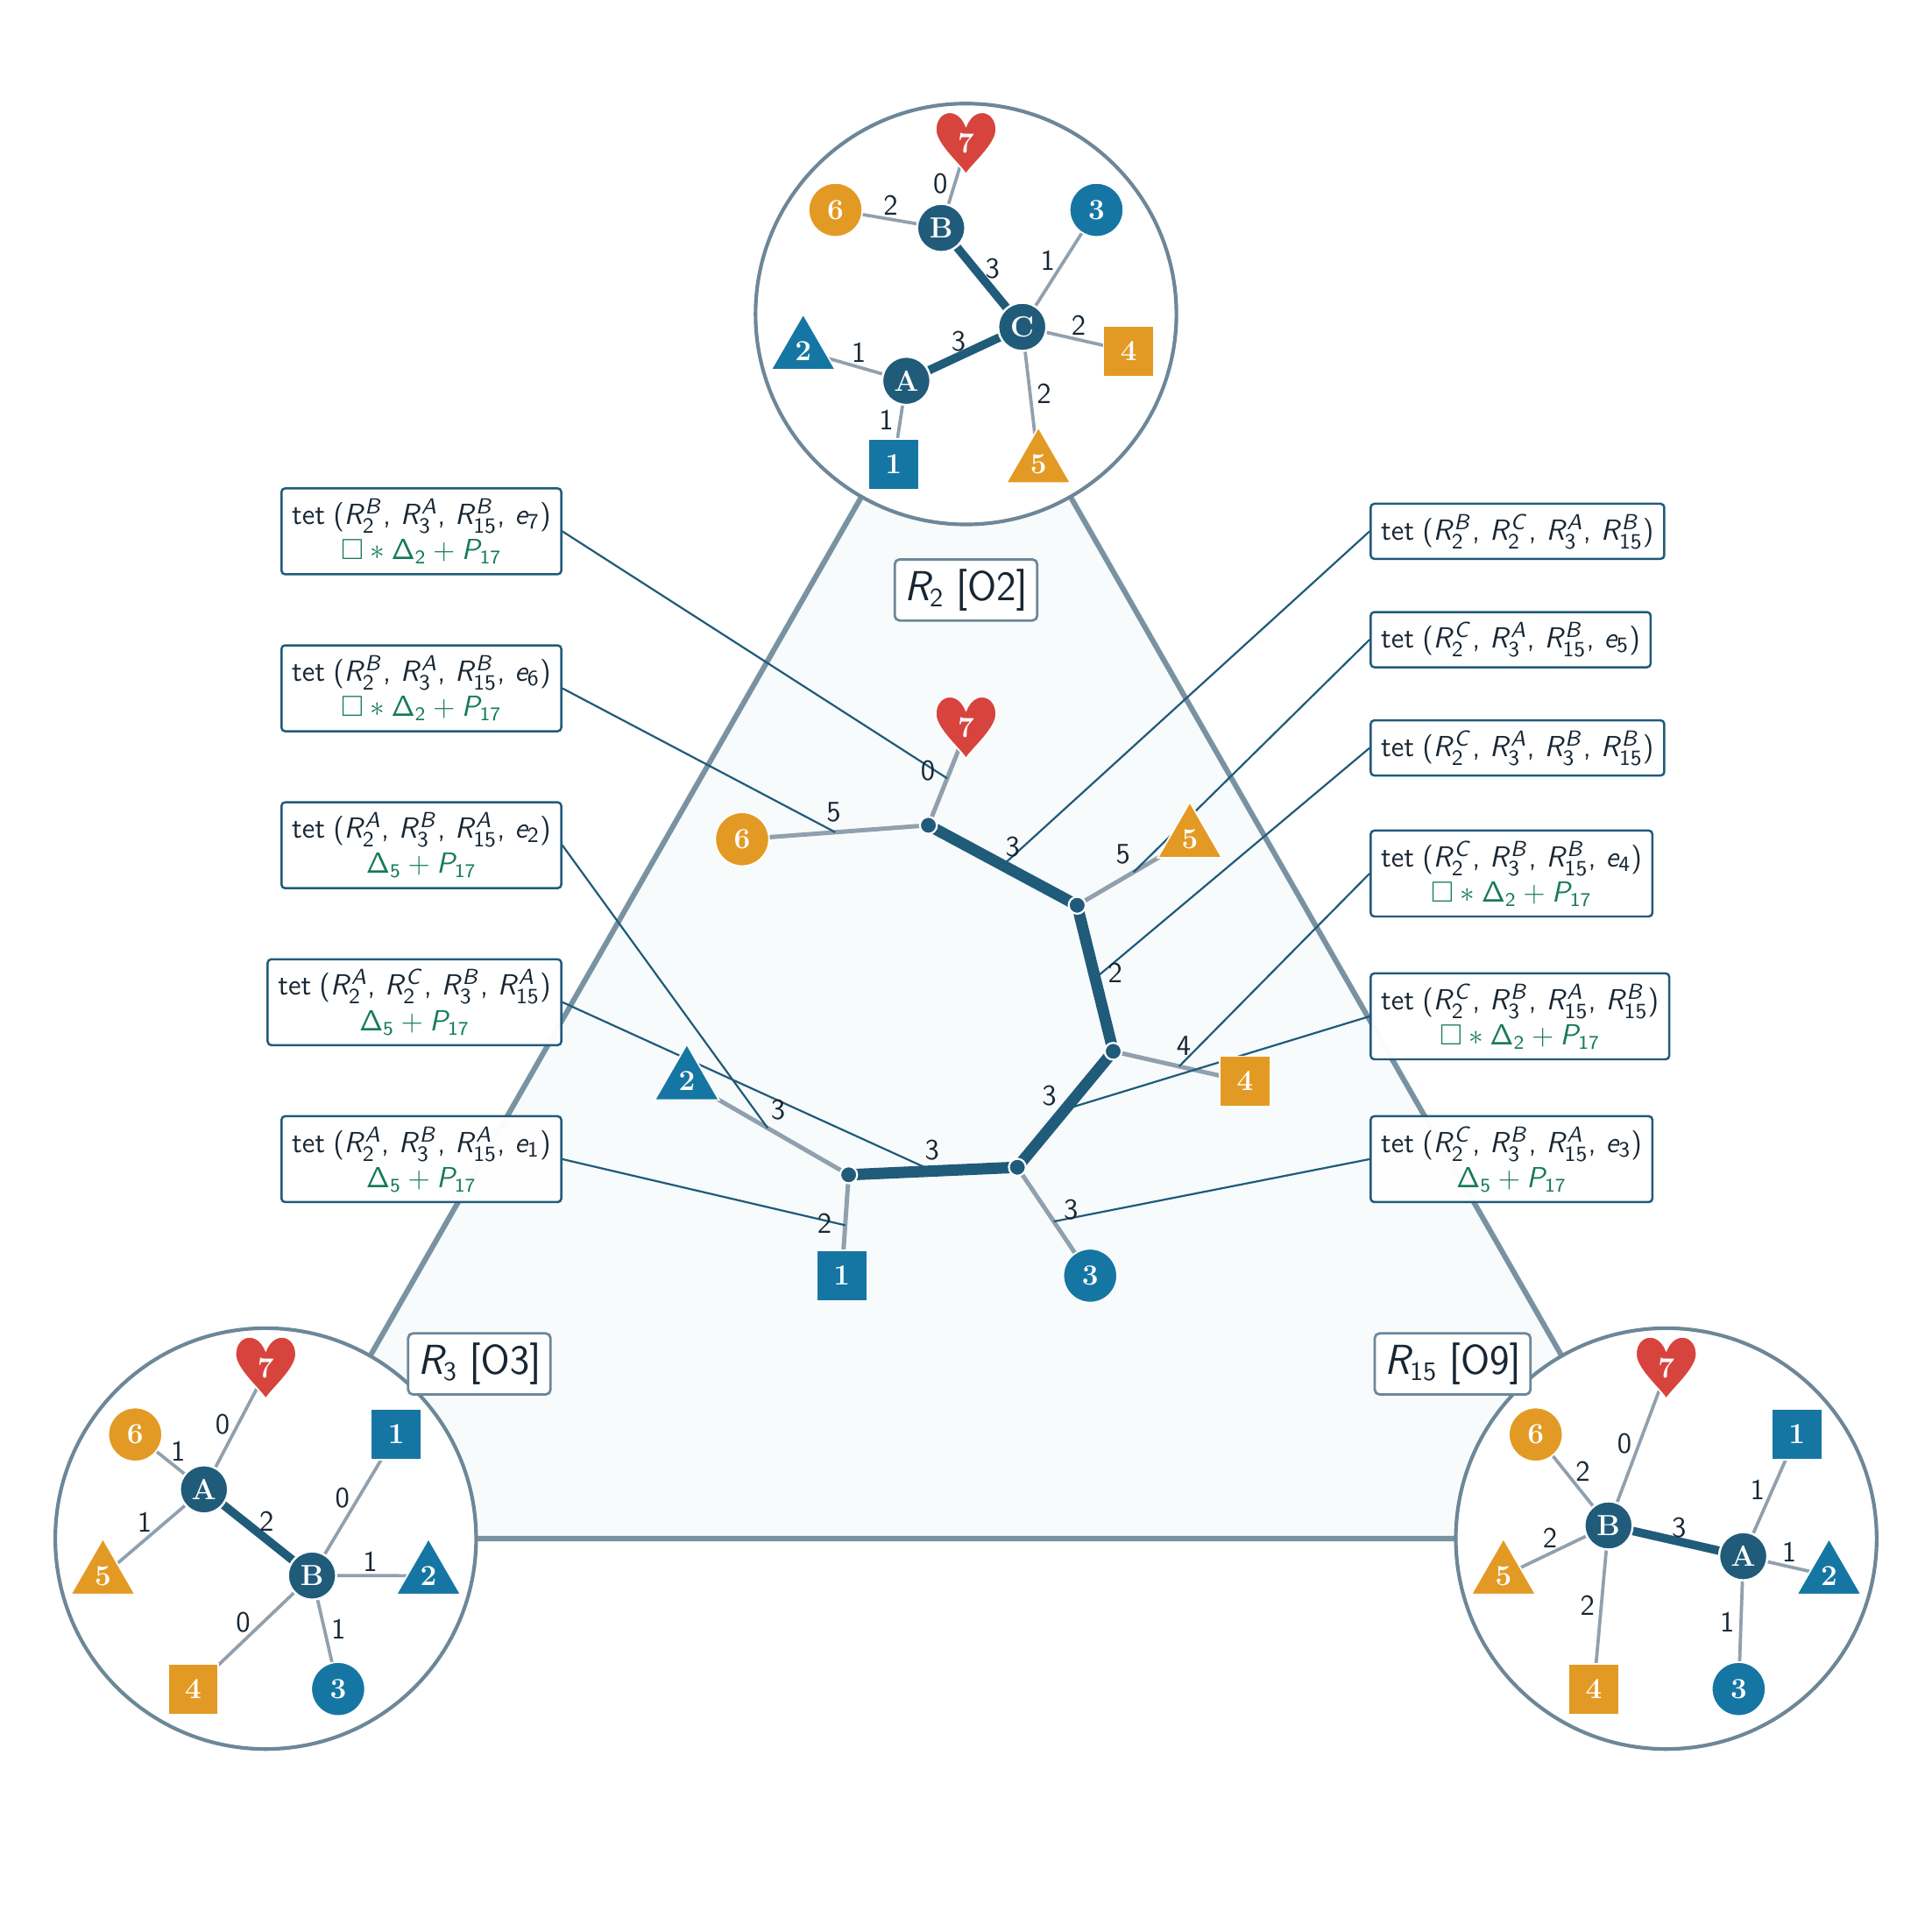
\begin{tikzpicture}[x=1cm,y=1cm]
\path[use as bounding box] (-13.65,-13.65) rectangle (13.65,13.65);
\path[support cell] (0.00000,9.45000)--(-10.15000,-8.30000)--(10.15000,-8.30000)--cycle;
\path[vertex disc] (0.00000,9.45000) circle[radius=3.05000cm];
\path[vertex disc] (-10.15000,-8.30000) circle[radius=3.05000cm];
\path[vertex disc] (10.15000,-8.30000) circle[radius=3.05000cm];
\coordinate (corner-1-v1) at (-1.05000,7.26966);
\coordinate (corner-1-v2) at (-2.35933,8.91150);
\coordinate (corner-1-v3) at (1.89203,10.95885);
\coordinate (corner-1-v4) at (2.35933,8.91150);
\coordinate (corner-1-v5) at (1.05000,7.26966);
\coordinate (corner-1-v6) at (-1.89203,10.95885);
\coordinate (corner-1-v7) at (0.00000,11.87000);
\coordinate (corner-1-v8) at (-0.86458,8.48167);
\coordinate (corner-1-v9) at (-0.35881,10.69756);
\coordinate (corner-1-v10) at (0.81559,9.26385);
\draw[internal edge] (corner-1-v8)--node[mini length,pos=0.5] {\(3\)}(corner-1-v10);
\draw[internal edge] (corner-1-v9)--node[mini length,pos=0.5] {\(3\)}(corner-1-v10);
\draw[pendant edge] (corner-1-v1)--node[mini length,pos=0.5] {\(1\)}(corner-1-v8);
\draw[pendant edge] (corner-1-v2)--node[mini length,pos=0.5] {\(1\)}(corner-1-v8);
\draw[pendant edge] (corner-1-v3)--node[mini length,pos=0.5] {\(1\)}(corner-1-v10);
\draw[pendant edge] (corner-1-v4)--node[mini length,pos=0.5] {\(2\)}(corner-1-v10);
\draw[pendant edge] (corner-1-v5)--node[mini length,pos=0.5] {\(2\)}(corner-1-v10);
\draw[pendant edge] (corner-1-v6)--node[mini length,pos=0.5] {\(2\)}(corner-1-v9);
\draw[pendant edge] (corner-1-v7)--node[mini length,pos=0.5] {\(0\)}(corner-1-v9);
\node[lettered vertex] at (corner-1-v8) {A};
\node[lettered vertex] at (corner-1-v9) {B};
\node[lettered vertex] at (corner-1-v10) {C};
\taxonone{corner-1-v1}
\taxontwo{corner-1-v2}
\taxonthree{corner-1-v3}
\taxonfour{corner-1-v4}
\taxonfive{corner-1-v5}
\taxonsix{corner-1-v6}
\taxonseven{corner-1-v7}
\node[ray title] at (0.00000,5.45000) {\(R_{2}\;[\mathrm{O}2]\)};
\coordinate (corner-2-v1) at (-8.25797,-6.79115);
\coordinate (corner-2-v2) at (-7.79067,-8.83850);
\coordinate (corner-2-v3) at (-9.10000,-10.48034);
\coordinate (corner-2-v4) at (-11.20000,-10.48034);
\coordinate (corner-2-v5) at (-12.50933,-8.83850);
\coordinate (corner-2-v6) at (-12.04203,-6.79115);
\coordinate (corner-2-v7) at (-10.15000,-5.88000);
\coordinate (corner-2-v8) at (-11.04502,-7.58624);
\coordinate (corner-2-v9) at (-9.47873,-8.83532);
\draw[internal edge] (corner-2-v8)--node[mini length,pos=0.5] {\(2\)}(corner-2-v9);
\draw[pendant edge] (corner-2-v1)--node[mini length,pos=0.5] {\(0\)}(corner-2-v9);
\draw[pendant edge] (corner-2-v2)--node[mini length,pos=0.5] {\(1\)}(corner-2-v9);
\draw[pendant edge] (corner-2-v3)--node[mini length,pos=0.5] {\(1\)}(corner-2-v9);
\draw[pendant edge] (corner-2-v4)--node[mini length,pos=0.5] {\(0\)}(corner-2-v9);
\draw[pendant edge] (corner-2-v5)--node[mini length,pos=0.5] {\(1\)}(corner-2-v8);
\draw[pendant edge] (corner-2-v6)--node[mini length,pos=0.5] {\(1\)}(corner-2-v8);
\draw[pendant edge] (corner-2-v7)--node[mini length,pos=0.5] {\(0\)}(corner-2-v8);
\node[lettered vertex] at (corner-2-v8) {A};
\node[lettered vertex] at (corner-2-v9) {B};
\taxonone{corner-2-v1}
\taxontwo{corner-2-v2}
\taxonthree{corner-2-v3}
\taxonfour{corner-2-v4}
\taxonfive{corner-2-v5}
\taxonsix{corner-2-v6}
\taxonseven{corner-2-v7}
\node[ray title] at (-7.05349,-5.76788) {\(R_{3}\;[\mathrm{O}3]\)};
\coordinate (corner-3-v1) at (12.04203,-6.79115);
\coordinate (corner-3-v2) at (12.50933,-8.83850);
\coordinate (corner-3-v3) at (11.20000,-10.48034);
\coordinate (corner-3-v4) at (9.10000,-10.48034);
\coordinate (corner-3-v5) at (7.79067,-8.83850);
\coordinate (corner-3-v6) at (8.25797,-6.79115);
\coordinate (corner-3-v7) at (10.15000,-5.88000);
\coordinate (corner-3-v8) at (11.26608,-8.55474);
\coordinate (corner-3-v9) at (9.31294,-8.10895);
\draw[internal edge] (corner-3-v8)--node[mini length,pos=0.5] {\(3\)}(corner-3-v9);
\draw[pendant edge] (corner-3-v1)--node[mini length,pos=0.5] {\(1\)}(corner-3-v8);
\draw[pendant edge] (corner-3-v2)--node[mini length,pos=0.5] {\(1\)}(corner-3-v8);
\draw[pendant edge] (corner-3-v3)--node[mini length,pos=0.5] {\(1\)}(corner-3-v8);
\draw[pendant edge] (corner-3-v4)--node[mini length,pos=0.5] {\(2\)}(corner-3-v9);
\draw[pendant edge] (corner-3-v5)--node[mini length,pos=0.5] {\(2\)}(corner-3-v9);
\draw[pendant edge] (corner-3-v6)--node[mini length,pos=0.5] {\(2\)}(corner-3-v9);
\draw[pendant edge] (corner-3-v7)--node[mini length,pos=0.5] {\(0\)}(corner-3-v9);
\node[lettered vertex] at (corner-3-v8) {A};
\node[lettered vertex] at (corner-3-v9) {B};
\taxonone{corner-3-v1}
\taxontwo{corner-3-v2}
\taxonthree{corner-3-v3}
\taxonfour{corner-3-v4}
\taxonfive{corner-3-v5}
\taxonsix{corner-3-v6}
\taxonseven{corner-3-v7}
\node[ray title] at (7.05349,-5.76788) {\(R_{15}\;[\mathrm{O}9]\)};
\coordinate (central-v1) at (-1.80062,-4.48902);
\coordinate (central-v2) at (-4.04595,-1.67346);
\coordinate (central-v3) at (1.80062,-4.48902);
\coordinate (central-v4) at (4.04595,-1.67346);
\coordinate (central-v5) at (3.24460,1.83748);
\coordinate (central-v6) at (-3.24460,1.83748);
\coordinate (central-v7) at (0.00000,3.40000);
\coordinate (central-v8) at (-1.70064,-3.02669);
\coordinate (central-v9) at (0.74466,-2.91760);
\coordinate (central-v10) at (-0.54440,2.03911);
\coordinate (central-v11) at (2.13401,-1.23707);
\coordinate (central-v12) at (1.61140,0.87984);
\draw[central internal edge] (central-v8)--(central-v9);
\draw[central internal edge] (central-v9)--(central-v11);
\draw[central internal edge] (central-v10)--(central-v12);
\draw[central internal edge] (central-v11)--(central-v12);
\draw[central pendant edge] (central-v1)--(central-v8);
\draw[central pendant edge] (central-v2)--(central-v8);
\draw[central pendant edge] (central-v3)--(central-v9);
\draw[central pendant edge] (central-v4)--(central-v11);
\draw[central pendant edge] (central-v5)--(central-v12);
\draw[central pendant edge] (central-v6)--(central-v10);
\draw[central pendant edge] (central-v7)--(central-v10);
\draw[edge leader] (-5.85000,6.30000)--(-0.27220,2.71955);
\draw[edge leader] (-5.85000,4.02500)--(-1.89450,1.93829);
\draw[edge leader] (-5.85000,1.75000)--(-2.87329,-2.35008);
\draw[edge leader] (-5.85000,-0.52500)--(-0.47799,-2.97214);
\draw[edge leader] (-5.85000,-2.80000)--(-1.75063,-3.75786);
\draw[edge leader] (5.85000,6.30000)--(0.53350,1.45947);
\draw[edge leader] (5.85000,4.73000)--(2.42800,1.35866);
\draw[edge leader] (5.85000,3.16000)--(1.87270,-0.17862);
\draw[edge leader] (5.85000,1.34000)--(3.08998,-1.45527);
\draw[edge leader] (5.85000,-0.73000)--(1.43933,-2.07733);
\draw[edge leader] (5.85000,-2.80000)--(1.27264,-3.70331);
\node[internal vertex] at (central-v8) {};
\node[internal vertex] at (central-v9) {};
\node[internal vertex] at (central-v10) {};
\node[internal vertex] at (central-v11) {};
\node[internal vertex] at (central-v12) {};
\taxonone{central-v1}
\taxontwo{central-v2}
\taxonthree{central-v3}
\taxonfour{central-v4}
\taxonfive{central-v5}
\taxonsix{central-v6}
\taxonseven{central-v7}
\path (central-v8)--node[central length,pos=.50] {\(3\)}(central-v9);
\path (central-v9)--node[central length,pos=.50] {\(3\)}(central-v11);
\path (central-v10)--node[central length,pos=.50] {\(3\)}(central-v12);
\path (central-v11)--node[central length,pos=.50] {\(2\)}(central-v12);
\path (central-v1)--node[central length,pos=.50] {\(2\)}(central-v8);
\path (central-v2)--node[central length,pos=.50] {\(3\)}(central-v8);
\path (central-v3)--node[central length,pos=.50] {\(3\)}(central-v9);
\path (central-v4)--node[central length,pos=.50] {\(4\)}(central-v11);
\path (central-v5)--node[central length,pos=.50] {\(5\)}(central-v12);
\path (central-v6)--node[central length,pos=.50] {\(5\)}(central-v10);
\path (central-v7)--node[central length,pos=.50] {\(0\)}(central-v10);
\node[edge callout,anchor=east] (callout-1) at (-5.85000,6.30000) {\(\mathrm{tet}\;(R_{2}^{B},\,R_{3}^{A},\,R_{15}^{B},\,e_{7})\)\\{\fontsize{12}{14}\selectfont\color{toricgreen}\(\square\ast\Delta_{2}+P_{17}\)}};
\node[edge callout,anchor=east] (callout-2) at (-5.85000,4.02500) {\(\mathrm{tet}\;(R_{2}^{B},\,R_{3}^{A},\,R_{15}^{B},\,e_{6})\)\\{\fontsize{12}{14}\selectfont\color{toricgreen}\(\square\ast\Delta_{2}+P_{17}\)}};
\node[edge callout,anchor=east] (callout-3) at (-5.85000,1.75000) {\(\mathrm{tet}\;(R_{2}^{A},\,R_{3}^{B},\,R_{15}^{A},\,e_{2})\)\\{\fontsize{12}{14}\selectfont\color{toricgreen}\(\Delta_{5}+P_{17}\)}};
\node[edge callout,anchor=east] (callout-4) at (-5.85000,-0.52500) {\(\mathrm{tet}\;(R_{2}^{A},\,R_{2}^{C},\,R_{3}^{B},\,R_{15}^{A})\)\\{\fontsize{12}{14}\selectfont\color{toricgreen}\(\Delta_{5}+P_{17}\)}};
\node[edge callout,anchor=east] (callout-5) at (-5.85000,-2.80000) {\(\mathrm{tet}\;(R_{2}^{A},\,R_{3}^{B},\,R_{15}^{A},\,e_{1})\)\\{\fontsize{12}{14}\selectfont\color{toricgreen}\(\Delta_{5}+P_{17}\)}};
\node[edge callout,anchor=west] (callout-6) at (5.85000,6.30000) {\(\mathrm{tet}\;(R_{2}^{B},\,R_{2}^{C},\,R_{3}^{A},\,R_{15}^{B})\)};
\node[edge callout,anchor=west] (callout-7) at (5.85000,4.73000) {\(\mathrm{tet}\;(R_{2}^{C},\,R_{3}^{A},\,R_{15}^{B},\,e_{5})\)};
\node[edge callout,anchor=west] (callout-8) at (5.85000,3.16000) {\(\mathrm{tet}\;(R_{2}^{C},\,R_{3}^{A},\,R_{3}^{B},\,R_{15}^{B})\)};
\node[edge callout,anchor=west] (callout-9) at (5.85000,1.34000) {\(\mathrm{tet}\;(R_{2}^{C},\,R_{3}^{B},\,R_{15}^{B},\,e_{4})\)\\{\fontsize{12}{14}\selectfont\color{toricgreen}\(\square\ast\Delta_{2}+P_{17}\)}};
\node[edge callout,anchor=west] (callout-10) at (5.85000,-0.73000) {\(\mathrm{tet}\;(R_{2}^{C},\,R_{3}^{B},\,R_{15}^{A},\,R_{15}^{B})\)\\{\fontsize{12}{14}\selectfont\color{toricgreen}\(\square\ast\Delta_{2}+P_{17}\)}};
\node[edge callout,anchor=west] (callout-11) at (5.85000,-2.80000) {\(\mathrm{tet}\;(R_{2}^{C},\,R_{3}^{B},\,R_{15}^{A},\,e_{3})\)\\{\fontsize{12}{14}\selectfont\color{toricgreen}\(\Delta_{5}+P_{17}\)}};
\end{tikzpicture}\end{center}\vspace{-1mm}
\begin{atlasbox}\begin{atlaspanel}
\textcolor{toricgreen}{\bfseries PRIME TORIC}\quad \(P_{17}\):\enspace \(\mathrm{U}^{4}_{9,8}\ast\Delta_{0}\)\quad \(f=(10,30,41,28,9)\)\quad 14 lattice points\quad \(f(\mathrm{U}^{4}_{9,8})=(9,21,20,8)\)
\end{atlaspanel}\end{atlasbox}
\clearpage
\begin{atlaspanel}[top=1mm,bottom=2mm]
\AtlasSupportOrbitSplit{%
\vspace*{-3mm}\mbox{{\LARGE\bfseries Triangle orbit 18}\hspace{3mm}\raisebox{.8mm}[0pt][0pt]{{\fontsize{16}{18}\selectfont\color{muted}size 6}}}%
}{%
\vspace*{-3mm}{\fontsize{13}{16}\selectfont{\color{animalblue}\bfseries\(\mathbb{F}_2\) only}\quad{\color{muted}\(\underline{\{9,\,40,\,52\}}\), \(\{6,\,9,\,52\}\), \(\{12,\,30,\,53\}\), \(\{11,\,30,\,53\}\), \(\{10,\,41,\,54\}\), \(\{7,\,10,\,54\}\)}\rule[-3mm]{0pt}{3mm}}%
}%
\end{atlaspanel}\vspace{2mm}
\begin{center}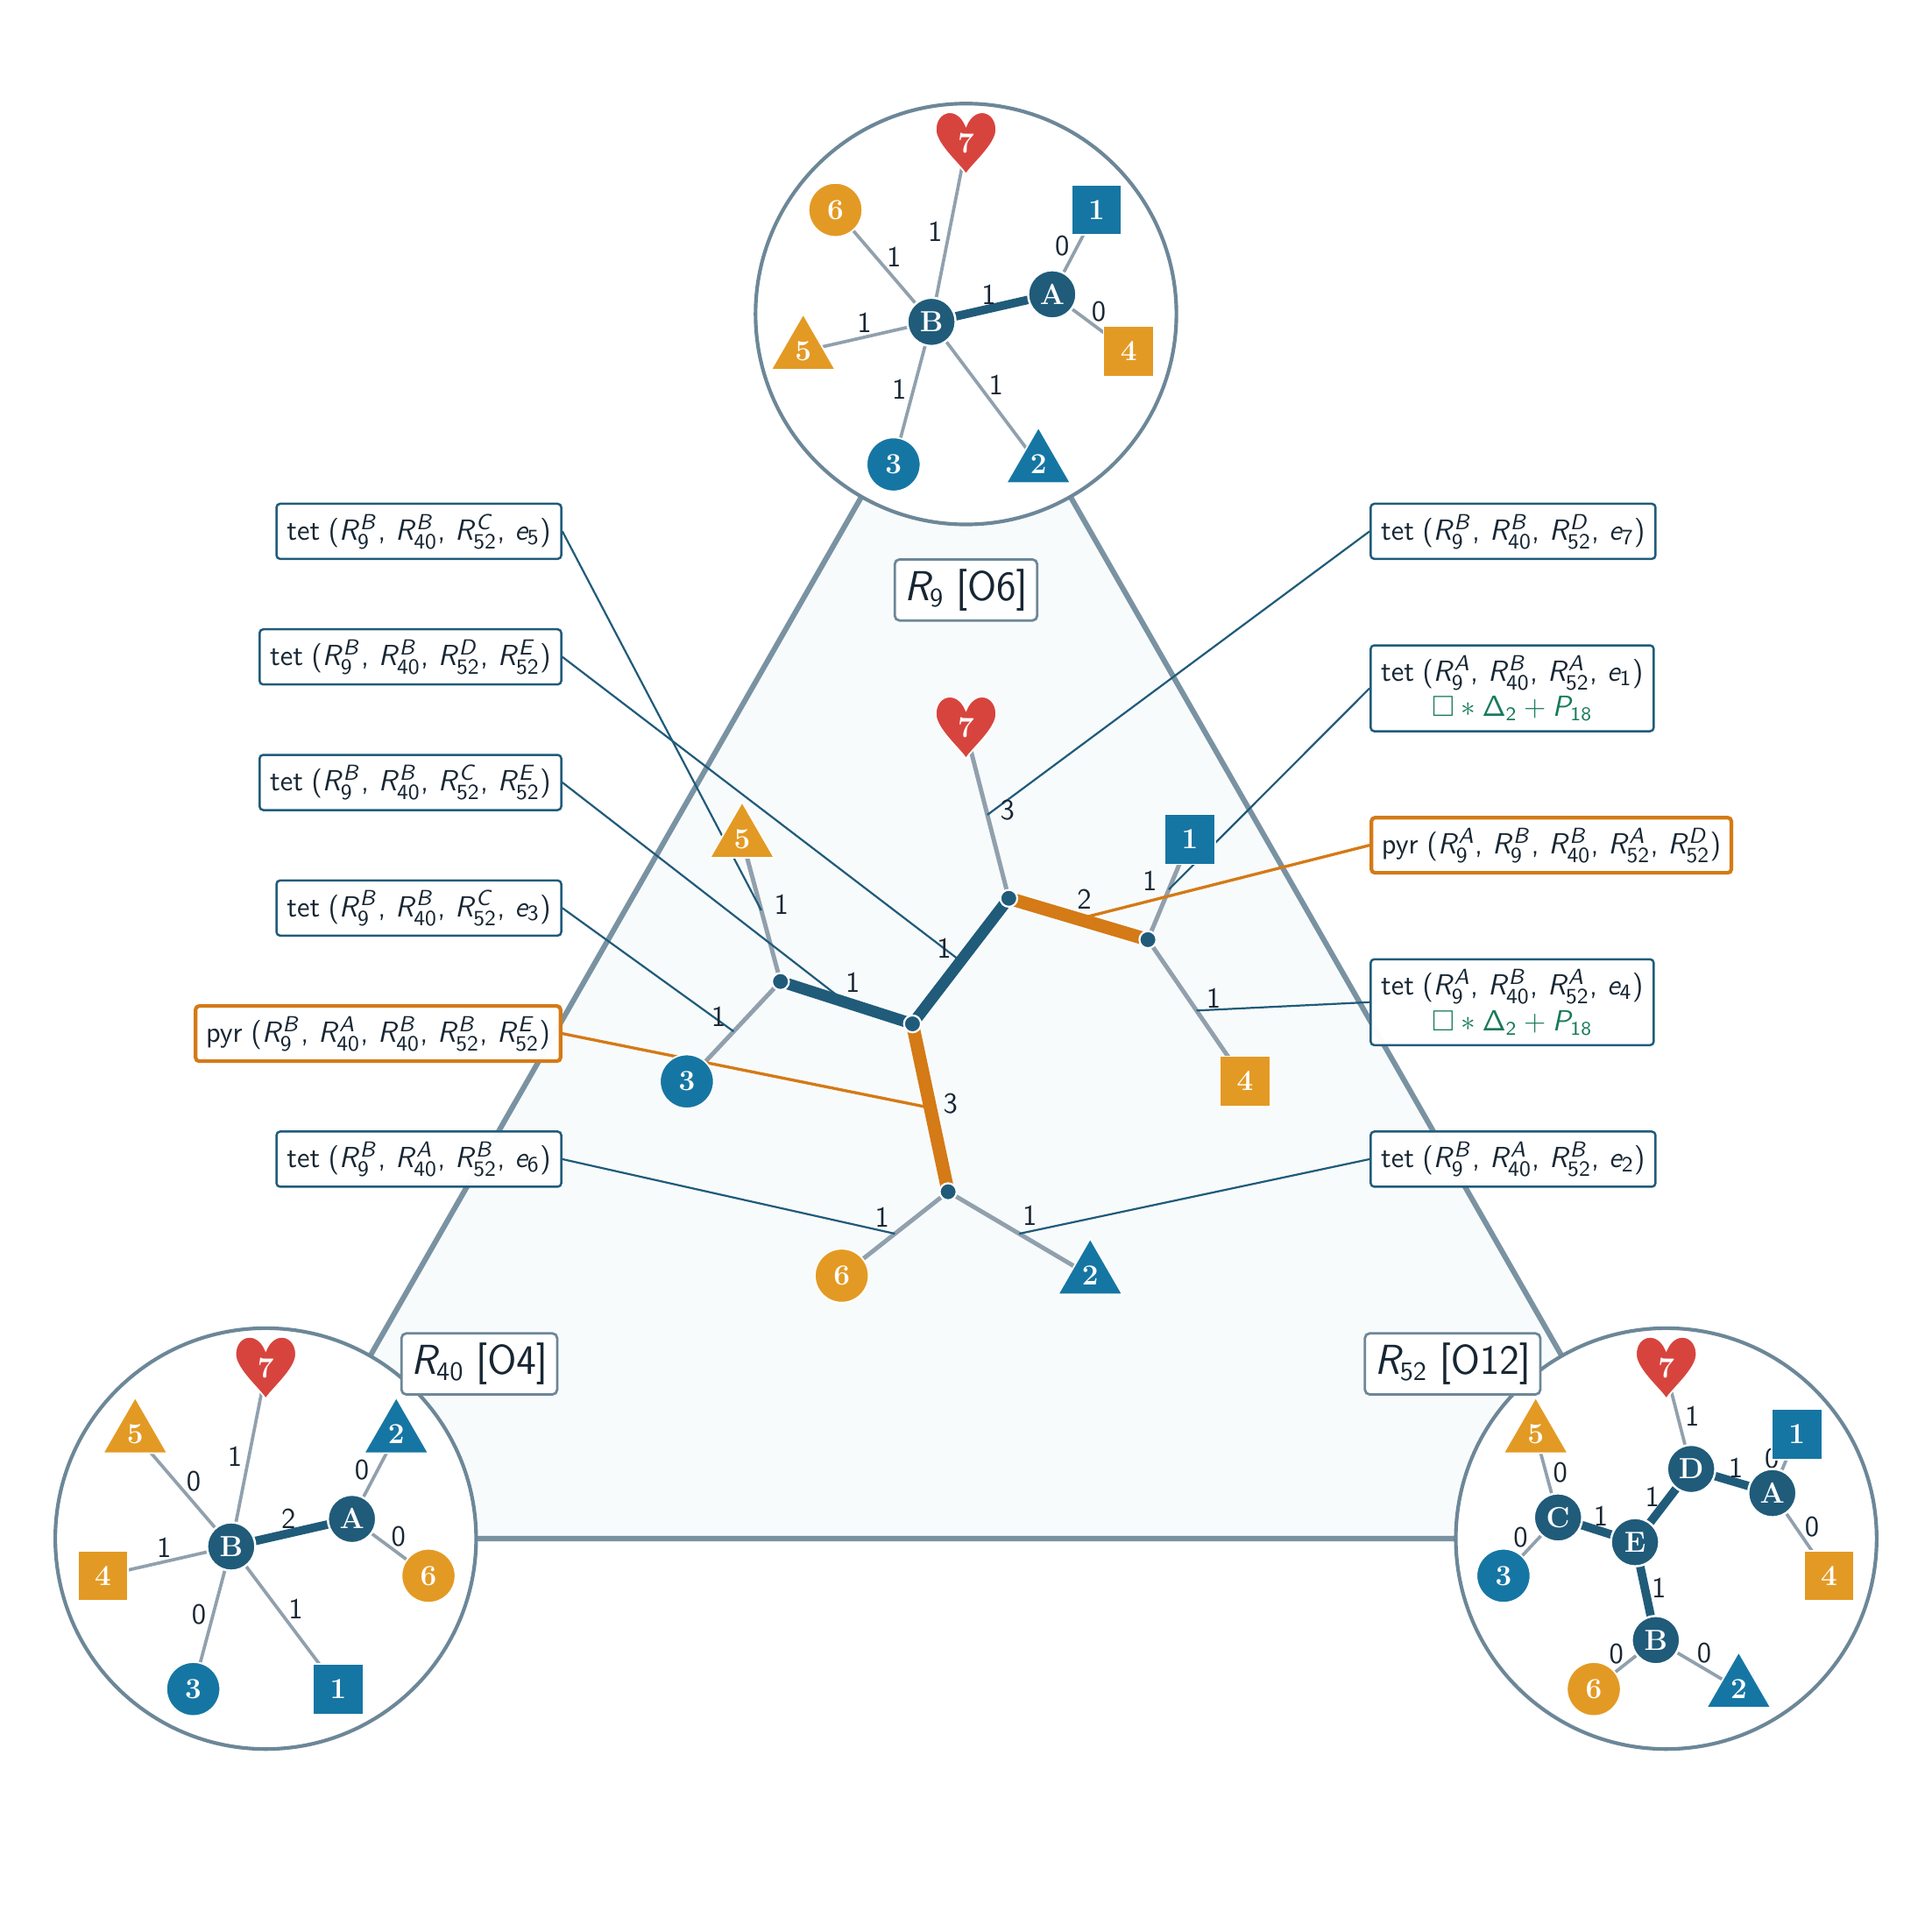
\begin{tikzpicture}[x=1cm,y=1cm]
\path[use as bounding box] (-13.65,-13.65) rectangle (13.65,13.65);
\path[support cell] (0.00000,9.45000)--(-10.15000,-8.30000)--(10.15000,-8.30000)--cycle;
\path[vertex disc] (0.00000,9.45000) circle[radius=3.05000cm];
\path[vertex disc] (-10.15000,-8.30000) circle[radius=3.05000cm];
\path[vertex disc] (10.15000,-8.30000) circle[radius=3.05000cm];
\coordinate (corner-1-v1) at (1.89203,10.95885);
\coordinate (corner-1-v2) at (1.05000,7.26966);
\coordinate (corner-1-v3) at (-1.05000,7.26966);
\coordinate (corner-1-v4) at (2.35933,8.91150);
\coordinate (corner-1-v5) at (-2.35933,8.91150);
\coordinate (corner-1-v6) at (-1.89203,10.95885);
\coordinate (corner-1-v7) at (0.00000,11.87000);
\coordinate (corner-1-v8) at (1.25040,9.73540);
\coordinate (corner-1-v9) at (-0.50016,9.33584);
\draw[internal edge] (corner-1-v8)--node[mini length,pos=0.5] {\(1\)}(corner-1-v9);
\draw[pendant edge] (corner-1-v1)--node[mini length,pos=0.5] {\(0\)}(corner-1-v8);
\draw[pendant edge] (corner-1-v2)--node[mini length,pos=0.5] {\(1\)}(corner-1-v9);
\draw[pendant edge] (corner-1-v3)--node[mini length,pos=0.5] {\(1\)}(corner-1-v9);
\draw[pendant edge] (corner-1-v4)--node[mini length,pos=0.5] {\(0\)}(corner-1-v8);
\draw[pendant edge] (corner-1-v5)--node[mini length,pos=0.5] {\(1\)}(corner-1-v9);
\draw[pendant edge] (corner-1-v6)--node[mini length,pos=0.5] {\(1\)}(corner-1-v9);
\draw[pendant edge] (corner-1-v7)--node[mini length,pos=0.5] {\(1\)}(corner-1-v9);
\node[lettered vertex] at (corner-1-v8) {A};
\node[lettered vertex] at (corner-1-v9) {B};
\taxonone{corner-1-v1}
\taxontwo{corner-1-v2}
\taxonthree{corner-1-v3}
\taxonfour{corner-1-v4}
\taxonfive{corner-1-v5}
\taxonsix{corner-1-v6}
\taxonseven{corner-1-v7}
\node[ray title] at (0.00000,5.45000) {\(R_{9}\;[\mathrm{O}6]\)};
\coordinate (corner-2-v1) at (-9.10000,-10.48034);
\coordinate (corner-2-v2) at (-8.25797,-6.79115);
\coordinate (corner-2-v3) at (-11.20000,-10.48034);
\coordinate (corner-2-v4) at (-12.50933,-8.83850);
\coordinate (corner-2-v5) at (-12.04203,-6.79115);
\coordinate (corner-2-v6) at (-7.79067,-8.83850);
\coordinate (corner-2-v7) at (-10.15000,-5.88000);
\coordinate (corner-2-v8) at (-8.89960,-8.01460);
\coordinate (corner-2-v9) at (-10.65016,-8.41416);
\draw[internal edge] (corner-2-v8)--node[mini length,pos=0.5] {\(2\)}(corner-2-v9);
\draw[pendant edge] (corner-2-v1)--node[mini length,pos=0.5] {\(1\)}(corner-2-v9);
\draw[pendant edge] (corner-2-v2)--node[mini length,pos=0.5] {\(0\)}(corner-2-v8);
\draw[pendant edge] (corner-2-v3)--node[mini length,pos=0.5] {\(0\)}(corner-2-v9);
\draw[pendant edge] (corner-2-v4)--node[mini length,pos=0.5] {\(1\)}(corner-2-v9);
\draw[pendant edge] (corner-2-v5)--node[mini length,pos=0.5] {\(0\)}(corner-2-v9);
\draw[pendant edge] (corner-2-v6)--node[mini length,pos=0.5] {\(0\)}(corner-2-v8);
\draw[pendant edge] (corner-2-v7)--node[mini length,pos=0.5] {\(1\)}(corner-2-v9);
\node[lettered vertex] at (corner-2-v8) {A};
\node[lettered vertex] at (corner-2-v9) {B};
\taxonone{corner-2-v1}
\taxontwo{corner-2-v2}
\taxonthree{corner-2-v3}
\taxonfour{corner-2-v4}
\taxonfive{corner-2-v5}
\taxonsix{corner-2-v6}
\taxonseven{corner-2-v7}
\node[ray title] at (-7.05349,-5.76788) {\(R_{40}\;[\mathrm{O}4]\)};
\coordinate (corner-3-v1) at (12.04203,-6.79115);
\coordinate (corner-3-v2) at (11.20000,-10.48034);
\coordinate (corner-3-v3) at (7.79067,-8.83850);
\coordinate (corner-3-v4) at (12.50933,-8.83850);
\coordinate (corner-3-v5) at (8.25797,-6.79115);
\coordinate (corner-3-v6) at (9.10000,-10.48034);
\coordinate (corner-3-v7) at (10.15000,-5.88000);
\coordinate (corner-3-v8) at (11.68773,-7.64009);
\coordinate (corner-3-v9) at (9.99924,-9.77081);
\coordinate (corner-3-v10) at (8.58212,-7.99380);
\coordinate (corner-3-v11) at (10.51182,-7.29061);
\coordinate (corner-3-v12) at (9.69773,-8.35174);
\draw[internal edge] (corner-3-v8)--node[mini length,pos=0.5] {\(1\)}(corner-3-v11);
\draw[internal edge] (corner-3-v9)--node[mini length,pos=0.5] {\(1\)}(corner-3-v12);
\draw[internal edge] (corner-3-v10)--node[mini length,pos=0.5] {\(1\)}(corner-3-v12);
\draw[internal edge] (corner-3-v11)--node[mini length,pos=0.5] {\(1\)}(corner-3-v12);
\draw[pendant edge] (corner-3-v1)--node[mini length,pos=0.5] {\(0\)}(corner-3-v8);
\draw[pendant edge] (corner-3-v2)--node[mini length,pos=0.5] {\(0\)}(corner-3-v9);
\draw[pendant edge] (corner-3-v3)--node[mini length,pos=0.5] {\(0\)}(corner-3-v10);
\draw[pendant edge] (corner-3-v4)--node[mini length,pos=0.5] {\(0\)}(corner-3-v8);
\draw[pendant edge] (corner-3-v5)--node[mini length,pos=0.5] {\(0\)}(corner-3-v10);
\draw[pendant edge] (corner-3-v6)--node[mini length,pos=0.5] {\(0\)}(corner-3-v9);
\draw[pendant edge] (corner-3-v7)--node[mini length,pos=0.5] {\(1\)}(corner-3-v11);
\node[lettered vertex] at (corner-3-v8) {A};
\node[lettered vertex] at (corner-3-v9) {B};
\node[lettered vertex] at (corner-3-v10) {C};
\node[lettered vertex] at (corner-3-v11) {D};
\node[lettered vertex] at (corner-3-v12) {E};
\taxonone{corner-3-v1}
\taxontwo{corner-3-v2}
\taxonthree{corner-3-v3}
\taxonfour{corner-3-v4}
\taxonfive{corner-3-v5}
\taxonsix{corner-3-v6}
\taxonseven{corner-3-v7}
\node[ray title] at (7.05349,-5.76788) {\(R_{52}\;[\mathrm{O}12]\)};
\coordinate (central-v1) at (3.24460,1.83748);
\coordinate (central-v2) at (1.80062,-4.48902);
\coordinate (central-v3) at (-4.04595,-1.67346);
\coordinate (central-v4) at (4.04595,-1.67346);
\coordinate (central-v5) at (-3.24460,1.83748);
\coordinate (central-v6) at (-1.80062,-4.48902);
\coordinate (central-v7) at (0.00000,3.40000);
\coordinate (central-v8) at (-0.25853,-3.27226);
\coordinate (central-v9) at (2.63701,0.38167);
\coordinate (central-v10) at (-2.68871,-0.22490);
\coordinate (central-v11) at (0.62047,0.98098);
\coordinate (central-v12) at (-0.77559,-0.83873);
\draw[central pyramid edge] (central-v8)--(central-v12);
\draw[central pyramid edge] (central-v9)--(central-v11);
\draw[central internal edge] (central-v10)--(central-v12);
\draw[central internal edge] (central-v11)--(central-v12);
\draw[central pendant edge] (central-v1)--(central-v9);
\draw[central pendant edge] (central-v2)--(central-v8);
\draw[central pendant edge] (central-v3)--(central-v10);
\draw[central pendant edge] (central-v4)--(central-v9);
\draw[central pendant edge] (central-v5)--(central-v10);
\draw[central pendant edge] (central-v6)--(central-v8);
\draw[central pendant edge] (central-v7)--(central-v11);
\draw[edge leader] (-5.85000,6.30000)--(-2.96666,0.80629);
\draw[edge leader] (-5.85000,4.48000)--(-0.07756,0.07113);
\draw[edge leader] (-5.85000,2.66000)--(-1.73215,-0.53181);
\draw[edge leader] (-5.85000,0.84000)--(-3.36733,-0.94918);
\draw[pyramid leader] (-5.85000,-0.98000)--(-0.51706,-2.05549);
\draw[edge leader] (-5.85000,-2.80000)--(-1.02957,-3.88064);
\draw[edge leader] (5.85000,6.30000)--(0.31024,2.19049);
\draw[edge leader] (5.85000,4.02500)--(2.94080,1.10957);
\draw[pyramid leader] (5.85000,1.75000)--(1.62874,0.68132);
\draw[edge leader] (5.85000,-0.52500)--(3.34148,-0.64590);
\draw[edge leader] (5.85000,-2.80000)--(0.77104,-3.88064);
\node[internal vertex] at (central-v8) {};
\node[internal vertex] at (central-v9) {};
\node[internal vertex] at (central-v10) {};
\node[internal vertex] at (central-v11) {};
\node[internal vertex] at (central-v12) {};
\taxonone{central-v1}
\taxontwo{central-v2}
\taxonthree{central-v3}
\taxonfour{central-v4}
\taxonfive{central-v5}
\taxonsix{central-v6}
\taxonseven{central-v7}
\path (central-v8)--node[central length,pos=.50] {\(3\)}(central-v12);
\path (central-v9)--node[central length,pos=.50] {\(2\)}(central-v11);
\path (central-v10)--node[central length,pos=.50] {\(1\)}(central-v12);
\path (central-v11)--node[central length,pos=.50] {\(1\)}(central-v12);
\path (central-v1)--node[central length,pos=.50] {\(1\)}(central-v9);
\path (central-v2)--node[central length,pos=.50] {\(1\)}(central-v8);
\path (central-v3)--node[central length,pos=.50] {\(1\)}(central-v10);
\path (central-v4)--node[central length,pos=.50] {\(1\)}(central-v9);
\path (central-v5)--node[central length,pos=.50] {\(1\)}(central-v10);
\path (central-v6)--node[central length,pos=.50] {\(1\)}(central-v8);
\path (central-v7)--node[central length,pos=.50] {\(3\)}(central-v11);
\node[edge callout,anchor=east] (callout-1) at (-5.85000,6.30000) {\(\mathrm{tet}\;(R_{9}^{B},\,R_{40}^{B},\,R_{52}^{C},\,e_{5})\)};
\node[edge callout,anchor=east] (callout-2) at (-5.85000,4.48000) {\(\mathrm{tet}\;(R_{9}^{B},\,R_{40}^{B},\,R_{52}^{D},\,R_{52}^{E})\)};
\node[edge callout,anchor=east] (callout-3) at (-5.85000,2.66000) {\(\mathrm{tet}\;(R_{9}^{B},\,R_{40}^{B},\,R_{52}^{C},\,R_{52}^{E})\)};
\node[edge callout,anchor=east] (callout-4) at (-5.85000,0.84000) {\(\mathrm{tet}\;(R_{9}^{B},\,R_{40}^{B},\,R_{52}^{C},\,e_{3})\)};
\node[pyramid callout,anchor=east] (callout-5) at (-5.85000,-0.98000) {\(\mathrm{pyr}\;(R_{9}^{B},\,R_{40}^{A},\,R_{40}^{B},\,R_{52}^{B},\,R_{52}^{E})\)};
\node[edge callout,anchor=east] (callout-6) at (-5.85000,-2.80000) {\(\mathrm{tet}\;(R_{9}^{B},\,R_{40}^{A},\,R_{52}^{B},\,e_{6})\)};
\node[edge callout,anchor=west] (callout-7) at (5.85000,6.30000) {\(\mathrm{tet}\;(R_{9}^{B},\,R_{40}^{B},\,R_{52}^{D},\,e_{7})\)};
\node[edge callout,anchor=west] (callout-8) at (5.85000,4.02500) {\(\mathrm{tet}\;(R_{9}^{A},\,R_{40}^{B},\,R_{52}^{A},\,e_{1})\)\\{\fontsize{12}{14}\selectfont\color{toricgreen}\(\square\ast\Delta_{2}+P_{18}\)}};
\node[pyramid callout,anchor=west] (callout-9) at (5.85000,1.75000) {\(\mathrm{pyr}\;(R_{9}^{A},\,R_{9}^{B},\,R_{40}^{B},\,R_{52}^{A},\,R_{52}^{D})\)};
\node[edge callout,anchor=west] (callout-10) at (5.85000,-0.52500) {\(\mathrm{tet}\;(R_{9}^{A},\,R_{40}^{B},\,R_{52}^{A},\,e_{4})\)\\{\fontsize{12}{14}\selectfont\color{toricgreen}\(\square\ast\Delta_{2}+P_{18}\)}};
\node[edge callout,anchor=west] (callout-11) at (5.85000,-2.80000) {\(\mathrm{tet}\;(R_{9}^{B},\,R_{40}^{A},\,R_{52}^{B},\,e_{2})\)};
\end{tikzpicture}\end{center}\vspace{-1mm}
\begin{atlasbox}\begin{atlaspanel}
\textcolor{toricgreen}{\bfseries PRIME TORIC}\quad \(P_{18}\):\enspace \(\square\ast\Delta_{2}\)\quad \(f=(7,19,26,19,7)\)\quad 16 lattice points
\end{atlaspanel}\end{atlasbox}
\clearpage
\begin{atlaspanel}[top=1mm,bottom=2mm]
\AtlasSupportOrbitSplit{%
\vspace*{-3mm}\mbox{{\LARGE\bfseries Triangle orbit 19}\hspace{3mm}\raisebox{.8mm}[0pt][0pt]{{\fontsize{16}{18}\selectfont\color{muted}size 3}}}%
}{%
\vspace*{-3mm}{\fontsize{13}{16}\selectfont{\color{animalblue}\bfseries\(\mathbb{F}_2\) only}\quad{\color{muted}\(\underline{\{6,\,40,\,52\}}\), \(\{11,\,12,\,53\}\), \(\{7,\,41,\,54\}\)}\rule[-3mm]{0pt}{3mm}}%
}%
\end{atlaspanel}\vspace{2mm}
\begin{center}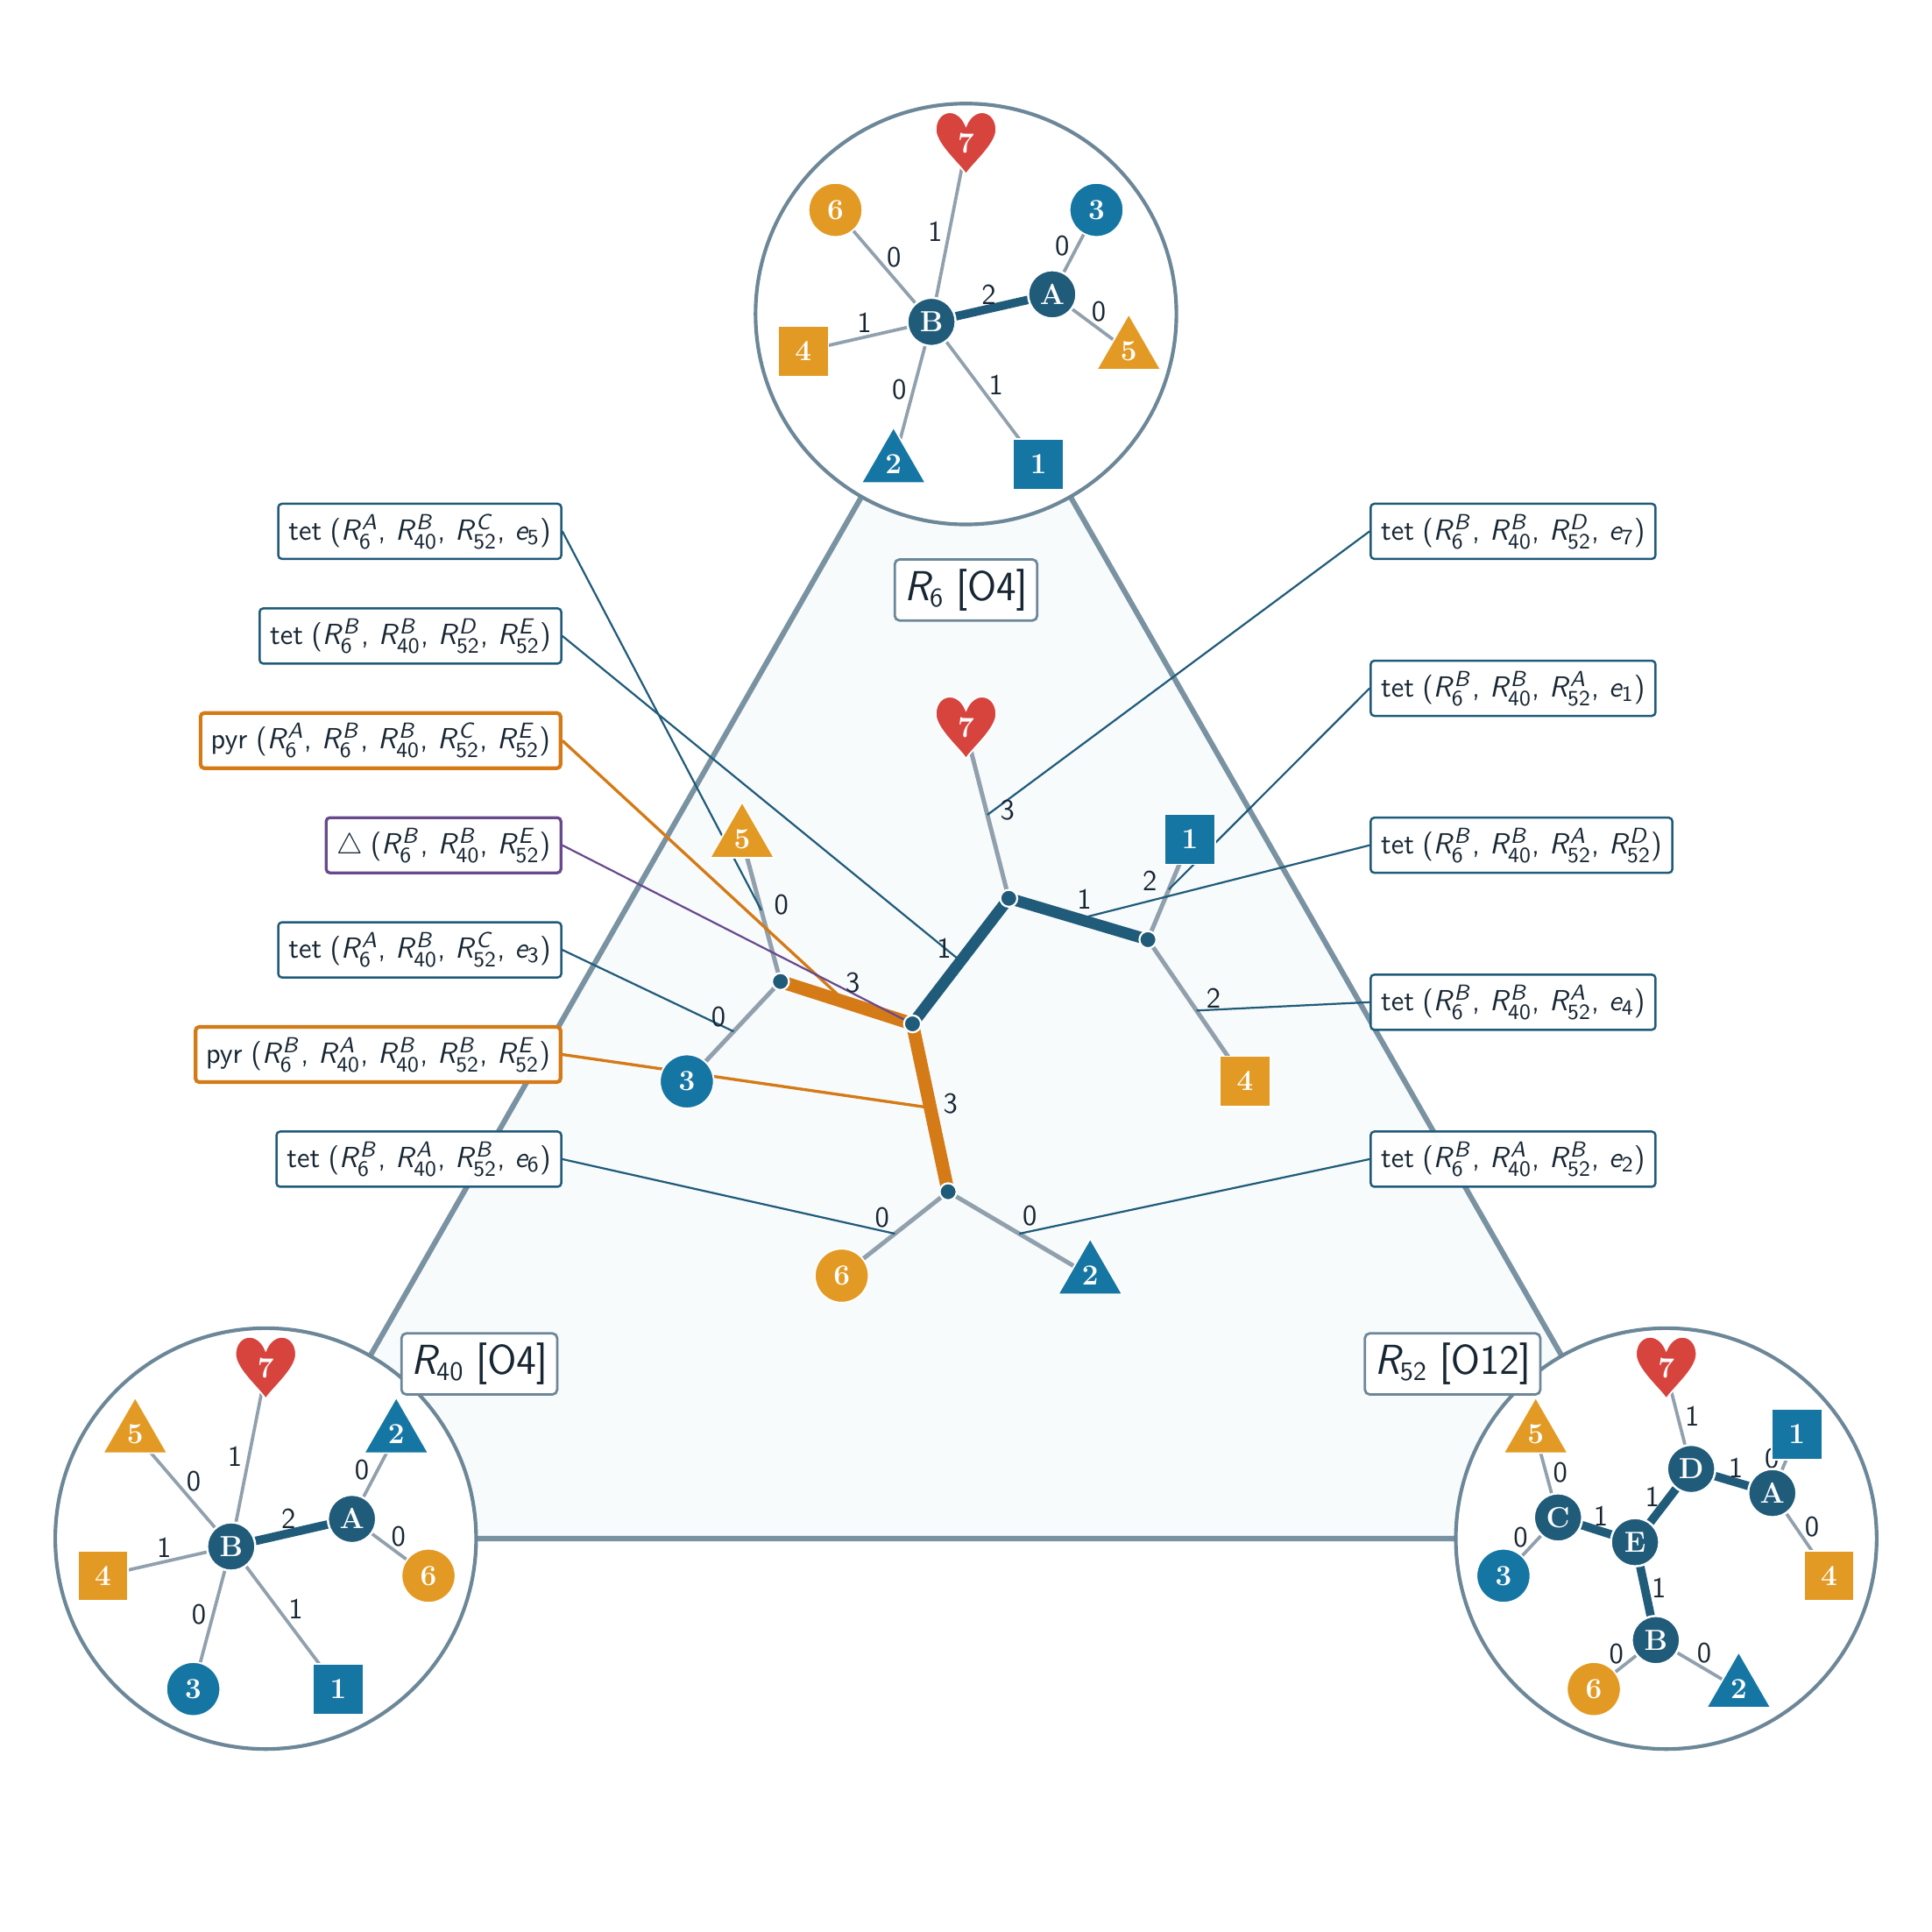
\begin{tikzpicture}[x=1cm,y=1cm]
\path[use as bounding box] (-13.65,-13.65) rectangle (13.65,13.65);
\path[support cell] (0.00000,9.45000)--(-10.15000,-8.30000)--(10.15000,-8.30000)--cycle;
\path[vertex disc] (0.00000,9.45000) circle[radius=3.05000cm];
\path[vertex disc] (-10.15000,-8.30000) circle[radius=3.05000cm];
\path[vertex disc] (10.15000,-8.30000) circle[radius=3.05000cm];
\coordinate (corner-1-v1) at (1.05000,7.26966);
\coordinate (corner-1-v2) at (-1.05000,7.26966);
\coordinate (corner-1-v3) at (1.89203,10.95885);
\coordinate (corner-1-v4) at (-2.35933,8.91150);
\coordinate (corner-1-v5) at (2.35933,8.91150);
\coordinate (corner-1-v6) at (-1.89203,10.95885);
\coordinate (corner-1-v7) at (0.00000,11.87000);
\coordinate (corner-1-v8) at (1.25040,9.73540);
\coordinate (corner-1-v9) at (-0.50016,9.33584);
\draw[internal edge] (corner-1-v8)--node[mini length,pos=0.5] {\(2\)}(corner-1-v9);
\draw[pendant edge] (corner-1-v1)--node[mini length,pos=0.5] {\(1\)}(corner-1-v9);
\draw[pendant edge] (corner-1-v2)--node[mini length,pos=0.5] {\(0\)}(corner-1-v9);
\draw[pendant edge] (corner-1-v3)--node[mini length,pos=0.5] {\(0\)}(corner-1-v8);
\draw[pendant edge] (corner-1-v4)--node[mini length,pos=0.5] {\(1\)}(corner-1-v9);
\draw[pendant edge] (corner-1-v5)--node[mini length,pos=0.5] {\(0\)}(corner-1-v8);
\draw[pendant edge] (corner-1-v6)--node[mini length,pos=0.5] {\(0\)}(corner-1-v9);
\draw[pendant edge] (corner-1-v7)--node[mini length,pos=0.5] {\(1\)}(corner-1-v9);
\node[lettered vertex] at (corner-1-v8) {A};
\node[lettered vertex] at (corner-1-v9) {B};
\taxonone{corner-1-v1}
\taxontwo{corner-1-v2}
\taxonthree{corner-1-v3}
\taxonfour{corner-1-v4}
\taxonfive{corner-1-v5}
\taxonsix{corner-1-v6}
\taxonseven{corner-1-v7}
\node[ray title] at (0.00000,5.45000) {\(R_{6}\;[\mathrm{O}4]\)};
\coordinate (corner-2-v1) at (-9.10000,-10.48034);
\coordinate (corner-2-v2) at (-8.25797,-6.79115);
\coordinate (corner-2-v3) at (-11.20000,-10.48034);
\coordinate (corner-2-v4) at (-12.50933,-8.83850);
\coordinate (corner-2-v5) at (-12.04203,-6.79115);
\coordinate (corner-2-v6) at (-7.79067,-8.83850);
\coordinate (corner-2-v7) at (-10.15000,-5.88000);
\coordinate (corner-2-v8) at (-8.89960,-8.01460);
\coordinate (corner-2-v9) at (-10.65016,-8.41416);
\draw[internal edge] (corner-2-v8)--node[mini length,pos=0.5] {\(2\)}(corner-2-v9);
\draw[pendant edge] (corner-2-v1)--node[mini length,pos=0.5] {\(1\)}(corner-2-v9);
\draw[pendant edge] (corner-2-v2)--node[mini length,pos=0.5] {\(0\)}(corner-2-v8);
\draw[pendant edge] (corner-2-v3)--node[mini length,pos=0.5] {\(0\)}(corner-2-v9);
\draw[pendant edge] (corner-2-v4)--node[mini length,pos=0.5] {\(1\)}(corner-2-v9);
\draw[pendant edge] (corner-2-v5)--node[mini length,pos=0.5] {\(0\)}(corner-2-v9);
\draw[pendant edge] (corner-2-v6)--node[mini length,pos=0.5] {\(0\)}(corner-2-v8);
\draw[pendant edge] (corner-2-v7)--node[mini length,pos=0.5] {\(1\)}(corner-2-v9);
\node[lettered vertex] at (corner-2-v8) {A};
\node[lettered vertex] at (corner-2-v9) {B};
\taxonone{corner-2-v1}
\taxontwo{corner-2-v2}
\taxonthree{corner-2-v3}
\taxonfour{corner-2-v4}
\taxonfive{corner-2-v5}
\taxonsix{corner-2-v6}
\taxonseven{corner-2-v7}
\node[ray title] at (-7.05349,-5.76788) {\(R_{40}\;[\mathrm{O}4]\)};
\coordinate (corner-3-v1) at (12.04203,-6.79115);
\coordinate (corner-3-v2) at (11.20000,-10.48034);
\coordinate (corner-3-v3) at (7.79067,-8.83850);
\coordinate (corner-3-v4) at (12.50933,-8.83850);
\coordinate (corner-3-v5) at (8.25797,-6.79115);
\coordinate (corner-3-v6) at (9.10000,-10.48034);
\coordinate (corner-3-v7) at (10.15000,-5.88000);
\coordinate (corner-3-v8) at (11.68773,-7.64009);
\coordinate (corner-3-v9) at (9.99924,-9.77081);
\coordinate (corner-3-v10) at (8.58212,-7.99380);
\coordinate (corner-3-v11) at (10.51182,-7.29061);
\coordinate (corner-3-v12) at (9.69773,-8.35174);
\draw[internal edge] (corner-3-v8)--node[mini length,pos=0.5] {\(1\)}(corner-3-v11);
\draw[internal edge] (corner-3-v9)--node[mini length,pos=0.5] {\(1\)}(corner-3-v12);
\draw[internal edge] (corner-3-v10)--node[mini length,pos=0.5] {\(1\)}(corner-3-v12);
\draw[internal edge] (corner-3-v11)--node[mini length,pos=0.5] {\(1\)}(corner-3-v12);
\draw[pendant edge] (corner-3-v1)--node[mini length,pos=0.5] {\(0\)}(corner-3-v8);
\draw[pendant edge] (corner-3-v2)--node[mini length,pos=0.5] {\(0\)}(corner-3-v9);
\draw[pendant edge] (corner-3-v3)--node[mini length,pos=0.5] {\(0\)}(corner-3-v10);
\draw[pendant edge] (corner-3-v4)--node[mini length,pos=0.5] {\(0\)}(corner-3-v8);
\draw[pendant edge] (corner-3-v5)--node[mini length,pos=0.5] {\(0\)}(corner-3-v10);
\draw[pendant edge] (corner-3-v6)--node[mini length,pos=0.5] {\(0\)}(corner-3-v9);
\draw[pendant edge] (corner-3-v7)--node[mini length,pos=0.5] {\(1\)}(corner-3-v11);
\node[lettered vertex] at (corner-3-v8) {A};
\node[lettered vertex] at (corner-3-v9) {B};
\node[lettered vertex] at (corner-3-v10) {C};
\node[lettered vertex] at (corner-3-v11) {D};
\node[lettered vertex] at (corner-3-v12) {E};
\taxonone{corner-3-v1}
\taxontwo{corner-3-v2}
\taxonthree{corner-3-v3}
\taxonfour{corner-3-v4}
\taxonfive{corner-3-v5}
\taxonsix{corner-3-v6}
\taxonseven{corner-3-v7}
\node[ray title] at (7.05349,-5.76788) {\(R_{52}\;[\mathrm{O}12]\)};
\coordinate (central-v1) at (3.24460,1.83748);
\coordinate (central-v2) at (1.80062,-4.48902);
\coordinate (central-v3) at (-4.04595,-1.67346);
\coordinate (central-v4) at (4.04595,-1.67346);
\coordinate (central-v5) at (-3.24460,1.83748);
\coordinate (central-v6) at (-1.80062,-4.48902);
\coordinate (central-v7) at (0.00000,3.40000);
\coordinate (central-v8) at (-0.25853,-3.27226);
\coordinate (central-v9) at (-2.68871,-0.22490);
\coordinate (central-v10) at (2.63701,0.38167);
\coordinate (central-v11) at (0.62047,0.98098);
\coordinate (central-v12) at (-0.77559,-0.83873);
\draw[central pyramid edge] (central-v8)--(central-v12);
\draw[central pyramid edge] (central-v9)--(central-v12);
\draw[central internal edge] (central-v10)--(central-v11);
\draw[central internal edge] (central-v11)--(central-v12);
\draw[central pendant edge] (central-v1)--(central-v10);
\draw[central pendant edge] (central-v2)--(central-v8);
\draw[central pendant edge] (central-v3)--(central-v9);
\draw[central pendant edge] (central-v4)--(central-v10);
\draw[central pendant edge] (central-v5)--(central-v9);
\draw[central pendant edge] (central-v6)--(central-v8);
\draw[central pendant edge] (central-v7)--(central-v11);
\draw[edge leader] (-5.85000,6.30000)--(-2.96666,0.80629);
\draw[edge leader] (-5.85000,4.78333)--(-0.07756,0.07113);
\draw[pyramid leader] (-5.85000,3.26667)--(-1.73215,-0.53181);
\draw[node leader] (-5.85000,1.75000)--(-0.77559,-0.83873);
\draw[edge leader] (-5.85000,0.23333)--(-3.36733,-0.94918);
\draw[pyramid leader] (-5.85000,-1.28333)--(-0.51706,-2.05549);
\draw[edge leader] (-5.85000,-2.80000)--(-1.02957,-3.88064);
\draw[edge leader] (5.85000,6.30000)--(0.31024,2.19049);
\draw[edge leader] (5.85000,4.02500)--(2.94080,1.10957);
\draw[edge leader] (5.85000,1.75000)--(1.62874,0.68132);
\draw[edge leader] (5.85000,-0.52500)--(3.34148,-0.64590);
\draw[edge leader] (5.85000,-2.80000)--(0.77104,-3.88064);
\node[internal vertex] at (central-v8) {};
\node[internal vertex] at (central-v9) {};
\node[internal vertex] at (central-v10) {};
\node[internal vertex] at (central-v11) {};
\node[internal vertex] at (central-v12) {};
\taxonone{central-v1}
\taxontwo{central-v2}
\taxonthree{central-v3}
\taxonfour{central-v4}
\taxonfive{central-v5}
\taxonsix{central-v6}
\taxonseven{central-v7}
\path (central-v8)--node[central length,pos=.50] {\(3\)}(central-v12);
\path (central-v9)--node[central length,pos=.50] {\(3\)}(central-v12);
\path (central-v10)--node[central length,pos=.50] {\(1\)}(central-v11);
\path (central-v11)--node[central length,pos=.50] {\(1\)}(central-v12);
\path (central-v1)--node[central length,pos=.50] {\(2\)}(central-v10);
\path (central-v2)--node[central length,pos=.50] {\(0\)}(central-v8);
\path (central-v3)--node[central length,pos=.50] {\(0\)}(central-v9);
\path (central-v4)--node[central length,pos=.50] {\(2\)}(central-v10);
\path (central-v5)--node[central length,pos=.50] {\(0\)}(central-v9);
\path (central-v6)--node[central length,pos=.50] {\(0\)}(central-v8);
\path (central-v7)--node[central length,pos=.50] {\(3\)}(central-v11);
\node[edge callout,anchor=east] (callout-1) at (-5.85000,6.30000) {\(\mathrm{tet}\;(R_{6}^{A},\,R_{40}^{B},\,R_{52}^{C},\,e_{5})\)};
\node[edge callout,anchor=east] (callout-2) at (-5.85000,4.78333) {\(\mathrm{tet}\;(R_{6}^{B},\,R_{40}^{B},\,R_{52}^{D},\,R_{52}^{E})\)};
\node[pyramid callout,anchor=east] (callout-3) at (-5.85000,3.26667) {\(\mathrm{pyr}\;(R_{6}^{A},\,R_{6}^{B},\,R_{40}^{B},\,R_{52}^{C},\,R_{52}^{E})\)};
\node[node callout,anchor=east] (callout-4) at (-5.85000,1.75000) {\(\triangle\;(R_{6}^{B},\,R_{40}^{B},\,R_{52}^{E})\)};
\node[edge callout,anchor=east] (callout-5) at (-5.85000,0.23333) {\(\mathrm{tet}\;(R_{6}^{A},\,R_{40}^{B},\,R_{52}^{C},\,e_{3})\)};
\node[pyramid callout,anchor=east] (callout-6) at (-5.85000,-1.28333) {\(\mathrm{pyr}\;(R_{6}^{B},\,R_{40}^{A},\,R_{40}^{B},\,R_{52}^{B},\,R_{52}^{E})\)};
\node[edge callout,anchor=east] (callout-7) at (-5.85000,-2.80000) {\(\mathrm{tet}\;(R_{6}^{B},\,R_{40}^{A},\,R_{52}^{B},\,e_{6})\)};
\node[edge callout,anchor=west] (callout-8) at (5.85000,6.30000) {\(\mathrm{tet}\;(R_{6}^{B},\,R_{40}^{B},\,R_{52}^{D},\,e_{7})\)};
\node[edge callout,anchor=west] (callout-9) at (5.85000,4.02500) {\(\mathrm{tet}\;(R_{6}^{B},\,R_{40}^{B},\,R_{52}^{A},\,e_{1})\)};
\node[edge callout,anchor=west] (callout-10) at (5.85000,1.75000) {\(\mathrm{tet}\;(R_{6}^{B},\,R_{40}^{B},\,R_{52}^{A},\,R_{52}^{D})\)};
\node[edge callout,anchor=west] (callout-11) at (5.85000,-0.52500) {\(\mathrm{tet}\;(R_{6}^{B},\,R_{40}^{B},\,R_{52}^{A},\,e_{4})\)};
\node[edge callout,anchor=west] (callout-12) at (5.85000,-2.80000) {\(\mathrm{tet}\;(R_{6}^{B},\,R_{40}^{A},\,R_{52}^{B},\,e_{2})\)};
\end{tikzpicture}\end{center}\vspace{-1mm}
\begin{atlasbox}\begin{atlaspanel}
\textcolor{toricgreen}{\bfseries PRIME TORIC}\quad \(P_{19}\):\enspace \(\square\ast\Delta_{2}\)\quad \(f=(7,19,26,19,7)\)\quad 14 lattice points
\end{atlaspanel}\end{atlasbox}
\clearpage
\begin{atlaspanel}[top=1mm,bottom=2mm]
\AtlasSupportOrbitSplit{%
\vspace*{-3mm}\mbox{{\LARGE\bfseries Triangle orbit 20}\hspace{3mm}\raisebox{.8mm}[0pt][0pt]{{\fontsize{16}{18}\selectfont\color{muted}size 3}}}%
}{%
\vspace*{-3mm}{\fontsize{13}{16}\selectfont{\color{animalblue}\bfseries\(\mathbb{F}_2\) only}\quad{\color{muted}\(\underline{\{9,\,34,\,52\}}\), \(\{8,\,30,\,53\}\), \(\{10,\,33,\,54\}\)}\rule[-3mm]{0pt}{3mm}}%
}%
\end{atlaspanel}\vspace{2mm}
\begin{center}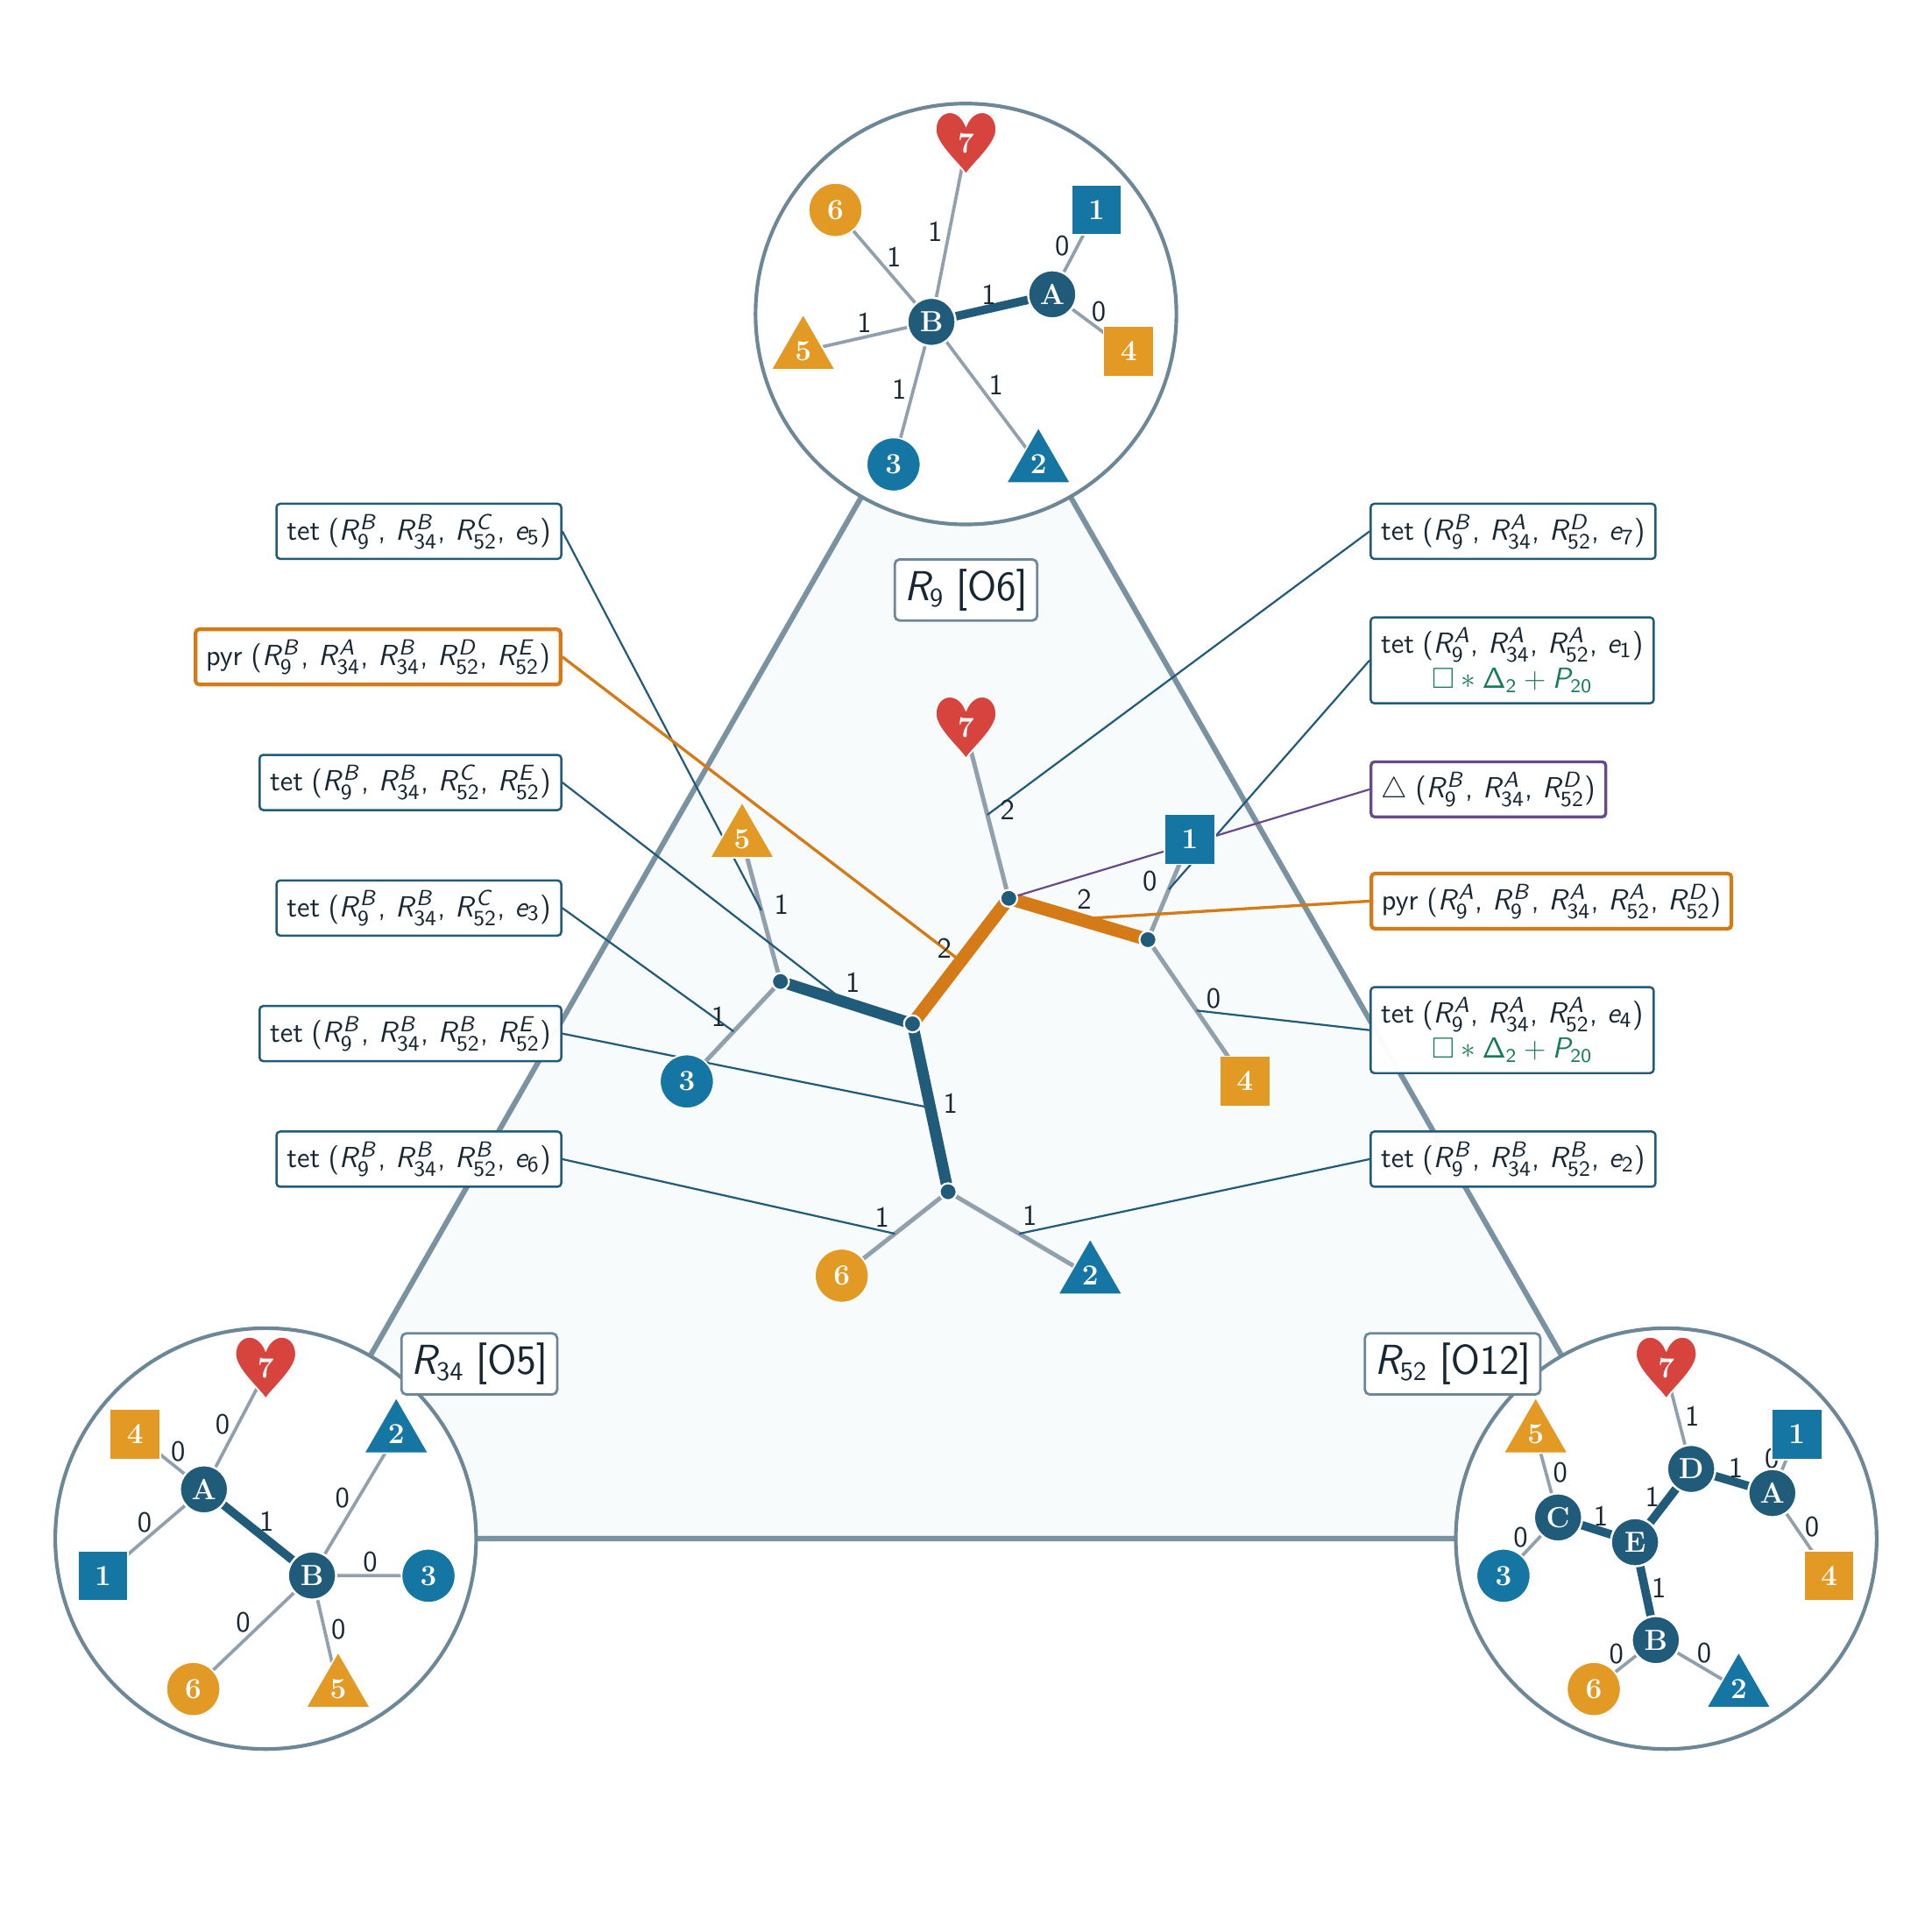
\begin{tikzpicture}[x=1cm,y=1cm]
\path[use as bounding box] (-13.65,-13.65) rectangle (13.65,13.65);
\path[support cell] (0.00000,9.45000)--(-10.15000,-8.30000)--(10.15000,-8.30000)--cycle;
\path[vertex disc] (0.00000,9.45000) circle[radius=3.05000cm];
\path[vertex disc] (-10.15000,-8.30000) circle[radius=3.05000cm];
\path[vertex disc] (10.15000,-8.30000) circle[radius=3.05000cm];
\coordinate (corner-1-v1) at (1.89203,10.95885);
\coordinate (corner-1-v2) at (1.05000,7.26966);
\coordinate (corner-1-v3) at (-1.05000,7.26966);
\coordinate (corner-1-v4) at (2.35933,8.91150);
\coordinate (corner-1-v5) at (-2.35933,8.91150);
\coordinate (corner-1-v6) at (-1.89203,10.95885);
\coordinate (corner-1-v7) at (0.00000,11.87000);
\coordinate (corner-1-v8) at (1.25040,9.73540);
\coordinate (corner-1-v9) at (-0.50016,9.33584);
\draw[internal edge] (corner-1-v8)--node[mini length,pos=0.5] {\(1\)}(corner-1-v9);
\draw[pendant edge] (corner-1-v1)--node[mini length,pos=0.5] {\(0\)}(corner-1-v8);
\draw[pendant edge] (corner-1-v2)--node[mini length,pos=0.5] {\(1\)}(corner-1-v9);
\draw[pendant edge] (corner-1-v3)--node[mini length,pos=0.5] {\(1\)}(corner-1-v9);
\draw[pendant edge] (corner-1-v4)--node[mini length,pos=0.5] {\(0\)}(corner-1-v8);
\draw[pendant edge] (corner-1-v5)--node[mini length,pos=0.5] {\(1\)}(corner-1-v9);
\draw[pendant edge] (corner-1-v6)--node[mini length,pos=0.5] {\(1\)}(corner-1-v9);
\draw[pendant edge] (corner-1-v7)--node[mini length,pos=0.5] {\(1\)}(corner-1-v9);
\node[lettered vertex] at (corner-1-v8) {A};
\node[lettered vertex] at (corner-1-v9) {B};
\taxonone{corner-1-v1}
\taxontwo{corner-1-v2}
\taxonthree{corner-1-v3}
\taxonfour{corner-1-v4}
\taxonfive{corner-1-v5}
\taxonsix{corner-1-v6}
\taxonseven{corner-1-v7}
\node[ray title] at (0.00000,5.45000) {\(R_{9}\;[\mathrm{O}6]\)};
\coordinate (corner-2-v1) at (-12.50933,-8.83850);
\coordinate (corner-2-v2) at (-8.25797,-6.79115);
\coordinate (corner-2-v3) at (-7.79067,-8.83850);
\coordinate (corner-2-v4) at (-12.04203,-6.79115);
\coordinate (corner-2-v5) at (-9.10000,-10.48034);
\coordinate (corner-2-v6) at (-11.20000,-10.48034);
\coordinate (corner-2-v7) at (-10.15000,-5.88000);
\coordinate (corner-2-v8) at (-11.04502,-7.58624);
\coordinate (corner-2-v9) at (-9.47873,-8.83532);
\draw[internal edge] (corner-2-v8)--node[mini length,pos=0.5] {\(1\)}(corner-2-v9);
\draw[pendant edge] (corner-2-v1)--node[mini length,pos=0.5] {\(0\)}(corner-2-v8);
\draw[pendant edge] (corner-2-v2)--node[mini length,pos=0.5] {\(0\)}(corner-2-v9);
\draw[pendant edge] (corner-2-v3)--node[mini length,pos=0.5] {\(0\)}(corner-2-v9);
\draw[pendant edge] (corner-2-v4)--node[mini length,pos=0.5] {\(0\)}(corner-2-v8);
\draw[pendant edge] (corner-2-v5)--node[mini length,pos=0.5] {\(0\)}(corner-2-v9);
\draw[pendant edge] (corner-2-v6)--node[mini length,pos=0.5] {\(0\)}(corner-2-v9);
\draw[pendant edge] (corner-2-v7)--node[mini length,pos=0.5] {\(0\)}(corner-2-v8);
\node[lettered vertex] at (corner-2-v8) {A};
\node[lettered vertex] at (corner-2-v9) {B};
\taxonone{corner-2-v1}
\taxontwo{corner-2-v2}
\taxonthree{corner-2-v3}
\taxonfour{corner-2-v4}
\taxonfive{corner-2-v5}
\taxonsix{corner-2-v6}
\taxonseven{corner-2-v7}
\node[ray title] at (-7.05349,-5.76788) {\(R_{34}\;[\mathrm{O}5]\)};
\coordinate (corner-3-v1) at (12.04203,-6.79115);
\coordinate (corner-3-v2) at (11.20000,-10.48034);
\coordinate (corner-3-v3) at (7.79067,-8.83850);
\coordinate (corner-3-v4) at (12.50933,-8.83850);
\coordinate (corner-3-v5) at (8.25797,-6.79115);
\coordinate (corner-3-v6) at (9.10000,-10.48034);
\coordinate (corner-3-v7) at (10.15000,-5.88000);
\coordinate (corner-3-v8) at (11.68773,-7.64009);
\coordinate (corner-3-v9) at (9.99924,-9.77081);
\coordinate (corner-3-v10) at (8.58212,-7.99380);
\coordinate (corner-3-v11) at (10.51182,-7.29061);
\coordinate (corner-3-v12) at (9.69773,-8.35174);
\draw[internal edge] (corner-3-v8)--node[mini length,pos=0.5] {\(1\)}(corner-3-v11);
\draw[internal edge] (corner-3-v9)--node[mini length,pos=0.5] {\(1\)}(corner-3-v12);
\draw[internal edge] (corner-3-v10)--node[mini length,pos=0.5] {\(1\)}(corner-3-v12);
\draw[internal edge] (corner-3-v11)--node[mini length,pos=0.5] {\(1\)}(corner-3-v12);
\draw[pendant edge] (corner-3-v1)--node[mini length,pos=0.5] {\(0\)}(corner-3-v8);
\draw[pendant edge] (corner-3-v2)--node[mini length,pos=0.5] {\(0\)}(corner-3-v9);
\draw[pendant edge] (corner-3-v3)--node[mini length,pos=0.5] {\(0\)}(corner-3-v10);
\draw[pendant edge] (corner-3-v4)--node[mini length,pos=0.5] {\(0\)}(corner-3-v8);
\draw[pendant edge] (corner-3-v5)--node[mini length,pos=0.5] {\(0\)}(corner-3-v10);
\draw[pendant edge] (corner-3-v6)--node[mini length,pos=0.5] {\(0\)}(corner-3-v9);
\draw[pendant edge] (corner-3-v7)--node[mini length,pos=0.5] {\(1\)}(corner-3-v11);
\node[lettered vertex] at (corner-3-v8) {A};
\node[lettered vertex] at (corner-3-v9) {B};
\node[lettered vertex] at (corner-3-v10) {C};
\node[lettered vertex] at (corner-3-v11) {D};
\node[lettered vertex] at (corner-3-v12) {E};
\taxonone{corner-3-v1}
\taxontwo{corner-3-v2}
\taxonthree{corner-3-v3}
\taxonfour{corner-3-v4}
\taxonfive{corner-3-v5}
\taxonsix{corner-3-v6}
\taxonseven{corner-3-v7}
\node[ray title] at (7.05349,-5.76788) {\(R_{52}\;[\mathrm{O}12]\)};
\coordinate (central-v1) at (3.24460,1.83748);
\coordinate (central-v2) at (1.80062,-4.48902);
\coordinate (central-v3) at (-4.04595,-1.67346);
\coordinate (central-v4) at (4.04595,-1.67346);
\coordinate (central-v5) at (-3.24460,1.83748);
\coordinate (central-v6) at (-1.80062,-4.48902);
\coordinate (central-v7) at (0.00000,3.40000);
\coordinate (central-v8) at (2.63701,0.38167);
\coordinate (central-v9) at (0.62047,0.98098);
\coordinate (central-v10) at (-0.25853,-3.27226);
\coordinate (central-v11) at (-2.68871,-0.22490);
\coordinate (central-v12) at (-0.77559,-0.83873);
\draw[central pyramid edge] (central-v8)--(central-v9);
\draw[central pyramid edge] (central-v9)--(central-v12);
\draw[central internal edge] (central-v10)--(central-v12);
\draw[central internal edge] (central-v11)--(central-v12);
\draw[central pendant edge] (central-v1)--(central-v8);
\draw[central pendant edge] (central-v2)--(central-v10);
\draw[central pendant edge] (central-v3)--(central-v11);
\draw[central pendant edge] (central-v4)--(central-v8);
\draw[central pendant edge] (central-v5)--(central-v11);
\draw[central pendant edge] (central-v6)--(central-v10);
\draw[central pendant edge] (central-v7)--(central-v9);
\draw[edge leader] (-5.85000,6.30000)--(-2.96666,0.80629);
\draw[pyramid leader] (-5.85000,4.48000)--(-0.07756,0.07113);
\draw[edge leader] (-5.85000,2.66000)--(-1.73215,-0.53181);
\draw[edge leader] (-5.85000,0.84000)--(-3.36733,-0.94918);
\draw[edge leader] (-5.85000,-0.98000)--(-0.51706,-2.05549);
\draw[edge leader] (-5.85000,-2.80000)--(-1.02957,-3.88064);
\draw[edge leader] (5.85000,6.30000)--(0.31024,2.19049);
\draw[edge leader] (5.85000,4.43000)--(2.94080,1.10957);
\draw[node leader] (5.85000,2.56000)--(0.62047,0.98098);
\draw[pyramid leader] (5.85000,0.94000)--(1.62874,0.68132);
\draw[edge leader] (5.85000,-0.93000)--(3.34148,-0.64590);
\draw[edge leader] (5.85000,-2.80000)--(0.77104,-3.88064);
\node[internal vertex] at (central-v8) {};
\node[internal vertex] at (central-v9) {};
\node[internal vertex] at (central-v10) {};
\node[internal vertex] at (central-v11) {};
\node[internal vertex] at (central-v12) {};
\taxonone{central-v1}
\taxontwo{central-v2}
\taxonthree{central-v3}
\taxonfour{central-v4}
\taxonfive{central-v5}
\taxonsix{central-v6}
\taxonseven{central-v7}
\path (central-v8)--node[central length,pos=.50] {\(2\)}(central-v9);
\path (central-v9)--node[central length,pos=.50] {\(2\)}(central-v12);
\path (central-v10)--node[central length,pos=.50] {\(1\)}(central-v12);
\path (central-v11)--node[central length,pos=.50] {\(1\)}(central-v12);
\path (central-v1)--node[central length,pos=.50] {\(0\)}(central-v8);
\path (central-v2)--node[central length,pos=.50] {\(1\)}(central-v10);
\path (central-v3)--node[central length,pos=.50] {\(1\)}(central-v11);
\path (central-v4)--node[central length,pos=.50] {\(0\)}(central-v8);
\path (central-v5)--node[central length,pos=.50] {\(1\)}(central-v11);
\path (central-v6)--node[central length,pos=.50] {\(1\)}(central-v10);
\path (central-v7)--node[central length,pos=.50] {\(2\)}(central-v9);
\node[edge callout,anchor=east] (callout-1) at (-5.85000,6.30000) {\(\mathrm{tet}\;(R_{9}^{B},\,R_{34}^{B},\,R_{52}^{C},\,e_{5})\)};
\node[pyramid callout,anchor=east] (callout-2) at (-5.85000,4.48000) {\(\mathrm{pyr}\;(R_{9}^{B},\,R_{34}^{A},\,R_{34}^{B},\,R_{52}^{D},\,R_{52}^{E})\)};
\node[edge callout,anchor=east] (callout-3) at (-5.85000,2.66000) {\(\mathrm{tet}\;(R_{9}^{B},\,R_{34}^{B},\,R_{52}^{C},\,R_{52}^{E})\)};
\node[edge callout,anchor=east] (callout-4) at (-5.85000,0.84000) {\(\mathrm{tet}\;(R_{9}^{B},\,R_{34}^{B},\,R_{52}^{C},\,e_{3})\)};
\node[edge callout,anchor=east] (callout-5) at (-5.85000,-0.98000) {\(\mathrm{tet}\;(R_{9}^{B},\,R_{34}^{B},\,R_{52}^{B},\,R_{52}^{E})\)};
\node[edge callout,anchor=east] (callout-6) at (-5.85000,-2.80000) {\(\mathrm{tet}\;(R_{9}^{B},\,R_{34}^{B},\,R_{52}^{B},\,e_{6})\)};
\node[edge callout,anchor=west] (callout-7) at (5.85000,6.30000) {\(\mathrm{tet}\;(R_{9}^{B},\,R_{34}^{A},\,R_{52}^{D},\,e_{7})\)};
\node[edge callout,anchor=west] (callout-8) at (5.85000,4.43000) {\(\mathrm{tet}\;(R_{9}^{A},\,R_{34}^{A},\,R_{52}^{A},\,e_{1})\)\\{\fontsize{12}{14}\selectfont\color{toricgreen}\(\square\ast\Delta_{2}+P_{20}\)}};
\node[node callout,anchor=west] (callout-9) at (5.85000,2.56000) {\(\triangle\;(R_{9}^{B},\,R_{34}^{A},\,R_{52}^{D})\)};
\node[pyramid callout,anchor=west] (callout-10) at (5.85000,0.94000) {\(\mathrm{pyr}\;(R_{9}^{A},\,R_{9}^{B},\,R_{34}^{A},\,R_{52}^{A},\,R_{52}^{D})\)};
\node[edge callout,anchor=west] (callout-11) at (5.85000,-0.93000) {\(\mathrm{tet}\;(R_{9}^{A},\,R_{34}^{A},\,R_{52}^{A},\,e_{4})\)\\{\fontsize{12}{14}\selectfont\color{toricgreen}\(\square\ast\Delta_{2}+P_{20}\)}};
\node[edge callout,anchor=west] (callout-12) at (5.85000,-2.80000) {\(\mathrm{tet}\;(R_{9}^{B},\,R_{34}^{B},\,R_{52}^{B},\,e_{2})\)};
\end{tikzpicture}\end{center}\vspace{-1mm}
\begin{atlasbox}\begin{atlaspanel}
\textcolor{toricgreen}{\bfseries PRIME TORIC}\quad \(P_{20}\):\enspace \(\mathrm{Wed}(\square\ast\Delta_{0};\,\Delta_1)\ast\Delta_{0}\)\quad \(f=(9,26,35,24,8)\)\quad 15 lattice points
\end{atlaspanel}\end{atlasbox}
\clearpage
\begin{atlaspanel}[top=1mm,bottom=2mm]
\AtlasSupportOrbitSplit{%
\vspace*{-3mm}\mbox{{\LARGE\bfseries Triangle orbit 21}\hspace{3mm}\raisebox{.8mm}[0pt][0pt]{{\fontsize{16}{18}\selectfont\color{muted}size 2}}}%
}{%
\vspace*{-3mm}{\fontsize{13}{16}\selectfont{\color{muted}\(\mathbb{Q}\) and \(\mathbb{F}_2\)}\quad{\color{muted}\(\underline{\{7,\,12,\,40\}}\), \(\{6,\,11,\,41\}\)}\rule[-3mm]{0pt}{3mm}}%
}%
\end{atlaspanel}\vspace{2mm}
\begin{center}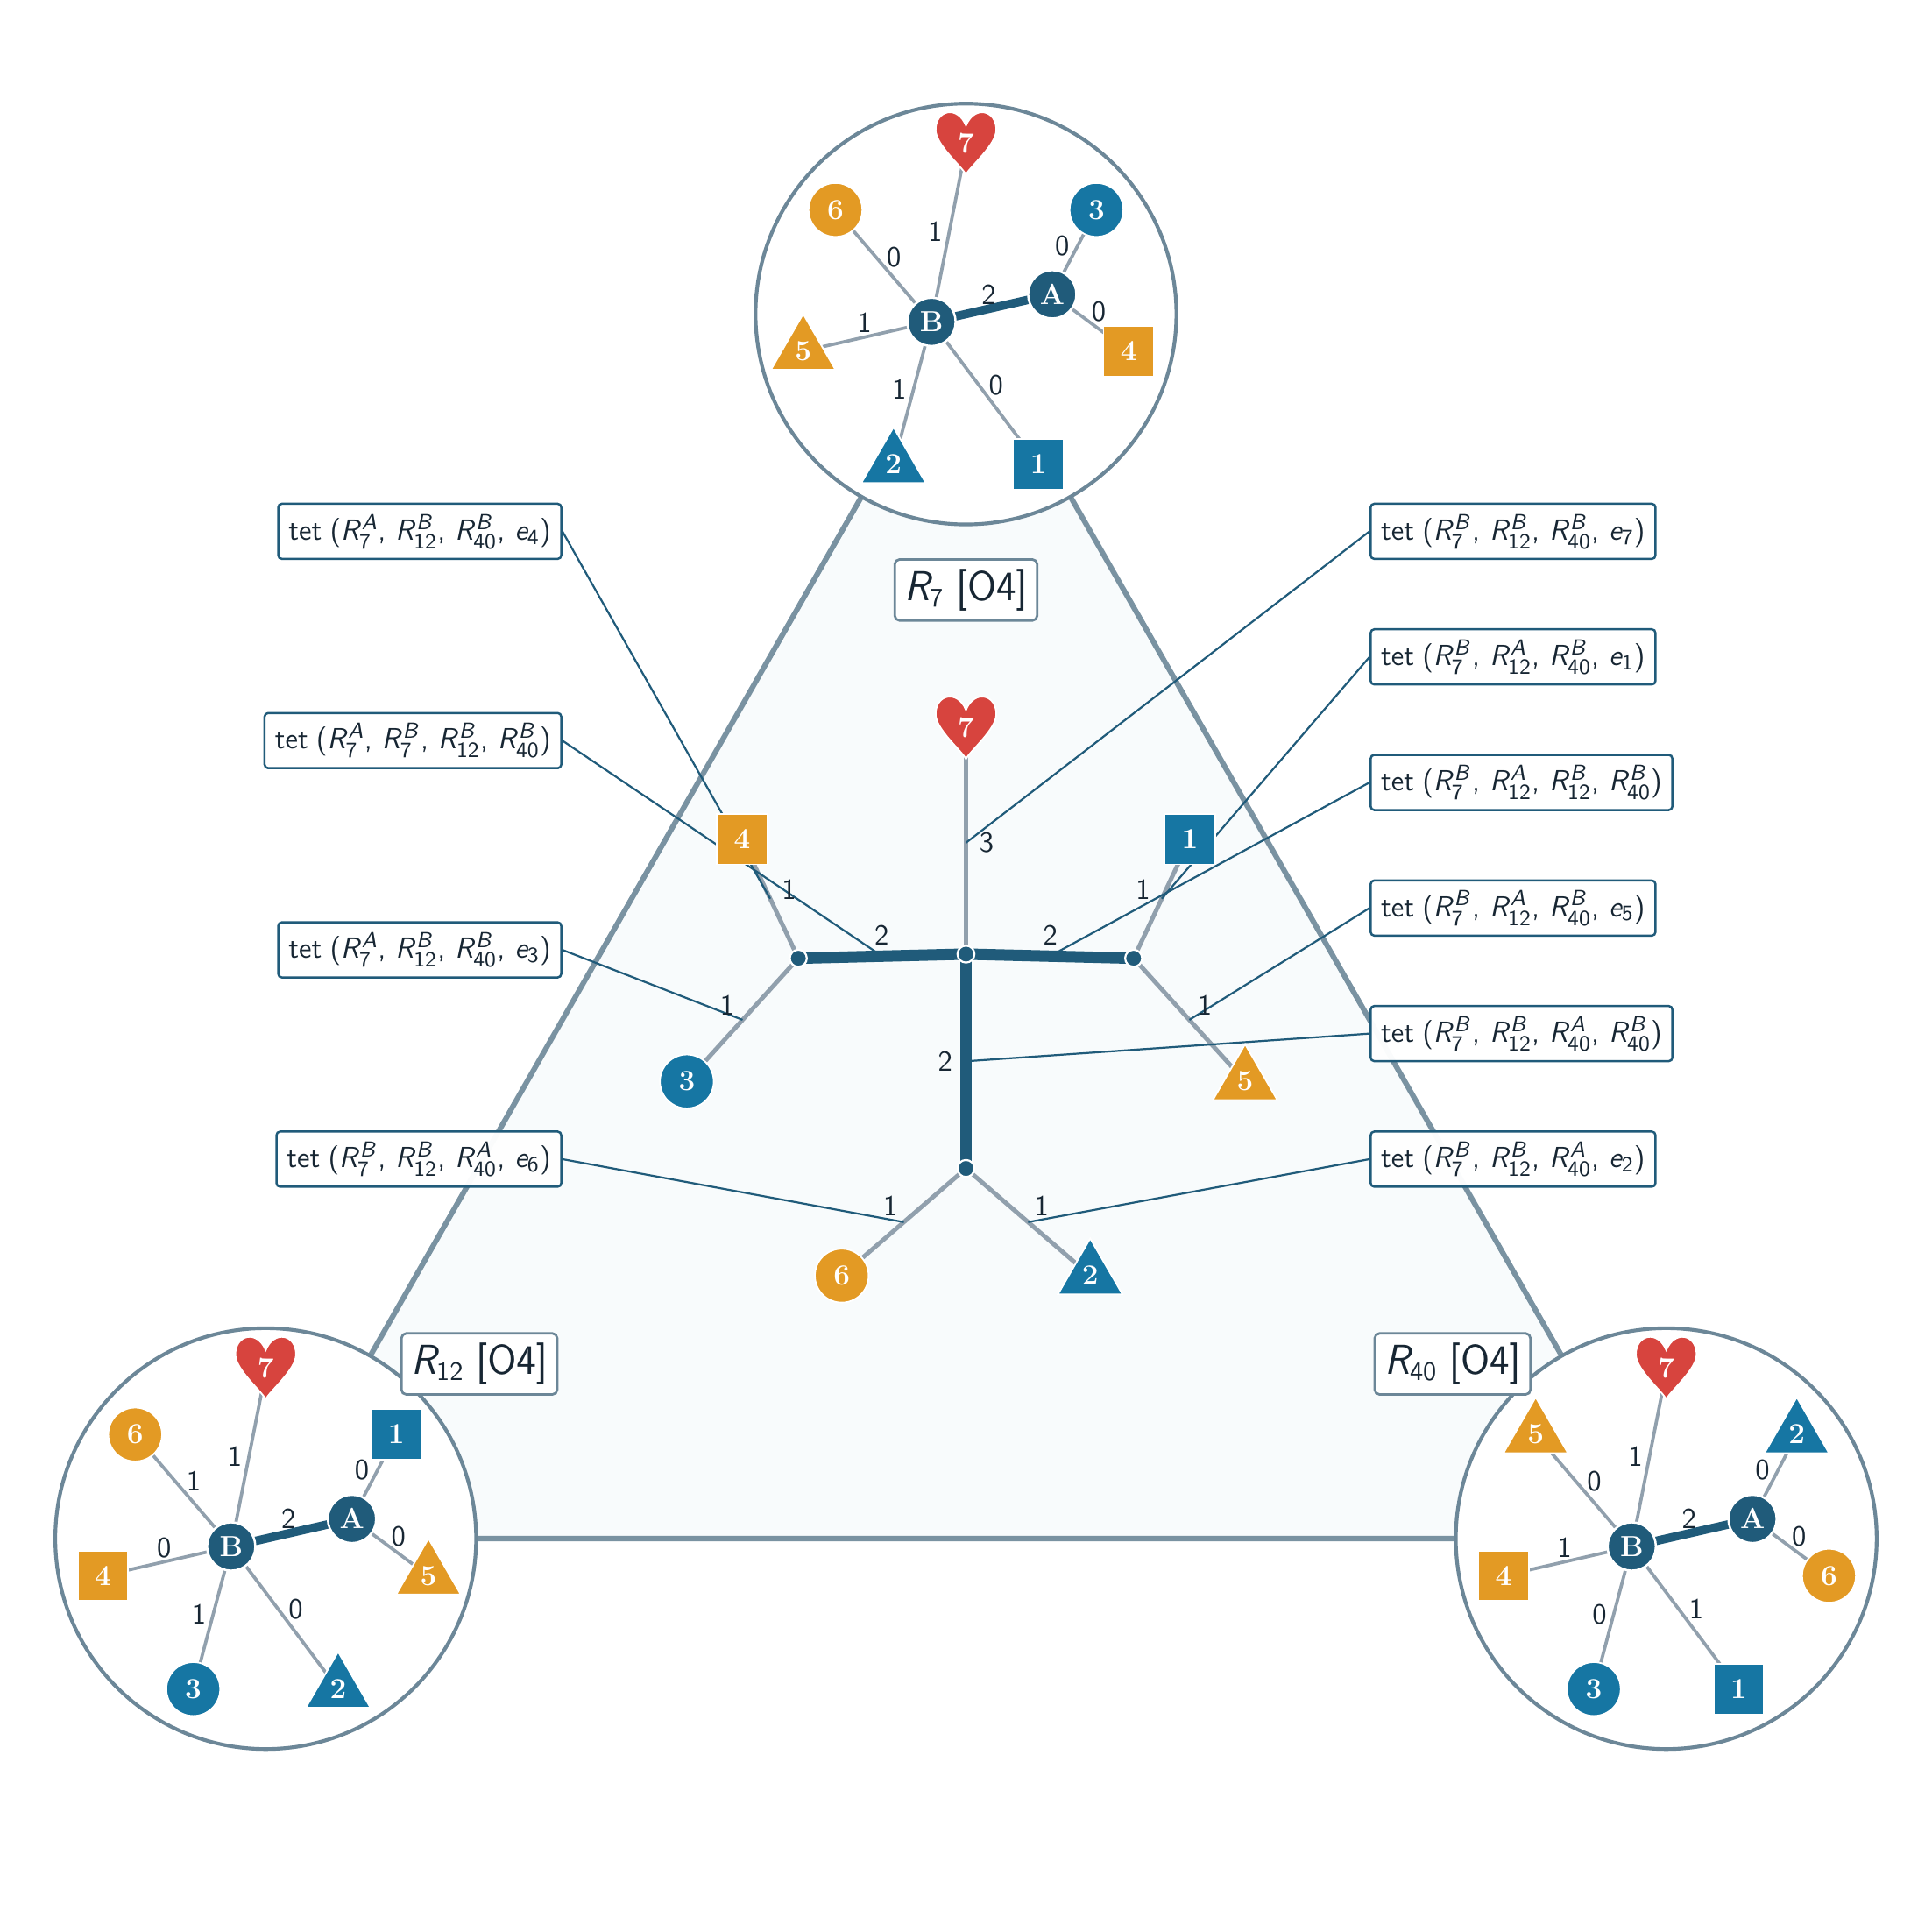
\begin{tikzpicture}[x=1cm,y=1cm]
\path[use as bounding box] (-13.65,-13.65) rectangle (13.65,13.65);
\path[support cell] (0.00000,9.45000)--(-10.15000,-8.30000)--(10.15000,-8.30000)--cycle;
\path[vertex disc] (0.00000,9.45000) circle[radius=3.05000cm];
\path[vertex disc] (-10.15000,-8.30000) circle[radius=3.05000cm];
\path[vertex disc] (10.15000,-8.30000) circle[radius=3.05000cm];
\coordinate (corner-1-v1) at (1.05000,7.26966);
\coordinate (corner-1-v2) at (-1.05000,7.26966);
\coordinate (corner-1-v3) at (1.89203,10.95885);
\coordinate (corner-1-v4) at (2.35933,8.91150);
\coordinate (corner-1-v5) at (-2.35933,8.91150);
\coordinate (corner-1-v6) at (-1.89203,10.95885);
\coordinate (corner-1-v7) at (0.00000,11.87000);
\coordinate (corner-1-v8) at (1.25040,9.73540);
\coordinate (corner-1-v9) at (-0.50016,9.33584);
\draw[internal edge] (corner-1-v8)--node[mini length,pos=0.5] {\(2\)}(corner-1-v9);
\draw[pendant edge] (corner-1-v1)--node[mini length,pos=0.5] {\(0\)}(corner-1-v9);
\draw[pendant edge] (corner-1-v2)--node[mini length,pos=0.5] {\(1\)}(corner-1-v9);
\draw[pendant edge] (corner-1-v3)--node[mini length,pos=0.5] {\(0\)}(corner-1-v8);
\draw[pendant edge] (corner-1-v4)--node[mini length,pos=0.5] {\(0\)}(corner-1-v8);
\draw[pendant edge] (corner-1-v5)--node[mini length,pos=0.5] {\(1\)}(corner-1-v9);
\draw[pendant edge] (corner-1-v6)--node[mini length,pos=0.5] {\(0\)}(corner-1-v9);
\draw[pendant edge] (corner-1-v7)--node[mini length,pos=0.5] {\(1\)}(corner-1-v9);
\node[lettered vertex] at (corner-1-v8) {A};
\node[lettered vertex] at (corner-1-v9) {B};
\taxonone{corner-1-v1}
\taxontwo{corner-1-v2}
\taxonthree{corner-1-v3}
\taxonfour{corner-1-v4}
\taxonfive{corner-1-v5}
\taxonsix{corner-1-v6}
\taxonseven{corner-1-v7}
\node[ray title] at (0.00000,5.45000) {\(R_{7}\;[\mathrm{O}4]\)};
\coordinate (corner-2-v1) at (-8.25797,-6.79115);
\coordinate (corner-2-v2) at (-9.10000,-10.48034);
\coordinate (corner-2-v3) at (-11.20000,-10.48034);
\coordinate (corner-2-v4) at (-12.50933,-8.83850);
\coordinate (corner-2-v5) at (-7.79067,-8.83850);
\coordinate (corner-2-v6) at (-12.04203,-6.79115);
\coordinate (corner-2-v7) at (-10.15000,-5.88000);
\coordinate (corner-2-v8) at (-8.89960,-8.01460);
\coordinate (corner-2-v9) at (-10.65016,-8.41416);
\draw[internal edge] (corner-2-v8)--node[mini length,pos=0.5] {\(2\)}(corner-2-v9);
\draw[pendant edge] (corner-2-v1)--node[mini length,pos=0.5] {\(0\)}(corner-2-v8);
\draw[pendant edge] (corner-2-v2)--node[mini length,pos=0.5] {\(0\)}(corner-2-v9);
\draw[pendant edge] (corner-2-v3)--node[mini length,pos=0.5] {\(1\)}(corner-2-v9);
\draw[pendant edge] (corner-2-v4)--node[mini length,pos=0.5] {\(0\)}(corner-2-v9);
\draw[pendant edge] (corner-2-v5)--node[mini length,pos=0.5] {\(0\)}(corner-2-v8);
\draw[pendant edge] (corner-2-v6)--node[mini length,pos=0.5] {\(1\)}(corner-2-v9);
\draw[pendant edge] (corner-2-v7)--node[mini length,pos=0.5] {\(1\)}(corner-2-v9);
\node[lettered vertex] at (corner-2-v8) {A};
\node[lettered vertex] at (corner-2-v9) {B};
\taxonone{corner-2-v1}
\taxontwo{corner-2-v2}
\taxonthree{corner-2-v3}
\taxonfour{corner-2-v4}
\taxonfive{corner-2-v5}
\taxonsix{corner-2-v6}
\taxonseven{corner-2-v7}
\node[ray title] at (-7.05349,-5.76788) {\(R_{12}\;[\mathrm{O}4]\)};
\coordinate (corner-3-v1) at (11.20000,-10.48034);
\coordinate (corner-3-v2) at (12.04203,-6.79115);
\coordinate (corner-3-v3) at (9.10000,-10.48034);
\coordinate (corner-3-v4) at (7.79067,-8.83850);
\coordinate (corner-3-v5) at (8.25797,-6.79115);
\coordinate (corner-3-v6) at (12.50933,-8.83850);
\coordinate (corner-3-v7) at (10.15000,-5.88000);
\coordinate (corner-3-v8) at (11.40040,-8.01460);
\coordinate (corner-3-v9) at (9.64984,-8.41416);
\draw[internal edge] (corner-3-v8)--node[mini length,pos=0.5] {\(2\)}(corner-3-v9);
\draw[pendant edge] (corner-3-v1)--node[mini length,pos=0.5] {\(1\)}(corner-3-v9);
\draw[pendant edge] (corner-3-v2)--node[mini length,pos=0.5] {\(0\)}(corner-3-v8);
\draw[pendant edge] (corner-3-v3)--node[mini length,pos=0.5] {\(0\)}(corner-3-v9);
\draw[pendant edge] (corner-3-v4)--node[mini length,pos=0.5] {\(1\)}(corner-3-v9);
\draw[pendant edge] (corner-3-v5)--node[mini length,pos=0.5] {\(0\)}(corner-3-v9);
\draw[pendant edge] (corner-3-v6)--node[mini length,pos=0.5] {\(0\)}(corner-3-v8);
\draw[pendant edge] (corner-3-v7)--node[mini length,pos=0.5] {\(1\)}(corner-3-v9);
\node[lettered vertex] at (corner-3-v8) {A};
\node[lettered vertex] at (corner-3-v9) {B};
\taxonone{corner-3-v1}
\taxontwo{corner-3-v2}
\taxonthree{corner-3-v3}
\taxonfour{corner-3-v4}
\taxonfive{corner-3-v5}
\taxonsix{corner-3-v6}
\taxonseven{corner-3-v7}
\node[ray title] at (7.05349,-5.76788) {\(R_{40}\;[\mathrm{O}4]\)};
\coordinate (central-v1) at (3.24460,1.83748);
\coordinate (central-v2) at (1.80062,-4.48902);
\coordinate (central-v3) at (-4.04595,-1.67346);
\coordinate (central-v4) at (-3.24460,1.83748);
\coordinate (central-v5) at (4.04595,-1.67346);
\coordinate (central-v6) at (-1.80062,-4.48902);
\coordinate (central-v7) at (0.00000,3.40000);
\coordinate (central-v8) at (2.43018,0.11208);
\coordinate (central-v9) at (0.00000,-2.93527);
\coordinate (central-v10) at (-2.43018,0.11208);
\coordinate (central-v11) at (0.00000,0.17222);
\draw[central internal edge] (central-v8)--(central-v11);
\draw[central internal edge] (central-v9)--(central-v11);
\draw[central internal edge] (central-v10)--(central-v11);
\draw[central pendant edge] (central-v1)--(central-v8);
\draw[central pendant edge] (central-v2)--(central-v9);
\draw[central pendant edge] (central-v3)--(central-v10);
\draw[central pendant edge] (central-v4)--(central-v10);
\draw[central pendant edge] (central-v5)--(central-v8);
\draw[central pendant edge] (central-v6)--(central-v9);
\draw[central pendant edge] (central-v7)--(central-v11);
\draw[edge leader] (-5.85000,6.30000)--(-2.83739,0.97478);
\draw[edge leader] (-5.85000,3.26667)--(-1.21509,0.14215);
\draw[edge leader] (-5.85000,0.23333)--(-3.23807,-0.78069);
\draw[edge leader] (-5.85000,-2.80000)--(-0.90031,-3.71215);
\draw[edge leader] (5.85000,6.30000)--(0.00000,1.78611);
\draw[edge leader] (5.85000,4.48000)--(2.83739,0.97478);
\draw[edge leader] (5.85000,2.66000)--(1.21509,0.14215);
\draw[edge leader] (5.85000,0.84000)--(3.23807,-0.78069);
\draw[edge leader] (5.85000,-0.98000)--(0.00000,-1.38153);
\draw[edge leader] (5.85000,-2.80000)--(0.90031,-3.71215);
\node[internal vertex] at (central-v8) {};
\node[internal vertex] at (central-v9) {};
\node[internal vertex] at (central-v10) {};
\node[internal vertex] at (central-v11) {};
\taxonone{central-v1}
\taxontwo{central-v2}
\taxonthree{central-v3}
\taxonfour{central-v4}
\taxonfive{central-v5}
\taxonsix{central-v6}
\taxonseven{central-v7}
\path (central-v8)--node[central length,pos=.50] {\(2\)}(central-v11);
\path (central-v9)--node[central length,pos=.50] {\(2\)}(central-v11);
\path (central-v10)--node[central length,pos=.50] {\(2\)}(central-v11);
\path (central-v1)--node[central length,pos=.50] {\(1\)}(central-v8);
\path (central-v2)--node[central length,pos=.50] {\(1\)}(central-v9);
\path (central-v3)--node[central length,pos=.50] {\(1\)}(central-v10);
\path (central-v4)--node[central length,pos=.50] {\(1\)}(central-v10);
\path (central-v5)--node[central length,pos=.50] {\(1\)}(central-v8);
\path (central-v6)--node[central length,pos=.50] {\(1\)}(central-v9);
\path (central-v7)--node[central length,pos=.50] {\(3\)}(central-v11);
\node[edge callout,anchor=east] (callout-1) at (-5.85000,6.30000) {\(\mathrm{tet}\;(R_{7}^{A},\,R_{12}^{B},\,R_{40}^{B},\,e_{4})\)};
\node[edge callout,anchor=east] (callout-2) at (-5.85000,3.26667) {\(\mathrm{tet}\;(R_{7}^{A},\,R_{7}^{B},\,R_{12}^{B},\,R_{40}^{B})\)};
\node[edge callout,anchor=east] (callout-3) at (-5.85000,0.23333) {\(\mathrm{tet}\;(R_{7}^{A},\,R_{12}^{B},\,R_{40}^{B},\,e_{3})\)};
\node[edge callout,anchor=east] (callout-4) at (-5.85000,-2.80000) {\(\mathrm{tet}\;(R_{7}^{B},\,R_{12}^{B},\,R_{40}^{A},\,e_{6})\)};
\node[edge callout,anchor=west] (callout-5) at (5.85000,6.30000) {\(\mathrm{tet}\;(R_{7}^{B},\,R_{12}^{B},\,R_{40}^{B},\,e_{7})\)};
\node[edge callout,anchor=west] (callout-6) at (5.85000,4.48000) {\(\mathrm{tet}\;(R_{7}^{B},\,R_{12}^{A},\,R_{40}^{B},\,e_{1})\)};
\node[edge callout,anchor=west] (callout-7) at (5.85000,2.66000) {\(\mathrm{tet}\;(R_{7}^{B},\,R_{12}^{A},\,R_{12}^{B},\,R_{40}^{B})\)};
\node[edge callout,anchor=west] (callout-8) at (5.85000,0.84000) {\(\mathrm{tet}\;(R_{7}^{B},\,R_{12}^{A},\,R_{40}^{B},\,e_{5})\)};
\node[edge callout,anchor=west] (callout-9) at (5.85000,-0.98000) {\(\mathrm{tet}\;(R_{7}^{B},\,R_{12}^{B},\,R_{40}^{A},\,R_{40}^{B})\)};
\node[edge callout,anchor=west] (callout-10) at (5.85000,-2.80000) {\(\mathrm{tet}\;(R_{7}^{B},\,R_{12}^{B},\,R_{40}^{A},\,e_{2})\)};
\end{tikzpicture}\end{center}\vspace{-1mm}
\begin{atlasbox}\begin{atlaspanel}
\textcolor{warningamber}{\bfseries PRIME NONBINOMIAL}
\end{atlaspanel}\end{atlasbox}
\clearpage
\begin{atlaspanel}[top=1mm,bottom=2mm]
\AtlasSupportOrbitSplit{%
\vspace*{-3mm}\mbox{{\LARGE\bfseries Triangle orbit 22}\hspace{3mm}\raisebox{.8mm}[0pt][0pt]{{\fontsize{16}{18}\selectfont\color{muted}size 12}}}%
}{%
\vspace*{-3mm}{\fontsize{13}{16}\selectfont{\color{muted}\(\mathbb{Q}\) and \(\mathbb{F}_2\)}\quad{\color{muted}\(\underline{\{1,\,2,\,8\}}\), \(\{2,\,4,\,8\}\), \(\{8,\,28,\,42\}\), \(\{8,\,28,\,43\}\), \(\{23,\,25,\,33\}\), \(\{24,\,26,\,34\}\), \(\{25,\,33,\,48\}\), \(\{32,\,33,\,38\}\), \(\{26,\,34,\,49\}\), \(\{31,\,34,\,39\}\), \(\{32,\,33,\,50\}\), \(\{31,\,34,\,51\}\)}\rule[-3mm]{0pt}{3mm}}%
}%
\end{atlaspanel}\vspace{2mm}
\begin{center}\begin{tikzpicture}[x=1cm,y=1cm]
\path[use as bounding box] (-13.65,-13.65) rectangle (13.65,13.65);
\path[support cell] (0.00000,9.45000)--(-10.15000,-8.30000)--(10.15000,-8.30000)--cycle;
\path[vertex disc] (0.00000,9.45000) circle[radius=3.05000cm];
\path[vertex disc] (-10.15000,-8.30000) circle[radius=3.05000cm];
\path[vertex disc] (10.15000,-8.30000) circle[radius=3.05000cm];
\coordinate (corner-1-v1) at (1.89203,10.95885);
\coordinate (corner-1-v2) at (2.35933,8.91150);
\coordinate (corner-1-v3) at (-1.05000,7.26966);
\coordinate (corner-1-v4) at (1.05000,7.26966);
\coordinate (corner-1-v5) at (-2.35933,8.91150);
\coordinate (corner-1-v6) at (-1.89203,10.95885);
\coordinate (corner-1-v7) at (0.00000,11.87000);
\coordinate (corner-1-v8) at (-0.89552,10.59262);
\coordinate (corner-1-v9) at (1.12671,9.02225);
\coordinate (corner-1-v10) at (-0.79454,8.94901);
\draw[internal edge] (corner-1-v8)--node[mini length,pos=0.5] {\(2\)}(corner-1-v10);
\draw[internal edge] (corner-1-v9)--node[mini length,pos=0.5] {\(2\)}(corner-1-v10);
\draw[pendant edge] (corner-1-v1)--node[mini length,pos=0.5] {\(0\)}(corner-1-v9);
\draw[pendant edge] (corner-1-v2)--node[mini length,pos=0.5] {\(1\)}(corner-1-v9);
\draw[pendant edge] (corner-1-v3)--node[mini length,pos=0.5] {\(1\)}(corner-1-v10);
\draw[pendant edge] (corner-1-v4)--node[mini length,pos=0.5] {\(0\)}(corner-1-v9);
\draw[pendant edge] (corner-1-v5)--node[mini length,pos=0.5] {\(1\)}(corner-1-v10);
\draw[pendant edge] (corner-1-v6)--node[mini length,pos=0.5] {\(1\)}(corner-1-v8);
\draw[pendant edge] (corner-1-v7)--node[mini length,pos=0.5] {\(0\)}(corner-1-v8);
\node[lettered vertex] at (corner-1-v8) {A};
\node[lettered vertex] at (corner-1-v9) {B};
\node[lettered vertex] at (corner-1-v10) {C};
\taxonone{corner-1-v1}
\taxontwo{corner-1-v2}
\taxonthree{corner-1-v3}
\taxonfour{corner-1-v4}
\taxonfive{corner-1-v5}
\taxonsix{corner-1-v6}
\taxonseven{corner-1-v7}
\node[ray title] at (0.00000,5.45000) {\(R_{1}\;[\mathrm{O}1]\)};
\coordinate (corner-2-v1) at (-11.20000,-10.48034);
\coordinate (corner-2-v2) at (-12.50933,-8.83850);
\coordinate (corner-2-v3) at (-8.25797,-6.79115);
\coordinate (corner-2-v4) at (-7.79067,-8.83850);
\coordinate (corner-2-v5) at (-9.10000,-10.48034);
\coordinate (corner-2-v6) at (-12.04203,-6.79115);
\coordinate (corner-2-v7) at (-10.15000,-5.88000);
\coordinate (corner-2-v8) at (-11.01458,-9.26833);
\coordinate (corner-2-v9) at (-10.50881,-7.05244);
\coordinate (corner-2-v10) at (-9.33441,-8.48615);
\draw[internal edge] (corner-2-v8)--node[mini length,pos=0.5] {\(3\)}(corner-2-v10);
\draw[internal edge] (corner-2-v9)--node[mini length,pos=0.5] {\(3\)}(corner-2-v10);
\draw[pendant edge] (corner-2-v1)--node[mini length,pos=0.5] {\(1\)}(corner-2-v8);
\draw[pendant edge] (corner-2-v2)--node[mini length,pos=0.5] {\(1\)}(corner-2-v8);
\draw[pendant edge] (corner-2-v3)--node[mini length,pos=0.5] {\(1\)}(corner-2-v10);
\draw[pendant edge] (corner-2-v4)--node[mini length,pos=0.5] {\(2\)}(corner-2-v10);
\draw[pendant edge] (corner-2-v5)--node[mini length,pos=0.5] {\(2\)}(corner-2-v10);
\draw[pendant edge] (corner-2-v6)--node[mini length,pos=0.5] {\(2\)}(corner-2-v9);
\draw[pendant edge] (corner-2-v7)--node[mini length,pos=0.5] {\(0\)}(corner-2-v9);
\node[lettered vertex] at (corner-2-v8) {A};
\node[lettered vertex] at (corner-2-v9) {B};
\node[lettered vertex] at (corner-2-v10) {C};
\taxonone{corner-2-v1}
\taxontwo{corner-2-v2}
\taxonthree{corner-2-v3}
\taxonfour{corner-2-v4}
\taxonfive{corner-2-v5}
\taxonsix{corner-2-v6}
\taxonseven{corner-2-v7}
\node[ray title] at (-7.05349,-5.76788) {\(R_{2}\;[\mathrm{O}2]\)};
\coordinate (corner-3-v1) at (12.04203,-6.79115);
\coordinate (corner-3-v2) at (12.50933,-8.83850);
\coordinate (corner-3-v3) at (7.79067,-8.83850);
\coordinate (corner-3-v4) at (11.20000,-10.48034);
\coordinate (corner-3-v5) at (9.10000,-10.48034);
\coordinate (corner-3-v6) at (8.25797,-6.79115);
\coordinate (corner-3-v7) at (10.15000,-5.88000);
\coordinate (corner-3-v8) at (9.25498,-7.58624);
\coordinate (corner-3-v9) at (10.82127,-8.83532);
\draw[internal edge] (corner-3-v8)--node[mini length,pos=0.5] {\(1\)}(corner-3-v9);
\draw[pendant edge] (corner-3-v1)--node[mini length,pos=0.5] {\(0\)}(corner-3-v9);
\draw[pendant edge] (corner-3-v2)--node[mini length,pos=0.5] {\(0\)}(corner-3-v9);
\draw[pendant edge] (corner-3-v3)--node[mini length,pos=0.5] {\(0\)}(corner-3-v8);
\draw[pendant edge] (corner-3-v4)--node[mini length,pos=0.5] {\(0\)}(corner-3-v9);
\draw[pendant edge] (corner-3-v5)--node[mini length,pos=0.5] {\(0\)}(corner-3-v9);
\draw[pendant edge] (corner-3-v6)--node[mini length,pos=0.5] {\(0\)}(corner-3-v8);
\draw[pendant edge] (corner-3-v7)--node[mini length,pos=0.5] {\(0\)}(corner-3-v8);
\node[lettered vertex] at (corner-3-v8) {A};
\node[lettered vertex] at (corner-3-v9) {B};
\taxonone{corner-3-v1}
\taxontwo{corner-3-v2}
\taxonthree{corner-3-v3}
\taxonfour{corner-3-v4}
\taxonfive{corner-3-v5}
\taxonsix{corner-3-v6}
\taxonseven{corner-3-v7}
\node[ray title] at (7.05349,-5.76788) {\(R_{8}\;[\mathrm{O}5]\)};
\coordinate (central-v1) at (3.24460,1.83748);
\coordinate (central-v2) at (4.04595,-1.67346);
\coordinate (central-v3) at (-4.04595,-1.67346);
\coordinate (central-v4) at (1.80062,-4.48902);
\coordinate (central-v5) at (-1.80062,-4.48902);
\coordinate (central-v6) at (-3.24460,1.83748);
\coordinate (central-v7) at (0.00000,3.40000);
\coordinate (central-v8) at (-1.84118,1.41461);
\coordinate (central-v9) at (2.84032,-0.83988);
\coordinate (central-v10) at (1.23040,-2.68367);
\coordinate (central-v11) at (-2.27895,-0.99366);
\coordinate (central-v12) at (-0.94972,-2.72212);
\draw[central pyramid edge] (central-v8)--(central-v11);
\draw[central internal edge] (central-v9)--(central-v10);
\draw[central internal edge] (central-v10)--(central-v12);
\draw[central internal edge] (central-v11)--(central-v12);
\draw[central pendant edge] (central-v1)--(central-v9);
\draw[central pendant edge] (central-v2)--(central-v9);
\draw[central pendant edge] (central-v3)--(central-v11);
\draw[central pendant edge] (central-v4)--(central-v10);
\draw[central pendant edge] (central-v5)--(central-v12);
\draw[central pendant edge] (central-v6)--(central-v8);
\draw[central pendant edge] (central-v7)--(central-v8);
\draw[edge leader] (-5.85000,6.30000)--(-0.92059,2.40730);
\draw[edge leader] (-5.85000,4.48000)--(-2.54289,1.62605);
\draw[pyramid leader] (-5.85000,2.66000)--(-2.06007,0.21048);
\draw[edge leader] (-5.85000,0.84000)--(-3.16245,-1.33356);
\draw[edge leader] (-5.85000,-0.98000)--(-1.61434,-1.85789);
\draw[edge leader] (-5.85000,-2.80000)--(-1.37517,-3.60557);
\draw[edge leader] (5.85000,6.30000)--(3.04246,0.49880);
\draw[edge leader] (5.85000,4.02500)--(3.44313,-1.25667);
\draw[edge leader] (5.85000,1.75000)--(2.03536,-1.76178);
\draw[edge leader] (5.85000,-0.52500)--(0.14034,-2.70290);
\draw[edge leader] (5.85000,-2.80000)--(1.51551,-3.58635);
\node[internal vertex] at (central-v8) {};
\node[internal vertex] at (central-v9) {};
\node[internal vertex] at (central-v10) {};
\node[internal vertex] at (central-v11) {};
\node[internal vertex] at (central-v12) {};
\taxonone{central-v1}
\taxontwo{central-v2}
\taxonthree{central-v3}
\taxonfour{central-v4}
\taxonfive{central-v5}
\taxonsix{central-v6}
\taxonseven{central-v7}
\path (central-v8)--node[central length,pos=.50] {\(5\)}(central-v11);
\path (central-v9)--node[central length,pos=.50] {\(3\)}(central-v10);
\path (central-v10)--node[central length,pos=.50] {\(2\)}(central-v12);
\path (central-v11)--node[central length,pos=.50] {\(1\)}(central-v12);
\path (central-v1)--node[central length,pos=.50] {\(1\)}(central-v9);
\path (central-v2)--node[central length,pos=.50] {\(2\)}(central-v9);
\path (central-v3)--node[central length,pos=.50] {\(2\)}(central-v11);
\path (central-v4)--node[central length,pos=.50] {\(2\)}(central-v10);
\path (central-v5)--node[central length,pos=.50] {\(3\)}(central-v12);
\path (central-v6)--node[central length,pos=.50] {\(3\)}(central-v8);
\path (central-v7)--node[central length,pos=.50] {\(0\)}(central-v8);
\node[edge callout,anchor=east] (callout-1) at (-5.85000,6.30000) {\(\mathrm{tet}\;(R_{1}^{A},\,R_{2}^{B},\,R_{8}^{A},\,e_{7})\)};
\node[edge callout,anchor=east] (callout-2) at (-5.85000,4.48000) {\(\mathrm{tet}\;(R_{1}^{A},\,R_{2}^{B},\,R_{8}^{A},\,e_{6})\)};
\node[pyramid callout,anchor=east] (callout-3) at (-5.85000,2.66000) {\(\mathrm{pyr}\;(R_{1}^{A},\,R_{1}^{C},\,R_{2}^{B},\,R_{2}^{C},\,R_{8}^{A})\)};
\node[edge callout,anchor=east] (callout-4) at (-5.85000,0.84000) {\(\mathrm{tet}\;(R_{1}^{C},\,R_{2}^{C},\,R_{8}^{A},\,e_{3})\)};
\node[edge callout,anchor=east] (callout-5) at (-5.85000,-0.98000) {\(\mathrm{tet}\;(R_{1}^{C},\,R_{2}^{C},\,R_{8}^{A},\,R_{8}^{B})\)};
\node[edge callout,anchor=east] (callout-6) at (-5.85000,-2.80000) {\(\mathrm{tet}\;(R_{1}^{C},\,R_{2}^{C},\,R_{8}^{B},\,e_{5})\)};
\node[edge callout,anchor=west] (callout-7) at (5.85000,6.30000) {\(\mathrm{tet}\;(R_{1}^{B},\,R_{2}^{A},\,R_{8}^{B},\,e_{1})\)};
\node[edge callout,anchor=west] (callout-8) at (5.85000,4.02500) {\(\mathrm{tet}\;(R_{1}^{B},\,R_{2}^{A},\,R_{8}^{B},\,e_{2})\)};
\node[edge callout,anchor=west] (callout-9) at (5.85000,1.75000) {\(\mathrm{tet}\;(R_{1}^{B},\,R_{2}^{A},\,R_{2}^{C},\,R_{8}^{B})\)};
\node[edge callout,anchor=west] (callout-10) at (5.85000,-0.52500) {\(\mathrm{tet}\;(R_{1}^{B},\,R_{1}^{C},\,R_{2}^{C},\,R_{8}^{B})\)};
\node[edge callout,anchor=west] (callout-11) at (5.85000,-2.80000) {\(\mathrm{tet}\;(R_{1}^{B},\,R_{2}^{C},\,R_{8}^{B},\,e_{4})\)};
\end{tikzpicture}\end{center}\vspace{-1mm}
\begin{atlasbox}\begin{atlaspanel}
\textcolor{nonprimered}{\bfseries NON-PRIME}
\end{atlaspanel}\end{atlasbox}
\clearpage
\begin{atlaspanel}[top=1mm,bottom=2mm]
\AtlasSupportOrbitSplit{%
\vspace*{-3mm}\mbox{{\LARGE\bfseries Triangle orbit 23}\hspace{3mm}\raisebox{.8mm}[0pt][0pt]{{\fontsize{16}{18}\selectfont\color{muted}size 12}}}%
}{%
\vspace*{-3mm}{\fontsize{13}{16}\selectfont{\color{muted}\(\mathbb{Q}\) and \(\mathbb{F}_2\)}\quad{\color{muted}\(\underline{\{1,\,3,\,11\}}\), \(\{4,\,5,\,12\}\), \(\{3,\,7,\,23\}\), \(\{5,\,6,\,24\}\), \(\{7,\,16,\,38\}\), \(\{6,\,16,\,39\}\), \(\{11,\,42,\,46\}\), \(\{12,\,43,\,47\}\), \(\{27,\,41,\,48\}\), \(\{27,\,40,\,49\}\), \(\{40,\,46,\,51\}\), \(\{41,\,47,\,50\}\)}\rule[-3mm]{0pt}{3mm}}%
}%
\end{atlaspanel}\vspace{2mm}
\begin{center}\begin{tikzpicture}[x=1cm,y=1cm]
\path[use as bounding box] (-13.65,-13.65) rectangle (13.65,13.65);
\path[support cell] (0.00000,9.45000)--(-10.15000,-8.30000)--(10.15000,-8.30000)--cycle;
\path[vertex disc] (0.00000,9.45000) circle[radius=3.05000cm];
\path[vertex disc] (-10.15000,-8.30000) circle[radius=3.05000cm];
\path[vertex disc] (10.15000,-8.30000) circle[radius=3.05000cm];
\coordinate (corner-1-v1) at (1.89203,10.95885);
\coordinate (corner-1-v2) at (2.35933,8.91150);
\coordinate (corner-1-v3) at (-1.05000,7.26966);
\coordinate (corner-1-v4) at (1.05000,7.26966);
\coordinate (corner-1-v5) at (-2.35933,8.91150);
\coordinate (corner-1-v6) at (-1.89203,10.95885);
\coordinate (corner-1-v7) at (0.00000,11.87000);
\coordinate (corner-1-v8) at (-0.89552,10.59262);
\coordinate (corner-1-v9) at (1.12671,9.02225);
\coordinate (corner-1-v10) at (-0.79454,8.94901);
\draw[internal edge] (corner-1-v8)--node[mini length,pos=0.5] {\(2\)}(corner-1-v10);
\draw[internal edge] (corner-1-v9)--node[mini length,pos=0.5] {\(2\)}(corner-1-v10);
\draw[pendant edge] (corner-1-v1)--node[mini length,pos=0.5] {\(0\)}(corner-1-v9);
\draw[pendant edge] (corner-1-v2)--node[mini length,pos=0.5] {\(1\)}(corner-1-v9);
\draw[pendant edge] (corner-1-v3)--node[mini length,pos=0.5] {\(1\)}(corner-1-v10);
\draw[pendant edge] (corner-1-v4)--node[mini length,pos=0.5] {\(0\)}(corner-1-v9);
\draw[pendant edge] (corner-1-v5)--node[mini length,pos=0.5] {\(1\)}(corner-1-v10);
\draw[pendant edge] (corner-1-v6)--node[mini length,pos=0.5] {\(1\)}(corner-1-v8);
\draw[pendant edge] (corner-1-v7)--node[mini length,pos=0.5] {\(0\)}(corner-1-v8);
\node[lettered vertex] at (corner-1-v8) {A};
\node[lettered vertex] at (corner-1-v9) {B};
\node[lettered vertex] at (corner-1-v10) {C};
\taxonone{corner-1-v1}
\taxontwo{corner-1-v2}
\taxonthree{corner-1-v3}
\taxonfour{corner-1-v4}
\taxonfive{corner-1-v5}
\taxonsix{corner-1-v6}
\taxonseven{corner-1-v7}
\node[ray title] at (0.00000,5.45000) {\(R_{1}\;[\mathrm{O}1]\)};
\coordinate (corner-2-v1) at (-8.25797,-6.79115);
\coordinate (corner-2-v2) at (-7.79067,-8.83850);
\coordinate (corner-2-v3) at (-9.10000,-10.48034);
\coordinate (corner-2-v4) at (-11.20000,-10.48034);
\coordinate (corner-2-v5) at (-12.50933,-8.83850);
\coordinate (corner-2-v6) at (-12.04203,-6.79115);
\coordinate (corner-2-v7) at (-10.15000,-5.88000);
\coordinate (corner-2-v8) at (-11.04502,-7.58624);
\coordinate (corner-2-v9) at (-9.47873,-8.83532);
\draw[internal edge] (corner-2-v8)--node[mini length,pos=0.5] {\(2\)}(corner-2-v9);
\draw[pendant edge] (corner-2-v1)--node[mini length,pos=0.5] {\(0\)}(corner-2-v9);
\draw[pendant edge] (corner-2-v2)--node[mini length,pos=0.5] {\(1\)}(corner-2-v9);
\draw[pendant edge] (corner-2-v3)--node[mini length,pos=0.5] {\(1\)}(corner-2-v9);
\draw[pendant edge] (corner-2-v4)--node[mini length,pos=0.5] {\(0\)}(corner-2-v9);
\draw[pendant edge] (corner-2-v5)--node[mini length,pos=0.5] {\(1\)}(corner-2-v8);
\draw[pendant edge] (corner-2-v6)--node[mini length,pos=0.5] {\(1\)}(corner-2-v8);
\draw[pendant edge] (corner-2-v7)--node[mini length,pos=0.5] {\(0\)}(corner-2-v8);
\node[lettered vertex] at (corner-2-v8) {A};
\node[lettered vertex] at (corner-2-v9) {B};
\taxonone{corner-2-v1}
\taxontwo{corner-2-v2}
\taxonthree{corner-2-v3}
\taxonfour{corner-2-v4}
\taxonfive{corner-2-v5}
\taxonsix{corner-2-v6}
\taxonseven{corner-2-v7}
\node[ray title] at (-7.05349,-5.76788) {\(R_{3}\;[\mathrm{O}3]\)};
\coordinate (corner-3-v1) at (11.20000,-10.48034);
\coordinate (corner-3-v2) at (12.04203,-6.79115);
\coordinate (corner-3-v3) at (9.10000,-10.48034);
\coordinate (corner-3-v4) at (12.50933,-8.83850);
\coordinate (corner-3-v5) at (7.79067,-8.83850);
\coordinate (corner-3-v6) at (8.25797,-6.79115);
\coordinate (corner-3-v7) at (10.15000,-5.88000);
\coordinate (corner-3-v8) at (11.40040,-8.01460);
\coordinate (corner-3-v9) at (9.64984,-8.41416);
\draw[internal edge] (corner-3-v8)--node[mini length,pos=0.5] {\(2\)}(corner-3-v9);
\draw[pendant edge] (corner-3-v1)--node[mini length,pos=0.5] {\(0\)}(corner-3-v9);
\draw[pendant edge] (corner-3-v2)--node[mini length,pos=0.5] {\(0\)}(corner-3-v8);
\draw[pendant edge] (corner-3-v3)--node[mini length,pos=0.5] {\(1\)}(corner-3-v9);
\draw[pendant edge] (corner-3-v4)--node[mini length,pos=0.5] {\(0\)}(corner-3-v8);
\draw[pendant edge] (corner-3-v5)--node[mini length,pos=0.5] {\(0\)}(corner-3-v9);
\draw[pendant edge] (corner-3-v6)--node[mini length,pos=0.5] {\(1\)}(corner-3-v9);
\draw[pendant edge] (corner-3-v7)--node[mini length,pos=0.5] {\(1\)}(corner-3-v9);
\node[lettered vertex] at (corner-3-v8) {A};
\node[lettered vertex] at (corner-3-v9) {B};
\taxonone{corner-3-v1}
\taxontwo{corner-3-v2}
\taxonthree{corner-3-v3}
\taxonfour{corner-3-v4}
\taxonfive{corner-3-v5}
\taxonsix{corner-3-v6}
\taxonseven{corner-3-v7}
\node[ray title] at (7.05349,-5.76788) {\(R_{11}\;[\mathrm{O}4]\)};
\coordinate (central-v1) at (1.80062,-4.48902);
\coordinate (central-v2) at (-1.80062,-4.48902);
\coordinate (central-v3) at (4.04595,-1.67346);
\coordinate (central-v4) at (-4.04595,-1.67346);
\coordinate (central-v5) at (3.24460,1.83748);
\coordinate (central-v6) at (-3.24460,1.83748);
\coordinate (central-v7) at (0.00000,3.40000);
\coordinate (central-v8) at (-1.70064,-3.02669);
\coordinate (central-v9) at (0.74466,-2.91760);
\coordinate (central-v10) at (2.13401,-1.23707);
\coordinate (central-v11) at (1.61140,0.87984);
\coordinate (central-v12) at (-0.54440,2.03911);
\draw[central internal edge] (central-v8)--(central-v9);
\draw[central internal edge] (central-v9)--(central-v10);
\draw[central internal edge] (central-v10)--(central-v11);
\draw[central internal edge] (central-v11)--(central-v12);
\draw[central pendant edge] (central-v1)--(central-v9);
\draw[central pendant edge] (central-v2)--(central-v8);
\draw[central pendant edge] (central-v3)--(central-v10);
\draw[central pendant edge] (central-v4)--(central-v8);
\draw[central pendant edge] (central-v5)--(central-v11);
\draw[central pendant edge] (central-v6)--(central-v12);
\draw[central pendant edge] (central-v7)--(central-v12);
\draw[edge leader] (-5.85000,6.30000)--(-0.27220,2.71955);
\draw[edge leader] (-5.85000,4.02500)--(-1.89450,1.93829);
\draw[edge leader] (-5.85000,1.75000)--(-2.87329,-2.35008);
\draw[edge leader] (-5.85000,-0.52500)--(-0.47799,-2.97214);
\draw[edge leader] (-5.85000,-2.80000)--(-1.75063,-3.75786);
\draw[edge leader] (5.85000,6.30000)--(0.53350,1.45947);
\draw[edge leader] (5.85000,4.48000)--(2.42800,1.35866);
\draw[edge leader] (5.85000,2.66000)--(1.87270,-0.17862);
\draw[edge leader] (5.85000,0.84000)--(3.08998,-1.45527);
\draw[edge leader] (5.85000,-0.98000)--(1.43933,-2.07733);
\draw[edge leader] (5.85000,-2.80000)--(1.27264,-3.70331);
\node[internal vertex] at (central-v8) {};
\node[internal vertex] at (central-v9) {};
\node[internal vertex] at (central-v10) {};
\node[internal vertex] at (central-v11) {};
\node[internal vertex] at (central-v12) {};
\taxonone{central-v1}
\taxontwo{central-v2}
\taxonthree{central-v3}
\taxonfour{central-v4}
\taxonfive{central-v5}
\taxonsix{central-v6}
\taxonseven{central-v7}
\path (central-v8)--node[central length,pos=.50] {\(2\)}(central-v9);
\path (central-v9)--node[central length,pos=.50] {\(2\)}(central-v10);
\path (central-v10)--node[central length,pos=.50] {\(2\)}(central-v11);
\path (central-v11)--node[central length,pos=.50] {\(2\)}(central-v12);
\path (central-v1)--node[central length,pos=.50] {\(0\)}(central-v9);
\path (central-v2)--node[central length,pos=.50] {\(2\)}(central-v8);
\path (central-v3)--node[central length,pos=.50] {\(3\)}(central-v10);
\path (central-v4)--node[central length,pos=.50] {\(0\)}(central-v8);
\path (central-v5)--node[central length,pos=.50] {\(2\)}(central-v11);
\path (central-v6)--node[central length,pos=.50] {\(3\)}(central-v12);
\path (central-v7)--node[central length,pos=.50] {\(1\)}(central-v12);
\node[edge callout,anchor=east] (callout-1) at (-5.85000,6.30000) {\(\mathrm{tet}\;(R_{1}^{A},\,R_{3}^{A},\,R_{11}^{B},\,e_{7})\)};
\node[edge callout,anchor=east] (callout-2) at (-5.85000,4.02500) {\(\mathrm{tet}\;(R_{1}^{A},\,R_{3}^{A},\,R_{11}^{B},\,e_{6})\)};
\node[edge callout,anchor=east] (callout-3) at (-5.85000,1.75000) {\(\mathrm{tet}\;(R_{1}^{B},\,R_{3}^{B},\,R_{11}^{A},\,e_{4})\)};
\node[edge callout,anchor=east] (callout-4) at (-5.85000,-0.52500) {\(\mathrm{tet}\;(R_{1}^{B},\,R_{3}^{B},\,R_{11}^{A},\,R_{11}^{B})\)};
\node[edge callout,anchor=east] (callout-5) at (-5.85000,-2.80000) {\(\mathrm{tet}\;(R_{1}^{B},\,R_{3}^{B},\,R_{11}^{A},\,e_{2})\)};
\node[edge callout,anchor=west] (callout-6) at (5.85000,6.30000) {\(\mathrm{tet}\;(R_{1}^{A},\,R_{1}^{C},\,R_{3}^{A},\,R_{11}^{B})\)};
\node[edge callout,anchor=west] (callout-7) at (5.85000,4.48000) {\(\mathrm{tet}\;(R_{1}^{C},\,R_{3}^{A},\,R_{11}^{B},\,e_{5})\)};
\node[edge callout,anchor=west] (callout-8) at (5.85000,2.66000) {\(\mathrm{tet}\;(R_{1}^{C},\,R_{3}^{A},\,R_{3}^{B},\,R_{11}^{B})\)};
\node[edge callout,anchor=west] (callout-9) at (5.85000,0.84000) {\(\mathrm{tet}\;(R_{1}^{C},\,R_{3}^{B},\,R_{11}^{B},\,e_{3})\)};
\node[edge callout,anchor=west] (callout-10) at (5.85000,-0.98000) {\(\mathrm{tet}\;(R_{1}^{B},\,R_{1}^{C},\,R_{3}^{B},\,R_{11}^{B})\)};
\node[edge callout,anchor=west] (callout-11) at (5.85000,-2.80000) {\(\mathrm{tet}\;(R_{1}^{B},\,R_{3}^{B},\,R_{11}^{B},\,e_{1})\)};
\end{tikzpicture}\end{center}\vspace{-1mm}
\begin{atlasbox}\begin{atlaspanel}
\textcolor{nonprimered}{\bfseries NON-PRIME}
\end{atlaspanel}\end{atlasbox}
\clearpage
\begin{atlaspanel}[top=1mm,bottom=2mm]
\AtlasSupportOrbitSplit{%
\vspace*{-3mm}\mbox{{\LARGE\bfseries Triangle orbit 24}\hspace{3mm}\raisebox{.8mm}[0pt][0pt]{{\fontsize{16}{18}\selectfont\color{muted}size 12}}}%
}{%
\vspace*{-3mm}{\fontsize{13}{16}\selectfont{\color{muted}\(\mathbb{Q}\) and \(\mathbb{F}_2\)}\quad{\color{muted}\(\underline{\{2,\,3,\,7\}}\), \(\{2,\,5,\,6\}\), \(\{3,\,11,\,25\}\), \(\{5,\,12,\,26\}\), \(\{7,\,16,\,31\}\), \(\{6,\,16,\,32\}\), \(\{25,\,27,\,40\}\), \(\{26,\,27,\,41\}\), \(\{11,\,31,\,46\}\), \(\{28,\,40,\,46\}\), \(\{12,\,32,\,47\}\), \(\{28,\,41,\,47\}\)}\rule[-3mm]{0pt}{3mm}}%
}%
\end{atlaspanel}\vspace{2mm}
\begin{center}\begin{tikzpicture}[x=1cm,y=1cm]
\path[use as bounding box] (-13.65,-13.65) rectangle (13.65,13.65);
\path[support cell] (0.00000,9.45000)--(-10.15000,-8.30000)--(10.15000,-8.30000)--cycle;
\path[vertex disc] (0.00000,9.45000) circle[radius=3.05000cm];
\path[vertex disc] (-10.15000,-8.30000) circle[radius=3.05000cm];
\path[vertex disc] (10.15000,-8.30000) circle[radius=3.05000cm];
\coordinate (corner-1-v1) at (-1.05000,7.26966);
\coordinate (corner-1-v2) at (-2.35933,8.91150);
\coordinate (corner-1-v3) at (1.89203,10.95885);
\coordinate (corner-1-v4) at (2.35933,8.91150);
\coordinate (corner-1-v5) at (1.05000,7.26966);
\coordinate (corner-1-v6) at (-1.89203,10.95885);
\coordinate (corner-1-v7) at (0.00000,11.87000);
\coordinate (corner-1-v8) at (-0.86458,8.48167);
\coordinate (corner-1-v9) at (-0.35881,10.69756);
\coordinate (corner-1-v10) at (0.81559,9.26385);
\draw[internal edge] (corner-1-v8)--node[mini length,pos=0.5] {\(3\)}(corner-1-v10);
\draw[internal edge] (corner-1-v9)--node[mini length,pos=0.5] {\(3\)}(corner-1-v10);
\draw[pendant edge] (corner-1-v1)--node[mini length,pos=0.5] {\(1\)}(corner-1-v8);
\draw[pendant edge] (corner-1-v2)--node[mini length,pos=0.5] {\(1\)}(corner-1-v8);
\draw[pendant edge] (corner-1-v3)--node[mini length,pos=0.5] {\(1\)}(corner-1-v10);
\draw[pendant edge] (corner-1-v4)--node[mini length,pos=0.5] {\(2\)}(corner-1-v10);
\draw[pendant edge] (corner-1-v5)--node[mini length,pos=0.5] {\(2\)}(corner-1-v10);
\draw[pendant edge] (corner-1-v6)--node[mini length,pos=0.5] {\(2\)}(corner-1-v9);
\draw[pendant edge] (corner-1-v7)--node[mini length,pos=0.5] {\(0\)}(corner-1-v9);
\node[lettered vertex] at (corner-1-v8) {A};
\node[lettered vertex] at (corner-1-v9) {B};
\node[lettered vertex] at (corner-1-v10) {C};
\taxonone{corner-1-v1}
\taxontwo{corner-1-v2}
\taxonthree{corner-1-v3}
\taxonfour{corner-1-v4}
\taxonfive{corner-1-v5}
\taxonsix{corner-1-v6}
\taxonseven{corner-1-v7}
\node[ray title] at (0.00000,5.45000) {\(R_{2}\;[\mathrm{O}2]\)};
\coordinate (corner-2-v1) at (-8.25797,-6.79115);
\coordinate (corner-2-v2) at (-7.79067,-8.83850);
\coordinate (corner-2-v3) at (-9.10000,-10.48034);
\coordinate (corner-2-v4) at (-11.20000,-10.48034);
\coordinate (corner-2-v5) at (-12.50933,-8.83850);
\coordinate (corner-2-v6) at (-12.04203,-6.79115);
\coordinate (corner-2-v7) at (-10.15000,-5.88000);
\coordinate (corner-2-v8) at (-11.04502,-7.58624);
\coordinate (corner-2-v9) at (-9.47873,-8.83532);
\draw[internal edge] (corner-2-v8)--node[mini length,pos=0.5] {\(2\)}(corner-2-v9);
\draw[pendant edge] (corner-2-v1)--node[mini length,pos=0.5] {\(0\)}(corner-2-v9);
\draw[pendant edge] (corner-2-v2)--node[mini length,pos=0.5] {\(1\)}(corner-2-v9);
\draw[pendant edge] (corner-2-v3)--node[mini length,pos=0.5] {\(1\)}(corner-2-v9);
\draw[pendant edge] (corner-2-v4)--node[mini length,pos=0.5] {\(0\)}(corner-2-v9);
\draw[pendant edge] (corner-2-v5)--node[mini length,pos=0.5] {\(1\)}(corner-2-v8);
\draw[pendant edge] (corner-2-v6)--node[mini length,pos=0.5] {\(1\)}(corner-2-v8);
\draw[pendant edge] (corner-2-v7)--node[mini length,pos=0.5] {\(0\)}(corner-2-v8);
\node[lettered vertex] at (corner-2-v8) {A};
\node[lettered vertex] at (corner-2-v9) {B};
\taxonone{corner-2-v1}
\taxontwo{corner-2-v2}
\taxonthree{corner-2-v3}
\taxonfour{corner-2-v4}
\taxonfive{corner-2-v5}
\taxonsix{corner-2-v6}
\taxonseven{corner-2-v7}
\node[ray title] at (-7.05349,-5.76788) {\(R_{3}\;[\mathrm{O}3]\)};
\coordinate (corner-3-v1) at (11.20000,-10.48034);
\coordinate (corner-3-v2) at (9.10000,-10.48034);
\coordinate (corner-3-v3) at (12.04203,-6.79115);
\coordinate (corner-3-v4) at (12.50933,-8.83850);
\coordinate (corner-3-v5) at (7.79067,-8.83850);
\coordinate (corner-3-v6) at (8.25797,-6.79115);
\coordinate (corner-3-v7) at (10.15000,-5.88000);
\coordinate (corner-3-v8) at (11.40040,-8.01460);
\coordinate (corner-3-v9) at (9.64984,-8.41416);
\draw[internal edge] (corner-3-v8)--node[mini length,pos=0.5] {\(2\)}(corner-3-v9);
\draw[pendant edge] (corner-3-v1)--node[mini length,pos=0.5] {\(0\)}(corner-3-v9);
\draw[pendant edge] (corner-3-v2)--node[mini length,pos=0.5] {\(1\)}(corner-3-v9);
\draw[pendant edge] (corner-3-v3)--node[mini length,pos=0.5] {\(0\)}(corner-3-v8);
\draw[pendant edge] (corner-3-v4)--node[mini length,pos=0.5] {\(0\)}(corner-3-v8);
\draw[pendant edge] (corner-3-v5)--node[mini length,pos=0.5] {\(1\)}(corner-3-v9);
\draw[pendant edge] (corner-3-v6)--node[mini length,pos=0.5] {\(0\)}(corner-3-v9);
\draw[pendant edge] (corner-3-v7)--node[mini length,pos=0.5] {\(1\)}(corner-3-v9);
\node[lettered vertex] at (corner-3-v8) {A};
\node[lettered vertex] at (corner-3-v9) {B};
\taxonone{corner-3-v1}
\taxontwo{corner-3-v2}
\taxonthree{corner-3-v3}
\taxonfour{corner-3-v4}
\taxonfive{corner-3-v5}
\taxonsix{corner-3-v6}
\taxonseven{corner-3-v7}
\node[ray title] at (7.05349,-5.76788) {\(R_{7}\;[\mathrm{O}4]\)};
\coordinate (central-v1) at (3.24460,1.83748);
\coordinate (central-v2) at (4.04595,-1.67346);
\coordinate (central-v3) at (1.80062,-4.48902);
\coordinate (central-v4) at (-1.80062,-4.48902);
\coordinate (central-v5) at (-4.04595,-1.67346);
\coordinate (central-v6) at (-3.24460,1.83748);
\coordinate (central-v7) at (0.00000,3.40000);
\coordinate (central-v8) at (-1.69008,1.56907);
\coordinate (central-v9) at (2.51655,-0.44079);
\coordinate (central-v10) at (0.08636,-3.48815);
\coordinate (central-v11) at (-1.82565,-0.53026);
\coordinate (central-v12) at (0.25909,-1.48640);
\draw[central internal edge] (central-v8)--(central-v11);
\draw[central internal edge] (central-v9)--(central-v12);
\draw[central internal edge] (central-v10)--(central-v12);
\draw[central internal edge] (central-v11)--(central-v12);
\draw[central pendant edge] (central-v1)--(central-v9);
\draw[central pendant edge] (central-v2)--(central-v9);
\draw[central pendant edge] (central-v3)--(central-v10);
\draw[central pendant edge] (central-v4)--(central-v10);
\draw[central pendant edge] (central-v5)--(central-v11);
\draw[central pendant edge] (central-v6)--(central-v8);
\draw[central pendant edge] (central-v7)--(central-v8);
\draw[edge leader] (-5.85000,6.30000)--(-0.84504,2.48454);
\draw[edge leader] (-5.85000,4.48000)--(-2.46734,1.70328);
\draw[edge leader] (-5.85000,2.66000)--(-1.75787,0.51940);
\draw[edge leader] (-5.85000,0.84000)--(-0.78328,-1.00833);
\draw[edge leader] (-5.85000,-0.98000)--(-2.93580,-1.10186);
\draw[edge leader] (-5.85000,-2.80000)--(-0.85713,-3.98858);
\draw[edge leader] (5.85000,6.30000)--(2.88057,0.69834);
\draw[edge leader] (5.85000,4.02500)--(1.38782,-0.96360);
\draw[edge leader] (5.85000,1.75000)--(3.28125,-1.05713);
\draw[edge leader] (5.85000,-0.52500)--(0.17272,-2.48727);
\draw[edge leader] (5.85000,-2.80000)--(0.94349,-3.98858);
\node[internal vertex] at (central-v8) {};
\node[internal vertex] at (central-v9) {};
\node[internal vertex] at (central-v10) {};
\node[internal vertex] at (central-v11) {};
\node[internal vertex] at (central-v12) {};
\taxonone{central-v1}
\taxontwo{central-v2}
\taxonthree{central-v3}
\taxonfour{central-v4}
\taxonfive{central-v5}
\taxonsix{central-v6}
\taxonseven{central-v7}
\path (central-v8)--node[central length,pos=.50] {\(3\)}(central-v11);
\path (central-v9)--node[central length,pos=.50] {\(3\)}(central-v12);
\path (central-v10)--node[central length,pos=.50] {\(2\)}(central-v12);
\path (central-v11)--node[central length,pos=.50] {\(2\)}(central-v12);
\path (central-v1)--node[central length,pos=.50] {\(1\)}(central-v9);
\path (central-v2)--node[central length,pos=.50] {\(3\)}(central-v9);
\path (central-v3)--node[central length,pos=.50] {\(2\)}(central-v10);
\path (central-v4)--node[central length,pos=.50] {\(2\)}(central-v10);
\path (central-v5)--node[central length,pos=.50] {\(4\)}(central-v11);
\path (central-v6)--node[central length,pos=.50] {\(3\)}(central-v8);
\path (central-v7)--node[central length,pos=.50] {\(1\)}(central-v8);
\node[edge callout,anchor=east] (callout-1) at (-5.85000,6.30000) {\(\mathrm{tet}\;(R_{2}^{B},\,R_{3}^{A},\,R_{7}^{B},\,e_{7})\)};
\node[edge callout,anchor=east] (callout-2) at (-5.85000,4.48000) {\(\mathrm{tet}\;(R_{2}^{B},\,R_{3}^{A},\,R_{7}^{B},\,e_{6})\)};
\node[edge callout,anchor=east] (callout-3) at (-5.85000,2.66000) {\(\mathrm{tet}\;(R_{2}^{B},\,R_{2}^{C},\,R_{3}^{A},\,R_{7}^{B})\)};
\node[edge callout,anchor=east] (callout-4) at (-5.85000,0.84000) {\(\mathrm{tet}\;(R_{2}^{C},\,R_{3}^{A},\,R_{3}^{B},\,R_{7}^{B})\)};
\node[edge callout,anchor=east] (callout-5) at (-5.85000,-0.98000) {\(\mathrm{tet}\;(R_{2}^{C},\,R_{3}^{A},\,R_{7}^{B},\,e_{5})\)};
\node[edge callout,anchor=east] (callout-6) at (-5.85000,-2.80000) {\(\mathrm{tet}\;(R_{2}^{C},\,R_{3}^{B},\,R_{7}^{A},\,e_{4})\)};
\node[edge callout,anchor=west] (callout-7) at (5.85000,6.30000) {\(\mathrm{tet}\;(R_{2}^{A},\,R_{3}^{B},\,R_{7}^{B},\,e_{1})\)};
\node[edge callout,anchor=west] (callout-8) at (5.85000,4.02500) {\(\mathrm{tet}\;(R_{2}^{A},\,R_{2}^{C},\,R_{3}^{B},\,R_{7}^{B})\)};
\node[edge callout,anchor=west] (callout-9) at (5.85000,1.75000) {\(\mathrm{tet}\;(R_{2}^{A},\,R_{3}^{B},\,R_{7}^{B},\,e_{2})\)};
\node[edge callout,anchor=west] (callout-10) at (5.85000,-0.52500) {\(\mathrm{tet}\;(R_{2}^{C},\,R_{3}^{B},\,R_{7}^{A},\,R_{7}^{B})\)};
\node[edge callout,anchor=west] (callout-11) at (5.85000,-2.80000) {\(\mathrm{tet}\;(R_{2}^{C},\,R_{3}^{B},\,R_{7}^{A},\,e_{3})\)};
\end{tikzpicture}\end{center}\vspace{-1mm}
\begin{atlasbox}\begin{atlaspanel}
\textcolor{nonprimered}{\bfseries NON-PRIME}
\end{atlaspanel}\end{atlasbox}
\clearpage
\begin{atlaspanel}[top=1mm,bottom=2mm]
\AtlasSupportOrbitSplit{%
\vspace*{-3mm}\mbox{{\LARGE\bfseries Triangle orbit 25}\hspace{3mm}\raisebox{.8mm}[0pt][0pt]{{\fontsize{16}{18}\selectfont\color{muted}size 12}}}%
}{%
\vspace*{-3mm}{\fontsize{13}{16}\selectfont{\color{muted}\(\mathbb{Q}\) and \(\mathbb{F}_2\)}\quad{\color{muted}\(\underline{\{1,\,8,\,9\}}\), \(\{4,\,8,\,10\}\), \(\{9,\,23,\,33\}\), \(\{8,\,10,\,42\}\), \(\{10,\,24,\,34\}\), \(\{8,\,9,\,43\}\), \(\{30,\,33,\,38\}\), \(\{30,\,34,\,39\}\), \(\{30,\,33,\,48\}\), \(\{30,\,34,\,49\}\), \(\{9,\,33,\,50\}\), \(\{10,\,34,\,51\}\)}\rule[-3mm]{0pt}{3mm}}%
}%
\end{atlaspanel}\vspace{2mm}
\begin{center}\begin{tikzpicture}[x=1cm,y=1cm]
\path[use as bounding box] (-13.65,-13.65) rectangle (13.65,13.65);
\path[support cell] (0.00000,9.45000)--(-10.15000,-8.30000)--(10.15000,-8.30000)--cycle;
\path[vertex disc] (0.00000,9.45000) circle[radius=3.05000cm];
\path[vertex disc] (-10.15000,-8.30000) circle[radius=3.05000cm];
\path[vertex disc] (10.15000,-8.30000) circle[radius=3.05000cm];
\coordinate (corner-1-v1) at (1.89203,10.95885);
\coordinate (corner-1-v2) at (2.35933,8.91150);
\coordinate (corner-1-v3) at (-1.05000,7.26966);
\coordinate (corner-1-v4) at (1.05000,7.26966);
\coordinate (corner-1-v5) at (-2.35933,8.91150);
\coordinate (corner-1-v6) at (-1.89203,10.95885);
\coordinate (corner-1-v7) at (0.00000,11.87000);
\coordinate (corner-1-v8) at (-0.89552,10.59262);
\coordinate (corner-1-v9) at (1.12671,9.02225);
\coordinate (corner-1-v10) at (-0.79454,8.94901);
\draw[internal edge] (corner-1-v8)--node[mini length,pos=0.5] {\(2\)}(corner-1-v10);
\draw[internal edge] (corner-1-v9)--node[mini length,pos=0.5] {\(2\)}(corner-1-v10);
\draw[pendant edge] (corner-1-v1)--node[mini length,pos=0.5] {\(0\)}(corner-1-v9);
\draw[pendant edge] (corner-1-v2)--node[mini length,pos=0.5] {\(1\)}(corner-1-v9);
\draw[pendant edge] (corner-1-v3)--node[mini length,pos=0.5] {\(1\)}(corner-1-v10);
\draw[pendant edge] (corner-1-v4)--node[mini length,pos=0.5] {\(0\)}(corner-1-v9);
\draw[pendant edge] (corner-1-v5)--node[mini length,pos=0.5] {\(1\)}(corner-1-v10);
\draw[pendant edge] (corner-1-v6)--node[mini length,pos=0.5] {\(1\)}(corner-1-v8);
\draw[pendant edge] (corner-1-v7)--node[mini length,pos=0.5] {\(0\)}(corner-1-v8);
\node[lettered vertex] at (corner-1-v8) {A};
\node[lettered vertex] at (corner-1-v9) {B};
\node[lettered vertex] at (corner-1-v10) {C};
\taxonone{corner-1-v1}
\taxontwo{corner-1-v2}
\taxonthree{corner-1-v3}
\taxonfour{corner-1-v4}
\taxonfive{corner-1-v5}
\taxonsix{corner-1-v6}
\taxonseven{corner-1-v7}
\node[ray title] at (0.00000,5.45000) {\(R_{1}\;[\mathrm{O}1]\)};
\coordinate (corner-2-v1) at (-8.25797,-6.79115);
\coordinate (corner-2-v2) at (-7.79067,-8.83850);
\coordinate (corner-2-v3) at (-12.50933,-8.83850);
\coordinate (corner-2-v4) at (-9.10000,-10.48034);
\coordinate (corner-2-v5) at (-11.20000,-10.48034);
\coordinate (corner-2-v6) at (-12.04203,-6.79115);
\coordinate (corner-2-v7) at (-10.15000,-5.88000);
\coordinate (corner-2-v8) at (-11.04502,-7.58624);
\coordinate (corner-2-v9) at (-9.47873,-8.83532);
\draw[internal edge] (corner-2-v8)--node[mini length,pos=0.5] {\(1\)}(corner-2-v9);
\draw[pendant edge] (corner-2-v1)--node[mini length,pos=0.5] {\(0\)}(corner-2-v9);
\draw[pendant edge] (corner-2-v2)--node[mini length,pos=0.5] {\(0\)}(corner-2-v9);
\draw[pendant edge] (corner-2-v3)--node[mini length,pos=0.5] {\(0\)}(corner-2-v8);
\draw[pendant edge] (corner-2-v4)--node[mini length,pos=0.5] {\(0\)}(corner-2-v9);
\draw[pendant edge] (corner-2-v5)--node[mini length,pos=0.5] {\(0\)}(corner-2-v9);
\draw[pendant edge] (corner-2-v6)--node[mini length,pos=0.5] {\(0\)}(corner-2-v8);
\draw[pendant edge] (corner-2-v7)--node[mini length,pos=0.5] {\(0\)}(corner-2-v8);
\node[lettered vertex] at (corner-2-v8) {A};
\node[lettered vertex] at (corner-2-v9) {B};
\taxonone{corner-2-v1}
\taxontwo{corner-2-v2}
\taxonthree{corner-2-v3}
\taxonfour{corner-2-v4}
\taxonfive{corner-2-v5}
\taxonsix{corner-2-v6}
\taxonseven{corner-2-v7}
\node[ray title] at (-7.05349,-5.76788) {\(R_{8}\;[\mathrm{O}5]\)};
\coordinate (corner-3-v1) at (12.04203,-6.79115);
\coordinate (corner-3-v2) at (11.20000,-10.48034);
\coordinate (corner-3-v3) at (9.10000,-10.48034);
\coordinate (corner-3-v4) at (12.50933,-8.83850);
\coordinate (corner-3-v5) at (7.79067,-8.83850);
\coordinate (corner-3-v6) at (8.25797,-6.79115);
\coordinate (corner-3-v7) at (10.15000,-5.88000);
\coordinate (corner-3-v8) at (11.40040,-8.01460);
\coordinate (corner-3-v9) at (9.64984,-8.41416);
\draw[internal edge] (corner-3-v8)--node[mini length,pos=0.5] {\(1\)}(corner-3-v9);
\draw[pendant edge] (corner-3-v1)--node[mini length,pos=0.5] {\(0\)}(corner-3-v8);
\draw[pendant edge] (corner-3-v2)--node[mini length,pos=0.5] {\(1\)}(corner-3-v9);
\draw[pendant edge] (corner-3-v3)--node[mini length,pos=0.5] {\(1\)}(corner-3-v9);
\draw[pendant edge] (corner-3-v4)--node[mini length,pos=0.5] {\(0\)}(corner-3-v8);
\draw[pendant edge] (corner-3-v5)--node[mini length,pos=0.5] {\(1\)}(corner-3-v9);
\draw[pendant edge] (corner-3-v6)--node[mini length,pos=0.5] {\(1\)}(corner-3-v9);
\draw[pendant edge] (corner-3-v7)--node[mini length,pos=0.5] {\(1\)}(corner-3-v9);
\node[lettered vertex] at (corner-3-v8) {A};
\node[lettered vertex] at (corner-3-v9) {B};
\taxonone{corner-3-v1}
\taxontwo{corner-3-v2}
\taxonthree{corner-3-v3}
\taxonfour{corner-3-v4}
\taxonfive{corner-3-v5}
\taxonsix{corner-3-v6}
\taxonseven{corner-3-v7}
\node[ray title] at (7.05349,-5.76788) {\(R_{9}\;[\mathrm{O}6]\)};
\coordinate (central-v1) at (3.24460,1.83748);
\coordinate (central-v2) at (1.80062,-4.48902);
\coordinate (central-v3) at (-4.04595,-1.67346);
\coordinate (central-v4) at (4.04595,-1.67346);
\coordinate (central-v5) at (-1.80062,-4.48902);
\coordinate (central-v6) at (-3.24460,1.83748);
\coordinate (central-v7) at (0.00000,3.40000);
\coordinate (central-v8) at (-1.84118,1.41461);
\coordinate (central-v9) at (2.84032,-0.83988);
\coordinate (central-v10) at (1.23040,-2.68367);
\coordinate (central-v11) at (-2.27895,-0.99366);
\coordinate (central-v12) at (-0.94972,-2.72212);
\draw[central internal edge] (central-v8)--(central-v11);
\draw[central internal edge] (central-v9)--(central-v10);
\draw[central internal edge] (central-v10)--(central-v12);
\draw[central internal edge] (central-v11)--(central-v12);
\draw[central pendant edge] (central-v1)--(central-v9);
\draw[central pendant edge] (central-v2)--(central-v10);
\draw[central pendant edge] (central-v3)--(central-v11);
\draw[central pendant edge] (central-v4)--(central-v9);
\draw[central pendant edge] (central-v5)--(central-v12);
\draw[central pendant edge] (central-v6)--(central-v8);
\draw[central pendant edge] (central-v7)--(central-v8);
\draw[edge leader] (-5.85000,6.30000)--(-0.92059,2.40730);
\draw[edge leader] (-5.85000,4.48000)--(-2.54289,1.62605);
\draw[edge leader] (-5.85000,2.66000)--(-2.06007,0.21048);
\draw[edge leader] (-5.85000,0.84000)--(-3.16245,-1.33356);
\draw[edge leader] (-5.85000,-0.98000)--(-1.61434,-1.85789);
\draw[edge leader] (-5.85000,-2.80000)--(-1.37517,-3.60557);
\draw[edge leader] (5.85000,6.30000)--(3.04246,0.49880);
\draw[edge leader] (5.85000,4.02500)--(3.44313,-1.25667);
\draw[edge leader] (5.85000,1.75000)--(2.03536,-1.76178);
\draw[edge leader] (5.85000,-0.52500)--(0.14034,-2.70290);
\draw[edge leader] (5.85000,-2.80000)--(1.51551,-3.58635);
\node[internal vertex] at (central-v8) {};
\node[internal vertex] at (central-v9) {};
\node[internal vertex] at (central-v10) {};
\node[internal vertex] at (central-v11) {};
\node[internal vertex] at (central-v12) {};
\taxonone{central-v1}
\taxontwo{central-v2}
\taxonthree{central-v3}
\taxonfour{central-v4}
\taxonfive{central-v5}
\taxonsix{central-v6}
\taxonseven{central-v7}
\path (central-v8)--node[central length,pos=.50] {\(2\)}(central-v11);
\path (central-v9)--node[central length,pos=.50] {\(1\)}(central-v10);
\path (central-v10)--node[central length,pos=.50] {\(2\)}(central-v12);
\path (central-v11)--node[central length,pos=.50] {\(1\)}(central-v12);
\path (central-v1)--node[central length,pos=.50] {\(0\)}(central-v9);
\path (central-v2)--node[central length,pos=.50] {\(2\)}(central-v10);
\path (central-v3)--node[central length,pos=.50] {\(2\)}(central-v11);
\path (central-v4)--node[central length,pos=.50] {\(0\)}(central-v9);
\path (central-v5)--node[central length,pos=.50] {\(2\)}(central-v12);
\path (central-v6)--node[central length,pos=.50] {\(2\)}(central-v8);
\path (central-v7)--node[central length,pos=.50] {\(1\)}(central-v8);
\node[edge callout,anchor=east] (callout-1) at (-5.85000,6.30000) {\(\mathrm{tet}\;(R_{1}^{A},\,R_{8}^{A},\,R_{9}^{B},\,e_{7})\)};
\node[edge callout,anchor=east] (callout-2) at (-5.85000,4.48000) {\(\mathrm{tet}\;(R_{1}^{A},\,R_{8}^{A},\,R_{9}^{B},\,e_{6})\)};
\node[edge callout,anchor=east] (callout-3) at (-5.85000,2.66000) {\(\mathrm{tet}\;(R_{1}^{A},\,R_{1}^{C},\,R_{8}^{A},\,R_{9}^{B})\)};
\node[edge callout,anchor=east] (callout-4) at (-5.85000,0.84000) {\(\mathrm{tet}\;(R_{1}^{C},\,R_{8}^{A},\,R_{9}^{B},\,e_{3})\)};
\node[edge callout,anchor=east] (callout-5) at (-5.85000,-0.98000) {\(\mathrm{tet}\;(R_{1}^{C},\,R_{8}^{A},\,R_{8}^{B},\,R_{9}^{B})\)};
\node[edge callout,anchor=east] (callout-6) at (-5.85000,-2.80000) {\(\mathrm{tet}\;(R_{1}^{C},\,R_{8}^{B},\,R_{9}^{B},\,e_{5})\)};
\node[edge callout,anchor=west] (callout-7) at (5.85000,6.30000) {\(\mathrm{tet}\;(R_{1}^{B},\,R_{8}^{B},\,R_{9}^{A},\,e_{1})\)};
\node[edge callout,anchor=west] (callout-8) at (5.85000,4.02500) {\(\mathrm{tet}\;(R_{1}^{B},\,R_{8}^{B},\,R_{9}^{A},\,e_{4})\)};
\node[edge callout,anchor=west] (callout-9) at (5.85000,1.75000) {\(\mathrm{tet}\;(R_{1}^{B},\,R_{8}^{B},\,R_{9}^{A},\,R_{9}^{B})\)};
\node[edge callout,anchor=west] (callout-10) at (5.85000,-0.52500) {\(\mathrm{tet}\;(R_{1}^{B},\,R_{1}^{C},\,R_{8}^{B},\,R_{9}^{B})\)};
\node[edge callout,anchor=west] (callout-11) at (5.85000,-2.80000) {\(\mathrm{tet}\;(R_{1}^{B},\,R_{8}^{B},\,R_{9}^{B},\,e_{2})\)};
\end{tikzpicture}\end{center}\vspace{-1mm}
\begin{atlasbox}\begin{atlaspanel}
\textcolor{nonprimered}{\bfseries NON-PRIME}
\end{atlaspanel}\end{atlasbox}
\clearpage
\begin{atlaspanel}[top=1mm,bottom=2mm]
\AtlasSupportOrbitSplit{%
\vspace*{-3mm}\mbox{{\LARGE\bfseries Triangle orbit 26}\hspace{3mm}\raisebox{.8mm}[0pt][0pt]{{\fontsize{16}{18}\selectfont\color{muted}size 12}}}%
}{%
\vspace*{-3mm}{\fontsize{13}{16}\selectfont{\color{muted}\(\mathbb{Q}\) and \(\mathbb{F}_2\)}\quad{\color{muted}\(\underline{\{1,\,6,\,11\}}\), \(\{4,\,7,\,12\}\), \(\{7,\,23,\,40\}\), \(\{6,\,24,\,41\}\), \(\{7,\,12,\,38\}\), \(\{6,\,11,\,39\}\), \(\{11,\,41,\,42\}\), \(\{12,\,40,\,43\}\), \(\{11,\,41,\,48\}\), \(\{12,\,40,\,49\}\), \(\{7,\,40,\,51\}\), \(\{6,\,41,\,50\}\)}\rule[-3mm]{0pt}{3mm}}%
}%
\end{atlaspanel}\vspace{2mm}
\begin{center}\begin{tikzpicture}[x=1cm,y=1cm]
\path[use as bounding box] (-13.65,-13.65) rectangle (13.65,13.65);
\path[support cell] (0.00000,9.45000)--(-10.15000,-8.30000)--(10.15000,-8.30000)--cycle;
\path[vertex disc] (0.00000,9.45000) circle[radius=3.05000cm];
\path[vertex disc] (-10.15000,-8.30000) circle[radius=3.05000cm];
\path[vertex disc] (10.15000,-8.30000) circle[radius=3.05000cm];
\coordinate (corner-1-v1) at (1.89203,10.95885);
\coordinate (corner-1-v2) at (2.35933,8.91150);
\coordinate (corner-1-v3) at (-1.05000,7.26966);
\coordinate (corner-1-v4) at (1.05000,7.26966);
\coordinate (corner-1-v5) at (-2.35933,8.91150);
\coordinate (corner-1-v6) at (-1.89203,10.95885);
\coordinate (corner-1-v7) at (0.00000,11.87000);
\coordinate (corner-1-v8) at (-0.89552,10.59262);
\coordinate (corner-1-v9) at (1.12671,9.02225);
\coordinate (corner-1-v10) at (-0.79454,8.94901);
\draw[internal edge] (corner-1-v8)--node[mini length,pos=0.5] {\(2\)}(corner-1-v10);
\draw[internal edge] (corner-1-v9)--node[mini length,pos=0.5] {\(2\)}(corner-1-v10);
\draw[pendant edge] (corner-1-v1)--node[mini length,pos=0.5] {\(0\)}(corner-1-v9);
\draw[pendant edge] (corner-1-v2)--node[mini length,pos=0.5] {\(1\)}(corner-1-v9);
\draw[pendant edge] (corner-1-v3)--node[mini length,pos=0.5] {\(1\)}(corner-1-v10);
\draw[pendant edge] (corner-1-v4)--node[mini length,pos=0.5] {\(0\)}(corner-1-v9);
\draw[pendant edge] (corner-1-v5)--node[mini length,pos=0.5] {\(1\)}(corner-1-v10);
\draw[pendant edge] (corner-1-v6)--node[mini length,pos=0.5] {\(1\)}(corner-1-v8);
\draw[pendant edge] (corner-1-v7)--node[mini length,pos=0.5] {\(0\)}(corner-1-v8);
\node[lettered vertex] at (corner-1-v8) {A};
\node[lettered vertex] at (corner-1-v9) {B};
\node[lettered vertex] at (corner-1-v10) {C};
\taxonone{corner-1-v1}
\taxontwo{corner-1-v2}
\taxonthree{corner-1-v3}
\taxonfour{corner-1-v4}
\taxonfive{corner-1-v5}
\taxonsix{corner-1-v6}
\taxonseven{corner-1-v7}
\node[ray title] at (0.00000,5.45000) {\(R_{1}\;[\mathrm{O}1]\)};
\coordinate (corner-2-v1) at (-9.10000,-10.48034);
\coordinate (corner-2-v2) at (-11.20000,-10.48034);
\coordinate (corner-2-v3) at (-8.25797,-6.79115);
\coordinate (corner-2-v4) at (-12.50933,-8.83850);
\coordinate (corner-2-v5) at (-7.79067,-8.83850);
\coordinate (corner-2-v6) at (-12.04203,-6.79115);
\coordinate (corner-2-v7) at (-10.15000,-5.88000);
\coordinate (corner-2-v8) at (-8.89960,-8.01460);
\coordinate (corner-2-v9) at (-10.65016,-8.41416);
\draw[internal edge] (corner-2-v8)--node[mini length,pos=0.5] {\(2\)}(corner-2-v9);
\draw[pendant edge] (corner-2-v1)--node[mini length,pos=0.5] {\(1\)}(corner-2-v9);
\draw[pendant edge] (corner-2-v2)--node[mini length,pos=0.5] {\(0\)}(corner-2-v9);
\draw[pendant edge] (corner-2-v3)--node[mini length,pos=0.5] {\(0\)}(corner-2-v8);
\draw[pendant edge] (corner-2-v4)--node[mini length,pos=0.5] {\(1\)}(corner-2-v9);
\draw[pendant edge] (corner-2-v5)--node[mini length,pos=0.5] {\(0\)}(corner-2-v8);
\draw[pendant edge] (corner-2-v6)--node[mini length,pos=0.5] {\(0\)}(corner-2-v9);
\draw[pendant edge] (corner-2-v7)--node[mini length,pos=0.5] {\(1\)}(corner-2-v9);
\node[lettered vertex] at (corner-2-v8) {A};
\node[lettered vertex] at (corner-2-v9) {B};
\taxonone{corner-2-v1}
\taxontwo{corner-2-v2}
\taxonthree{corner-2-v3}
\taxonfour{corner-2-v4}
\taxonfive{corner-2-v5}
\taxonsix{corner-2-v6}
\taxonseven{corner-2-v7}
\node[ray title] at (-7.05349,-5.76788) {\(R_{6}\;[\mathrm{O}4]\)};
\coordinate (corner-3-v1) at (11.20000,-10.48034);
\coordinate (corner-3-v2) at (12.04203,-6.79115);
\coordinate (corner-3-v3) at (9.10000,-10.48034);
\coordinate (corner-3-v4) at (12.50933,-8.83850);
\coordinate (corner-3-v5) at (7.79067,-8.83850);
\coordinate (corner-3-v6) at (8.25797,-6.79115);
\coordinate (corner-3-v7) at (10.15000,-5.88000);
\coordinate (corner-3-v8) at (11.40040,-8.01460);
\coordinate (corner-3-v9) at (9.64984,-8.41416);
\draw[internal edge] (corner-3-v8)--node[mini length,pos=0.5] {\(2\)}(corner-3-v9);
\draw[pendant edge] (corner-3-v1)--node[mini length,pos=0.5] {\(0\)}(corner-3-v9);
\draw[pendant edge] (corner-3-v2)--node[mini length,pos=0.5] {\(0\)}(corner-3-v8);
\draw[pendant edge] (corner-3-v3)--node[mini length,pos=0.5] {\(1\)}(corner-3-v9);
\draw[pendant edge] (corner-3-v4)--node[mini length,pos=0.5] {\(0\)}(corner-3-v8);
\draw[pendant edge] (corner-3-v5)--node[mini length,pos=0.5] {\(0\)}(corner-3-v9);
\draw[pendant edge] (corner-3-v6)--node[mini length,pos=0.5] {\(1\)}(corner-3-v9);
\draw[pendant edge] (corner-3-v7)--node[mini length,pos=0.5] {\(1\)}(corner-3-v9);
\node[lettered vertex] at (corner-3-v8) {A};
\node[lettered vertex] at (corner-3-v9) {B};
\taxonone{corner-3-v1}
\taxontwo{corner-3-v2}
\taxonthree{corner-3-v3}
\taxonfour{corner-3-v4}
\taxonfive{corner-3-v5}
\taxonsix{corner-3-v6}
\taxonseven{corner-3-v7}
\node[ray title] at (7.05349,-5.76788) {\(R_{11}\;[\mathrm{O}4]\)};
\coordinate (central-v1) at (1.80062,-4.48902);
\coordinate (central-v2) at (3.24460,1.83748);
\coordinate (central-v3) at (-1.80062,-4.48902);
\coordinate (central-v4) at (4.04595,-1.67346);
\coordinate (central-v5) at (-4.04595,-1.67346);
\coordinate (central-v6) at (-3.24460,1.83748);
\coordinate (central-v7) at (0.00000,3.40000);
\coordinate (central-v8) at (2.86687,-0.62544);
\coordinate (central-v9) at (1.31007,-2.04035);
\coordinate (central-v10) at (-2.19462,-2.38969);
\coordinate (central-v11) at (-1.32729,1.41030);
\coordinate (central-v12) at (-0.73728,-1.00658);
\draw[central internal edge] (central-v8)--(central-v9);
\draw[central internal edge] (central-v9)--(central-v12);
\draw[central internal edge] (central-v10)--(central-v12);
\draw[central internal edge] (central-v11)--(central-v12);
\draw[central pendant edge] (central-v1)--(central-v9);
\draw[central pendant edge] (central-v2)--(central-v8);
\draw[central pendant edge] (central-v3)--(central-v10);
\draw[central pendant edge] (central-v4)--(central-v8);
\draw[central pendant edge] (central-v5)--(central-v10);
\draw[central pendant edge] (central-v6)--(central-v11);
\draw[central pendant edge] (central-v7)--(central-v11);
\draw[edge leader] (-5.85000,6.30000)--(-0.66365,2.40515);
\draw[edge leader] (-5.85000,4.48000)--(-2.28595,1.62389);
\draw[edge leader] (-5.85000,2.66000)--(-1.03229,0.20186);
\draw[edge leader] (-5.85000,0.84000)--(-1.46595,-1.69813);
\draw[edge leader] (-5.85000,-0.98000)--(-3.12028,-2.03157);
\draw[edge leader] (-5.85000,-2.80000)--(-1.99762,-3.43935);
\draw[edge leader] (5.85000,6.30000)--(3.05574,0.60602);
\draw[edge leader] (5.85000,4.02500)--(3.45641,-1.14945);
\draw[edge leader] (5.85000,1.75000)--(2.08847,-1.33289);
\draw[edge leader] (5.85000,-0.52500)--(0.28640,-1.52346);
\draw[edge leader] (5.85000,-2.80000)--(1.55534,-3.26468);
\node[internal vertex] at (central-v8) {};
\node[internal vertex] at (central-v9) {};
\node[internal vertex] at (central-v10) {};
\node[internal vertex] at (central-v11) {};
\node[internal vertex] at (central-v12) {};
\taxonone{central-v1}
\taxontwo{central-v2}
\taxonthree{central-v3}
\taxonfour{central-v4}
\taxonfive{central-v5}
\taxonsix{central-v6}
\taxonseven{central-v7}
\path (central-v8)--node[central length,pos=.50] {\(2\)}(central-v9);
\path (central-v9)--node[central length,pos=.50] {\(2\)}(central-v12);
\path (central-v10)--node[central length,pos=.50] {\(2\)}(central-v12);
\path (central-v11)--node[central length,pos=.50] {\(2\)}(central-v12);
\path (central-v1)--node[central length,pos=.50] {\(1\)}(central-v9);
\path (central-v2)--node[central length,pos=.50] {\(1\)}(central-v8);
\path (central-v3)--node[central length,pos=.50] {\(2\)}(central-v10);
\path (central-v4)--node[central length,pos=.50] {\(1\)}(central-v8);
\path (central-v5)--node[central length,pos=.50] {\(1\)}(central-v10);
\path (central-v6)--node[central length,pos=.50] {\(2\)}(central-v11);
\path (central-v7)--node[central length,pos=.50] {\(2\)}(central-v11);
\node[edge callout,anchor=east] (callout-1) at (-5.85000,6.30000) {\(\mathrm{tet}\;(R_{1}^{A},\,R_{6}^{B},\,R_{11}^{B},\,e_{7})\)};
\node[edge callout,anchor=east] (callout-2) at (-5.85000,4.48000) {\(\mathrm{tet}\;(R_{1}^{A},\,R_{6}^{B},\,R_{11}^{B},\,e_{6})\)};
\node[edge callout,anchor=east] (callout-3) at (-5.85000,2.66000) {\(\mathrm{tet}\;(R_{1}^{A},\,R_{1}^{C},\,R_{6}^{B},\,R_{11}^{B})\)};
\node[edge callout,anchor=east] (callout-4) at (-5.85000,0.84000) {\(\mathrm{tet}\;(R_{1}^{C},\,R_{6}^{A},\,R_{6}^{B},\,R_{11}^{B})\)};
\node[edge callout,anchor=east] (callout-5) at (-5.85000,-0.98000) {\(\mathrm{tet}\;(R_{1}^{C},\,R_{6}^{A},\,R_{11}^{B},\,e_{5})\)};
\node[edge callout,anchor=east] (callout-6) at (-5.85000,-2.80000) {\(\mathrm{tet}\;(R_{1}^{C},\,R_{6}^{A},\,R_{11}^{B},\,e_{3})\)};
\node[edge callout,anchor=west] (callout-7) at (5.85000,6.30000) {\(\mathrm{tet}\;(R_{1}^{B},\,R_{6}^{B},\,R_{11}^{A},\,e_{2})\)};
\node[edge callout,anchor=west] (callout-8) at (5.85000,4.02500) {\(\mathrm{tet}\;(R_{1}^{B},\,R_{6}^{B},\,R_{11}^{A},\,e_{4})\)};
\node[edge callout,anchor=west] (callout-9) at (5.85000,1.75000) {\(\mathrm{tet}\;(R_{1}^{B},\,R_{6}^{B},\,R_{11}^{A},\,R_{11}^{B})\)};
\node[edge callout,anchor=west] (callout-10) at (5.85000,-0.52500) {\(\mathrm{tet}\;(R_{1}^{B},\,R_{1}^{C},\,R_{6}^{B},\,R_{11}^{B})\)};
\node[edge callout,anchor=west] (callout-11) at (5.85000,-2.80000) {\(\mathrm{tet}\;(R_{1}^{B},\,R_{6}^{B},\,R_{11}^{B},\,e_{1})\)};
\end{tikzpicture}\end{center}\vspace{-1mm}
\begin{atlasbox}\begin{atlaspanel}
\textcolor{nonprimered}{\bfseries NON-PRIME}
\end{atlaspanel}\end{atlasbox}
\clearpage
\begin{atlaspanel}[top=1mm,bottom=2mm]
\AtlasSupportOrbitSplit{%
\vspace*{-3mm}\mbox{{\LARGE\bfseries Triangle orbit 27}\hspace{3mm}\raisebox{.8mm}[0pt][0pt]{{\fontsize{16}{18}\selectfont\color{muted}size 12}}}%
}{%
\vspace*{-3mm}{\fontsize{13}{16}\selectfont{\color{muted}\(\mathbb{Q}\) and \(\mathbb{F}_2\)}\quad{\color{muted}\(\underline{\{1,\,8,\,11\}}\), \(\{4,\,8,\,12\}\), \(\{7,\,23,\,33\}\), \(\{6,\,24,\,34\}\), \(\{8,\,11,\,42\}\), \(\{8,\,12,\,43\}\), \(\{7,\,33,\,38\}\), \(\{6,\,34,\,39\}\), \(\{33,\,41,\,48\}\), \(\{34,\,40,\,49\}\), \(\{33,\,41,\,50\}\), \(\{34,\,40,\,51\}\)}\rule[-3mm]{0pt}{3mm}}%
}%
\end{atlaspanel}\vspace{2mm}
\begin{center}\begin{tikzpicture}[x=1cm,y=1cm]
\path[use as bounding box] (-13.65,-13.65) rectangle (13.65,13.65);
\path[support cell] (0.00000,9.45000)--(-10.15000,-8.30000)--(10.15000,-8.30000)--cycle;
\path[vertex disc] (0.00000,9.45000) circle[radius=3.05000cm];
\path[vertex disc] (-10.15000,-8.30000) circle[radius=3.05000cm];
\path[vertex disc] (10.15000,-8.30000) circle[radius=3.05000cm];
\coordinate (corner-1-v1) at (1.89203,10.95885);
\coordinate (corner-1-v2) at (2.35933,8.91150);
\coordinate (corner-1-v3) at (-1.05000,7.26966);
\coordinate (corner-1-v4) at (1.05000,7.26966);
\coordinate (corner-1-v5) at (-2.35933,8.91150);
\coordinate (corner-1-v6) at (-1.89203,10.95885);
\coordinate (corner-1-v7) at (0.00000,11.87000);
\coordinate (corner-1-v8) at (-0.89552,10.59262);
\coordinate (corner-1-v9) at (1.12671,9.02225);
\coordinate (corner-1-v10) at (-0.79454,8.94901);
\draw[internal edge] (corner-1-v8)--node[mini length,pos=0.5] {\(2\)}(corner-1-v10);
\draw[internal edge] (corner-1-v9)--node[mini length,pos=0.5] {\(2\)}(corner-1-v10);
\draw[pendant edge] (corner-1-v1)--node[mini length,pos=0.5] {\(0\)}(corner-1-v9);
\draw[pendant edge] (corner-1-v2)--node[mini length,pos=0.5] {\(1\)}(corner-1-v9);
\draw[pendant edge] (corner-1-v3)--node[mini length,pos=0.5] {\(1\)}(corner-1-v10);
\draw[pendant edge] (corner-1-v4)--node[mini length,pos=0.5] {\(0\)}(corner-1-v9);
\draw[pendant edge] (corner-1-v5)--node[mini length,pos=0.5] {\(1\)}(corner-1-v10);
\draw[pendant edge] (corner-1-v6)--node[mini length,pos=0.5] {\(1\)}(corner-1-v8);
\draw[pendant edge] (corner-1-v7)--node[mini length,pos=0.5] {\(0\)}(corner-1-v8);
\node[lettered vertex] at (corner-1-v8) {A};
\node[lettered vertex] at (corner-1-v9) {B};
\node[lettered vertex] at (corner-1-v10) {C};
\taxonone{corner-1-v1}
\taxontwo{corner-1-v2}
\taxonthree{corner-1-v3}
\taxonfour{corner-1-v4}
\taxonfive{corner-1-v5}
\taxonsix{corner-1-v6}
\taxonseven{corner-1-v7}
\node[ray title] at (0.00000,5.45000) {\(R_{1}\;[\mathrm{O}1]\)};
\coordinate (corner-2-v1) at (-8.25797,-6.79115);
\coordinate (corner-2-v2) at (-7.79067,-8.83850);
\coordinate (corner-2-v3) at (-12.50933,-8.83850);
\coordinate (corner-2-v4) at (-9.10000,-10.48034);
\coordinate (corner-2-v5) at (-11.20000,-10.48034);
\coordinate (corner-2-v6) at (-12.04203,-6.79115);
\coordinate (corner-2-v7) at (-10.15000,-5.88000);
\coordinate (corner-2-v8) at (-11.04502,-7.58624);
\coordinate (corner-2-v9) at (-9.47873,-8.83532);
\draw[internal edge] (corner-2-v8)--node[mini length,pos=0.5] {\(1\)}(corner-2-v9);
\draw[pendant edge] (corner-2-v1)--node[mini length,pos=0.5] {\(0\)}(corner-2-v9);
\draw[pendant edge] (corner-2-v2)--node[mini length,pos=0.5] {\(0\)}(corner-2-v9);
\draw[pendant edge] (corner-2-v3)--node[mini length,pos=0.5] {\(0\)}(corner-2-v8);
\draw[pendant edge] (corner-2-v4)--node[mini length,pos=0.5] {\(0\)}(corner-2-v9);
\draw[pendant edge] (corner-2-v5)--node[mini length,pos=0.5] {\(0\)}(corner-2-v9);
\draw[pendant edge] (corner-2-v6)--node[mini length,pos=0.5] {\(0\)}(corner-2-v8);
\draw[pendant edge] (corner-2-v7)--node[mini length,pos=0.5] {\(0\)}(corner-2-v8);
\node[lettered vertex] at (corner-2-v8) {A};
\node[lettered vertex] at (corner-2-v9) {B};
\taxonone{corner-2-v1}
\taxontwo{corner-2-v2}
\taxonthree{corner-2-v3}
\taxonfour{corner-2-v4}
\taxonfive{corner-2-v5}
\taxonsix{corner-2-v6}
\taxonseven{corner-2-v7}
\node[ray title] at (-7.05349,-5.76788) {\(R_{8}\;[\mathrm{O}5]\)};
\coordinate (corner-3-v1) at (11.20000,-10.48034);
\coordinate (corner-3-v2) at (12.04203,-6.79115);
\coordinate (corner-3-v3) at (9.10000,-10.48034);
\coordinate (corner-3-v4) at (12.50933,-8.83850);
\coordinate (corner-3-v5) at (7.79067,-8.83850);
\coordinate (corner-3-v6) at (8.25797,-6.79115);
\coordinate (corner-3-v7) at (10.15000,-5.88000);
\coordinate (corner-3-v8) at (11.40040,-8.01460);
\coordinate (corner-3-v9) at (9.64984,-8.41416);
\draw[internal edge] (corner-3-v8)--node[mini length,pos=0.5] {\(2\)}(corner-3-v9);
\draw[pendant edge] (corner-3-v1)--node[mini length,pos=0.5] {\(0\)}(corner-3-v9);
\draw[pendant edge] (corner-3-v2)--node[mini length,pos=0.5] {\(0\)}(corner-3-v8);
\draw[pendant edge] (corner-3-v3)--node[mini length,pos=0.5] {\(1\)}(corner-3-v9);
\draw[pendant edge] (corner-3-v4)--node[mini length,pos=0.5] {\(0\)}(corner-3-v8);
\draw[pendant edge] (corner-3-v5)--node[mini length,pos=0.5] {\(0\)}(corner-3-v9);
\draw[pendant edge] (corner-3-v6)--node[mini length,pos=0.5] {\(1\)}(corner-3-v9);
\draw[pendant edge] (corner-3-v7)--node[mini length,pos=0.5] {\(1\)}(corner-3-v9);
\node[lettered vertex] at (corner-3-v8) {A};
\node[lettered vertex] at (corner-3-v9) {B};
\taxonone{corner-3-v1}
\taxontwo{corner-3-v2}
\taxonthree{corner-3-v3}
\taxonfour{corner-3-v4}
\taxonfive{corner-3-v5}
\taxonsix{corner-3-v6}
\taxonseven{corner-3-v7}
\node[ray title] at (7.05349,-5.76788) {\(R_{11}\;[\mathrm{O}4]\)};
\coordinate (central-v1) at (1.80062,-4.48902);
\coordinate (central-v2) at (-1.80062,-4.48902);
\coordinate (central-v3) at (3.24460,1.83748);
\coordinate (central-v4) at (-4.04595,-1.67346);
\coordinate (central-v5) at (4.04595,-1.67346);
\coordinate (central-v6) at (-3.24460,1.83748);
\coordinate (central-v7) at (0.00000,3.40000);
\coordinate (central-v8) at (-1.70064,-3.02669);
\coordinate (central-v9) at (0.74466,-2.91760);
\coordinate (central-v10) at (-0.54440,2.03911);
\coordinate (central-v11) at (1.61140,0.87984);
\coordinate (central-v12) at (2.13401,-1.23707);
\draw[central internal edge] (central-v8)--(central-v9);
\draw[central internal edge] (central-v9)--(central-v12);
\draw[central internal edge] (central-v10)--(central-v11);
\draw[central internal edge] (central-v11)--(central-v12);
\draw[central pendant edge] (central-v1)--(central-v9);
\draw[central pendant edge] (central-v2)--(central-v8);
\draw[central pendant edge] (central-v3)--(central-v11);
\draw[central pendant edge] (central-v4)--(central-v8);
\draw[central pendant edge] (central-v5)--(central-v12);
\draw[central pendant edge] (central-v6)--(central-v10);
\draw[central pendant edge] (central-v7)--(central-v10);
\draw[edge leader] (-5.85000,6.30000)--(-0.27220,2.71955);
\draw[edge leader] (-5.85000,4.02500)--(-1.89450,1.93829);
\draw[edge leader] (-5.85000,1.75000)--(-2.87329,-2.35008);
\draw[edge leader] (-5.85000,-0.52500)--(-0.47799,-2.97214);
\draw[edge leader] (-5.85000,-2.80000)--(-1.75063,-3.75786);
\draw[edge leader] (5.85000,6.30000)--(0.53350,1.45947);
\draw[edge leader] (5.85000,4.48000)--(2.42800,1.35866);
\draw[edge leader] (5.85000,2.66000)--(1.87270,-0.17862);
\draw[edge leader] (5.85000,0.84000)--(3.08998,-1.45527);
\draw[edge leader] (5.85000,-0.98000)--(1.43933,-2.07733);
\draw[edge leader] (5.85000,-2.80000)--(1.27264,-3.70331);
\node[internal vertex] at (central-v8) {};
\node[internal vertex] at (central-v9) {};
\node[internal vertex] at (central-v10) {};
\node[internal vertex] at (central-v11) {};
\node[internal vertex] at (central-v12) {};
\taxonone{central-v1}
\taxontwo{central-v2}
\taxonthree{central-v3}
\taxonfour{central-v4}
\taxonfive{central-v5}
\taxonsix{central-v6}
\taxonseven{central-v7}
\path (central-v8)--node[central length,pos=.50] {\(2\)}(central-v9);
\path (central-v9)--node[central length,pos=.50] {\(2\)}(central-v12);
\path (central-v10)--node[central length,pos=.50] {\(2\)}(central-v11);
\path (central-v11)--node[central length,pos=.50] {\(1\)}(central-v12);
\path (central-v1)--node[central length,pos=.50] {\(0\)}(central-v9);
\path (central-v2)--node[central length,pos=.50] {\(1\)}(central-v8);
\path (central-v3)--node[central length,pos=.50] {\(2\)}(central-v11);
\path (central-v4)--node[central length,pos=.50] {\(0\)}(central-v8);
\path (central-v5)--node[central length,pos=.50] {\(1\)}(central-v12);
\path (central-v6)--node[central length,pos=.50] {\(2\)}(central-v10);
\path (central-v7)--node[central length,pos=.50] {\(1\)}(central-v10);
\node[edge callout,anchor=east] (callout-1) at (-5.85000,6.30000) {\(\mathrm{tet}\;(R_{1}^{A},\,R_{8}^{A},\,R_{11}^{B},\,e_{7})\)};
\node[edge callout,anchor=east] (callout-2) at (-5.85000,4.02500) {\(\mathrm{tet}\;(R_{1}^{A},\,R_{8}^{A},\,R_{11}^{B},\,e_{6})\)};
\node[edge callout,anchor=east] (callout-3) at (-5.85000,1.75000) {\(\mathrm{tet}\;(R_{1}^{B},\,R_{8}^{B},\,R_{11}^{A},\,e_{4})\)};
\node[edge callout,anchor=east] (callout-4) at (-5.85000,-0.52500) {\(\mathrm{tet}\;(R_{1}^{B},\,R_{8}^{B},\,R_{11}^{A},\,R_{11}^{B})\)};
\node[edge callout,anchor=east] (callout-5) at (-5.85000,-2.80000) {\(\mathrm{tet}\;(R_{1}^{B},\,R_{8}^{B},\,R_{11}^{A},\,e_{2})\)};
\node[edge callout,anchor=west] (callout-6) at (5.85000,6.30000) {\(\mathrm{tet}\;(R_{1}^{A},\,R_{1}^{C},\,R_{8}^{A},\,R_{11}^{B})\)};
\node[edge callout,anchor=west] (callout-7) at (5.85000,4.48000) {\(\mathrm{tet}\;(R_{1}^{C},\,R_{8}^{A},\,R_{11}^{B},\,e_{3})\)};
\node[edge callout,anchor=west] (callout-8) at (5.85000,2.66000) {\(\mathrm{tet}\;(R_{1}^{C},\,R_{8}^{A},\,R_{8}^{B},\,R_{11}^{B})\)};
\node[edge callout,anchor=west] (callout-9) at (5.85000,0.84000) {\(\mathrm{tet}\;(R_{1}^{C},\,R_{8}^{B},\,R_{11}^{B},\,e_{5})\)};
\node[edge callout,anchor=west] (callout-10) at (5.85000,-0.98000) {\(\mathrm{tet}\;(R_{1}^{B},\,R_{1}^{C},\,R_{8}^{B},\,R_{11}^{B})\)};
\node[edge callout,anchor=west] (callout-11) at (5.85000,-2.80000) {\(\mathrm{tet}\;(R_{1}^{B},\,R_{8}^{B},\,R_{11}^{B},\,e_{1})\)};
\end{tikzpicture}\end{center}\vspace{-1mm}
\begin{atlasbox}\begin{atlaspanel}
\textcolor{nonprimered}{\bfseries NON-PRIME}
\end{atlaspanel}\end{atlasbox}
\clearpage
\begin{atlaspanel}[top=1mm,bottom=2mm]
\AtlasSupportOrbitSplit{%
\vspace*{-3mm}\mbox{{\LARGE\bfseries Triangle orbit 28}\hspace{3mm}\raisebox{.8mm}[0pt][0pt]{{\fontsize{16}{18}\selectfont\color{muted}size 6}}}%
}{%
\vspace*{-3mm}{\fontsize{13}{16}\selectfont{\color{muted}\(\mathbb{Q}\) and \(\mathbb{F}_2\)}\quad{\color{muted}\(\underline{\{2,\,8,\,14\}}\), \(\{8,\,14,\,28\}\), \(\{22,\,25,\,33\}\), \(\{21,\,26,\,34\}\), \(\{22,\,32,\,33\}\), \(\{21,\,31,\,34\}\)}\rule[-3mm]{0pt}{3mm}}%
}%
\end{atlaspanel}\vspace{2mm}
\begin{center}\begin{tikzpicture}[x=1cm,y=1cm]
\path[use as bounding box] (-13.65,-13.65) rectangle (13.65,13.65);
\path[support cell] (0.00000,9.45000)--(-10.15000,-8.30000)--(10.15000,-8.30000)--cycle;
\path[vertex disc] (0.00000,9.45000) circle[radius=3.05000cm];
\path[vertex disc] (-10.15000,-8.30000) circle[radius=3.05000cm];
\path[vertex disc] (10.15000,-8.30000) circle[radius=3.05000cm];
\coordinate (corner-1-v1) at (-1.05000,7.26966);
\coordinate (corner-1-v2) at (-2.35933,8.91150);
\coordinate (corner-1-v3) at (1.89203,10.95885);
\coordinate (corner-1-v4) at (2.35933,8.91150);
\coordinate (corner-1-v5) at (1.05000,7.26966);
\coordinate (corner-1-v6) at (-1.89203,10.95885);
\coordinate (corner-1-v7) at (0.00000,11.87000);
\coordinate (corner-1-v8) at (-0.86458,8.48167);
\coordinate (corner-1-v9) at (-0.35881,10.69756);
\coordinate (corner-1-v10) at (0.81559,9.26385);
\draw[internal edge] (corner-1-v8)--node[mini length,pos=0.5] {\(3\)}(corner-1-v10);
\draw[internal edge] (corner-1-v9)--node[mini length,pos=0.5] {\(3\)}(corner-1-v10);
\draw[pendant edge] (corner-1-v1)--node[mini length,pos=0.5] {\(1\)}(corner-1-v8);
\draw[pendant edge] (corner-1-v2)--node[mini length,pos=0.5] {\(1\)}(corner-1-v8);
\draw[pendant edge] (corner-1-v3)--node[mini length,pos=0.5] {\(1\)}(corner-1-v10);
\draw[pendant edge] (corner-1-v4)--node[mini length,pos=0.5] {\(2\)}(corner-1-v10);
\draw[pendant edge] (corner-1-v5)--node[mini length,pos=0.5] {\(2\)}(corner-1-v10);
\draw[pendant edge] (corner-1-v6)--node[mini length,pos=0.5] {\(2\)}(corner-1-v9);
\draw[pendant edge] (corner-1-v7)--node[mini length,pos=0.5] {\(0\)}(corner-1-v9);
\node[lettered vertex] at (corner-1-v8) {A};
\node[lettered vertex] at (corner-1-v9) {B};
\node[lettered vertex] at (corner-1-v10) {C};
\taxonone{corner-1-v1}
\taxontwo{corner-1-v2}
\taxonthree{corner-1-v3}
\taxonfour{corner-1-v4}
\taxonfive{corner-1-v5}
\taxonsix{corner-1-v6}
\taxonseven{corner-1-v7}
\node[ray title] at (0.00000,5.45000) {\(R_{2}\;[\mathrm{O}2]\)};
\coordinate (corner-2-v1) at (-8.25797,-6.79115);
\coordinate (corner-2-v2) at (-7.79067,-8.83850);
\coordinate (corner-2-v3) at (-12.50933,-8.83850);
\coordinate (corner-2-v4) at (-9.10000,-10.48034);
\coordinate (corner-2-v5) at (-11.20000,-10.48034);
\coordinate (corner-2-v6) at (-12.04203,-6.79115);
\coordinate (corner-2-v7) at (-10.15000,-5.88000);
\coordinate (corner-2-v8) at (-11.04502,-7.58624);
\coordinate (corner-2-v9) at (-9.47873,-8.83532);
\draw[internal edge] (corner-2-v8)--node[mini length,pos=0.5] {\(1\)}(corner-2-v9);
\draw[pendant edge] (corner-2-v1)--node[mini length,pos=0.5] {\(0\)}(corner-2-v9);
\draw[pendant edge] (corner-2-v2)--node[mini length,pos=0.5] {\(0\)}(corner-2-v9);
\draw[pendant edge] (corner-2-v3)--node[mini length,pos=0.5] {\(0\)}(corner-2-v8);
\draw[pendant edge] (corner-2-v4)--node[mini length,pos=0.5] {\(0\)}(corner-2-v9);
\draw[pendant edge] (corner-2-v5)--node[mini length,pos=0.5] {\(0\)}(corner-2-v9);
\draw[pendant edge] (corner-2-v6)--node[mini length,pos=0.5] {\(0\)}(corner-2-v8);
\draw[pendant edge] (corner-2-v7)--node[mini length,pos=0.5] {\(0\)}(corner-2-v8);
\node[lettered vertex] at (corner-2-v8) {A};
\node[lettered vertex] at (corner-2-v9) {B};
\taxonone{corner-2-v1}
\taxontwo{corner-2-v2}
\taxonthree{corner-2-v3}
\taxonfour{corner-2-v4}
\taxonfive{corner-2-v5}
\taxonsix{corner-2-v6}
\taxonseven{corner-2-v7}
\node[ray title] at (-7.05349,-5.76788) {\(R_{8}\;[\mathrm{O}5]\)};
\coordinate (corner-3-v1) at (12.04203,-6.79115);
\coordinate (corner-3-v2) at (12.50933,-8.83850);
\coordinate (corner-3-v3) at (7.79067,-8.83850);
\coordinate (corner-3-v4) at (11.20000,-10.48034);
\coordinate (corner-3-v5) at (9.10000,-10.48034);
\coordinate (corner-3-v6) at (8.25797,-6.79115);
\coordinate (corner-3-v7) at (10.15000,-5.88000);
\coordinate (corner-3-v8) at (11.34910,-7.80269);
\coordinate (corner-3-v9) at (9.93198,-9.57970);
\coordinate (corner-3-v10) at (9.49594,-7.77841);
\draw[internal edge] (corner-3-v8)--node[mini length,pos=0.5] {\(1\)}(corner-3-v10);
\draw[internal edge] (corner-3-v9)--node[mini length,pos=0.5] {\(1\)}(corner-3-v10);
\draw[pendant edge] (corner-3-v1)--node[mini length,pos=0.5] {\(0\)}(corner-3-v8);
\draw[pendant edge] (corner-3-v2)--node[mini length,pos=0.5] {\(0\)}(corner-3-v8);
\draw[pendant edge] (corner-3-v3)--node[mini length,pos=0.5] {\(0\)}(corner-3-v10);
\draw[pendant edge] (corner-3-v4)--node[mini length,pos=0.5] {\(0\)}(corner-3-v9);
\draw[pendant edge] (corner-3-v5)--node[mini length,pos=0.5] {\(0\)}(corner-3-v9);
\draw[pendant edge] (corner-3-v6)--node[mini length,pos=0.5] {\(0\)}(corner-3-v10);
\draw[pendant edge] (corner-3-v7)--node[mini length,pos=0.5] {\(0\)}(corner-3-v10);
\node[lettered vertex] at (corner-3-v8) {A};
\node[lettered vertex] at (corner-3-v9) {B};
\node[lettered vertex] at (corner-3-v10) {C};
\taxonone{corner-3-v1}
\taxontwo{corner-3-v2}
\taxonthree{corner-3-v3}
\taxonfour{corner-3-v4}
\taxonfive{corner-3-v5}
\taxonsix{corner-3-v6}
\taxonseven{corner-3-v7}
\node[ray title] at (7.05349,-5.76788) {\(R_{14}\;[\mathrm{O}8]\)};
\coordinate (central-v1) at (3.24460,1.83748);
\coordinate (central-v2) at (4.04595,-1.67346);
\coordinate (central-v3) at (-4.04595,-1.67346);
\coordinate (central-v4) at (1.80062,-4.48902);
\coordinate (central-v5) at (-1.80062,-4.48902);
\coordinate (central-v6) at (-3.24460,1.83748);
\coordinate (central-v7) at (0.00000,3.40000);
\coordinate (central-v8) at (2.51655,-0.44079);
\coordinate (central-v9) at (-1.69008,1.56907);
\coordinate (central-v10) at (-1.82565,-0.53026);
\coordinate (central-v11) at (0.08636,-3.48815);
\coordinate (central-v12) at (0.25909,-1.48640);
\draw[central pyramid edge] (central-v8)--(central-v12);
\draw[central internal edge] (central-v9)--(central-v10);
\draw[central internal edge] (central-v10)--(central-v12);
\draw[central internal edge] (central-v11)--(central-v12);
\draw[central pendant edge] (central-v1)--(central-v8);
\draw[central pendant edge] (central-v2)--(central-v8);
\draw[central pendant edge] (central-v3)--(central-v10);
\draw[central pendant edge] (central-v4)--(central-v11);
\draw[central pendant edge] (central-v5)--(central-v11);
\draw[central pendant edge] (central-v6)--(central-v9);
\draw[central pendant edge] (central-v7)--(central-v9);
\draw[edge leader] (-5.85000,6.30000)--(-0.84504,2.48454);
\draw[edge leader] (-5.85000,4.48000)--(-2.46734,1.70328);
\draw[edge leader] (-5.85000,2.66000)--(-1.75787,0.51940);
\draw[edge leader] (-5.85000,0.84000)--(-0.78328,-1.00833);
\draw[edge leader] (-5.85000,-0.98000)--(-2.93580,-1.10186);
\draw[edge leader] (-5.85000,-2.80000)--(-0.85713,-3.98858);
\draw[edge leader] (5.85000,6.30000)--(2.88057,0.69834);
\draw[pyramid leader] (5.85000,4.02500)--(1.38782,-0.96360);
\draw[edge leader] (5.85000,1.75000)--(3.28125,-1.05713);
\draw[edge leader] (5.85000,-0.52500)--(0.17272,-2.48727);
\draw[edge leader] (5.85000,-2.80000)--(0.94349,-3.98858);
\node[internal vertex] at (central-v8) {};
\node[internal vertex] at (central-v9) {};
\node[internal vertex] at (central-v10) {};
\node[internal vertex] at (central-v11) {};
\node[internal vertex] at (central-v12) {};
\taxonone{central-v1}
\taxontwo{central-v2}
\taxonthree{central-v3}
\taxonfour{central-v4}
\taxonfive{central-v5}
\taxonsix{central-v6}
\taxonseven{central-v7}
\path (central-v8)--node[central length,pos=.50] {\(4\)}(central-v12);
\path (central-v9)--node[central length,pos=.50] {\(3\)}(central-v10);
\path (central-v10)--node[central length,pos=.50] {\(1\)}(central-v12);
\path (central-v11)--node[central length,pos=.50] {\(1\)}(central-v12);
\path (central-v1)--node[central length,pos=.50] {\(1\)}(central-v8);
\path (central-v2)--node[central length,pos=.50] {\(1\)}(central-v8);
\path (central-v3)--node[central length,pos=.50] {\(1\)}(central-v10);
\path (central-v4)--node[central length,pos=.50] {\(2\)}(central-v11);
\path (central-v5)--node[central length,pos=.50] {\(2\)}(central-v11);
\path (central-v6)--node[central length,pos=.50] {\(2\)}(central-v9);
\path (central-v7)--node[central length,pos=.50] {\(0\)}(central-v9);
\node[edge callout,anchor=east] (callout-1) at (-5.85000,6.30000) {\(\mathrm{tet}\;(R_{2}^{B},\,R_{8}^{A},\,R_{14}^{C},\,e_{7})\)};
\node[edge callout,anchor=east] (callout-2) at (-5.85000,4.48000) {\(\mathrm{tet}\;(R_{2}^{B},\,R_{8}^{A},\,R_{14}^{C},\,e_{6})\)};
\node[edge callout,anchor=east] (callout-3) at (-5.85000,2.66000) {\(\mathrm{tet}\;(R_{2}^{B},\,R_{2}^{C},\,R_{8}^{A},\,R_{14}^{C})\)};
\node[edge callout,anchor=east] (callout-4) at (-5.85000,0.84000) {\(\mathrm{tet}\;(R_{2}^{C},\,R_{8}^{A},\,R_{8}^{B},\,R_{14}^{C})\)};
\node[edge callout,anchor=east] (callout-5) at (-5.85000,-0.98000) {\(\mathrm{tet}\;(R_{2}^{C},\,R_{8}^{A},\,R_{14}^{C},\,e_{3})\)};
\node[edge callout,anchor=east] (callout-6) at (-5.85000,-2.80000) {\(\mathrm{tet}\;(R_{2}^{C},\,R_{8}^{B},\,R_{14}^{B},\,e_{5})\)};
\node[edge callout,anchor=west] (callout-7) at (5.85000,6.30000) {\(\mathrm{tet}\;(R_{2}^{A},\,R_{8}^{B},\,R_{14}^{A},\,e_{1})\)};
\node[pyramid callout,anchor=west] (callout-8) at (5.85000,4.02500) {\(\mathrm{pyr}\;(R_{2}^{A},\,R_{2}^{C},\,R_{8}^{B},\,R_{14}^{A},\,R_{14}^{C})\)};
\node[edge callout,anchor=west] (callout-9) at (5.85000,1.75000) {\(\mathrm{tet}\;(R_{2}^{A},\,R_{8}^{B},\,R_{14}^{A},\,e_{2})\)};
\node[edge callout,anchor=west] (callout-10) at (5.85000,-0.52500) {\(\mathrm{tet}\;(R_{2}^{C},\,R_{8}^{B},\,R_{14}^{B},\,R_{14}^{C})\)};
\node[edge callout,anchor=west] (callout-11) at (5.85000,-2.80000) {\(\mathrm{tet}\;(R_{2}^{C},\,R_{8}^{B},\,R_{14}^{B},\,e_{4})\)};
\end{tikzpicture}\end{center}\vspace{-1mm}
\begin{atlasbox}\begin{atlaspanel}
\textcolor{nonprimered}{\bfseries NON-PRIME}
\end{atlaspanel}\end{atlasbox}
\clearpage
\begin{atlaspanel}[top=1mm,bottom=2mm]
\AtlasSupportOrbitSplit{%
\vspace*{-3mm}\mbox{{\LARGE\bfseries Triangle orbit 29}\hspace{3mm}\raisebox{.8mm}[0pt][0pt]{{\fontsize{16}{18}\selectfont\color{muted}size 6}}}%
}{%
\vspace*{-3mm}{\fontsize{13}{16}\selectfont{\color{muted}\(\mathbb{Q}\) and \(\mathbb{F}_2\)}\quad{\color{muted}\(\underline{\{13,\,14,\,16\}}\), \(\{3,\,19,\,21\}\), \(\{5,\,20,\,22\}\), \(\{14,\,17,\,27\}\), \(\{22,\,44,\,46\}\), \(\{21,\,45,\,47\}\)}\rule[-3mm]{0pt}{3mm}}%
}%
\end{atlaspanel}\vspace{2mm}
\begin{center}\begin{tikzpicture}[x=1cm,y=1cm]
\path[use as bounding box] (-13.65,-13.65) rectangle (13.65,13.65);
\path[support cell] (0.00000,9.45000)--(-10.15000,-8.30000)--(10.15000,-8.30000)--cycle;
\path[vertex disc] (0.00000,9.45000) circle[radius=3.05000cm];
\path[vertex disc] (-10.15000,-8.30000) circle[radius=3.05000cm];
\path[vertex disc] (10.15000,-8.30000) circle[radius=3.05000cm];
\coordinate (corner-1-v1) at (1.89203,10.95885);
\coordinate (corner-1-v2) at (2.35933,8.91150);
\coordinate (corner-1-v3) at (1.05000,7.26966);
\coordinate (corner-1-v4) at (-1.05000,7.26966);
\coordinate (corner-1-v5) at (-2.35933,8.91150);
\coordinate (corner-1-v6) at (-1.89203,10.95885);
\coordinate (corner-1-v7) at (0.00000,11.87000);
\coordinate (corner-1-v8) at (1.31324,10.06881);
\coordinate (corner-1-v9) at (-0.66774,8.44673);
\coordinate (corner-1-v10) at (-0.31163,10.33610);
\draw[internal edge] (corner-1-v8)--node[mini length,pos=0.5] {\(6\)}(corner-1-v10);
\draw[internal edge] (corner-1-v9)--node[mini length,pos=0.5] {\(6\)}(corner-1-v10);
\draw[pendant edge] (corner-1-v1)--node[mini length,pos=0.5] {\(3\)}(corner-1-v8);
\draw[pendant edge] (corner-1-v2)--node[mini length,pos=0.5] {\(3\)}(corner-1-v8);
\draw[pendant edge] (corner-1-v3)--node[mini length,pos=0.5] {\(0\)}(corner-1-v9);
\draw[pendant edge] (corner-1-v4)--node[mini length,pos=0.5] {\(5\)}(corner-1-v9);
\draw[pendant edge] (corner-1-v5)--node[mini length,pos=0.5] {\(5\)}(corner-1-v9);
\draw[pendant edge] (corner-1-v6)--node[mini length,pos=0.5] {\(2\)}(corner-1-v10);
\draw[pendant edge] (corner-1-v7)--node[mini length,pos=0.5] {\(4\)}(corner-1-v10);
\node[lettered vertex] at (corner-1-v8) {A};
\node[lettered vertex] at (corner-1-v9) {B};
\node[lettered vertex] at (corner-1-v10) {C};
\taxonone{corner-1-v1}
\taxontwo{corner-1-v2}
\taxonthree{corner-1-v3}
\taxonfour{corner-1-v4}
\taxonfive{corner-1-v5}
\taxonsix{corner-1-v6}
\taxonseven{corner-1-v7}
\node[ray title] at (0.00000,5.45000) {\(R_{13}\;[\mathrm{O}7]\)};
\coordinate (corner-2-v1) at (-8.25797,-6.79115);
\coordinate (corner-2-v2) at (-7.79067,-8.83850);
\coordinate (corner-2-v3) at (-12.50933,-8.83850);
\coordinate (corner-2-v4) at (-9.10000,-10.48034);
\coordinate (corner-2-v5) at (-11.20000,-10.48034);
\coordinate (corner-2-v6) at (-12.04203,-6.79115);
\coordinate (corner-2-v7) at (-10.15000,-5.88000);
\coordinate (corner-2-v8) at (-8.95090,-7.80269);
\coordinate (corner-2-v9) at (-10.36802,-9.57970);
\coordinate (corner-2-v10) at (-10.80406,-7.77841);
\draw[internal edge] (corner-2-v8)--node[mini length,pos=0.5] {\(1\)}(corner-2-v10);
\draw[internal edge] (corner-2-v9)--node[mini length,pos=0.5] {\(1\)}(corner-2-v10);
\draw[pendant edge] (corner-2-v1)--node[mini length,pos=0.5] {\(0\)}(corner-2-v8);
\draw[pendant edge] (corner-2-v2)--node[mini length,pos=0.5] {\(0\)}(corner-2-v8);
\draw[pendant edge] (corner-2-v3)--node[mini length,pos=0.5] {\(0\)}(corner-2-v10);
\draw[pendant edge] (corner-2-v4)--node[mini length,pos=0.5] {\(0\)}(corner-2-v9);
\draw[pendant edge] (corner-2-v5)--node[mini length,pos=0.5] {\(0\)}(corner-2-v9);
\draw[pendant edge] (corner-2-v6)--node[mini length,pos=0.5] {\(0\)}(corner-2-v10);
\draw[pendant edge] (corner-2-v7)--node[mini length,pos=0.5] {\(0\)}(corner-2-v10);
\node[lettered vertex] at (corner-2-v8) {A};
\node[lettered vertex] at (corner-2-v9) {B};
\node[lettered vertex] at (corner-2-v10) {C};
\taxonone{corner-2-v1}
\taxontwo{corner-2-v2}
\taxonthree{corner-2-v3}
\taxonfour{corner-2-v4}
\taxonfive{corner-2-v5}
\taxonsix{corner-2-v6}
\taxonseven{corner-2-v7}
\node[ray title] at (-7.05349,-5.76788) {\(R_{14}\;[\mathrm{O}8]\)};
\coordinate (corner-3-v1) at (12.50933,-8.83850);
\coordinate (corner-3-v2) at (12.04203,-6.79115);
\coordinate (corner-3-v3) at (8.25797,-6.79115);
\coordinate (corner-3-v4) at (7.79067,-8.83850);
\coordinate (corner-3-v5) at (9.10000,-10.48034);
\coordinate (corner-3-v6) at (11.20000,-10.48034);
\coordinate (corner-3-v7) at (10.15000,-5.88000);
\coordinate (corner-3-v8) at (11.04502,-7.58624);
\coordinate (corner-3-v9) at (9.47873,-8.83532);
\draw[internal edge] (corner-3-v8)--node[mini length,pos=0.5] {\(2\)}(corner-3-v9);
\draw[pendant edge] (corner-3-v1)--node[mini length,pos=0.5] {\(1\)}(corner-3-v8);
\draw[pendant edge] (corner-3-v2)--node[mini length,pos=0.5] {\(1\)}(corner-3-v8);
\draw[pendant edge] (corner-3-v3)--node[mini length,pos=0.5] {\(0\)}(corner-3-v9);
\draw[pendant edge] (corner-3-v4)--node[mini length,pos=0.5] {\(1\)}(corner-3-v9);
\draw[pendant edge] (corner-3-v5)--node[mini length,pos=0.5] {\(1\)}(corner-3-v9);
\draw[pendant edge] (corner-3-v6)--node[mini length,pos=0.5] {\(0\)}(corner-3-v9);
\draw[pendant edge] (corner-3-v7)--node[mini length,pos=0.5] {\(0\)}(corner-3-v8);
\node[lettered vertex] at (corner-3-v8) {A};
\node[lettered vertex] at (corner-3-v9) {B};
\taxonone{corner-3-v1}
\taxontwo{corner-3-v2}
\taxonthree{corner-3-v3}
\taxonfour{corner-3-v4}
\taxonfive{corner-3-v5}
\taxonsix{corner-3-v6}
\taxonseven{corner-3-v7}
\node[ray title] at (7.05349,-5.76788) {\(R_{16}\;[\mathrm{O}3]\)};
\coordinate (central-v1) at (3.24460,1.83748);
\coordinate (central-v2) at (4.04595,-1.67346);
\coordinate (central-v3) at (-4.04595,-1.67346);
\coordinate (central-v4) at (1.80062,-4.48902);
\coordinate (central-v5) at (-1.80062,-4.48902);
\coordinate (central-v6) at (-3.24460,1.83748);
\coordinate (central-v7) at (0.00000,3.40000);
\coordinate (central-v8) at (2.52004,0.56335);
\coordinate (central-v9) at (0.26957,1.52603);
\coordinate (central-v10) at (-1.71134,0.61475);
\coordinate (central-v11) at (-2.15898,-1.51927);
\coordinate (central-v12) at (-0.71966,-3.49910);
\draw[central pyramid edge] (central-v8)--(central-v9);
\draw[central internal edge] (central-v9)--(central-v10);
\draw[central internal edge] (central-v10)--(central-v11);
\draw[central internal edge] (central-v11)--(central-v12);
\draw[central pendant edge] (central-v1)--(central-v8);
\draw[central pendant edge] (central-v2)--(central-v8);
\draw[central pendant edge] (central-v3)--(central-v11);
\draw[central pendant edge] (central-v4)--(central-v12);
\draw[central pendant edge] (central-v5)--(central-v12);
\draw[central pendant edge] (central-v6)--(central-v10);
\draw[central pendant edge] (central-v7)--(central-v9);
\draw[edge leader] (-5.85000,6.30000)--(-2.47797,1.22612);
\draw[edge leader] (-5.85000,4.48000)--(-0.72089,1.07039);
\draw[edge leader] (-5.85000,2.66000)--(-1.93516,-0.45226);
\draw[edge leader] (-5.85000,0.84000)--(-3.10247,-1.59637);
\draw[edge leader] (-5.85000,-0.98000)--(-1.43932,-2.50919);
\draw[edge leader] (-5.85000,-2.80000)--(-1.26014,-3.99406);
\draw[edge leader] (5.85000,6.30000)--(0.13478,2.46302);
\draw[edge leader] (5.85000,4.02500)--(2.88232,1.20042);
\draw[pyramid leader] (5.85000,1.75000)--(1.39480,1.04469);
\draw[edge leader] (5.85000,-0.52500)--(3.28300,-0.55506);
\draw[edge leader] (5.85000,-2.80000)--(0.54048,-3.99406);
\node[internal vertex] at (central-v8) {};
\node[internal vertex] at (central-v9) {};
\node[internal vertex] at (central-v10) {};
\node[internal vertex] at (central-v11) {};
\node[internal vertex] at (central-v12) {};
\taxonone{central-v1}
\taxontwo{central-v2}
\taxonthree{central-v3}
\taxonfour{central-v4}
\taxonfive{central-v5}
\taxonsix{central-v6}
\taxonseven{central-v7}
\path (central-v8)--node[central length,pos=.50] {\(7\)}(central-v9);
\path (central-v9)--node[central length,pos=.50] {\(2\)}(central-v10);
\path (central-v10)--node[central length,pos=.50] {\(6\)}(central-v11);
\path (central-v11)--node[central length,pos=.50] {\(1\)}(central-v12);
\path (central-v1)--node[central length,pos=.50] {\(4\)}(central-v8);
\path (central-v2)--node[central length,pos=.50] {\(4\)}(central-v8);
\path (central-v3)--node[central length,pos=.50] {\(0\)}(central-v11);
\path (central-v4)--node[central length,pos=.50] {\(6\)}(central-v12);
\path (central-v5)--node[central length,pos=.50] {\(6\)}(central-v12);
\path (central-v6)--node[central length,pos=.50] {\(2\)}(central-v10);
\path (central-v7)--node[central length,pos=.50] {\(4\)}(central-v9);
\node[edge callout,anchor=east] (callout-1) at (-5.85000,6.30000) {\(\mathrm{tet}\;(R_{13}^{C},\,R_{14}^{C},\,R_{16}^{B},\,e_{6})\)};
\node[edge callout,anchor=east] (callout-2) at (-5.85000,4.48000) {\(\mathrm{tet}\;(R_{13}^{C},\,R_{14}^{C},\,R_{16}^{A},\,R_{16}^{B})\)};
\node[edge callout,anchor=east] (callout-3) at (-5.85000,2.66000) {\(\mathrm{tet}\;(R_{13}^{B},\,R_{13}^{C},\,R_{14}^{C},\,R_{16}^{B})\)};
\node[edge callout,anchor=east] (callout-4) at (-5.85000,0.84000) {\(\mathrm{tet}\;(R_{13}^{B},\,R_{14}^{C},\,R_{16}^{B},\,e_{3})\)};
\node[edge callout,anchor=east] (callout-5) at (-5.85000,-0.98000) {\(\mathrm{tet}\;(R_{13}^{B},\,R_{14}^{B},\,R_{14}^{C},\,R_{16}^{B})\)};
\node[edge callout,anchor=east] (callout-6) at (-5.85000,-2.80000) {\(\mathrm{tet}\;(R_{13}^{B},\,R_{14}^{B},\,R_{16}^{B},\,e_{5})\)};
\node[edge callout,anchor=west] (callout-7) at (5.85000,6.30000) {\(\mathrm{tet}\;(R_{13}^{C},\,R_{14}^{C},\,R_{16}^{A},\,e_{7})\)};
\node[edge callout,anchor=west] (callout-8) at (5.85000,4.02500) {\(\mathrm{tet}\;(R_{13}^{A},\,R_{14}^{A},\,R_{16}^{A},\,e_{1})\)};
\node[pyramid callout,anchor=west] (callout-9) at (5.85000,1.75000) {\(\mathrm{pyr}\;(R_{13}^{A},\,R_{13}^{C},\,R_{14}^{A},\,R_{14}^{C},\,R_{16}^{A})\)};
\node[edge callout,anchor=west] (callout-10) at (5.85000,-0.52500) {\(\mathrm{tet}\;(R_{13}^{A},\,R_{14}^{A},\,R_{16}^{A},\,e_{2})\)};
\node[edge callout,anchor=west] (callout-11) at (5.85000,-2.80000) {\(\mathrm{tet}\;(R_{13}^{B},\,R_{14}^{B},\,R_{16}^{B},\,e_{4})\)};
\end{tikzpicture}\end{center}\vspace{-1mm}
\begin{atlasbox}\begin{atlaspanel}
\textcolor{nonprimered}{\bfseries NON-PRIME}
\end{atlaspanel}\end{atlasbox}
\clearpage
\begin{atlaspanel}[top=1mm,bottom=2mm]
\AtlasSupportOrbitSplit{%
\vspace*{-3mm}\mbox{{\LARGE\bfseries Square orbit 30}\hspace{3mm}\raisebox{.8mm}[0pt][0pt]{{\fontsize{16}{18}\selectfont\color{muted}size 3}}}%
}{%
\vspace*{-3mm}{\fontsize{13}{16}\selectfont{\color{muted}\(\mathbb{Q}\) and \(\mathbb{F}_2\)}\quad{\color{muted}\(\underline{\{13,\,14,\,17,\,18\}}\), \(\{20,\,22,\,35,\,44\}\), \(\{19,\,21,\,36,\,45\}\)}\rule[-3mm]{0pt}{3mm}}%
}%
\end{atlaspanel}\vspace{2mm}
\begin{center}\begin{tikzpicture}[x=1cm,y=1cm]
\path[use as bounding box] (-13.65,-13.65) rectangle (13.65,13.65);
\path[support cell] (-10.15000,8.75000)--(10.15000,8.75000)--(10.15000,-8.75000)--(-10.15000,-8.75000)--cycle;
\path[vertex disc] (-10.15000,8.75000) circle[radius=3.05000cm];
\path[vertex disc] (10.15000,8.75000) circle[radius=3.05000cm];
\path[vertex disc] (10.15000,-8.75000) circle[radius=3.05000cm];
\path[vertex disc] (-10.15000,-8.75000) circle[radius=3.05000cm];
\coordinate (corner-1-v1) at (-8.25797,10.25885);
\coordinate (corner-1-v2) at (-7.79067,8.21150);
\coordinate (corner-1-v3) at (-9.10000,6.56966);
\coordinate (corner-1-v4) at (-11.20000,6.56966);
\coordinate (corner-1-v5) at (-12.50933,8.21150);
\coordinate (corner-1-v6) at (-12.04203,10.25885);
\coordinate (corner-1-v7) at (-10.15000,11.17000);
\coordinate (corner-1-v8) at (-8.83676,9.36881);
\coordinate (corner-1-v9) at (-10.81774,7.74673);
\coordinate (corner-1-v10) at (-10.46163,9.63610);
\draw[internal edge] (corner-1-v8)--node[mini length,pos=0.5] {\(6\)}(corner-1-v10);
\draw[internal edge] (corner-1-v9)--node[mini length,pos=0.5] {\(6\)}(corner-1-v10);
\draw[pendant edge] (corner-1-v1)--node[mini length,pos=0.5] {\(3\)}(corner-1-v8);
\draw[pendant edge] (corner-1-v2)--node[mini length,pos=0.5] {\(3\)}(corner-1-v8);
\draw[pendant edge] (corner-1-v3)--node[mini length,pos=0.5] {\(0\)}(corner-1-v9);
\draw[pendant edge] (corner-1-v4)--node[mini length,pos=0.5] {\(5\)}(corner-1-v9);
\draw[pendant edge] (corner-1-v5)--node[mini length,pos=0.5] {\(5\)}(corner-1-v9);
\draw[pendant edge] (corner-1-v6)--node[mini length,pos=0.5] {\(2\)}(corner-1-v10);
\draw[pendant edge] (corner-1-v7)--node[mini length,pos=0.5] {\(4\)}(corner-1-v10);
\node[lettered vertex] at (corner-1-v8) {A};
\node[lettered vertex] at (corner-1-v9) {B};
\node[lettered vertex] at (corner-1-v10) {C};
\taxonone{corner-1-v1}
\taxontwo{corner-1-v2}
\taxonthree{corner-1-v3}
\taxonfour{corner-1-v4}
\taxonfive{corner-1-v5}
\taxonsix{corner-1-v6}
\taxonseven{corner-1-v7}
\node[ray title] at (-7.12036,6.13824) {\(R_{13}\;[\mathrm{O}7]\)};
\coordinate (corner-2-v1) at (12.04203,10.25885);
\coordinate (corner-2-v2) at (12.50933,8.21150);
\coordinate (corner-2-v3) at (7.79067,8.21150);
\coordinate (corner-2-v4) at (11.20000,6.56966);
\coordinate (corner-2-v5) at (9.10000,6.56966);
\coordinate (corner-2-v6) at (8.25797,10.25885);
\coordinate (corner-2-v7) at (10.15000,11.17000);
\coordinate (corner-2-v8) at (11.34910,9.24731);
\coordinate (corner-2-v9) at (9.93198,7.47030);
\coordinate (corner-2-v10) at (9.49594,9.27159);
\draw[internal edge] (corner-2-v8)--node[mini length,pos=0.5] {\(1\)}(corner-2-v10);
\draw[internal edge] (corner-2-v9)--node[mini length,pos=0.5] {\(1\)}(corner-2-v10);
\draw[pendant edge] (corner-2-v1)--node[mini length,pos=0.5] {\(0\)}(corner-2-v8);
\draw[pendant edge] (corner-2-v2)--node[mini length,pos=0.5] {\(0\)}(corner-2-v8);
\draw[pendant edge] (corner-2-v3)--node[mini length,pos=0.5] {\(0\)}(corner-2-v10);
\draw[pendant edge] (corner-2-v4)--node[mini length,pos=0.5] {\(0\)}(corner-2-v9);
\draw[pendant edge] (corner-2-v5)--node[mini length,pos=0.5] {\(0\)}(corner-2-v9);
\draw[pendant edge] (corner-2-v6)--node[mini length,pos=0.5] {\(0\)}(corner-2-v10);
\draw[pendant edge] (corner-2-v7)--node[mini length,pos=0.5] {\(0\)}(corner-2-v10);
\node[lettered vertex] at (corner-2-v8) {A};
\node[lettered vertex] at (corner-2-v9) {B};
\node[lettered vertex] at (corner-2-v10) {C};
\taxonone{corner-2-v1}
\taxontwo{corner-2-v2}
\taxonthree{corner-2-v3}
\taxonfour{corner-2-v4}
\taxonfive{corner-2-v5}
\taxonsix{corner-2-v6}
\taxonseven{corner-2-v7}
\node[ray title] at (7.12036,6.13824) {\(R_{14}\;[\mathrm{O}8]\)};
\coordinate (corner-3-v1) at (9.10000,-10.93034);
\coordinate (corner-3-v2) at (11.20000,-10.93034);
\coordinate (corner-3-v3) at (12.04203,-7.24115);
\coordinate (corner-3-v4) at (8.25797,-7.24115);
\coordinate (corner-3-v5) at (7.79067,-9.28850);
\coordinate (corner-3-v6) at (12.50933,-9.28850);
\coordinate (corner-3-v7) at (10.15000,-6.33000);
\coordinate (corner-3-v8) at (8.83676,-8.13119);
\coordinate (corner-3-v9) at (10.81774,-9.75327);
\coordinate (corner-3-v10) at (10.46163,-7.86390);
\draw[internal edge] (corner-3-v8)--node[mini length,pos=0.5] {\(6\)}(corner-3-v10);
\draw[internal edge] (corner-3-v9)--node[mini length,pos=0.5] {\(6\)}(corner-3-v10);
\draw[pendant edge] (corner-3-v1)--node[mini length,pos=0.5] {\(5\)}(corner-3-v9);
\draw[pendant edge] (corner-3-v2)--node[mini length,pos=0.5] {\(5\)}(corner-3-v9);
\draw[pendant edge] (corner-3-v3)--node[mini length,pos=0.5] {\(2\)}(corner-3-v10);
\draw[pendant edge] (corner-3-v4)--node[mini length,pos=0.5] {\(3\)}(corner-3-v8);
\draw[pendant edge] (corner-3-v5)--node[mini length,pos=0.5] {\(3\)}(corner-3-v8);
\draw[pendant edge] (corner-3-v6)--node[mini length,pos=0.5] {\(0\)}(corner-3-v9);
\draw[pendant edge] (corner-3-v7)--node[mini length,pos=0.5] {\(4\)}(corner-3-v10);
\node[lettered vertex] at (corner-3-v8) {A};
\node[lettered vertex] at (corner-3-v9) {B};
\node[lettered vertex] at (corner-3-v10) {C};
\taxonone{corner-3-v1}
\taxontwo{corner-3-v2}
\taxonthree{corner-3-v3}
\taxonfour{corner-3-v4}
\taxonfive{corner-3-v5}
\taxonsix{corner-3-v6}
\taxonseven{corner-3-v7}
\node[ray title] at (7.12036,-6.13824) {\(R_{17}\;[\mathrm{O}7]\)};
\coordinate (corner-4-v1) at (-8.25797,-7.24115);
\coordinate (corner-4-v2) at (-7.79067,-9.28850);
\coordinate (corner-4-v3) at (-11.20000,-10.93034);
\coordinate (corner-4-v4) at (-12.50933,-9.28850);
\coordinate (corner-4-v5) at (-12.04203,-7.24115);
\coordinate (corner-4-v6) at (-9.10000,-10.93034);
\coordinate (corner-4-v7) at (-10.15000,-6.33000);
\coordinate (corner-4-v8) at (-8.82466,-8.87100);
\coordinate (corner-4-v9) at (-10.15000,-8.02400);
\coordinate (corner-4-v10) at (-11.47534,-8.87100);
\draw[internal edge] (corner-4-v8)--node[mini length,pos=0.5] {\(1\)}(corner-4-v9);
\draw[internal edge] (corner-4-v9)--node[mini length,pos=0.5] {\(1\)}(corner-4-v10);
\draw[pendant edge] (corner-4-v1)--node[mini length,pos=0.5] {\(1\)}(corner-4-v8);
\draw[pendant edge] (corner-4-v2)--node[mini length,pos=0.5] {\(1\)}(corner-4-v8);
\draw[pendant edge] (corner-4-v3)--node[mini length,pos=0.5] {\(0\)}(corner-4-v10);
\draw[pendant edge] (corner-4-v4)--node[mini length,pos=0.5] {\(1\)}(corner-4-v10);
\draw[pendant edge] (corner-4-v5)--node[mini length,pos=0.5] {\(1\)}(corner-4-v10);
\draw[pendant edge] (corner-4-v6)--node[mini length,pos=0.5] {\(0\)}(corner-4-v8);
\draw[pendant edge] (corner-4-v7)--node[mini length,pos=0.5] {\(1\)}(corner-4-v9);
\node[lettered vertex] at (corner-4-v8) {A};
\node[lettered vertex] at (corner-4-v9) {B};
\node[lettered vertex] at (corner-4-v10) {C};
\taxonone{corner-4-v1}
\taxontwo{corner-4-v2}
\taxonthree{corner-4-v3}
\taxonfour{corner-4-v4}
\taxonfive{corner-4-v5}
\taxonsix{corner-4-v6}
\taxonseven{corner-4-v7}
\node[ray title] at (-7.12036,-6.13824) {\(R_{18}\;[\mathrm{O}10]\)};
\coordinate (central-v1) at (-4.04595,-0.92346);
\coordinate (central-v2) at (-1.80062,-3.73902);
\coordinate (central-v3) at (3.24460,2.58748);
\coordinate (central-v4) at (1.80062,-3.73902);
\coordinate (central-v5) at (4.04595,-0.92346);
\coordinate (central-v6) at (-3.24460,2.58748);
\coordinate (central-v7) at (0.00000,4.15000);
\coordinate (central-v8) at (-2.59804,-1.15139);
\coordinate (central-v9) at (2.59804,-1.15139);
\coordinate (central-v10) at (1.94755,1.20833);
\coordinate (central-v11) at (-1.94755,1.20833);
\coordinate (central-v12) at (0.00000,2.18889);
\draw[central prism edge] (central-v8)--(central-v11);
\draw[central prism edge] (central-v9)--(central-v10);
\draw[central prism edge] (central-v10)--(central-v12);
\draw[central prism edge] (central-v11)--(central-v12);
\draw[central pyramid edge] (central-v1)--(central-v8);
\draw[central pyramid edge] (central-v2)--(central-v8);
\draw[central pyramid edge] (central-v3)--(central-v10);
\draw[central pyramid edge] (central-v4)--(central-v9);
\draw[central pyramid edge] (central-v5)--(central-v9);
\draw[central pyramid edge] (central-v6)--(central-v11);
\draw[central pyramid edge] (central-v7)--(central-v12);
\draw[pyramid leader] (-5.85000,4.55000)--(-2.59607,1.89791);
\draw[prism leader] (-5.85000,3.03333)--(-0.97377,1.69861);
\draw[square node leader] (-5.85000,1.51667)--(-1.94755,1.20833);
\draw[prism leader] (-5.85000,0.00000)--(-2.27279,0.02847);
\draw[pyramid leader] (-5.85000,-1.51667)--(-3.32199,-1.03742);
\draw[square node leader] (-5.85000,-3.03333)--(-2.59804,-1.15139);
\draw[pyramid leader] (-5.85000,-4.55000)--(-2.19933,-2.44520);
\draw[pyramid leader] (5.85000,4.55000)--(0.00000,3.16944);
\draw[square node leader] (5.85000,3.41250)--(0.00000,2.18889);
\draw[pyramid leader] (5.85000,2.27500)--(2.59607,1.89791);
\draw[prism leader] (5.85000,1.13750)--(0.97377,1.69861);
\draw[square node leader] (5.85000,0.00000)--(1.94755,1.20833);
\draw[prism leader] (5.85000,-1.13750)--(2.27279,0.02847);
\draw[pyramid leader] (5.85000,-2.27500)--(3.32199,-1.03742);
\draw[square node leader] (5.85000,-3.41250)--(2.59804,-1.15139);
\draw[pyramid leader] (5.85000,-4.55000)--(2.19933,-2.44520);
\node[square node] at (central-v8) {};
\node[square node] at (central-v9) {};
\node[square node] at (central-v10) {};
\node[square node] at (central-v11) {};
\node[square node] at (central-v12) {};
\taxonone{central-v1}
\taxontwo{central-v2}
\taxonthree{central-v3}
\taxonfour{central-v4}
\taxonfive{central-v5}
\taxonsix{central-v6}
\taxonseven{central-v7}
\path (central-v8)--node[central length,pos=.50] {\(7\)}(central-v11);
\path (central-v9)--node[central length,pos=.50] {\(7\)}(central-v10);
\path (central-v10)--node[central length,pos=.50] {\(7\)}(central-v12);
\path (central-v11)--node[central length,pos=.50] {\(7\)}(central-v12);
\path (central-v1)--node[central length,pos=.50] {\(9\)}(central-v8);
\path (central-v2)--node[central length,pos=.50] {\(9\)}(central-v8);
\path (central-v3)--node[central length,pos=.50] {\(2\)}(central-v10);
\path (central-v4)--node[central length,pos=.50] {\(9\)}(central-v9);
\path (central-v5)--node[central length,pos=.50] {\(9\)}(central-v9);
\path (central-v6)--node[central length,pos=.50] {\(2\)}(central-v11);
\path (central-v7)--node[central length,pos=.50] {\(9\)}(central-v12);
\node[pyramid callout,anchor=east] (callout-1) at (-5.85000,4.55000) {\(\mathrm{pyr}\;(R_{13}^{C},\,R_{14}^{C},\,R_{17}^{B},\,R_{18}^{A},\,e_{6})\)};
\node[prism callout,anchor=east] (callout-2) at (-5.85000,3.03333) {\(\mathrm{prism}\;(R_{13}^{C},\,R_{14}^{C},\,R_{17}^{B},\,R_{17}^{C},\,R_{18}^{A},\,R_{18}^{B})\)};
\node[square node callout,anchor=east] (callout-3) at (-5.85000,1.51667) {\(\square\;(R_{13}^{C},\,R_{14}^{C},\,R_{17}^{B},\,R_{18}^{A})\)};
\node[prism callout,anchor=east] (callout-4) at (-5.85000,0.00000) {\(\mathrm{prism}\;(R_{13}^{A},\,R_{13}^{C},\,R_{14}^{A},\,R_{14}^{C},\,R_{17}^{B},\,R_{18}^{A})\)};
\node[pyramid callout,anchor=east] (callout-5) at (-5.85000,-1.51667) {\(\mathrm{pyr}\;(R_{13}^{A},\,R_{14}^{A},\,R_{17}^{B},\,R_{18}^{A},\,e_{1})\)};
\node[square node callout,anchor=east] (callout-6) at (-5.85000,-3.03333) {\(\square\;(R_{13}^{A},\,R_{14}^{A},\,R_{17}^{B},\,R_{18}^{A})\)};
\node[pyramid callout,anchor=east] (callout-7) at (-5.85000,-4.55000) {\(\mathrm{pyr}\;(R_{13}^{A},\,R_{14}^{A},\,R_{17}^{B},\,R_{18}^{A},\,e_{2})\)};
\node[pyramid callout,anchor=west] (callout-8) at (5.85000,4.55000) {\(\mathrm{pyr}\;(R_{13}^{C},\,R_{14}^{C},\,R_{17}^{C},\,R_{18}^{B},\,e_{7})\)};
\node[square node callout,anchor=west] (callout-9) at (5.85000,3.41250) {\(\square\;(R_{13}^{C},\,R_{14}^{C},\,R_{17}^{C},\,R_{18}^{B})\)};
\node[pyramid callout,anchor=west] (callout-10) at (5.85000,2.27500) {\(\mathrm{pyr}\;(R_{13}^{B},\,R_{14}^{C},\,R_{17}^{C},\,R_{18}^{C},\,e_{3})\)};
\node[prism callout,anchor=west] (callout-11) at (5.85000,1.13750) {\(\mathrm{prism}\;(R_{13}^{B},\,R_{13}^{C},\,R_{14}^{C},\,R_{17}^{C},\,R_{18}^{B},\,R_{18}^{C})\)};
\node[square node callout,anchor=west] (callout-12) at (5.85000,0.00000) {\(\square\;(R_{13}^{B},\,R_{14}^{C},\,R_{17}^{C},\,R_{18}^{C})\)};
\node[prism callout,anchor=west] (callout-13) at (5.85000,-1.13750) {\(\mathrm{prism}\;(R_{13}^{B},\,R_{14}^{B},\,R_{14}^{C},\,R_{17}^{A},\,R_{17}^{C},\,R_{18}^{C})\)};
\node[pyramid callout,anchor=west] (callout-14) at (5.85000,-2.27500) {\(\mathrm{pyr}\;(R_{13}^{B},\,R_{14}^{B},\,R_{17}^{A},\,R_{18}^{C},\,e_{5})\)};
\node[square node callout,anchor=west] (callout-15) at (5.85000,-3.41250) {\(\square\;(R_{13}^{B},\,R_{14}^{B},\,R_{17}^{A},\,R_{18}^{C})\)};
\node[pyramid callout,anchor=west] (callout-16) at (5.85000,-4.55000) {\(\mathrm{pyr}\;(R_{13}^{B},\,R_{14}^{B},\,R_{17}^{A},\,R_{18}^{C},\,e_{4})\)};
\end{tikzpicture}\end{center}\vspace{-1mm}
\begin{atlasbox}\begin{atlaspanel}
\textcolor{nonprimered}{\bfseries NON-PRIME}
\end{atlaspanel}\end{atlasbox}
\clearpage
\begin{atlaspanel}[top=1mm,bottom=2mm]
\AtlasSupportOrbitSplit{%
\vspace*{-3mm}\mbox{{\LARGE\bfseries Triangle orbit 31}\hspace{3mm}\raisebox{.8mm}[0pt][0pt]{{\fontsize{16}{18}\selectfont\color{muted}size 12}}}%
}{%
\vspace*{-3mm}{\fontsize{13}{16}\selectfont{\color{muted}\(\mathbb{Q}\) and \(\mathbb{F}_2\)}\quad{\color{muted}\(\underline{\{7,\,13,\,16\}}\), \(\{6,\,13,\,16\}\), \(\{3,\,7,\,19\}\), \(\{5,\,6,\,20\}\), \(\{3,\,11,\,19\}\), \(\{5,\,12,\,20\}\), \(\{17,\,27,\,40\}\), \(\{17,\,27,\,41\}\), \(\{11,\,44,\,46\}\), \(\{12,\,45,\,47\}\), \(\{40,\,44,\,46\}\), \(\{41,\,45,\,47\}\)}\rule[-3mm]{0pt}{3mm}}%
}%
\end{atlaspanel}\vspace{2mm}
\begin{center}\begin{tikzpicture}[x=1cm,y=1cm]
\path[use as bounding box] (-13.65,-13.65) rectangle (13.65,13.65);
\path[support cell] (0.00000,9.45000)--(-10.15000,-8.30000)--(10.15000,-8.30000)--cycle;
\path[vertex disc] (0.00000,9.45000) circle[radius=3.05000cm];
\path[vertex disc] (-10.15000,-8.30000) circle[radius=3.05000cm];
\path[vertex disc] (10.15000,-8.30000) circle[radius=3.05000cm];
\coordinate (corner-1-v1) at (1.05000,7.26966);
\coordinate (corner-1-v2) at (-1.05000,7.26966);
\coordinate (corner-1-v3) at (1.89203,10.95885);
\coordinate (corner-1-v4) at (2.35933,8.91150);
\coordinate (corner-1-v5) at (-2.35933,8.91150);
\coordinate (corner-1-v6) at (-1.89203,10.95885);
\coordinate (corner-1-v7) at (0.00000,11.87000);
\coordinate (corner-1-v8) at (1.25040,9.73540);
\coordinate (corner-1-v9) at (-0.50016,9.33584);
\draw[internal edge] (corner-1-v8)--node[mini length,pos=0.5] {\(2\)}(corner-1-v9);
\draw[pendant edge] (corner-1-v1)--node[mini length,pos=0.5] {\(0\)}(corner-1-v9);
\draw[pendant edge] (corner-1-v2)--node[mini length,pos=0.5] {\(1\)}(corner-1-v9);
\draw[pendant edge] (corner-1-v3)--node[mini length,pos=0.5] {\(0\)}(corner-1-v8);
\draw[pendant edge] (corner-1-v4)--node[mini length,pos=0.5] {\(0\)}(corner-1-v8);
\draw[pendant edge] (corner-1-v5)--node[mini length,pos=0.5] {\(1\)}(corner-1-v9);
\draw[pendant edge] (corner-1-v6)--node[mini length,pos=0.5] {\(0\)}(corner-1-v9);
\draw[pendant edge] (corner-1-v7)--node[mini length,pos=0.5] {\(1\)}(corner-1-v9);
\node[lettered vertex] at (corner-1-v8) {A};
\node[lettered vertex] at (corner-1-v9) {B};
\taxonone{corner-1-v1}
\taxontwo{corner-1-v2}
\taxonthree{corner-1-v3}
\taxonfour{corner-1-v4}
\taxonfive{corner-1-v5}
\taxonsix{corner-1-v6}
\taxonseven{corner-1-v7}
\node[ray title] at (0.00000,5.45000) {\(R_{7}\;[\mathrm{O}4]\)};
\coordinate (corner-2-v1) at (-8.25797,-6.79115);
\coordinate (corner-2-v2) at (-7.79067,-8.83850);
\coordinate (corner-2-v3) at (-9.10000,-10.48034);
\coordinate (corner-2-v4) at (-11.20000,-10.48034);
\coordinate (corner-2-v5) at (-12.50933,-8.83850);
\coordinate (corner-2-v6) at (-12.04203,-6.79115);
\coordinate (corner-2-v7) at (-10.15000,-5.88000);
\coordinate (corner-2-v8) at (-8.83676,-7.68119);
\coordinate (corner-2-v9) at (-10.81774,-9.30327);
\coordinate (corner-2-v10) at (-10.46163,-7.41390);
\draw[internal edge] (corner-2-v8)--node[mini length,pos=0.5] {\(6\)}(corner-2-v10);
\draw[internal edge] (corner-2-v9)--node[mini length,pos=0.5] {\(6\)}(corner-2-v10);
\draw[pendant edge] (corner-2-v1)--node[mini length,pos=0.5] {\(3\)}(corner-2-v8);
\draw[pendant edge] (corner-2-v2)--node[mini length,pos=0.5] {\(3\)}(corner-2-v8);
\draw[pendant edge] (corner-2-v3)--node[mini length,pos=0.5] {\(0\)}(corner-2-v9);
\draw[pendant edge] (corner-2-v4)--node[mini length,pos=0.5] {\(5\)}(corner-2-v9);
\draw[pendant edge] (corner-2-v5)--node[mini length,pos=0.5] {\(5\)}(corner-2-v9);
\draw[pendant edge] (corner-2-v6)--node[mini length,pos=0.5] {\(2\)}(corner-2-v10);
\draw[pendant edge] (corner-2-v7)--node[mini length,pos=0.5] {\(4\)}(corner-2-v10);
\node[lettered vertex] at (corner-2-v8) {A};
\node[lettered vertex] at (corner-2-v9) {B};
\node[lettered vertex] at (corner-2-v10) {C};
\taxonone{corner-2-v1}
\taxontwo{corner-2-v2}
\taxonthree{corner-2-v3}
\taxonfour{corner-2-v4}
\taxonfive{corner-2-v5}
\taxonsix{corner-2-v6}
\taxonseven{corner-2-v7}
\node[ray title] at (-7.05349,-5.76788) {\(R_{13}\;[\mathrm{O}7]\)};
\coordinate (corner-3-v1) at (12.50933,-8.83850);
\coordinate (corner-3-v2) at (12.04203,-6.79115);
\coordinate (corner-3-v3) at (8.25797,-6.79115);
\coordinate (corner-3-v4) at (7.79067,-8.83850);
\coordinate (corner-3-v5) at (9.10000,-10.48034);
\coordinate (corner-3-v6) at (11.20000,-10.48034);
\coordinate (corner-3-v7) at (10.15000,-5.88000);
\coordinate (corner-3-v8) at (11.04502,-7.58624);
\coordinate (corner-3-v9) at (9.47873,-8.83532);
\draw[internal edge] (corner-3-v8)--node[mini length,pos=0.5] {\(2\)}(corner-3-v9);
\draw[pendant edge] (corner-3-v1)--node[mini length,pos=0.5] {\(1\)}(corner-3-v8);
\draw[pendant edge] (corner-3-v2)--node[mini length,pos=0.5] {\(1\)}(corner-3-v8);
\draw[pendant edge] (corner-3-v3)--node[mini length,pos=0.5] {\(0\)}(corner-3-v9);
\draw[pendant edge] (corner-3-v4)--node[mini length,pos=0.5] {\(1\)}(corner-3-v9);
\draw[pendant edge] (corner-3-v5)--node[mini length,pos=0.5] {\(1\)}(corner-3-v9);
\draw[pendant edge] (corner-3-v6)--node[mini length,pos=0.5] {\(0\)}(corner-3-v9);
\draw[pendant edge] (corner-3-v7)--node[mini length,pos=0.5] {\(0\)}(corner-3-v8);
\node[lettered vertex] at (corner-3-v8) {A};
\node[lettered vertex] at (corner-3-v9) {B};
\taxonone{corner-3-v1}
\taxontwo{corner-3-v2}
\taxonthree{corner-3-v3}
\taxonfour{corner-3-v4}
\taxonfive{corner-3-v5}
\taxonsix{corner-3-v6}
\taxonseven{corner-3-v7}
\node[ray title] at (7.05349,-5.76788) {\(R_{16}\;[\mathrm{O}3]\)};
\coordinate (central-v1) at (3.24460,1.83748);
\coordinate (central-v2) at (4.04595,-1.67346);
\coordinate (central-v3) at (1.80062,-4.48902);
\coordinate (central-v4) at (-1.80062,-4.48902);
\coordinate (central-v5) at (-4.04595,-1.67346);
\coordinate (central-v6) at (-3.24460,1.83748);
\coordinate (central-v7) at (0.00000,3.40000);
\coordinate (central-v8) at (2.52004,0.56335);
\coordinate (central-v9) at (-0.71966,-3.49910);
\coordinate (central-v10) at (-2.15898,-1.51927);
\coordinate (central-v11) at (-1.71134,0.61475);
\coordinate (central-v12) at (0.26957,1.52603);
\draw[central internal edge] (central-v8)--(central-v12);
\draw[central internal edge] (central-v9)--(central-v10);
\draw[central internal edge] (central-v10)--(central-v11);
\draw[central internal edge] (central-v11)--(central-v12);
\draw[central pendant edge] (central-v1)--(central-v8);
\draw[central pendant edge] (central-v2)--(central-v8);
\draw[central pendant edge] (central-v3)--(central-v9);
\draw[central pendant edge] (central-v4)--(central-v9);
\draw[central pendant edge] (central-v5)--(central-v10);
\draw[central pendant edge] (central-v6)--(central-v11);
\draw[central pendant edge] (central-v7)--(central-v12);
\draw[edge leader] (-5.85000,6.30000)--(-2.47797,1.22612);
\draw[edge leader] (-5.85000,4.48000)--(-0.72089,1.07039);
\draw[edge leader] (-5.85000,2.66000)--(-1.93516,-0.45226);
\draw[edge leader] (-5.85000,0.84000)--(-3.10247,-1.59637);
\draw[edge leader] (-5.85000,-0.98000)--(-1.43932,-2.50919);
\draw[edge leader] (-5.85000,-2.80000)--(-1.26014,-3.99406);
\draw[edge leader] (5.85000,6.30000)--(0.13478,2.46302);
\draw[edge leader] (5.85000,4.02500)--(2.88232,1.20042);
\draw[edge leader] (5.85000,1.75000)--(1.39480,1.04469);
\draw[edge leader] (5.85000,-0.52500)--(3.28300,-0.55506);
\draw[edge leader] (5.85000,-2.80000)--(0.54048,-3.99406);
\node[internal vertex] at (central-v8) {};
\node[internal vertex] at (central-v9) {};
\node[internal vertex] at (central-v10) {};
\node[internal vertex] at (central-v11) {};
\node[internal vertex] at (central-v12) {};
\taxonone{central-v1}
\taxontwo{central-v2}
\taxonthree{central-v3}
\taxonfour{central-v4}
\taxonfive{central-v5}
\taxonsix{central-v6}
\taxonseven{central-v7}
\path (central-v8)--node[central length,pos=.50] {\(6\)}(central-v12);
\path (central-v9)--node[central length,pos=.50] {\(2\)}(central-v10);
\path (central-v10)--node[central length,pos=.50] {\(6\)}(central-v11);
\path (central-v11)--node[central length,pos=.50] {\(2\)}(central-v12);
\path (central-v1)--node[central length,pos=.50] {\(4\)}(central-v8);
\path (central-v2)--node[central length,pos=.50] {\(5\)}(central-v8);
\path (central-v3)--node[central length,pos=.50] {\(0\)}(central-v9);
\path (central-v4)--node[central length,pos=.50] {\(6\)}(central-v9);
\path (central-v5)--node[central length,pos=.50] {\(7\)}(central-v10);
\path (central-v6)--node[central length,pos=.50] {\(2\)}(central-v11);
\path (central-v7)--node[central length,pos=.50] {\(5\)}(central-v12);
\node[edge callout,anchor=east] (callout-1) at (-5.85000,6.30000) {\(\mathrm{tet}\;(R_{7}^{B},\,R_{13}^{C},\,R_{16}^{B},\,e_{6})\)};
\node[edge callout,anchor=east] (callout-2) at (-5.85000,4.48000) {\(\mathrm{tet}\;(R_{7}^{B},\,R_{13}^{C},\,R_{16}^{A},\,R_{16}^{B})\)};
\node[edge callout,anchor=east] (callout-3) at (-5.85000,2.66000) {\(\mathrm{tet}\;(R_{7}^{B},\,R_{13}^{B},\,R_{13}^{C},\,R_{16}^{B})\)};
\node[edge callout,anchor=east] (callout-4) at (-5.85000,0.84000) {\(\mathrm{tet}\;(R_{7}^{B},\,R_{13}^{B},\,R_{16}^{B},\,e_{5})\)};
\node[edge callout,anchor=east] (callout-5) at (-5.85000,-0.98000) {\(\mathrm{tet}\;(R_{7}^{A},\,R_{7}^{B},\,R_{13}^{B},\,R_{16}^{B})\)};
\node[edge callout,anchor=east] (callout-6) at (-5.85000,-2.80000) {\(\mathrm{tet}\;(R_{7}^{A},\,R_{13}^{B},\,R_{16}^{B},\,e_{4})\)};
\node[edge callout,anchor=west] (callout-7) at (5.85000,6.30000) {\(\mathrm{tet}\;(R_{7}^{B},\,R_{13}^{C},\,R_{16}^{A},\,e_{7})\)};
\node[edge callout,anchor=west] (callout-8) at (5.85000,4.02500) {\(\mathrm{tet}\;(R_{7}^{B},\,R_{13}^{A},\,R_{16}^{A},\,e_{1})\)};
\node[edge callout,anchor=west] (callout-9) at (5.85000,1.75000) {\(\mathrm{tet}\;(R_{7}^{B},\,R_{13}^{A},\,R_{13}^{C},\,R_{16}^{A})\)};
\node[edge callout,anchor=west] (callout-10) at (5.85000,-0.52500) {\(\mathrm{tet}\;(R_{7}^{B},\,R_{13}^{A},\,R_{16}^{A},\,e_{2})\)};
\node[edge callout,anchor=west] (callout-11) at (5.85000,-2.80000) {\(\mathrm{tet}\;(R_{7}^{A},\,R_{13}^{B},\,R_{16}^{B},\,e_{3})\)};
\end{tikzpicture}\end{center}\vspace{-1mm}
\begin{atlasbox}\begin{atlaspanel}
\textcolor{nonprimered}{\bfseries NON-PRIME}
\end{atlaspanel}\end{atlasbox}
\clearpage
\begin{atlaspanel}[top=1mm,bottom=2mm]
\AtlasSupportOrbitSplit{%
\vspace*{-3mm}\mbox{{\LARGE\bfseries Triangle orbit 32}\hspace{3mm}\raisebox{.8mm}[0pt][0pt]{{\fontsize{16}{18}\selectfont\color{muted}size 6}}}%
}{%
\vspace*{-3mm}{\fontsize{13}{16}\selectfont{\color{rootrust}\bfseries\(\mathbb{Q}\) only}\quad{\color{muted}\(\underline{\{7,\,10,\,33\}}\), \(\{6,\,9,\,34\}\), \(\{8,\,11,\,30\}\), \(\{8,\,12,\,30\}\), \(\{9,\,34,\,40\}\), \(\{10,\,33,\,41\}\)}\rule[-3mm]{0pt}{3mm}}%
}%
\end{atlaspanel}\vspace{2mm}
\begin{center}\begin{tikzpicture}[x=1cm,y=1cm]
\path[use as bounding box] (-13.65,-13.65) rectangle (13.65,13.65);
\path[support cell] (0.00000,9.45000)--(-10.15000,-8.30000)--(10.15000,-8.30000)--cycle;
\path[vertex disc] (0.00000,9.45000) circle[radius=3.05000cm];
\path[vertex disc] (-10.15000,-8.30000) circle[radius=3.05000cm];
\path[vertex disc] (10.15000,-8.30000) circle[radius=3.05000cm];
\coordinate (corner-1-v1) at (1.05000,7.26966);
\coordinate (corner-1-v2) at (-1.05000,7.26966);
\coordinate (corner-1-v3) at (1.89203,10.95885);
\coordinate (corner-1-v4) at (2.35933,8.91150);
\coordinate (corner-1-v5) at (-2.35933,8.91150);
\coordinate (corner-1-v6) at (-1.89203,10.95885);
\coordinate (corner-1-v7) at (0.00000,11.87000);
\coordinate (corner-1-v8) at (1.25040,9.73540);
\coordinate (corner-1-v9) at (-0.50016,9.33584);
\draw[internal edge] (corner-1-v8)--node[mini length,pos=0.5] {\(2\)}(corner-1-v9);
\draw[pendant edge] (corner-1-v1)--node[mini length,pos=0.5] {\(0\)}(corner-1-v9);
\draw[pendant edge] (corner-1-v2)--node[mini length,pos=0.5] {\(1\)}(corner-1-v9);
\draw[pendant edge] (corner-1-v3)--node[mini length,pos=0.5] {\(0\)}(corner-1-v8);
\draw[pendant edge] (corner-1-v4)--node[mini length,pos=0.5] {\(0\)}(corner-1-v8);
\draw[pendant edge] (corner-1-v5)--node[mini length,pos=0.5] {\(1\)}(corner-1-v9);
\draw[pendant edge] (corner-1-v6)--node[mini length,pos=0.5] {\(0\)}(corner-1-v9);
\draw[pendant edge] (corner-1-v7)--node[mini length,pos=0.5] {\(1\)}(corner-1-v9);
\node[lettered vertex] at (corner-1-v8) {A};
\node[lettered vertex] at (corner-1-v9) {B};
\taxonone{corner-1-v1}
\taxontwo{corner-1-v2}
\taxonthree{corner-1-v3}
\taxonfour{corner-1-v4}
\taxonfive{corner-1-v5}
\taxonsix{corner-1-v6}
\taxonseven{corner-1-v7}
\node[ray title] at (0.00000,5.45000) {\(R_{7}\;[\mathrm{O}4]\)};
\coordinate (corner-2-v1) at (-9.10000,-10.48034);
\coordinate (corner-2-v2) at (-8.25797,-6.79115);
\coordinate (corner-2-v3) at (-11.20000,-10.48034);
\coordinate (corner-2-v4) at (-12.50933,-8.83850);
\coordinate (corner-2-v5) at (-7.79067,-8.83850);
\coordinate (corner-2-v6) at (-12.04203,-6.79115);
\coordinate (corner-2-v7) at (-10.15000,-5.88000);
\coordinate (corner-2-v8) at (-8.89960,-8.01460);
\coordinate (corner-2-v9) at (-10.65016,-8.41416);
\draw[internal edge] (corner-2-v8)--node[mini length,pos=0.5] {\(1\)}(corner-2-v9);
\draw[pendant edge] (corner-2-v1)--node[mini length,pos=0.5] {\(1\)}(corner-2-v9);
\draw[pendant edge] (corner-2-v2)--node[mini length,pos=0.5] {\(0\)}(corner-2-v8);
\draw[pendant edge] (corner-2-v3)--node[mini length,pos=0.5] {\(1\)}(corner-2-v9);
\draw[pendant edge] (corner-2-v4)--node[mini length,pos=0.5] {\(1\)}(corner-2-v9);
\draw[pendant edge] (corner-2-v5)--node[mini length,pos=0.5] {\(0\)}(corner-2-v8);
\draw[pendant edge] (corner-2-v6)--node[mini length,pos=0.5] {\(1\)}(corner-2-v9);
\draw[pendant edge] (corner-2-v7)--node[mini length,pos=0.5] {\(1\)}(corner-2-v9);
\node[lettered vertex] at (corner-2-v8) {A};
\node[lettered vertex] at (corner-2-v9) {B};
\taxonone{corner-2-v1}
\taxontwo{corner-2-v2}
\taxonthree{corner-2-v3}
\taxonfour{corner-2-v4}
\taxonfive{corner-2-v5}
\taxonsix{corner-2-v6}
\taxonseven{corner-2-v7}
\node[ray title] at (-7.05349,-5.76788) {\(R_{10}\;[\mathrm{O}6]\)};
\coordinate (corner-3-v1) at (12.04203,-6.79115);
\coordinate (corner-3-v2) at (7.79067,-8.83850);
\coordinate (corner-3-v3) at (12.50933,-8.83850);
\coordinate (corner-3-v4) at (11.20000,-10.48034);
\coordinate (corner-3-v5) at (8.25797,-6.79115);
\coordinate (corner-3-v6) at (9.10000,-10.48034);
\coordinate (corner-3-v7) at (10.15000,-5.88000);
\coordinate (corner-3-v8) at (9.25498,-7.58624);
\coordinate (corner-3-v9) at (10.82127,-8.83532);
\draw[internal edge] (corner-3-v8)--node[mini length,pos=0.5] {\(1\)}(corner-3-v9);
\draw[pendant edge] (corner-3-v1)--node[mini length,pos=0.5] {\(0\)}(corner-3-v9);
\draw[pendant edge] (corner-3-v2)--node[mini length,pos=0.5] {\(0\)}(corner-3-v8);
\draw[pendant edge] (corner-3-v3)--node[mini length,pos=0.5] {\(0\)}(corner-3-v9);
\draw[pendant edge] (corner-3-v4)--node[mini length,pos=0.5] {\(0\)}(corner-3-v9);
\draw[pendant edge] (corner-3-v5)--node[mini length,pos=0.5] {\(0\)}(corner-3-v8);
\draw[pendant edge] (corner-3-v6)--node[mini length,pos=0.5] {\(0\)}(corner-3-v9);
\draw[pendant edge] (corner-3-v7)--node[mini length,pos=0.5] {\(0\)}(corner-3-v8);
\node[lettered vertex] at (corner-3-v8) {A};
\node[lettered vertex] at (corner-3-v9) {B};
\taxonone{corner-3-v1}
\taxontwo{corner-3-v2}
\taxonthree{corner-3-v3}
\taxonfour{corner-3-v4}
\taxonfive{corner-3-v5}
\taxonsix{corner-3-v6}
\taxonseven{corner-3-v7}
\node[ray title] at (7.05349,-5.76788) {\(R_{33}\;[\mathrm{O}5]\)};
\coordinate (central-v1) at (3.24460,1.83748);
\coordinate (central-v2) at (-4.04595,-1.67346);
\coordinate (central-v3) at (1.80062,-4.48902);
\coordinate (central-v4) at (-1.80062,-4.48902);
\coordinate (central-v5) at (-3.24460,1.83748);
\coordinate (central-v6) at (4.04595,-1.67346);
\coordinate (central-v7) at (0.00000,3.40000);
\coordinate (central-v8) at (0.64600,-3.14794);
\coordinate (central-v9) at (-2.49171,0.42829);
\coordinate (central-v10) at (-0.18457,1.12084);
\coordinate (central-v11) at (1.93799,-0.46577);
\draw[central internal edge] (central-v8)--(central-v11);
\draw[central internal edge] (central-v9)--(central-v10);
\draw[central internal edge] (central-v10)--(central-v11);
\draw[central pendant edge] (central-v1)--(central-v11);
\draw[central pendant edge] (central-v2)--(central-v9);
\draw[central pendant edge] (central-v3)--(central-v8);
\draw[central pendant edge] (central-v4)--(central-v8);
\draw[central pendant edge] (central-v5)--(central-v9);
\draw[central pendant edge] (central-v6)--(central-v11);
\draw[central pendant edge] (central-v7)--(central-v10);
\draw[edge leader] (-5.85000,6.30000)--(-0.09229,2.26042);
\draw[edge leader] (-5.85000,4.02500)--(-2.86815,1.13288);
\draw[edge leader] (-5.85000,1.75000)--(-1.33814,0.77456);
\draw[edge leader] (-5.85000,-0.52500)--(-3.26883,-0.62259);
\draw[edge leader] (-5.85000,-2.80000)--(-0.57731,-3.81848);
\draw[edge leader] (5.85000,6.30000)--(2.59130,0.68586);
\draw[edge leader] (5.85000,4.02500)--(0.87671,0.32753);
\draw[edge leader] (5.85000,1.75000)--(2.99197,-1.06962);
\draw[edge leader] (5.85000,-0.52500)--(1.29200,-1.80685);
\draw[edge leader] (5.85000,-2.80000)--(1.22331,-3.81848);
\node[internal vertex] at (central-v8) {};
\node[internal vertex] at (central-v9) {};
\node[internal vertex] at (central-v10) {};
\node[internal vertex] at (central-v11) {};
\taxonone{central-v1}
\taxontwo{central-v2}
\taxonthree{central-v3}
\taxonfour{central-v4}
\taxonfive{central-v5}
\taxonsix{central-v6}
\taxonseven{central-v7}
\path (central-v8)--node[central length,pos=.50] {\(2\)}(central-v11);
\path (central-v9)--node[central length,pos=.50] {\(1\)}(central-v10);
\path (central-v10)--node[central length,pos=.50] {\(1\)}(central-v11);
\path (central-v1)--node[central length,pos=.50] {\(1\)}(central-v11);
\path (central-v2)--node[central length,pos=.50] {\(1\)}(central-v9);
\path (central-v3)--node[central length,pos=.50] {\(1\)}(central-v8);
\path (central-v4)--node[central length,pos=.50] {\(1\)}(central-v8);
\path (central-v5)--node[central length,pos=.50] {\(1\)}(central-v9);
\path (central-v6)--node[central length,pos=.50] {\(1\)}(central-v11);
\path (central-v7)--node[central length,pos=.50] {\(2\)}(central-v10);
\node[edge callout,anchor=east] (callout-1) at (-5.85000,6.30000) {\(\mathrm{tet}\;(R_{7}^{B},\,R_{10}^{B},\,R_{33}^{A},\,e_{7})\)};
\node[edge callout,anchor=east] (callout-2) at (-5.85000,4.02500) {\(\mathrm{tet}\;(R_{7}^{B},\,R_{10}^{A},\,R_{33}^{A},\,e_{5})\)};
\node[edge callout,anchor=east] (callout-3) at (-5.85000,1.75000) {\(\mathrm{tet}\;(R_{7}^{B},\,R_{10}^{A},\,R_{10}^{B},\,R_{33}^{A})\)};
\node[edge callout,anchor=east] (callout-4) at (-5.85000,-0.52500) {\(\mathrm{tet}\;(R_{7}^{B},\,R_{10}^{A},\,R_{33}^{A},\,e_{2})\)};
\node[edge callout,anchor=east] (callout-5) at (-5.85000,-2.80000) {\(\mathrm{tet}\;(R_{7}^{A},\,R_{10}^{B},\,R_{33}^{B},\,e_{4})\)};
\node[edge callout,anchor=west] (callout-6) at (5.85000,6.30000) {\(\mathrm{tet}\;(R_{7}^{B},\,R_{10}^{B},\,R_{33}^{B},\,e_{1})\)};
\node[edge callout,anchor=west] (callout-7) at (5.85000,4.02500) {\(\mathrm{tet}\;(R_{7}^{B},\,R_{10}^{B},\,R_{33}^{A},\,R_{33}^{B})\)};
\node[edge callout,anchor=west] (callout-8) at (5.85000,1.75000) {\(\mathrm{tet}\;(R_{7}^{B},\,R_{10}^{B},\,R_{33}^{B},\,e_{6})\)};
\node[edge callout,anchor=west] (callout-9) at (5.85000,-0.52500) {\(\mathrm{tet}\;(R_{7}^{A},\,R_{7}^{B},\,R_{10}^{B},\,R_{33}^{B})\)};
\node[edge callout,anchor=west] (callout-10) at (5.85000,-2.80000) {\(\mathrm{tet}\;(R_{7}^{A},\,R_{10}^{B},\,R_{33}^{B},\,e_{3})\)};
\end{tikzpicture}\end{center}\vspace{-1mm}
\begin{atlasbox}\begin{atlaspanel}
\textcolor{nonprimered}{\bfseries NON-PRIME}
\end{atlaspanel}\end{atlasbox}
\clearpage
\begin{atlaspanel}[top=1mm,bottom=2mm]
\AtlasSupportOrbitSplit{%
\vspace*{-3mm}\mbox{{\LARGE\bfseries Triangle orbit 33}\hspace{3mm}\raisebox{.8mm}[0pt][0pt]{{\fontsize{16}{18}\selectfont\color{muted}size 3}}}%
}{%
\vspace*{-3mm}{\fontsize{13}{16}\selectfont{\color{rootrust}\bfseries\(\mathbb{Q}\) only}\quad{\color{muted}\(\underline{\{8,\,11,\,12\}}\), \(\{7,\,33,\,41\}\), \(\{6,\,34,\,40\}\)}\rule[-3mm]{0pt}{3mm}}%
}%
\end{atlaspanel}\vspace{2mm}
\begin{center}\begin{tikzpicture}[x=1cm,y=1cm]
\path[use as bounding box] (-13.65,-13.65) rectangle (13.65,13.65);
\path[support cell] (0.00000,9.45000)--(-10.15000,-8.30000)--(10.15000,-8.30000)--cycle;
\path[vertex disc] (0.00000,9.45000) circle[radius=3.05000cm];
\path[vertex disc] (-10.15000,-8.30000) circle[radius=3.05000cm];
\path[vertex disc] (10.15000,-8.30000) circle[radius=3.05000cm];
\coordinate (corner-1-v1) at (1.89203,10.95885);
\coordinate (corner-1-v2) at (2.35933,8.91150);
\coordinate (corner-1-v3) at (-2.35933,8.91150);
\coordinate (corner-1-v4) at (1.05000,7.26966);
\coordinate (corner-1-v5) at (-1.05000,7.26966);
\coordinate (corner-1-v6) at (-1.89203,10.95885);
\coordinate (corner-1-v7) at (0.00000,11.87000);
\coordinate (corner-1-v8) at (-0.89502,10.16376);
\coordinate (corner-1-v9) at (0.67127,8.91468);
\draw[internal edge] (corner-1-v8)--node[mini length,pos=0.5] {\(1\)}(corner-1-v9);
\draw[pendant edge] (corner-1-v1)--node[mini length,pos=0.5] {\(0\)}(corner-1-v9);
\draw[pendant edge] (corner-1-v2)--node[mini length,pos=0.5] {\(0\)}(corner-1-v9);
\draw[pendant edge] (corner-1-v3)--node[mini length,pos=0.5] {\(0\)}(corner-1-v8);
\draw[pendant edge] (corner-1-v4)--node[mini length,pos=0.5] {\(0\)}(corner-1-v9);
\draw[pendant edge] (corner-1-v5)--node[mini length,pos=0.5] {\(0\)}(corner-1-v9);
\draw[pendant edge] (corner-1-v6)--node[mini length,pos=0.5] {\(0\)}(corner-1-v8);
\draw[pendant edge] (corner-1-v7)--node[mini length,pos=0.5] {\(0\)}(corner-1-v8);
\node[lettered vertex] at (corner-1-v8) {A};
\node[lettered vertex] at (corner-1-v9) {B};
\taxonone{corner-1-v1}
\taxontwo{corner-1-v2}
\taxonthree{corner-1-v3}
\taxonfour{corner-1-v4}
\taxonfive{corner-1-v5}
\taxonsix{corner-1-v6}
\taxonseven{corner-1-v7}
\node[ray title] at (0.00000,5.45000) {\(R_{8}\;[\mathrm{O}5]\)};
\coordinate (corner-2-v1) at (-9.10000,-10.48034);
\coordinate (corner-2-v2) at (-8.25797,-6.79115);
\coordinate (corner-2-v3) at (-11.20000,-10.48034);
\coordinate (corner-2-v4) at (-7.79067,-8.83850);
\coordinate (corner-2-v5) at (-12.50933,-8.83850);
\coordinate (corner-2-v6) at (-12.04203,-6.79115);
\coordinate (corner-2-v7) at (-10.15000,-5.88000);
\coordinate (corner-2-v8) at (-8.89960,-8.01460);
\coordinate (corner-2-v9) at (-10.65016,-8.41416);
\draw[internal edge] (corner-2-v8)--node[mini length,pos=0.5] {\(2\)}(corner-2-v9);
\draw[pendant edge] (corner-2-v1)--node[mini length,pos=0.5] {\(0\)}(corner-2-v9);
\draw[pendant edge] (corner-2-v2)--node[mini length,pos=0.5] {\(0\)}(corner-2-v8);
\draw[pendant edge] (corner-2-v3)--node[mini length,pos=0.5] {\(1\)}(corner-2-v9);
\draw[pendant edge] (corner-2-v4)--node[mini length,pos=0.5] {\(0\)}(corner-2-v8);
\draw[pendant edge] (corner-2-v5)--node[mini length,pos=0.5] {\(0\)}(corner-2-v9);
\draw[pendant edge] (corner-2-v6)--node[mini length,pos=0.5] {\(1\)}(corner-2-v9);
\draw[pendant edge] (corner-2-v7)--node[mini length,pos=0.5] {\(1\)}(corner-2-v9);
\node[lettered vertex] at (corner-2-v8) {A};
\node[lettered vertex] at (corner-2-v9) {B};
\taxonone{corner-2-v1}
\taxontwo{corner-2-v2}
\taxonthree{corner-2-v3}
\taxonfour{corner-2-v4}
\taxonfive{corner-2-v5}
\taxonsix{corner-2-v6}
\taxonseven{corner-2-v7}
\node[ray title] at (-7.05349,-5.76788) {\(R_{11}\;[\mathrm{O}4]\)};
\coordinate (corner-3-v1) at (12.04203,-6.79115);
\coordinate (corner-3-v2) at (11.20000,-10.48034);
\coordinate (corner-3-v3) at (9.10000,-10.48034);
\coordinate (corner-3-v4) at (7.79067,-8.83850);
\coordinate (corner-3-v5) at (12.50933,-8.83850);
\coordinate (corner-3-v6) at (8.25797,-6.79115);
\coordinate (corner-3-v7) at (10.15000,-5.88000);
\coordinate (corner-3-v8) at (11.40040,-8.01460);
\coordinate (corner-3-v9) at (9.64984,-8.41416);
\draw[internal edge] (corner-3-v8)--node[mini length,pos=0.5] {\(2\)}(corner-3-v9);
\draw[pendant edge] (corner-3-v1)--node[mini length,pos=0.5] {\(0\)}(corner-3-v8);
\draw[pendant edge] (corner-3-v2)--node[mini length,pos=0.5] {\(0\)}(corner-3-v9);
\draw[pendant edge] (corner-3-v3)--node[mini length,pos=0.5] {\(1\)}(corner-3-v9);
\draw[pendant edge] (corner-3-v4)--node[mini length,pos=0.5] {\(0\)}(corner-3-v9);
\draw[pendant edge] (corner-3-v5)--node[mini length,pos=0.5] {\(0\)}(corner-3-v8);
\draw[pendant edge] (corner-3-v6)--node[mini length,pos=0.5] {\(1\)}(corner-3-v9);
\draw[pendant edge] (corner-3-v7)--node[mini length,pos=0.5] {\(1\)}(corner-3-v9);
\node[lettered vertex] at (corner-3-v8) {A};
\node[lettered vertex] at (corner-3-v9) {B};
\taxonone{corner-3-v1}
\taxontwo{corner-3-v2}
\taxonthree{corner-3-v3}
\taxonfour{corner-3-v4}
\taxonfive{corner-3-v5}
\taxonsix{corner-3-v6}
\taxonseven{corner-3-v7}
\node[ray title] at (7.05349,-5.76788) {\(R_{12}\;[\mathrm{O}4]\)};
\coordinate (central-v1) at (3.24460,1.83748);
\coordinate (central-v2) at (1.80062,-4.48902);
\coordinate (central-v3) at (-4.04595,-1.67346);
\coordinate (central-v4) at (-1.80062,-4.48902);
\coordinate (central-v5) at (4.04595,-1.67346);
\coordinate (central-v6) at (-3.24460,1.83748);
\coordinate (central-v7) at (0.00000,3.40000);
\coordinate (central-v8) at (2.52739,-0.27285);
\coordinate (central-v9) at (0.09721,-3.32020);
\coordinate (central-v10) at (0.29162,-0.98256);
\coordinate (central-v11) at (-1.74973,0.64536);
\draw[central internal edge] (central-v8)--(central-v10);
\draw[central internal edge] (central-v9)--(central-v10);
\draw[central internal edge] (central-v10)--(central-v11);
\draw[central pendant edge] (central-v1)--(central-v8);
\draw[central pendant edge] (central-v2)--(central-v9);
\draw[central pendant edge] (central-v3)--(central-v11);
\draw[central pendant edge] (central-v4)--(central-v9);
\draw[central pendant edge] (central-v5)--(central-v8);
\draw[central pendant edge] (central-v6)--(central-v11);
\draw[central pendant edge] (central-v7)--(central-v11);
\draw[edge leader] (-5.85000,6.30000)--(-0.87487,2.02268);
\draw[edge leader] (-5.85000,4.02500)--(-2.49717,1.24142);
\draw[edge leader] (-5.85000,1.75000)--(-0.72906,-0.16860);
\draw[edge leader] (-5.85000,-0.52500)--(-2.89784,-0.51405);
\draw[edge leader] (-5.85000,-2.80000)--(-0.85171,-3.90461);
\draw[edge leader] (5.85000,6.30000)--(2.88600,0.78232);
\draw[edge leader] (5.85000,4.02500)--(1.40951,-0.62770);
\draw[edge leader] (5.85000,1.75000)--(3.28667,-0.97315);
\draw[edge leader] (5.85000,-0.52500)--(0.19441,-2.15138);
\draw[edge leader] (5.85000,-2.80000)--(0.94891,-3.90461);
\node[internal vertex] at (central-v8) {};
\node[internal vertex] at (central-v9) {};
\node[internal vertex] at (central-v10) {};
\node[internal vertex] at (central-v11) {};
\taxonone{central-v1}
\taxontwo{central-v2}
\taxonthree{central-v3}
\taxonfour{central-v4}
\taxonfive{central-v5}
\taxonsix{central-v6}
\taxonseven{central-v7}
\path (central-v8)--node[central length,pos=.50] {\(2\)}(central-v10);
\path (central-v9)--node[central length,pos=.50] {\(2\)}(central-v10);
\path (central-v10)--node[central length,pos=.50] {\(1\)}(central-v11);
\path (central-v1)--node[central length,pos=.50] {\(0\)}(central-v8);
\path (central-v2)--node[central length,pos=.50] {\(0\)}(central-v9);
\path (central-v3)--node[central length,pos=.50] {\(2\)}(central-v11);
\path (central-v4)--node[central length,pos=.50] {\(0\)}(central-v9);
\path (central-v5)--node[central length,pos=.50] {\(0\)}(central-v8);
\path (central-v6)--node[central length,pos=.50] {\(2\)}(central-v11);
\path (central-v7)--node[central length,pos=.50] {\(2\)}(central-v11);
\node[edge callout,anchor=east] (callout-1) at (-5.85000,6.30000) {\(\mathrm{tet}\;(R_{8}^{A},\,R_{11}^{B},\,R_{12}^{B},\,e_{7})\)};
\node[edge callout,anchor=east] (callout-2) at (-5.85000,4.02500) {\(\mathrm{tet}\;(R_{8}^{A},\,R_{11}^{B},\,R_{12}^{B},\,e_{6})\)};
\node[edge callout,anchor=east] (callout-3) at (-5.85000,1.75000) {\(\mathrm{tet}\;(R_{8}^{A},\,R_{8}^{B},\,R_{11}^{B},\,R_{12}^{B})\)};
\node[edge callout,anchor=east] (callout-4) at (-5.85000,-0.52500) {\(\mathrm{tet}\;(R_{8}^{A},\,R_{11}^{B},\,R_{12}^{B},\,e_{3})\)};
\node[edge callout,anchor=east] (callout-5) at (-5.85000,-2.80000) {\(\mathrm{tet}\;(R_{8}^{B},\,R_{11}^{A},\,R_{12}^{B},\,e_{4})\)};
\node[edge callout,anchor=west] (callout-6) at (5.85000,6.30000) {\(\mathrm{tet}\;(R_{8}^{B},\,R_{11}^{B},\,R_{12}^{A},\,e_{1})\)};
\node[edge callout,anchor=west] (callout-7) at (5.85000,4.02500) {\(\mathrm{tet}\;(R_{8}^{B},\,R_{11}^{B},\,R_{12}^{A},\,R_{12}^{B})\)};
\node[edge callout,anchor=west] (callout-8) at (5.85000,1.75000) {\(\mathrm{tet}\;(R_{8}^{B},\,R_{11}^{B},\,R_{12}^{A},\,e_{5})\)};
\node[edge callout,anchor=west] (callout-9) at (5.85000,-0.52500) {\(\mathrm{tet}\;(R_{8}^{B},\,R_{11}^{A},\,R_{11}^{B},\,R_{12}^{B})\)};
\node[edge callout,anchor=west] (callout-10) at (5.85000,-2.80000) {\(\mathrm{tet}\;(R_{8}^{B},\,R_{11}^{A},\,R_{12}^{B},\,e_{2})\)};
\end{tikzpicture}\end{center}\vspace{-1mm}
\begin{atlasbox}\begin{atlaspanel}
\textcolor{nonprimered}{\bfseries NON-PRIME}
\end{atlaspanel}\end{atlasbox}
\clearpage
\begin{atlaspanel}[top=1mm,bottom=2mm]
\AtlasSupportOrbitSplit{%
\vspace*{-3mm}\mbox{{\LARGE\bfseries Triangle orbit 34}\hspace{3mm}\raisebox{.8mm}[0pt][0pt]{{\fontsize{16}{18}\selectfont\color{muted}size 3}}}%
}{%
\vspace*{-3mm}{\fontsize{13}{16}\selectfont{\color{rootrust}\bfseries\(\mathbb{Q}\) only}\quad{\color{muted}\(\underline{\{6,\,9,\,40\}}\), \(\{11,\,12,\,30\}\), \(\{7,\,10,\,41\}\)}\rule[-3mm]{0pt}{3mm}}%
}%
\end{atlaspanel}\vspace{2mm}
\begin{center}\begin{tikzpicture}[x=1cm,y=1cm]
\path[use as bounding box] (-13.65,-13.65) rectangle (13.65,13.65);
\path[support cell] (0.00000,9.45000)--(-10.15000,-8.30000)--(10.15000,-8.30000)--cycle;
\path[vertex disc] (0.00000,9.45000) circle[radius=3.05000cm];
\path[vertex disc] (-10.15000,-8.30000) circle[radius=3.05000cm];
\path[vertex disc] (10.15000,-8.30000) circle[radius=3.05000cm];
\coordinate (corner-1-v1) at (1.05000,7.26966);
\coordinate (corner-1-v2) at (-1.05000,7.26966);
\coordinate (corner-1-v3) at (1.89203,10.95885);
\coordinate (corner-1-v4) at (-2.35933,8.91150);
\coordinate (corner-1-v5) at (2.35933,8.91150);
\coordinate (corner-1-v6) at (-1.89203,10.95885);
\coordinate (corner-1-v7) at (0.00000,11.87000);
\coordinate (corner-1-v8) at (1.25040,9.73540);
\coordinate (corner-1-v9) at (-0.50016,9.33584);
\draw[internal edge] (corner-1-v8)--node[mini length,pos=0.5] {\(2\)}(corner-1-v9);
\draw[pendant edge] (corner-1-v1)--node[mini length,pos=0.5] {\(1\)}(corner-1-v9);
\draw[pendant edge] (corner-1-v2)--node[mini length,pos=0.5] {\(0\)}(corner-1-v9);
\draw[pendant edge] (corner-1-v3)--node[mini length,pos=0.5] {\(0\)}(corner-1-v8);
\draw[pendant edge] (corner-1-v4)--node[mini length,pos=0.5] {\(1\)}(corner-1-v9);
\draw[pendant edge] (corner-1-v5)--node[mini length,pos=0.5] {\(0\)}(corner-1-v8);
\draw[pendant edge] (corner-1-v6)--node[mini length,pos=0.5] {\(0\)}(corner-1-v9);
\draw[pendant edge] (corner-1-v7)--node[mini length,pos=0.5] {\(1\)}(corner-1-v9);
\node[lettered vertex] at (corner-1-v8) {A};
\node[lettered vertex] at (corner-1-v9) {B};
\taxonone{corner-1-v1}
\taxontwo{corner-1-v2}
\taxonthree{corner-1-v3}
\taxonfour{corner-1-v4}
\taxonfive{corner-1-v5}
\taxonsix{corner-1-v6}
\taxonseven{corner-1-v7}
\node[ray title] at (0.00000,5.45000) {\(R_{6}\;[\mathrm{O}4]\)};
\coordinate (corner-2-v1) at (-8.25797,-6.79115);
\coordinate (corner-2-v2) at (-9.10000,-10.48034);
\coordinate (corner-2-v3) at (-11.20000,-10.48034);
\coordinate (corner-2-v4) at (-7.79067,-8.83850);
\coordinate (corner-2-v5) at (-12.50933,-8.83850);
\coordinate (corner-2-v6) at (-12.04203,-6.79115);
\coordinate (corner-2-v7) at (-10.15000,-5.88000);
\coordinate (corner-2-v8) at (-8.89960,-8.01460);
\coordinate (corner-2-v9) at (-10.65016,-8.41416);
\draw[internal edge] (corner-2-v8)--node[mini length,pos=0.5] {\(1\)}(corner-2-v9);
\draw[pendant edge] (corner-2-v1)--node[mini length,pos=0.5] {\(0\)}(corner-2-v8);
\draw[pendant edge] (corner-2-v2)--node[mini length,pos=0.5] {\(1\)}(corner-2-v9);
\draw[pendant edge] (corner-2-v3)--node[mini length,pos=0.5] {\(1\)}(corner-2-v9);
\draw[pendant edge] (corner-2-v4)--node[mini length,pos=0.5] {\(0\)}(corner-2-v8);
\draw[pendant edge] (corner-2-v5)--node[mini length,pos=0.5] {\(1\)}(corner-2-v9);
\draw[pendant edge] (corner-2-v6)--node[mini length,pos=0.5] {\(1\)}(corner-2-v9);
\draw[pendant edge] (corner-2-v7)--node[mini length,pos=0.5] {\(1\)}(corner-2-v9);
\node[lettered vertex] at (corner-2-v8) {A};
\node[lettered vertex] at (corner-2-v9) {B};
\taxonone{corner-2-v1}
\taxontwo{corner-2-v2}
\taxonthree{corner-2-v3}
\taxonfour{corner-2-v4}
\taxonfive{corner-2-v5}
\taxonsix{corner-2-v6}
\taxonseven{corner-2-v7}
\node[ray title] at (-7.05349,-5.76788) {\(R_{9}\;[\mathrm{O}6]\)};
\coordinate (corner-3-v1) at (11.20000,-10.48034);
\coordinate (corner-3-v2) at (12.04203,-6.79115);
\coordinate (corner-3-v3) at (9.10000,-10.48034);
\coordinate (corner-3-v4) at (7.79067,-8.83850);
\coordinate (corner-3-v5) at (8.25797,-6.79115);
\coordinate (corner-3-v6) at (12.50933,-8.83850);
\coordinate (corner-3-v7) at (10.15000,-5.88000);
\coordinate (corner-3-v8) at (11.40040,-8.01460);
\coordinate (corner-3-v9) at (9.64984,-8.41416);
\draw[internal edge] (corner-3-v8)--node[mini length,pos=0.5] {\(2\)}(corner-3-v9);
\draw[pendant edge] (corner-3-v1)--node[mini length,pos=0.5] {\(1\)}(corner-3-v9);
\draw[pendant edge] (corner-3-v2)--node[mini length,pos=0.5] {\(0\)}(corner-3-v8);
\draw[pendant edge] (corner-3-v3)--node[mini length,pos=0.5] {\(0\)}(corner-3-v9);
\draw[pendant edge] (corner-3-v4)--node[mini length,pos=0.5] {\(1\)}(corner-3-v9);
\draw[pendant edge] (corner-3-v5)--node[mini length,pos=0.5] {\(0\)}(corner-3-v9);
\draw[pendant edge] (corner-3-v6)--node[mini length,pos=0.5] {\(0\)}(corner-3-v8);
\draw[pendant edge] (corner-3-v7)--node[mini length,pos=0.5] {\(1\)}(corner-3-v9);
\node[lettered vertex] at (corner-3-v8) {A};
\node[lettered vertex] at (corner-3-v9) {B};
\taxonone{corner-3-v1}
\taxontwo{corner-3-v2}
\taxonthree{corner-3-v3}
\taxonfour{corner-3-v4}
\taxonfive{corner-3-v5}
\taxonsix{corner-3-v6}
\taxonseven{corner-3-v7}
\node[ray title] at (7.05349,-5.76788) {\(R_{40}\;[\mathrm{O}4]\)};
\coordinate (central-v1) at (3.24460,1.83748);
\coordinate (central-v2) at (1.80062,-4.48902);
\coordinate (central-v3) at (-4.04595,-1.67346);
\coordinate (central-v4) at (4.04595,-1.67346);
\coordinate (central-v5) at (-3.24460,1.83748);
\coordinate (central-v6) at (-1.80062,-4.48902);
\coordinate (central-v7) at (0.00000,3.40000);
\coordinate (central-v8) at (0.00000,-2.93527);
\coordinate (central-v9) at (-2.43018,0.11208);
\coordinate (central-v10) at (2.43018,0.11208);
\coordinate (central-v11) at (0.00000,0.17222);
\draw[central internal edge] (central-v8)--(central-v11);
\draw[central internal edge] (central-v9)--(central-v11);
\draw[central internal edge] (central-v10)--(central-v11);
\draw[central pendant edge] (central-v1)--(central-v10);
\draw[central pendant edge] (central-v2)--(central-v8);
\draw[central pendant edge] (central-v3)--(central-v9);
\draw[central pendant edge] (central-v4)--(central-v10);
\draw[central pendant edge] (central-v5)--(central-v9);
\draw[central pendant edge] (central-v6)--(central-v8);
\draw[central pendant edge] (central-v7)--(central-v11);
\draw[edge leader] (-5.85000,6.30000)--(-2.83739,0.97478);
\draw[edge leader] (-5.85000,3.26667)--(-1.21509,0.14215);
\draw[edge leader] (-5.85000,0.23333)--(-3.23807,-0.78069);
\draw[edge leader] (-5.85000,-2.80000)--(-0.90031,-3.71215);
\draw[edge leader] (5.85000,6.30000)--(0.00000,1.78611);
\draw[edge leader] (5.85000,4.48000)--(2.83739,0.97478);
\draw[edge leader] (5.85000,2.66000)--(1.21509,0.14215);
\draw[edge leader] (5.85000,0.84000)--(3.23807,-0.78069);
\draw[edge leader] (5.85000,-0.98000)--(0.00000,-1.38153);
\draw[edge leader] (5.85000,-2.80000)--(0.90031,-3.71215);
\node[internal vertex] at (central-v8) {};
\node[internal vertex] at (central-v9) {};
\node[internal vertex] at (central-v10) {};
\node[internal vertex] at (central-v11) {};
\taxonone{central-v1}
\taxontwo{central-v2}
\taxonthree{central-v3}
\taxonfour{central-v4}
\taxonfive{central-v5}
\taxonsix{central-v6}
\taxonseven{central-v7}
\path (central-v8)--node[central length,pos=.50] {\(2\)}(central-v11);
\path (central-v9)--node[central length,pos=.50] {\(2\)}(central-v11);
\path (central-v10)--node[central length,pos=.50] {\(1\)}(central-v11);
\path (central-v1)--node[central length,pos=.50] {\(2\)}(central-v10);
\path (central-v2)--node[central length,pos=.50] {\(1\)}(central-v8);
\path (central-v3)--node[central length,pos=.50] {\(1\)}(central-v9);
\path (central-v4)--node[central length,pos=.50] {\(2\)}(central-v10);
\path (central-v5)--node[central length,pos=.50] {\(1\)}(central-v9);
\path (central-v6)--node[central length,pos=.50] {\(1\)}(central-v8);
\path (central-v7)--node[central length,pos=.50] {\(3\)}(central-v11);
\node[edge callout,anchor=east] (callout-1) at (-5.85000,6.30000) {\(\mathrm{tet}\;(R_{6}^{A},\,R_{9}^{B},\,R_{40}^{B},\,e_{5})\)};
\node[edge callout,anchor=east] (callout-2) at (-5.85000,3.26667) {\(\mathrm{tet}\;(R_{6}^{A},\,R_{6}^{B},\,R_{9}^{B},\,R_{40}^{B})\)};
\node[edge callout,anchor=east] (callout-3) at (-5.85000,0.23333) {\(\mathrm{tet}\;(R_{6}^{A},\,R_{9}^{B},\,R_{40}^{B},\,e_{3})\)};
\node[edge callout,anchor=east] (callout-4) at (-5.85000,-2.80000) {\(\mathrm{tet}\;(R_{6}^{B},\,R_{9}^{B},\,R_{40}^{A},\,e_{6})\)};
\node[edge callout,anchor=west] (callout-5) at (5.85000,6.30000) {\(\mathrm{tet}\;(R_{6}^{B},\,R_{9}^{B},\,R_{40}^{B},\,e_{7})\)};
\node[edge callout,anchor=west] (callout-6) at (5.85000,4.48000) {\(\mathrm{tet}\;(R_{6}^{B},\,R_{9}^{A},\,R_{40}^{B},\,e_{1})\)};
\node[edge callout,anchor=west] (callout-7) at (5.85000,2.66000) {\(\mathrm{tet}\;(R_{6}^{B},\,R_{9}^{A},\,R_{9}^{B},\,R_{40}^{B})\)};
\node[edge callout,anchor=west] (callout-8) at (5.85000,0.84000) {\(\mathrm{tet}\;(R_{6}^{B},\,R_{9}^{A},\,R_{40}^{B},\,e_{4})\)};
\node[edge callout,anchor=west] (callout-9) at (5.85000,-0.98000) {\(\mathrm{tet}\;(R_{6}^{B},\,R_{9}^{B},\,R_{40}^{A},\,R_{40}^{B})\)};
\node[edge callout,anchor=west] (callout-10) at (5.85000,-2.80000) {\(\mathrm{tet}\;(R_{6}^{B},\,R_{9}^{B},\,R_{40}^{A},\,e_{2})\)};
\end{tikzpicture}\end{center}\vspace{-1mm}
\begin{atlasbox}\begin{atlaspanel}
\textcolor{nonprimered}{\bfseries NON-PRIME}
\end{atlaspanel}\end{atlasbox}
\clearpage
\begin{atlaspanel}[top=1mm,bottom=2mm]
\AtlasSupportOrbitSplit{%
\vspace*{-3mm}\mbox{{\LARGE\bfseries Triangle orbit 35}\hspace{3mm}\raisebox{.8mm}[0pt][0pt]{{\fontsize{16}{18}\selectfont\color{muted}size 6}}}%
}{%
\vspace*{-3mm}{\fontsize{13}{16}\selectfont{\color{animalblue}\bfseries\(\mathbb{F}_2\) only}\quad{\color{muted}\(\underline{\{34,\,40,\,52\}}\), \(\{6,\,34,\,52\}\), \(\{8,\,12,\,53\}\), \(\{8,\,11,\,53\}\), \(\{33,\,41,\,54\}\), \(\{7,\,33,\,54\}\)}\rule[-3mm]{0pt}{3mm}}%
}%
\end{atlaspanel}\vspace{2mm}
\begin{center}\begin{tikzpicture}[x=1cm,y=1cm]
\path[use as bounding box] (-13.65,-13.65) rectangle (13.65,13.65);
\path[support cell] (0.00000,9.45000)--(-10.15000,-8.30000)--(10.15000,-8.30000)--cycle;
\path[vertex disc] (0.00000,9.45000) circle[radius=3.05000cm];
\path[vertex disc] (-10.15000,-8.30000) circle[radius=3.05000cm];
\path[vertex disc] (10.15000,-8.30000) circle[radius=3.05000cm];
\coordinate (corner-1-v1) at (-2.35933,8.91150);
\coordinate (corner-1-v2) at (1.89203,10.95885);
\coordinate (corner-1-v3) at (2.35933,8.91150);
\coordinate (corner-1-v4) at (-1.89203,10.95885);
\coordinate (corner-1-v5) at (1.05000,7.26966);
\coordinate (corner-1-v6) at (-1.05000,7.26966);
\coordinate (corner-1-v7) at (0.00000,11.87000);
\coordinate (corner-1-v8) at (-0.89502,10.16376);
\coordinate (corner-1-v9) at (0.67127,8.91468);
\draw[internal edge] (corner-1-v8)--node[mini length,pos=0.5] {\(1\)}(corner-1-v9);
\draw[pendant edge] (corner-1-v1)--node[mini length,pos=0.5] {\(0\)}(corner-1-v8);
\draw[pendant edge] (corner-1-v2)--node[mini length,pos=0.5] {\(0\)}(corner-1-v9);
\draw[pendant edge] (corner-1-v3)--node[mini length,pos=0.5] {\(0\)}(corner-1-v9);
\draw[pendant edge] (corner-1-v4)--node[mini length,pos=0.5] {\(0\)}(corner-1-v8);
\draw[pendant edge] (corner-1-v5)--node[mini length,pos=0.5] {\(0\)}(corner-1-v9);
\draw[pendant edge] (corner-1-v6)--node[mini length,pos=0.5] {\(0\)}(corner-1-v9);
\draw[pendant edge] (corner-1-v7)--node[mini length,pos=0.5] {\(0\)}(corner-1-v8);
\node[lettered vertex] at (corner-1-v8) {A};
\node[lettered vertex] at (corner-1-v9) {B};
\taxonone{corner-1-v1}
\taxontwo{corner-1-v2}
\taxonthree{corner-1-v3}
\taxonfour{corner-1-v4}
\taxonfive{corner-1-v5}
\taxonsix{corner-1-v6}
\taxonseven{corner-1-v7}
\node[ray title] at (0.00000,5.45000) {\(R_{34}\;[\mathrm{O}5]\)};
\coordinate (corner-2-v1) at (-9.10000,-10.48034);
\coordinate (corner-2-v2) at (-8.25797,-6.79115);
\coordinate (corner-2-v3) at (-11.20000,-10.48034);
\coordinate (corner-2-v4) at (-12.50933,-8.83850);
\coordinate (corner-2-v5) at (-12.04203,-6.79115);
\coordinate (corner-2-v6) at (-7.79067,-8.83850);
\coordinate (corner-2-v7) at (-10.15000,-5.88000);
\coordinate (corner-2-v8) at (-8.89960,-8.01460);
\coordinate (corner-2-v9) at (-10.65016,-8.41416);
\draw[internal edge] (corner-2-v8)--node[mini length,pos=0.5] {\(2\)}(corner-2-v9);
\draw[pendant edge] (corner-2-v1)--node[mini length,pos=0.5] {\(1\)}(corner-2-v9);
\draw[pendant edge] (corner-2-v2)--node[mini length,pos=0.5] {\(0\)}(corner-2-v8);
\draw[pendant edge] (corner-2-v3)--node[mini length,pos=0.5] {\(0\)}(corner-2-v9);
\draw[pendant edge] (corner-2-v4)--node[mini length,pos=0.5] {\(1\)}(corner-2-v9);
\draw[pendant edge] (corner-2-v5)--node[mini length,pos=0.5] {\(0\)}(corner-2-v9);
\draw[pendant edge] (corner-2-v6)--node[mini length,pos=0.5] {\(0\)}(corner-2-v8);
\draw[pendant edge] (corner-2-v7)--node[mini length,pos=0.5] {\(1\)}(corner-2-v9);
\node[lettered vertex] at (corner-2-v8) {A};
\node[lettered vertex] at (corner-2-v9) {B};
\taxonone{corner-2-v1}
\taxontwo{corner-2-v2}
\taxonthree{corner-2-v3}
\taxonfour{corner-2-v4}
\taxonfive{corner-2-v5}
\taxonsix{corner-2-v6}
\taxonseven{corner-2-v7}
\node[ray title] at (-7.05349,-5.76788) {\(R_{40}\;[\mathrm{O}4]\)};
\coordinate (corner-3-v1) at (12.04203,-6.79115);
\coordinate (corner-3-v2) at (11.20000,-10.48034);
\coordinate (corner-3-v3) at (7.79067,-8.83850);
\coordinate (corner-3-v4) at (12.50933,-8.83850);
\coordinate (corner-3-v5) at (8.25797,-6.79115);
\coordinate (corner-3-v6) at (9.10000,-10.48034);
\coordinate (corner-3-v7) at (10.15000,-5.88000);
\coordinate (corner-3-v8) at (11.68773,-7.64009);
\coordinate (corner-3-v9) at (9.99924,-9.77081);
\coordinate (corner-3-v10) at (8.58212,-7.99380);
\coordinate (corner-3-v11) at (10.51182,-7.29061);
\coordinate (corner-3-v12) at (9.69773,-8.35174);
\draw[internal edge] (corner-3-v8)--node[mini length,pos=0.5] {\(1\)}(corner-3-v11);
\draw[internal edge] (corner-3-v9)--node[mini length,pos=0.5] {\(1\)}(corner-3-v12);
\draw[internal edge] (corner-3-v10)--node[mini length,pos=0.5] {\(1\)}(corner-3-v12);
\draw[internal edge] (corner-3-v11)--node[mini length,pos=0.5] {\(1\)}(corner-3-v12);
\draw[pendant edge] (corner-3-v1)--node[mini length,pos=0.5] {\(0\)}(corner-3-v8);
\draw[pendant edge] (corner-3-v2)--node[mini length,pos=0.5] {\(0\)}(corner-3-v9);
\draw[pendant edge] (corner-3-v3)--node[mini length,pos=0.5] {\(0\)}(corner-3-v10);
\draw[pendant edge] (corner-3-v4)--node[mini length,pos=0.5] {\(0\)}(corner-3-v8);
\draw[pendant edge] (corner-3-v5)--node[mini length,pos=0.5] {\(0\)}(corner-3-v10);
\draw[pendant edge] (corner-3-v6)--node[mini length,pos=0.5] {\(0\)}(corner-3-v9);
\draw[pendant edge] (corner-3-v7)--node[mini length,pos=0.5] {\(1\)}(corner-3-v11);
\node[lettered vertex] at (corner-3-v8) {A};
\node[lettered vertex] at (corner-3-v9) {B};
\node[lettered vertex] at (corner-3-v10) {C};
\node[lettered vertex] at (corner-3-v11) {D};
\node[lettered vertex] at (corner-3-v12) {E};
\taxonone{corner-3-v1}
\taxontwo{corner-3-v2}
\taxonthree{corner-3-v3}
\taxonfour{corner-3-v4}
\taxonfive{corner-3-v5}
\taxonsix{corner-3-v6}
\taxonseven{corner-3-v7}
\node[ray title] at (7.05349,-5.76788) {\(R_{52}\;[\mathrm{O}12]\)};
\coordinate (central-v1) at (3.24460,1.83748);
\coordinate (central-v2) at (1.80062,-4.48902);
\coordinate (central-v3) at (-4.04595,-1.67346);
\coordinate (central-v4) at (4.04595,-1.67346);
\coordinate (central-v5) at (-3.24460,1.83748);
\coordinate (central-v6) at (-1.80062,-4.48902);
\coordinate (central-v7) at (0.00000,3.40000);
\coordinate (central-v8) at (-0.25853,-3.27226);
\coordinate (central-v9) at (2.63701,0.38167);
\coordinate (central-v10) at (0.62047,0.98098);
\coordinate (central-v11) at (-2.68871,-0.22490);
\coordinate (central-v12) at (-0.77559,-0.83873);
\draw[central pyramid edge] (central-v8)--(central-v12);
\draw[central internal edge] (central-v9)--(central-v10);
\draw[central pyramid edge] (central-v10)--(central-v12);
\draw[central internal edge] (central-v11)--(central-v12);
\draw[central pendant edge] (central-v1)--(central-v9);
\draw[central pendant edge] (central-v2)--(central-v8);
\draw[central pendant edge] (central-v3)--(central-v11);
\draw[central pendant edge] (central-v4)--(central-v9);
\draw[central pendant edge] (central-v5)--(central-v11);
\draw[central pendant edge] (central-v6)--(central-v8);
\draw[central pendant edge] (central-v7)--(central-v10);
\draw[edge leader] (-5.85000,6.30000)--(-2.96666,0.80629);
\draw[pyramid leader] (-5.85000,4.78333)--(-0.07756,0.07113);
\draw[edge leader] (-5.85000,3.26667)--(-1.73215,-0.53181);
\draw[node leader] (-5.85000,1.75000)--(-0.77559,-0.83873);
\draw[edge leader] (-5.85000,0.23333)--(-3.36733,-0.94918);
\draw[pyramid leader] (-5.85000,-1.28333)--(-0.51706,-2.05549);
\draw[edge leader] (-5.85000,-2.80000)--(-1.02957,-3.88064);
\draw[edge leader] (5.85000,6.30000)--(0.31024,2.19049);
\draw[edge leader] (5.85000,4.02500)--(2.94080,1.10957);
\draw[edge leader] (5.85000,1.75000)--(1.62874,0.68132);
\draw[edge leader] (5.85000,-0.52500)--(3.34148,-0.64590);
\draw[edge leader] (5.85000,-2.80000)--(0.77104,-3.88064);
\node[internal vertex] at (central-v8) {};
\node[internal vertex] at (central-v9) {};
\node[internal vertex] at (central-v10) {};
\node[internal vertex] at (central-v11) {};
\node[internal vertex] at (central-v12) {};
\taxonone{central-v1}
\taxontwo{central-v2}
\taxonthree{central-v3}
\taxonfour{central-v4}
\taxonfive{central-v5}
\taxonsix{central-v6}
\taxonseven{central-v7}
\path (central-v8)--node[central length,pos=.50] {\(3\)}(central-v12);
\path (central-v9)--node[central length,pos=.50] {\(1\)}(central-v10);
\path (central-v10)--node[central length,pos=.50] {\(2\)}(central-v12);
\path (central-v11)--node[central length,pos=.50] {\(1\)}(central-v12);
\path (central-v1)--node[central length,pos=.50] {\(1\)}(central-v9);
\path (central-v2)--node[central length,pos=.50] {\(0\)}(central-v8);
\path (central-v3)--node[central length,pos=.50] {\(0\)}(central-v11);
\path (central-v4)--node[central length,pos=.50] {\(1\)}(central-v9);
\path (central-v5)--node[central length,pos=.50] {\(0\)}(central-v11);
\path (central-v6)--node[central length,pos=.50] {\(0\)}(central-v8);
\path (central-v7)--node[central length,pos=.50] {\(2\)}(central-v10);
\node[edge callout,anchor=east] (callout-1) at (-5.85000,6.30000) {\(\mathrm{tet}\;(R_{34}^{B},\,R_{40}^{B},\,R_{52}^{C},\,e_{5})\)};
\node[pyramid callout,anchor=east] (callout-2) at (-5.85000,4.78333) {\(\mathrm{pyr}\;(R_{34}^{A},\,R_{34}^{B},\,R_{40}^{B},\,R_{52}^{D},\,R_{52}^{E})\)};
\node[edge callout,anchor=east] (callout-3) at (-5.85000,3.26667) {\(\mathrm{tet}\;(R_{34}^{B},\,R_{40}^{B},\,R_{52}^{C},\,R_{52}^{E})\)};
\node[node callout,anchor=east] (callout-4) at (-5.85000,1.75000) {\(\triangle\;(R_{34}^{B},\,R_{40}^{B},\,R_{52}^{E})\)};
\node[edge callout,anchor=east] (callout-5) at (-5.85000,0.23333) {\(\mathrm{tet}\;(R_{34}^{B},\,R_{40}^{B},\,R_{52}^{C},\,e_{3})\)};
\node[pyramid callout,anchor=east] (callout-6) at (-5.85000,-1.28333) {\(\mathrm{pyr}\;(R_{34}^{B},\,R_{40}^{A},\,R_{40}^{B},\,R_{52}^{B},\,R_{52}^{E})\)};
\node[edge callout,anchor=east] (callout-7) at (-5.85000,-2.80000) {\(\mathrm{tet}\;(R_{34}^{B},\,R_{40}^{A},\,R_{52}^{B},\,e_{6})\)};
\node[edge callout,anchor=west] (callout-8) at (5.85000,6.30000) {\(\mathrm{tet}\;(R_{34}^{A},\,R_{40}^{B},\,R_{52}^{D},\,e_{7})\)};
\node[edge callout,anchor=west] (callout-9) at (5.85000,4.02500) {\(\mathrm{tet}\;(R_{34}^{A},\,R_{40}^{B},\,R_{52}^{A},\,e_{1})\)};
\node[edge callout,anchor=west] (callout-10) at (5.85000,1.75000) {\(\mathrm{tet}\;(R_{34}^{A},\,R_{40}^{B},\,R_{52}^{A},\,R_{52}^{D})\)};
\node[edge callout,anchor=west] (callout-11) at (5.85000,-0.52500) {\(\mathrm{tet}\;(R_{34}^{A},\,R_{40}^{B},\,R_{52}^{A},\,e_{4})\)};
\node[edge callout,anchor=west] (callout-12) at (5.85000,-2.80000) {\(\mathrm{tet}\;(R_{34}^{B},\,R_{40}^{A},\,R_{52}^{B},\,e_{2})\)};
\end{tikzpicture}\end{center}\vspace{-1mm}
\begin{atlasbox}\begin{atlaspanel}
\textcolor{nonprimered}{\bfseries NON-PRIME}
\end{atlaspanel}\end{atlasbox}
\clearpage
\begin{atlaspanel}
\AtlasOrbitSplit{%
{\LARGE\bfseries Prevariety-only orbit E1: tetrahedron}\par\vspace{-.5mm}
{\fontsize{14}{16}\selectfont\color{muted}representative \(\{8,\,11,\,12,\,30\}\); orbit size 3}%
}{%
{\fontsize{10}{11}\selectfont\color{muted}\AtlasMembersLabel\par\vspace{-.2mm}\shortstack[l]{\(\{8,\,11,\,12,\,30\}\),\quad \(\{7,\,10,\,33,\,41\}\),\quad \(\{6,\,9,\,34,\,40\}\)}}%
}%
\end{atlaspanel}\vspace{2mm}
\begin{center}\begin{tikzpicture}[x=1cm,y=1cm]
\path[use as bounding box] (-13.65,-13.65) rectangle (13.65,13.65);
\path[tetrahedron face] (-9.75000,8.65000)--(9.75000,8.65000)--(9.75000,-8.65000)--(-9.75000,-8.65000)--cycle;
\draw[tetrahedron edge] (-9.75000,8.65000)--(9.75000,8.65000);
\draw[tetrahedron edge] (-9.75000,8.65000)--(9.75000,-8.65000);
\draw[tetrahedron edge] (-9.75000,8.65000)--(-9.75000,-8.65000);
\draw[tetrahedron edge] (9.75000,8.65000)--(9.75000,-8.65000);
\draw[tetrahedron hidden edge] (9.75000,8.65000)--(-9.75000,-8.65000);
\draw[tetrahedron edge] (9.75000,-8.65000)--(-9.75000,-8.65000);
\path[vertex disc] (-9.75000,8.65000) circle[radius=2.75000cm];
\path[vertex disc] (9.75000,8.65000) circle[radius=2.75000cm];
\path[vertex disc] (9.75000,-8.65000) circle[radius=2.75000cm];
\path[vertex disc] (-9.75000,-8.65000) circle[radius=2.75000cm];
\coordinate (prevariety-corner-1-v1) at (-8.06906,9.99050);
\coordinate (prevariety-corner-1-v2) at (-7.65390,8.17158);
\coordinate (prevariety-corner-1-v3) at (-11.84610,8.17158);
\coordinate (prevariety-corner-1-v4) at (-8.81715,6.71292);
\coordinate (prevariety-corner-1-v5) at (-10.68285,6.71292);
\coordinate (prevariety-corner-1-v6) at (-11.43094,9.99050);
\coordinate (prevariety-corner-1-v7) at (-9.75000,10.80000);
\coordinate (prevariety-corner-1-v8) at (-10.54516,9.28412);
\coordinate (prevariety-corner-1-v9) at (-9.15363,8.17441);
\draw[internal edge] (prevariety-corner-1-v8)--node[mini length,pos=0.5] {\(1\)}(prevariety-corner-1-v9);
\draw[pendant edge] (prevariety-corner-1-v1)--node[mini length,pos=0.5] {\(0\)}(prevariety-corner-1-v9);
\draw[pendant edge] (prevariety-corner-1-v2)--node[mini length,pos=0.5] {\(0\)}(prevariety-corner-1-v9);
\draw[pendant edge] (prevariety-corner-1-v3)--node[mini length,pos=0.5] {\(0\)}(prevariety-corner-1-v8);
\draw[pendant edge] (prevariety-corner-1-v4)--node[mini length,pos=0.5] {\(0\)}(prevariety-corner-1-v9);
\draw[pendant edge] (prevariety-corner-1-v5)--node[mini length,pos=0.5] {\(0\)}(prevariety-corner-1-v9);
\draw[pendant edge] (prevariety-corner-1-v6)--node[mini length,pos=0.5] {\(0\)}(prevariety-corner-1-v8);
\draw[pendant edge] (prevariety-corner-1-v7)--node[mini length,pos=0.5] {\(0\)}(prevariety-corner-1-v8);
\node[lettered vertex] at (prevariety-corner-1-v8) {A};
\node[lettered vertex] at (prevariety-corner-1-v9) {B};
\taxonone{prevariety-corner-1-v1}
\taxontwo{prevariety-corner-1-v2}
\taxonthree{prevariety-corner-1-v3}
\taxonfour{prevariety-corner-1-v4}
\taxonfive{prevariety-corner-1-v5}
\taxonsix{prevariety-corner-1-v6}
\taxonseven{prevariety-corner-1-v7}
\node[ray title] at (-6.75782,5.99540) {\(R_{8}\;[\mathrm{O}5]\)};
\coordinate (prevariety-corner-2-v1) at (10.68285,6.71292);
\coordinate (prevariety-corner-2-v2) at (11.43094,9.99050);
\coordinate (prevariety-corner-2-v3) at (8.81715,6.71292);
\coordinate (prevariety-corner-2-v4) at (11.84610,8.17158);
\coordinate (prevariety-corner-2-v5) at (7.65390,8.17158);
\coordinate (prevariety-corner-2-v6) at (8.06906,9.99050);
\coordinate (prevariety-corner-2-v7) at (9.75000,10.80000);
\coordinate (prevariety-corner-2-v8) at (10.86089,8.90355);
\coordinate (prevariety-corner-2-v9) at (9.30564,8.54858);
\draw[internal edge] (prevariety-corner-2-v8)--node[mini length,pos=0.5] {\(2\)}(prevariety-corner-2-v9);
\draw[pendant edge] (prevariety-corner-2-v1)--node[mini length,pos=0.5] {\(0\)}(prevariety-corner-2-v9);
\draw[pendant edge] (prevariety-corner-2-v2)--node[mini length,pos=0.5] {\(0\)}(prevariety-corner-2-v8);
\draw[pendant edge] (prevariety-corner-2-v3)--node[mini length,pos=0.5] {\(1\)}(prevariety-corner-2-v9);
\draw[pendant edge] (prevariety-corner-2-v4)--node[mini length,pos=0.5] {\(0\)}(prevariety-corner-2-v8);
\draw[pendant edge] (prevariety-corner-2-v5)--node[mini length,pos=0.5] {\(0\)}(prevariety-corner-2-v9);
\draw[pendant edge] (prevariety-corner-2-v6)--node[mini length,pos=0.5] {\(1\)}(prevariety-corner-2-v9);
\draw[pendant edge] (prevariety-corner-2-v7)--node[mini length,pos=0.5] {\(1\)}(prevariety-corner-2-v9);
\node[lettered vertex] at (prevariety-corner-2-v8) {A};
\node[lettered vertex] at (prevariety-corner-2-v9) {B};
\taxonone{prevariety-corner-2-v1}
\taxontwo{prevariety-corner-2-v2}
\taxonthree{prevariety-corner-2-v3}
\taxonfour{prevariety-corner-2-v4}
\taxonfive{prevariety-corner-2-v5}
\taxonsix{prevariety-corner-2-v6}
\taxonseven{prevariety-corner-2-v7}
\node[ray title] at (6.75782,5.99540) {\(R_{11}\;[\mathrm{O}4]\)};
\coordinate (prevariety-corner-3-v1) at (11.43094,-7.30950);
\coordinate (prevariety-corner-3-v2) at (10.68285,-10.58708);
\coordinate (prevariety-corner-3-v3) at (8.81715,-10.58708);
\coordinate (prevariety-corner-3-v4) at (7.65390,-9.12842);
\coordinate (prevariety-corner-3-v5) at (11.84610,-9.12842);
\coordinate (prevariety-corner-3-v6) at (8.06906,-7.30950);
\coordinate (prevariety-corner-3-v7) at (9.75000,-6.50000);
\coordinate (prevariety-corner-3-v8) at (10.86089,-8.39645);
\coordinate (prevariety-corner-3-v9) at (9.30564,-8.75142);
\draw[internal edge] (prevariety-corner-3-v8)--node[mini length,pos=0.5] {\(2\)}(prevariety-corner-3-v9);
\draw[pendant edge] (prevariety-corner-3-v1)--node[mini length,pos=0.5] {\(0\)}(prevariety-corner-3-v8);
\draw[pendant edge] (prevariety-corner-3-v2)--node[mini length,pos=0.5] {\(0\)}(prevariety-corner-3-v9);
\draw[pendant edge] (prevariety-corner-3-v3)--node[mini length,pos=0.5] {\(1\)}(prevariety-corner-3-v9);
\draw[pendant edge] (prevariety-corner-3-v4)--node[mini length,pos=0.5] {\(0\)}(prevariety-corner-3-v9);
\draw[pendant edge] (prevariety-corner-3-v5)--node[mini length,pos=0.5] {\(0\)}(prevariety-corner-3-v8);
\draw[pendant edge] (prevariety-corner-3-v6)--node[mini length,pos=0.5] {\(1\)}(prevariety-corner-3-v9);
\draw[pendant edge] (prevariety-corner-3-v7)--node[mini length,pos=0.5] {\(1\)}(prevariety-corner-3-v9);
\node[lettered vertex] at (prevariety-corner-3-v8) {A};
\node[lettered vertex] at (prevariety-corner-3-v9) {B};
\taxonone{prevariety-corner-3-v1}
\taxontwo{prevariety-corner-3-v2}
\taxonthree{prevariety-corner-3-v3}
\taxonfour{prevariety-corner-3-v4}
\taxonfive{prevariety-corner-3-v5}
\taxonsix{prevariety-corner-3-v6}
\taxonseven{prevariety-corner-3-v7}
\node[ray title] at (6.75782,-5.99540) {\(R_{12}\;[\mathrm{O}4]\)};
\coordinate (prevariety-corner-4-v1) at (-8.81715,-10.58708);
\coordinate (prevariety-corner-4-v2) at (-10.68285,-10.58708);
\coordinate (prevariety-corner-4-v3) at (-8.06906,-7.30950);
\coordinate (prevariety-corner-4-v4) at (-11.84610,-9.12842);
\coordinate (prevariety-corner-4-v5) at (-11.43094,-7.30950);
\coordinate (prevariety-corner-4-v6) at (-7.65390,-9.12842);
\coordinate (prevariety-corner-4-v7) at (-9.75000,-6.50000);
\coordinate (prevariety-corner-4-v8) at (-8.63911,-8.39645);
\coordinate (prevariety-corner-4-v9) at (-10.19436,-8.75142);
\draw[internal edge] (prevariety-corner-4-v8)--node[mini length,pos=0.5] {\(1\)}(prevariety-corner-4-v9);
\draw[pendant edge] (prevariety-corner-4-v1)--node[mini length,pos=0.5] {\(1\)}(prevariety-corner-4-v9);
\draw[pendant edge] (prevariety-corner-4-v2)--node[mini length,pos=0.5] {\(1\)}(prevariety-corner-4-v9);
\draw[pendant edge] (prevariety-corner-4-v3)--node[mini length,pos=0.5] {\(0\)}(prevariety-corner-4-v8);
\draw[pendant edge] (prevariety-corner-4-v4)--node[mini length,pos=0.5] {\(1\)}(prevariety-corner-4-v9);
\draw[pendant edge] (prevariety-corner-4-v5)--node[mini length,pos=0.5] {\(1\)}(prevariety-corner-4-v9);
\draw[pendant edge] (prevariety-corner-4-v6)--node[mini length,pos=0.5] {\(0\)}(prevariety-corner-4-v8);
\draw[pendant edge] (prevariety-corner-4-v7)--node[mini length,pos=0.5] {\(1\)}(prevariety-corner-4-v9);
\node[lettered vertex] at (prevariety-corner-4-v8) {A};
\node[lettered vertex] at (prevariety-corner-4-v9) {B};
\taxonone{prevariety-corner-4-v1}
\taxontwo{prevariety-corner-4-v2}
\taxonthree{prevariety-corner-4-v3}
\taxonfour{prevariety-corner-4-v4}
\taxonfive{prevariety-corner-4-v5}
\taxonsix{prevariety-corner-4-v6}
\taxonseven{prevariety-corner-4-v7}
\node[ray title] at (-6.75782,-5.99540) {\(R_{30}\;[\mathrm{O}6]\)};
\path[fill=white,fill opacity=.82,draw=none] (0,0) circle[radius=4.85cm];
\coordinate (prevariety-central-v1) at (3.24460,2.58748);
\coordinate (prevariety-central-v2) at (1.80062,-3.73902);
\coordinate (prevariety-central-v3) at (-4.04595,-0.92346);
\coordinate (prevariety-central-v4) at (-1.80062,-3.73902);
\coordinate (prevariety-central-v5) at (4.04595,-0.92346);
\coordinate (prevariety-central-v6) at (-3.24460,2.58748);
\coordinate (prevariety-central-v7) at (0.00000,4.15000);
\coordinate (prevariety-central-v8) at (2.68871,0.52510);
\coordinate (prevariety-central-v9) at (0.25853,-2.52226);
\coordinate (prevariety-central-v10) at (-2.63701,1.13167);
\coordinate (prevariety-central-v11) at (-0.62047,1.73098);
\coordinate (prevariety-central-v12) at (0.77559,-0.08873);
\draw[central internal edge] (prevariety-central-v8)--(prevariety-central-v12);
\draw[central internal edge] (prevariety-central-v9)--(prevariety-central-v12);
\draw[central internal edge] (prevariety-central-v10)--(prevariety-central-v11);
\draw[central internal edge] (prevariety-central-v11)--(prevariety-central-v12);
\draw[central pendant edge] (prevariety-central-v1)--(prevariety-central-v8);
\draw[central pendant edge] (prevariety-central-v2)--(prevariety-central-v9);
\draw[central pendant edge] (prevariety-central-v3)--(prevariety-central-v10);
\draw[central pendant edge] (prevariety-central-v4)--(prevariety-central-v9);
\draw[central pendant edge] (prevariety-central-v5)--(prevariety-central-v8);
\draw[central pendant edge] (prevariety-central-v6)--(prevariety-central-v10);
\draw[central pendant edge] (prevariety-central-v7)--(prevariety-central-v11);
\node[internal vertex] at (prevariety-central-v8) {};
\node[internal vertex] at (prevariety-central-v9) {};
\node[internal vertex] at (prevariety-central-v10) {};
\node[internal vertex] at (prevariety-central-v11) {};
\node[internal vertex] at (prevariety-central-v12) {};
\taxonone{prevariety-central-v1}
\taxontwo{prevariety-central-v2}
\taxonthree{prevariety-central-v3}
\taxonfour{prevariety-central-v4}
\taxonfive{prevariety-central-v5}
\taxonsix{prevariety-central-v6}
\taxonseven{prevariety-central-v7}
\path (prevariety-central-v8)--node[central length,pos=.50] {\(2\)}(prevariety-central-v12);
\path (prevariety-central-v9)--node[central length,pos=.50] {\(2\)}(prevariety-central-v12);
\path (prevariety-central-v10)--node[central length,pos=.50] {\(1\)}(prevariety-central-v11);
\path (prevariety-central-v11)--node[central length,pos=.50] {\(1\)}(prevariety-central-v12);
\path (prevariety-central-v1)--node[central length,pos=.50] {\(0\)}(prevariety-central-v8);
\path (prevariety-central-v2)--node[central length,pos=.50] {\(0\)}(prevariety-central-v9);
\path (prevariety-central-v3)--node[central length,pos=.50] {\(1\)}(prevariety-central-v10);
\path (prevariety-central-v4)--node[central length,pos=.50] {\(0\)}(prevariety-central-v9);
\path (prevariety-central-v5)--node[central length,pos=.50] {\(0\)}(prevariety-central-v8);
\path (prevariety-central-v6)--node[central length,pos=.50] {\(1\)}(prevariety-central-v10);
\path (prevariety-central-v7)--node[central length,pos=.50] {\(2\)}(prevariety-central-v11);
\end{tikzpicture}\end{center}\vspace{-1mm}
\begin{atlasbox}\begin{atlaspanel}
\textcolor{warningamber}{\bfseries PREVARIETY ONLY}\quad In neither tropical \(G_2/P\) variety, so the tree has no flag cells.  Over \(\mathbb{Q}\) the variety contains its four triangular facets; over \(\mathbb{F}_2\) it contains the six triangles joining its centre \(R_{53}\) to its edges.
\end{atlaspanel}\end{atlasbox}
\end{document}
